% !TEX encoding = UTF-8 Unicode
\documentclass[a4paper,12pt,twoside]{report}
\usepackage[left=2.5cm,right=2.5cm,top=3cm,bottom=3cm]{geometry}
\usepackage[UTF8]{ctex}

%\usepackage[T1]{fontenc}
\newcommand{\arial}[1]{{\fontencoding{T1}\usefont{T1}{phv}{m}{n}{#1}}}
\newcommand{\courier}[1]{{\fontencoding{T1}\usefont{T1}{pcr}{m}{n}{#1}}}
\newcommand{\Times}[1]{{\fontencoding{T1}\usefont{T1}{ptm}{m}{n}{#1}}}
\newcommand{\Rom}[1]{{\fontencoding{T1}\usefont{T1}{cmr}{m}{n}{#1}}}
% \usepackage{wasysym}

%\usepackage{xeCJK}
\usepackage{float}
%\usepackage{afterpage}
\usepackage{graphicx}
\usepackage{verbatim}
\usepackage{latexsym}
\usepackage{mathchars}
\usepackage{amsmath}
\usepackage{setspace}
\usepackage[square]{natbib}
\usepackage{rotating}
\usepackage[labelfont=bf]{caption}
\usepackage{subcaption}
\usepackage{multirow}
\usepackage{tabularx}
\usepackage{booktabs}
\usepackage{etoolbox}
\usepackage{fancyhdr}
\usepackage{pifont}
\usepackage[textsize=footnotesize,tickmarkheight=0.2cm]{todonotes}
\usepackage{suffix}

\makeatletter
\patchcmd{\NAT@test}{\else\NAT@nm}{\else\NAT@nmfmt{\NAT@nm}}{}{}
\let\NAT@up\itshape

% Add an English Table of Contents
\newcommand\engcontentsname{Contents}
\newcommand\tableofengcontents{%
    \if@twocolumn
      \@restonecoltrue\onecolumn
    \else
      \@restonecolfalse
    \fi
    \chapter*{\engcontentsname
        \@mkboth{%
           \MakeUppercase\engcontentsname}{\MakeUppercase\engcontentsname}}%
    \@starttoc{toe}% !!!!Define a new contents!!!!
    \if@restonecol\twocolumn\fi
    }
\newcommand\addengcontents[2]{%
    \addcontentsline{toe}{#1}{\protect\numberline{\csname the#1\endcsname}#2}}
%\makeatother

% redefine \part in order to put both Chinese and English part names together
\renewcommand\part{%
   \CTEX@part@break
   \CTEX@setthispagestyle{part}%
   \if@twocolumn
     \onecolumn
     \@tempswatrue
   \else
     \@tempswafalse
   \fi
   \CTEX@setheadingskip \CTEX@part@beforeskip
    \ifodd \CTEX@part@fixskip \CTEX@fixtopskip \fi
    \vspace*{\CTEX@headingskip}%
    \secdef\@part\@spart
}

\def\@part[#1]#2#3{%
    \ifnum \c@secnumdepth >-2\relax
       \ifodd \CTEX@part@numbering
         \CTEX@ifnametrue
         \refstepcounter{part}%
       \else
         \CTEX@ifnamefalse
         \CTEX@makeanchor{part*}%
       \fi
    \else
       \CTEX@ifnamefalse
       \CTEX@makeanchor{part*}%
    \fi
    \CTEX@gettitle{#1}%
    \CTEX@addtocline{part}{#1}%
    \partmark{#1}%
    \begingroup
       \CTEX@heading@format@initial
       \CTEX@part@format{%
          \CTEX@headinghang{part}%
          {\CTEXifname{\CTEX@partname\CTEX@part@aftername}{}}%
          \CTEX@part@titleformat{#2}%
          \CTEX@part@aftertitle}\par\par
     \endgroup
     \vspace{6ex}
     \begingroup
       \ctexset{
          part={
               name = {Part~},
               number = \Roman{part},
               numberformat = \color{gray}\zihao{1},
               format+ = \color{gray}%
          }
        }
        \addengcontents{part}{#3}
        \CTEX@heading@format@initial
        \CTEX@part@format{%
          \CTEX@headinghang{part}%
           {\CTEXifname{\CTEX@partname\CTEX@part@aftername}{}}%
            \CTEX@part@titleformat{#3}%
            \CTEX@part@aftertitle}\par
     \endgroup
     \@endpart
}

\def\@spart#1#2{%
    \CTEX@ifnamefalse
    \CTEX@makeanchor@spart{part*}%
    \CTEX@gettitle{#1}%
    \begingroup
       \CTEX@heading@format@initial
       \CTEX@part@format{%
         \CTEX@headinghang{part}{}%
         \CTEX@part@titleformat{#1}%
         \CTEX@part@aftertitle}\par\par
    \endgroup
    \vspace{6ex}
    \begingroup
       \ctexset{
          part={
               name = {Part~},
               number = \Roman{part},
               numberformat = \color{gray}\zihao{1},
               format+ = \color{gray}%
          }
        }
        \CTEX@heading@format@initial
        \CTEX@part@format{%
          \CTEX@headinghang{part}{}%
          \CTEX@part@titleformat{#2}%
          \CTEX@part@aftertitle}\par
     \endgroup
    \@endpart
}

\newcommand\epart[1]{%
  \addtocounter{part}{-1}
  \begingroup
%    \let\cleardoublepage\relax
    \renewcommand\addcontentsline[3]{}
    \ctexset{
      part={
        name = {Part~},
        number = \Roman{part},
        numberformat = \color{gray}\zihao{1},
        format+ = \color{gray}%,
%        beforeskip = -2.5ex plus 0.2ex minus 0.2ex
%        beforeskip = -50pt
%        afterskip = 12.0ex plus 0.2ex minus 0.2ex
      }
    }
    \part{#1}
   \endgroup
   \addengcontents{part}{#1}
}
\WithSuffix\newcommand\epart*[1]{%
  \begingroup
    \let\cleardoublepage\relax
    \ctexset{
      part={
        number = \Roman{\thepart},
%        name = {Chapter~},
%        numberformat = \color{gray}\zihao{1},
        format+ = \color{gray}%,
%        beforeskip = -2.5ex plus 0.2ex minus 0.2ex
%        afterskip = 12.0ex plus 0.2ex minus 0.2ex
      }
    }
    \part*{#1}
   \endgroup
   \addcontentsline{toe}{part}{#1}
}

\newcommand\echapter[1]{%
  \addtocounter{chapter}{-1}
  \begingroup
     \let\clearpage\relax
     \renewcommand{\chaptermark}[1]{}
%    \let\markleft\relax
%    \let\markright\relax
%    \let\markboth\relax
    \renewcommand\addcontentsline[3]{}
    \ctexset{
      chapter={
        name = {Chapter\space},
        numberformat = \color{gray}\zihao{1},
        format+ = \color{gray},
%        beforeskip = -2.5ex plus 0.2ex minus 0.2ex,
        beforeskip = -55pt
%        afterskip = 12.0ex plus 0.2ex minus 0.2ex
      }%,
%      appendix={
%        name = {Appendix\space},
%        number = {\Alph{chapter}}
%      }
    }
    \chapter{#1}
   \endgroup
   \addengcontents{chapter}{#1}
}

\WithSuffix\newcommand\echapter*[1]{%
  \begingroup
    \let\clearpage\relax
    \renewcommand{\chaptermark}[1]{}
    \ctexset{
      chapter={
        format+ = \color{gray},
%        beforeskip = -2.5ex plus 0.2ex minus 0.2ex,
        beforeskip = -55pt
%        afterskip = 12.0ex plus 0.2ex minus 0.2ex
      },
      appendix={
        name = {Appendix\space},
        number = {\Alph{chapter}}
      }
    }
    \chapter*{#1}
   \endgroup
   \addcontentsline{toe}{chapter}{#1}
}

% new command to change appendix chapater name
\newcommand\eappendixchapter[1]{%
  \addtocounter{chapter}{-1}
  \begingroup
     \let\clearpage\relax
     \renewcommand{\chaptermark}[1]{}
     \renewcommand\addcontentsline[3]{}
     \ctexset{
       chapter={
        name = {Appendix\space},
        numberformat = \color{gray}\zihao{1},
        format+ = \color{gray},
        beforeskip = -55pt
%        afterskip = 12.0ex plus 0.2ex minus 0.2ex
      }
    }
    \chapter{#1}
   \endgroup
   \addengcontents{chapter}{#1}
}

\newcommand\esection[1]{%
  \addtocounter{section}{-1}
  \begingroup
    \renewcommand\addcontentsline[3]{}
    \renewcommand{\sectionmark}[1]{}
    \ctexset{
      section={
        format+ = \color{gray},
        beforeskip = -50pt
%        afterskip = 2.0ex plus 0.2ex minus 0.2ex
      },
      section/numberformat = \color{white}
    }

    \newcommand\sectionprelude{%
      \vspace{-4.5ex}
    }
    \newcommand\sectionpostlude{%
      \vspace{0ex}
    }
    \sectionprelude\section{#1}\sectionpostlude
  \endgroup
  \addengcontents{section}{#1}
}

\newcommand\esubsection[1]{%
  \addtocounter{subsection}{-1}
  \begingroup
    \renewcommand\addcontentsline[3]{}
    \ctexset{
      subsection={
        format+ = \color{gray},
        beforeskip = -30pt
%        afterskip = 2.0ex plus 0.2ex minus 0.2ex
      },
      subsection/numberformat = \color{white}
    }
    \newcommand\subsectionprelude{%
      \vspace{-4ex}
    }
    \newcommand\subsectionpostlude{%
      \vspace{0ex}
    }
    \subsectionprelude\subsection{#1}\subsectionpostlude
  \endgroup
  \addengcontents{subsection}{#1}
}

% Hack the definition of \listoffigures and \listoftables to add an entry to the English table of contents
\newcommand\elistchapter[1]{%
  \begingroup
     \let\clearpage\relax
     %\renewcommand{\chaptermark}[1]{}
     \renewcommand{\chaptermark}[1]{}
     \renewcommand\addcontentsline[3]{}
     \ctexset{
       chapter={
        format+ = \color{gray},
        beforeskip = -45pt
      }
    }
    \chapter*{#1}
   \endgroup
   \addcontentsline{toe}{chapter}{#1}
}

\renewcommand{\contentsname}{目~录}

\renewcommand\listoffigures{%
%    \let\origaddvspace\addvspace
    \renewcommand{\addvspace}[1]{}
    \if@twocolumn
      \@restonecoltrue\onecolumn
    \else
      \@restonecolfalse
    \fi
    \chapter*{插~图}%
    \addcontentsline{toc}{chapter}{\listfigurename}
    \@mkboth{\MakeUppercase\listfigurename}%
              {\MakeUppercase\listfigurename}%
    \elistchapter{List of Figures}
    \@starttoc{lof}%
    \if@restonecol\twocolumn\fi
%    \renewcommand{\addvspace}[1]{\origaddvspace{#1}}
}

\renewcommand\listoftables{%
%    \let\origaddvspace\addvspace
    \renewcommand{\addvspace}[1]{}
    \if@twocolumn
      \@restonecoltrue\onecolumn
    \else
      \@restonecolfalse
    \fi
    \chapter*{表~格}%
    \addcontentsline{toc}{chapter}{\listtablename}
      \@mkboth{%
          \MakeUppercase\listtablename}%
         {\MakeUppercase\listtablename}%
    \elistchapter{List of Tables}
    \@starttoc{lot}%
    \if@restonecol\twocolumn\fi
%    \renewcommand{\addvspace}[1]{\origaddvspace{#1}}
}


% Let natbib handle the specific bibliogrphy format
\renewenvironment{thebibliography}[1]{%
 \bibsection
 \echapter*{Bibliography}
 \parindent\z@
 \bibpreamble
 \bibfont
 \list{\@biblabel{\the\c@NAT@ctr}}{\@bibsetup{#1}\global\c@NAT@ctr\z@}%
 \ifNAT@openbib
   \renewcommand\newblock{\par}%
 \else
   \renewcommand\newblock{\hskip .11em \@plus.33em \@minus.07em}%
 \fi
 \sloppy\clubpenalty4000\widowpenalty4000
 \sfcode`\.\@m
 \let\NAT@bibitem@first@sw\@firstoftwo
    \let\citeN\cite \let\shortcite\cite
    \let\citeasnoun\cite
}{%
 \bibitem@fin
 \bibpostamble
 \def\@noitemerr{%
  \PackageWarning{natbib}{Empty `thebibliography' environment}%
 }%
 \endlist
 \bibcleanup
}%

\makeatother

%\usepackage[none]{hyphenat}
\fancypagestyle{fancy}{%
  \fancyhf{}
  \fancyhead[RO]{\textnormal{\kaishu\nouppercase\rightorleftmark}}
  \fancyhead[LE]{\textnormal{\kaishu\nouppercase\leftmark}}
% \fancyhead[RE,LO]{--\ \thepage\ --}
% \fancyhead[CO]{\textnormal{\kaishu\nouppercase\rightmark}}
% \fancyhead[CE]{\textnormal{\kaishu\nouppercase\leftmark}}
  \fancyfoot[C]{--\ \thepage\ --}
  \renewcommand{\headrulewidth}{0.4pt}
}

\makeatletter
\newcommand{\rightorleftmark}{%
  \begingroup\protected@edef\x{\rightmark}%
  \ifx\x\@empty
    \endgroup\leftmark
  \else
    \endgroup\rightmark
\fi}
\makeatother

%Making the pagestyle of part and chapter page fancier
\fancypagestyle{plain}{%
  \fancyhf{}
  \cfoot{--\ \thepage\ --}
  \renewcommand{\headrulewidth}{0pt}
}
%\pagestyle{fancy}
% \sectionmark 的重定义需要在 \pagestyle 之后生效
%\renewcommand\sectionmark[1]{%
%    \markboth{\CTEXifname{\CTEXthesection}{}#1}}
%\renewcommand\chaptermark[1]{%
%    \markright{\CTEXifname{\CTEXthechapter}{}#1}}
\setlength{\headheight}{15pt}
\addtolength{\topmargin}{-2.5pt}
\setlength{\marginparwidth}{2.25cm}

%\setlength{\parskip}{\medskipamount}  % a little space before a \par
\setlength{\parindent}{0pt}	      % don't indent first lines of paragraphs

%%UHEAD.STY  If this is included after \documentstyle{report}, it adds
% an underlined heading style to the LaTeX report style.
% \pagestyle{uheadings} will put underlined headings at the top
% of each page. The right page headings are the Chapter titles and
% the left page titles are supplied by \def\lefthead{text}.

% Ted Shapin, Dec. 17, 1986

\makeatletter
\def\chapapp2{Chapter}

\def\appendix{\par
 \setcounter{chapter}{0}
 \setcounter{section}{0}
 \def\chapapp2{Appendix}
 \def\@chapapp{Appendix}
 \def\thechapter{\Alph{chapter}}}

\def\ps@uheadings{\let\@mkboth\markboth
% modifications
\def\@oddhead{\protect\underline{\protect\makebox[\textwidth][l]{\bfseries\upshape\rightmark\hfill\bfseries\thepage}}}
\def\@oddfoot{}
\def\@evenfoot{}
\def\@evenhead{\protect\underline{\protect\makebox[\textwidth][l]
		{\rm\thepage\hfill\sl\leftmark}}}
% end of modifications
\def\chaptermark##1{\markboth {\ifnum \c@secnumdepth >\m@ne
 \chapapp2\ \thechapter. \ \fi ##1}{}}%
\def\sectionmark##1{\markright {\ifnum \c@secnumdepth >\z@
   \thesection. \ \fi ##1}}}
\makeatother



%%From: marcel@cs.caltech.edu (Marcel van der Goot)
%%Newsgroups: comp.text.tex
%%Subject: illegal modification of boxit.sty
%%Date: 28 Feb 92 01:10:02 GMT
%%Organization: California Institute of Technology (CS dept)
%%Nntp-Posting-Host: andromeda.cs.caltech.edu
%%
%%
%%Quite some time ago I posted a file boxit.sty; maybe it made it
%%to some archives, although I don't recall submitting it. It defines
%%	\begin{boxit}
%%	...
%%	\end{boxit}
%%to draw a box around `...', where the `...' can contain other
%%environments (e.g., a verbatim environment). Unfortunately, it had
%%a problem: it did not work if you used it in paragraph mode, i.e., it
%%only worked if there was an empty line in front of \begin{boxit}.
%%Luckily, that is easily corrected.
%%
%%HOWEVER, apparently someone noticed the problem, tried to correct it,
%%and then distributed this modified version. That would be fine with me,
%%except that:
%%1. There was no note in the file about this modification, it only has my
%%   name in it.
%%2. The modification is wrong: now it only works if there is *no* empty
%%   line in front of \begin{boxit}. In my opinion this bug is worse than
%%   the original one.
%%
%%In particular, the author of this modification tried to force an empty
%%line by inserting a `\\' in the definition of \Beginboxit. If you have
%%a version of boxit.sty with a `\\', please delete it. If you have my
%%old version of boxit.sty, please also delete it. Below is an improved
%%version.
%%
%%Thanks to Joe Armstrong for drawing my attention to the bug and to the
%%illegal version.
%%
%%                                          Marcel van der Goot
%% .---------------------------------------------------------------
%% | Blauw de viooltjes,                    marcel@cs.caltech.edu
%% |    Rood zijn de rozen;
%% | Een rijm kan gezet
%% |    Met plaksel en dozen.
%% |


% boxit.sty
% version: 27 Feb 1992
%
% Defines a boxit environment, which draws lines around its contents.
% Usage:
%   \begin{boxit}
%	... (text you want to be boxed, can contain other environments)
%   \end{boxit}
%
% The width of the box is the width of the contents.
% The boxit* environment behaves the same, except that the box will be
% at least as wide as a normal paragraph.
%
% The reason for writing it this way (rather than with the \boxit#1 macro
% from the TeXbook), is that now you can box verbatim text, as in
%   \begin{boxit}
%   \begin{verbatim}
%   this better come out in boxed verbatim mode ...
%   \end{verbatim}
%   \end{boxit}
%
%						Marcel van der Goot
%						marcel@cs.caltech.edu
%

\def\Beginboxit
   {\par
    \vbox\bgroup
	   \hrule
	   \hbox\bgroup
		  \vrule \kern1.2pt %
		  \vbox\bgroup\kern1.2pt
   }

\def\Endboxit{%
			      \kern1.2pt
		       \egroup
		  \kern1.2pt\vrule
		\egroup
	   \hrule
	 \egroup
   }	

\newenvironment{boxit}{\Beginboxit}{\Endboxit}
\newenvironment{boxit*}{\Beginboxit\hbox to\hsize{}}{\Endboxit}

\pagestyle{empty}

\makeatletter  %to avoid error messages generated by "\@". Makes Latex treat "@" like a letter

%\linespread{1.5}
\def\submitdate#1{\gdef\@submitdate{#1}}


\def\maketitle{
  \begin{titlepage}{
    %\linespread{1.5}
     \vskip 1.5in
    \Large \bf \@title \par
  }
  \vskip 0.3in
  \par
  {\Large \@author}
  \vskip 4in
  \end{titlepage}
}

\def\titlepage{
  \newpage
  \centering
  \linespread{1}
  \normalsize
  \vbox to \vsize\bgroup\vbox to 9in\bgroup
}
\def\endtitlepage{
  \par
  \kern 0pt
  \egroup
  \vss
  \egroup
  \newpage
  \thispagestyle{empty}
  \null\vfill
  %\centerline{\textcopyright~2007-2022~ Land-Atmosphere Interaction Research Group at Sun Yat-sen University}
  \centerline{\textcopyright~2007-2023~   戴永久陆面模式开发团队}
  \vskip 3ex
  \vfill
  \cleardoublepage
}

\def\abstract{
  \begin{center}{
    \huge \bf Abstract}
  \end{center}
  \small
  %\def\baselinestretch{1.5}
  \linespread{1.5}
  \normalsize
}
\def\endabstract{
  \par
}

\newenvironment{acknowledgements}{
  \cleardoublepage
  \begin{center}{
    \huge \bf Acknowledgements}
  \end{center}
  \small
  \linespread{1.5}
  \normalsize
}{\cleardoublepage}
\def\endacknowledgements{
  \par
}

\newenvironment{dedication}
  {\clearpage           % we want a new page
   \thispagestyle{empty}% no header and footer
   \vspace*{\stretch{1}}% some space at the top 
   \itshape             % the text is in italics
   \center              
  }
  {\par % end the paragraph
   \vspace{\stretch{3}} % space at bottom is three times that at the top
   \clearpage           % finish off the page
  }

\def\preface{%
    \pagenumbering{roman}%
    \pagestyle{plain}%
    %\doublespacing
}

\def\body{%
    \cleardoublepage
    %\pagestyle{uheadings}
    \pagestyle{fancy}
    \tableofcontents
    %\pagestyle{plain}
    %\cleardoublepage
    %\pagestyle{uheadings}
    \pagestyle{fancy}
    \listoftables
    %\pagestyle{plain}
    %\cleardoublepage
    %\pagestyle{uheadings}
    \pagestyle{fancy}
    \listoffigures
    %\pagestyle{plain}
    %\cleardoublepage
    \clearpage
    %\pagestyle{uheadings}
    \pagestyle{fancy}
    \pagenumbering{arabic}
    \setlength{\parskip}{2ex plus 0.5ex minus 0.2ex}
    \setlength{\parindent}{2em}
    %\doublespacing
}

\makeatother  %to avoid error messages generated by "\@". Makes Latex treat "@" like a letter

%\addtolength{\parskip}{8pt}

\usepackage[framemethod=default]{mdframed}

\global\mdfdefinestyle{exampledefault}{%
  linecolor=lightgray,linewidth=1pt,%
  leftmargin=1cm,rightmargin=1cm,%
}

\newenvironment{mymdframed}[1]{%
  \mdfsetup{%
    frametitle={\colorbox{lightgray}{\kaishu\,#1\,}},
    frametitleaboveskip=-0.5\ht\strutbox,
    frametitlealignment=\raggedright
  }%
  \begin{mdframed}[style=exampledefault]
}{\end{mdframed}}

\newcommand{\EngTitlePage}{%
   \clearpage
   \thispagestyle{empty}
   \vspace*{1in}
   \begin{center}
   \fontsize{22.5}{20}\selectfont {\bf Description of the Common Land Model\\[2ex] (CoLM 2024)}
   \end{center}
   \vskip 1in
   \textbf{\Large Coordinating Lead Authors:}\\
   {\large Hua Yuan, Yongjiu Dai, Xiaodong Zeng} \\[3ex]

   \noindent\textbf{\Large Lead Authors:}\\
   {\large Fang Li, Lu Li, Xianxiang Li, Shaofeng Liu, Xingjie Lu, Nan Wei, Zhongwang Wei, Shulei Zhang, Shupeng Zhang} \\[3ex]

   \noindent\textbf{\Large Contributing Authors:}\\
   {\large Wenzong Dong, Hanwen Fan, Shuyang Guo, Lina Huang, Zulong Huang, Hongbin Liang, Wanyi Lin, Zhuo Liu, Jiahao Shi, Aobo Tan, Xionghui Xu}
}

%\setCJKfamilyfont{jamspmi}{MS PMincho}
%\setCJKfamilyfont{jaIPAmi}{IPAMincho}
%\newcommand\JapMSPMi{\CJKfamily{jamspmi}\CJKnospace}
%\newcommand\JapIPAMi{\CJKfamily{jaIPAmi}\CJKnospace}

\newcommand{\ipc}{{\sf ipc}}

\newcommand{\Prob}{\bbbp}
\newcommand{\Real}{\bbbr}
\newcommand{\real}{\Real}
\newcommand{\Int}{\bbbz}
\newcommand{\Nat}{\bbbn}

\newcommand{\NN}{{\sf I\kern-0.14emN}}   % Natural numbers
\newcommand{\ZZ}{{\sf Z\kern-0.45emZ}}   % Integers
\newcommand{\QQQ}{{\sf C\kern-0.48emQ}}   % Rational numbers
\newcommand{\RR}{{\sf I\kern-0.14emR}}   % Real numbers
\newcommand{\KK}{{\cal K}}
\newcommand{\OO}{{\cal O}}
\newcommand{\AAA}{{\bf A}}
\newcommand{\HH}{{\bf H}}
\newcommand{\II}{{\bf I}}
\newcommand{\LL}{{\bf L}}
\newcommand{\PP}{{\bf P}}
\newcommand{\PPprime}{{\bf P'}}
\newcommand{\QQ}{{\bf Q}}
\newcommand{\UU}{{\bf U}}
\newcommand{\UUprime}{{\bf U'}}
\newcommand{\zzero}{{\bf 0}}
\newcommand{\ppi}{\mbox{\boldmath $\pi$}}
\newcommand{\aalph}{\mbox{\boldmath $\alpha$}}
\newcommand{\bb}{{\bf b}}
\newcommand{\ee}{{\bf e}}
\newcommand{\mmu}{\mbox{\boldmath $\mu$}}
\newcommand{\vv}{{\bf v}}
\newcommand{\xx}{{\bf x}}
\newcommand{\yy}{{\bf y}}
\newcommand{\zz}{{\bf z}}
\newcommand{\oomeg}{\mbox{\boldmath $\omega$}}
\newcommand{\res}{{\bf res}}
\newcommand{\cchi}{{\mbox{\raisebox{.4ex}{$\chi$}}}}
%\newcommand{\cchi}{{\cal X}}
%\newcommand{\cchi}{\mbox{\Large $\chi$}}

% Logical operators and symbols
\newcommand{\imply}{\Rightarrow}
\newcommand{\bimply}{\Leftrightarrow}
\newcommand{\union}{\cup}
\newcommand{\intersect}{\cap}
\newcommand{\boolor}{\vee}
\newcommand{\booland}{\wedge}
\newcommand{\boolimply}{\imply}
\newcommand{\boolbimply}{\bimply}
\newcommand{\boolnot}{\neg}
\newcommand{\boolsat}{\!\models}
\newcommand{\boolnsat}{\!\not\models}


\newcommand{\op}[1]{\mathrm{#1}}
\newcommand{\s}[1]{\ensuremath{\mathcal #1}}

% Properly styled differentiation and integration operators
\newcommand{\diff}[1]{\mathrm{\frac{d}{d\mathit{#1}}}}
\newcommand{\diffII}[1]{\mathrm{\frac{d^2}{d\mathit{#1}^2}}}
\newcommand{\intg}[4]{\int_{#3}^{#4} #1 \, \mathrm{d}#2}
\newcommand{\intgd}[4]{\int\!\!\!\!\int_{#4} #1 \, \mathrm{d}#2 \, \mathrm{d}#3}

% Large () brackets on different lines of an eqnarray environment
\newcommand{\Leftbrace}[1]{\left(\raisebox{0mm}[#1][#1]{}\right.}
\newcommand{\Rightbrace}[1]{\left.\raisebox{0mm}[#1][#1]{}\right)}

% Funky symobols for footnotes
\newcommand{\symbolfootnote}{\renewcommand{\thefootnote}{\fnsymbol{footnote}}}
% now add \symbolfootnote to the beginning of the document...

\newcommand{\normallinespacing}{\renewcommand{\baselinestretch}{1.5} \normalsize}
\newcommand{\mediumlinespacing}{\renewcommand{\baselinestretch}{1.2} \normalsize}
\newcommand{\narrowlinespacing}{\renewcommand{\baselinestretch}{1.0} \normalsize}
\newcommand{\bump}{\noalign{\vspace*{\doublerulesep}}}
\newcommand{\cell}{\multicolumn{1}{}{}}
\newcommand{\spann}{\mbox{span}}
\newcommand{\diagg}{\mbox{diag}}
\newcommand{\modd}{\mbox{mod}}
\newcommand{\minn}{\mbox{min}}
\newcommand{\andd}{\mbox{and}}
\newcommand{\forr}{\mbox{for}}
\newcommand{\EE}{\mbox{E}}

\newcommand{\deff}{\stackrel{\mathrm{def}}{=}}
\newcommand{\syncc}{~\stackrel{\textstyle \rhd\kern-0.57em\lhd}{\scriptstyle L}~}

\def\coop{\mbox{\large $\rhd\!\!\!\lhd$}}
\newcommand{\sync}[1]{\raisebox{-1.0ex}{$\;\stackrel{\coop}{\scriptscriptstyle
#1}\,$}}

\newtheorem{definition}{Definition}[chapter]
\newtheorem{theorem}{Theorem}[chapter]

\newcommand{\Figref}[1]{Figure~\ref{#1}}
\newcommand{\fig}[3]{
  \begin{figure}[!ht]
    \begin{center}
      \scalebox{#3}{\includegraphics{figs/#1.ps}}
      \vspace{-0.1in}
      \caption[ ]{\label{#1} #2}
    \end{center}
  \end{figure}
}

\newcommand{\figtwo}[8]{
  \begin{figure}
    \parbox[b]{#4 \textwidth}{
      \begin{center}
        \scalebox{#3}{\includegraphics{figs/#1.ps}}
        \vspace{-0.1in}
        \caption{\label{#1}#2}
      \end{center}
    }
    \hfill
    \parbox[b]{#8 \textwidth}{
      \begin{center}
        \scalebox{#7}{\includegraphics{figs/#5.ps}}
        \vspace{-0.1in}
        \caption{\label{#5}#6}
      \end{center}
    }
  \end{figure}
}

\setlength{\abovedisplayskip}{8pt}
\setlength{\belowdisplayskip}{8pt}
\setlength{\abovedisplayshortskip}{8pt}
\setlength{\belowdisplayshortskip}{8pt}

\setlength{\parskip}{0em}
\setcounter{secnumdepth}{3}
\usepackage{enumerate}
\usepackage{wasysym}
\usepackage{textcomp}
\usepackage{rotating}
\usepackage{amssymb}
\usepackage{lscape}
\usepackage{xr}
\usepackage{textcomp}

\raggedbottom


\usepackage{longtable}

\begin{document}
%UHEAD.STY  If this is included after \documentstyle{report}, it adds
% an underlined heading style to the LaTeX report style.
% \pagestyle{uheadings} will put underlined headings at the top
% of each page. The right page headings are the Chapter titles and
% the left page titles are supplied by \def\lefthead{text}.

% Ted Shapin, Dec. 17, 1986

\makeatletter
\def\chapapp2{Chapter}

\def\appendix{\par
 \setcounter{chapter}{0}
 \setcounter{section}{0}
 \def\chapapp2{Appendix}
 \def\@chapapp{Appendix}
 \def\thechapter{\Alph{chapter}}}

\def\ps@uheadings{\let\@mkboth\markboth
% modifications
\def\@oddhead{\protect\underline{\protect\makebox[\textwidth][l]{\bfseries\upshape\rightmark\hfill\bfseries\thepage}}}
\def\@oddfoot{}
\def\@evenfoot{}
\def\@evenhead{\protect\underline{\protect\makebox[\textwidth][l]
		{\rm\thepage\hfill\sl\leftmark}}}
% end of modifications
\def\chaptermark##1{\markboth {\ifnum \c@secnumdepth >\m@ne
 \chapapp2\ \thechapter. \ \fi ##1}{}}%
\def\sectionmark##1{\markright {\ifnum \c@secnumdepth >\z@
   \thesection. \ \fi ##1}}}
\makeatother




\title{\huge {\bf 通用陆面模式 202X版科学技术报告}\\[3em]
%\vspace{2mm}
\fontsize {22}{24}
\bf{ The Common Land Model Technical Report }\\[3in]
\fontsize {20}{23}%\\[3in]
% \vskip 3in
}

\author{
 \large{ SYSU }\\[0.1in]
 {\bf 大气科学学院}\\[1in]
% \vskip 1in
 \upshape
 \large%\\[0.5in]
% \vskip 0.5in
 Octorber 2022
}

\normallinespacing
\maketitle

\preface


%\input{acknowledgements/acknowledgements}
%
\chapter*{List of symbols Variables}
%\section*{}

List of symbols Variables:
$ET$ \ \ \ \  蒸散发, mm/s \\
...

%\input{dedication/dedication}
%\input{quotes/quotes}

\body
\chapter{模式结构}\label{模式结构}
%\addcontentsline{toc}{chapter}{模式结构}

%\begin{模式结构}
CoLM陆面模式计算基本结构单元(次网格)为patch (斑块),由patch可以组成按经纬度划分或按流域划分的网格,
在patch尺度计算得到的通量按其所在网格覆盖比例进行面积加权平均,作为地表通量模拟结果,与大气进行交换。
地表状态/预报变量亦是如此,在patch尺度计算得到的结果按照面积加权平均后作为模式结果输出。


Patch的类型可以分为植被(含裸土)、城市、湿地、冰川和水体五大类。其中植被和城市可根据不同类型进一步细分。


植被patch可以分为自然植被和作物。自然植被patch采用三种植被结构进行表征:地表覆盖类型-LCT、
植被功能型-PFT和植物群落-PC (模式运行时只能选其中1种)。LCT方案为CoLM原有方案,
把某一地表覆盖类型中的所有植被当成混合植被进行模拟,
其设置的相关参数可视为等效参数,如热带大草原,虽然可能包含树和草,但被当成一种植被看待,
因此相应的参数只有1套。PFT表征方式为目前陆面模式(如CLM和JULES)多为采用的方式,是本版CoLM新添加的方式。
PFT方案是将每一个细网格地表覆盖类型进行拆解,得到其PFT的组成种类和各自面积占比,分类聚合到模式网格。
目前采用CLM方案,模式格点中的所有PFT作为1个patch,即共享土壤水热环境,但PFT的辐射和通量等过程计算相对独立。
PC方案保留LCT方案模拟对象,即地表覆盖类型,同时也对LCT中的地表覆盖植被类型进行细分。
不同于LCT方案把某一类型地表覆盖的所有植被当成混合植被,PC方案对其所组成的PFT进行表达计算,所有PFT共享土壤水热环境,
辐射和通量计算等过程也是同时求解、相互影响,类似植物群落概念,故命名为PC (plant community)方案。


LCT方案所依赖的地表覆盖类型数据可以直接由USGS或MODIS-IGBP地表覆盖数据获取(章节 \ref{USGS地表覆盖数据} 和 \ref{IGBP地表覆盖数据}) 
。PFT和PC方案所需要的植被结构及属性数据由MODIS-IGBP地表覆盖数据加以其他辅助数据制作而成(章节 \ref{PFTPC数据及其依赖数据})。


对于作物patch,当作物模式未打开时,作物被当成一种特殊的自然植被进行模拟。当打开作物模式时,
每个模式格点根据包含的作物分类及组成比例(外部数据读取)分别建立相互独立的patch进行模拟计算。
城市patch与作物类似,当城市模式未打开时,城市被当成一种特殊的地表覆盖进行模拟。当城市模式打开时,
每个模式格点根据包含的城市类型和组成比例分别建立相互独立的patch进行模拟计算。目前城市分类有两种方案:
\begin{enumerate}
    \item 根据城市密度分为高建筑、高密度和中密度3类(基于NCAR CLMU城市模式);
    \item 根据城市局地气候区(LCZ)分为10类。
\end{enumerate}
城市分类及其属性数据从外部数据读取(章节 \ref{城市数据})。



\chapter{地表输入数据}\label{地表输入数据}
%\addcontentsline{toc}{chapter}{地表输入数据}

%\begin{地表输入数据}
\section{地表覆盖数据}\label{地表覆盖数据}
\subsection{USGS地表覆盖数据}\label{USGS地表覆盖数据}
USGS地表覆盖数据来自美国地质调查局(USGS),数据全称为Global Land Cover Characterization (GLCC) data base Version 2.0 
(https://www.usgs.gov/centers/eros/science\\/usgs-eros-archive-land-cover-products-global-land-cover-characterization-glcc)。
数据为全球30"(约1公里)分辨率,经纬度网格,单时次数据,划分类型如 表 \ref{tab:USGS覆盖类型} 所示。
% Please add the following required packages to your document preamble:
% \usepackage{booktabs}
\begin{table}[]
\centering
\caption{USGS覆盖类型}
\label{tab:USGS覆盖类型}
\begin{tabular}{@{}lc@{}}
\toprule
编号 & USGS覆盖类型     \\ \midrule
1  & 城市           \\
2  & 干旱农田与牧场      \\
3  & 灌溉农田与牧场      \\
4  & 干旱/灌溉混合农田与牧场 \\
5  & 农田草地过渡带      \\
6  & 农田林地过渡带      \\
7  & 草地           \\
8  & 灌木地          \\
9  & 草地灌木地混合带     \\
10 & 稀疏草原         \\
11 & 落叶阔叶林        \\
12 & 落叶针叶林        \\
13 & 常绿阔叶林        \\
14 & 常绿针叶林        \\
15 & 混合森林         \\
16 & 内陆水体         \\
17 & 草本湿地         \\
18 & 森林湿地         \\
19 & 贫瘠稀疏植被       \\
20 & 草本苔原         \\
21 & 森林苔原         \\
22 & 混合苔原         \\
23 & 裸土苔原         \\
24 & 雪盖或冰川        \\ \bottomrule
\end{tabular}
\end{table}


由于USGS地表覆盖数据为单时次且年代稍远(主要数据源自AVHRR 1992-1993年间),因此辅以其他特定类型地表覆盖数据对USGS地表覆盖进行更新。
包括全球1公里水体和湿地数据(Global Lakes and Wetlands Database: Lakes and Wetlands Grid (Level 3)) \citep{lehner2004development}、
全球1公里冰川数据(RGI Consortium, 2017)、全球1公里城市覆盖数据(MODIS) \citep{schneider2009new} 和全球1公里高程数据(USGS)。
替换方式是将以上辅助数据中水体、冰川和城市网格直接对USGS地表数据进行替换。USGS高程数据用于判断海洋,即将高程低于0米的地方设置为海洋格点。
如采用USGS地表覆盖类型进行模拟(LCT方案),其不同类型相关参数请参考附录 \ref{USGS地表覆盖类型相关参数}。

\subsection{IGBP地表覆盖数据}\label{IGBP地表覆盖数据}
IGBP地表覆盖数据来自美国宇航局(NASA)Moderate Resolution Imaging Spectroradiometer 
(MODIS)MCD12Q1 Version 6(The Terra and Aqua combined MODIS Land Cover Type data product)
的数据($https://lpdaac.usgs.gov/products/mcd12q1v006/$),该数据(LC\_Type1)是Terra和Aqua两种卫星数据结合产生 
 \citep{Friedl2019}。数据为全球15秒(约500m)分辨率,经纬度网格(对原始数据做了投影转换),每年一幅数据,时间范围从2001至今,分类如表 \ref{tab:IGBP覆盖类型} 所示。

\begin{table}[]
\centering
\caption{IGBP覆盖类型}
\label{tab:IGBP覆盖类型}
\begin{tabular}{@{}lc@{}}
\toprule
编号 & IGBP覆盖类型     \\ \midrule
0  & 水体           \\
1  & 常绿针叶林           \\
2  & 常绿阔叶林      \\
3  & 落叶针叶林     \\
4  & 落叶阔叶林 \\
5  & 混合林     \\
6  & 郁闭灌丛      \\
7  & 稀疏灌丛           \\
8  & 稀疏大草原(木本为主)         \\
9  & 稀疏大草原     \\
10 & 草地         \\
11 & 永久性湿地        \\
12 & 耕地        \\
13 & 城市        \\
14 & 耕地和自然植被混合带        \\
15 & 积雪和冰川        \\
16 & 裸土或稀疏植被覆盖       \\ \bottomrule
\end{tabular}
\end{table}


\section{土壤数据}\label{土壤数据}
\subsection{土壤基础数据}\label{土壤基础数据}
土壤基础属性数据采用Global Soil Dataset for Earth System Modeling(GSDE,http://globalchange.bnu.edu.cn/research/soilw) \citep{shangguan2014global}
和SoilGrids (https:\\//www.soilgrids.org/)\citep{poggio2021soilgrids} 两套数据。GSDE采用土壤连接法融合了世界土壤图和多个区域级或国家级的土壤数据库,基于土壤剖面和土壤类型图生成。其空间分辨率为1公里。其垂直层次为8层 (0-0.045, 0.045-0.091, 0.091-0.166, 0.166-0.289, 0.289-0.493, 0.493-0.829, 0.829-1.383, 1.383-2.296 m),这一分层方案与CoLM一致(第一层对应CoLM第一和第二层)。SoilGrids基于土壤剖面和数百个环境协变量图层采用基于机器学习的数字土壤制图方法生成,空间分辨率为250m。其垂直层次为6层(0-0.05,0.05-0.15,0.15-0.3,0.3-0.6,0.6-1,1-2m)。对两个数据按CoLM的土壤分层方案采用深度加权方法进行了标准化处理。其中第十层无数据,用第九层填补。

\subsection{土壤水热特征参数及尺度转换}\label{土壤水热特征参数及尺度转换}

基于土壤基础数据集GSDE和SoilGrids,CoLM团队开发了全球1 km分辨率土壤水热特征参数数据供陆面模式土壤水热传输过程模拟直接使用。
在土壤热力参数方面,CoLM提供了七种土壤导热率计算方案以供选择,分别为 \citet{farouki1981thermal}方案,\citet{Johansen1975} 方案,
\citet{cote2005} 方案,\citet{balland2005}方案,\citet{lu2007improved} 方案,\citet{tarnawski2012series} 方案和 \citet{de1963thermal} 方案。
根据\citet{dai2019evaluation}的评估结果,\citet{balland2005} 方案的计算结果与土壤导热率观测数据的均方根误差最小,在CoLM中模拟的土壤温度和地表湍流通量与观测数据最为接近
。因此,\citet{balland2005} 方案为CoLM使用的默认方案。土壤热容量可由固体土壤、液态水和固态水的热容量根据其质量百分比加权得到。
在土壤水力参数方面,CoLM基于两个经典的土壤水分特征曲线模型 \citet{campbell1974} 和 \citet{van1980closed},选取了针对模型参数的超过30种高被引用或新近开发的土壤转换函数(PTF, Pedotransfer Function),对模型参数进行最优拟合 \citet{balland2005,campbell1974} 模型为例,两个待定参数通过解下列极值问题得到:
\begin{equation}
\chi\left(\hat{\psi}_{s}, \hat{\lambda}\right)=\min \sum_{i=1}^{N}\left[\psi\left(\hat{\psi}_{s}, \hat{\lambda}\right)-\psi\left(\psi_{s i}, \lambda_{i}\right)\right]^{2}
\end{equation}
%
其中的$\psi_{s i}$, $\lambda_{i}$为每一组PTF的预报结果。通过此方法得到的参数$\hat{\psi}_{s}$, $\hat{\lambda}$是最为接近PTF集合内全部PTF预报结果的参数,
即集合内的最优参数。van Genuchten模型的参数同理可得。饱和土壤导水率的估计仍采用传统的PTF集合中位值法。基于以上方法利用GSDE和SoilGrids陆面基础数据集,
即可生成全球高分辨率(1 km)全球土壤水热特征参数 \citep{dai2019evaluation},直接用于陆面过程模拟。


为使得CoLM可应用于不同分辨率的模拟,针对全球1 km土壤水热参数开发了升尺度算法。在具体实施中,CoLM将针对 \citet{campbell1974} 和 \citet{van1980closed} 建立的
土壤水力特征曲线参数以及 \citet{balland2005} 土壤导热率计算方案中Kersten数-饱和度曲线中的参数实施一种满足参数内部关系自洽的升尺度方法,
即将拟合得到的到达所有细网格曲线距离最短的曲线对应的参数作为表征粗网格特征的最优参数,而饱和土壤导水率/导热率和干土壤导热率采用几何平均法进行聚合。
以升尺度 \citet{campbell1974} 土壤水分特征曲线中的参数为例,具体方法如下:
首先,给出粗网格内所有细网格对应的土壤水分特征曲线,即通过每个细网格中的参数$\psi_{s i}$, $\lambda_{i}$,计算下列土壤水势向量对应的土壤含水量向量:
\begin{equation}
\begin{array}{l}\psi=[-1,-5,-10,-20,-30,-40,-50,-60,-70,-90,-110,-130,-150,-170,\\-210,-300,-345  -690,-1020,-5100,-15300,-20000,-100000,-1000000]\end{array}
\end{equation}
其次,基于以上土壤水势向量对所有细网格的土壤含水量向量做面积加权平均,得到可以表征粗网格土壤水分特征曲线的土壤含水量向量;最后,在粗网格中利用\citet{campbell1974}土壤水分特征曲线关系拟合上述土壤水势向量和平均后的土壤含水量向量,得到粗网格中 \citet{campbell1974} 土壤水分特征曲线关系中的待定参数$\hat{\psi}_{s}$, $\hat{\lambda}$。粗网格的\citet{van1980closed} 土壤水力特征曲线参数可通过上述升尺度方法类似得到。


升尺度土壤导热率计算方案中Kersten数-饱和度曲线参数采用的方法与上述方法略有区别。粗网格的Kersten数由于其计算的非线性性不可直接由细网格的Kersten数平均得到,故升尺度Kersten数-饱和度曲线参数可通过解下列极值问题得到:

\begin{equation}
(\hat{\alpha}, \hat{\beta})=\min \sum_{i=1}^{N}\left[K_{e}(\hat{\alpha}, \hat{\beta})-K_{e}\left(\alpha_{i}, \beta_{i}\right)\right]^{2}
\end{equation}
其中$\alpha_{i}$,  $\beta_{i}$为每一个细网格中Kersten数-饱和度曲线参数,
$\hat{\alpha}$, $\hat{\beta}$为表征粗网格曲线的参数。
通过此方法得到的粗网格参数是最为接近全部细网格计算结果的参数。


以上方法即为升尺度土壤水力特征曲线参数以及Kersten数-饱和度曲线中的参数的方法,
该方法最大优势为升尺度后的参数之间在原有曲线关系中可保持物理关系与细网格的一致性。
\subsection{土壤颜色}\label{土壤颜色}

土壤颜色(反照率)数据来自NCAR CLM5.0模式(mksrf\_soilcolor\-\_histclm52deg025\-\_earthstatmirca\-\_2005.c210808 版),
共20种土壤颜色分类,为全球$30''$ (1公里)分辨率,经纬度网格。每种土壤分类提供可见光、
近红外波段在土壤干旱时和湿润时(土壤水饱和时)的反照率查找表,其数值同NCAR-CLM技术报告表3.3 (2020年3月23日版) \citep{lawrence2018}。


\subsection{基岩深度}\label{基岩深度}

模式的土壤层数可以根据基岩深度数据集进行设定,使得空间上每个格点有不同土壤层数。采用的基岩深度数据为Global Depth to Bedrock Dataset for Earth System Modeling (GDBDESM,http://globalchange.bnu.edu.cn/research/dtb.jsp, \citet{shangguan2017mapping})。该数据集基于土壤剖面、地质钻孔和环境协变量图层采用机器学习的数字土壤制图方法生成,空间分辨率为1公里。


\section{植被结构及属性数据}\label{植被结构及属性数据}
\subsection{叶面积指数数据}\label{叶面积指数数据}
叶面积指数数据来自重处理的MODIS LAI数据 \citep{yuan20143d}。目前模式提供MODIS第5版和第6.1版数据。其中MODIS第5版数据(MOD15A2)为全球30"(1公里)分辨率,经纬度网格,时间覆盖2000-2016年,时间分辨率为每8天。MODIS第6.1版数据(MCD15A2H),空间分辨率为全球15"(约500米),经纬度网格,时间覆盖从2000年至今,时间分辨率每8天或每月。

\subsection{树高数据}\label{树高数据}
树高数据来自2005年Geoscience Laser Altimeter System (GLAS) aboard ICESat 
(Ice, Cloud, and land Elevation Satellite)卫星数据 \citep{simard2011mapping},
全球30"(1公里)分辨率,经纬度网格,单时次数据。

\subsection{PFT/PC数据及其依赖数据}\label{PFTPC数据及其依赖数据}
模式如采用PFT或PC植被次网格方式运行,则不能像LCT方案一样直接进行地表覆盖类型聚合(图 \ref{fig:次网格聚合方案} LCT方案所示),
需要对每一个细网格地表覆盖类型进行拆解,得到其网格内PFT的组成种类和各自面积占比。
PFT方案则根据细网格计算得到的PFT种类及占比来聚合到模式网格(图 \ref{fig:次网格聚合方案} PFT方案)。
PC聚合方案同LCT,但是PC跟PFT方案一样,对每种LCT内的PFT进行表征(包括类型和组成比例,图 \ref{fig:次网格聚合方案} PC方案)。
PFT和PC方案采用同样的植被功能型分类,如表 \ref{tab:PFT分类} 所示:

% Please add the following required packages to your document preamble:
% \usepackage{booktabs}
\begin{table}[]
\centering
\caption{植被功能型-PFT分类}
\label{tab:PFT分类}
\begin{tabular}{@{}lc@{}}
\toprule
\multicolumn{1}{c}{编号} & \multicolumn{1}{c}{植被功能型} \\ \midrule
0                      & 裸土                        \\
1                      & 温带常绿针叶林                   \\
2                      & 北方常绿针叶林                   \\
3                      & 北方落叶针叶林                   \\
4                      & 热带常绿阔叶林                   \\
5                      & 温带常绿阔叶林                   \\
6                      & 热带落叶阔叶林                   \\
7                      & 温带落叶阔叶林                   \\
8                      & 北方落叶阔叶林                   \\
9                      & 常绿阔叶灌木                    \\
10                     & 温带落叶阔叶灌木                  \\
11                     & 北方落叶阔叶灌木                  \\
12                     & 极地C3草                     \\
13                     & C3草                       \\
14                     & C4草                       \\
15                     & C3作物                      \\ \bottomrule
\end{tabular}
\end{table}


{
\begin{figure}[]
\centering
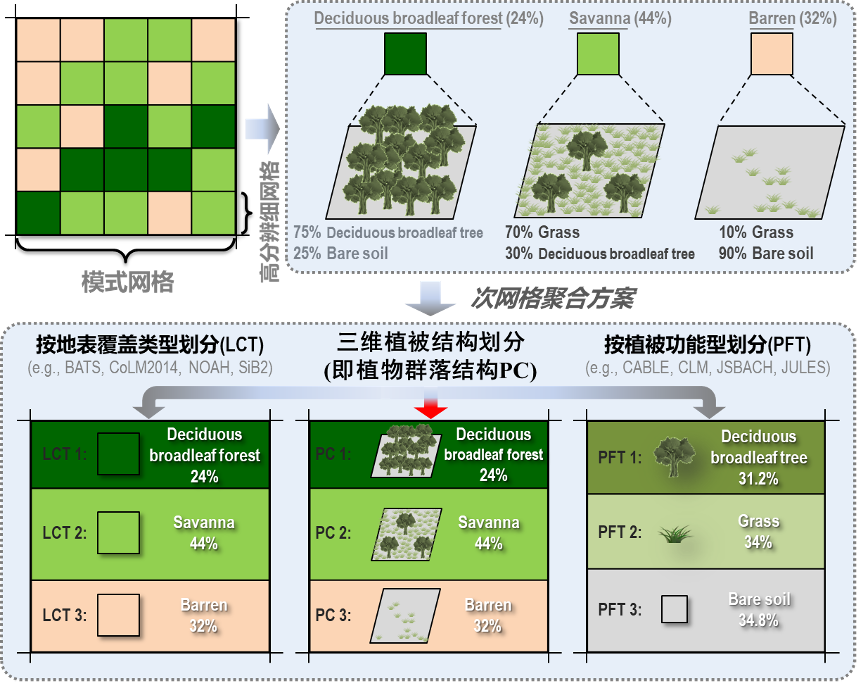
\includegraphics{Figures/地表输入数据/次网格聚合方案.png}
\caption{CoLM三种植被次网格聚合方案(LCT、PC和PFT)示意图}
\label{fig:次网格聚合方案}
\end{figure}
}


由于PFT和PC方案都需要对细网格地表覆盖数据进行PFT分解,而地表覆盖原数据并不包含此信息,
需要借助辅助数据进行计算,其数据来源如表 \ref{tab:网格划分辅助数据}所列。


% Please add the following required packages to your document preamble:
% \usepackage{booktabs}
% \usepackage[table,xcdraw]{xcolor}
% If you use beamer only pass "xcolor=table" option, i.e. \documentclass[xcolor=table]{beamer}
\begin{sidewaystable}[]
\centering
\caption{用于PFT和PC次网格划分辅助数据}
\label{tab:网格划分辅助数据}

\begin{tabular}[h]{p{3cm}p{6cm}p{2cm}p{2cm}p{5cm}}
\toprule
数据名称                                                            & 描述                                                                                              & 分辨率   & 坐标投影               & 参考文献                                            \\ \midrule
MODIS Land Cover Type & The Terra and Aqua combined MODIS Land Cover Type (LC\_Type1) data product, Version 6 (MCD12Q1) & 500 m & Sinusoidal        & (Friedl \& Sulla-Menashe, 2019)                \\\midrule
ESA LC-CCI land cover type                                      & ESA CCI land cover type products                                                                & 300 m & Latitude-Longitude & http://maps.elie.ucl.ac.be \\\midrule
MODIS VCF                                                       & MODIS Vegetation Continuous Fields product, Version 6 (MOD44B)                                           & 250 m & Sinusoidal         & \citet{DiMiceli2015}                        \\\midrule
AVHRR VCF                                                      & AVHRR Tree Cover (evergreen, deciduous and broadleaf, needleleaf) Continuous Fields                      & 1 km  & Latitude-Longitude & \citet{defries2000new}                         \\\midrule
Köppen-Geiger climate classification                                     & Present Köppen-Geiger climate classification maps at 1-km resolution                            & 1 km  & Latitude-Longitude & \citet{beck2018}                            \\\midrule
Reprocessed MODIS LAI                                           & Reprocessed MODIS leaf area index produces, Version 6                                           & 500 m & Sinusoidal         & \citet{yuan2011reprocessing}                              \\\midrule
WorldClim Version2                                             & Worldclim 2: New 1-km spatial resolution climate surfaces for global land areas                          & 1 km  & Latitude-Longitude & \citet{fick2017worldclim}                        \\\midrule
Canopy height                                                   & Global 1 km forest canopy height map                                                            & 1 km  & Latitude-Longitude & \citet{simard2011mapping}                          \\ \bottomrule
\end{tabular}
\end{sidewaystable}
如采用PFT/PC方案进行植被次网格模拟,其不同类型相关参数请参考附录 \ref{植被功能型PFT相关参数} 和附录 \ref{植物群落PC次网格PFT相关参数}。


\section{湖泊深度数据}\label{湖泊深度数据}
湖泊深度数据来自Lake-depth data set Version 2.0 \citep{kourzeneva2012global},数据为全球30$''$ (约1公里)分辨率,经纬度网格,单时次数据。


\section{城市数据}\label{城市数据}

\subsection{城市地表覆盖}\label{城市地表覆盖}
城市地表覆盖数据采用MODIS-IGBP地表覆盖数据(章节 \ref{IGBP地表覆盖数据})中的城市覆盖类型作为判别依据。
模式利用该数据集区分不同年份网格城市覆盖类型,获得城市在网格中的覆盖度,反应不同年份的城市覆盖变化。

\subsection{城市类型划分}\label{城市类型划分}
模式对城市覆盖地区不同城市类型进行细分。城市类型分类数据目前采取两种方案:
\begin{enumerate}
    \item 传统的3类城市——高建筑街区 (Tall Building Distinct, TBD)、高密度(High Density, HD) 和中密度 (Medium Density, MD);
    \item 10类Local Climate Zone (LCZ)分类,如图~\ref{fig:LCZ分类图示}  所示。
\end{enumerate}
{
\begin{figure}[]
\centering
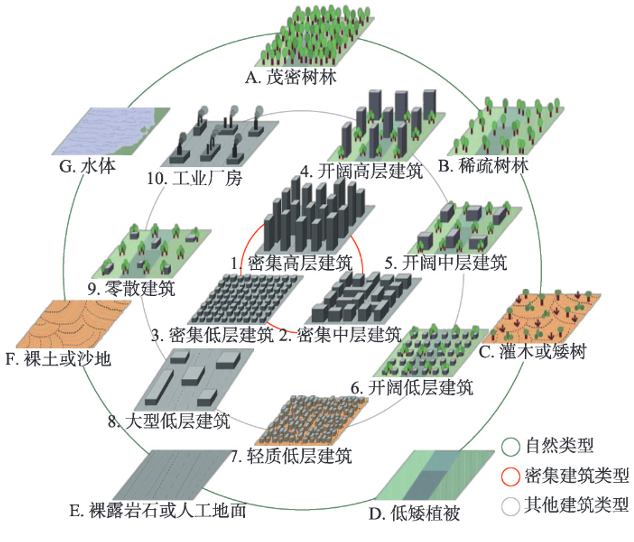
\includegraphics{Figures/地表输入数据/LCZ分类图示.png}
\caption{LCZ分类示意图}
\label{fig:LCZ分类图示}
\end{figure}
}


模式对于传统的城市类型分类与NCAR CLM--Urban Model \citep{oleson2020parameterization} 相同,
根据 \citet{jackson2013parameterization} 的城市分类数据对全球城市化程度进行分类。该数据集中,城市化有三个水平,
及TBD、HD和MD,每1km格点被划分为三个密度类别之一,通过该数据集对urban patch分为3类。其中,
TBD类城市指至少在1平方公里内,建筑高度全部大于或等于10层楼高且透水面比例较小(5$\sim$15\%);HD类城市建筑高度为3$\sim$10层,
透水面比例通常为5$\sim$25\%,这些地区通常为商业、住宅或工业区;MD类城市建筑高度通常为1$\sim$3层,且透水面比例较高,为20$\sim$60\%。
LCZ数据目前使用的 \citet{demuzere2022global} 全球LCZ分类数据,该数据空间分辨率为100米,
通过向轻量级随机森林模型输入大量标记训练区域和地球观测图像来生成,并对150个选定的功能城市地区采用自助交叉验证和专题基准测试评估了其质量。

\subsection{建筑形态及属性数据}\label{建筑形态及属性数据}
对于城市覆盖而言,建筑物的形态和物理性质(如反照率,导热率等)与其它地表覆盖类型完全不同,
这些物理性质取决于建筑物的材质及城市几何结构数据,比如: 不透水面比例分布(impervious fraction)、
建筑物屋顶面比例分布(roof fraction)、建筑物高度(building height)以及街区宽高比(H/W ratio)、反照率、发射率、导热率以及比热容等等。
目前使用 \citet{oleson2020parameterization} 基于 \citet{jackson2013parameterization} 的建筑数据开发的NCAR城市工具
(Toolbox for Human-Earth SystemIntegration \& Scaling (THESIS) toolset, http://www.cgd.ucar.edu/iam/projects/
thesis/thesis-urbanproperties-tool.html)为模式生成各类城市形态以及物理性质输入参数。
该工具根据一定规则将全球所有国家分为33类 (图 \ref{fig:地区分类}),并根据传统城市分类进一步划分,不同类的国家不同类型建筑具有不同的性质。
{
\begin{figure}[]
\centering
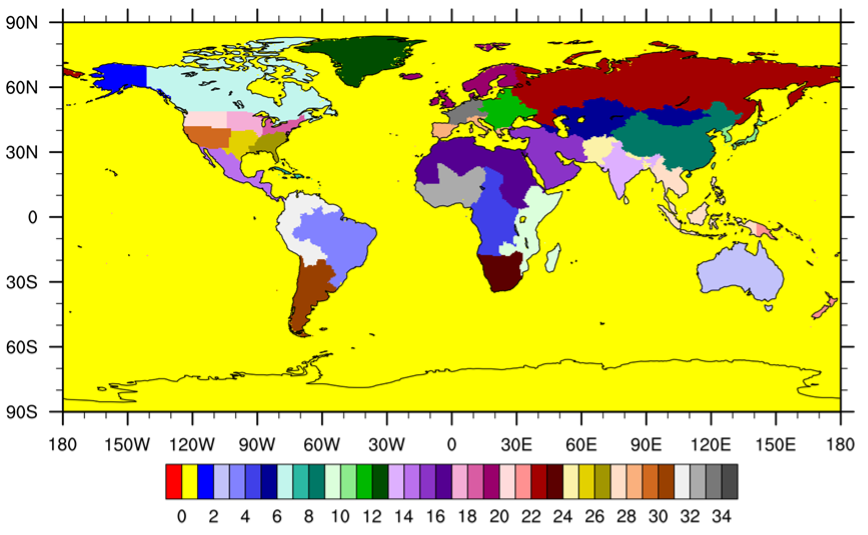
\includegraphics{Figures/地表输入数据/地区分类.png}
\caption{地区分类示意图}
\label{fig:地区分类}
\end{figure}
}
而LCZ分类本身包含了一些建筑材料信息,不同地区的同类LCZ虽然有差别但是可能不会太大,
因此LCZ形态参数目前采用典型值设定,该部分数据一部分来源于 \citet{stewart2014evaluation},另一部分参考了WRF中的参数设置。

\subsection{城市树覆盖数据}\label{城市树覆盖数据}
NCAR CLM城市数据集比较全面的描述了全球城市的形态特征和物理性质,但是其城市数据缺少关于植被(树)和水体的描述,
LCZ分类虽然有植被描述但通常是一个范围值。由于城市只占全球陆地的1\%左右,相比于自然地表,在大尺度上城市占比仍然比较小,
因此在补充城市内部的植被覆盖数据时,需要尽量选择高分辨率的数据。否则,如果分辨率过低,城市中的植被等信息很可能无法识别。
GFCC Tree Cover (https://lpdaac.usgs.gov/products/gfcc30tcv003/)提供了
2000年、2005年、2010年和2015年四个年代的全球树木覆盖度信息,分辨率为30m,可用于了解森林变化。
该数据的投影方式为UTM,与陆面模式使用的等经纬度网格不同,需对数据进行投影转换,由UTM投影转换为经纬度投影 (~0.00025$^\circ$)。
经过投影转换后,通过对全球数据每个区域的文件进行读取,并统计500m (\~0.0041667\textdegree)分辨率下30m高分辨网格植被总占比,
对四个年份求平均得到500m分辨率下城市格点的树覆盖数据作为城市模式的基础输入数据。

\subsection{城市内水体数据}\label{城市内水体数据}
基于与城市树覆盖同样的原因,水体数据也需要尽量选择高分辨率数据,30米全球地表覆盖数据GlobeLand30是中国研制的30米空间分辨率全球地表覆盖数据,
2014年发布GlobeLand30 2000和2010版。自然资源部于2017年启动对该数据的更新。目前,GlobeLand30 2020版已发布(http://www.globallandcover.com/)。
除极地地区外,GlobeLand30同样采用了UTM投影,因此需要进行投影转换,
其中数据覆盖如图~\ref{fig:GlobeLand30数据覆盖示意图} 所示(除2020年外,其他年份不包含极地地区数据)。
该数据集水体精度最高,达到了92.09\% \citep{陈军2017},且时空分辨率高,
因此投影转换后用同样的方法生成了水体覆盖度数据作为城市模式的原始数据。
{
\begin{figure}[]
\centering
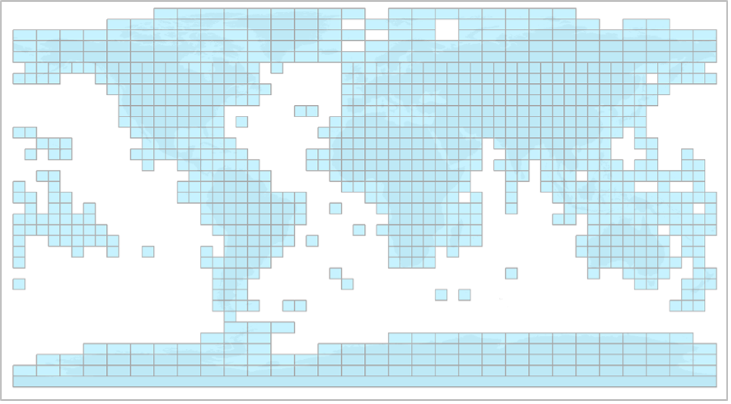
\includegraphics{Figures/地表输入数据/GlobeLand30数据覆盖示意图.png}
\caption{GlobeLand30数据覆盖示意图}
\label{fig:GlobeLand30数据覆盖示意图}
\end{figure}
}

\subsection{城市树高数据}\label{城市树高数据}
树高数据使用的 \citet{simard2011mapping} 全球树高数据,分辨率为1km。除该数据外, \citet{potapov2021mapping} 
利用GEDI卫星数据反演的30m树高数据也同样作为模式树高数据。但由于卫星运行轨道限制,
该数据目前只发布了51.6\textdegree N$\sim$51.6\textdegree S范围内的数据,北半球高纬度地区数据缺失,因此目前该数据集仅作为备用数据。

\subsection{城市LAI/SAI数据}\label{城市LAISAI数据}
由于城市中建筑物的遮掩,卫星反演数据中城市 LAI 存在一定问题,目前模式中城市 LAI 数据利用以下公式根据 0.5\textdegree 范围内的其它PFT (只考虑树,即1-9类PFT)的 LAI/SAI,通过插值并加权平均的办法为城市地区LAI/SAI赋值:
\begin{equation}
L A I_{u r}=\sum_{i=1}^{9} L A I_{P F T_{-} i} \cdot \frac{H T O P_{u r}}{H T O P_{P F T_{-} i}} \cdot P C T_{P F T_{-} i}
\end{equation}
其中$LAI_{PFT_{-}i}$为PFT的LAI(SAI),$HTOP_{ur}$和 $HTOP_{PFT_{-} i}$分别为城市树高和PFT树高,$PCT_{PFT_{-} i}$为PFT占比。城市树木SAI数据采用同样的方法进行计算。


%\end{地表输入数据}

\chapter{辐射过程及辐射通量计算}
%\addcontentsline{toc}{chapter}{辐射过程及辐射通量计算}
%\begin{辐射过程及辐射通量计算}
\section{土壤表面反照率}
反照率的计算3.1-3.6对应的代码文件为ALBEDO.F90。
土壤表面反照率采用陆面模式BATS方案 \citep{dickinson1986biosphere,dickinson1993biosphere},利用土壤颜色和土壤表层含水量计算得到,可表示为:
\begin{equation}
\alpha_{soi,vis,dir}=\operatorname{Min}\left(\alpha_{sat, vis}+\operatorname{Max}\left(0,0.11-0.40 \theta_{l}\right), \alpha_{dry, vis}\right)
\end{equation}
\begin{equation}
\alpha_{soi,nir,dir}=\operatorname{Min}\left(\alpha_{sat, nir}+\operatorname{Max}\left(0,0.11-0.40 \theta_{l}\right), \alpha_{dry, nir}\right)
\end{equation}
其中下标$soi$表示土壤,$vis$和$nir$分别表示可见光和近红外波段,$dir$表示直射光,$\alpha_{sat}$和$\alpha_{d r y}$是根据土壤颜色分类,通过查找表得到的饱和($sat$)和干($dry$)土壤的反照率数值,$\theta_{l}$为表层土壤体积含水量。目前土壤颜色数据采用CLM4.5全球20种颜色分类数据,包括可见光波段和近红外波段。漫射光与直射光相应波段一致。

\section{永久性冰川反照率}
对于永久性冰川覆盖地表,简单将可见光波段反照率设置为0.8,近红外波段设置为0.55,直射光与漫射光一致。


\section{内陆水体反照率}
对于液态水,可见光波段反照率为太阳天顶角余弦值$\mu$的函数,计算为$0.05/(\mu+0.15)$,近红外波段设置为常数0.1,
直射光与漫射光一致;当水体结冰,即地表温度小于273.16K时,可见光波段反照率设置为0.6,近红外波段设置为0.4,直射光与漫射光一致。

\section{雪盖表面反照率}
采用 \citet{dickinson1986biosphere} 方案,主要考虑太阳高度角和雪龄 (snow age) 两个主要参数,计算如下:
\begin{equation}
\alpha_{sno, vis, dir}=\alpha_{sno, vis, dif}+0.4 f(\mu)\left(1-\alpha_{sno, vis, dif}\right)
\end{equation}
\begin{equation}
\alpha_{sno,nir,dir}=\alpha_{sno, nir, dif}+0.4 f(\mu)\left(1-\alpha_{sno,nir,dif}\right)
\end{equation}   
\begin{equation}\label{alpha_sno_vis_dif}
\alpha_{sno,vis,dif}=0.85\left(1-0.2 F_{age}\right)
\end{equation}
\begin{equation}\label{alpha_sno_nir_dif}
\alpha_{sno,nir,dif}=0.65\left(1-0.5 F_{age}\right)
\end{equation}
其中下标$sno$表示雪盖,$f(\mu)$是一用来表征雪盖反照率与太阳高度角关系的参数化函数
\begin{equation}\label{fmu}
f(\mu)=\operatorname{Max}\left[0,\left(\frac{1.5}{1+4 \mu}-0.5\right)\right]
\end{equation}
公式(\ref{alpha_sno_vis_dif}),(\ref{alpha_sno_nir_dif})中0.85和0.65分别表示可见光和近红外波段新雪反照率,
$F_{age}$表示雪龄,使得雪的反照率随着雪盖中雪晶颗粒的增长和灰尘等杂质的积累而减少,其计算为
\begin{equation}
F_{a g e}=\frac{\tau_{sno}}{1+\tau_{sno}}
\end{equation}
$\tau_{sno}$是一预报变量,它随时间的增量函数为
\begin{equation}
\Delta \tau_{sno}=1 \times 10^{-6}\left(r_{1}+r_{2}+r_{3}\right) \Delta t
\end{equation}
其中$\Delta t$是积分时间步长($s$),
\begin{equation}
r_{1}=\exp \left[5000\left(\frac{1}{273.16}-\frac{1}{T_{g}}\right)\right]
\end{equation}
\begin{equation}
r_{2}=r_{1}^{10} \leq 1
\end{equation}
\begin{equation}
r_{3}=0.3
\end{equation}
上式中,$r_1$表示雪盖中水汽的扩散导致的雪晶颗粒增长对反照率的影响,$r_2$表示融雪对反照率的影响,$r_3$表示灰尘或杂质的影响。
为了考虑新降雪的影响,在$\tau_{sno}$的计算中还包含计算时间步长内的降雪量,表示为
\begin{equation}
\tau_{sno}^{N+1}=\left(\tau_{sno}^{N}+\Delta \tau_{sno}\right)\left(1-100 \Delta p_{s}\right)
\end{equation}
其中$\Delta p_{s}$为在$t^(N+1)$-$t^N$时间内的降雪量(m),$N$为积分的时间步数。


对于部分雪覆盖的地表,其反照率为雪覆盖度($f_{sno}$,参见章节 \ref{无植被覆盖地表湍流通量的计算方案})的加权函数,表示为:
\begin{equation}
\alpha_{g}=\left(1-f_{sno}\right) * \alpha_{g}+f_{sno} \alpha_{sno}
\end{equation}
其中$\alpha_{g}$表示土壤、冰川或水体地表覆盖时的反照率。对可见光和近红外波段均按上式计算。

\section{海洋和海冰反照率}\label{海洋和海冰反照率}
对应代码为ALBEDO.F90。注:需进一步补充
对于海冰,根据冰和雪的反照率综合计算。计算公式如下(待补充):

对于无冰海洋,采用太阳高度角计算直射入射反照率,漫射反射率则设为常数。计算中,假设反照率与波段和海表面风速等其他物理量无关。可见光和近红外波段的漫射反射率均设为0.06;而两个波段的直射反照率均通过以下公式计算:
\begin{equation}
\alpha_{s}= \frac{0.026}{\mu^{1.7}+0.065}+0.15*(\mu-0.1)*(\mu-0.5)*(\mu-1) 
\end{equation}

\section{植被反照率-二流近似模型}\label{植被反照率二流近似模型}
{
\begin{figure}[]
\centering
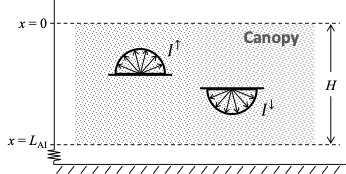
\includegraphics{Figures/辐射过程及辐射通量计算/二流近似模型示意图.png}
\caption{植被辐射传输二流近似模型示意图}
\label{fig:二流近似模型示意图}
\end{figure}
}
植被反照率采用二流近似方法(two-stream approximation, \citet{dickinson1983land,sellers1985canopy} )进行求解。在此基础上,利用双大叶模型(two-big-leaf model) \citep{dai2004two} 对阴阳叶分别计算辐射吸收量。二流近似方法是把植被冠层内的辐射场看成是上下两个辐射流组成(图 \ref{fig:二流近似模型示意图}),这样可以把描述辐射传输的微分方程简化为两个联立的常微分方程组:
\begin{equation}\label{di_dx1}
-\bar{\mu} \frac{d I^{\uparrow}}{d x}+\{1-(1-\beta) \omega\} I^{\uparrow}-\omega \beta I^{\downarrow}=\omega \bar{\mu} K \beta_{0} \exp (-K x)
\end{equation}
\begin{equation}\label{di_dx2}
\bar{\mu} \frac{d I^{\downarrow}}{d x}+\{1-(1-\beta) \omega\} I^{\downarrow}-\omega \beta I^{\uparrow}=\omega \bar{\mu} K\left(1-\beta_{0}\right) \exp (-K x)
\end{equation}
其中$I^{\uparrow}$, $I^{\downarrow}$表示向上和向下的漫射通量,为相对于总入射辐射通量(含直射和漫射)的归一化值。$\mu$为太阳天顶角余弦,$\bar{\mu}$为漫射辐射在单位叶面积上的光学厚度倒数平均值。$\beta$、$\beta_{0}$为漫射辐射和直射辐射向上散射(upscatter)系数,$\omega$为叶片单次散射反照率,等于叶片反射率$\rho_{l}$和透射率$\tau_{l}$之和。$K$为直射光在单位叶面积上的光学厚度,计算为$G(\mu) / \mu$,其中$G(\mu)$为叶子在入射辐射方向上的投影面积。$x$表示植被从冠层顶部($x=0$)往下($x=LAI$)累积的叶面积指数。

$G(\mu) / \mu$函数采用 \citet{goudriaan1977crop} 方案,它使用一个参数$\chi_{L}  $\citep{ross1975radiative} 去描述植被的叶倾角分布:
\begin{equation}\label{Gmu}
G(\mu)=\phi_{1}+\phi_{2} \mu
\end{equation}
其中$\phi_{1}=0.5-0.633 \chi_{L}-0.33 \chi_{L}^{2}, \phi_{2}=0.877\left(1-2 \phi_{1}\right)$,
\begin{equation}
\chi_{L}=\pm \int_{0}^{\frac{\pi}{2}}\left|\sin \theta_{L}-f_{S}\left(\theta_{L}\right)\right| d \theta_{L}
\end{equation}
上式中$\sin \theta_{L}$为球形叶倾角分布函数,$f_{S}\left(\theta_{L}\right)$为植被的叶倾角分布函数。
因此,对于球形分布来说,$\chi_{L}=0$。 一般来讲,$-0.4≤\chi_{L}≤0.6$,分别对应竖直型和平面型叶倾角分布。
模型中实际应用时采用通过查找表得到的不同植被类型$\chi_{L}$设定值。根据$G(\mu)$的表达式,$\bar{\mu}$可以计算为
\begin{equation}
\bar{\mu}=\int_{0}^{1} \frac{\mu^{\prime}}{G\left(\mu^{\prime}\right)}
 d \mu^{\prime}=\frac{1}{\phi_{2}}\left\{1-\frac{\phi_{1}}{\phi_{2}}
 \ln \left(\frac{\phi_{1}+\phi_{2}}{\phi_{1}}\right)\right\}
\end{equation}
上面计算表达式是假设$\phi_{1} \neq 0$以及$\phi_{2} \neq 0$,但实际上两者均可为0 \citep{dai2004two}。当$\phi_{1}$、$\phi_{2}$为0时,计算为
\begin{equation}
\bar{\mu}=1 / 0.877, \text { 当 } \phi_{1}=0
\end{equation}
\begin{equation}
\bar{\mu}=1 /\left(2 \phi_{1}\right), \text { 当 } \phi_{2}=0
\end{equation}
假设叶片上的散射辐射各项同性(理想朗伯体),漫射辐射和直射辐射向上散射系数$\beta$、$\beta_0$可近似计算为
\begin{equation}
\omega \beta=\frac{1}{2}\left[\rho_{l}+\tau_{l}+\left(\rho_{l}-\tau_{l}\right)\left(\frac{1+\chi_{L}}{2}\right)^{2}\right]
\end{equation}
\begin{equation}\label{beta0}
\beta_{0}=\frac{1+\bar{\mu} K}{\omega \bar{\mu} K} a_{s}(\mu)
\end{equation}
其中$\rho_l$和$\tau_l$表示叶片的反射率和透射率,
并依赖于波段,$\omega=\rho_l+\tau_l$。$a_s$为当植被为无穷厚时($LAI\rightarrow\infty$),
整个植被的单次散射反照率,计算为
\begin{equation}
\begin{aligned} a_{s} &=\frac{\omega}{2} \int_{0}^{1} \frac{\mu G\left(\mu^{\prime}\right)}{\mu G\left(\mu^{\prime}\right)+\mu^{\prime} 
G(\mu)} d \mu^{\prime} \\ &=\frac{\omega}{2} \frac{G(\mu)}{G(\mu)+\mu \phi_{2}}\left[1-\frac{\mu \phi_{1}}{G(\mu)+\mu \phi_{2}} 
\ln \left(\frac{G(\mu)+\mu \phi_{1}+\mu \phi_{2}}{\mu \phi_{1}}\right)\right] \end{aligned}
\end{equation}
对于方程(\ref{di_dx1})和(\ref{di_dx1}),直射入射情况下(即假定通过冠层顶部向下的漫射辐射通量等于0),其边界条件为
\begin{equation}
I^{\downarrow}=0 \text {, 当 } x=0 \text { 时 }
\end{equation}
\begin{equation}
I^{\uparrow}=\alpha_{g, dif} I^{\downarrow}+\alpha_{g, dir} \exp \left(-K LAI \right) \text {, 当 } x=LAI \text { 时 }
\end{equation}
方程的解为
\begin{equation}
I^{\uparrow}=h_{1} e^{-K x / \sigma}+h_{2} e^{-h x}+h_{3} e^{h x}
\end{equation}
\begin{equation}
I^{\downarrow}=h_{4} e^{-K x / \sigma}+h_{5} e^{-h x}+h_{6} e^{h x}
\end{equation}
因此可以得到在冠层顶部的漫射辐射通量(即反照率)为
\begin{equation}
\alpha_{veg, dir}=I^{\uparrow}(0)=\frac{h_{1}}{\sigma}+h_{2}+h_{3}
\end{equation}
到达地面的辐射通量为
\begin{equation}
\tau_{veg, dir}=I^{\downarrow}\left(L_{A I}\right)=\frac{h_{4}}{\sigma} e^{-K} L_{A I}+h_{5} e^{-h L_{A I}}+h_{6} e^{h L_{A I}}
\end{equation}
漫射入射辐射时,边界条件为
\begin{equation}
I^{\downarrow}=1 \text {, 当 } x=0 \text { 时 }
\end{equation}
\begin{equation}
I^{\uparrow}=\alpha_{g, dif} I^{\downarrow} \text {, 当 } x=L_{A I} \text { 时 }
\end{equation}
方程的解为
\begin{equation}
I^{\uparrow}=h_{7} e^{-h x}+h_{8} e^{h x}
\end{equation}
\begin{equation}
I^{\downarrow}=h_{9} e^{-h x}+h_{10} e^{h x}
\end{equation}
因此可以得到在冠层顶部的漫射辐射通量(即反照率)为
\begin{equation}
\alpha_{veg, dif}=I^{\uparrow}(0)=h_{7}+h_{8}
\end{equation}
到达地面的漫射辐射通量为
\begin{equation}
\tau_{veg, dif}=I^{\downarrow}\left(L_{A I}\right)=h_{9} e^{-h L_{A I}}+h_{10} e^{h L_{A I}}
\end{equation}
以上$\sigma,h_1,h_2,\ldots,h_{10}$计算为[参考\citet{sellers1985canopy}附录,注$h_4$在原文中有误,下面为修改后计算式]
\begin{equation}
b=1-\omega+\omega \beta
\end{equation}
\begin{equation}
c=\omega \beta
\end{equation}
\begin{equation}
d=\omega \bar{\mu} K \beta_{0}
\end{equation}
\begin{equation}
f=\omega \bar{\mu} K\left(1-\beta_{0}\right)
\end{equation}
\begin{equation}
h=\frac{\sqrt{b^{2}-c^{2}}}{\bar{\mu}}
\end{equation}
\begin{equation}
\sigma=(\bar{\mu} K)^{2}+c^{2}-b^{2}
\end{equation}
\begin{equation}
u_{1}=b-c / \alpha_{g, dif}
\end{equation}
\begin{equation}
u_{2}=b-c \alpha_{g, dif}
\end{equation}
\begin{equation}
u_{3}=f+c \alpha_{g, dif}
\end{equation}
\begin{equation}
s_{1}=\exp \left\{-\min \left[h L_{A I}, 50\right]\right\}
\end{equation}
\begin{equation}
s_{2}=\exp \left\{-\min \left[K L_{A I}, 50\right]\right\}
\end{equation}
\begin{equation}
p_{1}=b+\bar{\mu} h
\end{equation}
\begin{equation}
p_{2}=b-\bar{\mu} h
\end{equation}
\begin{equation}
p_{3}=b+\bar{\mu} K
\end{equation}
\begin{equation}
p_{4}=b-\bar{\mu} K
\end{equation}
\begin{equation}
d_{1}=\frac{p_{1}\left(u_{1}-\bar{\mu} h\right)}{s_{1}}-p_{2}\left(u_{1}+\bar{\mu} h\right) s_{1}
\end{equation}
\begin{equation}
d_{2}=\frac{u_{2}+\bar{\mu} h}{s_{1}}-\left(u_{2}-\bar{\mu} h\right) s_{1}
\end{equation}
\begin{equation}
h_{1}=-d p_{4}-c f
\end{equation}
\begin{equation}
h_{2}=\frac{1}{d_{1}}\left[\left(d-\frac{h_{1}}{\sigma} p_{3}\right)\left(u_{1}-\bar{\mu} h\right) 
\frac{1}{s_{1}}-p_{2}\left(d-c-\frac{h_{1}}{\sigma}\left(u_{1}+\bar{\mu} K\right)\right) s_{2}\right]
\end{equation}
\begin{equation}
h_{3}=-\frac{1}{d_{1}}\left[\left(d-\frac{h_{1}}{\sigma}\right)\left(u_{1}+\bar{\mu} h\right) 
s_{1}-p_{1}\left(d-c-\frac{h_{1}}{\sigma}\left(u_{1}+\bar{\mu} K\right)\right) s_{2}\right]
\end{equation}
\begin{equation}
h_{4}=-f p_{3}-c d
\end{equation}
\begin{equation}
h_{5}=-\frac{1}{d_{2}}\left[\frac{h_{4}}{\sigma}\left(u_{2}+\bar{\mu} h\right) 
\frac{1}{s_{1}}+\left(u_{3}-\frac{h_{4}}{\sigma}\left(u_{2}-\bar{\mu} K\right)\right) s_{2}\right]
\end{equation}
\begin{equation}
h_{6}=\frac{1}{d_{2}}\left[\frac{h_{4}}{\sigma}\left(u_{2}-\bar{\mu} h\right) 
s_{1}+\left(u_{3}-\frac{h_{4}}{\sigma}\left(u_{2}-\bar{\mu} K\right)\right) s_{2}\right]
\end{equation}
\begin{equation}
h_{7}=\frac{c\left(u_{1}-\bar{\mu} h\right)}{d_{1} s_{1}}
\end{equation}
\begin{equation}
h_{8}=\frac{-c\left(u_{1}+\bar{\mu} h\right) s_{1}}{d_{1}}
\end{equation}
\begin{equation}
h_{9}=\frac{u_{2}+\bar{\mu} h}{d_{2} s_{1}}
\end{equation}
\begin{equation}
h_{10}=\frac{-s_{1}\left(u_{2}-\bar{\mu} h\right)}{d_{2}}
\end{equation}
以上解严格上是在$\sigma \neq 0$时成立,当$\sigma = 0$时,\citet{dai2004two} 给出了直射入射时的解为
\begin{equation}
I^{\uparrow}=h_{2}^{\prime} e^{-K x}+h_{3}^{\prime} e^{K x}-\frac{h 1}{\bar{\mu}^{2}}\left(x+\frac{1}{2 K}\right) e^{-K x}
\end{equation}
\begin{equation}
I^{\downarrow}=h_{5}^{\prime} e^{-K x}+h_{6}^{\prime} e^{K x}+\frac{1}{c}\left\{-\frac{1}{2 K}
 \frac{h_{1}}{\overline{\mu^{2}}}\left(p_{3} x+p_{4} \frac{1}{2 K}\right)-d\right\} e^{-K x}
\end{equation}
其中
\begin{equation}
h_{2}^{\prime}=\left(m_{3} p_{2}-m_{2} n_{3}\right) /\left(m_{1} p_{2}-m_{2} p_{1}\right)
\end{equation}
\begin{equation}
h_{3}^{\prime}=\left(m_{3} p_{1}-m_{1} n_{3}\right) /\left(m_{2} p_{1}-m_{1} p_{2}\right)
\end{equation}
\begin{equation}
h_{5}^{\prime}=h_{2}^{\prime} p_{1} / c
\end{equation}
\begin{equation}
h_{6}^{\prime}=h_{3}^{\prime} p_{2} / c
\end{equation}
\begin{equation}
m_{1}=\left(1-\alpha_{g, dif} p_{1} / c\right) s_{1}
\end{equation}
\begin{equation}
m_{2}=\left(1-\alpha_{g, dif } p_{2} / c\right) s_{1}
\end{equation}
\begin{equation}
\begin{aligned} m_{3} &=\frac{h_{1}}{\bar{\mu}^{2}}\left(L_{A I}+\frac{1}{2 K}\right) s_{2} \\ &+\alpha_{g, \text { dif }}
 \frac{1}{c}\left\{-\frac{1}{2 K} \frac{h_{1}}{\bar{\mu}^{2}}\left(p_{3} L_{A I}+p_{4} \frac{1}{2 K}\right)-d\right\} s_{2} \\ 
 &+\alpha_{g, \text { dir }} s_{2} \end{aligned}
\end{equation}
\begin{equation}
n_{3}=\frac{1}{4 K^{2}} \frac{h_{1}}{\bar{\mu}^{2}} p_{4}+d
\end{equation}
植被吸收的辐射通量为
\begin{equation}
I_{veg, dir}=1-\alpha_{veg, dir}-\left(1-\alpha_{g, dif}\right) \tau_{veg, dir}-\left(1-\alpha_{g, \text { dir }}\right) s_{2}
\end{equation}
\begin{equation}
I_{veg, dif}=1-\alpha_{veg, dif}-\left(1-\alpha_{g,dif}\right) \tau_{veg, dif}
\end{equation}
\citet{dai2004two} 将植被分为阴叶和阳叶来计算其各自辐射通量吸收,对于直射入射光,阳叶、阴叶吸收辐射通量分别如下
\begin{equation}
I_{\text {sun,dir }}=(1-\omega)\left[1-s_{2}+\frac{1}{\bar{\mu}}\left(a_{1}+a_{2}\right)\right]
\end{equation}
\begin{equation}
I_{\text {sha,dir }}=I_{\text {veg,dir }}-I_{\text {sun,dir }}
\end{equation}
其中
\begin{equation}
a_{1}=\frac{h_{1}}{\sigma}\left[\frac{1-s_{2}^{2}}{2 K}\right]+h_{2}\left[\frac{1-s_{2} s_{1}}{K+h}\right]+h_{3}\left[\frac{1-s_{2} / s_{1}}{K-h}\right]
\end{equation}
\begin{equation}
a_{2}=\frac{h_{4}}{\sigma}\left[\frac{1-s_{2}^{2}}{2 K}\right]+h_{5}\left[\frac{1-s_{2} s_{1}}{K+h}\right]+h_{6}\left[\frac{1-s_{2} / s_{1}}{K-h}\right]
\end{equation}
对于漫射光源,阳叶、阴叶吸收辐射通量分别如下
\begin{equation}
I_{sun,dif}=\left[\frac{1-\omega}{\bar{\mu}}\right]\left(a_{1}+a_{2}\right)
\end{equation}
\begin{equation}
I_{\text {sha,dir }}=I_{veg, dir}-I_{\text {sun,dir }}
\end{equation}
其中
\begin{equation}
a_{1}=h_{7}\left[\frac{1-s_{2} s_{1}}{K+h}\right]+h_{8}\left[\frac{1-s_{2} / s_{1}}{K-h}\right]
\end{equation}
\begin{equation}
a_{2}=h_{9}\left[\frac{1-s_{2} s_{1}}{K+h}\right]+h_{10}\left[\frac{1-s_{2} / s_{1}}{K-h}\right]
\end{equation}
注意,以上公式对于可见光波段和近红外波段均成立,为了简化公式表达形式,波段标识信息均已省略。


当植被部分面积比例($wt$,参见章节 \ref{无植被覆盖地表湍流通量的计算方案})被雪掩埋时,则植被的反照率修改为
\begin{equation}
\alpha_{veg}=(1-w t) \alpha_{veg}+w t \cdot \alpha_{sno}
\end{equation}
不同波段及直射/漫射情景均按以上加权方式计算。考虑植被覆盖度($f_{veg}$)时的地表反照率为

\begin{equation}\label{alpha1}
\alpha=\left(1-f_{veg}\right) \alpha_{g}+f_veg \alpha_{veg}
\end{equation}
同样,以上公式适用于可见光和近红外波段,以及直射和漫射入射辐射情况。


\section{改进的二流近似植被辐射传输模型}
根据 \citet{yuan2017reexamination} 对目前二流近似植被辐射传输参数化方案的对比分析,对章节 \ref{植被反照率二流近似模型} 方案进行改进,主要包括两个方面:
\begin{enumerate}
    \item 入射漫射辐射计算;
    \item 向上散射系数$\beta_0$ [原公式(\ref{beta0})] 计算。
\end{enumerate}

对于球形叶倾角分布($\chi_L=0$)情景,植被在漫射光入射时的透射率表示为
\begin{equation}
T_{d}^{*}=2 \int_{0}^{1} \exp \left(-\frac{G(\mu) LAI}{\mu}\right) \mu d \mu, G(\mu)=0.5
\end{equation}
由于以上公式没有解析解,通过不完全伽玛函数展开式,以上公式可近似表达为
\begin{equation}
T_{d}^{*} \approx \frac{\exp (-0.5 a LAI)}{1+0.5 b LAI}
\end{equation}
通过与数值积分结果拟合得到$a=0.87$, $b=0.92$ (对于$0<LAI<8$,$RSME=0.002$)。因此,等效的漫射辐射入射角度(类似于直射辐射入射角度)可表示为:
\begin{equation}
\exp \left(-\frac{0.5 LAI}{\mu^{*}}\right)=\frac{\exp (-0.5 a LAI)}{1+0.5 b LAI}
\end{equation}
即
\begin{equation}
\mu^{*}=-0.5 LAI \cdot \ln ^{-1} \frac{\exp (-0.5 a LAI)}{1+0.5 b LAI}
\end{equation}

对于非球形叶倾角分布情况,$\mu^\ast$可修订为:
\begin{equation}
\mu^{*}=\cos \left(\operatorname{acos}\left(\mu^{*}\right)+5 \chi_{L}\right)
\end{equation}
上式右边$\operatorname{acos}\left(\mu^{*}\right)$为球形叶倾角分布时的结果(单位表示为角度$^{\circ}$)。


对于向上散射系数$\beta_0$,CoLM2014是沿用Dickinson and Sellers方案\citep{dickinson1983land,sellers1985canopy},
其中有一个较不合理的假设是认为叶子的体散射为均一散射,这对入射直射辐射引入一定的误差。在新版CoLM中,采用SAIL模型计算方案
\begin{equation}
\omega \beta_{0}=\frac{1}{2}\left[\omega+\frac{\mu}{G(\mu)} \delta \int_{0}^{\pi / 2} 
f\left(\theta_{l}\right) \cos ^{2}\left(\theta_{l}\right) \sin \left(\theta_{l}\right) d \theta_{l}\right]
\end{equation}
其中$f\left(\theta_l\right)$为叶倾角分布函数。因为在CLM中叶倾角分布是用$\chi_l$参数来描述,
上式中的积分表达式无法算出,这里沿用CLM的计算方法,使用等效(或说平均)叶倾角$\bar{\theta_l}$来计算,即
\begin{equation}
\omega \beta_{0}=\frac{1}{2}\left[\omega+\frac{\mu}{G(\mu)} \delta \cos ^{2}\left(\overline{\theta_{l}}\right)\right]
\end{equation}
上式中$\delta=\rho_l-\tau_l$。平均叶倾角计算为
\begin{equation}
\cos \left(\overline{\theta_{l}}\right)=\frac{1+\chi_{L}}{2}
\end{equation}
新改进的二流近似模型在实际应用中先假设土壤反照率为0 (black background),从而计算在入射直射(漫射)辐射时的直射透射率$T_d$ ($T_d^\ast$),
漫射透射率$T_i$ ($T_i^\ast$),反照率$\alpha$ ($\alpha^\ast$) 以及植被吸收率$A$ ($A^\ast$)。
根据以上结果,考虑土壤反照率不为0时的植被与土壤之间的多次散射/吸收过程,此时从土壤反射的辐射考虑为漫射辐射,
采用以上描述的改进的二流近似方案进行处理。在植被-土壤多次反射达到平衡时,总的植被透射率计算为
\begin{equation}
[T]=\frac{T}{1-q}
\end{equation}
上式右边$T$为土壤反射率为0时总的透射率(直射入射情景 $T=T_d+T_i$,漫射入射情景 $T=T_d^\ast+T_i^\ast$)、$q=r_g\alpha^\ast$。
对于直射入射情景,总的植被吸收为$\left[A\right]=A+r_g\left[T\right]A^\ast$,
总的土壤吸收为$\left[G\right]=\left(1-r_g\right)\left[T\right]$,
总的反照率$\left[\alpha\right]=1-\left[A\right]-\left[G\right]$。漫射入射时计算方式类似。
新方案同样会改变阴阳面辐射吸收比例,其中直射入射辐射阳面吸收为
\begin{equation}
I_{sun,dir}=(1-\omega)\left[1-s_{2}+\frac{1}{\bar{\mu}}\left(a_{1}+a_{2}\right)\right]
\end{equation}
\begin{equation}
I_{sha,dir}=I_{veg,dir}-I_{sun,dir}
\end{equation}
对于漫射入射辐射
\begin{equation}
I_{sun,dif}=(1-\omega)\left[K\left(1-s_{2} s_{2}^{\prime}\right)+\frac{1}{\bar{\mu}}\left(a_{1}+a_{2}\right)\right]
\end{equation}
\begin{equation}
I_{sha,dif}=I_{veg,dif}-I_{sun,dif}
\end{equation}
其中
\begin{equation}
a_{1}=\frac{h_{1}}{\sigma}\left[\frac{1-s_{2} s_{2}^{\prime}}{K+K^{\prime}}\right]+h_{2}\left[\frac{1-s_{2}^{\prime} 
s_{1}}{K^{\prime}+h}\right]+h_{3}\left[\frac{1-s_{2}^{\prime} / s_{1}}{K^{\prime}-h}\right]
\end{equation}
\begin{equation}
a_{2}=\frac{h_{4}}{\sigma}\left[\frac{1-s_{2} s_{2}^{\prime}}{K+K^{\prime}}\right]+h_{5}\left[\frac{1-s_{2}^{\prime} s_{1}}
{K^{\prime}+h}\right]+h_{6}\left[\frac{1-s_{2} / s_{1}}{K^{\prime}-h}\right]
\end{equation}
当为入射直射辐射时,$s_2^\prime=s_2$、$K^\prime=K$;当为入射漫射辐射时$s_2^\prime$、$K^\prime$为漫射辐射对应的等效直射角度时的$s$和$K$值。


对于土壤反射部分的漫射光源在阳叶面的吸收不同于天空漫射光源在阳叶面的吸收,计算为:
\begin{equation}
I_{s u n, dif}=s_{2}^{\prime}(1-\omega)\left[K\left(1-\frac{s_{2}}{s_{2}^{\prime}}\right)
\left(K-K^{\prime}\right)+\frac{1}{\bar{\mu}}\left(a_{1}+a_{2}\right)\right]
\end{equation}
其中
\begin{equation}
a_{1}=\frac{h_{1}}{\sigma}\left[\frac{1-s_{2} / s_{2}^{\prime}}{K-K^{\prime}}\right]+h_{2}\left[\frac{1-s_{1} /
 s_{2}^{\prime}}{h-K^{\prime}}\right]+h_{3}\left[\frac{1 / s_{1} / s_{2}^{\prime}-1}{h+K^{\prime}}\right]
\end{equation}
\begin{equation}
a_{2}=\frac{h_{4}}{\sigma}\left[\frac{1-s_{2} / s_{2}^{\prime}}{K-K^{\prime}}\right]+h_{5}\left[\frac{1-s_{1} / 
s_{2}^{\prime}}{h-K^{\prime}}\right]+h_{6}\left[\frac{1 / s_{1} / s_{2}^{\prime}-1}{h+K^{\prime}}\right]
\end{equation}
另外,相比于CoLM2014,植被的光学属性不仅考虑叶片的影响,同时也加入了茎的影响,“叶片”等效的光学属性为叶片
和茎光学属性按照其各自面积($LAI$, $SAI$)的加权平均(在上述文档中为了简化,保留原来$\rho_l$和$\tau_l$符号,
但其物理含义已是叶片和茎光学属性的加权值,即等效叶片光学属性)。



\section{短波吸收辐射通量}\label{短波吸收辐射通量}
此部分对应代码为netsolar.F90。
在计算得到地表反照率后,地表总的太阳短波辐射通量(包括地面和植被)吸收为
\begin{equation}
F_{v g}=F_{vis,dir}\left(1-\alpha_{vis,dir}\right)+F_{vis,dif}\left(1-\alpha_{vis,dif}\right)+
F_{nir,dir}\left(1-\alpha_{nir,dir}\right)+F_{nir,dif}\left(1-\alpha_{nir,dif}\right)
\end{equation}
其中等式右边F表示太阳短波在不同波段($vis$、$nir$)和直射/漫射时的辐射通量。阳叶、阴叶辐射通量吸收分别为
\begin{equation}
F_{s u n}=F_{vi s, dir} I_{s u n, vi s, dir}+F_{vis, dif} \alpha_{s u n, vis, dif}+F_{ni r, dir} \alpha_{s u n, ni r, dir}+F_{nir, dif} \alpha_{s u n, nir, dif}
\end{equation}
\begin{equation}
F_{s h a}=F_{vi s, dir} I_{\text {sun,vis,dir }}+F_{vis, dif} \alpha_{\text {sun,vis,dif }}+F_{ni r, dir} \alpha_{\text {sun,nir,dir }}+F_{nir, dif} \alpha_{\text {sun,nir,dif }}
\end{equation}
考虑植被覆盖度及雪的掩埋,阳叶、阴叶的吸收修改为$f_{sig}F_{sun}$和$f_{sig}F_{sha}$,其中$f_{sig}$为网格有效植被覆盖率(参见章节 \ref{无植被覆盖地表湍流通量的计算方案})。地面的吸收辐射通量值
\begin{equation}
F_{g}=F_{v g}-F_{s u n}-F_{s h a}
\end{equation}
单位面积阳叶、阴叶有效光合辐射吸收通量为
\begin{equation}
P A R_{\text {sun }}=F_{vi s, dir} I_{\text {sun,vis,dir }}+F_{vis, dif} I_{s u n, vis, dif}
\end{equation}

\begin{equation}
P A R_{s h a}=F_{vi s, dir} I_{\text {sha,vis,dir }}+F_{vis, dif} I_{\text {sha,vis,dif }}
\end{equation}


\section{长波净辐射通量}\label{长波净辐射通量}
此部分对应代码为THERMAL.F90。
地表发射的长波辐射是基于斯蒂芬-玻尔兹曼定律来计算。
当为土壤时,地面发射率$\varepsilon_g$设置为0.96;对于冰川时,设置为0.97。
裸土覆盖下,地面的长波净辐射通量计算为
\begin{equation}
L W_{g}=\varepsilon_{g} F_{a}
\end{equation}
其中$F_a$表示大气向下长波辐射通量。
对于植被覆盖地面,植被长波发射率(吸收率)计算为
\begin{equation}
\varepsilon_{v}=1-\exp \left(-\frac{LAI+SAI}{\bar{\mu}}\right)
\end{equation}
其中$SAI$表示植被茎面积指数。植被的长波净辐射通量计算为
\begin{equation}
L W_{v}=\varepsilon_{v}\left(F_{a}-2 \sigma T_{l}^{4}+\varepsilon_{g} \sigma T_{g}^{4}\right)
\end{equation}
其中$T_l$表示叶片温度,$T_g$表示土壤表层温度,$\sigma$表示斯蒂芬-玻尔兹曼常数。
注意,以上的计算并未考虑植被向下长波辐射到达地面后的反射部分,即假设全部被地面吸收。在新版本中,考虑一次土壤反射,然后被植被吸收,其计算表达式为
\begin{equation}
L W_{v}=\varepsilon_{v}\left(F_{a}-2 \sigma T_{l}^{4}+\varepsilon_{g} \sigma T_{g}^{4}\right)+\left(1-\varepsilon_{g}\right)\left(1-\varepsilon_{v}\right) \varepsilon_{v} F_{a}+\left(1-\varepsilon_{g}\right) \varepsilon_{v}^{2} \sigma T_{l}^{4}
\end{equation}
如叶温区分阴阳叶时,长波净辐射根据其各自叶片温度分开计算。格点植被有效覆盖面积不为100\%时,其长波净辐射通量按地面和植被面积比例进行加权平均。

\section{三维植被辐射传输模型}\label{三维植被辐射传输模型}
此部分对应的代码为ThreeDCanopy.F90。
三维植被辐射传输模型\citep{yuan20143d}是在单棵树冠模型\citep{dickinson2008determination,dickinson2008three}的基础上建立起来的(图\ref{fig:三维植被辐射传输模型的基本框架})。
利用单棵树冠模型来建立单层植被模型,考虑了植被阴影的影响、植被树冠之间的散射吸收及低入射角度(太阳高度角)对反照率的影响。通过考虑层与层之间阴影相互重叠;
并利用单层植被模型的结果对三层植被辐射传输进行计算,来构建三层植被模型。
{
\begin{figure}[]
\centering
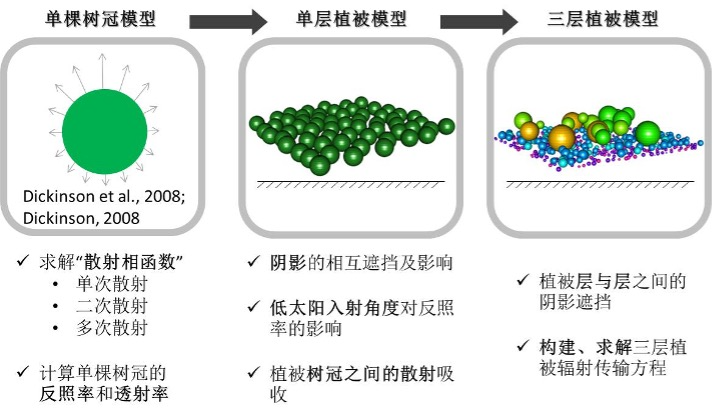
\includegraphics{Figures/辐射过程及辐射通量计算/三维植被辐射传输模型的基本框架.png}
\caption{三维植被辐射传输模型的基本框架示意图。}
\label{fig:三维植被辐射传输模型的基本框架}
\end{figure}
}


\subsection{单棵树冠模型}
单棵树冠模型基本假设是把植被树冠看成一个个的圆形球体,
叶片在其中均一分布,且叶倾角为球形分布(即$G$函数为1/2,$G$函数为单位体积叶面在某方向上的平均投影面积)。
首先考虑太阳辐射垂直入射,计算单棵球形植被的直射透射率$T_{d,s}\left(\tau\right)$,
$\tau$为沿球形植被半径长度的光学厚度参数(对于单棵树冠记为$\tau_0$,图\ref{fig:单棵树冠示意图})。
{
\begin{figure}[]
\centering
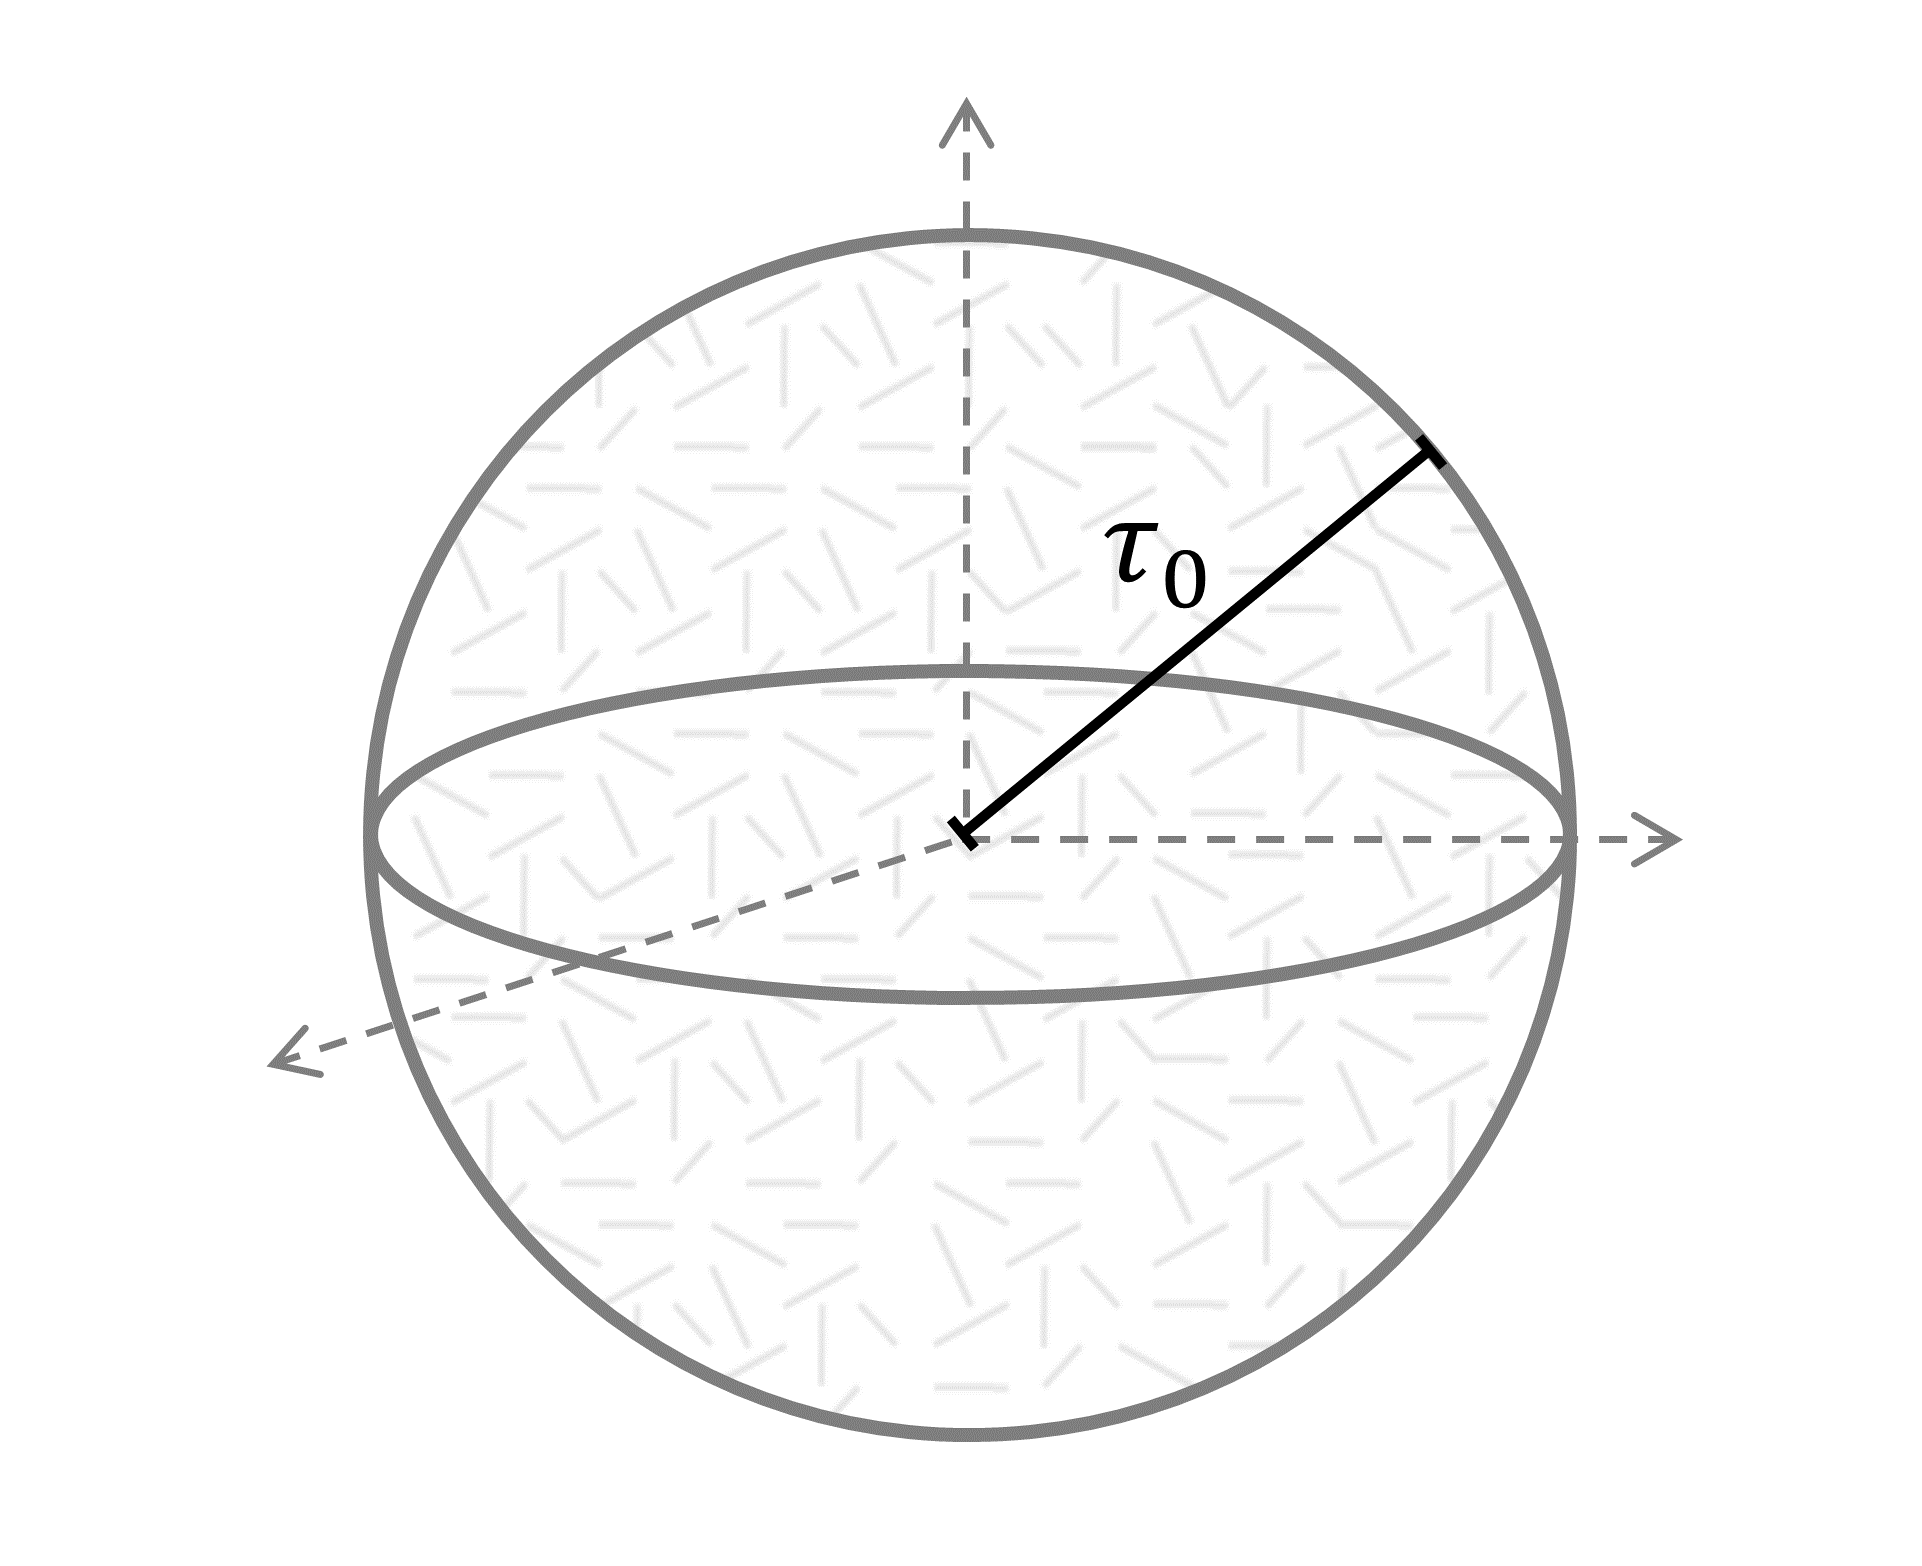
\includegraphics{Figures/辐射过程及辐射通量计算/单棵树冠示意图.png}
\caption{单棵树冠示意图。}
\label{fig:单棵树冠示意图}
\end{figure}
}


\begin{equation}\label{T_ds_tau}
T_{d, s}(\tau)=0.5 \tau^{-2}\left[1-(1+2 \tau) e^{-2 \tau}\right]
\end{equation}
对单次散射的前向、后向散射相函数($\Phi_{1f}\left(\tau\right)$,$\Phi_{1b}\left(\tau\right)$)计算为:
\begin{equation}
\Phi_{1 b}(\tau)=0.5\left[1-T_{d, s}(2 \tau)\right]
\end{equation}
\begin{equation}
\Phi_{1 f}(\tau)=\tau^{-2}\left[1-\left(1+2 \tau+2 \tau^{2}\right) e^{-2 \tau}\right]
\end{equation}
上式$\Phi_{1b}$和$\Phi_{1f}$为归一化结果(除以$0.25\omega^2/\pi$)。
二次散射前向、后向散射相函数($\Phi_{2f}\left(\tau\right),\Phi_{2b}\left(\tau\right)$)计算为:
\begin{equation}
\Phi_{2 b}(\tau)=a\left[\frac{1}{b+1}-\frac{1}{b-1} T_{d, s}(2 \tau)+\frac{2}{(b+1)(b-1)} T_{d, s}((b+1) \tau)\right]
\end{equation}
\begin{equation}
\begin{array}{c}\Phi_{2 f}(\tau)=a\left[\frac{2 b}{b^{2}-1} \Phi_{1 f}(\tau)-\left(\frac{1}{(b+1)^{2}}+\frac{1}{(b-1)^{2}}\right) T_{d, S}(\tau)+\frac{1}{(b-1)^{2}} T_{d, S}(b \tau)\right. \\ \left.\quad+\frac{1}{(b+1)^{2}} T_{d, s}((b+2) \tau)\right]\end{array}
\end{equation}
其中$a=0.70$,$b=1.74$,以上两式也为均一化的结果(除以$0.25\omega/\pi$)。假设单次和二次散射相函数从前向到后向强度线性变化,则总的单次散射和二次散射辐射计算为:
\begin{equation}
\Phi_{1 a}(\tau)=0.5\left[\Phi_{1 b}(\tau)+\Phi_{1 f}(\tau)\right]
\end{equation}
\begin{equation}
\Phi_{1 a}(\tau)=0.5\left[\Phi_{1 b}(\tau)+\Phi_{1 f}(\tau)\right]
\end{equation}
对于三次及以上散射相函数($\Phi_{3+}\left(\tau\right)$),假设其各向均一,利用二次散射后再次(与植被)碰撞的概率($p_2\left(\tau\right)$)进行计算:
\begin{equation}
\Phi_{3+}(\tau)=\frac{\omega p_{2}(\tau) \Phi_{2 a}(\tau)}{1-\omega p_{2}(\tau)}
\end{equation}
其中
\begin{equation}
p_{2}(\tau)=1-\frac{\Phi_{2 a}(\tau)}{1-T_{d, s}(\tau)-\Phi_{1 a}(\tau)}
\end{equation}
$\Phi_{3+}$为归一化结果(除以$0.25\omega^2/\pi$)。通过累加得到总的前向散射相函数($\Phi_f\left(\tau\right)$)及后向散射相函数($\Phi_b\left(\tau\right)$):
\begin{equation}
\Phi_{b}(\tau)=\frac{\omega}{4 \pi} \Phi_{1 b}(\tau)+\frac{\omega^{2}}{4 \pi}\left[\Phi_{2 b}(\tau)+\Phi_{3+}(\tau)\right]
\end{equation}
\begin{equation}
\Phi_{f}(\tau)=\frac{\omega}{4 \pi} \Phi_{1 f}(\tau)+\frac{\omega^{2}}{4 \pi}\left[\Phi_{2 f}(\tau)+\Phi_{3+}(\tau)\right]
\end{equation}
假设散射相函数的分布由后向到前向,沿天顶角呈线性变化(方位角水平均一),对任意散射出射角度$\theta_{out}$(天顶角方向,$\mu_{out}=\cos{\theta_{out}}$),其总的散射相函数计算为:
\begin{equation}
\Phi_{\mu_{\mathrm{out}}}(\tau)=\Phi_{a}(\tau)+\mu_{\mathrm{out}} \Phi_{d}(\tau)
\end{equation}
其中$\Phi_a\left(\tau\right)=0.5\left[\Phi_b\left(\tau\right)+\Phi_f\left(\tau\right)\right]$,$\Phi_d\left(\tau\right)=0.5\left[\Phi_b\left(\tau\right)-\Phi_f\left(\tau\right)\right]$。
对太阳入射天顶角为$\theta(\mu=\cos{\theta})$时,对$\Phi_{\mu_{out}}\left(\tau\right)$进行积分计算,得到单株植物的反照率($\alpha_s\left(\mu,\tau\right)$)及漫射透射率($T_{i,s}\left(\mu,\tau\right)$)为:
\begin{equation}
\alpha_{s}(\mu, \tau)=2 \pi\left[\Phi_{a}(\tau)+0.5 \mu \Phi_{d}(\tau)\right]
\end{equation}
\begin{equation}
T_{i, s}(\mu, \tau)=2 \pi\left[\Phi_{a}(\tau)-0.5 \mu \Phi_{d}(\tau)\right]
\end{equation}
对于漫射辐射入射,模型考虑等效为直射入射为60$\deg$时的情形。
\subsection{单层植被模型}
单层植被模型假设球形树冠在水平方向上随机分布,但垂直投影不重叠。在植被覆盖率为$f_c$时,不考虑重叠的植被阴影面积为:
\begin{equation}
S_{0}=f_{c} / \mu
\end{equation}
若植被树冠的阴影可以随机重叠,根据概率理论模型,可以计算阴影面积为$1-e^{-f_c/\mu}$。但考虑在实际中,植被树冠在垂直投影上一般不重叠,修正的阴影面积为:
\begin{equation}\label{S_area}
S=\frac{1-e^{-f_{c} / \mu}}{1-f_{c} e^{-1 / \mu}}
\end{equation}
树冠阴影的重叠不仅直接影响阴影面积的大小,还增加了辐射穿过植被冠层的光学路径,单层植被的光学厚度把原有的单株植物光学厚度$\tau_0$等效修改为:
\begin{equation}\label{tau}
\tau=\tau_{0} S_{0} / S
\end{equation}
随着$f_c$的增加,植被树冠之间的散射吸收增加,为了计算这部分辐射,考虑最为简单的正六边形植被树冠分布(图\ref{fig:散射吸收计算示意图}),容易计算得到红色树冠相对于绿色树冠的可视因子为:
\begin{equation}
V_{1}=\frac{1}{2}\left(1-\cos \theta_{v}\right)=\frac{1}{2}\left[1-\sqrt{1-\left(\frac{R}{L_{1}}\right)^{2}}\right]
\end{equation}
其中$\left(\frac{R}{L_{1}}\right)^{2}=\frac{\sqrt{3} f_{c}}{2 \pi}$。
考虑中心球周围6个树冠及稍远6个树冠对其散射辐射的吸收,可以得到总的可视因子为:
\begin{equation}
V=6 V_{1}+6 V_{2}=3\left[1-\sqrt{1-\frac{\sqrt{3} f_{c}}{2 \pi}}\right]+3\left[1-\sqrt{1-\frac{\sqrt{3} f_{c}}{6 \pi}}\right]
\end{equation}
假设可视立体角(在各个方位角方向)均一分布在中心球形树冠平行于地面的大圆上下$\pm\mu_v$的角度范围内,于是$\mu_v=V$。对球形树冠的散射相函数进行积分得到初次拦截的散射辐射为
\begin{equation}
\frac{1}{2 \pi} \int_{0}^{2 \pi} \int_{-\mu_{v}}^{\mu_{v}} 2 \pi\left(\Phi_{a}+\mu \Phi_{d}\right) d \mu d \phi=4 \pi V \Phi_{a}
\end{equation}
利用再次碰撞概率概念估算总的树冠之间散射吸收为
\begin{equation}
A_{c}=4 \pi V \Phi_{a}\left(\tau_{0}\right)\left[1-T_{d, s}\left(\tau_{0}\right)\right] \frac{1-\omega}{1-\omega p_{2}\left(\tau_{0}\right)}
\end{equation}
其中$\omega$为叶片单次散射反照率。

{
\begin{figure}[]
\centering
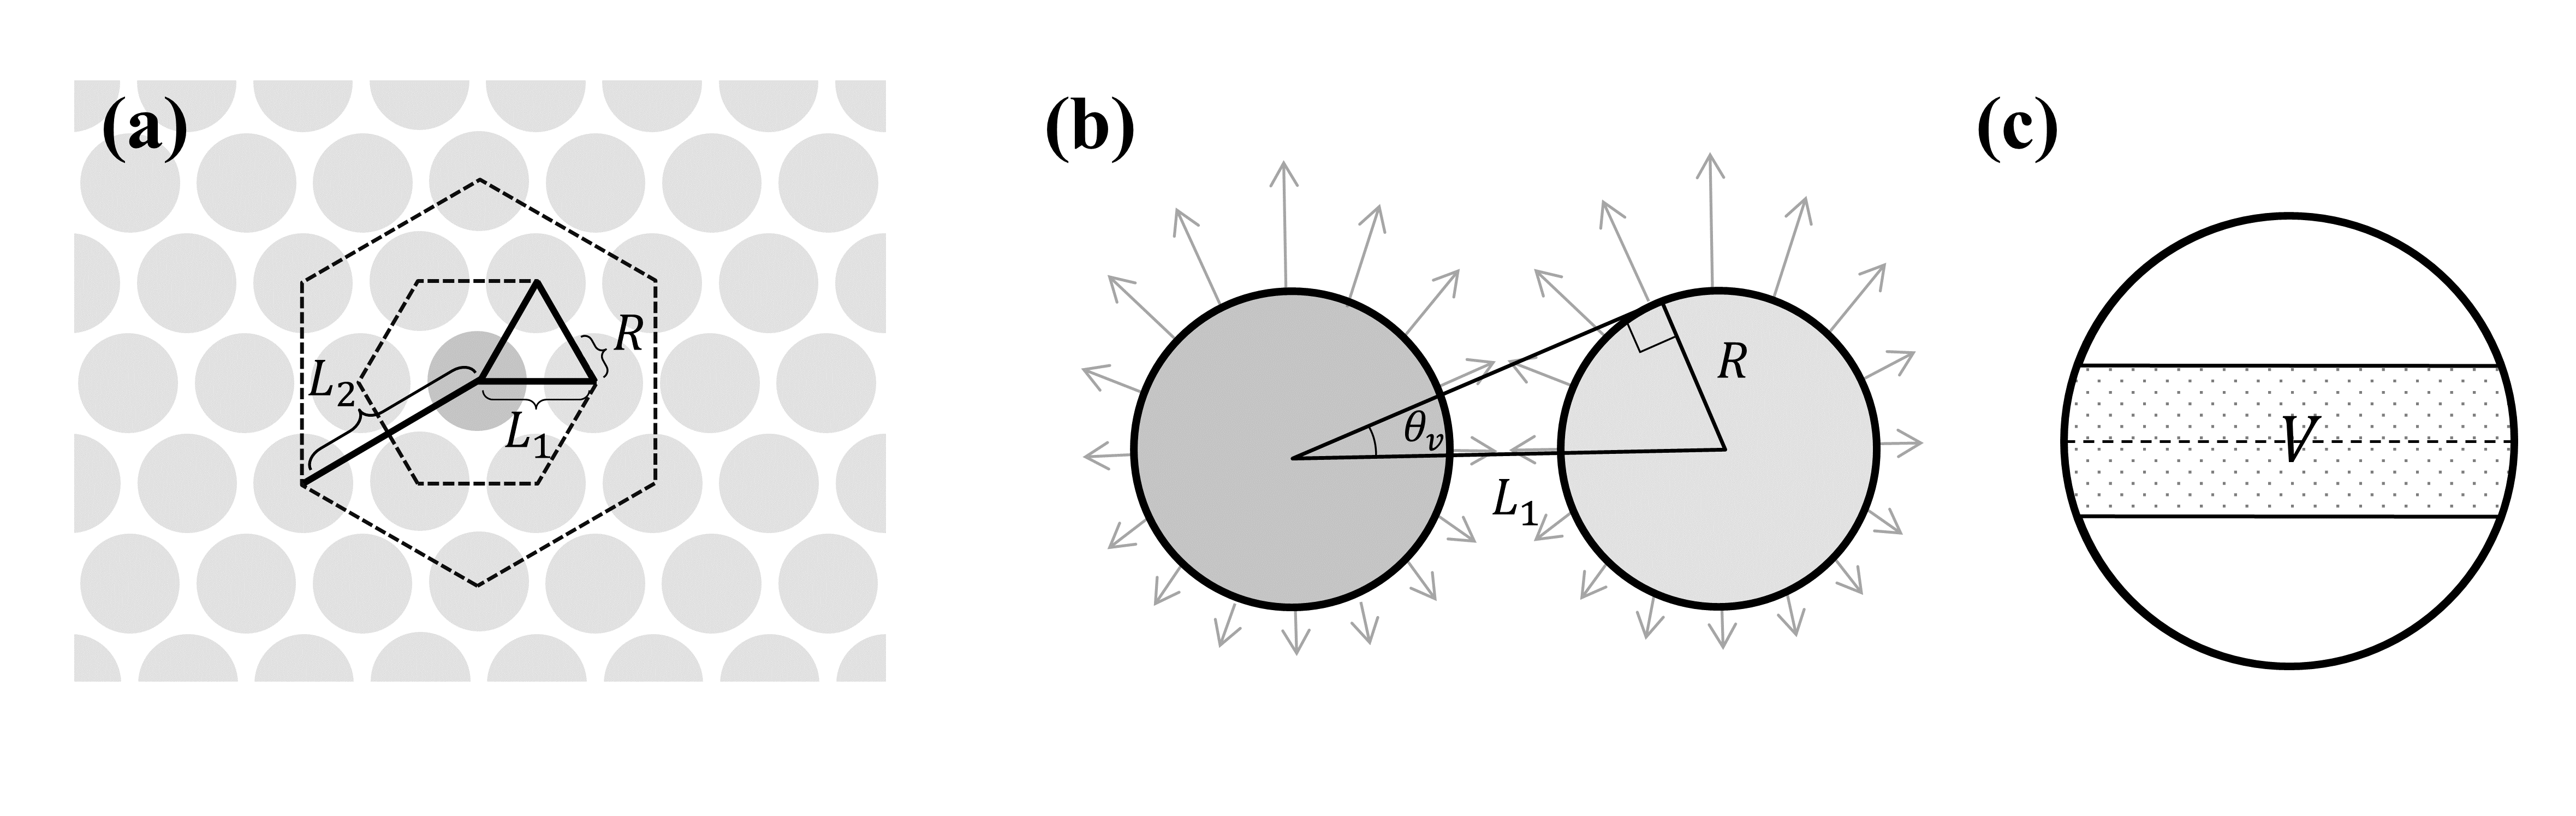
\includegraphics{Figures/辐射过程及辐射通量计算/散射吸收计算示意图.png}
\caption{植被树冠之间散射吸收计算示意图。}
\label{fig:散射吸收计算示意图}
\end{figure}
}

当太阳在较低的角度(高度角)入射时,植被树冠阴影重叠概率增大,树冠的光照面主要集中在顶部,此时的植被冠层类似于一维的情形,相对于球形植被计算结果,$albedo$会有所增加。
我们利用 \citet{dickinson1983land} 年对一维植被单次散射的分析结果,计算对$albedo$的增量为:
\begin{equation}
\alpha_{L}=(N-1) \alpha_{s}\left(\mu=1, \tau_{0}\right) f_{c}\left(\frac{1}{s}-\frac{1}{s_{0}}\right)
\end{equation}
其中$N$表示相对于垂直入射植被冠层时$albedo$的倍数,是太阳入射角度的函数:
\begin{equation}
N=\frac{1+2 \beta_{2}}{1+2 \beta_{2} \mu}
\end{equation}
其中$\beta_2=\left(1-\omega\right)^\frac{1}{2}(1-\omega+2\omega\beta)$。
植被树冠之间的吸收增量会使$albedo$和漫射透射减少,低入射角度对$albedo$的增量会降低植被的吸收和漫射透射,把以上增加的部分均一分配到减少项,
得到单层植被$albedo$($\alpha$),植被直射透射($T_d$)漫射透射($T_i$)及吸收($A$)为
\begin{equation}
\alpha=\alpha_{s}(\mu, \tau)+\alpha_{L}-0.5 A_{c}
\end{equation}
\begin{equation}
T_{i}=T_{i, s}(\mu, \tau)-0.5 \alpha_{L}-0.5 A_{c}
\end{equation}
\begin{equation}
A=1-\alpha-T_{i}-T_{d}
\end{equation}
对于漫射辐射入射,同样考虑等效为直射入射为60$^\circ$的情形。
以上的推导均基于正球体和球形叶倾角分布函数情况下。对于椭球体树冠(图\ref{fig:椭球体树冠} a),其对辐射计算的影响主要有3个方面(均可等效看成对光学厚度$\tau$的影响):
\begin{enumerate}
    \item 椭球相对于正球的拉升/压缩影响单位长度的光学厚度(因叶密度改变);
    \item 几何形状的改变造成光学路径的长度的改变;
    \item 阴影面积重合部分改变对光学厚度的影响。
\end{enumerate}

 {
    \begin{figure}[]
    \centering
    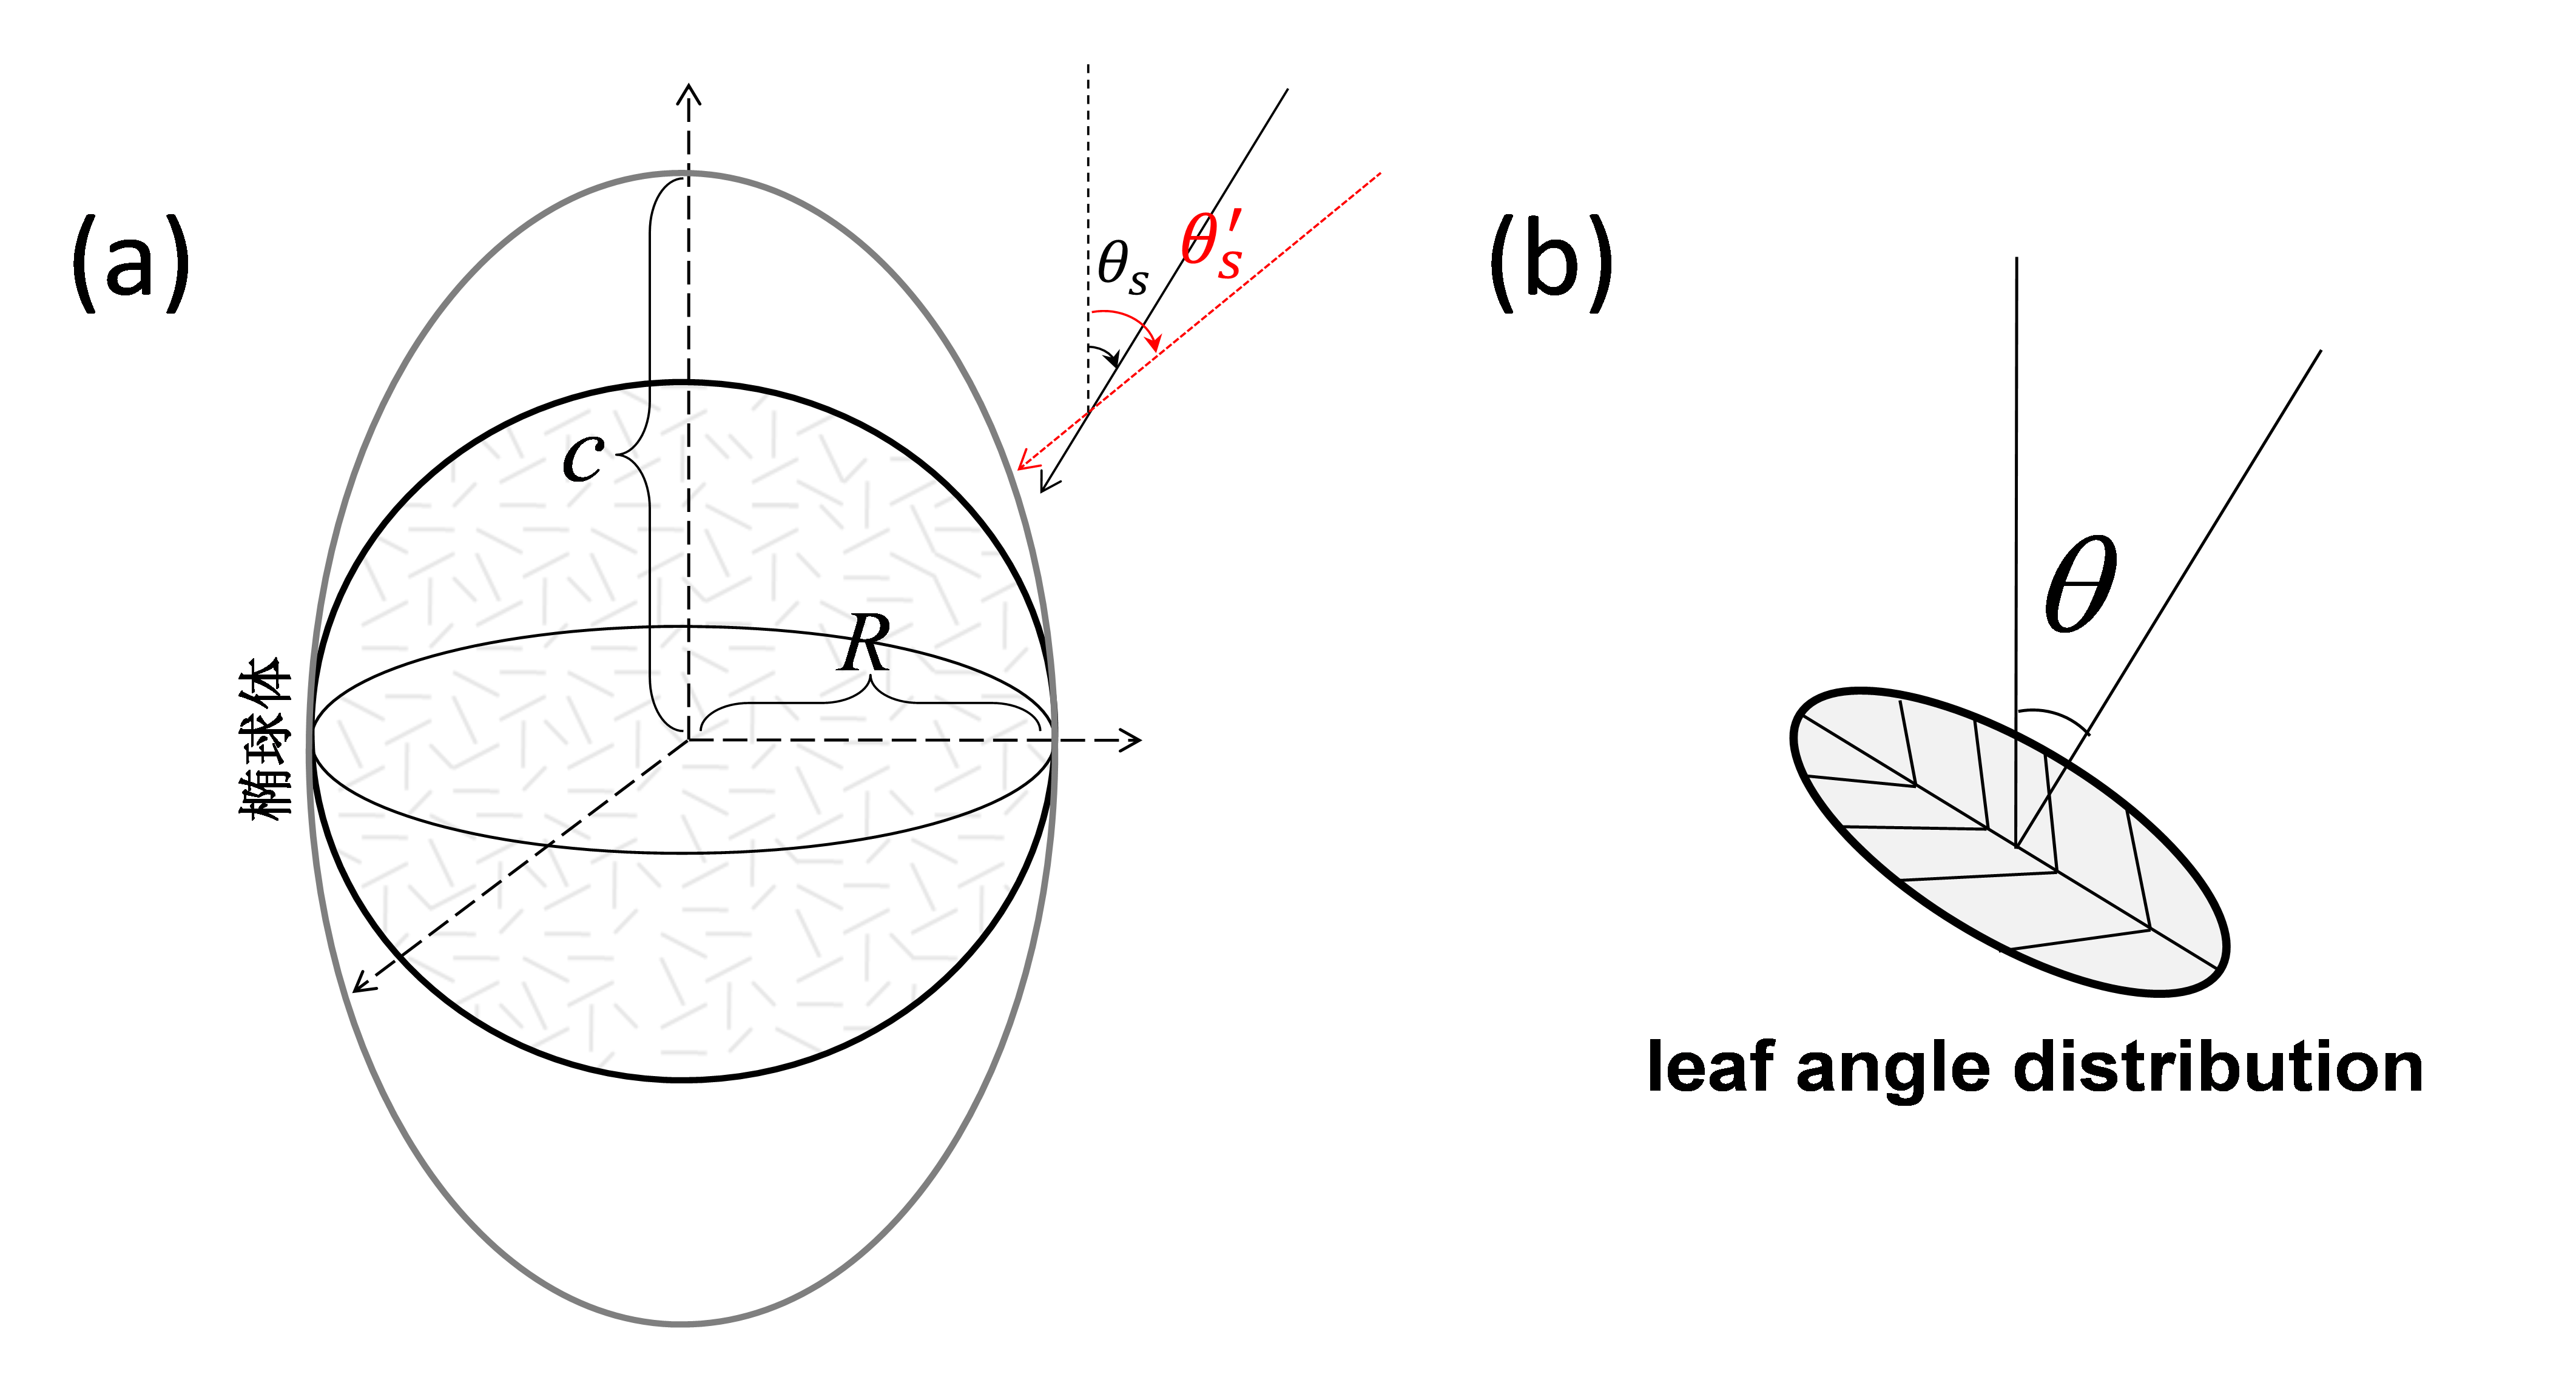
\includegraphics{Figures/辐射过程及辐射通量计算/椭球体树冠.png}
    \caption{(a) 树冠形状从正球体扩展到椭球体;(b) 考虑叶倾角分布。}
    \label{fig:椭球体树冠}
    \end{figure}
    }
    

椭球体可能看成是正球体在垂直方向$y$轴的拉伸,在椭球坐标系下的$y$,
在正球体坐标系下就变成$y\prime$。让$c$为椭球体半轴长(沿$y$轴),$R$为球体水平方向的半径,可以得到
\begin{equation}
y^{\prime}=\frac{R}{c} y, \text { and } x^{\prime}=x
\end{equation}
于是有$\tan{\theta_s^\prime}=\frac{x^\prime}{y^\prime}=\frac{c}{R}{\tan{\theta}}_s$,
椭球体在地面的投影面积即为$\pi R^2/\cos{\theta_s^\prime}$。将$\theta_s^\prime$进行替换,得到阴影面积计算公式为
\begin{equation}\label{SSS}
\begin{aligned} S &=\frac{\pi R^{2}}{\cos \theta_{s}^{\prime}} \\ &=\frac{\pi R^{2}}{\cos \theta_{s} 
\sqrt{\frac{1}{c r^{2} \sin ^{2} \theta_{s}+\cos ^{2} \theta_{s}}}} \end{aligned}
\end{equation}
式中$cr=c/R$。可以看出,当$c=R$时,与正球体计算一致。$\cos{\theta_s}$与$\cos{\theta_s^\prime}$的关系从公式 (\ref{SSS}) 很容易看出。%caution


椭球体对$\tau$影响的三个方面,我们用$c1$, $c2$, $c3$三个系数表示。对于$c1$,很容易得到$c1=1/cr$。$c2$的计算稍微复杂一点,可表达为
\begin{equation}
\begin{aligned} c 2 &=\frac{y}{y^{\prime}} \cdot \frac{\cos \theta_{s}^{\prime}}{\cos \theta_{s}}=
    c r \sqrt{\frac{1}{c r^{2} \sin ^{2} \theta_{s}+\cos ^{2} \theta_{s}}} \\ &=
    \sqrt{\frac{c^{2}}{c^{2} \sin ^{2} \theta_{s}+R^{2} \cos ^{2} \theta_{s}}} \end{aligned}
\end{equation}
对于$c3$,实际上是计算在等效的天顶角$\theta_s^\prime$下,考虑阴影重叠后的等效$\tau$,其计算表达式在公式(\ref{tau})已给出。


对于球形分布函数,前面已提到$G=0.5$;对于参数为$\chi_L$的叶倾角分布,
可以利用公式(\ref{Gmu})计算得到特定太阳入射角的$G\left(\theta_s\right)$。
对于光学厚度相对原始$\tau$的比例系数为$c4=G\left(\theta_s\right)/0.5$。


综合以上几个方面,即把光学厚度参数$\tau$修改为$c1c2c3c4\tau$,
然后代入直射透射计算公式,便可得到单层植被的直射透射率$T_d^\prime$,
假设在正球体情况下的直射透射率为$T_d$,在不考虑椭球形状和叶倾角分布情况下,能量守恒等式表达为
\begin{equation}
\alpha+A+T_{d}+T_{i}=1
\end{equation}
定义散射/吸收辐射的订正因子为$\frac{1-T_d^\prime}{1-T_d}$,把由直射透射引起的截获辐射量变化考虑为$S$和$A$的改变,
即分别修正为$\frac{1-T_d^\prime}{1-T_d}S$和$\frac{1-T_d^\prime}{1-T_d}A$,新修正的各个变量同样满足能量守恒方程
\begin{equation}
\frac{1-T_{d}^{\prime}}{1-T_{d}} \alpha+\frac{1-T_{d}^{\prime}}{1-T_{d}} A+T_{d}^{\prime}+\frac{1-T_{d}^{\prime}}{1-T_{d}} T_{i}=1
\end{equation}
再考虑对单层植被辐射散射/吸收特性的改变之外,树冠的形状改变还影响地面的阴影计算,对于单层植被,
可以利用等效的$\cos{\theta_s^\prime}$值(即$\cos{\theta_s}\sqrt{\frac{1}{{cr}^2\sin^2{\theta_s}+\cos^2{\theta_s}}}$)。 
若考虑植被与地面之间的多次散射,初次透射到地面的辐射$T$($T=1-S+S\left(T_d+T_i\right)$)经过地面的反射(地表反射率$r_g$),再次与植被冠层反射到达地面,
如此反复。到达地面的辐射为一等比数列,其比例因子为$q=r_gS^\ast\alpha^\ast$,上标“$\ast$”表示漫射辐射入射时相应变量值(下同)。
由于地表与植被之间多次散射的植被吸收$A^m=\frac{Tr_gS^\ast A^\ast}{1-q}$,
总的植被吸收($\left[A\right]$),透射率($\left[T\right]$),地表吸收($\left[G\right]$)和地表$albedo$($\left[\alpha\right]$)计算如下
\begin{equation}
[A]=S A+A^{m}
\end{equation}
\begin{equation}
[T]=\frac{T}{1-q}
\end{equation}
\begin{equation}
[G]=\left(1-r_{g}\right)[T]
\end{equation}
\begin{equation}
[\alpha]=1-[A]-[G]
\end{equation}
\subsection{三层植被模型}
三层植被模型的假设在单株植物模型和单层植被模型的基础上,认为层与层之间的树冠垂直投影不重叠,
每层植被树冠半径$(R$)和树冠中心高度($h$)相同(图\ref{fig:三层植被结构示意图})。
若某层植被含有多种PFT,则该层的$f_c$为所含PFT各自$f_c$的累加,
植被参数的层属性(包括$LAI$、$R$、$h$及叶片光学属性)为所含PFT的$f_c$加权平均。



层与层之间的阴影重叠对直射辐射的吸收影响很大,特别是对于较高吸收率的可见光波段。
对于阴影的重叠,3D模型假设高层树冠的“自身阴影”(在低层植被的阴影与其自身垂直投影的重叠区域)
不与低层树冠的阴影重叠(如图\ref{fig:三层植被结构示意图}所示的$S_{12}$、$S_{13}$和$S_{23}$)。除此之外,层与层之间的阴影可以随机重叠。
{
\begin{figure}[]
\centering
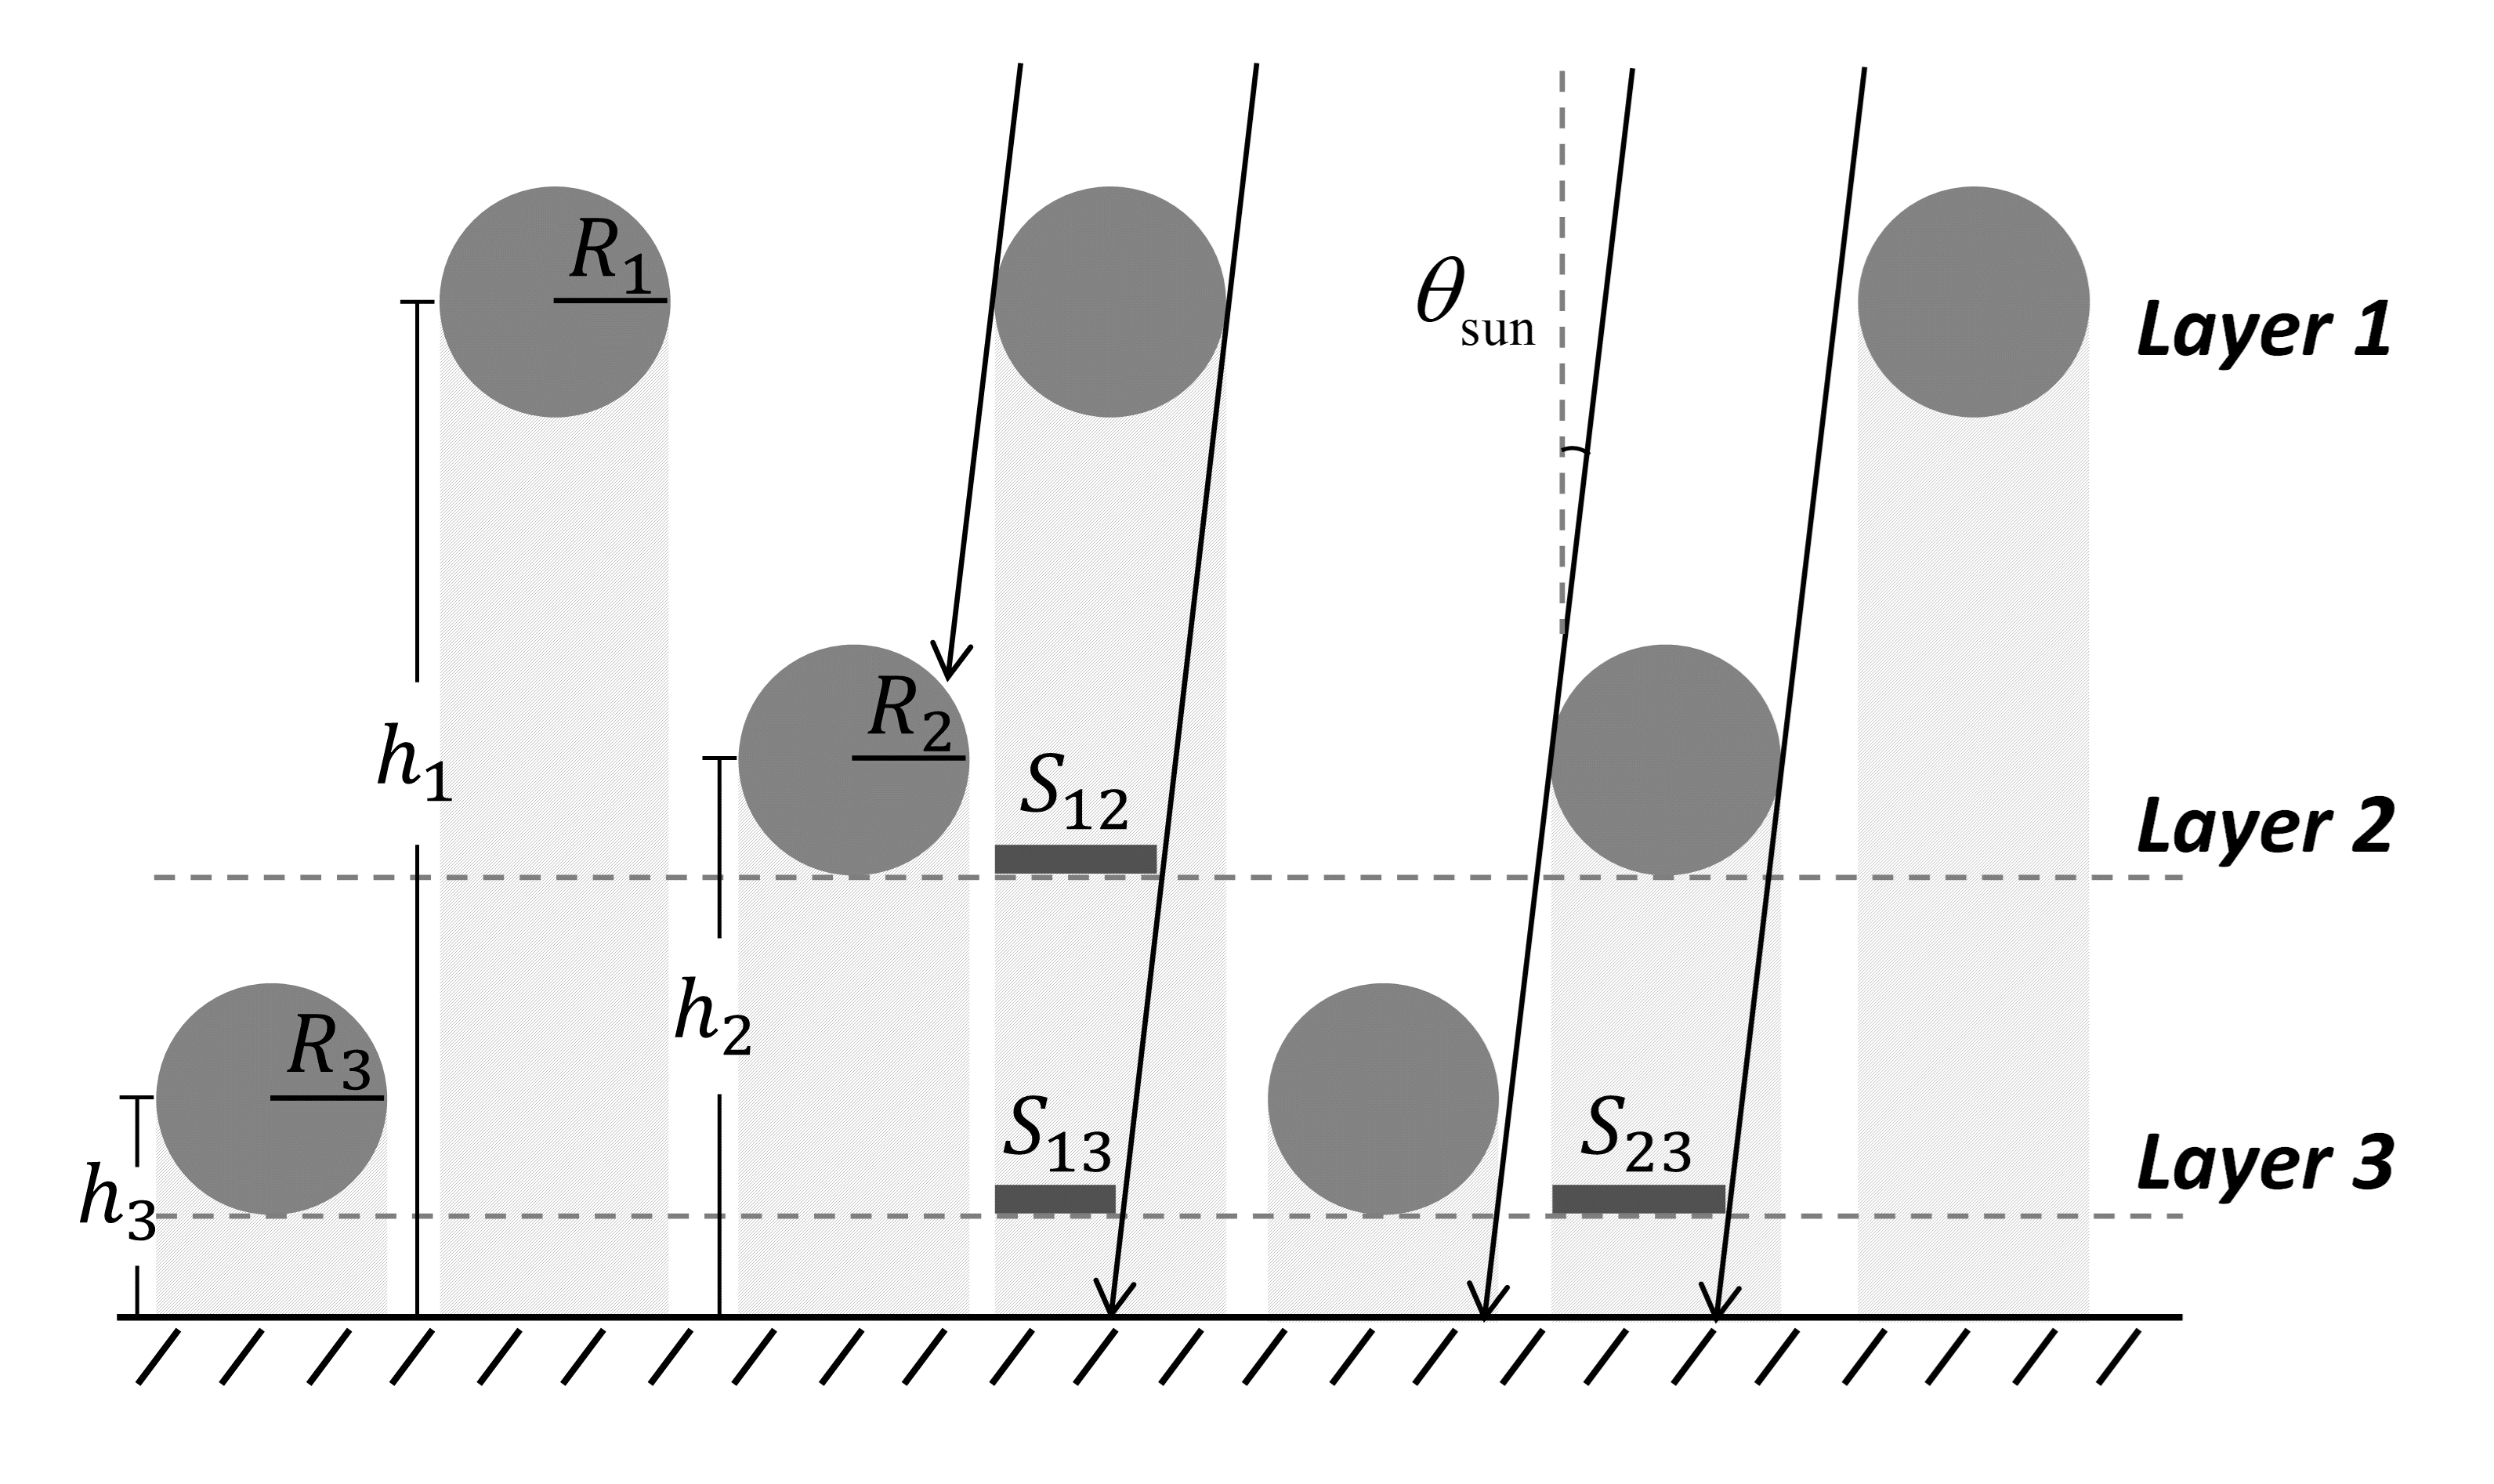
\includegraphics{Figures/辐射过程及辐射通量计算/三层植被结构示意图.png}
\caption{三层植被结构示意图。}
\label{fig:三层植被结构示意图}
\end{figure}
}
用$I_{\left[from\right]\rightarrow\left[to\right]}$表示层与层之间的直射辐射直射透射量,
$S[n]$表示第$n$层植被的阴影面积,$Td$,$[n]$为第$n$层植被的直射辐射直射透射率,可以计算从天空($sky$),
不穿过植被,到达每层植被及地面的初始直射辐射为(为了与三维植被辐射传输模型引文 \citep{yuan20143d} 吻合
,这里保留了植被分层计数从上到下1-3的方式,但之后三维植被长波辐射传输
、三维植被湍流交换过程等采用从上至下3-1的编号,与代码一致。) :
\begin{equation}
\begin{aligned} I_{0 \rightarrow 1} &=S_{1} \\ I_{0 \rightarrow 2} &=\left(1-S_{1}+S_{12}\right) S_{2} \\ 
    I_{0 \rightarrow 3} &=\left[1-\left(S_{1}-S_{13}\right)-\left(S_{2}-S_{23}\right)+\left(S_{1}-S_{12}\right)\left(S_{2}-S_{23}\right)\right] S_{3} \\ 
    I_{0 \rightarrow g} &=1-S_{1}-S_{2}-S_{3} \\ &+\left(S_{1}-S_{12}\right) S_{2}+\left(S_{1}-S_{13}\right) S_{3}+\left(S_{2}-S_{23}\right) S_{3} \\
     &-\left(S_{1}-S_{12}\right)\left(S_{2}-S_{23}\right) S_{3} \end{aligned}
\end{equation}
到达L1的直射辐射可以继续直射透射到达下层,计算为:
\begin{equation}
\begin{array}{l}I_{1 \rightarrow 2}=T_{d, 1}\left(S_{1}-S_{12}\right) S_{2} \\
     I_{1 \rightarrow 3}=T_{d, 1}\left[S_{1}-S_{13}-\left(S_{1}-S_{12}\right)\left(S_{2}-S_{23}\right)\right] S_{3} \\
      I_{1 \rightarrow g}=T_{d, 1}\left[S_{1}-\left(S_{1}-S_{12}\right) S_{2}-\left(S_{1}-S_{13}\right) S_{3}+\left(S_{1}-S_{12}\right)\left(S_{2}-S_{23}\right) S_{3}\right]\end{array}
\end{equation}
同理可以得到:
\begin{equation}
\begin{array}{l}I_{2 \rightarrow 3}=T_{d, 2}\left[I_{0 \rightarrow 2}+I_{1 \rightarrow 2}\right] \frac{\left(S_{2}-S_{23}\right) S_{3}}{S_{2}} \\
     I_{2 \rightarrow g}=T_{d, 2}\left[I_{0 \rightarrow 2}+I_{1 \rightarrow 2}\right] \frac{S_{2}-\left(S_{2}-S_{23}\right) S_{3}}{S_{2}} \\ 
     I_{3 \rightarrow g}=T_{d, 3}\left[I_{0 \rightarrow 3}+I_{1 \rightarrow 3}+I_{2 \rightarrow 3}\right]\end{array}
\end{equation}

累加以上结果,可以计算到达每层的初始直射辐射为:
\begin{equation}
\begin{array}{l}I_{1}=I_{0 \rightarrow 1} \\ I_{2}=I_{0 \rightarrow 2}+I_{1 \rightarrow 2} \\ 
    I_{3}=I_{0 \rightarrow 3}+I_{1 \rightarrow 3}+I_{2 \rightarrow 3} \\ 
    I_{g}=I_{0 \rightarrow g}+I_{1 \rightarrow g}+I_{2 \rightarrow g}+I_{3 \rightarrow g}\end{array}
\end{equation}
第n层植被的直射辐射直射吸收量为:
\begin{equation}
I_{n}\left(1-T_{d, n}\right)(1-\omega)
\end{equation}
第n层植被的太阳直射照射面积($p_{sun}$)计算为:
\begin{equation}
P_{\mathrm{sun}}=I_{n} / S_{n}
\end{equation}
上式表明每层植被并不是100\%的被太阳直射照射,该参数将会用于修正植被光照叶面积指数(图 \ref{fig:三层植被辐射传输计算示意图})。
{
\begin{figure}[]
\centering
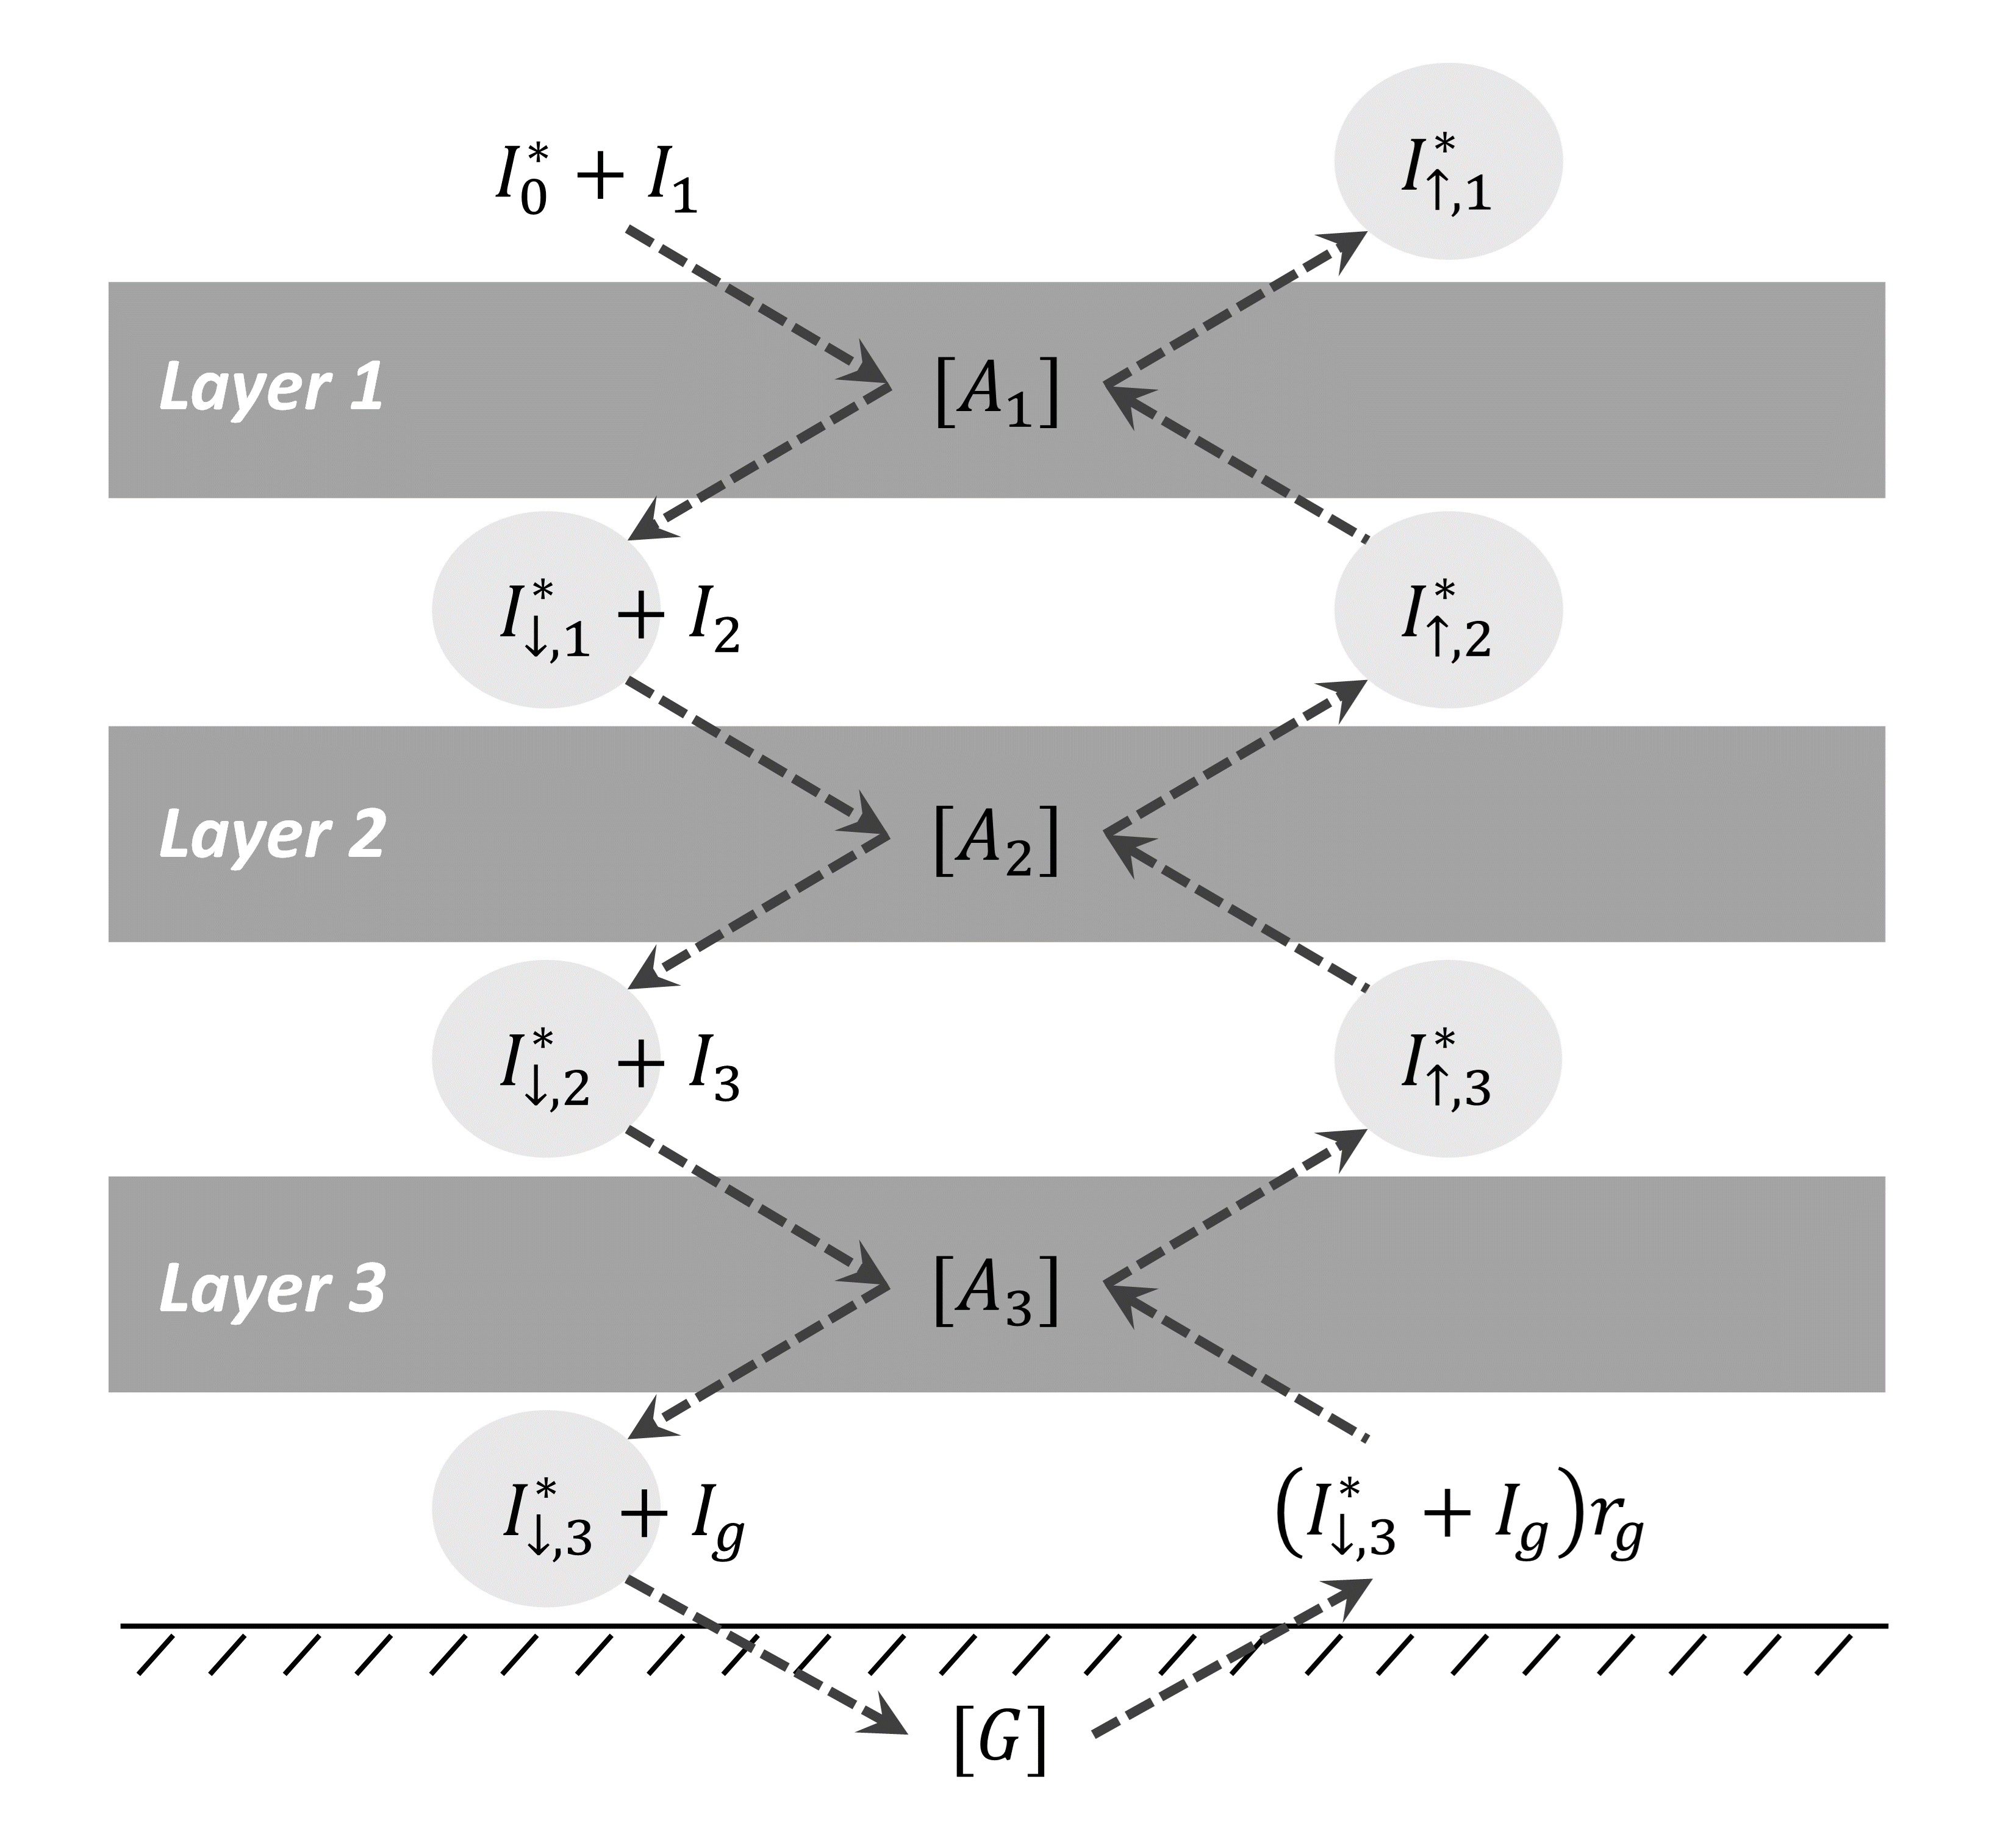
\includegraphics{Figures/辐射过程及辐射通量计算/三层植被辐射传输计算示意图.png}
\caption{三层植被辐射传输计算示意图。}
\label{fig:三层植被辐射传输计算示意图}
\end{figure}
}
三层植被模型的计算采用线性方程组进行计算。六个变量,$I_{\uparrow,1}^\ast$, $I_{\downarrow,1}^\ast$, $I_{\uparrow,2}^\ast$, $I_{\downarrow,2}^\ast$, $I_{\uparrow,3}^\ast$ 和 $I_{\downarrow,3}^\ast$,
被选择作为未知变量。他们分别表示每层植被的向上/向下漫射辐射通量,可以表示为
\begin{equation}
\begin{array}{l}I_{\uparrow, 1}^{*}=I_{1} \alpha_{1}+I_{\uparrow, 2}^{*} S_{1}^{*} T_{i, 1}^{*}+I_{\uparrow, 2}^{*}\left(1-S_{1}^{*}\right)+I_{0}^{*} S_{1}^{*} \alpha_{1}^{*} 
    \\ I_{\downarrow, 1}^{*}=I_{1} T_{i, 1}+I_{0}^{*} S_{1}^{*} T_{i, 1}^{*}+I_{0}^{*}\left(1-S_{1}^{*}\right)+I_{\uparrow, 2}^{*} S_{1}^{*} \alpha_{1}^{*} 
    \\ I_{\uparrow, 2}^{*}=I_{2} \alpha_{2}+I_{\uparrow, 3}^{*} S_{2}^{*} T_{i, 2}^{*}+I_{\uparrow, 3}^{*}\left(1-S_{2}^{*}\right)+I_{\downarrow, 1}^{*} S_{2}^{*} \alpha_{2}^{*}
     \\ I_{\downarrow, 2}^{*}=I_{2} T_{i, 2}+I_{\downarrow, 1}^{*} S_{2}^{*} T_{i, 2}^{*}+I_{\downarrow, 1}^{*}\left(1-S_{2}^{*}\right)+I_{\uparrow, 3}^{*} S_{2}^{*} \alpha_{2}^{*} 
     \\ I_{\uparrow, 3}^{*}=I_{3} \alpha_{3}+\left(I_{\downarrow, 3}^{*}+I_{g}\right) r_{g} S_{3}^{*} T_{i, 3}^{*}+\left(I_{\downarrow, 3}^{*}+I_{g}\right) r_{g}\left(1-S_{3}^{*}\right)+I_{\downarrow, 2}^{*} S_{3}^{*} \alpha_{3}^{*} 
     \\ I_{\downarrow, 3}^{*}=I_{3} T_{i, 3}+I_{\downarrow, 2}^{*} S_{3}^{*} T_{i, 3}^{*}+I_{\downarrow, 2}^{*}\left(1-S_{3}^{*}\right)+\left(I_{\downarrow, 3}^{*}+I_{g}\right) r_{g} S_{3}^{*} \alpha_{3}^{*}\end{array}
\end{equation}
经过简单的变换,可以得到在直射入射辐射情况下:
\begin{equation}
\left(\begin{matrix}1&&-{\widetilde{T}}_1&&&\\&1&-{\widetilde{\alpha}}_1&&&\\&-{\widetilde{\alpha}}_2&1&&-{\widetilde{T}}_2&\\&-{\widetilde{T}}_2&&1&-{\widetilde{\alpha}}_2&\\&&&-{\widetilde{\alpha}}_3&1&-{\widetilde{T}}_3r_g\\&&&-{\widetilde{T}}_3&&1-r_g{\widetilde{\alpha}}_3\\\end{matrix}\right)\left(\begin{matrix}I_{\uparrow,1}^\ast\\I_{\downarrow,1}^\ast\\I_{\uparrow,2}^\ast\\I_{\downarrow,2}^\ast\\I_{\uparrow,3}^\ast\\I_{\downarrow,3}^\ast\\\end{matrix}\right)=\left(\begin{matrix}I_1\alpha_1\\I_1T_{i,1}\\I_2\alpha_2\\I_2T_{i,2}\\I_3\alpha_3+I_gr_g{\widetilde{T}}_3\\I_3T_{i,3}+I_gr_g{\widetilde{\alpha}}_3\\\end{matrix}\right)
\end{equation}
及在漫射辐射情况下:
\begin{equation}
\left(\begin{matrix}1&&-{\widetilde{T}}_1&&&\\&1&-{\widetilde{\alpha}}_1&&&\\&-{\widetilde{\alpha}}_2&1&&-{\widetilde{T}}_2&\\&-{\widetilde{T}}_2&&1&-{\widetilde{\alpha}}_2&\\&&&-{\widetilde{\alpha}}_3&1&-{\widetilde{T}}_3r_g\\&&&-{\widetilde{T}}_3&&1-r_g{\widetilde{\alpha}}_3\\\end{matrix}\right)\left(\begin{matrix}I_{\uparrow,1}^\ast\\I_{\downarrow,1}^\ast\\I_{\uparrow,2}^\ast\\I_{\downarrow,2}^\ast\\I_{\uparrow,3}^\ast\\I_{\downarrow,3}^\ast\\\end{matrix}\right)=\left(\begin{matrix}I_0^\ast{\widetilde{\alpha}}_1\\I_0^\ast{\widetilde{T}}_1\\0\\0\\0\\0\\\end{matrix}\right)
\end{equation}
其中${\widetilde{\alpha}}_n=S_n^\ast\alpha_n^\ast$及${\widetilde{T}}_n=S_n^\ast T_n^\ast-S_n^\ast+1$。以上两个方程组可以合并写为:
\begin{equation}
\mathbf{A X}=\mathbf{B}
\end{equation}
有很多方法去解以上方程组,根据方程组的特点,采用经过修改后的高斯消去法。对于直射入射辐射,其解为:
\begin{equation}
\begin{array}{l}{[\alpha]=I_{\uparrow, 1}^{*}} \\ {\left[A_{1}\right]=I_{1} A_{1}+I_{\uparrow, 2}^{*} S_{1}^{*} A_{1}^{*}} \\ {\left[A_{2}\right]=I_{2} A_{2}+\left(I_{\downarrow, 1}^{*}+I_{\uparrow, 3}^{*}\right) S_{2}^{*} A_{2}^{*}} \\ {\left[A_{3}\right]=I_{3} A_{3}+\left[I_{\downarrow, 2}^{*}+\left(I_{g}+I_{\downarrow, 3}^{*}\right) r_{g}\right] S_{3}^{*} A_{3}^{*}} \\ {[G]=\left(I_{g}+I_{\downarrow, 3}^{*}\right)\left(1-r_{g}\right)}\end{array}
\end{equation}
对于漫射入射,其解为:
\begin{equation}
\begin{array}{l}{\left[\alpha^{*}\right]=I_{\uparrow, 1}^{*}} \\ {\left[A_{1}^{*}\right]=S_{1}^{*} A_{1}^{*}+I_{\uparrow, 2}^{*} S_{1}^{*} A_{1}^{*}} \\ {\left[A_{2}^{*}\right]=\left(I_{\downarrow, 1}^{*}+I_{\uparrow, 3}^{*}\right) S_{2}^{*} A_{2}^{*}} \\ {\left[A_{3}^{*}\right]=\left(I_{\downarrow, 2}^{*}+I_{\downarrow, 3}^{*} r_{g}\right) S_{3}^{*} A_{3}^{*}} \\ {\left[G^{*}\right]=I_{\downarrow, 3}^{*}\left(1-r_{g}\right)}\end{array}
\end{equation}
所有的PFT(包括裸土)共享同样的反照率,同样的地面吸收率。对每一PFT,考虑其单独存在时,利用单层植被模型计算其吸收,
并将其作为权重,把每层的植被辐射吸收分配到其所包含的PFT中去(包括上面计算的直射辐射直射吸收)。

\subsection{三维植被长波辐射传输}\label{三维植被长波辐射传输}
为了说明三维植被情况下长波辐射传输与一维情况下最大的不同,我们举一个极端的例子加以说明,如图\ref{fig:单颗树冠长波辐射传输示意图}所示:
{
\begin{figure}[]
\centering
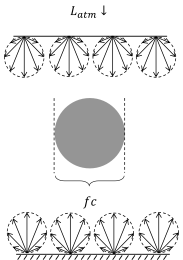
\includegraphics{Figures/辐射过程及辐射通量计算/单颗树冠长波辐射传输示意图.png}
\caption{三维长波辐射计算示意图(对于单棵树冠)。}
\label{fig:单颗树冠长波辐射传输示意图}
\end{figure}
}

若采用一维长波辐射传输方式进行计算,则到达地面的大气长波辐射量即为$f_c\left(1-\varepsilon_v\right)\\L_{atm}\downarrow+\left(1-f_c\right)L_{atm}\downarrow$。
但实际上,由于长波辐射是朝各个方向发射的,一般认为各向均一,能到达树冠表面(或称为阴影)的长波辐射并不仅仅限于其正上方的部分,
简单的计算公式可以表示为:
\begin{equation}
S=\int_{2 \pi} \frac{\cos \theta}{\pi} \cdot \frac{f_{c}}{\cos \theta} \cdot d \Omega=2 f_{c}
\end{equation}
上式中$\cos{\theta}/\pi$为入射角度为$\theta$时的辐射强度,$f_c/\cos{\theta}$为此时的树冠阴影面积(地面投影),
总的阴影面积计算为$2f_c$。到达地面的大气长波辐射量即为:
\begin{equation}
S\left(1-\varepsilon_{v}\right) L_{atm} \downarrow+(1-S) L_{atm} \downarrow
\end{equation}
与一维不同之处是$f_c$替换成了$S$。当植被比较稀疏时,
$f_c\rightarrow0$,$S\rightarrow2$,同上述单棵树冠情况一样;
当植被比较致密时,$f_c\rightarrow1$,$S\rightarrow1$,同一维情形。
对从地面发射的长波辐射,其情况同向下大气长波辐射一样,在稀疏情况下,植被能截获更多的长波辐射。
下面我们对一层植被(植被覆盖度为$f_c$)进行整个长波辐射传输过程推导。植被冠层下的长波辐射计算为:
\begin{equation}
\begin{aligned} L_{v} \downarrow &=S\left(1-\varepsilon_{v}\right) L_{atm} \downarrow+(1-S) L_{atm} \downarrow+f_{c} 
    \varepsilon_{v} \sigma T_{v}^{4} \\ &=\left(S-S \varepsilon_{v}+1-S\right) L_{atm} \downarrow+f_{c} \varepsilon_{v} 
    \sigma T_{v}^{4} \\ &=\left(1-S \varepsilon_{v}\right) L_{atm} \downarrow+f_{c} \varepsilon_{v} \sigma T_{v}^{4} \end{aligned}
\end{equation}
土壤向上的长波辐射(包括自身发射和反射部分)计算为:
\begin{equation}
L_{g} \uparrow=\left(1-\varepsilon_{g}\right) L_{v} \downarrow+\varepsilon_{g} \sigma T_{g}^{4}
\end{equation}
土壤的净长波辐射为(向上记为+):
\begin{equation}
\overrightarrow{L_{g}}=-\varepsilon_{g} L_{v} \downarrow+\varepsilon_{g} \sigma T_{g}^{4}
\end{equation}
\begin{equation}
\begin{aligned} \overrightarrow{L_{v}} &=-S \varepsilon_{v} L_{atm} \downarrow-S \varepsilon_{v} L_{g} 
    \uparrow+2 f_{c} \varepsilon_{v} \sigma T_{v}^{4} \\ &=-S \varepsilon_{v} L_{atm} \downarrow-S 
    \varepsilon_{v}\left(1-\varepsilon_{g}\right)\left(1-S \varepsilon_{v}\right) L_{atm} \\ & 
    \downarrow-S \varepsilon_{v}\left(1-\varepsilon_{g}\right) f_{c} \varepsilon_{v} \sigma T_{v}^{4}+S
     \varepsilon_{v} \varepsilon_{g} \sigma T_{g}^{4}+2 f_{c} \varepsilon_{v} \sigma T_{v}^{4} \\ 
     &=\left[2-S \varepsilon_{v}\left(1-\varepsilon_{g}\right)\right] f_{c} \varepsilon_{v} 
     \sigma T_{v}^{4}-S \varepsilon_{v}\left[1+\left(1-\varepsilon_{g}\right)\left(1-S \varepsilon_{v}\right)\right]
      L_{atm} \downarrow+S \varepsilon_{v} \varepsilon_{g} \sigma T_{g}^{4} \end{aligned}
\end{equation}
植被层顶向上的长波辐射计算为:
\begin{equation}
\begin{aligned} L \uparrow=&(1-S) L_{g} \uparrow+S\left(1-\varepsilon_{v}\right) L_{g} 
    \uparrow+f_{c} \varepsilon_{v} \sigma T_{v}^{4} \\=&\left(1-S \varepsilon_{v}\right) L_{g}
     \uparrow+f_{c} \varepsilon_{v} \sigma T_{v}^{4} \\=&\left(1-S \varepsilon_{v}\right)\left(1-\varepsilon_{g}\right)\left(1-S \varepsilon_{v}\right) L_{atm} \\
      & \quad \downarrow+\left(1-S \varepsilon_{v}\right)\left(1-\varepsilon_{g}\right) f_{c} \varepsilon_{v} \sigma T_{v}^{4}+\left(1-S \varepsilon_{v}\right) 
      \varepsilon_{g} \sigma T_{g}^{4}+f_{c} \varepsilon_{v} \sigma T_{v}^{4} \end{aligned}
\end{equation}
以上计算还需要考虑植被温度变化所带来的长波辐射量的改变,
具体到$L_v\downarrow$增加$4f_c\varepsilon_v\sigma T_v^3\Delta T_v$,
$\overrightarrow{L_{g}}$增加$\varepsilon_{g} \Sigma 4 f_{c} \varepsilon_{v} \sigma T_{v}^{3} \Delta T_{v}$,
$L\uparrow$增加$4 f_{c} \varepsilon_{v} \sigma T_{v}^{3} \Delta T_{v}+\left(1-\varepsilon_{g}\right) 4 f_{c} 
\varepsilon_{v}\left(1-\varepsilon_{v}\right) \sigma T_{v}^{3} \Delta T_{v}$。



我们将这种逻辑应用到之前阐述的三层植被中,如图\ref{fig:三层植被长波辐射传输示意图}所示:

{
\begin{figure}[]
\centering
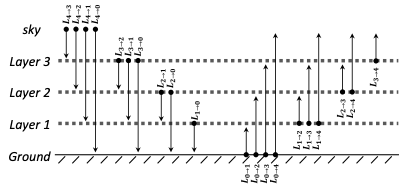
\includegraphics{Figures/辐射过程及辐射通量计算/三层植被长波辐射传输示意图.png}
\caption{三层植被长波辐射传输示意图。4:天空,0:地面,1-3为植被层次,$L_{4 \rightarrow 3}$表示大气到达第三层植被的长波辐射,其他同。}
\label{fig:三层植被长波辐射传输示意图}
\end{figure}
}



从计算示意图来看,仿佛有点复杂,因为需要计算每两层之间的辐射传输量,其实不然。我们把计算式子写出来如下。
从天空下行的长波辐射到达每一层的量为:
\begin{equation}
\begin{aligned} L_{4 \rightarrow 3} &=S_{3} L_{a} \\ L_{4 \rightarrow 2} &=\left(1-S_{3}\right) S_{2} L_{a} 
    \\ L_{4 \rightarrow 1} &=\left(1-S_{2}-S_{3}+S_{2} S_{3}\right) S_{1} L_{a} \\ 
    L_{4 \rightarrow 0} &=\left(1-S_{1}-S_{2}-S_{3}+S_{1} S_{2}+S_{1} S_{3}+S_{2} S_{3}-S_{1} S_{2} S_{3}\right) L_{a} \end{aligned}
\end{equation}
上式中,$S_n$表示第$n$层的阴影(等于太阳辐射传输中入射漫射辐射植被阴影)。为了简化,$L_{atm}\downarrow$简写为$L_a$。从第3层植被向下到达各层的辐射量为:
\begin{equation}
\begin{array}{l}L_{3 \rightarrow 2}=S_{2}\left(L_{3 \downarrow}+L_{3}\right) \\
     L_{3 \rightarrow 1}=\left(1-S_{2}\right) S_{1}\left(L_{3 \downarrow}+L_{3}\right) \\
      L_{3 \rightarrow 0}=\left(1-S_{1}-S_{2}+S_{1} S_{2}\right)\left(L_{3 \downarrow}+L_{3}\right)\end{array}
\end{equation}
上式中$L_3\downarrow$为从第3层植被向下穿透的长波辐射,$L_3$为第3层植被自身发射的长波辐射。
同理,从第2层植被及第1层植被向下到达各层的辐射量分别为:
\begin{equation}
\begin{array}{l}L_{2 \rightarrow 1}=S_{1}\left(L_{2 \downarrow}+L_{2}\right) \\ 
    L_{2 \rightarrow 0}=\left(1-S_{1}\right)\left(L_{2 \downarrow}+L_{2}\right) \\
     L_{1 \rightarrow 0}=L_{1 \downarrow}+L_{1}\end{array}
\end{equation}
将以上的表达式经过简单整理,向下达到每一层的辐射量可以写成矩阵相乘的形式:
\begin{equation}
{L}_{d}=\left(\begin{matrix}0&L_{1\downarrow}+L_1&L_{2\downarrow}+L_2&L_{3\downarrow}+L_3&L_a\\
\end{matrix}\right)\left(\begin{matrix}0&&&&\\a_{10}&0&&&\\a_{20}&a_{21}&0&&
    \\a_{30}&a_{31}&a_{32}&0&\\a_{40}&a_{41}&a_{42}&a_{43}&0\\\end{matrix}\right)
\end{equation}
上式中右边的系数矩阵为:
\begin{equation}
\left(\begin{matrix}0&&&&\\1&0&&&\\1-S_1&S_1&0&&\\1-S_1-S_2+S_1S_2&{\left(1-S_2\right)S}_1&S_2&0&\\
    1-S_1-S_2-S_3+S_1S_2+S_1S_3+S_2S_3-S_1S_2S_3&\left(1-S_2-S_3+S_2S_3\right)S_1&
    \left(1-S_3\right)S_2&S_3&0\\\end{matrix}\right)    
\end{equation}  
上次空白处表示0。若一层有多种PFT,其$L_n$计算为:
\begin{equation}
L_{n}=\sum f_{ci} \varepsilon_{i} \sigma T_{vi}^{4}
\end{equation}
$L_{n\downarrow}$计算为:
\begin{equation}
\begin{aligned} L_{3 \downarrow} &=\sum \frac{S_{3i}\left(1-\varepsilon_{3i}\right)}{S_{3}} L_{4 \rightarrow 3} \\ L_{2 \downarrow} &=\sum \frac{S_{2 i}\left(1-\varepsilon_{2 i}\right)}{S_{2}}\left(L_{4 \rightarrow 2}+L_{3 \rightarrow 2}\right) \\ L_{1 \downarrow} &=\sum \frac{S_{1 i}\left(1-\varepsilon_{1 i}\right)}{S_{1}}\left(L_{4 \rightarrow 1}+L_{3 \rightarrow 1}+L_{2 \rightarrow 1}\right) \end{aligned}
\end{equation}
上式中$S_{ni}$表示第$n$层植被PFT $i$的阴影面积,$\frac{\sum{S_{ni}\left(1-\varepsilon_{ni}\right)}}{S_n}$为每一层的属性,$\varepsilon_{ni}$为单独PFT属性。
先算$L_{3\downarrow}$,然后计算$L_{2\downarrow}$(需要$L_3$的计算结果),接着计算 $L_{1\downarrow}$,容易计算得到
\begin{equation}
L_{v} \downarrow=L_{4 \rightarrow 0}+L_{3 \rightarrow 0}+L_{2 \rightarrow 0}+L_{1 \rightarrow 0} \text {, 即 } \boldsymbol{L}_{\boldsymbol{d}}[0]
\end{equation}
\begin{equation}
L_{g}=\left(1-\varepsilon_{g}\right) L_{v} \downarrow+\varepsilon_{g} \sigma T_{g}^{4}
\end{equation}
从土壤向上发射的辐射$L_g$到达每一层植被的计算类似大气长波的向下传输:
\begin{equation}
\begin{array}{l}L_{0 \rightarrow 1}=S_{1} L_{g} \\ L_{0 \rightarrow 2}=\left(1-S_{1}\right) S_{2} L_{g}
     \\ L_{0 \rightarrow 3}=\left(1-S_{1}-S_{2}+S_{1} S_{2}\right) S_{3} L_{g} \\
      L_{0 \rightarrow 4}=\left(1-S_{1}-S_{2}-S_{3}+S_{1} S_{2}+S_{1} S_{3}+S_{2} S_{3}-S_{1} S_{2} S_{3}\right) L_{g}\end{array}
\end{equation}
从第1层植被向上到达各层的辐射量为:
\begin{equation}
\begin{array}{l}L_{1 \rightarrow 2}=S_{2}\left(L_{1 \uparrow}+L_{1}\right) \\
     L_{1 \rightarrow 3}=\left(1-S_{2}\right) S_{3}\left(L_{1 \uparrow}+L_{1}\right) \\
      L_{1 \rightarrow 4}=\left(1-S_{2}-S_{3}+S_{2} S_{3}\right)\left(L_{1 \uparrow}+L_{1}\right)\end{array}
\end{equation}
上式中$L_1\uparrow$为从第1层植被向上穿透的长波辐射,$L_1$为第1层植被自身发射的长波辐射。同理,从第2层植被及第3层植被向上到达各层的辐射量分别为:
\begin{equation}
\begin{aligned} L_{2 \rightarrow 3} &=S_{3}\left(L_{2 \uparrow}+L_{2}\right) \\
     L_{2 \rightarrow 4} &=\left(1-S_{3}\right)\left(L_{2 \uparrow}+L_{2}\right) \\ 
     L_{3 \rightarrow 4} &=L_{3 \uparrow}+L_{3} \end{aligned}
\end{equation}
将以上的表达式经过简单整理,向上到达每层的辐射量同样可以写成矩阵相乘的形式:
\begin{equation}
{L}_{u}=\left(\begin{matrix}L_g&L_{1\uparrow}+L_1&L_{2\uparrow}+L_2&L_{3\uparrow}+L_3&0\\\end{matrix}
\right)\left(\begin{matrix}0&a_{01}&a_{02}&a_{03}&a_{04}\\&0&a_{12}&a_{13}&a_{14}\\
    &&0&a_{23}&a_{24}\\&&&0&a_{34}\\&&&&0\\\end{matrix}\right)
\end{equation}
上式中右边的系数矩阵为:
\begin{equation}
\left(\begin{matrix}0&S_1&\left(1-S_1\right)S_2&\left(1-S_1-S_2+S_1S_2\right)S_3&
    1-S_1-S_2-S_3+S_1S_2+S_1S_3+S_2S_3-S_1S_2S_3\\&0&S_2&{\left(1-S_2\right)S}_3&1-S_2-S_3+S_2S_3\\
    &&0&S_3&1-S_3\\&&&0&1\\&&&&0\\\end{matrix}\right)   
\end{equation}
同理,
\begin{equation}
L \uparrow=L_{0 \rightarrow 4}+L_{1 \rightarrow 4}+L_{2 \rightarrow 4}+L_{3 \rightarrow 4}, \text { 即 } \boldsymbol{L}_{\boldsymbol{u}}[4]
\end{equation}
到达每一层植被(或地面、天空)的辐射即为
\begin{equation}
L=L_{d}+L_{u}
\end{equation}
单个PFT所吸收的辐射量为
\begin{equation}
\overrightarrow{L_{v l}}=\frac{s_{ni}}{s_{n}} \varepsilon_{ni} L_{* \rightarrow n}-2 f_{ci} \varepsilon_{i} \sigma T_{vi}^{4}
\end{equation}
$L_{\ast\rightarrow n}$即为到达每一层的辐射,即为$L[n]$。注意上式是整个归一化面积上的计算结果,
或者说是在整个土壤$column$上的计算,单位面积上的吸收还需要除以各自的覆盖度$f_{ci}$。


在湍流迭代求解植被温度时,我们还需要用到$\overrightarrow{L_{vl}}$对自身温度的偏导数。PFT吸收的长波辐射来自身发射的部分可计算如下
对于第1层植被:
\begin{equation}
f_{ci} \varepsilon_{vi} \sigma T_{vi}^{4}\left(1-\varepsilon_{g}\right) S_{i} \varepsilon_{vi}
\end{equation}
对于第2层植被:
\begin{equation}
f_{ci} \varepsilon_{vi} \sigma T_{vi}^{4}\left[\left(1-S_{1}\right)+\sum S_{1 i}\left(1-\varepsilon_{1 i}\right)\right]
\left(1-\varepsilon_{g}\right)\left[\left(1-S_{1}\right)+\sum S_{1 i}\left(1-\varepsilon_{1 i}\right)\right] S_{i} \varepsilon_{vi}
\end{equation}
对于第3层植被:
\begin{equation}
\begin{aligned} 
    f_{c i} \varepsilon_{v i} \sigma T_{v i}^{4}\left[\left(1-S_{1}-S_{2}+S_{1} S_{2}\right)+
    \sum S_{2 i}\left(1-\varepsilon_{2 i}\right)\left[\left(1-S_{1}\right)+\sum S_{1 i}\left(1-\varepsilon_{1 i}\right)\right]\right.\\ 
    \left.+\left(1-S_{2}\right) \sum S_{1 i}\left(1-\varepsilon_{1 i}\right)\right]\left(1-\varepsilon_{g}\right)\left[\left(1-S_{1}-S_{2}+S_{1} S_{2}\right)\right.\\ 
    +\sum S_{1 i}\left(1-\varepsilon_{1 i}\right)\left[\left(1-S_{2}\right)+\sum S_{2 i}\left(1-\varepsilon_{2 i}\right)\right] \\ 
    \left.+\left(1-S_{1}\right) 
    \sum S_{2 i}\left(1-\varepsilon_{2 i}\right)\right] S_{i} \varepsilon_{v i} \end{aligned}
\end{equation}
%\begin{equation}
%\begin{aligned} 
%    f_{ci} \varepsilon_{vi} \sigma T_{vi}^{4}
%    \left[\left(1-S_{1}-S_{2}+S_{1}S_{2}\right)+\sum S_{2i}\left(1-\varepsilon_{2i}\right)
%    \left[\left(1-S_{1}\right)+\sum S_{1i}\left(1-\varepsilon_{1i}\right)\right]\\
%    +\left(1-S_{2}\right) \sum S_{1i}\left(1-\varepsilon_{1i}\right)\right]
%     \left(1-\varepsilon_{g}\right)
%     \left[\left(1-S_{1}-S_{2}+S_{1} S_{2}\right)\\
%      &+\sum S_{1i}\left(1-\varepsilon_{1i}\right)\left[\left(1-S_{2}\right)+\sum S_{2i}\left(1-\varepsilon_{2i}\right)\right] \\ 
%      +\left(1-S_{1}\right) \sum S_{2i}\left(1-\varepsilon_{2i}\right)\right] S_{i} \varepsilon_{vi}
 %\end{aligned}
%\end{equation}
同时需要考虑自身发射的的长波辐射$-2f_{ci}\varepsilon_{vi}\sigma T_{vi}^4$。
$\Delta \overrightarrow{L_{vi}}$为以上两者的和对$T_{vi}$求导,同时需要除以$f_{ci}$ (转换成在单位面积上的值)。 
植被温度最后一次迭代的改变所包含的能量分到$L_v\downarrow$增加
$\Sigma4f_{ci}\varepsilon_{vi}\sigma T_{vi}^3\Delta T_{vi}$,$\overrightarrow{L_{g}}$
增加$\varepsilon_g\Sigma4f_{ci}\varepsilon_{vi}\sigma T_{vi}^3\Delta T_{vi}$,$L\uparrow$增加
$\Sigma 4 f_{ci} \varepsilon_{vi} \sigma T_{vi}^{3} \Delta T_{vi}+\left(1-\varepsilon_{g}\right) \Sigma 4 f_{ci} 
\varepsilon_{vi}\left(1-\varepsilon_{vi}\right) \sigma T_{vi}^{3} \Delta T_{vi}$。

%\end{辐射过程及辐射通量计算}

\chapter{地表湍流交换过程}
%\addcontentsline{toc}{chapter}{地表湍流交换过程}

%\begin{地表湍流交换过程}
\section{基本理论}\label{基本理论}
本部分的对应代码为\texttt{groundfluxes.F90}和\texttt{FRICTION\_VELOCITY.F90}。

在近地面层(距离地面几米到几十米高度)中,地面与大气在垂直方向存在显著的湍流输运,且输运通量与风向几乎不随高度变化(亦称常通量性)。计算中引入了尺度因子,则近地面层的动量$\left|\tau\right|$ ($\rm kg/m/s^2$)、热量 $H$ ($\rm W/m^2$)与水汽 $E$ ($\rm kg/m^2/s$)的湍流输运通量可表示为:
\begin{equation}
|\tau|=\rho_{atm} \sqrt{\left(\overline{\left.u^{\prime} w^{\prime}\right)^{2}}+\overline{\left(\overline{v^{\prime} w^{\prime}}\right)^{2}}\right.}=\rho_{atm} u_{*}^{2}
\end{equation}
(分量形式:$\tau_{x}=\rho_{atm} \overline{u^{\prime} w^{\prime}}, \quad \tau_{y}=\rho_{atm} \overline{v^{\prime} w^{\prime}}$)
\begin{equation}
H=C_{p a} \rho_{atm} \overline{\theta^{\prime} w^{\prime}}=-C_{p a} \rho_{atm} \theta_{*} u_{*}
\end{equation}
\begin{equation}
E=\rho_{atm} \overline{q^{\prime} w^{\prime}}=-\rho_{atm} q_{*} u_{*}
\end{equation}
其中$u^\prime$、$v^\prime$、$w^\prime$、$\theta^\prime$、$q^\prime$分别表示纬向速度、经向速度、垂直速度、位温与比湿的湍流脉动,$C_{pa}$表示干空气的比热容(J/kg/K),$\rho_{atm}$表示大气密度($\rm kg/m^3$),$u_\ast$表示摩擦速度(m/s),$\theta_\ast$表示特征位温(K),$q_\ast$表示特征比湿(kg/kg)。$\rho_{atm}$可由公式$\rho_{atm}=\frac{P_{atm}-0.378e_{atm}}{R_{da}T_{atm}}$计算得到,其中$P_{atm}$表示大气压(Pa),$\ T_{atm}$表示大气温度(K),$R_{da}$表示干空气气体常数(J/kg/K),$\ e_{atm}=\frac{q_{atm}P_{atm}}{0.622+0.378q_{atm}}$表示大气水汽分压(Pa),$q_{atm}$表示大气比湿(kg/kg)。
由常通量性可知$u_\ast$、$\theta_\ast$、$q_\ast$均不随高度而变化。


湍流输运通量(动量、感热和水汽)的计算(即$u_\ast$,$\theta_\ast$,$q_\ast$的表达)来自于近地面层Monin-Obukhov相似性理论。基于该理论的量纲分析,无量纲平均风速($\left|u\right|/u_\ast$)、位温($\theta/\theta_\ast$)、比湿($q/q_\ast$)的垂直梯度可共同依赖于参数$\zeta=\frac{z-d}{L}$的函数:

\begin{equation}\label{kz_u}
\frac{k(z-d)}{u_{*}} \frac{\partial|u|}{\partial z}=\phi_{m}(\zeta)
\end{equation}
\begin{equation}\label{kz_theta}
\frac{k(z-d)}{\theta_{*}} \frac{\partial \theta}{\partial z}=\phi_{h}(\zeta)
\end{equation}
\begin{equation}\label{kz_q}
\frac{k(z-d)}{q_{*}} \frac{\partial q}{\partial z}=\phi_{w}(\zeta)
\end{equation}
其中$k$表示von Karman常数,$z$表示常通量层中的高度(m),$d$表示零平面位移(m),$L$表示Monin-Obukhov长度(m):
\begin{equation}
L=-\frac{u_{*}^{3}}{k\left(\frac{g}{\theta_{v, atm}}\right) \overline{\theta_{v}^{\prime} w^{\prime}}}=\frac{u_{*}^{2} \overline{\theta_{v, atm}}}{k g \theta_{v *}}
\end{equation}
其中$\bar{\theta_{v,atm}}=\bar{\theta_{atm}}(1+0.61\bar{q_{atm}})$表示大气虚位温(K),$\theta_{v\ast}$表示特征虚位温(K)
 $\theta_{v\ast}=\theta_\ast\left(1+0.61\bar{q_{atm}}\right)+0.61\bar{\theta_{atm}}q_\ast$。
 大气位温$\theta_{atm}$由其定义的一阶展开近似给出$\theta_{atm}=T_{atm}+0.0098z_{atm}$。$L$可表征边界层的大气层结稳定度:
 在稳定层结下,湍流输运热量$\bar{\theta_v^\prime w^\prime}<0$,$L>0$;在不稳定层结下,
 $\bar{\theta_v^\prime w^\prime}>0$,$L<0$;在中性层结下,$\bar{\theta_v^\prime w^\prime}=0$,$L\rightarrow\infty$。
 $\phi_x$($x$可表示动量$m$,感热$h$和水汽$w$的对应量)是可用于任何下垫面条件的普适相似性函数,
 它将近地面层的湍流输运通量与$\left|u\right|$、$\theta$和$q$的垂直梯度联系起来,构成了对湍流输运通量进行参数化的理论基础。在中性条件下,$\phi_m=\phi_h=\phi_w=1$。

为得到$u_\ast$、$\theta_\ast$、$q_\ast$的表达,将上述关于$\phi_m\left(\zeta\right)$,$\phi_h\left(\zeta\right)$,
$\phi_w(\zeta)$的微分方程(公式\ref{kz_u}-\ref{kz_q})在近地层的两个任意高度$z_1$和$z_2\ (z_2>z_1)$进行积分,得到如下结果:
\begin{equation}
|u|_{2}-|u|_{1}=\frac{u_{*}}{k}\left[\ln \left(\frac{z_{2}-d}{z_{1}-d}\right)-\psi_{m}\left(\frac{z_{2}-d}{L}\right)+\psi_{m}\left(\frac{z_{1}-d}{L}\right)\right]
\end{equation}

\begin{equation}
\theta_{2}-\theta_{1}=\frac{\theta_{*}}{k}\left[\ln \left(\frac{z_{2}-d}{z_{1}-d}\right)-\psi_{h}\left(\frac{z_{2}-d}{L}\right)+\psi_{h}\left(\frac{z_{1}-d}{L}\right)\right]
\end{equation}

\begin{equation}
q_{2}-q_{1}=\frac{q_{*}}{k}\left[\ln \left(\frac{z_{2}-d}{z_{1}-d}\right)-\psi_{w}\left(\frac{z_{2}-d}{L}\right)+\psi_{w}\left(\frac{z_{1}-d}{L}\right)\right]
\end{equation}
其中函数$\psi_x\left(y\right)\ (x=m,\ h,\ w)$定义为
\begin{equation}
\psi_{x}(y)=\int_{\frac{z_{0 x}}{L}}^{y} \frac{1-\phi_{x}(s)}{s} d s
\end{equation}
$z_{0x}\ (x=m,\ h,\ w)$分别表示动量、感热和水汽的粗糙度。这里取$z_1$为地表高度,$z_2$为大气强迫参考(观测)高度,则有如下边界条件:
\begin{equation}
\begin{array}{cl}z_{1}=z_{0 m}+d:|u|_{1}=0 \quad z_{2}=z_{atm, m}: & |u|_{2}=V_{a}=\sqrt{u_{atm}^{2}+v_{atm}^{2}+U_{c}^{2}} \geq 0.1 \\ 
     z_{1}=z_{0 h}+d: \theta_{1}=\theta_{s} & z_{2}=z_{atm, h}: \theta_{2}=\theta_{atm} \\ 
     z_{1}=z_{0 w}+d: q_{1}=q_{s} & z_{2}=z_{atm, w}: q_{2}=q_{atm}\end{array}
\end{equation}
则方程(\ref{kz_u}-\ref{kz_q})由$z_1$到$z_2$的积分结果为:
\begin{equation}\label{Va}
V_{a}=\frac{u_{*}}{k}\left[\ln \left(\frac{z_{atm, m}-d}{z_{0 m}}\right)-\psi_{m}\left(\frac{z_{atm, m}-d}{L}\right)+\psi_{m}\left(\frac{z_{0 m}}{L}\right)\right]
\end{equation}
\begin{equation}\label{theta_atm-theta_s}
\theta_{atm}-\theta_{s}=\frac{\theta_{*}}{k}\left[\ln \left(\frac{z_{atm, h}-d}{z_{0 h}}\right)-\psi_{h}\left(\frac{z_{atm, h}-d}{L}\right)+\psi_{h}\left(\frac{z_{0 h}}{L}\right)\right]
\end{equation}
\begin{equation}\label{q_atm-qs}
q_{atm}-q_{s}=\frac{q_{*}}{k}\left[\ln \left(\frac{z_{atm, w}-d}{z_{0 w}}\right)-\psi_{w}\left(\frac{z_{atm, w}-d}{L}\right)+\psi_{w}\left(\frac{z_{0 w}}{L}\right)\right]
\end{equation}
这里限制$V_a\geq0.1$是为了避免太小的风速使得感热与潜热过小导致数值溢出。对流速度$U_c$表示对流边界层中的大涡对近地层通量的贡献,计算方案为:
\begin{equation}
U_{c}=0 \quad \zeta=\frac{z_{atm, m}-d}{L} \geq 0 \text { 时(即稳定条件下) }
\end{equation}
\begin{equation}
U_{c}=\beta w_{*} \quad \zeta<0 \text { 时 (即不稳定条件下) }
\end{equation}
其中$w_\ast$表示特征垂直速度$w_\ast={(\frac{-gu_\ast\theta_{v\ast}z_i}{\bar{\theta_{v,atm}}})}^{1/3}$,$z_i=1000m$表示对流边界层高度,
参数$\beta=1$。因为$L$是依赖于$u_\ast$、$\theta_\ast$、$q_\ast$的函数,
故方程(\ref{Va})-(\ref{q_atm-qs})可视为如下形式的方程组:
\begin{equation}\label{FGH}
\left\{\begin{array}{l}F\left(u_{*}, L\left(u_{*}, \theta_{*}, q_{*}\right)\right)=0 \\
      G\left(\theta_{*}, L\left(u_{*}, \theta_{*}, q_{*}\right)\right)=0 \\ 
      H\left(q_{*}, L\left(u_{*}, \theta_{*}, q_{*}\right)\right)=0\end{array}\right.
\end{equation}
若给$U_c$与$L$一个初始猜测,结合大气强迫场提供的$u_{atm}$、$v_{atm}$、$\theta_{atm}$、$q_{atm}$及对应的观测高度$z_{atm,x}(x=m,h,w)$,
初始场提供的$\theta_s$、$q_s$,以及对地表参数$d$和$z_{0x}$的估计,$u_\ast$、$\theta_\ast$、$q_\ast$可通过方程组(\ref{FGH})
进行迭代求解,进而求出动量、感热和水汽通量。

根据\citet{zeng1998effect}的结果,相似性函数$\phi_x$可按照如下方式给出:
\begin{equation}
\left\{\begin{array}{lr}\phi_{m}(\zeta)=0.7 k^{\frac{2}{3}}(-\zeta)^{\frac{1}{3}} & \zeta<-1.574 \text { 时 (即非常不稳定条件下) } \\
      \phi_{m}(\zeta)=(1-16 \zeta)^{-\frac{1}{4}} & -1.574 \leq \zeta<0 \text { 时 (即不稳定条件下) } \\
       \phi_{m}(\zeta)=1+5 \zeta & 0 \leq \zeta \leq 1 \text { 时 (即稳定条件下) } \\ 
       \phi_{m}(\zeta)=5+\zeta & \zeta>1 \text { 时 (即非常稳定条件下) }\end{array}\right.
\end{equation}
\begin{equation}
\left\{\begin{array}{lr}\phi_{h}(\zeta)=\phi_{w}(\zeta)=0.9 k^{\frac{4}{3}}(-\zeta)^{-\frac{1}{3}} & \zeta<-0.465 \text { 时 (即非常不稳定条件下) } \\ 
     \phi_{h}(\zeta)=\phi_{w}(\zeta)=(1-16 \zeta)^{-\frac{1}{2}} & -0.465 \leq \zeta<0 \text { 时 (即不稳定条件下) } \\ 
     \phi_{h}(\zeta)=\phi_{w}(\zeta)=1+5 \zeta & 0 \leq \zeta \leq 1 \text { 时 (即稳定条件下) } \\
      \phi_{h}(\zeta)=\phi_{w}(\zeta)=5+\zeta & \zeta>1 \text { 时 (即非常稳定条件下) }\end{array}\right.
\end{equation}
将$\phi_m$代入风速廓线方程(\ref{Va}),即可得到具体形式:
非常不稳定条件下($\zeta_a=\frac{z_{atm,m}-d}{L}<-1.574$)
\begin{equation}
V_{a}=\frac{u_{*}}{k}\left\{\ln \frac{-1.574 L}{z_{0 m}}-\psi_{m}(-1.574)+
1.14\left[\left(-\zeta_{a}\right)^{\frac{1}{3}}-(1.574)^{\frac{1}{3}}\right]+\psi_{m}\left(\frac{z_{0 m}}{L}\right)\right\}
\end{equation}
不稳定条件下($-1.574\le\zeta_a<0$)
\begin{equation}
V_{a}=\frac{u_{*}}{k}\left\{\ln \frac{z_{atm, m}-d}{z_{0 m}}-\psi_{m}\left(\zeta_{a}\right)+\psi_{m}\left(\frac{z_{0 m}}{L}\right)\right\}
\end{equation}
稳定条件下($0\le\zeta_a\le1$)
\begin{equation}
V_{a}=\frac{u_{*}}{k}\left\{\ln \frac{z_{atm, m}-d}{z_{0 m}}+5 \zeta_{a}-5 \frac{z_{0 m}}{L}\right\}
\end{equation}
非常稳定条件下($\zeta_a>1$)
\begin{equation}
V_{a}=\frac{u_{*}}{k}\left\{\left[\ln \frac{L}{z_{0 m}}+5\right]+\left[5 \ln \zeta_{a}+\zeta_{a}-1\right]-5 \frac{z_{0 m}}{L}\right\}
\end{equation}
其中$\psi_m\left(\zeta\right)=2\ln{(\frac{1+x}{2})}+\ln{\left(\frac{1+x^2}{2}\right)-2}\tan^{-1}{x}+\frac{\pi}{2},x={(1-16\zeta)}^{1/4}$。
将$\phi_h$,$\phi_w$代入温度廓线方程(\ref{theta_atm-theta_s})和水汽廓线方程(\ref{q_atm-qs}),即可得到具体形式:
非常不稳定条件下($\zeta_a=\frac{z_{atm,h}-d}{L}$ 或$ \ \frac{z_{atm,w}-d}{L}\ <-0.465$)
\begin{equation}
\begin{array}{l}\theta_{atm}-\theta_{s}= \\ 
     \frac{\theta_{*}}{k}\left\{\ln \frac{-0.465 L}{z_{0 h}}-\psi_{h}(-0.465)+0.8\left[(0.465)^{-\frac{1}{3}}-\left(-\zeta_{a}\right)^{-\frac{1}{3}}\right]
     +\psi_{h}\left(\frac{z_{0 h}}{L}\right)\right\}\end{array}
\end{equation}
\begin{equation}
\begin{array}{l}q_{atm}-q_{s}= \\ 
     \quad \frac{q_{*}}{k}\left\{\ln \frac{-0.465 L}{z_{0 w}}-\psi_{w}(-0.465)+0.8\left[(0.465)^{-\frac{1}{3}}-
     \left(-\zeta_{a}\right)^{-\frac{1}{3}}\right]+\psi_{w}\left(\frac{z_{0 w}}{L}\right)\right\}\end{array}
\end{equation}
不稳定条件下($-0.465\le\zeta_a<0$)
\begin{equation}
\theta_{atm}-\theta_{s}=\frac{\theta_{*}}{k}\left\{\ln \frac{z_{atm, h}-d}{z_{0 h}}-\psi_{h}
\left(\zeta_{a}\right)+\psi_{h}\left(\frac{z_{0 h}}{L}\right)\right\}
\end{equation}
\begin{equation}
q_{atm}-q_{s}=\frac{q_{*}}{k}\left\{\ln \frac{z_{atm, w}-d}{z_{0 w}}-
\psi_{w}\left(\zeta_{a}\right)+\psi_{w}\left(\frac{z_{0 w}}{L}\right)\right\}
\end{equation}
非常稳定条件下($\zeta_a>1$)
\begin{equation}
\theta_{atm}-\theta_{s}=\frac{\theta_{*}}{k}\left\{\left[\ln \frac{L}{z_{0 h}}+5\right]
+\left[5 \ln \zeta_{a}+\zeta_{a}-1\right]-5 \frac{z_{0 h}}{L}\right\}
\end{equation}
\begin{equation}
q_{atm}-q_{s}=\frac{q_{*}}{k}\left\{\left[\ln \frac{L}{z_{0 w}}+5\right]
+\left[5 \ln \zeta_{a}+\zeta_{a}-1\right]-5 \frac{z_{0 w}}{L}\right\}
\end{equation}
其中$\psi_h\left(\zeta\right)=\psi_w\left(\zeta\right)=2\ln{\left(\frac{1+x^2}{2}\right)}$,$x={(1-16\zeta)}^{1/4}$。
事实上,$L$的初始猜测可由体积理查德森数$R_{ib}$与$\zeta$的关系得到\citep{arya2001introduction}。$R_{ib}$表达为
\begin{equation}
R_{i b}=\frac{\theta_{v, atm}-\theta_{v, s}}{\theta_{v, atm}} \frac{g\left(z_{atm, m}-d\right)}{v_{a}^{2}}
\end{equation}
$R_{ib}$与$\zeta$的关系为$R_{ib}=\zeta[\ln{\left(\frac{z_{atm,h}-d}{z_{0h}}\right)-\psi_h(\zeta)}][lnzatm,m-dz0m-ψm(ζ)]-2$。
$\psi_m(\zeta)$与$\psi_h(\zeta)$由不稳定条件下$\phi_h\left(\zeta\right)=\phi_m^2\left(\zeta\right)=\left(1-16\zeta\right)^{-\frac{1}{2}}$ 
与稳定条件下$\phi_h\left(\zeta\right)=\phi_m\left(\zeta\right)=1+5\zeta$确定。将$\zeta$表达为$R_{ib}$的函数,即得到
\begin{equation}
\left\{\begin{array}{c}\zeta=\frac{R_{i b} \ln \left(\frac{z_{atm, m}-d}{z_{0 m}}\right)}{1-5 \min \left(R_{i b}, 0.19\right)} \ \ \ \ \ \ \  10^{-6} \leq \zeta \leq 2 R_{i b} \geq 0 \text{(即中性或稳定条件下)}
    \\ \zeta=R_{i b} \ln \left(\frac{z_{atm, m}-d}{z_{0 m}}\right) \ \ \ \ \ \ \ \ -100 \leq \zeta \leq-10^{-6} R_{i b}<0 \text{(即中性或稳定条件下)}\end{array}\right.
\end{equation}
通过$R_{ib}$计算得到$\zeta$即可求得$L=\frac{z_{atm,m}-d}{\zeta}$。
以上给出了$u_\ast$、$\theta_\ast$、$q_\ast$的求解过程,于是大气强迫参考高度与地表的动量、感热和水汽通量即可通过其定义求得。
事实上,根据$u_\ast$、$\theta_\ast$、$q_\ast$的表达形式,动量通量$\tau$、感热通量$H$和水汽通量$E$可写为如下阻抗形式:
\begin{equation}
\tau_{x}=-\frac{u_{atm}}{V_{a}} \rho_{atm} u_{*}^{2}=-\rho_{atm} \frac{u_{atm}}{r_{a m}}
\end{equation}
\begin{equation}
\tau_{y}=-\frac{v_{atm}}{v_{a}} \rho_{atm} u_{*}^{2}=-\rho_{atm} \frac{v_{atm}}{r_{a m}}
\end{equation}
\begin{equation}
H=-C_{p a} \rho_{atm} \theta_{*} u_{*}=-\rho_{atm} C_{p a} \frac{\left(\theta_{atm}-\theta_{s}\right)}{r_{a h}}
\end{equation}
\begin{equation}
E=-\rho_{atm} q_{*} u_{*}=-\rho_{atm} \frac{\left(q_{atm}-q_{s}\right)}{r_{a w}}
\end{equation}
其中,空气动力学阻抗系数$r_{am}$、$r_{ah}$、$r_{aw}$(s/m)表达为
\begin{equation}
r_{a m}=\frac{1}{k^{2} V_{a}}\left[\ln \left(\frac{z_{atm, m}-d}{z_{0 m}}\right)-\psi_{m}\left(\frac{z_{atm, m}-d}{L}\right)+\psi_{m}\left(\frac{z_{0 m}}{L}\right)\right]^{2}
\end{equation}
\begin{equation}
\begin{array}{c}r_{a h}=\frac{1}{k^{2} V_{a}}\left[\ln \left(\frac{z_{atm, m}-d}{z_{0 m}}\right)-\psi_{m}\left(\frac{z_{atm, m}-d}{L}\right)+\psi_{m}\left(\frac{z_{0 m}}{L}\right)\right] \\ {\left[\ln \left(\frac{z_{atm, h}-d}{z_{0 h}}\right)-\psi_{h}\left(\frac{z_{atm, h}-d}{L}\right)+\psi_{h}\left(\frac{z_{0 h}}{L}\right)\right]}\end{array}
\end{equation}
\begin{equation}
\begin{array}{c}r_{a w}=\frac{1}{k^{2} V_{a}}\left[\ln \left(\frac{z_{atm, m}-d}{z_{0 m}}\right)-\psi_{m}\left(\frac{z_{atm, m}-d}{L}\right)+\psi_{m}\left(\frac{z_{0 m}}{L}\right)\right] \\ {\left[\ln \left(\frac{z_{atm, w}-d}{z_{0 w}}\right)-\psi_{w}\left(\frac{z_{atm, w}-d}{L}\right)+\psi_{w}\left(\frac{z_{0 w}}{L}\right)\right]}\end{array}
\end{equation}
因此湍流通量可认为由此阻抗模型计算而来。
为方便与地表观测资料进行比较,下面给出地表高度$z_{0x}+d$以上2m的温度比湿和10m的风速计算公式(即对原始微分方程从$z_{0x}+d$到$z_{0x}+d+2$ ($z_{0x}+d+10$) 进行积分)如下:
\begin{equation}
T_{2 m}=\theta_{s}+\frac{\theta_{*}}{k}\left[\ln \left(\frac{2+z_{0 h}}{z_{0 h}}\right)-\psi_{h}\left(\frac{2+z_{0 h}}{L}\right)+\psi_{h}\left(\frac{z_{0 h}}{L}\right)\right]
\end{equation}
\begin{equation}
q_{2 m}=q_{s}+\frac{q_{*}}{k}\left[\ln \left(\frac{2+z_{0 w}}{z_{0 w}}\right)-\psi_{w}\left(\frac{2+z_{0 w}}{L}\right)+\psi_{w}\left(\frac{z_{0 w}}{L}\right)\right]
\end{equation}
\begin{equation}
u_{10 m}=\frac{u_{*}}{k}\left[\ln \left(\frac{10+z_{0 m}}{z_{0 m}}\right)-\psi_{m}\left(\frac{10+z_{0 m}}{L}\right)+\psi_{m}\left(\frac{z_{0 m}}{L}\right)\right]
\end{equation}


\section{无植被覆盖地表湍流通量的计算方案}\label{无植被覆盖地表湍流通量的计算方案}
当陆地表面没有植被覆盖(即裸土、冰川、水体等表面)或植被已被积雪掩埋时,湍流通量按照无植被覆盖情形的方案计算(表\ref{tab:物理常数} )。
对于任一地表类型斑块,植被所占比例为$f_{veg}$(当前取值为0或1),植被粗糙度为$z_{vm}$
(表\ref{tab:USGS地表粗糙度和零平面位移}给出了按照USGS分类下的24种土地覆盖类型的对应参数值),则被积雪掩埋的植被占总植被的比例为
\begin{equation}
wt=\frac{0.1 z_{{sno}}}{z_{v m}+0.1 z_{{sno}}}
\end{equation}
其中$z_{sno}$表示积雪厚度(m)。于是斑块中的有效植被比例$f_{sig}=\left(1-wt\right)f_{veg}$,
无植被覆盖比例为$\left(1-f_{sig}\right)$。

\begin{table}[]
\centering
\caption{物理常数}
\label{tab:物理常数}
\begin{tabular}{lccc}
\toprule
变量名&缩写&数值&单位 \\\midrule
干空气气体常数            & $R_{da}$                       & 287.04     & J/kg/K  \\ 
水汽气体常数             & $R_{wv}$                       & 461.296     & J/kg/K  \\
干空气比热容             & $C_{pa} $                      & 1004.64    & J/kg/K  \\
液态水比热容             & $C_{pl}$                       & 4188.0     & J/kg/K  \\
固态水比热容             & $C_{pi}$                       & 2117.27    & J/kg/K  \\
von Karman常数       & $k$                               & 0.4        &    -     \\
重力加速度              & $g$                               & 9.80616    & $\rm m/s^2$    \\
Stefan-Boltzmann常数 & $\sigma$           & $5.67\times\rm 10^{-8}$  & $\rm W/m^2/K^4$ \\
液态水凝结温度            & $T_f$                            & 273.16     & K       \\
液态水密度              & $\rho_{liq}$    & 1000       & $\rm Kg/m^3$   \\
固态水密度              & $\rho_{ice}$    & 917        & $\rm Kg/m^3$   \\
液态水蒸发潜热            & $\lambda_v$       & $2.5104\times\rm 10^{6}$ & J/kg    \\
固态水升华潜热            & $\lambda_s$       & $2.8440\times\rm 10^{6}$ & J/kg    \\
固态水液化潜热            & $L_f$                           & $0.3336\times10^6$ & J/kg    \\
液态水热力传导率           & $\lambda_{liq}$ & 0.57       & W/m/K   \\
固态水热力传导率           & $\lambda_{ice}$ & 2.29       & W/m/K   \\
空气热力传导率            & $\lambda_a$       & 0.023      & W/m/K      \\\bottomrule
\end{tabular}
\end{table}



% Please add the following required packages to your document preamble:
% \usepackage{booktabs}
\begin{table}[]
\centering
\caption{基于USGS分类的24种土地覆盖类型的地表粗糙度和零平面位移}
\label{tab:USGS地表粗糙度和零平面位移}
\begin{tabular}{@{}lcc@{}}
\toprule
土地覆盖类型    & 植被粗糙度($z_{0x}$) & 零平面位移($d$) \\ \midrule
城市        & 0.1              & 0.667    \\
干旱农田与牧场   & 0.1              & 0.667    \\
灌溉农田与牧场   & 0.1              & 0.667    \\
干湿混合农田与牧场 & 0.1              & 0.667    \\
农田草地过渡带   & 0.1              & 0.667    \\
农田林地过渡带   & 0.1              & 0.667    \\
草地        & 0.1              & 0.667    \\
灌木地       & 0.05             & 0.333    \\
草地灌木地混合带  & 0.05             & 0.333    \\
稀树草原      & 0.1              & 0.667    \\
落叶阔叶林     & 2.0              & 13.333   \\
落叶针叶林     & 1.7              & 11.333   \\
常绿阔叶林     & 3.5              & 23.333   \\
常绿针叶林     & 1.7              & 11.333   \\
混合森林      & 2.0              & 13.333   \\
内陆水体      & 0.1              & 0.667    \\
草本湿地      & 0.1              & 0.667    \\
森林湿地      & 3.5              & 23.333   \\
贫瘠稀疏植被    & 0.05             & 0.333    \\
草本苔原      & 0.1              & 0.667    \\
森林苔原      & 0.1              & 0.667    \\
混合苔原      & 0.1              & 0.667    \\
裸土苔原      & 0.1              & 0.667    \\
雪盖或冰川     & 0.1              & 0.667    \\ \bottomrule
\end{tabular}
\end{table}

陆地表面可分为被积雪覆盖与未被积雪覆盖两部分。根据\citet{swenson2012new}提供的方法,
被积雪覆盖的地表面积比例$f_{sno}$可分为两步计算:在积分开始时若有降雪发生,则新一步的$f_{sno}$更新为
\begin{equation}
f_{{sno }}^{(n+1)}=1-\left(1-\tanh \left(0.1 p_{i} \Delta t\right)\right)\left(1-f_{{sno }}^{(n)}\right) \leq 1.0
\end{equation}
其中$p_i$为降雪率($\rm kg/m^2/s$),$\Delta t$为积分步长(s);在水热过程模拟结束后,若有积雪融化发生,则$f_{sno}$更新为
\begin{equation}
f_{sno}^{(n+1)}=\tanh \frac{100 z_{s n o}^{2}}{2.5 z_{0 m, s o i} W_{sno}}
\end{equation}
其中$W_{sno}$为雪水当量(mm),$z_{0m,soi}$为未被积雪覆盖时的地表粗糙度。
对于无植被覆盖部分的陆地表面,湍流输运通量只存在于地表与大气之间。此时动量通量$\tau_b$、感热通量$H_b$和水汽通量$E_b$表达为:
\begin{equation}
\tau_{b, x}=-\left(1-f_{sig}\right)\left(\rho_{atm} \frac{u_{atm}}{r_{a m}}\right)
\end{equation}
\begin{equation}
\tau_{b, y}=-\left(1-f_{sig}\right)\left(\rho_{atm} \frac{v_{atm}}{r_{a m}}\right)
\end{equation}
\begin{equation}
H_{b}=-\left(1-f_{sig}\right) \rho_{atm} C_{p a} \frac{\left(\theta_{atm}-T_{g}\right)}{r_{a h}}
\end{equation}
\begin{equation}
E_{b}=-\left(1-f_{sig}\right) \rho_{atm} \frac{\left(q_{atm}-q_{g}\right)}{r_{a w}}
\end{equation}
其中$T_g$表示地表温度(K)(当有积雪覆盖(即$f_{sno}>0$)时,$T_g$为最上层积雪的温度$T_{snl+1}$;
无积雪覆盖时,$T_g$为第一层土壤的温度$T_1$),$q_g$表示地表空气比湿(kg/kg),其计算公式为:
\begin{equation}
q_{g}=\left(1-f_{{sno }}\right) q_{{soil }}+f_{{sno }} q_{{sno }}
\end{equation}
其中积雪表面的比湿$q_{sno}$为温度在$T_{snl+1}$时的饱和比湿$q_{sno}=q_{sat}^{T_{snl+1}}$
(计算方案见章节 \ref{饱和水汽压(比湿)及其随温度的变化}),土壤表面的比湿$q_{soil}$视为正比于温度在$T_1$时的饱和比湿$q_{sat}^{T_1}:q_{soil}=\alpha_{soil}q_{sat}^{T_1}$,
比例系数$\alpha_{soil}$为表层土壤水势$\psi_1$(mm)的函数\citep{philip1957theory}:$\alpha_{soil}=exp\left(\frac{\psi_1g}{{10}^3R_{wv}T_1}\right)$,
其中$R_{wv}$表示水汽气体常数(J/kg/K)。表层土壤水势$\psi_1$的计算公式为$\psi_1=\psi_{sat,1}s_1^{-B_1}\geq-1\ast{10}^8$,
$\psi_{sat,1}$表示表层饱和土壤水势(mm),$B_1$表示表层土壤\citet{clapp1978empirical}参数(均由地表参数数据集提供)。$s_1$表示表层土壤对于饱和状态时的相对湿度:
\begin{equation}
\begin{array}{c}s_{1}=0.001 \quad \text { if } \theta_{{sat }, 1}<1 * 10^{-6} \\ s_{1}=\frac{1}{\Delta z_{1} \theta_{{sat }, 1}}\left[\frac{w_{l i q, 1}}{\rho_{l i q}}+\frac{w_{i c e, 1}}{\rho_{{ice }}}\right] \quad 0.001 \leq s_{1} \leq 1.0 \text { if } \theta_{\text {sat }, 1} \geq 1 * 10^{-6}\end{array}
\end{equation}
其中$∆z1$为表层土壤厚度(m),$\rho_{liq}$和$\rho_{ice}$分别为液态水和固态水密度($\rm kg/m^3$),
$w_{liq,1}$和$w_{ice,1}$分别为表层土壤液态水和固态水含量($\rm kg/m^2$),
$\theta_{sat,1}$表示表层土壤体积含水量(即孔隙度,$\rm mm^3/mm^3$)。
注:为避免土壤水含量极低时轻微的土壤水变化会导致$q_{soil}$变化过大,
当$q_{sat}^{T_1}>q_{atm}$且$q_{atm}>q_{soil}$时,取$q_{soil}=q_{atm}$且$\frac{dq_{soil}}{dT_1}=0$。


由于地表无植被覆盖,在计算阻抗系数$r_{am}$、$r_{ah}$、$r_{aw}$时,零平面位移取为$d=0$。
动量粗糙度在有积雪覆盖(即$f_{sno}>0$)时取为$z_{0m}=0.0024$,无积雪覆盖时取为$z_{0m}=0.01$。
由于动量输运会受到湍流波中气压波动的影响,而热量与水汽输运只受到分子扩散的影响,
故感热与水汽粗糙度不同于动量粗糙度如下\citep{zeng1998effect}:
\begin{equation}
z_{0 h}=z_{0 w}=z_{0 m} \exp \left(-0.13\left(u_{*} \cdot z_{0 m} / v\right)^{0.45}\right)
\end{equation}
其中$\upsilon=1.5\times{10}^{-5}$($\rm m^2/s$)表示空气的动力粘性系数。


结合以上计算方案,无植被覆盖部分的地表湍流输运通量可按如下流程计算:
\begin{enumerate}
     \item 给出$U_c$的初始猜测如下:
     \begin{equation}
          \begin{array}{cc}U_{c}=0 & \theta_{v, atm}-\theta_{v, s} \geq 0(\text { 即稳定条件下 }) \\ U_{c}=0.5 & \theta_{v, atm}-\theta_{v, s}<0(\text { 即不稳定条件下 })\end{array}
          \end{equation}
     \item 通过$R_{ib}$给出$L$的初始猜测;
     \item 以下过程迭代6次,以求得$u_\ast$,$\theta_\ast$,$q_\ast$:\\
     a. 通过风速、温度、比湿的微分方程积分结果求得$u_\ast$,$\theta_\ast$,$q_\ast$ \\
     b. 更新感热与水汽粗糙度$z_{0h}$,$z_{0w}$ \\
     c. 计算特征虚位温$\theta_{v\ast}$ \\
     d. 更新大气风速$V_a\left(U_c\right)$ \\
     e. 计算新一步L,并计算$\zeta$,根据稳定性条件限制$\zeta$的取值范围 \\
     f. 根据限制条件后的$\zeta$重新计算$L=\frac{z_{atm,m}}{\zeta}$ \\
     每次迭代完成后,判断L是否改变符号,若改变符号超过4次,则视为中性条件,跳出迭代过程,以避免在稳定与不稳定条件之间来回变化;
     \item 计算空气动力学阻抗系数$r_{am}$,$r_{ah}$,$r_{aw}$
     \item 计算动量通量$\tau_b$、感热通量$H_b$和水汽通量$E_b$
     \item 计算2m温度与比湿$T_{2m}$,$q_{2m}$
     \item 在计算地表温度并基于该温度对感热与水汽通量进行更新时,需给出感热与水汽通量针对地表温度的变化率:
     \begin{equation}
          \frac{\partial H_{b}}{\partial T_{g}}=\left(1-f_{sig}\right) \frac{\rho_{atm} C_{p a}}{r_{a h}}
          \end{equation}
          \begin{equation}
          \frac{\partial E_{b}}{\partial T_{g}}=\left(1-f_{sig}\right) \frac{\rho_{atm}}{r_{a w}} \frac{d q_{g}}{d T_{g}}
     \end{equation}
     其中$\frac{dq_g}{dT_g}=\left[\left(1-f_{sno}\right)\alpha_{soil}+f_{sno}\right]\frac{q_{sat}^{T_g}}{dT_g}$,$\frac{q_{sat}^{T_g}}{dT_g}$的计算见章节 \ref{饱和水汽压(比湿)及其随温度的变化}。
     阻抗系数$r_{ah}$、$r_{aw}$对于温度的变化率无法解析给出,故暂时忽略。

 \end{enumerate}


\section{一维植被湍流交换模型}\label{一维植被湍流交换模型}
对于有植被覆盖部分的陆地表面,陆地与大气总湍流输运通量为植被冠层顶空气与大气之间的湍流输送,其动量通量$\tau_p$、感热通量$H_p$和水汽通量$E_p$表达为:
\begin{equation}
\tau_{p, x}=-f_{\text {sig }} \rho_{atm} \frac{u_{atm}}{r_{a m}}
\end{equation}
\begin{equation}
\tau_{p, y}=-f_{sig} \rho_{atm} \frac{v_{atm}}{r_{a m}}
\end{equation}
\begin{equation}
H_{p}=-f_{sig} \rho_{atm} C_{p a} \frac{\left(\theta_{atm}-T_{s}\right)}{r_{a h}}
\end{equation}
\begin{equation}
E_{p}=-f_{\text {sig }} \rho_{atm} \frac{\left(q_{atm}-q_{s}\right)}{r_{a w}}
\end{equation}
由于此时湍流通量与叶片温度相互耦合,故阻抗系数$r_{am}$、$r_{ah}$、$r_{aw}$与植被冠层顶空气温度和比湿$T_s$、$q_s$将随叶片温度一起采用牛顿迭代法进行求解(见章节 \ref{植被叶片温度计算})。
本节就感热与水汽通量先给出其求解的理论表达。


假设植被冠层空气的比热容为0,则它与大气之间的热量与水汽交换可被两部分通量抵消平衡:
一是地表与植被冠层顶空气之间的湍流通量,二是植被表面(茎、叶等)与植被冠层顶空气之间的湍流通量。
对于植被的描述,植被生理过程采用\citet{dai2004two}提出的双大叶模型,即将叶片分为阴叶(无阳光照射)与阳叶(有阳光照射)两部分。
阳叶的比例表达为:
\begin{equation}
f_{sun}=\frac{1-\exp p(-K \cdot LAI)}{K \cdot LAI}
\end{equation}
其中$LAI$为叶面积指数,$K$为太阳辐射消光系数(见章节 \ref{短波吸收辐射通量}),${10}^{-6}\le K \cdot LAI\le40$。
当白天植被吸收的太阳辐射小于1 W/m$^2$ 或白天结束时,$f_{sun}=0$。叶面积指数也对应表达为两部分:
\begin{equation}
\begin{array}{c}LAI_{sun}=LAI \cdot f_{sun} \\ LAI_{sha}=LAI \cdot \left(1-f_{sun}\right)\end{array}
\end{equation}
植被能量平衡过程,即植被的湍流通量与叶片温度仍采用单叶模型计算。主要过程描述如下:


当地表有植被覆盖时,假设植被树冠水平空间分布均匀且为单层结构(即一维植被结构),则植被冠层顶空气与大气之间的感热通量$H_p$可与下列三项平衡:
\begin{equation}
H_{p}=H_{p g}+H_{p v}
\end{equation}
其中$H_{pg}$表示地表与植被冠层空气顶之间的感热,$H_{pv,sun}$表示叶片表面与植被冠层空气顶之间的感热:
\begin{equation}
H_{p g}=-f_{sig} \rho_{atm} C_{pa} \frac{\left(T_{s}-T_{g}\right)}{r_{a h}^{\prime}}
\end{equation}
\begin{equation}
H_{p v}=-f_{sig} \rho_{atm} C_{pa}(LAI+S A I) \frac{\left(T_{s}-T_{v}\right)}{r_{b}}
\end{equation}
其中$T_v$表示叶片温度(K),$T_s$表示定义在高度$z_{0h}+d$上的植被冠层顶空气温度(K),$SAI$表示茎面积指数,$r_b$表示叶面边界层阻抗(s/m),
$r_{ah}^\prime$表示地表与植被冠层顶空气之间的感热阻抗(s/m)。示意图如下(图 \ref{fig:有植被覆盖部分的陆地表面感热通量示意图}):
{
\begin{figure}[]
\centering
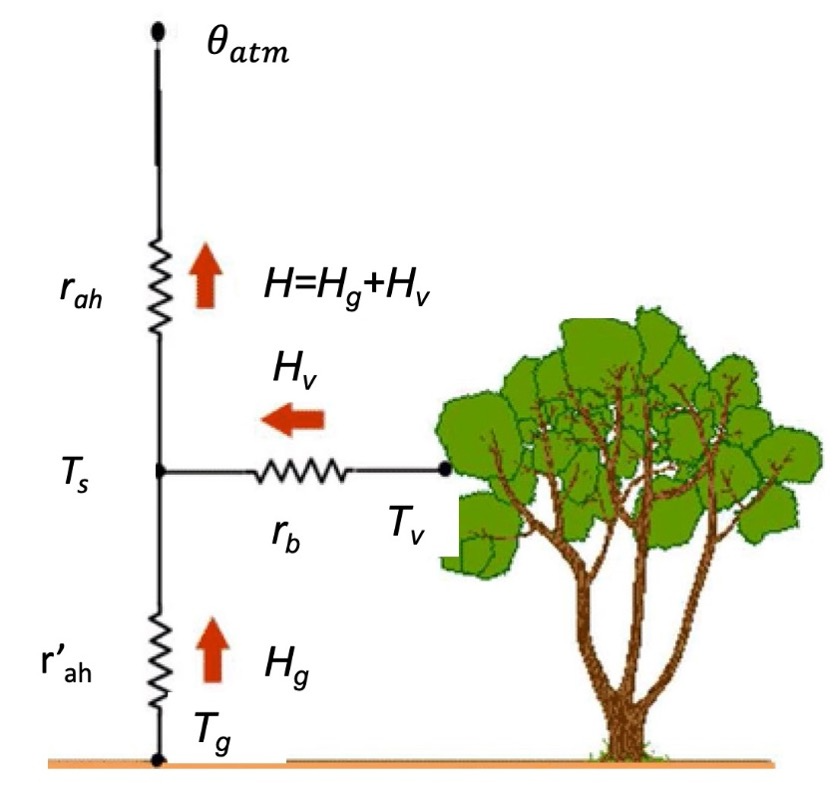
\includegraphics{Figures/地表湍流交换过程/有植被覆盖部分的陆地表面感热通量示意图.png}
\caption{有植被覆盖部分的陆地表面感热通量示意图。}
\label{fig:有植被覆盖部分的陆地表面感热通量示意图}
\end{figure}
}
将$H_p$、$H_{pg}$、$H_{pv}$的表达式代入平衡方程,即可解出$T_s$如下:
\begin{equation}
T_{s}=\frac{c_{a}^{h} \theta_{atm}+c_{g}^{h} T_{g}+c_{v}^{h} T_{v}}{c_{a}^{h}+c_{g}^{h}+c_{v}^{h}}
\end{equation}
其中$c_a^h=\frac{1}{r_{ah}}$,$c_g^h=\frac{1}{r_{ah}^\prime}$,$c_v^h=\frac{LAI+SAI}{r_b}$,
将$T_s$的表达式代回,即可将$H_p$、$H_{pg}$、$H_{pv}$全部写为$\theta_{atm}$、$T_g$、$T_v$的函数,例如:
\begin{equation}
H_{p v}=-f_{sig} \rho_{atm} C_{p a}\left[c_{a}^{h} \theta_{atm}+c_{g}^{h} 
T_{g}+c_{v}^{h} T_{v}-\left(c_{a}^{h}+c_{g}^{h}+c_{v}^{h}\right)
T_{v}\right] \frac{c_{v}^{h}}{c_{a}^{h}+c_{g}^{h}+c_{v}^{h}}
\end{equation}


同样地,植被冠层顶空气与大气之间的水汽通量$E_p$可与下列三项平衡:
\begin{equation}
E_{p}=E_{p g}+E_{p v}
\end{equation}
其中$E_{pg}$表示地表与植被冠层顶空气之间的水汽通量,$E_{pv}$表示叶片表面与植被冠层顶空气之间的水汽通量:
\begin{equation}
E_{pg}=-f_{sig} \rho_{atm} \frac{\left(q_{s}-q_{g}\right)}{r_{a w}^{\prime}}
\end{equation}

\begin{equation}
E_{pv}=-f_{sig} \rho_{atm} \frac{\left(q_{s}-q_{s a t}^{T v}\right)}{r_{t o t a l}}
\end{equation}
其中$q_{sat}^{T_v}$表示叶片温度在$T_v$下的饱和比湿(kg/kg),$q_s$表示定义在高度$z_{0w}+d$上的植被冠层顶空气比湿(kg/kg),
$q_g$表示地表空气比湿(kg/kg,其表达见章节 \ref{无植被覆盖地表湍流通量的计算方案}),$r_{aw}^\prime$表示地表与植被冠层顶空气之间的水汽交换阻抗(s/m)。
$r_{total}$表示植被表面与植被冠层顶空气之间水汽交换的总阻抗(s/m),
它来自叶面边界层阻抗$r_b$和气孔阻抗$r_{s,sun}\left(r_{s,sha}\right)$的双重贡献。
植被表面与植被冠层空气之间的水汽交换包含两部分:湿的叶面与茎面的蒸发水汽与干叶表面的蒸腾水汽。
湿的叶面茎面积占总叶面茎面积的比例 \citep{dickinson1993biosphere} 为:
\begin{equation}
f_{w e t}=\left(\frac{W_{c a n}}{W_{c a n, \max }}\right)^{2 / 3} \leq 1.0
\end{equation}
其中$W_{can}$表示植被表面储水量($\rm kg/m^2$,其计算见章节 \ref{植被冠层截留}),$W_{can,max}$表示植被表面最大储水量
($\rm kg/m^2$),$W_{can,max}=0.1f_{sig}\left(LAI+SAI\right)$。
有植被覆盖部分的陆地表面水热通量示意图见图\ref{fig:有植被覆盖部分的陆地表面水汽通量示意图}:
{
\begin{figure}[]
\centering
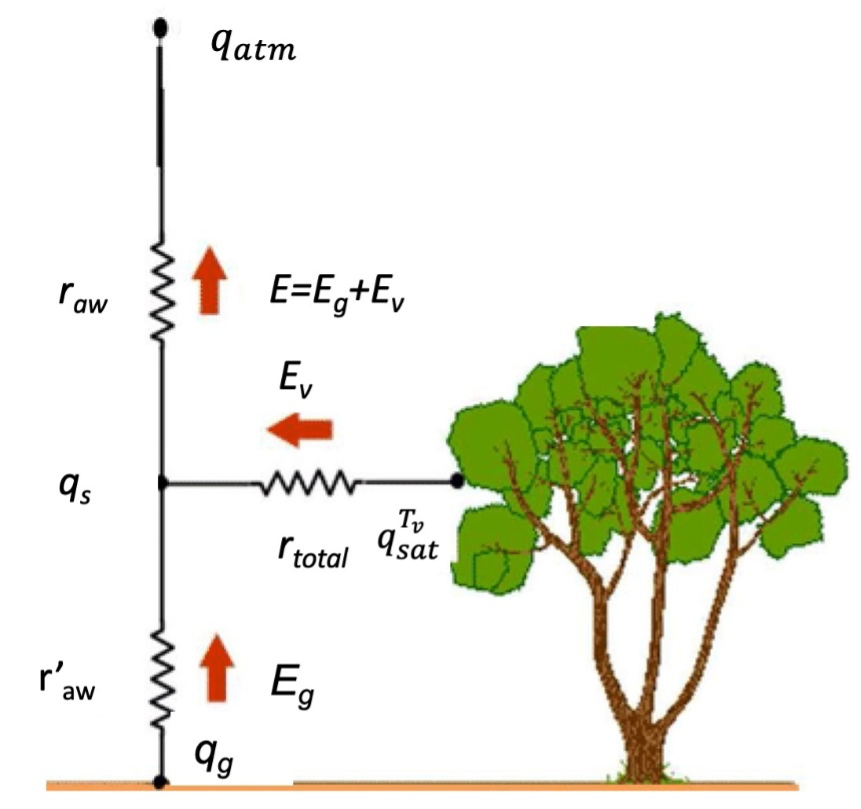
\includegraphics{Figures/地表湍流交换过程/有植被覆盖部分的陆地表面水汽通量示意图.png}
\caption{有植被覆盖部分的陆地表面水汽通量示意图。}
\label{fig:有植被覆盖部分的陆地表面水汽通量示意图}
\end{figure}
}
将$E_p$、$E_{pg}$、$E_{pv}$的表达式代入平衡方程,即可解出$q_s$如下:
\begin{equation}
q_{s}=\frac{c_{a}^{w} q_{atm}+c_{g}^{w} q_{g}+c_{v}^{w} q_{s a t}^{T_{v}}}{c_{a}^{w}+c_{g}^{w}+c_{v}^{w}}
\end{equation}
其中$c_a^w=\frac{1}{r_{aw}}$,$c_g^w=\frac{1}{r_{aw}^\prime}$,$c_v^w=\frac{1}{r_{total}}$,
将$q_s$的表达式代回,即可将$E_p$、$E_{pg}$、$E_{pv}$全部写为$q_{atm}$、$q_g$、$q_{sat}^{T_v}$的函数,例如:
\begin{equation}
E_{p v}=-f_{sig} \rho_{atm}\left[c_{a}^{w} q_{atm}+c_{g}^{w} q_{g}+c_{v}^{w} q_{s a t}^{T_{v}}-
\left(c_{a}^{w}+c_{g}^{w}+c_{v}^{w}\right) q_{s a t}^{T_{v}}\right] \frac{c_{v}^{w}}{c_{a}^{w}+c_{g}^{w}+c_{v}^{w}}
\end{equation}
根据植被表面与植被冠层空气之间的水汽交换为湿的叶面与茎面的蒸发水汽与干叶表面的蒸腾水汽之和,$c_v^w$可由下式导出。
当$q_{sat}^{T_v}>q_s$即叶片蒸散发可以发生时,总水汽通量为叶片蒸发通量和叶片蒸腾通量之和:
\begin{equation}
-\rho_{atm} \frac{\left(q_{s}-q_{s a t}^{T_{v}}\right)}{r_{{total }}}=-\rho_{atm} 
\frac{\left(q_{s}-q_{s a t}^{T_{v}}\right)}{\frac{r_{b}}{(LAI+S A I) \cdot f_{{wet }}}}-\rho_{atm} \frac{\left(q_{s}-q_{s a t}^{T_{v}}\right)}{\frac{r_{b}+r_{s}}{LAI *\left(1-f_{{wet }}\right)}}
\end{equation}
于是,
\begin{equation}
c_{v}^{w}=\frac{1}{r_{{total }}}=\frac{(LAI+SAI) \cdot f_{{wet }}}{r_{b}}+\frac{LAI \cdot \left(1-f_{{wet}}\right)}{r_{b}+r_{s}}
\end{equation}
当$q_{sat}^{T_v}\le q_s$即植被冠层空气中的水蒸气可以发生液化时,
$-\rho_{atm}\frac{\left(q_s-q_{sat}^{T_v}\right)}{r_{total}}\ =-\rho_{atm}\frac{\left(q_s-q_{sat}^{T_v}\right)}{r_b/\left(LAI+SAI\right)}$,于是
\begin{equation}
c_{v}^{w}=\frac{1}{r_{{total }}}=\frac{(LAI+SAI)}{r_{b}}
\end{equation}
下面给出各个阻抗系数的计算方案。首先,植被冠层空气与大气的湍流阻抗系数$r_{am}$、$r_{ah}$、$r_{aw}$的计算方案同章节 \ref{无植被覆盖地表湍流通量的计算方案},
动量、热量与水汽通量的零平面位移$d$与粗糙度$z_{0m}$、$z_{0h}$、$z_{0w}$均按土地覆盖类型给出(见
表 \ref{tab:USGS地表粗糙度和零平面位移})。
其次,对于地表与植被冠层空气的湍流阻抗系数$r_{ah}^\prime$、$r_{aw}^\prime$,计算公式为:
\begin{equation}
r_{a h}^{\prime}=r_{a w}^{\prime}=\frac{1}{C_{s} u_{*}}:=r_{\mathrm{d}}
\end{equation}
其中$C_s$表示地表与植被冠层空气之间的湍流交换系数,它由裸土表面的数值与浓密植被覆盖时的数值进行线性组合得到 \citep{zeng2005vegetation}:
$C_s=C_{s,bare}W+C_{s,dense}\left(1-W\right)$,其中权重$W=\frac{1}{exp{\left(LAI+SAI\right)}}$,
浓密植被覆盖时的湍流交换系数$C_{s,dense}=0.004$,裸土表面的湍流交换系数$C_{s,bare}=\frac{k}{0.13}\left(\frac{z_{0m,g}u_\ast}{\upsilon}\right)^{-0.45}$,
其中空气动力学粘性系数$\upsilon=1.5\times{10}^{-5}$m$^2$/s,地表粗糙度$z_{0m,g}=0.01$。再次,对于叶面边界层阻抗$r_b$,计算公式为:
\begin{equation}
r_{b}=\frac{1}{c_{v}}\left(u_{*} / d_{{leaf }}\right)^{-0.5}
\end{equation}
其中$C_v=0.01\rm m/s^{0.5}$表示植被表面与植被冠层空气之间的湍流交换系数,$d_{leaf}=0.04$表示叶片在风向的特征值。
最后,气孔阻抗系数$r_{s,sun}$和$r_{s,sha}$的计算将在光合作用部分介绍。
在计算地表温度并基于该温度对地表感热与水汽通量进行更新时,需给出地表感热与水汽通量及其针对地表温度的变化率:
\begin{equation}
\begin{array}{c}H_{p g}=-f_{{sig }} \rho_{atm} C_{p a}\left[c_{a}^{h} \theta_{atm}+c_{v}^{h} T_{v}-\left(c_{a}^{h}+c_{v}^{h}\right) 
     T_{g}\right] \frac{c_{g}^{h}}{c_{a}^{h}+c_{g}^{h}+c_{v}^{h}} \\ 
     \frac{\partial H_{p g}}{\partial T_{g}}=f_{sig} \frac{\rho_{atm} c_{p a}}{r_{a h}^{\prime}} 
     \frac{c_{a}^{h}+c_{v}^{h}}{c_{a}^{h}+c_{g}^{h}+c_{v}^{h}}\end{array}
\end{equation}
\begin{equation}
\begin{array}{c}E_{p g}=-f_{sig} \rho_{atm}\left[c_{a}^{w} q_{atm}+c_{v}^{w} q_{s a t}^{T_{v}}-\left(c_{a}^{w}+c_{v}^{w}\right)
      q_{g}\right] \frac{c_{g}^{w}}{c_{a}^{w}+c_{g}^{w}+c_{v}^{w}} \\ \frac{\partial E_{p g}}{\partial T_{g}}=f_{sig}
      \frac{\rho_{atm}}{r_{a w}^{\prime}} \frac{c_{a}^{w}+c_{v}^{w}}{c_{a}^{w}+c_{g}^{w}+c_{v}^{w}} \frac{d q_{g}}{d T_{g}}\end{array}
\end{equation}
其中$\frac{dq_g}{dT_g}=\left[\left(1-f_{sno}\right)\alpha_{soil}+f_{sno}\right]\frac{q_{sat}^{T_g}}{dT_g}$,
$\frac{q_{sat}^{T_g}}{dT_g}$的计算见章节 \ref{饱和水汽压(比湿)及其随温度的变化}。阻抗系数$r_{ah}^\prime$、$r_{aw}^\prime$对于温度的变化率无法解析给出,故暂时忽略。




\section{三维植被湍流交换模型}
三维植被湍流交换模型是考虑植被树冠水平空间分布以及不同植被类型垂直分层(同三维植被辐射传输模型植被结构假设),
以一维植被湍流交换过程为基础,同样采用Monin–Obukhov相似性理论进行计算。为了与一维植被湍流计算相统一,
与CoLM2014相比,本版本模型在零平面位移($d$)、粗糙度($z_0$)、叶片空气动力学阻抗($r_b$)以及对地的空气动力学阻抗($r_d$)计算上有所更新。
\subsection{100\%覆盖植被情景}
CoLM2014假设$d$和$z_0$与植被高度成固定比例,即$d=\frac{2}{3}h$,$z_0=\frac{1}{10}h$,
这对于稀疏植被可能并不成立\citep{zeng2007consistent}。在本版本,$d$的计算采用\citet{choudhury1988}的方案,
是通过拟合\citet{shaw1982aerodynamic}二阶闭合理论结果得到:
\begin{equation}\label{dOh}
\frac{d}{h}=1.1 \ln \left(1+\left(c_{d} \cdot LAI \right)^{0.25}\right)
\end{equation}
其中$c_d=0.2$,表示单位面积叶片平均拖曳系数。粗糙度计算采用\citet{raupach1992drag,raupach1994simplified}方案:
\begin{equation}\label{zOh}
\frac{z_{0}}{h}=\left(1-\frac{d}{h}\right) \exp \left(-\kappa \frac{u_{h}}{u_{*}}-\Psi_{h}\right)
\end{equation}
其中$\kappa=0.4$为卡曼常数。$\Psi_h$为下层粗糙度影响函数,设置为0.193。$u_\ast$是摩擦速度,$u_h$是冠层顶的风速,二者比值计算如下:
\begin{equation}\label{ustrarOuh}
\frac{u_{*}}{u_{h}}=\min \left[\left(C_{S}+C_{R} \lambda\right)^{0.5}, 0.3\right]
\end{equation}
其中$C_S=0.003$,为无植被情况时$h$高度的拖曳系数;$C_R$为植被覆盖区域的拖曳系数。$\lambda$表示植被迎风面积($FAI$),计算为$1-\exp{\left(-0.5 \cdot LSAI\right)}$。


CoLM2014假设$r_b$和$r_d$分别与$u_\ast^{0.5}$和$u_\ast$成正比例关系,
但这不一定适合稀疏植被,本版本中$r_b$和$r_d$是通过对冠层下的风速($u$)和湍流交换系数($K$)剖面积分计算得到 \citep{dai2019different}。
$u$和$K$的廓线是基于指数衰减假设\citep{inoue1963turbulent,cowan1968mass}。
另外对近地表廓线进行了一定的订正,保证$u$和$K$满足到达地面时趋于0 \citep{dai2019different}。$u$和$K$的廓线函数分别表示为:
\begin{equation}\label{uz}
u(z)=\min \left(u_{\exp }(z), u_{{comb }}(z)\right)
\end{equation}
\begin{equation}\label{Kz}
K(z)=\min \left(K_{\exp }(z), K_{{comb}}(z)\right)
\end{equation}
其中$u_{exp}$ 和 $K_{exp}$为指数衰减函数:
\begin{equation}
u_{\exp}(z)=u(h) \exp \left(-a\left(1-\frac{z}{h}\right)\right)
\end{equation}
\begin{equation}
K_{\exp}(z)=K(h) \exp \left(-a\left(1-\frac{z}{h}\right)\right)
\end{equation}
上式中的$a$表示衰减系数,计算为 \citep{inoue1963turbulent,cowan1968mass,kondo1971relationship}:
\begin{equation}
a=\frac{1}{h-d} \frac{h}{\ln \left\{(h-d) / z_{0}\right\}}
\end{equation}
$u_{comb}$计算为对数廓线和裸土情况下相似性理论计算的风速廓线组合:
\begin{equation}\label{ucomb}
u_{\mathrm{comb}}(z)=\zeta u_{\log }(z)+(1-\zeta) u_{{bare }}(z)
\end{equation}
其中$\zeta$是一个$logistic$函数$\zeta=\frac{1}{1+\exp{\left(-\frac{d/h-0.4}{0.08}\right)}}$。
$K_{comb}$计算为线性衰减剖面和裸土情况下相似性理论计算的交换系数剖面的线性组合:
\begin{equation}\label{kcomb}
K_{\mathrm{comb}}(z)=\zeta K_{\mathrm{lin}}(z)+(1-\zeta) K_{{bare }}(z)
\end{equation}
$\zeta$的计算同上。方程 (\ref{uz}) 和 (\ref{Kz}) 中的“min”函数表示取其小。
这样无论是植被浓密或者稀疏时,既能考虑到植被中上层部分的风速和湍流交换系数的指数衰减,
又能考虑到近地面裸土对风速和湍流减缓系数的影响,避免了到达土壤表面时,$u$和$K$非0的问题。


$r_b$是对植被冠层内风速廓线的积分:
\begin{equation}
r_{b}^{-1}=C_{f} \frac{\int_{0}^{h}(u(z))^{1 / 2} d z}{D_{f}^{1 / 2} h}
\end{equation}
上式表示单位叶面积的阻抗,其中$C_f=0.01\ m\ s^{-1/2}$,$D_f$为叶片的平均尺寸,设置为0.04米。$r_d$计算为:
\begin{equation}\label{r_d1}
r_{d}=\int_{z_{0 \mathrm{hg}}}^{d+z_{0}} \frac{1}{K(z)} d z
\end{equation}
其中$z_{0hg}$表示用于潜热/感热交换计算的粗糙度\citep{zeng1998effect}。


\subsection{单层植被湍流交换}
单层植被不同于100\%植被覆盖假设,而是考虑植被树冠之间可能存在空隙,
即植被树冠存在一定的水平分布,树冠覆盖度可介于0$\sim$100\%之间。这种植被结果假设与三维植被辐射模型假设一致。


对于植被树冠稀疏覆盖时,\citet{raupach1992drag,raupach1994simplified}通过场外和风洞实验,发展了一套用于计算$z_0$和$d$的解析解,其中:
\begin{equation}\label{dooh0}
\frac{d}{h}=1-\frac{1-\exp \left(-\sqrt{c_{d1} 2 \lambda}\right)}{\sqrt{c_{d1} 2 \lambda}}
\end{equation}
其中$c_{d1}=7.5$,$\lambda$表示植被迎风面积($FAI$),计算为$f_c\left(1-\exp{\left(-0.5LSAI\right)}\right)$。
当植被覆盖$f_c$等于100\%时,$\lambda$计算同100\%植被覆盖情景。为了同时适用与稀疏和浓密覆盖植被,
本版本采用\citet{dai2019different}方案计算$d$:
\begin{equation}\label{dooh}
\frac{d}{h}=f_{c} \cdot 1.1 \ln \left(1+\left(c_{d} f_{c} LAI\right)^{0.25}\right)+\left(1-f_{c}\right) \cdot\left(1-\frac{1-\exp \left(-\sqrt{c_{d1} 2 \lambda}\right)}{\sqrt{c_{d1} 2 \lambda}}\right)
\end{equation}
$z_0$的计算同公式 (\ref{zOh})。从上式可以看出,$d$值是100\%植被覆盖情景和稀疏植被按照植被覆盖度$f_c$的加权平均,
当$f_c\rightarrow100\%$时,公式 (\ref{dooh}) 趋同于公式 (\ref{dOh});当$f_c\rightarrow0\%$时,趋同于公式 (\ref{dooh0})。


对于植被冠层内的风速廓线$u$和湍流交换系数$K$,同样采用$f_c$加权方式。$u$和$K$分别计算为:
\begin{equation}
u(z)=f_{c} \cdot \min \left(u_{\exp }(z), u_{comb}(z)\right)+\left(1-f_{c}\right) \cdot u_{comb}
\end{equation}
\begin{equation}
\frac{1}{K(z)}=f_{c} \cdot \frac{1}{\min \left(K_{\exp}(z), K_{comb}(z)\right)}+\left(1-f_{c}\right) \cdot \frac{1}{K_{comb}}
\end{equation}
$u_{comb}$和$K_{comb}$同公式 (\ref{ucomb}) 和 (\ref{kcomb})。
\subsection{多层植被湍流交换}
多层植被湍流计算是以单层植被计算为基础,总体阻抗网络如图\ref{fig:三层植被湍流交换示意图}所示。
风速$u$和湍流交换系数$K$廓线从最上层植被往下进行计算。上一层底部的廓线值作为下层植被顶部的值。
$r_b$和$r_d$的计算都是对$u$和$K$廓线的积分。
但积分区间对应到每层植被的等效交换高度(图 \ref{fig:三层植被湍流交换示意图} 中$T_{s1}$、$T_{s2}$、$T_{s3}$位置所示)。
该交换高度计算为该层植被100\%覆盖时的$d+z_0$值。在每一层等效交换高度,建议通量(感热H和潜热$\lambda E$)守恒方程,
即该点与上层通量交换量等于下层交换量加上该层植被的通量交换量。联立每层在等效高度建立的方程,迭代求解每种植被叶片温度。
{
\begin{figure}[]
\centering
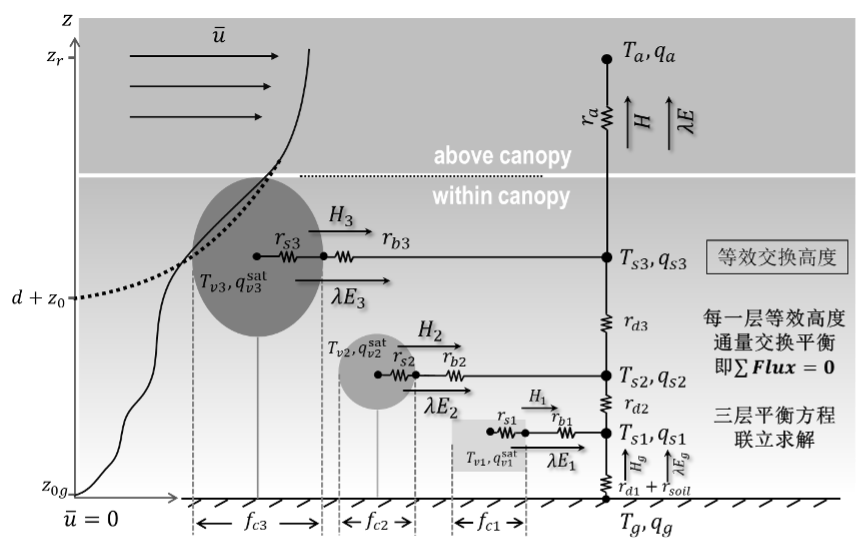
\includegraphics{Figures/地表湍流交换过程/三层植被湍流交换示意图.png}
\caption{三层植被湍流交换示意图。}
\label{fig:三层植被湍流交换示意图}
\end{figure}
}


通过以上介绍可以看出,三维植被湍流交换与一维植被湍流交换最大的不同在于其计算的对象由原来单一植被扩展到多个分层植被,
阻抗网络发生变化,多种植被在同一环境下同时求解。在计算时,同一维植被一样,需要用到植被短波辐射吸收量和长波辐射吸收量,
此时利用章节 \ref{三维植被辐射传输模型} 和 \ref{三维植被长波辐射传输} 对三维植被辐射传输计算结果。整个植被冠层与大气的湍流交换同样采用相似性理论进行求解,
其求解过程如图 \ref{fig:三维植被湍流交换模型计算流程图}所示。
{
\begin{figure}[]
\centering
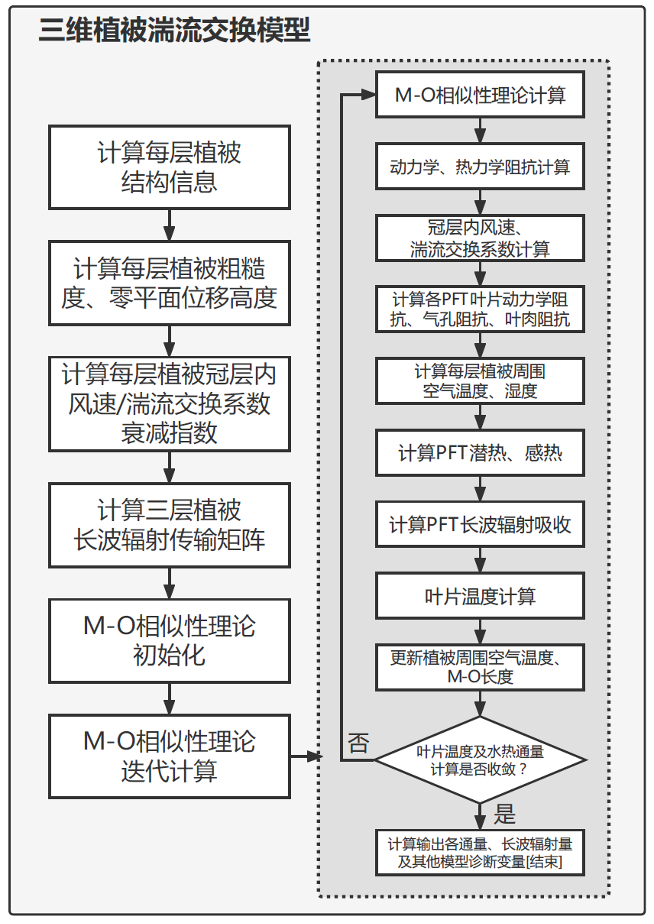
\includegraphics{Figures/地表湍流交换过程/三维植被湍流交换模型计算流程图.png}
\caption{三维植被湍流交换模型计算流程图。}
\label{fig:三维植被湍流交换模型计算流程图}
\end{figure}
}




\section{饱和水汽压(比湿)及其随温度的变化}\label{饱和水汽压(比湿)及其随温度的变化}
饱和水汽压 ($e_{sat}^T$, Pa) 与饱和比湿 ($q_{sat}^T$, kg/kg) 只依赖于温度 ($T$,\textcelsius) 的变化,
其计算方案采用\citet{flatau1992polynomial} 提出的八阶多项式拟合法:
\begin{equation}
e_{s a t}^{T}=100\left[a_{0}+a_{1} T+\cdots+a_{n} T^{n}\right]
\end{equation}
\begin{equation}
\frac{d e_{s a t}^{T}}{d T}=100\left[b_{0}+b_{1} T+\cdots+b_{n} T^{n}\right]
\end{equation}
\begin{equation}
q_{s a t}^{T}=\frac{0.622 e_{s a t}^{T}}{P_{atm}-0.378 e_{s a t}^{T}}
\end{equation}
\begin{equation}
\frac{d q_{{sat }}^{T}}{d T}=\frac{0.622 P_{atm}}{\left(P_{atm}-0.378 e_{{sat }}^{T}\right)^{2}} \frac{d e_{{sat }}^{T}}{d T}
\end{equation}
其中固态水($-75$\textcelsius$\le T<0$\textcelsius)与液态水($0$\textcelsius $\le T\le100$\textcelsius)情形对应的拟合系数见
表 \ref{tab:e_sat_T的拟合系数} 和 \ref{tab:de_sat_dT的拟合系数}。
% Please add the following required packages to your document preamble:
% \usepackage{booktabs}
\begin{table}[]
\centering
\caption{$e_{sat}^T$的拟合系数。}
\label{tab:e_sat_T的拟合系数}
\begin{tabular}{@{}lcc@{}}
\toprule
     &  液态水  & 固态水                         \\ \midrule
$a_0$ & 6.11213476        & 6.11123516       \\
$a_1$ & $\rm 4.44007856 \times 10^{-1}$   & $\rm 5.03109514 \times 10^{-1}$  \\
$a_2$ & $\rm 1.43064234 \times 10^{-2}$   & $\rm 1.88369801 \times 10^{-2}$  \\
$a_3$ & $\rm 2.64461437 \times 10^{-4}$   & $\rm 4.20547422 \times 10^{-4}$  \\
$a_4$ & $\rm 3.05903558 \times 10^{-6}$   & $\rm 6.14396778 \times 10^{-6}$  \\
$a_5$ & $\rm 1.96237241 \times 10^{-8}$   & $\rm 6.02780717 \times 10^{-8}$  \\
$a_6$ & $\rm 8.92344772 \times 10^{-11}$  & $\rm 3.87940929 \times 10^{-10}$ \\
$a_7$ & $\rm -3.73208410 \times 10^{-13}$ & $\rm 1.49436277 \times 10^{-12}$ \\
$a_8$ & $\rm 2.09339997 \times 10^{-16}$  & $\rm 2.62655803 \times 10^{-15}$ \\ \bottomrule
\end{tabular}
\end{table}

% Please add the following required packages to your document preamble:
% \usepackage{booktabs}
\begin{table}[]
\centering
\caption{$\frac{d e_{sat}^T}{d T}$ 的拟合系数。}
\label{tab:de_sat_dT的拟合系数}
\begin{tabular}{@{}lcc@{}}
\toprule
     &  液态水  & 固态水                         \\ \midrule
$b_0$ & $\rm 4.44017302 \times 10^{-1}$   & $\rm 5.03277922 \times 10^{-1}$  \\
$b_1$ & $\rm 2.86064092 \times 10^{-2}$  & $\rm 3.77289173 \times 10^{-2}$  \\
$b_2$ & $\rm 7.94683137 \times 10^{-4}$   & $\rm 1.26801703 \times 10^{-3}$  \\
$b_3$ & $\rm 1.21211669 \times 10^{-5}$   & $\rm 2.49468427 \times 10^{-5}$  \\
$b_4$ & $\rm 1.03354611 \times 10^{-7}$   & $\rm 3.13703411 \times 10^{-7}$  \\
$b_5$ & $\rm 4.04125005 \times 10^{-10}$  & $\rm 2.57180651 \times 10^{-9}$  \\
$b_6$ & $\rm -7.88037859 \times 10^{-13}$ & $\rm 1.33268878 \times 10^{-11}$ \\
$b_7$ & $\rm -1.14596802 \times 10^{-14}$ & $\rm 3.94116744 \times 10^{-14}$ \\
$b_8$ & $\rm 3.81294516 \times 10^{-17}$  & $\rm 4.98070196 \times 10^{-17}$ \\\bottomrule
\end{tabular}
\end{table}

\chapter{降水与地表的能量交换}
%\addcontentsline{toc}{chapter}{降水与地表的能量交换}

%\begin{降水与地表的能量交换}
雨水与地表/植被之间存在温度差异,当降水发生时,它们之间可发生能量交换(雨水感热)。
\citet{wei2014impact} 表明,虽然在气候尺度上此能量交换的量级很小,但它可通过改变大气环流影响不同地区的气候特征,
故在气候模式中不可被忽略。下面给出雨水感热的计算方案。

\section{雨水温度}\label{雨水温度}
已有研究(如\citet{anderson1998moored})表明,
雨水温度非常接近于大气湿球温度,故这里雨水温度由湿球温度近似。根据湿球温度定义有如下关系:
\begin{equation}
C_{p a}\left(T_{w b}-T\right)=\lambda_{v}\left(r-r_{s a t}^{T_{w b}}\right)
\end{equation}
其中$C_{pa}$表示干空气的比热容(J/kg/K),$T_{wb}$表示大气湿球温度(K),
$T$表示大气环境温度(K),$r$表示混合比,$r_{sat}^{T_{wb}}$表示$T_{wb}$温度下的饱和混合比,
$\lambda_v$表示液态水的蒸发潜热(J/kg)。于是,取$T_{wb}$的初始值$T_{wb}^{\left(0\right)}=T$,
$T_{wb}$可通过如下过程进行迭代求解:
\begin{enumerate}
    \item 由章节 \ref{饱和水汽压(比湿)及其随温度的变化} 计算$T_{wb}^{\left(n\right)}$温度下的饱和比湿$q_{sat}^{T_{wb}^{\left(n\right)}}$;
    \item 通过混合比和比湿的换算关系($r=\frac{q}{1-q}$),计算混合比$r$与$r_{sat}^{T_{wb}^{\left(n\right)}}$;
    \item 由上述关系更新湿球温度:$T_{wb}^{\left(n\right)\ast}=T+\frac{\lambda_v}{C_{pa}}\left(r-r_{sat}^{T_{wb}^{\left(n\right)}}\right)$;
    \item 取更新前后湿球温度的平均值作为新一步的湿球温度:$T_{wb}^{\left(n+1\right)}=\left(T_{wb}^{\left(n\right)}+T_{wb}^{\left(n\right)\ast}\right)/2.0$。
\end{enumerate}
将上述过程迭代6次($n=0$,$\ldots$,5),作为最终的湿球温度$T_{wb}$。


当$T>T_f+2.5$K时,降水完全为液态水,可取雨水温度$T_p=T_{wb}$,否则$T_p$需根据降水的固态与液态比例进行调整。
根据“Snow Hydrology”(1956)中的实验结果,液态水占总降水的比例$f_{pl}$可按如下方式定义:
当$T_f+2.0K<T\le T_f+2.5K$时,$f_{pl}=0.4$ \\
当$T_f<T\le T_f+2.0K$时,$f_{pl}=-54.632+0.2T$ \\
当$T\le T_f$时,$f_{pl}=0$ \\
于是,当$T\le T_f+2.5K$且$f_{pl}>0$时,$T_p=T_f-\sqrt{\frac{1}{f_{pl}}-1}/100$,
否则当降水完全为固态时,$T_p=min{\left(T_f,T_{wb}\right)}$。\\
\section{植被/地表的雨水感热}\label{植被地表的雨水感热}
当地表有植被覆盖时,植被叶片与雨水的能量交换 ($\rm W/m^2$) 分别计算如下:
\begin{equation}
H_{p r c v}=C_{p l} q_{p l}\left(T_{p}-T_{v}\right)+C_{p i} q_{p i}\left(T_{p}-T_{v}\right)
\end{equation}

其中$C_{pl}$与$C_pi$分别表示液态水与固态水的比热容(J/kg/K),
$q_{pl}$与$q_{pi}$分别表示植被冠层对液态水和固态水的截流率(mm H2O/s)(计算见章节\ref{植被冠层截留})。


地表与雨水的能量交换 ($\rm W/m^2$) 为:
\begin{equation}
H_{p r c g}=C_{p l} p_{l}\left(T_{p}-T_{g}\right)+C_{p i} p_{i}\left(T_{p}-T_{g}\right)
\end{equation}
其中$p_l$与$p_i$分别表示落到地面的液态水与固态水降水率(mm H2O/s),
当有植被覆盖时,$p_l$与$p_i$为直接穿透植被冠层的降水率与沿叶茎流出冠层的降水率之和(计算见章节\ref{植被冠层截留})。


\chapter{植被叶片温度计算}\label{植被叶片温度计算}
%\addcontentsline{toc}{chapter}{植被叶片温度计算}
\begin{mymdframed}{代码}
本节对应的代码文件为\texttt{MOD\_LeafTemperature.F90}。
\end{mymdframed}
%\begin{植被叶片温度计算}

假设植被冠层的比热容很小,可忽略不计,则叶片能量平衡方程为:
\begin{equation}\label{FT_V}
F\left(T_{v}\right):=S_{v}+L_{v}\left(T_{v}\right)-H_{v}\left(T_{v}\right)-\lambda E_{v}\left(T_{v}\right)+H_{p r c v}\left(T_{v}\right)=0
\end{equation}
其中$S_v$表示叶片吸收的净太阳辐射(见章节~\ref{短波吸收辐射通量}),
$L_v$表示叶片吸收的净长波辐射。$T_v$可通过对方程 (\ref{FT_V}) 实施牛顿迭代法进行求解,迭代公式为:
\begin{equation}
\Delta T_{v}=-\frac{F\left(T_{v}^{(n)}\right)}{F^{\prime}\left(T_{v}^{(n)}\right)}
\end{equation}
其中$\Delta T_v=T_v^{\left(n+1\right)}-T_v^{\left(n\right)}$,$n$代表迭代次数。
此外,因为植被湍流通量与叶片温度相互耦合,故在温度迭代求解过程中,湍流通量也随之更新。因此,本章节与前面植被湍流计算章节有部分重复,可对照参考(章节~\ref{一维植被湍流交换模型})。

在能量平衡方程中,$S_v$不依赖于温度的变化,其表达式在章节~\ref{短波吸收辐射通量}中已经给出。
$L_v$可计算如下(假设植被叶片部分发射率为1):
\begin{equation}
L_{v}=\left(1-\tau_{v}\right)\left(L ^\downarrow+\varepsilon_{g} \sigma T_{g}^{4}-2 \sigma T_{v}^{4}\right) + \left( 1- \varepsilon_{g} \right )\left(1-\varepsilon_{v} \right)\varepsilon_{v} L^\downarrow + \left( 1- \varepsilon_{g} \right ) \varepsilon_{v}^2 \sigma T_{v}^4
\end{equation}
即植被吸收的净长波辐射等于植被吸收的来自大气和地表的长波辐射减去植被向大气和地表方向同时发出的长波辐射,其中$L^\downarrow$表示近地面大气下行长波辐射,$\varepsilon_g=0.96$表示地面的长波辐射发射率,$\tau_{v}$表示长波辐射直接穿过植被冠层的比例(见章节~\ref{长波净辐射通量}),植被整体的发射率可计算为$\varepsilon_v=1-\tau_v$。$L_v$对叶片温度的变化率如下:
\begin{equation}
\begin{aligned}
 \frac{\partial L_{v}}{\partial T_{v}} &= -8 \varepsilon_{v}\sigma T_{v}^{3} + 4 \left( 1- \varepsilon_{g} \right ) \varepsilon_{v}^2 \sigma T_{v}^3
\end{aligned}
\end{equation}
感热通量表达式$H_{v}$已在章节~\ref{一维植被湍流交换模型} 给出,其对温度的变化率为:
\begin{equation}
\frac{\partial H_{v}}{\partial T_{v}}=\rho_{atm} C_{pa} c_{v}^{h} \left( \frac{c_{a}^{h}}{c_{a}^{h} + c_{g}^{h} + c_{v}^{h}} + \frac{c_{g}^{h}}{c_{a}^{h} + c_{g}^{h} + c_{v}^{h}} \right)
\end{equation}
上式中变量$c_*^h$详见章节~\ref{一维植被湍流交换模型}。

对于水汽通量$E_{v}$,虽然其表达式也已在章节~\ref{一维植被湍流交换模型} 给出,但这里为了表达上的便利,我们引入对于植被表面蒸散发是否发生的判别因子$\delta$如下:
\begin{equation}
\delta=\left\{\begin{array}{cc}1 & \text { 当 }\ q_{s a t}^{T_{v}}>q_{s} \text { 即叶片蒸散发可以发生时 } \\ 0 & \text { 否则 }\end{array}\right.
\end{equation}
于是$c_v^w$可重新表达为如下形式:
\begin{equation}
c_{v}^{w}=\frac{1}{r_{v}}=\frac{\left[1-\delta\left(1-f_{wet}\right)\right](\text{LAI+SAI})}{r_{b}}+\left( 1 - f_{wet} \right)\delta\left( \frac{\rm LAI_{sun}}{r_{b} + r_{s,\rm sun}} + \frac{\rm LAI_{sha}}{r_{b} + r_{s,\rm sha}} \right)
\end{equation}
对于叶片的蒸腾通量计算为:
\begin{equation}
E_{vt} = -\frac{\rho_{atm}\left(1-f_{w e t}\right)\delta }{c_{a}^{w}+c_{g}^{w}+c_{v}^{w}}\left( \frac{\rm LAI_{sun}}{r_{b} + r_{s,\rm sun}} + \frac{\rm LAI_{sha}}{r_{b} + r_{s,\rm sha}} \right) \left[c_{a}^{w} q_{atm}+c_{g}^{w} q_{g}-\left(c_{a}^{w}+c_{g}^{w}\right) q_{s a t}^{T_{v}}\right] 
\end{equation}
其对温度的变化率为:
\begin{equation}
\frac{\partial E_{vt}}{\partial T_{v}} = \rho_{atm} \left(1-f_{w e t}\right) \delta \left( \frac{\rm LAI_{sun}}{r_{b} + r_{s, \rm sun}} + \frac{\rm LAI_{sha}}{r_{b} + r_{s,\rm sha}} \right)\frac{c_{a}^{w}+c_{g}^{w}}{c_{a}^{w}+c_{g}^{w}+c_{v}^{w}} \frac{d q_{s a t}^{T_{v}}}{d T_{v}}
\end{equation}
对于叶片的蒸发通量计算为:
\begin{equation}
E_{va} = -\frac{\rho_{atm}}{c_{a}^{w}+c_{g}^{w}+c_{v}^{w}} \frac{\left[1-\delta\left(1-f_{w e t}\right)\right](\text {LAI+SAI)}}{r_{b}}\left[c_{a}^{w} q_{atm}+c_{g}^{w} q_{g}-\left(c_{a}^{w}+c_{g}^{w}\right) q_{sat}^{T_{v}}\right]
\end{equation}
其对温度的变化率为:
\begin{equation}
\frac{\partial E_{va}}{\partial T_{v}} = \frac{\rho_{atm}\left[1-\delta\left(1-f_{w e t}\right)\right](\text {LAI+SAI})}{r_{b}} \frac{c_{a}^{w}+c_{g}^{w}}{c_{a}^{w}+c_{g}^{w}+c_{v}^{w}} \frac{d q_{s a t}^{T_{v}}}{d T_{v}}
\end{equation}

由于蒸发与蒸腾速率均受到一定限制,所以$E_{v}$将分别针对蒸发与蒸腾速率进行调整:\\
当$ E_{vt} \geq E_{vt,max}$ 即叶片最大蒸腾率(\unit{kg.m^{-2}.s^{-1}})时,
\begin{equation}
\begin{aligned}
E_{vt} &=  E_{vt, \max } \\[1ex] 
\frac{\partial E_{vt}}{\partial T_{v}} &= 0
\end{aligned}
\end{equation}
当$E_{va} \geq \frac{W_{can}}{\Delta t}$即达到叶片最大可蒸发通量(\unit{kg.m^{-2}.s^{-1}})时,
\begin{equation}
  \begin{aligned}
   E_{va} &= \frac{W_{can}}{\Delta t} \\[1ex] 
   \frac{\partial E_{va}}{\partial T_{v}} &= 0
  \end{aligned}
\end{equation}
于是对于叶片的总水汽通量:
\begin{equation}
   E_{v} = E_{vt}+E_{va} 
\end{equation}
对温度的变化率为:
\begin{equation}
   \frac{\partial E_{v}}{\partial T_{v}} = \frac{\partial E_{vt}}{\partial T_{v}}+\frac{\partial E_{va}}{\partial T_{v}}
\end{equation}
雨水感热表达式$H_{prcv}$已在章节~\ref{植被地表的雨水感热} 给出,其对温度的变化率为:
\begin{equation}
\frac{\partial H_{prcv}}{\partial T_{v}}=-\left[C_{p l} q_{p l}+C_{p i} q_{p i}\right]
\end{equation}
基于以上表达式以及$T_v$的迭代公式,下面给出$T_v$以及植被湍流通量的求解流程:
\begin{enumerate}
    \item 给出植被冠层空气温度和比湿的初始猜测:$T_s=\frac{T_g+\theta_{atm}}{2}$,$q_s=\frac{q_g+q_{atm}}{2}$;
    \item 给出$U_c$的初始猜测如下:\\
    \begin{equation*}
    U_c= \begin{cases}
      0,  & \theta_{v,atm}-\theta_{v,s}\geq0 \text{ 即稳定条件下;} \\
      0.5, & \theta_{v,atm}-\theta_{v,s}<0 \text{ 即不稳定条件下;}
     \end{cases}
    \end{equation*}
    \item 通过$R_{ib}$给出$L$的初始猜测;
    \item 迭代以下过程以求得$T_v$以及植被湍流通量:\\
    a. 通过风速、温度、比湿的微分方程(M-O相似性理论)积分结果求得$u_\ast$、$\theta_\ast$、$q_\ast$ \\
    b. 计算植被冠层空气与大气之间的阻抗系数$r_{am}$、$r_{ah}$、$r_{aw}$ \\
    c. 计算叶片边界层阻抗$r_b$ \\
    d. 计算植被冠层空气与地表之间的阻抗系数$r_{ah}^\prime$、$r_{aw}^\prime$ \\
    e. 计算阳叶、阴叶气孔阻抗$r_{s,sun}$和$r_{s,sha}$ \\
    f. 分别计算叶片吸收的长波辐射、感热通量、潜热通量和雨水感热$L_v$、$H_{v}$、$\lambda E_{v}$、$H_{prcv}$ \\
    g. 若前后两次迭代过程中潜热通量的符号发生变化($\lambda E_{v}^{\left(n\right)}\times\lambda E_{v}^{\left(n+1\right)}<0$),
    则在该次迭代计算温度时,潜热通量的量级限制为原量级的10\%,由此产生的能量差最后将加到感热通量中 \\
    h. 计算温度变化$\Delta T_v$,并由此更新$T_v^{\left(n+1\right)}=\Delta T_v^{\left(n\right)}+T_v^{\left(n\right)}$。在每次迭代过程中,对于温度的变化作出如下两个限制:
    (1)温度的变化不得超过1 K,若超过,则强制其变化只有1K;
    (2)若本次迭代温度变化的方向与上一次变化的方向相反,则本次温度的变化将取为两次变化的平均值(若$\Delta T_v^{\left(n-1\right)} \cdot \Delta T_v^{\left(n\right)}<0$,则$\Delta T_v^{\left(n\right)}=\left(\Delta T_v^{\left(n-1\right)}+\Delta T_v^{\left(n\right)}\right)/2$)\\
    由温度调整所带来的能量平衡误差最后将加到感热通量中\\
    i. 更新饱和比湿$q_{sat}^{T_v}$及其对$T_v$的变化率 \\
    j. 更新植被冠层空气温度和比湿$T_s$, $q_s$ \\ 
    k. 更新特征位温$\theta_\ast$和特征比湿$q_\ast$ \\
    l. 更新特征虚位温$\theta_{v\ast}$ \\
    m. 更新大气风速$V_a\left(U_c\right)$ \\
    n. 计算新一步$L$,并计算$\zeta$,根据稳定性条件限制$\zeta$的取值范围 \\
    o. 根据限制条件后的$\zeta$重新计算$L=\frac{z_{atm,m}-d}{\zeta}$ \\
    p. 判断$L$与上一步迭代相比是否改变符号,若改变符号累计超过4次,则视为中性条件,
    $L$取固定值$L=\frac{z_{atm,m}-d}{-0.01}$,以避免在稳定与不稳定条件之间来回变化。\\
    q. 判断迭代停止条件:若迭代过程中满足下列全部条件或迭代次数已超过40次,则迭代停止
    \begin{equation}
        \begin{array}{l}\max\left( \sqrt{\left[F^{(n+1)}-F^{(n)}\right]^{\ast\ast2}}, \sqrt{\left[F^{(n)}-F^{(n-1)}\right]^{\ast\ast2}} \right) \leq 0.1 \\[1.5ex] 
        \max\left( \sqrt{\left(\Delta T_{v}^{(n)}\right)^{2}}, \sqrt{\left(\Delta T_{v}^{(n-1)}\right)^{2}} \right) \leq 0.01\end{array}
    \end{equation}
    其中$\left[\bullet\right]^{\ast\ast2}$表示各个相同能量项相邻时间步变化量(相减后)的平方和
    \item 由最终叶片温度更新植被表面与植被冠层空气之间的潜热通量,其中蒸发量不得超过植被截水量$W_{can}$,蒸腾率不得超过最大蒸腾率$ E_{vt,max}$,若超过则蒸发(腾)率强制取为最大蒸发(腾)率,由此产生的能量差最后将加到感热通量中
    \item 由最终叶片温度更新植被表面与植被冠层空气之间的感热通量以及上述因为潜热与温度的调整导致的能量误差之和
    \item 由最终叶片温度更新植被冠层的雨水感热
    \item 计算总动量通量为
    \begin{equation}
    \begin{aligned}
    \tau_{x} &=- \rho_{atm} \frac{u_{atm}}{r_{a m}} \\[1ex] 
    \tau_{y} & =- \rho_{atm} \frac{v_{atm}}{r_{am}}
    \end{aligned}
    \end{equation}
    \item 计算有植被覆盖下的地面感热通量$H_{g}$和潜热通量$\lambda E_{g}$及其对地面温度的变化率,
    并给出地表总感热通量$H_g$和潜热通量$\lambda E_g$随地面温度变化率
    \item 计算植被覆盖下地表吸收的下行长波辐射$L_{v}^\downarrow$和返回大气的上行长波辐射$L_v ^\uparrow$:
    \begin{equation}
        L_{v} ^\downarrow =  \tau_{v} L ^\downarrow+\varepsilon_{v}\sigma \left (T_{v}^{(n - 1)}\right)^3\left( T_{v}^{(n - 1)} + 4\Delta T_{v}^{(n - 1)} \right)\\
    \end{equation}
    \begin{equation}
    \begin{aligned}
        L_{v}^ \uparrow &=  \tau_{v} \varepsilon_{g} \sigma T_{g}^{4}+ \varepsilon_{v}\sigma \left ( T_{v}^{(n - 1)}\right )^3\left( T_{v}^{(n - 1)} + 4\Delta T_{v}^{(n - 1)} \right) \\[1ex]
&\mathrel{\phantom{=}} + \left ( 1- \varepsilon_{g} \right)\mu_{v}^2 L ^\downarrow + \left ( 1- \varepsilon_{g} \right) \mu_{v} \varepsilon_{v} \sigma \left (T_{v}^{(n - 1)}\right) ^4 \\[1ex]
&\mathrel{\phantom{=}} + 4 \left ( 1- \varepsilon_{g} \right) \mu_{v} \varepsilon_{v} \sigma \left (T_{v}^{(n - 1)}\right)^3 \Delta T_{v}^{(n - 1)}
    \end{aligned}
    \end{equation}
    \item 计算地表2 m温度与比湿$T_{2m}$、$q_{2m}$。
\end{enumerate}

\chapter{雪盖土壤热力过程}
%\addcontentsline{toc}{chapter}{雪盖土壤热力过程}

%\begin{雪盖土壤热力过程}

在雪盖和土壤中,热力过程主要根据热传导第二定律进行描述。假设雪盖土壤无水平物质能量交换,则其垂直方向上的一维能量平衡方程如下:
\begin{equation}\label{eq:1d_energy_balance}
c \frac{\partial T}{\partial t}=-\frac{\partial F}{\partial z}
\end{equation}
其中$c$表示雪盖或土壤的体积热容量(\unit{J.m^{-3}.K^{-1}}),$T$表示雪盖土壤温度 (K),$t$表示时间(s),$z$表示雪盖高度或土壤深度 (m),
F表示垂直方向的热传导通量,方向向上为正(\unit{W.m^{-2}}),表达式为$F=-\lambda\frac{\partial T}{\partial z}$,$\lambda$表示热力传导率(\unit{W.m^{-1}.K^{-1}})。
将方程(\ref{eq:1d_energy_balance})进行离散,并结合上边界由大气输送到雪盖土壤表面的热通量$h_s$以及下边界土壤底层的零热通量,
即可求出雪盖土壤的温度扩线,之后再根据相态变化条件对温度进行进一步调整。


\section{温度求解的数值格式}\label{温度求解的数值格式}
在离散上述能量平衡方程时,土壤被划分为10层。每一层土壤的中心深度$z_i$(m)定义为:
\begin{equation}
z_{i}=f_{s} \exp [0.5(i-0.5)]-1
\end{equation}
%
其中尺度因子$f_s=0.025$。这里采用指数定义可以保证土壤接近表面时得到更细的分层,因为土壤水梯度在接近表面时非常大。基于此定义,每一层土壤的厚度$\Delta z_i$ (m)可计算为:
\begin{equation}
\Delta z_{i}=\left\{\begin{array}{ll}0.5\left(z_{1}+z_{2}\right) & i=1 \\ 0.5\left(z_{i+1}-z_{i-1}\right) & i=2 \ldots 9 \\ z_{10}-z_{9} & i=10\end{array}\right.
\end{equation}
相邻两层土壤交界处的深度$z_{h,i}$ (m)可计算为:
\begin{equation}
z_{h, i}=\left\{\begin{array}{ll}0.5\left(z_{i}+z_{i+1}\right) & i=1 \ldots 9 \\ z_{10}+0.5 \Delta z_{10} & i=10\end{array}\right.
\end{equation}



雪盖位于土壤之上,可根据其厚度划分为至多5层。为与土壤层编号一致,
这里与土壤表层相邻的雪层记为第0层,逐渐向上依次记为第 -1 层直至至多为第 -4 层。
记$snl$为划分的雪层总层数的相反数,则最上层雪层即为第$snl+1$层。雪层划分方案如下:\\
当$z_{sno}<0.01$时,$snl=0$,这时积雪较少,不单独划分为层;\\
当$0.01\le z_{sno}\le0.03$时,\\
\begin{equation}
\left\{\begin{array}{c}s n l=-1 \\ \Delta z_{0}=z_{sno}\end{array}\right.
\end{equation}
当$0.03<z_{sno}\le0.04$时,
\begin{equation}
\left\{\begin{array}{c}s n l=-2 \\ \Delta z_{-1}=z_{sno} / 2 \\ \Delta z_{0}=\Delta z_{-1}\end{array}\right.
\end{equation}
当$0.04<z_{sno}\le0.07$时,
\begin{equation}
\left\{\begin{array}{c}s n l=-2 \\ \Delta z_{-1}=0.02 \\ \Delta z_{0}=z_{sno}-\Delta z_{-1}\end{array}\right.
\end{equation}
当$0.12<z_{sno}\le0.18$时,
\begin{equation}
\left\{\begin{array}{c}s n l=-3 \\ \Delta z_{-2}=0.02 \\ \Delta z_{-1}=0.05 \\ \Delta z_{0}=z_{sno}-\Delta z_{-2}-\Delta z_{-1}\end{array}\right.
\end{equation}
当$0.18<z_{sno}\le0.29$时,
\begin{equation}
\left\{\begin{array}{c}s n l=-4 \\ \Delta z_{-3}=0.02 \\ \Delta z_{-2}=0.05 \\ \Delta z_{-1}=\left(z_{sno}-\Delta z_{-3}-\Delta z_{-2}\right) / 2 \\ \Delta z_{0}=\Delta z_{-1}\end{array}\right.
\end{equation}
当$0.29<z_{sno}\le0.41$时,
\begin{equation}
\left\{\begin{array}{c}s n l=-4 \\ \Delta z_{-3}=0.02 \\ \Delta z_{-2}=0.05 \\ \Delta z_{-1}=0.11 \\ \Delta z_{0}=z_{sno}-\Delta z_{-2}-\Delta z_{-1}\end{array}\right.
\end{equation}
当$0.41<z_{sno}\le0.64$时,
\begin{equation}
\left\{\begin{array}{c}s n l=-5 \\ \Delta z_{-4}=0.02 \\ \Delta z_{-3}=0.05 \\ \Delta z_{-2}=0.11 \\ \Delta z_{-1}=\left(z_{sno}-\Delta z_{-3}-\Delta z_{-2}\right) / 2 \\ \Delta z_{0}=\Delta z_{-1}\end{array}\right.
\end{equation}
当$z_{sno}>0.64$时,
\begin{equation}
\left\{\begin{array}{c}s n l=-5 \\ \Delta z_{-4}=0.02 \\ \Delta z_{-3}=0.05 \\ \Delta z_{-2}=0.11 \\ \Delta z_{-1}=0.23 \\ \Delta z_{0}=z_{sno}-\Delta z_{-3}-\Delta z_{-2}-\Delta z_{-1}\end{array}\right.
\end{equation}
$z_{h,0}=0$为雪盖底层与土壤表层交界处的高度。将此交界面以上的高度定义为负值,则每一层雪的中心高度$z_i$(m)与相邻两层雪交界处的高度$z_{h,i}$(m)计算为:
\begin{equation}
\begin{aligned}
z_{i} &= z_{h, i}-0.5 \Delta z_{i} \quad i=0, \ldots, snl+1 \\ 
z_{h, i} &= z_{h, i+1}-\Delta z_{i+1}  \quad i=-1, \ldots, snl
\end{aligned}
\end{equation}
注意,在计算雪盖土壤温度之前,若有降雪发生($p_i>0$)且无雪盖分层($snl=0$),则此时需通过下式判断第一层雪能否形成:
\begin{equation}
\begin{aligned}
z_{sno} &= z_{sno}+\frac{p_{i} \Delta t}{\rho_{\text {sno,new }}} \\ 
W_{sno} &= W_{sno}+p_{i} \Delta t
\end{aligned}
\end{equation}
其中$\rho_{sno,new}$表示新降的干雪密度(\unit{kg.m^{-3}}),计算方案为~\citep{anderson1976point}:
\begin{equation}
\rho_{sno, new}=\begin{cases}
169 & \text { 当 }\ T_{atm}>T_{f}+2.0 \\ 
50+1.7\left(T_{atm}-T_{f}+15\right)^{1.5}  & \text { 当 }\ T_{f}-15.0<T_{atm} \leq T_{f}+2.0 \\ 
50 & \text { 当 }\ T_{atm} \leq T_{f}-15.0
\end{cases}
\end{equation}
若此时$z_{sno} \geq 0.01$,则按如上方式对积雪进行分层,且每一层雪的温度取为$T_p$,液态水含量取为0,固态水含量按雪层厚度权重分配$W_{sno}$。若之前已有雪层且此时有降雪发生,则第一层雪的相关物理量作如下更新:
\begin{equation}
w_{ice, snl+1}=w_{ice, snl+1}+p_{i} \Delta t
\end{equation}
\begin{equation}
\Delta z_{snl+1}=\Delta z_{snl+1}+\frac{p_{i} \Delta t}{\rho_{sno, new}}
\end{equation}
\begin{equation}
z_{snl+1}=z_{h, snl+1}-0.5 \Delta z_{snl+1}
\end{equation}
\begin{equation}
z_{h, snl}=z_{h, snl+1}-\Delta z_{snl+1}
\end{equation}
雪盖土壤垂直分层及其热传导过程示意图见图~\ref{fig:雪盖土壤垂直分层及其热传导过程示意图}。其中土壤热力学状态变量
(如雪盖土壤温度$T_i$,热力传导率$\lambda_i$,体积比热容$c_i$等)定义在每一层的中间深度,从第$i+1$层到第$i$层的热传导通量$F_i$定义在两层的交界处,它可离散为:
\begin{equation}
F_{i}=\lambda\left[z_{h, i}\right] \frac{T_{i}-T_{i+1}}{z_{i}-z_{i+1}}
\end{equation}
其中$\lambda\left[z_{h,i}\right]$表示第$i+1$层与第 $i$ 层交界处的热力传导率。求解$\lambda\left[z_{h,i}\right]$时,
假设从第$i+1$层到第$i$层的热传导通量等于从第$i+1$层到第$i+1$层与第$i$层交界层的热传导通量,又等于从交接层到第$i$层的热传导通量,即
\begin{equation}
\lambda\left[z_{h, i}\right] \frac{T_{i}-T_{i+1}}{z_{i}-z_{i+1}}=\lambda_{i+1} \frac{T_{m}-T_{i+1}}{z_{h, i}-z_{i+1}}=\lambda_{i} \frac{T_{i}-T_{m}}{z_{i}-z_{h, i}}
\end{equation}
即可通过后两项解出第$i+1$层与第$i$层交界处的温度$T_m$;再将$T_m$代回,通过前两项即可解出$\lambda\left[z_{h,i}\right]$为:
\begin{equation}
\lambda\left[z_{h, i}\right]=\begin{cases}
\frac{\lambda_{i} \lambda_{i+1}\left(z_{i}-z_{i+1}\right)}{\lambda_{i}\left(z_{h, i}-z_{i+1}\right)+\lambda_{i+1}\left(z_{i}-z_{h, i}\right)} & i=snl+1, \ldots, 9 \\ 
0 & i=10
\end{cases}
\end{equation}
特殊地,对于土壤与雪盖的交界面,为防止最下层雪盖厚度过大导致$\lambda\left[z_{h,i}\right]$计算不准,
当$i=0$且$\left(z_{i+1}-z_{h,i}\right)<\left(z_{h,i}-z_i\right)$时,$\lambda\left[z_{h,i}\right]$重新计算为:
\begin{equation}
\lambda\left[z_{h,i}\right]=\frac{2 \lambda_{i} \lambda_{i+1}}{\lambda_{i}+\lambda_{i+1}} \geq 0.5 \lambda_{i+1}
\end{equation}
{
\begin{figure}[]
\centering
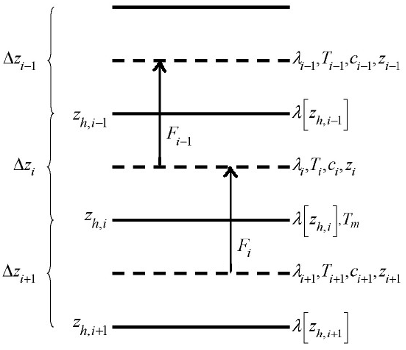
\includegraphics{Figures/雪盖土壤热力过程/雪盖土壤垂直分层及其热传导过程示意图.png}
\caption{雪盖土壤垂直分层及其热传导过程示意图。}
\label{fig:雪盖土壤垂直分层及其热传导过程示意图}
\end{figure}
}


基于以上离散方案,第$i$层雪盖土壤的能量平衡方程可表达为:
\begin{equation}
\frac{c_{i} \Delta z_{i}}{\Delta t}\left(T_{i}^{n+1}-T_{i}^{n}\right)=F_{i}-F_{i-1}
\end{equation}
%
其中$\Delta t$表示积分时间步长,$n$表示积分步数。此方程采用Crank--Nicholson半隐式格式求解,既包含前一时刻已有的温度与热通量信息,又包含后一时刻的预报信息。于是此方程可写为如下形式:
\begin{equation}
\frac{c_{i} \Delta z_{i}}{\Delta t}\left(T_{i}^{n+1}-T_{i}^{n}\right)=\alpha\left(F_{i}^{n}-F_{i-1}^{n}\right)+(1-\alpha)\left(F_{i}^{n+1}-F_{i-1}^{n+1}\right)
\end{equation}
其中权重因子$\alpha=0.5$。此方程展开,即有
\begin{equation}
\begin{aligned} \frac{c_{i} \Delta z_{i}}{\Delta t}\left(T_{i}^{n+1}-T_{i}^{n}\right)=& 0.5\left\{\lambda\left[z_{h, i}\right] \frac{T_{i}^{n}-T_{i+1}^{n}}{z_{i}-z_{i+1}}-\lambda\left[z_{h, i-1}\right] \frac{T_{i-1}^{n}-T_{i}^{n}}{z_{i-1}-z_{i}}\right.\\ &\left.+\lambda\left[z_{h, i}\right] \frac{T_{i}^{n+1}-T_{i+1}^{n+1}}{z_{i}-z_{i+1}}-\lambda\left[z_{h, i-1}\right] \frac{T_{i-1}^{n+1}-T_{i}^{n+1}}{z_{i-1}-z_{i}}\right\} \end{aligned}
\end{equation}
将所有层雪盖土壤能量平衡方程联立,可形成关于预报变量$T_{i-1}^{n+1}$, $T_i^{n+1}$和$T_{i+1}^{n+1}$的三对角方程组形式:$r_i=a_iT_{i-1}^{n+1}+b_iT_i^{n+1}+c_iT_{i+1}^{n+1}$,
其中$a_i$, $b_i$, $c_i$分别为三对角矩阵中上三角、对角线和下三角位置中的元素。用追赶法解此方程组即可快速求得每一层雪盖土壤的温度$T_i^{n+1}$。


对于雪盖土壤的中间层($snl+1<i<10$),三对角矩阵中的系数表达如下:
\begin{equation}
\begin{aligned}
a_{i} &= -(1-\alpha) \frac{\Delta t}{c_{i} \Delta z_{i}} \frac{\lambda\left[z_{h, i-1}\right]}{z_{i}-z_{i-1}} \\ 
b_{i} &= 1+(1-\alpha) \frac{\Delta t}{c_{i} \Delta z_{i}}\left[\frac{\lambda\left[z_{h, i-1}\right]}{z_{i}-z_{i-1}}+\frac{\lambda\left[z_{h, i}\right]}{z_{i+1}-z_{i}}\right] \\ 
c_{i} &= -(1-\alpha) \frac{\Delta t}{c_{i} \Delta z_{i}} \frac{\lambda\left[z_{h, i}\right]}{z_{i+1}-z_{i}} \\
r_{i} &= T_{i}^{n}+\alpha \frac{\Delta t}{c_{i} \Delta z_{i}} \lambda\left[z_{h, i}\right] \frac{T_{i}^{n}-T_{i+1}^{n}}{z_{i}-z_{i+1}}-\lambda\left[z_{h, i-1}\right] \frac{T_{i-1}^{n}-T_{i}^{n}}{z_{i-1}-z_{i}}
\end{aligned}
\end{equation}
对于雪盖土壤的顶层和底层,需要考虑对应的边界条件:\\
(1) 对于雪盖土壤顶层($i=snl+1$),来自大气的热通量$h_s$将会进入到地表中,即
\begin{equation}
h_{s}^{n+1}=-\alpha F_{i-1}^{n}-(1-\alpha) F_{i-1}^{n+1}
\end{equation}
对$h_s^{n+1}$采用一阶泰勒展开近似,则顶层能量平衡方程变为:
\begin{equation}
\begin{split}
&\mathrel{\phantom{\approx}}\frac{c_{i} \Delta z_{i}}{\Delta t}\left(T_{i}^{n+1}-T_{i}^{n}\right)=h_{s}^{n+1}+\alpha F_{i}^{n}+(1-\alpha) F_{i}^{n+1} \\ 
&\approx h_{s}^{n}+\frac{\partial h_{s}}{\partial T_{i}}\left(T_{i}^{n+1}-T_{i}^{n}\right)+\alpha \lambda\left[z_{h, i}\right] \frac{T_{i}^{n}-T_{i+1}^{n}}{z_{i}-z_{i+1}}+(1-\alpha) \lambda\left[z_{h, i}\right] \frac{T_{i}^{n+1}-T_{i+1}^{n+1}}{z_{i}-z_{i+1}}
\end{split}
\end{equation}
于是,基于此方程可得雪盖土壤顶层的三对角矩阵系数为:
\begin{equation}
\begin{aligned}
a_{i} &= 0 \\ 
b_{i} &= 1+\frac{\Delta t}{c_{i} \Delta z_{i}}\left[(1-\alpha) \frac{\lambda\left[z_{h, i}\right]}{z_{i+1}-z_{i}}-\frac{\partial h_{s}}{\partial T_{i}}\right] \\
c_{i} &= -(1-\alpha) \frac{\Delta t}{c_{i} \Delta z_{i}} \frac{\lambda\left[z_{h, i}\right]}{z_{i+1}-z_{i}} \\
r_{i} &= T_{i}^{n}+\frac{\Delta t}{c_{i} \Delta z_{i}}\left[h_{s}^{n}-\frac{\partial h_{s}}{\partial T_{i}} T_{i}^{n}+\alpha \lambda\left[z_{h, i}\right] \frac{T_{i}^{n}-T_{i+1}^{n}}{z_{i}-z_{i+1}}\right]
\end{aligned}
\end{equation}
这里进入到地表的热通量$h_s$(\unit{W.m^{-2}})具体表达为:
\begin{equation}
\begin{aligned}
h_{s} &= S_{g}+L_{g}\left(T_{g}\right)-H_{g}\left(T_{g}\right)-\lambda E_{g}\left(T_{g}\right)+H_{p r c g}\left(T_{g}\right) \\
\frac{\partial h_{s}}{\partial T_{i}} &= \frac{\partial L_{g}}{\partial T_{i}}-\frac{\partial H_{g}}{\partial T_{i}}-\frac{\partial \lambda E_{g}}{\partial T_{i}}+\frac{\partial H_{p r c g}}{\partial T_{i}}
\end{aligned}
\end{equation}
其中$S_g$和$L_g$分别表示地表吸收的净太阳辐射和净长波辐射(\unit{W.m^{-2}})。$h_s$中的各个能量组份已在前面各节有所介绍,这里对于$L_g$的计算给予补充:
\begin{equation}
L_{g}=L_{p g} \downarrow+\varepsilon_{g} L_{b g} \downarrow-L_{g} \uparrow
\end{equation}
其中$L_{pg}\downarrow$表示植被覆盖下地表吸收的下行长波辐射(见章节~\ref{长波净辐射通量}),$L_{bg}\downarrow$表示无植被覆盖下到达地表的下行长波辐射:
\begin{equation}
L_{b g} \downarrow=\left(1-f_{ sig }\right) L \downarrow
\end{equation}
$L_g\uparrow$表示地表发出的上行长波辐射:
\begin{equation}
L_{g} \uparrow=\varepsilon_{g} \sigma T_{g}^{4}
\end{equation}
另外,对于潜热通量系数$\lambda$,当雪盖土壤顶层不存在液态水时,$\lambda$取为升华潜热系数$\lambda_s$,即:
\begin{equation}
\lambda=\left\{\begin{array}{lr}\lambda_{s} & \text { 当 } w_{liq, s n l+1}=0 \text { 并且 } w_{ice, s n l+1}>0 \\ \lambda_{v} & \text { 其他情况 }\end{array}\right.
\end{equation}
其中$w_{liq,snl+1}$和$w_{ice,snl+1}$分别表示雪盖土壤顶层的液态水和固态水含量 (\unit{kg.m^{-2}},其计算见章节~\ref{sec:土壤水的运动})。

在模式中,地表温度$T_g$与$T_{snl+1}$取为同一值,但$T_{snl+1}$表示第一层雪盖或土壤的平均温度,与实际的$T_g$相比具有减弱的日变化幅度。
为改进这一缺陷,在求解第一层能量平衡方程时,其厚度$\Delta z_i$作以下调整,以求得更接近实际的$T_g$:
\begin{equation}
\Delta z_{i}=0.5\left[z_{i}-z_{h, i-1}+c_{a}\left(z_{i+1}-z_{h, i-1}\right)\right]
\end{equation}
其中调整参数$c_a=0.34$。\\
(2) 对于土壤底层($i=10$),假设热传导通量为0,则能量平衡方程变为:
\begin{equation}
\frac{c_{i} \Delta z_{i}}{\Delta t}\left(T_{i}^{n+1}-T_{i}^{n}\right)=-\alpha \lambda\left[z_{h, i-1}\right] \frac{T_{i-1}^{n}-T_{i}^{n}}{z_{i-1}-z_{i}}-(1-\alpha) \lambda\left[z_{h, i-1}\right] \frac{T_{i-1}^{n+1}-T_{i}^{n+1}}{z_{i-1}-z_{i}}
\end{equation}
于是,基于此方程可得土壤底层的三对角矩阵系数为:
\begin{equation}
\begin{aligned}
a_{i} &= -(1-\alpha) \frac{\Delta t}{c_{i} \Delta z_{i}} \frac{\lambda\left[z_{h, i-1}\right]}{z_{i}-z_{i-1}} \\
b_{i} &= 1+(1-\alpha) \frac{\Delta t}{c_{i} \Delta z_{i}} \frac{\lambda\left[z_{h, i-1}\right]}{z_{i}-z_{i-1}} \\
c_{i} &= 0 \\
r_{i} &= T_{i}^{n}-\alpha \frac{\Delta t \lambda\left[z_{h, i-1}\right]}{c_{i} \Delta z_{i}} \frac{T_{i-1}^{n}-T_{i}^{n}}{z_{i-1}-z_{i}}
\end{aligned}
\end{equation}

下面给出各层雪盖土壤的热力传导率$\lambda_i$与体积热容量$c_i$的计算方案:\\

根据~\citet{farouki1981thermal},土壤热力传导率$\lambda_i$ (\unit{W.m^{-1}.K^{-1}}, $i=1,\ldots,10$)的计算公式如下:

\begin{equation}
\lambda_{i}=\left\{\begin{array}{ll}K_{e, i} \lambda_{sat, i}+\left(1-K_{e, i}\right) \lambda_{d r y, i} & S_{r, i}>1 \times 10^{-7} \\ \lambda_{d r y, i} & S_{r, i} \leq 1 \times10^{-7}\end{array}\right.
\end{equation}
其中,$\lambda_{sat,i}$与$\lambda_{dry,i}$分别是饱和土壤和干土壤的热力传导率,由地表参数数据集提供,$S_{r,i}$表示土壤相对于其饱和状态的潮湿程度:
\begin{equation}
S_{r, i}=\left(\frac{w_{liq, i}}{\rho_{liq} \Delta z_{i}}+\frac{w_{ice, i}}{\rho_{ice} \Delta z_{i}}\right) \frac{1}{\theta_{sat, i}} \leq 1
\end{equation}
$K_{e,i}$表示Kersten数,它是$S_{r,i}$的函数:
\begin{equation}
K_{e, i}=\left\{\begin{array}{ll}\log _{10} S_{r, i}+1 \geq 0 & \text{ 当 } T_{i} \geq T_{f} \text{ 时 } \\ S_{r, i} & \text{ 当 } T_{i}<T_{f} \text{ 时 }\end{array}\right.
\end{equation}
当$T_i<T_f$时,饱和土壤热力传导率$\lambda_{sat,i}$需根据已有$\lambda_{sat,i}$结合水和冰的热力传导率$\lambda_{liq}$,$\lambda_{ice}$进行调整:
\begin{equation}
\lambda_{sat, i}=\lambda_{sat, i}\left(\frac{\lambda_{ice}}{\lambda_{liq}}\right)^{\theta_{sat, i}\left(1-\frac{w_{liq, i}}{w_{liq, i}+w_{ice, i}}\right)}
\end{equation}
$\theta_{sat, i}$表示第$ i $层土壤的孔隙度。


根据 \citet{jordan1991one},雪盖热力传导率$\lambda_i$ (\unit{W.m^{-1}.K^{-1}}, $i=snl+1,\ldots,0$)的计算公式如下:
\begin{equation}
\lambda_{i}=\lambda_{a}+\left(7.75 \times 10^{-5} \rho_{sno, i}+1.105 \times 10^{-6} \rho_{sno, i}^{2}\right)\left(\lambda_{ice}-\lambda_{a}\right)
\end{equation}
其中$\lambda_a$表示空气的热力传导率(\unit{W.m^{-1}.K^{-1}}),$\rho_{sno,i}$表示第 $i$ 层雪的平均密度(\unit{kg.m^{-3}}):
\begin{equation}
\rho_{sno, i}=\frac{w_{liq, i}+w_{ice, i}}{\Delta z_{i}}
\end{equation}



根据 \citet{de1963thermal},土壤体积热容量$c_i$ (\unit{J.m^{-3}.K^{-1}}, $i=1, \ldots, 10$)的计算公式如下:
\begin{equation}
c_{i}=c_{s, i}\left(1-\theta_{sat, i}\right)+\frac{w_{ice, i}}{\Delta z_{i}} C_{pi}+\frac{w_{liq, i}}{\Delta z_{i}} C_{p l}
\end{equation}
其中$c_{s,i}$表示干土壤的体积热容量,由地表参数数据集提供。若地表有积雪但无雪层,则积雪的热容量也需考虑:
\begin{equation}
c_{i}=c_{s,i}\left(1-\theta_{sat, i}\right)+\frac{w_{ice, i}}{\Delta z_{i}} C_{pi}+\frac{w_{liq,i}}{\Delta z_{i}} C_{pl}+\frac{W_{sno}}{\Delta z_{i}} C_{pi}
\end{equation}
对于雪盖体积热容量$c_i$ (\unit{J.m^{-3}.K^{-1}}, $i=snl+1, \ldots, 0$),其计算公式为:
\begin{equation}
c_{i}=\frac{w_{ice, i}}{\Delta z_{i}} C_{pi}+\frac{w_{liq, i}}{\Delta z_{i}} C_{pl}
\end{equation}


\section{温度的相态变化调整}
通过解能量平衡方程组计算出下一时刻的雪盖土壤温度后,需要考虑相态变化过程对温度进行调整。在模式中,相态变化发生的条件为:\\
若$T_i^{n+1}>T_f$并且$w_{ice,i}>0$ \ \   \ \  \ \   固态水融化\\
若$T_i^{n+1}<T_f$并且$w_{liq,i}>0$  \ \   \ \  \ \         液态水冻结\\
一个特殊情况是,当土壤表面积雪存在$\left(W_{sno}>0\right)$但并无雪层$\left(snl=0,z_{sno}<0.01\right)$时,\\
若$T_1^{n+1}>T_f$      \ \   \ \  \ \                 积雪融化\\
以上三种情况下,$T_i^{n+1}$被调整为$T_f$。


相态变化的程度是由$T_i^{n+1}$调整为$T_f$后产生的能量冗余或亏损决定的。温度调整后,能量的冗余或亏损$H_i$ (\unit{W.m^{-2}})计算如下:
\begin{equation}
H_{i}=\begin{cases}
h_{s}^{n}+\frac{\partial h_{s}}{\partial T_{i}}\left(T_{f}-T_{i}^{n}\right)+\alpha F_{i}^{n}+(1-\alpha) F_{i}^{n+1}-\frac{c_{i} \Delta z_{i}}{\Delta t}\left(T_{f}-T_{i}^{n}\right) & i=snl+1 \\
\alpha\left(F_{i}^{n}-F_{i-1}^{n}\right)+(1-\alpha)\left(F_{i}^{n+1}-F_{i-1}^{n+1}\right)-\frac{c_{i} \Delta z_{i}}{\Delta t}\left(T_{f}-T_{i}^{n}\right) & snl+1<i<10 \\
-\alpha F_{i-1}^{n}-(1-\alpha) F_{i-1}^{n+1}-\frac{c_{i} \Delta z_{i}}{\Delta t}\left(T_{f}-T_{i}^{n}\right) & i=10
\end{cases}
\end{equation}
对应地,相态变化的质量调整量为$H_{m}=\frac{H_{i} \Delta t}{L_{f}}$,其中$L_f$表示固态水液化潜热(\unit{J.kg^{-1}})。当固态水融化条件被满足且$H_m>0$时,固态水含量被调整为:
\begin{equation}
w_{ice, i}^{n+1}=w_{ice, i}^{n}-H_{m} \geq 0
\end{equation}
当液态水冻结条件被满足且$H_m<0$时,固态水含量被调整为:
\begin{equation}
w_{ice, i}^{n+1}=\min{\left(w_{ice, i}^{n}-H_{m}, w_{liq, i}^{n}+w_{ice, i}^{n}\right)}
\end{equation}
以上情况液态水含量均被调整为:
\begin{equation}
w_{liq, i}^{n+1}=w_{liq, i}^{n}+w_{ice, i}^{n}-w_{ice, i}^{n+1} \geq 0
\end{equation}
若水分调节过程不足以消耗全部的能量冗余或填补全部的能量亏损,
则在相态变化过程之后再次进行能量结余计算:$ H_{i *}=H_{i}+\frac{L_{f}\left(w_{ice, i}^{n+1}-w_{ice, i}^{n}\right)}{\Delta t}$。
若$\left|H_{i\ast}\right|>0$,则此部分能量可用来再次暖化或冷却雪盖土壤层,温度调整如下:
\begin{equation}
T_{i}^{n+1}=\left\{\begin{array}{lr}T_{f}+\frac{\Delta t}{c_{i} \Delta z_{i}} H_{i *} /\left(1-\frac{\Delta t}{c_{i} \Delta z_{i}} \frac{\partial T_{s}}{\partial T_{i}}\right) & i=s n l+1 \\ T_{f}+\frac{\Delta t}{c_{i} \Delta z_{i}} H_{i *} & i \neq s n l+1 \\ T_{f} & w_{liq, i}^{n+1} \cdot w_{ice, i}^{n+1}>0\end{array}\right.
\end{equation}
对于特殊的土壤表面积雪融化的情形,当$H_m>0$时,雪水当量减少为
\begin{equation}
W_{sno}^{n+1}=W_{s no}^{n}-H_{m} \geq 0
\end{equation}
同样,雪的厚度减少为
\begin{equation}
z_{sno}^{n+1}=\frac{W_{sno}^{n+1}}{W_{sno}^{n}} z_{sno}^{n}
\end{equation}
若积雪融化不足以消耗全部的能量冗余,则剩余能量$H_{1\ast}$为
\begin{equation}
H_{1 *}=H_{1}+\frac{L_{f}\left(W_{sno}^{n+1}-W_{sno}^{n}\right)}{\Delta t}
\end{equation}
此时$H_{1\ast}$将作为新的$H_1$对第一层土壤进行上述相态变化计算。


综上,若发生土壤表面积雪融化的情形,则用于相态变化的能量累计$E$为:
\begin{equation}
E=\frac{L_{f}\left(W_{sno}^{n}-W_{sno}^{n+1}\right)}{\Delta t}+\sum_{i=1}^{10} \frac{L_{f}\left(w_{ice, i}^{n}-w_{ice, i}^{n+1}\right)}{\Delta t}
\end{equation}
否则,
\begin{equation}
E=\sum_{i=1}^{s n l+1} \frac{L_{f}\left(w_{ice, i}^{n}-w_{ice, i}^{n+1}\right)}{\Delta t}
\end{equation}
以上过程即是雪盖土壤温度计算的全部过程。得到$T_i^{n+1}$后,地表发出的上行长波辐射$L_g\uparrow$,感热通量$H_g$与潜热通量$\lambda E_g$需再做一次更新以作为输出的状态变量,
其中用于蒸发的水汽不能超过雪盖土壤顶层的总含水量$\left(w_{liq,snl+1}^{n+1}+w_{ice,snl+1}^{n+1}\right)/\Delta t$,
否则地表蒸发水汽取为$\left(w_{liq,snl+1}^{n+1}+w_{ice,snl+1}^{n+1}\right)/\Delta t$,产生的能量误差将加到感热通量上。

\section{雪的压实,雪层的合并和细分}
\subsection{雪层的建立}
\begin{mymdframed}{代码}
本节对应的代码文件为\texttt{MOD\_NewSnow.F90}。
\end{mymdframed}
在模式中,覆盖在地表的积雪被模拟为最多五层,具体取决于总积雪深度。积雪层数从上到下分别用$j = −4, −3, −2, −1, 0$编号。$j = 0$是靠近土壤表面的底层雪层,$j = snl + 1$是表层雪层,其中变量$snl$是积雪层数的负数。雪层的厚度表示为$\delta z_j$(m),雪层的深度$z_j$取为其上边界深度$\left[z_h\right]_{j-1}$和下边界深度$\left[z_h\right]_j$的平均值(\textcolor{red}{中位数?})(图~\ref{fig:模式中积雪雪层示意图})。
{
\begin{figure}[]
\centering
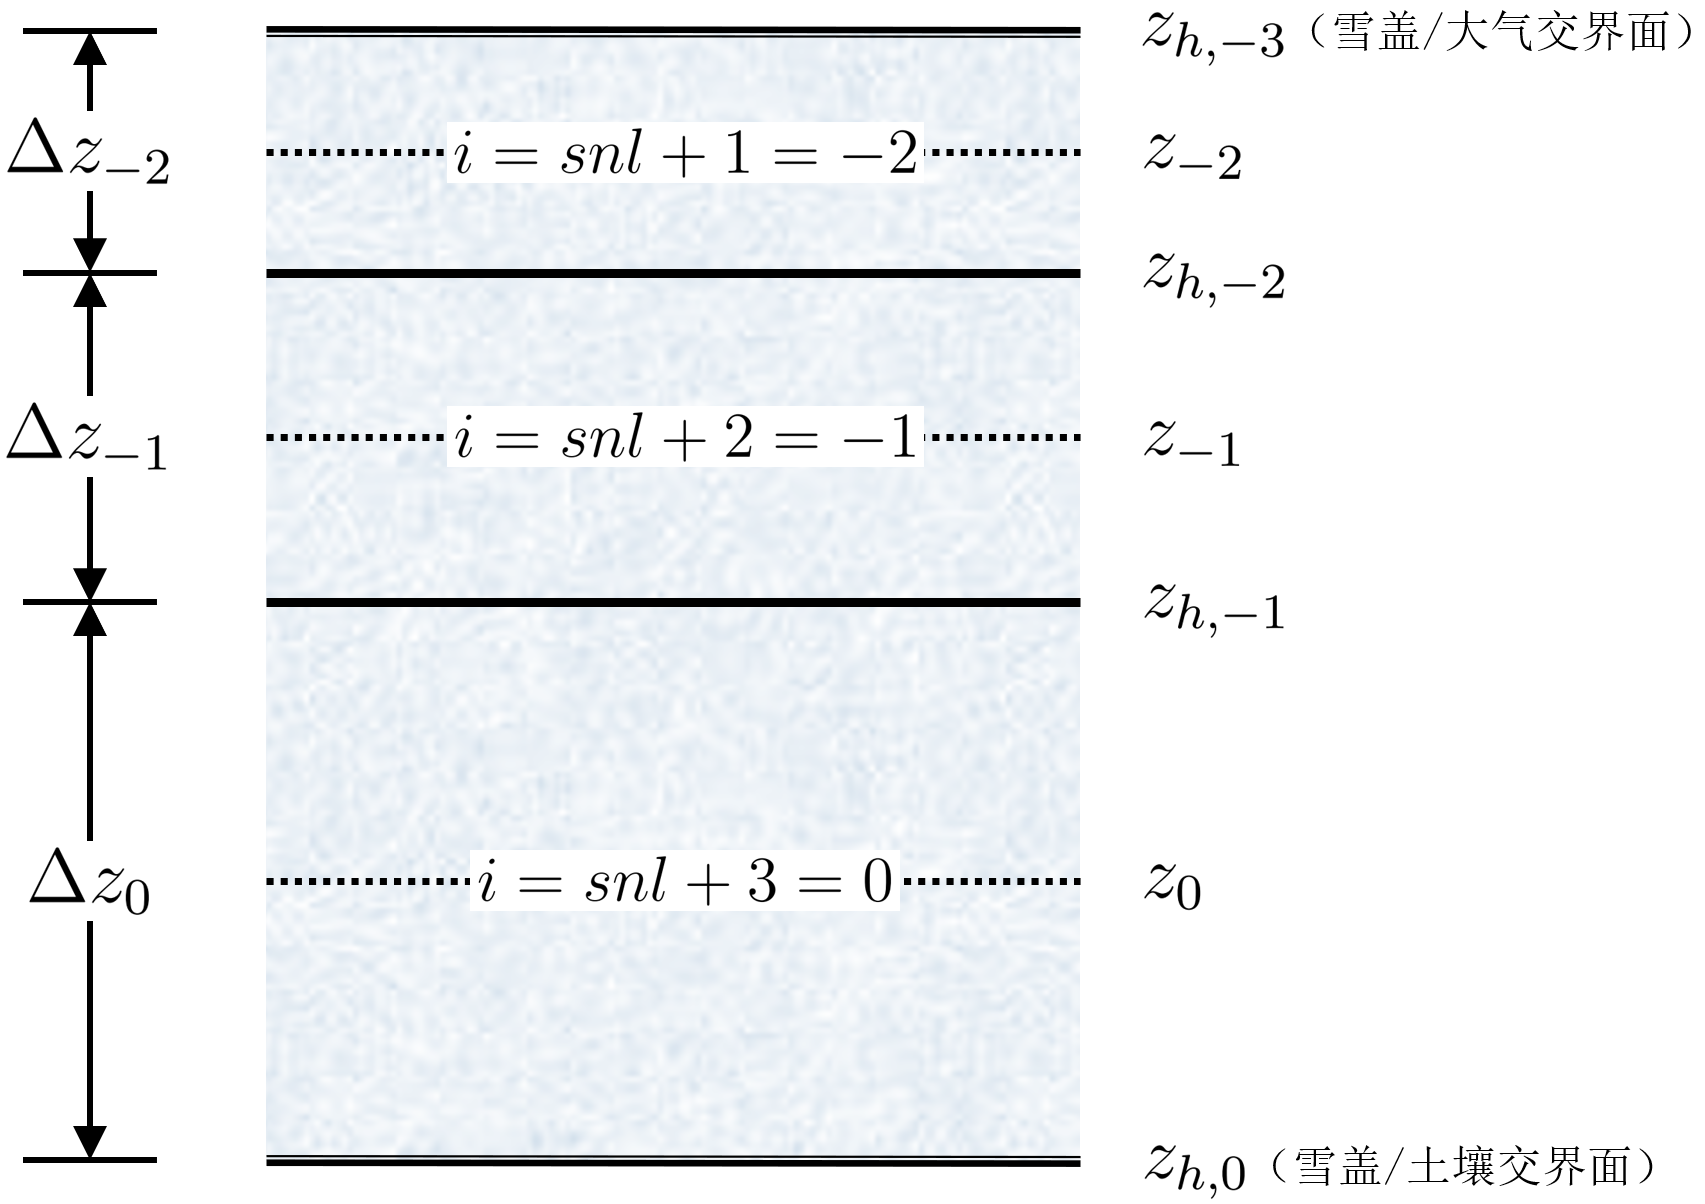
\includegraphics{Figures/雪盖土壤热力过程/模式中积雪雪层示意图.png}
\caption{模式中积雪雪层示意图(以三层雪层为例)。}
\label{fig:模式中积雪雪层示意图}
\end{figure}
}

当固态降水$q_{sno}$的发生导致总雪深 大于0.01 m时,若模式中没有已存在的雪层,则将在模拟开始时创建一个新的雪层,初始参数设置如下
\begin{equation}
\left\{\begin{array}{c}\Delta z_{0}={d}_{{sn}} \\ z_{0}=-0.5 \Delta z_{0} \\ z_{{h},-1}=-\Delta z_{0} \\ T_{0}=\min \left(T_{{f}}, T_{{atm}}\right) \\ {\left[{w}_{{ice}}\right]_{0}={W}_{{sno}}} \\ {\left[{w}_{\text {liq }}\right]_{0}=0}\end{array}\right.
\end{equation}
其中$T_f$为水的冻结温度,$T_{atm}$为大气温度,$w_{ice}$和$w_{liq}$分别表示雪层中冰的质量和液态水的质量(\unit{kg.m^{-2}})。


若模式中存在已建立的雪层,则固态降水产生的影响将添加至表层雪层,表层雪层因此而发生的改变如下:
\begin{equation}
\left\{\begin{array}{c}\Delta z_{[{snl}+1]^{*}}=\Delta z_{{snl}+1}+\Delta {d}_{{sn}} \\ {\left[z_{[{snl}+1]^{*}}\right]_{0}=-0.5 \Delta z_{[{snl}+1]^{*}}} \\ z_{{h}, {snl}^{*}}=z_{{h}, {snl}+1}-\Delta z_{[{snl}+1]^{*}} \\ {\left[{w}_{{ice}}\right]_{[{snl}+1]^{*}}=\Delta {W}_{{sno}}}\end{array}\right.
\end{equation}
其中$\ast$表示改变后的雪层。


\subsection{雪的压实}
\begin{mymdframed}{代码}
本节对应的代码文件为\texttt{MOD\_SnowLayersCombineDivide.F90}。
\end{mymdframed}
积雪压实的过程主要由以下四种变质作用造成:破坏(destructive)变质作用、压力(pressure)变质作用、结构(constructive)变质作用和融化(melt)变质作用 \citep{yen1981review}。在当前版本CoLM中,只实现了三种变质作用:破坏变质作用、负重(overburden)变质作用(或压力变质作用)和融化变质作用。前两种变质作用的处理方法来自 SNTHERM.89 \citep{jordan1991one}和 SNTHERM.99 \citep{jordan1999heat},融化变质作用的贡献简单地取为融化后与融化前的雪/冰比例。自然压实率的总分量可写成

\begin{equation}
{C}_{{R}}=\left[\frac{1}{\Delta {z}} \frac{\partial \Delta {z}}{\partial {t}}\right]_{\text {destructive }}+\left[\frac{1}{\Delta {z}} \frac{\partial \Delta {z}}{\partial {t}}\right]_{\text {overburden }}+\left[\frac{1}{\Delta {z}} \frac{\partial \Delta {z}}{\partial {t}}\right]_{\text{melt}}
\end{equation}
由于压实导致的雪层厚度为:
\begin{equation}
\Delta z_{j}=\Delta z_{j}^{\prime}\left(1+C_{R, j} \Delta t\right)
\end{equation}
其中$\Delta {z}_{{j}}^{\prime}$ 为未压实前第$j$层雪层的厚度。


\begin{enumerate}
\item 破坏变质下的积雪沉降\\
雪到达地面后,随即开始快速变化,单个雪花会迅速失去原有形状,变成更具球形。在风或热力的作用下,新雪的星形晶状结构破裂,雪堆发生沉降,雪粒堆积。对于密度小于 \qty{100}{kg.m^{-3}} 的新雪来说,破坏变质引起的沉降非常重要。新雪由于星形雪粒之间的“齿轮咬合”作用而具有一定的结构强度,这种结构在变质作用中会逐渐丧失。\citet{anderson1976point}对这一阶段的压实过程提出了以下经验函数:
\begin{equation}\label{eq:Delta_Z}
\left[\frac{1}{\Delta {z}} \frac{\partial \Delta {z}}{\partial {t}}\right]_{\text {destructive }}=-2.778 \times 10^{-6} {c}_{3} {c}_{4} {e}^{-0.04\left({~T}_{{f}}-{T}\right)}
\end{equation}
式中${c}_{3}={c}_{4}=1$
当雪层中冰的体积密度$\rho_{i} \theta_{i}>100$ \unit{kg.m^{-3}} 时
\begin{equation}
{C}_{3}={e}^{-0.046\left(\rho_{{i}} \theta_{{i}}-100\right)}, \quad {C}_{4}=1
\end{equation}
当雪层中液态水的体积密度$\rho_{1} \theta_{1}>0.01$ \unit{kg.m^{-3}} 时
\begin{equation}
{C}_{3}=1,\quad  {C}_{4}=2
\end{equation}
即根据式~\eqref{eq:Delta_Z} 预测的密度小于 \qty{100}{kg.m^{-3}} 的积雪,破坏变质导致的形变率为每小时 1\%,当雪层中冰的体积密度超过 \qty{100}{kg.m^{-3}} 时,破环变质的速率会有所降低,而当雪层中存在液态水时,破环变质的速率将为原来的两倍。

\item 雪层负重引起的压实\\
随着积雪的累积,上覆积雪的自重会进一步地压实雪层。上覆雪层产生的压力导致雪粒粘结生长速度加快,形成更加有效的堆积形状。在经过最初的沉降阶段后,这一阶段的压实速度会减慢,很大程度上取决于雪层负重带来的压力。在低压力范围的季节性积雪内,雪的形变率是压力的线性函数,即
\begin{equation}
\left[\frac{1}{\Delta {z}} \frac{\partial \Delta {z}}{\partial {t}}\right]_{\text {overburden }}=-\frac{{P}_{{s}}}{9 \times 10^{5}} {e}^{-0.08\left({~T}_{{f}}-{T}\right)-0.023 \rho_{{i}} \theta_{{i}}}
\end{equation}
其中$P_{s}$是上覆雪的重量(\unit{kg.m^{-2}}),对于第$j$层,其上覆雪的重量由以下公式得出
\begin{equation}
\left[P_{s}\right]_{j}=\frac{\left[w_{\text {ice }}\right]_{j}+\left[w_{\text {liq }}\right]_{j}}{2}+\sum_{{i}={snl}+1}^{{i}={j}-1}\left(\left[{w}_{{ice}}\right]_{{i}}+\left[{w}_{\text {liq }}\right]_{{i}}\right)
\end{equation}

\item 雪层融化引起的压实。\\
在融雪过程的后期(雪经过多次冻融循环后),融雪水的出流导致雪层压实,雪堆过度致密:
\begin{equation}
\left[\frac{1}{\Delta {z}} \frac{\partial \Delta {z}}{\partial {t}}\right]_{{melt}}=\frac{1}{\Delta {t}}\left[\frac{{f}_{{I}}^{{n}+1}-{f}_{{I}}^{{n}}}{{f}_{{I}}^{{n}}}\right]
\end{equation}
\end{enumerate}
\subsection{雪层的合并}
\begin{mymdframed}{代码}
本节对应的代码文件为\texttt{MOD\_SnowLayersCombineDivide.F90}。
\end{mymdframed}
当某一雪层完全融化或其厚度小于规定的最小值时,则将该雪层与邻近雪层合并。根据以下标准选择相邻的上层或下层雪层进行合并:
\begin{enumerate}
\item 如果为表面雪层,则将其与相邻的下层雪层合并;
\item 如果为与土壤相邻的底层雪层,则将其与相邻的上层雪层合并;
\item 如果为已完全融化的中间雪层,则将其与相邻的下层雪层合并;以及
\item 如果上述情况均不适用,则将该雪层与较薄的相邻雪层合并。
五个雪层(从表层到底层)的厚度最小值分别为 0.010、0.015、0.025、0.055 和 0.115(米)。

\end{enumerate}


\subsubsection{质量和能量再分配}

当两个雪层(用$j$和$j+1$表示)合并时,它们合并后的厚度为
\begin{equation}
\Delta {z}_{{j} *}=\Delta {z}_{{j}}+\Delta {z}_{{j}+1}
\end{equation}
合并后的质量为
\begin{equation}
\left[{w}_{{liq}}\right]_{{j}^{*}}=\left[{w}_{{liq}}\right]_{{j}}+\left[{w}_{{liq}}\right]_{{j}+1}
\end{equation}
\begin{equation}
\left[{w}_{ {ice }}\right]_{j *}=\left[{w}_{ {ice }}\right]_{j}+\left[{w}_{ {ice }}\right]_{j+1}
\end{equation}
合并后的温度根据焓的守恒,由以下公式得出
\begin{equation}
\begin{array}{l}h_{j}=\left[c_{i} w_{ {ice }}+c_{1} w_{ {liq }}\right]_{j} \times\left[T_{j}-T_{f}\right]+L_{f}\left[w_{ {liq }}\right]_{j} \\ h_{j+1}=\left[c_{i} w_{ {ice }}+c_{1} w_{ {liq }}\right]_{j+1} \times\left[T_{j+1}-T_{f}\right]+L_{f}\left[w_{ {liq }}\right]_{j+1} \\ h_{j *}=h_{j}+h_{j+1}\end{array}
\end{equation}
\begin{equation}
{T}_{{j}^{*}}=\left\{\begin{array}{ll}{T}_{{f}}+{h}_{{j}^{*}} /\left[{c}_{1} {w}_{\text {liq }}+{c}_{{i}} {w}_{{ice}}\right]_{{j}^{*}}, & \text { for } {h}_{{j}^{*}}<0 \\ {~T}_{{f}}, & \text { for } {h}_{{j}^{*}} \leq {L}_{{f}}\left[{w}_{{liq}}\right]_{{j}^{*}} \\ {~T}_{{f}}-\left({h}_{{j}^{*}}-{L}_{{f}}\left[{w}_{{liq}}\right]_{{j}^{*}}\right) /\left[{c}_{{l}} {w}_{{liq}}+{c}_{{i}} {w}_{{ice}}\right]_{{j}^{*}}, & \text { for } {h}_{{j}^{*}}>{L}_{{f}}\left[{w}_{{liq}}\right]_{{j}^{*}}\end{array}\right.
\end{equation}


\subsubsection{气溶胶通量的计算}

本版本CoLM在计算雪层的合并与细分时,添加了SNICAR模型可供选择。当使用SNICAR模型时,会额外计算雪层合并后的黑碳、有机碳和矿物粉尘的质量,均采用以下公式得出
\begin{equation}
\left[m_{\mathrm{sp}}\right]_{j^{*}}=\left[m_{\mathrm{sp}}\right]_{j}+\left[m_{\mathrm{sp}}\right]_{j+1}
\end{equation}
其中下标sp可表示不同的黑碳、有机碳和粉尘种类。
\subsubsection{雪层的细分}
当某一雪层的厚度超过规定的最大厚度(从表层到底层分别为,0.02、0.05、0.11、0.23 和 > 0.23 米)时,雪层将被细分。如果被细分的雪层没有已存在的相邻下层雪层,则该雪层被等分为厚度相同的两层,并具有同样的液态水含量、冰含量和温度。如果被细分的雪层有相邻的下层雪层,则将多余的雪层厚度、液态水含量、冰含量以及温度属性和下层雪层合并。细分规则如图~\ref{fig:情况1-5} 和~\ref{fig:情况6-9} 所示,图中$d_{sn}$为总雪深(米)。

{
\begin{figure}[]
\centering
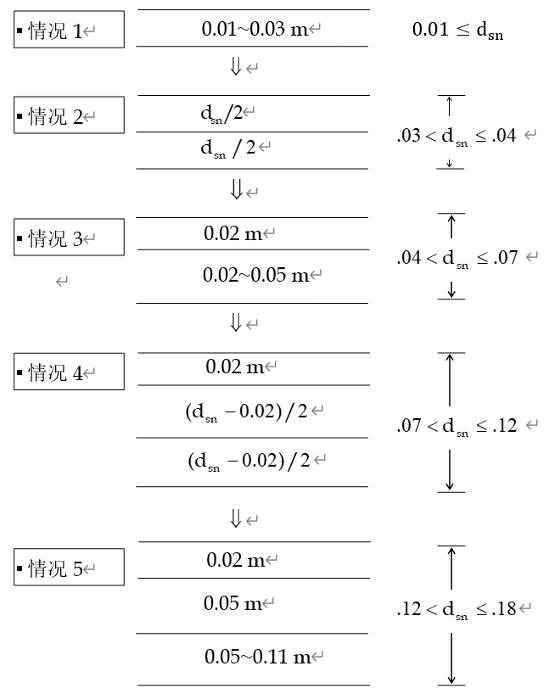
\includegraphics{Figures/雪盖土壤热力过程/情况1-5.png}
\caption{不同积雪高度下雪层厚度的分层规则。}
\label{fig:情况1-5}
\end{figure}
}

{
\begin{figure}[]
\centering
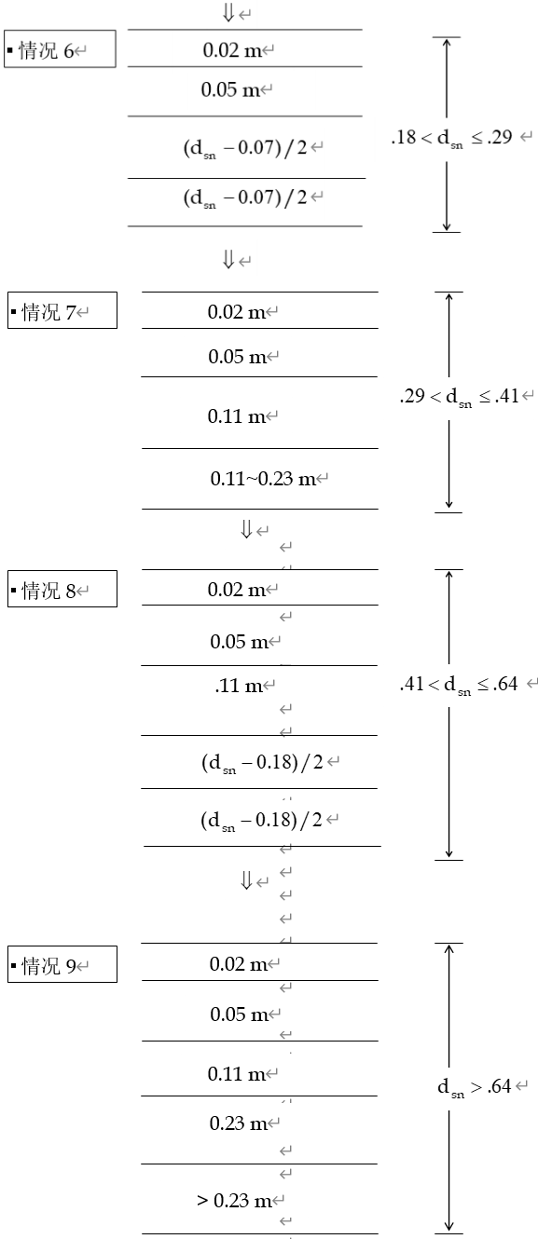
\includegraphics{Figures/雪盖土壤热力过程/情况6-9.png}
\caption{不同积雪高度下雪层厚度的分层规则续}
\label{fig:情况6-9}
\end{figure}
}

\chapter{陆地表面的水分循环}
%\addcontentsline{toc}{chapter}{陆地表面的水分循环}

%\begin{陆地表面的水分循环}
陆地表面的水分循环过程为:
\begin{enumerate}
    \item 降水以液态(雨)或固态(雪)降落到地表,除去被植被截留的部分,其余降落到土壤表面,形成积雪或地面液态水;
    \item 地表液态水可积存在地面,可通过径流方式流走,可入渗到土壤中,或通过蒸发的方式返回大气中;若地表有积雪,积雪中的液态水会由于重力作用自上而下流到土壤表面;
    \item 土壤中的水分会在重力和毛细管力的作用下在土壤孔隙中流动;
    \item 受地势的影响,土壤中的水分会转化为地下径流流走。
\end{enumerate}

对于土壤表面的水分输入,若土壤表面无积雪,则土壤表面水分的输入为
\begin{equation}
G_{water}=P_{ground}+S_{melt}-E
\end{equation}
其中$G_{water}$为到达土壤表面的净水分输入,$P_{ground}$为经植被截留后到达地面的降水,$S_{melt}$为融化的雪水,$E$为土壤表面的蒸发。

若土壤表面有积雪,则考虑水分自上而下到达土壤表面的过程。对最上层积雪,冰的变化量为结霜的量减去升华的量;液态水的增加来自到达雪表面的降水和气态水的凝结,减少的量为蒸发。

积雪中的液态水受毛细管力和重力的共同作用而流动,但由于毛细管力比重力小两个以上数量级,在计算的时候可以忽略。
水流通量一般表达为$K\times{\rm ss}^3$,其中$K$为导水率,$ss$为液态水在孔隙中的饱和度。由于没有有效的参数化方案来计算导水率$K$,
模式中采用简化的方案来近似液态水在积雪中的流动:当某一层中的液态水的含量超过了这一层的持水能力的时候,多余的液态水自这一层流入其下的一层。
最下层的液态水运动,形成对土壤的入渗或地表径流。下面依次从植被到土壤分别介绍各水文循环过程的描述。
\section{植被冠层截留}\label{植被冠层截留}
CoLM冠层水库的水平衡方程基本与SiB2一致 \citet{sellers1996revised},主要基于以下控制方程:
\begin{equation}
\partial M_{c w, s}=P-D_{d}-D_{c}-E_{c i} / \rho_{w}
\end{equation}
式中 $P$ 为总降水量($\rm m s^{-1}$),分为对流降水和大尺度降水类型:
\begin{equation}
P=P_{c}+P_{l}=\left(R_{c}+S_{c}\right)+\left(R_{l}+S_{l s}\right)
\end{equation}
其中下标$c$和$l$代表对流和大尺度降水类型,$R$和$S$分别代表降雨率与降雪率 (($\rm m s^{-1}$)。
当驱动强迫场中只有总降水可用时,CoLM假设大尺度降水等于$1/3P$,对流降水占$2/3P$。
$D_d$为降雨穿透速率 ($\rm m s^{-1}$),即从冠层间隙下落的降水速率,$D_c$为冠层排水速度 ($\rm m s^{-1}$),$\partial M_{cw,s}$为冠层蓄水变化率 ($\rm m s^{-1}$), 
$\rho_w$是水的密度, $E_{ci}$为蒸发速率。此处的直接穿透量$D_d$与辐射传输中的光穿透量的计算方法一致,由下式给出:
\begin{equation}
D_{d}=\delta_{P} \cdot P=\delta_{P} \cdot\left(R_{c}+S_{c}+R_{l}+S_{l s}\right)
\end{equation}
其中$\delta_P$是冠层穿透系数, 等于
\begin{equation}
\delta_{P}=1.0-\alpha \times\left[1-\exp \left(-K_{p} \times LSAI\right)\right]
\end{equation}
该公式中反映叶片集水能力的经验系数$\alpha$被设定为0.25 \citep{lawrence2011parameterization}。
$LSAI$是$SAI$和$LAI$之和 ($LAI$和$SAI$分别是叶指数和茎面积指数);$K_p$是消光系数,与辐射在冠层中的穿透计算相同:
\begin{equation}
\begin{array}{c}K_{p}=\phi_{1}+\phi_{2} \\ \phi_{2}=0.877\left(1-2 \phi_{1}\right) \\ \phi_{1}=0.5-0.633 \chi_{L}-0.33 \chi_{L}^{2}\end{array}
\end{equation}
$K_p$通过叶角分布的经验参数$\chi_L$的变化来控制,
其中$\chi_L=0$表示球形叶角分布,$\chi_L= 1$ 表示水平方向的叶子,$\chi_L= -1$ 表示垂直方向的叶子。
根据植被类型,$\chi_L$的范围在-0.3$\sim$0.25之间。由此计算得出的$\delta_P$的变动范围如图 \ref{fig:穿透系数与叶面积指数} 所示:
{
\begin{figure}[]
\centering
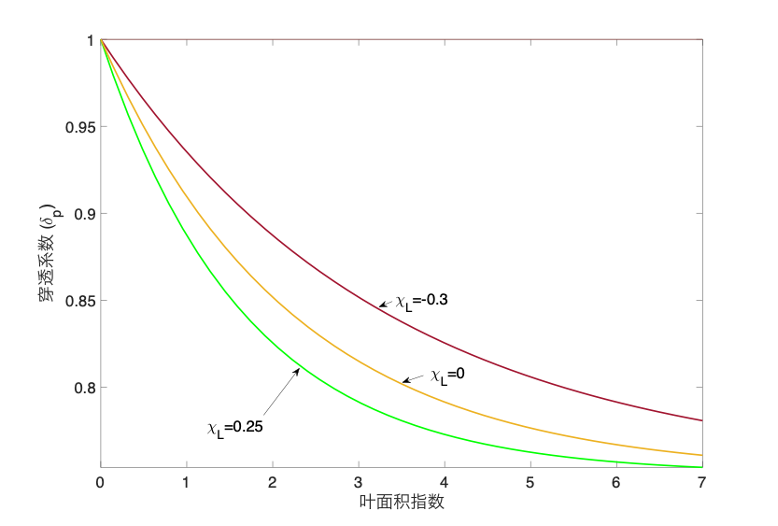
\includegraphics{Figures/陆地表面的水分循环/穿透系数与叶面积指数.png}
\caption{穿透系数$\delta_P$与叶面积指数的关系及其变动范围。}
\label{fig:穿透系数与叶面积指数}
\end{figure}
}
为防止升华或冷凝水超过最大树冠储存量,CoLM在计算冠层截留之前首先更新树叶上的水深 ($Ldew$) (mm):
\begin{equation}
\begin{array}{c}L_{d e w}=L_{d e w}-x_{s c} \\ x_{s c}=\max \left(0 ., L_{d e w}-x_{s c}\right)\end{array}
\end{equation}
其中xsc是超过最大树冠储存量的水(mm),$S_c=0.1f_{sig}\left(LAI+SAI\right)$代表最大蓄水量(mm)。
$xsc$的相位首先由冠层温度决定。如果冠层温度大于冰点温度,CoLM假定所有过量的水都处于液相,否则处于冰雪相。


CoLM 假设网格内的降水的分布是不均匀的。其中对流降水面积的网格占比$I_c$可以由下式给出
\begin{equation}
I_{c}(x)=a_{c} e^{-b x}+c_{c}
\end{equation}
其中$a_c=20$,$b=20$ 和 $c_c=0.206\times10^{-8}$是常数。大尺度降水面积的网格占比$I_l$可以用相同的形式表示:
\begin{equation}
I_{l}(x)=a_{l} e^{-b x}+c_{l}
\end{equation}
其中$a_l=0.0001$和$c_l=0.9999$。因此,通过组合这两个方程给出了有效降雨占比区域的降雨强度为:
\begin{equation}
P I(x)=\left(a_{l} P_{l}+a_{c} P_{c}\right) e^{-b x}+\left(c_{l} P_{l}+c_{c} P_{c}\right)
\end{equation}
因此,有效降雨区域的树冠排水由下式给出:
\begin{equation}
t h r u_{ {rain }}=\int_{0}^{x_{s}} P I(x) d x+L_{d e w} x_{s}-S_{c} x_{s}
\end{equation}
其中$x_s$是单位网格中“截获降雨加上原有冠层蓄水量超过冠层上允许的最大水深($S_c$)”的比例:
\begin{equation}
x_{s}=\frac{-1}{b} \log \left[\frac{s_{c}-L_{d e w}}{a_{p}\left(P-D_{d}\right)}-\frac{c_{p}}{a_{p}}\right]
\end{equation}
其中$a_p=\frac{a_lP_l+a_cP_c}{P}$,$c_p=\frac{c_lP_l+c_cP_c}{P}$。这里假设只有液态水能够被冠层所截获,我们有
\begin{equation}
t h r u_{ {rain }}=\left(R_{c}+R_{l}\right)\left(1-\delta_{p}\right) \frac{a_{p}}{b}\left(1-e^{-b x_{s}}\right)+c_{p} x_{s}+L_{d e w} x_{s}-S_{c} x_{s}
\end{equation}
在整体网格尺度上$D_c$被更新为
\begin{equation}
D_c=thru_{r a i n}+x_{s c}
\end{equation}
因此,保留在树冠上的可用于树冠蒸发(截留蒸发)的蓄水量$I$(mm)可以由下式进行更新:
\begin{equation}
I={P}-D_{c}-D_{d}
\end{equation}
在冠层蒸发量的计算上首先需要计算湿叶茎面积占总叶茎面积的比例 ($f_{wet}$)。该计算CoLM模型采用\citet{dickinson1993biosphere}提出的经验方法
\begin{equation}
f_{{wet}}=\left(\frac{L_{d e w}}{s_{c}}\right)^{2 / 3} \leq 1.0
\end{equation}
其中$L_{dew_p}$是上一步计算得出的可用于树冠蒸发的蓄水量 (m);网格中有效植被的比例为$f_{sig}=\left(1-wt\right)f_{evg}$。
$f_{evg}$是任意网格中植被的比例,$wt$是被雪掩埋的植被占总植被的比例,由下式给出:
\begin{equation}
w t=\frac{0.1 Z_{sno}}{z_{vm}+0.1 Z_{sno}}
\end{equation}
其中$Z_{sno}$代表积雪厚度 (m),$Z_{vm}$代表植被粗糙度 (m)。因此,树冠蒸发量计算如下:
\begin{equation}
E_{ci} / \rho_{w}=\min \left(\frac{\left(q_{s}-q_{sat}^{T_{c}}\right)}{r_{b} /\left(LSAI \times f_{wet}\right)}, \frac{L_{dew_{d} t}}{\Delta t}\right)
\end{equation}
这里$r_b$是平均边界层阻力,由冠层顶部的风速和特征叶片尺寸确定;$q_{sat}^{T_c} $(kg/kg)是冠层温度下的饱和比湿度;$q_s$为表层参考高度处的比湿度,$\Delta t$为时间步长。


\section{地表径流}
地表径流的参数化方案考虑了地形、地下水位、降水和入渗速度等因素。
模式网格内饱和区域的面积$f_{sat}$通过以下方案估算,
\begin{equation}
f_{sat}=f_{w t} \times e^{-0.5 \times fff \times z_{wt}}
\end{equation}
其中,$f_{wt}$为网格内地下水位较高的区域的面积百分比,$fff$为径流的衰减因子,$z_{wt}$为地下水位的位置。

最大入渗能力的计算考虑了最上面三层土壤的物理状态和属性,
\begin{equation}
q_{i n, \max }=\min _{i=1,2,3} 10^{-6.0 \times f_{i c e, i} \times K_{sat, i}}
\end{equation}
其中,$f_{ice,i}$表示第i层中冰占土壤孔隙的体积百分比,$K_{sat,i}$表示第$i$层的饱和导水率。

一个模式网格内,饱和区域的地表水全部转化为径流流走,非饱和区域的地表水,部分入渗到土壤中,剩余部分转化为径流,总的地表径流为:
\begin{equation}
\r_{surface }=f_{sat} \times G_{water}+\left(1-f_{sat}\right) \times \left(G_{water}-q_{inmax}\right)
\end{equation}
入渗到土壤中的部分等于表面水分的输入减去地表径流,即
\begin{equation}
q_{infl}={G}_{water}-r_{surface}
\end{equation}


\section{土壤水的运动}\label{sec:土壤水的运动}
土壤水的状态和垂直运动主要取决于地表入渗、地下径流、土水势的梯度、重力和植被根部对水的吸收等过程。模式中仅考虑土壤水在垂直方向上的运动。


在非饱和区域,土壤水通量用Buckingham-Darcy定律来描述,
\begin{equation}
q=-K \frac{\partial}{\partial z}(\psi-z)
\end{equation}
其中,$z$为土壤深度,取土壤表面为0,垂直向下为正方向,$\psi$为土壤水势,$K$为土壤导水率。


土壤导水率$K$和土水势$\psi$与土壤含水量和土壤质地有关,基于 \citet{clapp1978empirical} 和 \citet{cosby1984statistical} 的工作,
\begin{equation}
\psi=\psi_{s}\left(\frac{\theta}{\theta_{sat}}\right)^{-B}
\end{equation}
\begin{equation}
K=K_{sat}\left(\frac{\theta}{\theta_{sat}}\right)^{2 B+3}
\end{equation}
其中$\psi_s$为饱和土水势,$\theta_{sat}$为饱和土壤体积含水量,$K_{sat}$为饱和导水率,
$\theta$为土壤体积含水量,参数$\psi_s$,$\theta_{sat}$,$K_{sat}$,$B$均依赖于土壤质地。


根据质量守恒定律,可得一维土壤水的垂直运动方程(Richards方程),
\begin{equation}
\frac{\partial \theta}{\partial t}=-\frac{\partial q}{\partial z}-Q
\end{equation}
其中$Q$为土壤水的汇,主要为由于根系吸水作用(蒸腾)而减少的水分。


为求解Richards方程,需将土壤在垂直方向分层,
分层方案与计算土壤温度时采用的方案相同。在第$i$层上,对Richards方程进行空间上的积分可得
\begin{equation}
\Delta z_{i} \frac{\partial}{\partial t} \theta_{i}=-\left(q_{i+\frac{1}{2}}-q_{i-\frac{1}{2}}\right)-e_{i}
\end{equation}
\begin{equation}
q_{i+1 / 2}=-K_{i+1 / 2}\left(\frac{\psi_{i+1}-\psi_{i}}{\Delta z_{i}}-1\right)
\end{equation}
其中$\Delta {z_i}$为第$i$层的厚度,$\theta_i$为第$i$层的平均土壤含水量,
$q_{i+\frac{1}{2}}$为第$i$层和第$i+1$层之间的土壤水通量,$q_{i-\frac{1}{2}}$为第$i-1$层和第$i$层之间的土壤水通量,
$e_i$为第$i$层被根系吸收的水分。在时间上采用隐格式,可得
\begin{equation}
\Delta z_{i} \frac{\theta_{i}^{n+1}-\theta_{i}^{n}}{\Delta t}=-\left(q_{i+\frac{1}{2}}^{n+1}-q_{i-\frac{1}{2}}^{n+1}\right)-e_{i}
\end{equation}
\begin{equation}
q_{i+\frac{1}{2}}^{n+1}=-K_{i+\frac{1}{2}}^{n+1}\left(\frac{\psi_{i+1}^{n+1}-\psi_{i}^{n+1}}{\Delta z_{i, i+1}}-1\right)
\end{equation}
其中$\Delta z_{i,i+1}$表示从第i层到第$i+1$层中心的距离。
为了简化计算,将$q_{i+\frac{1}{2}}^{n+1}$表达式中的各项在$\theta_i^n$附近做一阶近似,可得
\begin{equation}
\begin{array}{c}K_{i+\frac{1}{2}}^{n+1}=K_{i+\frac{1}{2}}^{n}+\frac{\partial K_{i+\frac{1}{2}}}
    {\partial \theta_{i}}\left(\theta_{i}^{n+1}-\theta_{i}^{n}\right)+\frac{\partial K_{i+\frac{1}{2}}}
    {\partial \theta_{i+1}}\left(\theta_{i+1}^{n+1}-\theta_{i+1}^{n}\right) \\ 
    \psi_{i+1}^{n+1}=\psi_{i+1}^{n}+\frac{\partial \psi_{i+1}}{\partial \theta_{i+1}}\left(\theta_{i+1}^{n+1}-\theta_{i+1}^{n}\right)
     \\ \psi_{i}^{n+1}=\psi_{i}^{n}+\frac{\partial \psi_{i}}{\partial \theta_{i}}\left(\theta_{i}^{n+1}-\theta_{i}^{n}\right)\end{array}
\end{equation}
记$\Delta \theta_i=\theta_i^{n+1}-\theta_i^n$,则
\begin{equation}
\begin{split} 
q_{i+\frac{1}{2}}^{n+1} =&-\left(K_{i+\frac{1}{2}}^{n}+\frac{\partial K_{i+\frac{1}{2}}}{\partial \theta_{i}} \Delta \theta_{i} + \frac{\partial K_{i+\frac{1}{2}}}{\partial \theta_{i+1}} \Delta \theta_{i+1}\right)  \\
    & \times \left(\frac{1}{\Delta z_{i, i+1}}\left(\psi_{i+1}^{n}+\frac{\partial \psi_{i+1}}{\partial \theta_{i+1}} \Delta \theta_{i+1}-\psi_{i}^{n}-\frac{\partial \psi_{i}}
    {\partial \theta_{i}} \Delta \theta_{i}\right)-1\right) \\ 
    \approx & -K_{i+\frac{1}{2}}^{n}\left(\frac{1}{\Delta z_{i, i+1}}\left(\psi_{i+1}^{n}-\psi_{i}^{n}\right)-1\right) \\
    &-\left(-\left(K_{i+\frac{1}{2}}^{n} \frac{1}{\Delta z_{i, i+1}} \frac{\partial \psi_{i}}{\partial \theta_{i}}\right)+\frac{\partial K_{i+\frac{1}{2}}}{\partial 
     \theta_{i}}\left(\frac{1}{\Delta z_{i, i+1}}\left(\psi_{i+1}^{n}-\psi_{i}^{n}\right)-1\right)\right) \Delta \theta_{i} \\ 
    &-\left(\left(K_{i+\frac{1}{2}}^{n} \frac{1}{\Delta z_{i, i+1}} \frac{\partial \psi_{i+1}}{\partial \theta_{i+1}}\right)+\frac{\partial K_{i+\frac{1}{2}}}{\partial
      \theta_{i+1}}\left(\frac{1}{\Delta z_{i, i+1}}\left(\psi_{i+1}^{n}-\psi_{i}^{n}\right)-1\right)\right) \Delta \theta_{i+1} 
\end{split}
\end{equation}
对$q_{i-\frac{1}{2}}^{n+1}$也可做同样的近似。从而,完全离散后的Richards方程可表达为,
\begin{equation}
{a}_{{mx}} \Delta \theta_{i-1}+b_{m x} \Delta \theta_{i}+c_{m x} \Delta \theta_{i+1}=r_{m x}
\end{equation}
其中,
\begin{equation}
\begin{array}{c}{a}_{{mx}}=-\left(K_{i-\frac{1}{2}}^{n} \frac{1}{\Delta z_{i-1, i}}
     \frac{\partial \psi_{i-1}}{\partial \theta_{i-1}}\right)+\frac{\partial K_{i-\frac{1}{2}}}
     {\partial \theta_{i-1}}\left(\frac{1}{\Delta z_{i-1, i}}\left(\psi_{i}^{n}-\psi_{i-1}^{n}\right)-1\right) \\
      {b}_{{mx}}=\frac{\Delta z_{i}}{\Delta t}-\left(-\left(K_{i+\frac{1}{2}}^{n} \frac{1}{\Delta z_{i, i+1}} 
      \frac{\partial \psi_{i}}{\partial \theta_{i}}\right)+\frac{\partial K_{i+\frac{1}{2}}}{\partial \theta_{i}}
      \left(\frac{1}{\Delta z_{i, i+1}}\left(\psi_{i+1}^{n}-\psi_{i}^{n}\right)-1\right)\right) \\
       +\left(\left(K_{i-\frac{1}{2}}^{n} \frac{1}{\Delta z_{i-1, i}} \frac{\partial \psi_{i}}{\partial 
       \theta_{i}}\right)+\frac{\partial K_{i-\frac{1}{2}}}{\partial \theta_{i}}\left(\frac{1}{\Delta z_{i-1, i}}\left(\psi_{i}^{n}
       -\psi_{i-1}^{n}\right)-1\right)\right) \\ {c}_{{mx}}=-\left(\left(K_{i+\frac{1}{2}}^{n} \frac{1}{\Delta z_{i, i+1}} 
       \frac{\partial \psi_{i+1}}{\partial \theta_{i+1}}\right)+\frac{\partial K_{i+\frac{1}{2}}}{\partial \theta_{i+1}}\left(\frac{1}
       {\Delta z_{i, i+1}}\left(\psi_{i+1}^{n}-\psi_{i}^{n}\right)-1\right)\right) \\ r_{m x}=K_{i+\frac{1}{2}}^{n}
       \left(\frac{1}{\Delta z}\left(\psi_{i+1}^{n}-\psi_{i}^{n}\right)+1\right)-K_{i-\frac{1}{2}}^{n}
       \left(\frac{1}{\Delta z}\left(\psi_{i}^{n}-\psi_{i-1}^{n}\right)-1\right)-e_{i}\end{array}
\end{equation}
对最上面的土壤分层(第1层),使用给定的入渗通量$q_{infl}$,则
\begin{equation}
\begin{array}{c}{a}_{{mx}}=0 \\ {~b}_{{mx}}=\frac{\Delta z_{i}}{\Delta t}-\left(-\left(K_{i+\frac{1}{2}}^{n} 
    \frac{1}{\Delta z_{i, i+1}} \frac{\partial \psi_{i}}{\partial \theta_{i}}\right)+\frac{\partial K_{i+\frac{1}{2}}}{\partial \theta_{i}}\left(\frac{1}{\Delta z_{i, i+1}}
    \left(\psi_{i+1}^{n}-\psi_{i}^{n}\right)-1\right)\right) \\ {c}_{{mx}}=-\left(\left(K_{i+\frac{1}{2}}^{n} \frac{1}{\Delta z_{i, i+1}} 
    \frac{\partial \psi_{i+1}}{\partial \theta_{i+1}}\right)+\frac{\partial K_{i+\frac{1}{2}}}{\partial \theta_{i+1}}\left(\frac{1}{\Delta z_{i, i+1}}
    \left(\psi_{i+1}^{n}-\psi_{i}^{n}\right)-1\right)\right) \\ r_{m x}=q_{i n f l}+K_{i+\frac{1}{2}}^{n}
    \left(\frac{1}{\Delta z}\left(\psi_{i+1}^{n}-\psi_{i}^{n}\right)-1\right)-e_{i}\end{array}
\end{equation}
对最下面的土壤分层,假定边界条件为重力排水边界条件,即$q_{i+\frac{1}{2}}^{n+1}=-K_{i+\frac{1}{2}}^{n+1}$,则
\begin{equation}
\begin{array}{c}{a}_{{mx}}=-\left(K_{i-\frac{1}{2}}^{n} \frac{1}{\Delta z_{i-1, i}} \frac{\partial \psi_{i-1}}
    {\partial \theta_{i-1}}\right)+\frac{\partial K_{i-\frac{1}{2}}}{\partial \theta_{i-1}}\left(\frac{1}{\Delta z_{i-1, i}}
    \left(\psi_{i}^{n}-\psi_{i-1}^{n}\right)-1\right) \\ {b}_{{mx}}=\frac{\Delta z_{i}}{\Delta t}+\frac{\partial K_{i+\frac{1}{2}}}
    {\partial \theta_{i}}+\left(\left(K_{i-\frac{1}{2}}^{n} \frac{1}{\Delta z_{i-1, i}} \frac{\partial \psi_{i}}{\partial \theta_{i}}\right)+
    \frac{\partial K_{i-\frac{1}{2}}}{\partial \theta_{i}}\left(\frac{1}{\Delta z_{i-1, i}}\left(\psi_{i}^{n}-\psi_{i-1}^{n}\right)-1\right)\right) \\
     c_{{mx}}=0 \\ r_{m x}=-K_{i+\frac{1}{2}}^{n}-K_{i-\frac{1}{2}}^{n}\left(\frac{1}{\Delta z}\left(\psi_{i}^{n}-\psi_{i-1}^{n}\right)-1\right)-e_{i}\end{array}
\end{equation}
求解上述方程组,即可得到土壤水含量的变化量。方程组的系数矩阵为三对角阵,可用追赶法快速求解。


在系数矩阵中,需要对土水势和导水率函数求导数。对土水势,容易计算得到
\begin{equation}
\frac{\partial \psi_{i}}{\partial \theta_{i}}=-B \frac{\psi_{i}}{\theta_{i}}
\end{equation}
对导水率,若采用迎风格式
\begin{equation}
    K_{i+1/2}=\left\{\begin{array}{l}K_{ {sat }}\left(\frac{\theta_{i}}{\theta_{ {sat }}}\right)^{2 B+3},
        -\left(\frac{\psi_{i+1}-\psi_{i}}{\Delta z}-1\right) \geq 0 \\ K_{ {sat }}\left(\frac{\theta_{i+1}}{\theta_{ {sat }}}\right)^{2 B+3},
        -\left(\frac{\psi_{i+1}-\psi_{i}}{\Delta z}-1\right)<0\end{array}\right.
\end{equation}
则导数为
\begin{equation}
\frac{\partial K_{i+\frac{1}{2}}}{\partial \theta_{i}}=\left\{\begin{aligned}(2 B+3) K_{ {sat }}\left(\frac{\theta_{i}}{\theta_{sat}}\right)^{2 B+2} 
    \frac{1}{\theta_{s a}},-\left(\frac{\psi_{i+1}-\psi_{i}}{\Delta z}-1\right) & \geq 0 \\ 0,-\left(\frac{\psi_{i+1}-\psi_{i}}{\Delta z}-1\right) &<0 \end{aligned}\right.
\end{equation}
\begin{equation}
\frac{\partial K_{i+\frac{1}{2}}}{\partial \theta_{i+1}}=\left\{\begin{aligned} 0,-\left(\frac{\psi_{i+1}-\psi_{i}}{\Delta z}-1\right) &
     \geq 0 \\(2 B+3) K_{ {sat }}\left(\frac{\theta_{i+1}}{\theta_{ {sat }}}\right)^{2 B+2} \frac{1}{\theta_{ {sat }}},-\left(\frac{\psi_{i+1}-\psi_{i}}{\Delta z}-1\right) &<0 \end{aligned}\right.
\end{equation}
对计算区域的底部,
\begin{equation}
K_{i+1 / 2}=K_{ {sat }}\left(\frac{\theta_{i}}{\theta_{ {sat }}}\right)^{2 B+3}, \quad \frac{\partial K_{i+\frac{1}{2}}}
{\partial \theta_{i}}=(2 B+3) K_{ {sat }}\left(\frac{\theta_{i}}{\theta_{ {sat }}}\right)^{2 B+2} \frac{1}{\theta_{sat}}
\end{equation}
有冰存在的时候,需考虑冰对导水率的影响,使用如下经验公式,
\begin{equation}
    {f}_{{imped}, {i}+1 / 2}=10^{-e_{ice}\times 0.5\times\left(f_{i c e, i}+f_{i c e, i+1}\right)}
\end{equation}
其中$e_{ice}=6.0$为冰的阻抗因子。对导水率及其导数的调整为
\begin{equation}
\begin{array}{c}K_{i+\frac{1}{2}}={f}_{ {imped,i+ }+\frac{1}{2}} \times K_{i+\frac{1}{2}} \\ \frac{\partial K_{i+\frac{1}{2}}}{\partial \theta_{i}}
    ={f}_{ {imped,i+ }+\frac{1}{2}} \times \frac{\partial K_{i+\frac{1}{2}}}{\partial \theta_{i}} \\ \frac{\partial K_{i+\frac{1}{2}}}{\partial \theta_{i+1}}=
    {f}_{ {imped,i+ } \frac{1}{2}} \times \frac{\partial K_{i+\frac{1}{2}}}{\partial \theta_{i+1}}\end{array}
\end{equation}


对地下水的补给率定义为最下层土壤流出的水流通量,
\begin{equation}
{q}_{ {charge }}=q_{I+\frac{1}{2}}^{n+1}=K_{I+\frac{1}{2}}^{n}+\frac{\partial K_{I+\frac{1}{2}}}{\partial \theta_{I}} \Delta \theta_{I}
\end{equation}


这里对土壤水方程中的源汇项$Q$的主要来源,即根系吸水作用(蒸腾)过程做一简单介绍。植物吸水作用由有效根比例$f_{root,i}$和叶面蒸腾$Etr$的乘积来表示\citep{dai2003common}。有效根比例为:
\begin{equation}
{f}_{ {root }, {i}}=\frac{{f}_{{root}, {i}} {W}_{{LT}}[{i}]}{W_{t}}
\end{equation}
其中$Wt = \sum_{i=1}^{n}{f_{root,i\ }W_{LT}\left[i\right]}$;$f_{root,i}$表示模式中第$i$层土壤中的根系比例;$WLT[i]$表示第$i$层土壤中的水分胁迫状况:
\begin{equation}
{W}_{{LT}}[{i}]=\frac{\psi_{\max }-\psi_{i}}{\psi_{\max }-\psi_{sat}}
\end{equation}
其中,$\psi_{max}$为植物叶片干枯前的最大水势。


叶面蒸腾表示为:
\begin{equation}
{E}_{{tr}}=\sigma_{{f}} LSAI \delta\left({E}_{{f}}^{{pot}}\right) {L}_{{d}} \frac{{r}_{{b}}}{{r}_{{b}}-{r}_{{s}}} {E}_{{f}}^{{pot}} \leq {E}_{{trmax}}
\end{equation}
其中,$\sigma_f$表示没有被雪覆盖的植物比例,$LSAI$表示叶面积指数和茎面积指数之和,$\delta\left(E_f^{pot}\right)$为表示蒸发是否发生的参数,
取值0或1,$L_d$为干燥的植物表面比例,$r_b$为叶片边界层阻抗,$r_s$为叶片气孔阻抗。$E_f^{pot}$表示植物表面水的单位面积蒸发量:
\begin{equation}
{E}_{{f}}^{{pot}}=\rho_{{a}} {r}_{{b}}^{-1}\left({q}_{{f}}^{{sat}}-{q}_{{af}}\right)
\end{equation}
其中,$\rho_a$表示空气密度,$q_f^{sat}$表示冠层空气饱和比湿,$q_{af}$表示冠层空气比湿。$E_{trmax}$为最大蒸腾速率:
\begin{equation}
{E}_{ {trmax }}=2 \times 10^{-4} \times \sigma_{{f}} L A I \times W_{t}
\end{equation}
\section{地下水与土壤水的相互作用}
地下水的运动包含土壤水对地下水的补给和由地形起伏引起的地下径流。


给水度(specific yield)反映了地下水位变化时土壤水的变化量。模式中采用分析公式来计算,
\begin{equation}
{S}_{{y}}=\theta_{s}\left(1-\left(1-\frac{z_{w t}}{\psi_{s}}\right)^{-1 / b}\right)
\end{equation}
含水层水量的变化为
\begin{equation}
w_{a}=w_{a}+q_{charge} \times \Delta t
\end{equation}
若地下水位位于最下层土壤之下,则水位的变化为
\begin{equation}
Z_{w t}=z_{w t}-\frac{q_{charge} \times \Delta t}{s_{y}}
\end{equation}
若地下水位位于分层土壤之内,则需要逐层计算水位的变化。当$q_charge>0$时,
由地下水位所在一层开始,至最上层或补给水用尽结束,依次计算,
\begin{equation}
\begin{array}{c}{S}_{{y}}=\theta_{s}\left(1-\left(1-\frac{z_{w t}}{\psi_{s}}\right)^{-1 / b}\right) \\
     q_{ {charge }, i}=\min \left(q_{ {charge }}, S_{y} \times \left(z_{w t}-z_{i-1, i}\right)\right) \\
      q_{ {charge }}=q_{ {charge }}-q_{ {charge }, i} \\ 
      z_{w t}=\max \left(0, z_{w t}-q_{ {charge }, i} / S_{y}\right)\end{array}
\end{equation}


\section{地下径流的计算}
地下径流的大小与地形和地下水位有关,
\begin{equation}
{q}_{{drai}}=q_{d r a i, \max } \exp \left(-f_{d r a i} \times z_{w t}\right)
\end{equation}
其中,$q_(drai,max)$为径流的最大值,取决于地形坡面的大小,
模式中取全球统一的数值;$f_drai=2.5m^(-1)$为衰减因子。当土壤中含有冰时,需考虑冰对地下径流的阻力作用,
\begin{equation}
\begin{array}{c} { fracice }_{ {sub }}=\frac{\exp \left(-3 \times\left(1-\frac{i c e f r a c s u m}{d z s u m}\right)\right)
    -\exp (-3)}{1-\exp (-3)} \\ f_{ {imped }}=1- { fracice }_{s u b} \\ {q}_{{drai}}=f_{ {imped }} \times q_{ {drai,max }} 
    \exp \left(-f_{d r a i} \times z_{w t}\right)\end{array}
\end{equation}
模式中只考虑地下径流的流出,不考虑流入。土壤中含水量的变化及地下水位变化的计算方案同土壤水对地下水的补给:
当地下水位位于最下层土壤之下时,地下径流造成地下水位的下降;当地下水位位于分层土壤区域之内时,
自地下水位所在分层开始,向下逐层排出土壤中的水分,直到排出的总量等于$q_{drai}$为止。


\section{可变饱和流数值算法}
可变饱和流数值算法将地表入渗、土壤水运动和土壤水与地下水的相互交换这三个垂直方向的水流运动进行统一求解(图 \ref{fig:可变饱和流数值算法预报区域空间结构示意图})。
{
\begin{figure}[]
\centering
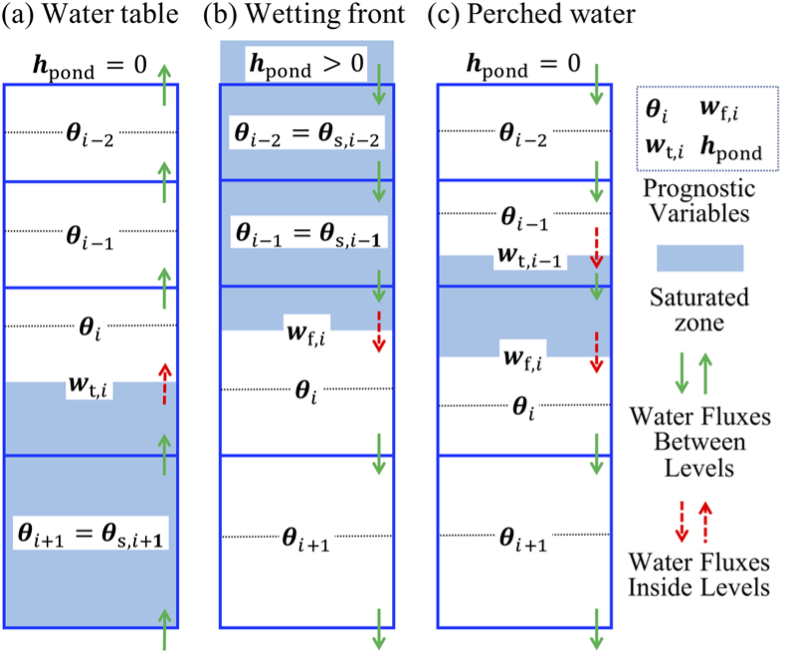
\includegraphics{Figures/陆地表面的水分循环/可变饱和流数值算法预报区域空间结构示意图.png}
\caption{可变饱和流数值算法预报区域空间结构示意图。}
\label{fig:可变饱和流数值算法预报区域空间结构示意图}
\end{figure}
}

\subsection{土壤水预报方程}
在每个土壤层内,有三个预报变量来描述土壤中液态水的分布情况。
土壤体积含水量为固定的预报变量($\theta_i$)。为了追踪土壤中饱和水层的变化(包括地下水、滞水层和入渗情况下由地表向下发展的饱和水层),
每层土壤中引入了另外两个潜在的预报变量($w_{f,i}$和$w_{t,i}$),
分别代表土壤层内上部饱和区域的厚度,和土壤层内下部饱和区域的厚度(图~\ref{fig:可变饱和流数值算法预报区域空间结构示意图}),
当某层土壤部分饱和时,这两个变量被激活。
{
\begin{figure}[]
\centering
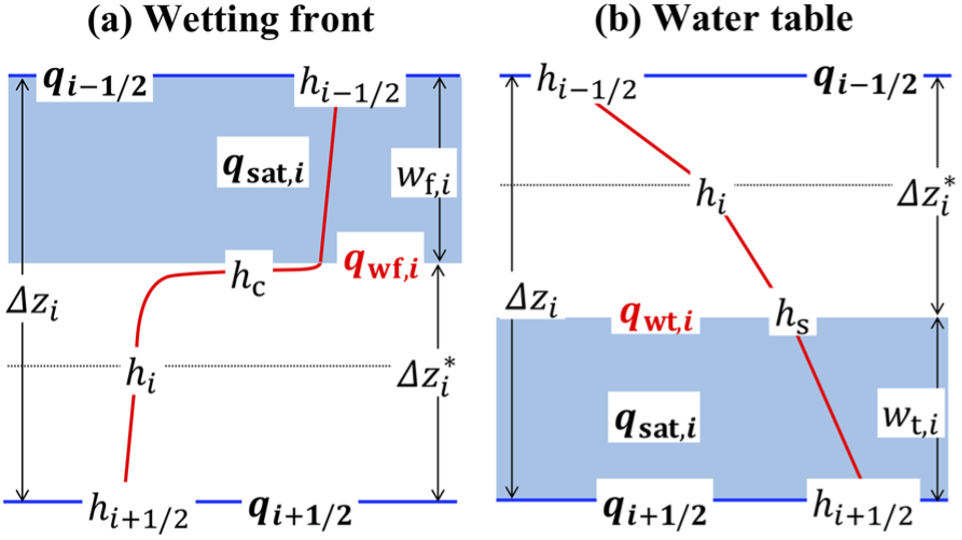
\includegraphics{Figures/陆地表面的水分循环/饱和-非饱和过渡状态的土壤层.png}
\caption{饱和-非饱和过渡状态的土壤层。如果土壤层内上部有饱和区(左图),
层内饱和区的厚度作为预报变量被激活;如果土壤层内下部有饱和区(右图),层内饱和区的厚度作为预报变量被激活。}
\label{fig:饱和-非饱和过渡状态的土壤层}
\end{figure}
}


预报变量($\theta_i$)的预报方程为
\begin{equation}\label{si_in1}
\left(\Delta z_{i}-w_{f, i}^{n+1}-w_{t, i}^{n+1}\right) \cdot\left(\theta_{i}^{n+1}-\theta_{i}^{n}\right)=\Delta t \cdot\left(q_{ {uin,i }}^{n+1}-q_{ {out }, i}^{n+1}\right)
\end{equation}
其中,$\Delta z_i$ 为第$ i $层土壤的厚度,$\Delta t$ 为时间步长,$q_{uin,i}^{n+1}$为非饱和区域上边界处的水流通量,$q_{out,i}^{n+1}$为非饱和区域下边界处的水流通量。


预报变量($w_{f,i}$)表示土壤层上部饱和区域的厚度,其预报方程为
\begin{equation}\label{si_in2}
\left(\theta_{s, i}-\theta_{i}^{n}\right) \cdot\left(w_{f, i}^{n+1}-w_{f, i}^{n}\right)=\Delta t \cdot\left(q_{i-1/2}^{n+1}-q_{w f, i}^{n+1}\right)
\end{equation}
其中,$\theta_{s,i}$ 为第$ i$ 层土壤的饱和体积含水量,$ q_{{i-1/2}}^{n+1}$为第$i$层土壤上边界处的水流通量,$q_{wf,i}^{n+1}$为饱和区域下边界处的水流通量。


预报变量($w_{t,i}$)表示土壤层下部饱和区域的厚度,其预报方程为
\begin{equation}\label{si_in3}
\left(\theta_{s, i}-\theta_{i}^{n}\right) \cdot\left(w_{t, i}^{n+1}-w_{t, i}^{n}\right)=\Delta t \cdot\left(q_{w t, i}^{n+1}-q_{i+1 / 2}^{n+1}\right)
\end{equation}
其中,$q_{wt,i}^{n+1}$  为饱和区域上边界处的水流通量,$q_{i+1/2}^{n+1}$为第$i$层土壤下边界处的水流通量。


在未饱和的土壤层,模式使用预报方程(\ref{si_in1})预报体积含水量的变化;
若未饱和的土壤层内上部有饱和区域,模式联合预报方程(\ref{si_in1})和(\ref{si_in2})来同时预报饱和区域的边界变化和非饱和区域内土壤积水含水量的变化;
若未饱和的土壤层内下部有饱和区域,模式联合预报方程(\ref{si_in1})和(\ref{si_in3})来同时预报饱和区域的边界变化和非饱和区域内土壤积水含水量的变化;
若未饱和的土壤层内上下部分均有饱和区域,模式联合预报方程(\ref{si_in1})--(\ref{si_in3})来同时预报饱和区域的边界变化和非饱和区域内土壤积水含水量的变化。


在地下部分,所有未饱和土壤层内的上述预报方程联合在一起组成一个方程组,来进行统一求解。

\subsection{地表积水的变化}
为了预报由入渗所产生的地表水深的变化,地表积水深度($h_{pond}$)也是算法中的预报变量,其预报方程为
\begin{equation}\label{hpond}
h_{ {pond }}^{n+1}-h_{ {pond }}^{n}=\Delta t \cdot\left(q_{ {surf }}^{n+1}-q_{ {infl }}^{n+1}\right)
\end{equation}
其中,$q_{surf}^{n+1} $ 为从地表水上部进入的水流通量,
其可以是降水、蒸发、或者地表水与积雪的液态水交换,$q_{infl}^{n+1}$为从地表进入土壤的水流通量。


当地表有积水,或者由于进入地表的水流通量大于入渗到土壤中的通量而形成积水时,积水深度的预报方程(\ref{hpond})也加入到土壤水的方程组中,进行统一求解。


\subsection{地下水的变化}
当地下水位在土壤水计算区域内部时,其位置由$w_{(t,i)}$进行预报。


当地下水位处于土壤水计算区域之下时,使用预报变量$W_a$来表示计算区域之下蓄水层的蓄水状态。$W_a$定义为
\begin{equation}
W_{a}=-\int_{z_{b t m}}^{Z_{w t}}\left(\theta_{s}-\theta\right) d z
\end{equation}
$W_a$的绝对值为土壤水计算区域之下单位面积上未填充液态水的孔隙的体积,
负号代表计算区域之下液态水是亏缺的。$W_a$的最大值为0,表示地下水位位于计算区域的下边界之上。


$W_a$的预报方程为
\begin{equation}\label{wa_n1_n}
W_{a}^{n+1}-W_{a}^{n}=\Delta t \cdot q_{b t m}^{n+1}
\end{equation}
当地下水位处于土壤水计算区域之下时,$W_a$的预报方程(\ref{wa_n1_n})也加入到土壤水的方程组中,进行统一求解。

\subsection{水流通量的计算}
预报方程(\ref{si_in1})(\ref{si_in2})(\ref{si_in3})(\ref{hpond})(\ref{wa_n1_n})中,右端项中均包含了水流通量的计算,其计算分为以下几种情形,
\begin{enumerate}
    \item 饱和区域内部的水流通量,使用公式
    \begin{equation}\label{q_sat1}
        q_{sat}=-\frac{\sum_{i=i_{1}}^{i_{2}} \Delta z_{i}}{\sum_{i=i_{1}}^{i_{2}} \frac{\Delta z_{i}}{K_{s, i}}}
         \cdot \frac{h_{l}-h_{u}-\sum_{i=i_{1}}^{i_{2}} \Delta z_{i}}{\sum_{i=i_{1}}^{i_{2}} \Delta z_{i}}
        \end{equation}
        其中,$i_1,i_1+1,…,i_2$为从上至下连续的饱和土壤层的层号,$\Delta z_i$为第i层的厚度,
        $K_(s,i)$为第$i$层的饱和土壤导水率,$h_l$为饱和区域下边界处的土壤水势。
        当饱和区域上边界为地表时,$h_u$取为地表积水深度$h_{pond}$;
        当饱和区域上边界在土壤内部时,$h_u$为饱和区域上边界处的土壤水势。
        (\ref{q_sat1})右端第一个分式计算了饱和区域的等效导水率,第二个分式计算了总水势的差商。

    \item 两个异质不饱和土壤层之间的水流通量,使用公式
    \begin{equation}\label{qht1}
        q_{h t}=q_{h m}\left(z_{i}-z_{u}, h_{u}, h_{i}\right)=q_{h m}\left(z_{l}-z_{i}, h_{i}, h_{l}\right)
        \end{equation}
        其中,$q_ht$为两层土壤间的水流通量,$z_u$为上层土壤的中心点的位置,$z_l$为下层土壤的中心点的位置,
        $z_i$为异质土壤的交界面的位置,$h_u$为$z_u$处的土壤水势,$h_l$为$z_l$处的土壤水势,$h_i$为$z_i$处的土壤水势。
        $q_{hm}$为计算均质土壤内水流通量的函数,它依赖于土壤层的厚度和上下边界处的土壤水势,
        (\ref{qht1})的含义为土壤层界面处的水流通量等于界面上方均质土壤内的水流通量,也等于界面下方均质土壤内的水流通量。
        土壤交界面处的土壤水势$h_i$为未知量,通过(\ref{qht1})的隐式方程进行求解后,再代入到(\ref{qht1})中计算$q_{ht}$. 函数$q_{hm}$为
        \begin{equation}
        q_{h m}\left(\Delta z, h_{u}, h_{l}\right)=-k_{h m} \cdot\left(\frac{h_{l}-h_{u}}{\Delta z}-1\right)
        \end{equation}
        其中,$\Delta z$为土壤层的厚度,$h_u$,$h_l$分别为土壤层上下两个边界处的土壤水势;
        $k_{hm}$为等效水力导度,其计算公式分为三种情况,对入渗情形($h_u>h_l$),
        \begin{equation}
        k_{h m}=\frac{1}{1-\frac{h_{l}-h_{u}}{\Delta z}} \cdot\left[k_{u}+\frac{h_{u}-h_{l}}{\Delta z}\left(k_{u}\right)^{1-r_{0}} \cdot\left(k_{l}\right)^{r_{0}}\right]
        \end{equation}
        对排水情形($h_l-\Delta z<h_u<h_l$),
        \begin{equation}
        k_{h m}=\left(k_{u}\right)^{r} \cdot\left(k_{l}\right)^{1-r}, r=\max \left(1+r_{0} \cdot \frac{h_{l}}{\Delta z}, 1-r_{0}\right)
        \end{equation}
        对毛细上升情形($h_u<h_l-\Delta z$),
        \begin{equation}
        k_{h m}=\left(k_{u}\right)^{r_{0}} \cdot\left(k\left(h_{l}-\Delta z\right)\right)^{1-r_{0}}
        \end{equation}
        其中,土壤水力导度$k$为土壤水势$h$的函数,上述三个公式中,$k_u=k(h_u )$,$k_l=k(h_l )$;
        $r_0$是依赖于土壤水力模型和土壤水力参数的参数,对Campbell模型,
        \begin{equation}
        r_{0}=\frac{1}{3 \lambda+2}
        \end{equation}
        对van Genuchten--Mualem模型,
        \begin{equation}
        r_{0}=\frac{1}{L(n-1)+2 n}
        \end{equation}
        预报方程(\ref{si_in1})(\ref{si_in2})(\ref{si_in3})为隐式时间积分格式,上述水流通量的计算公式可在理论上保证在均质土壤中,
        预报方程(\ref{si_in1})(\ref{si_in2})(\ref{si_in3})的解为本质无振荡的,也可在土壤具有分层异质性时,提高计算的稳定性和精度。

    \item 饱和区位于非饱和区上方时两者之间的水流通量,公式为
    \begin{equation}
    q_{w f}=q_{h m}\left(z_{l}-z_{i}, h_{s}, h_{l}\right)
    \end{equation}
    其中,$z_u$为上方非饱和土壤层中心点的位置,$z_i$为饱和区和非饱和区之间界面的位置,
    $h_s$为饱和土壤水势,$h_u$为非饱和土壤层中心点处的土壤水势。
\end{enumerate}


\subsection{预报方程的求解}
预报方程(\ref{si_in1})--(\ref{hpond})和(\ref{wa_n1_n})的左边均代表水量的变化,右边均代表土壤层边界上的水流通量,若在某时刻,
活动预报变量的个数为$A$,则可将第$\alpha$个变量对应的方程表达为
\begin{equation}\label{m_alpha_x}
\delta m_{\alpha}(\vec{x})=\Delta t \cdot \delta q_{\alpha}(\vec{x})
\end{equation}
其中$\vec{x}$⃗代表活动预报变量组成的向量,由(\ref{m_alpha_x})可得带约束的非线性最小二乘问题
\begin{equation}
\begin{aligned}
\min _{\vec{x}} f_{2}(\vec{x})=& \min _{\vec{x}} \sum_{\alpha=1}^{A}\left(\delta m_{\alpha}(\vec{x})-\Delta t \cdot \delta q_{\alpha}(\vec{x})\right)^{2} \\ 
& \theta_{r, i}<\theta_{i} \leq \theta_{s, i}, & \forall \theta_{i} \in \vec{x} \\ 
& 0 \leq w_{f, i} \leq \Delta z_{i},               & \forall w_{f, i} \in \vec{x} \\ 
& 0 \leq w_{t, i} \leq \Delta z_{i},               & \forall w_{t, i} \in \vec{x} \\ 
& h_{ {pond }} \geq 0,                               & \text{ if } h_{ {pond }} \in \vec{x} 
\end{aligned}
\end{equation}
此问题采用Gauss--Newton迭代算法进行求解。

\section{基于河道径流模式CaMa-Flood的汇流模拟}
汇流计算是通过耦合 Dai Yamazaki 等人于2011年提出的大尺度分布式汇流模型 CaMa-Flood (Catchment-based Macro-scale Floodplain) 实现的\citep{yamazaki2011physically}。
CaMa-Flood将全球河流网络分割为称为流域单元 (unit catchment) 的水文单元,在各单元集水区内利用河道 (river channel) 和漫滩 (floodplain) 的次网格 (subgrid) 
地形参数以及陆面模式生成的产流量 (total runoff),对总蓄水量 (total storage) 以及总流量 (total discharge) 进行预测,
并进一步实现对河道及漫滩流量 (river discharge and flood discharge),漫滩面积 (flood area) 以及平均漫滩水深 (flood depth) 
等日常所需的诊断量的高速计算。总蓄水量和总流量的时间演变通过求解局部惯性方程 \citep{bates2010} 得出。
CaMa-Flood同时考虑了上游单元的入流、下游单元的流出和每个流域单元的径流强迫输入,是目前高速求解河道水动力方程-圣维南方程最为高速有效的方法之一。
关于CaMa-Flood模型的详细描述可以从相关文献获取\citep{yamazaki2011physically,yamazaki2013improving,yamazaki2014regional,yamazaki2014development}。


CaMa-Flood 模型的主要优势之一在于除了能够精确描述河道径流以外,还能够模拟包括漫滩水位和漫滩面积变化等洪泛过程。
因此,对模拟结果的验证不仅仅局限于传统测量河流流量,还可以直接将模拟结果与卫星高度计对水面高程的观测以及微波成像仪对洪泛面积的估算进行比较;
能够有效加强全球河流模型各个输出的校准/验证\citep{yamazaki2012adjustment,yamazaki2012analysis}。
CaMa-Flood 模型的另一个优势在于它具有极高的模拟计算效率。通过引入次网格地形参数,复杂的漫滩淹没物理过程被合理地简化。
与此同时,通过实现局部惯性方程和自适应时间步长等物理方案\citep{bates2010},
河流流量和蓄水量的预测计算成本得到压缩,有利于进行集成/长期实验等计算要求高的实验或者与陆面模式之间的动态耦合。
以下对 CaMa-Flood 内部各个模块进行详细的介绍。目前耦合版本陆面过程模式分系统已经包含 CaMa-Flood v4.07版本。


\subsection{自适应时间步长的估算}
为避免固定时间步长计算所产生的数值振荡,提高数值方案稳定性,
CaMa-Flood 采用了\citet{bates2010}提出的基于局部惯性方程并满足 Courant-Friedrichs-Lewy (CFL) 
条件的自适应时间步长 ($DT_{adp}$) 的估算方法:
\begin{equation}
{DT}_{\max }=\boldsymbol{\alpha} \frac{\Delta x}{\sqrt{g h_{t}}}
\end{equation}
上式中$DT_{max}$是最大可接受的时间步长,$∆x$是该流域单元连接下游流域单元的河道长度 (river length) (m),
$\alpha$是稳定性系数设为0.9,$h_t$是该流域单元在时刻$t$的水流深度 (water depth) (m),$g$是重力加速度设为9.81 ($\rm m\,s^{-2}$)。
图~\ref{fig:自适应时间步长的估算} 展示了基于上述公式计算的某一时刻的$DT_{max}$ (minute)。
在计算过程中,如果用户指定的默认时间步长$DT$大于$DT_{max}$,则$DT$将被划分为满足$CFL$条件的更小的时间等分的时间步长$DT_{adp}$;
如果用户指定的默认时间步长$DT$小于$DT_{max}$,则实际计算步长按照用户指定的默认时间步长。
{
\begin{figure}[]
\centering
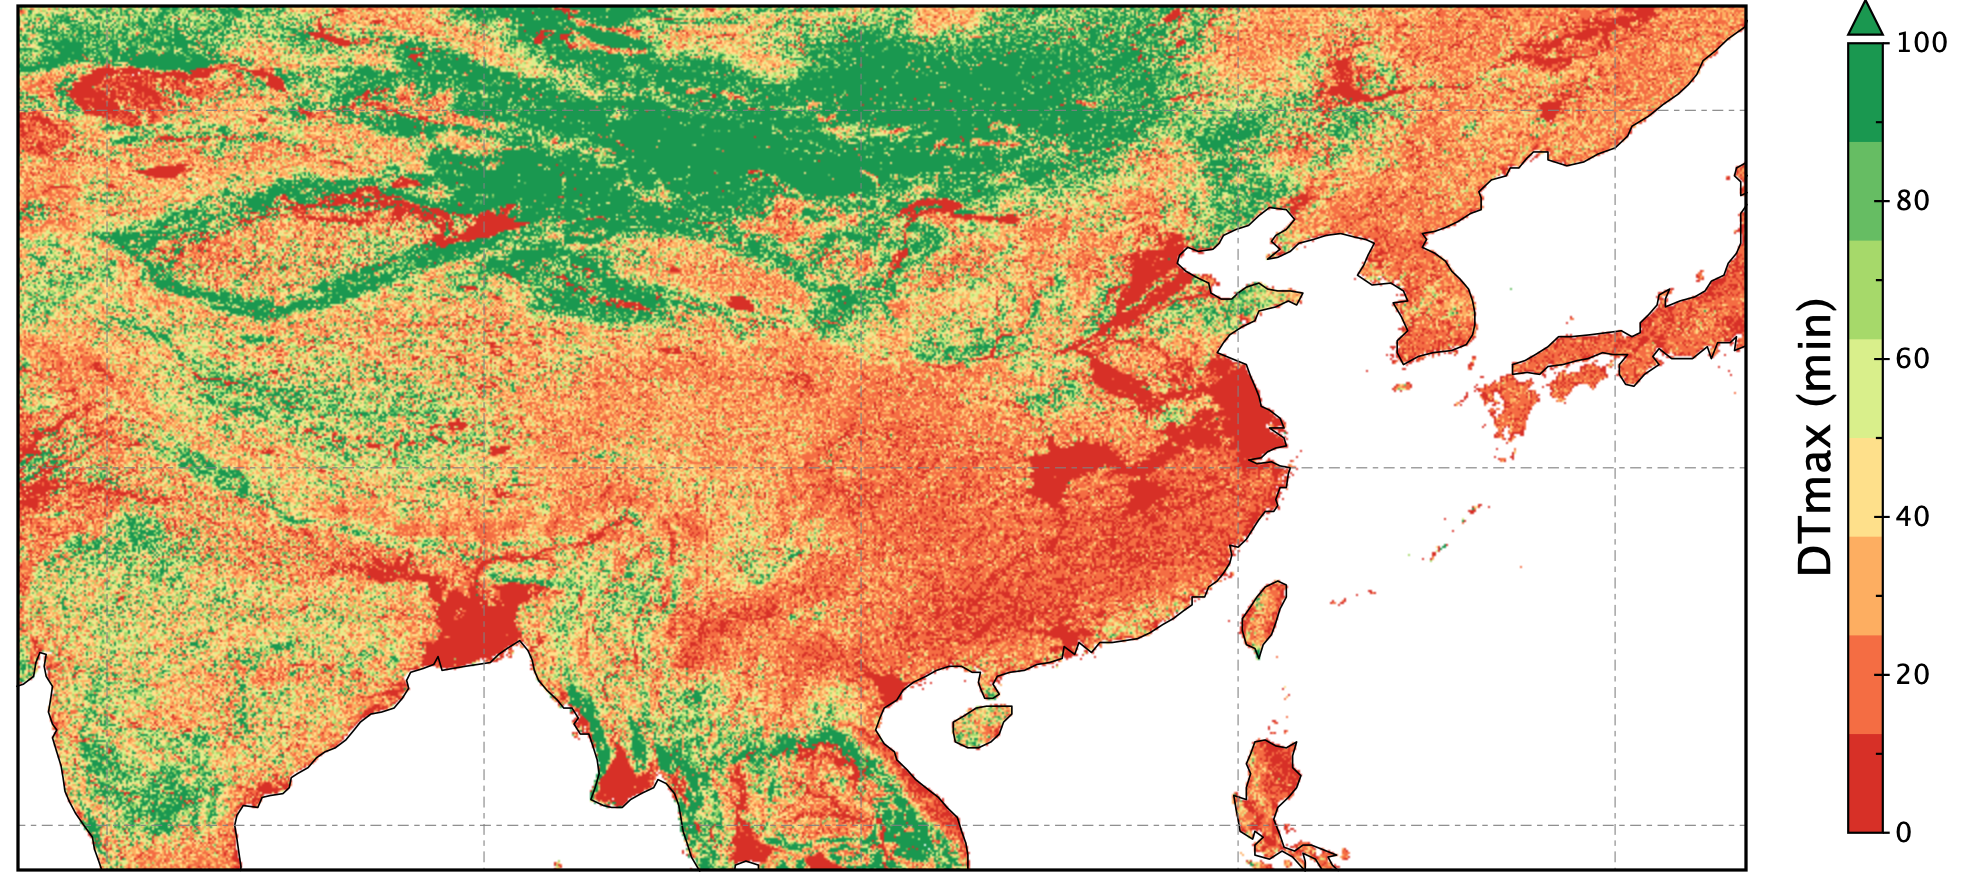
\includegraphics{Figures/陆地表面的水分循环/自适应时间步长的估算.png}
\caption{自适应时间步长的估算,摘自\citet{yamazaki2013improving}。}
\label{fig:自适应时间步长的估算}
\end{figure}
}


\subsection{诊断洪泛状态}\label{诊断洪泛状态}
在 CaMa-Flood 中指定网格的漫滩 (洪泛) 状态是通过计算该网格的蓄水总量得出的。如图~\ref{fig:CaMa-Flood流域单位示意图}
所示,河流河道蓄水量$S_r$,漫滩蓄水量$S_f$,河道水深度$D_r$, 漫滩淹没深度$D_f$,漫滩面积$A_f$等均通过求解基于总蓄水量的水量方程得出。
首先,模式中引发当前流域单元洪水蓄水量$S_{ini}$由如下公式进行确定:
\begin{equation}
S_{ ini }=B WL
\end{equation}
其中$B$是河道深度,$W$是河道宽度,及$L$是河道长度。如果总蓄水量$S$小于等于引发洪水蓄水量$S_{ini}$,
CaMa-Flood 假设不存在漫滩 (洪泛) 事件,上述参数则通过如下方程计算得出:
\begin{equation}
    \begin{array}{l}S_r=S \\ D_r=\frac{S_r}{WL} \\ S_f=0 \\ D_f=0 \\ A_f=0 \\ S_f=0\end{array}
\end{equation}
当总蓄水量$S$大于引发洪水蓄水量$S_{ini}$时,触发漫滩 (洪泛) 事件,则上述参数通过联立如下方程计算得出:
\begin{equation}
\begin{array}{l}S_r=S-S_f \\ D_r=\frac{S_r}{W L} \\ S_f=\int_{0}^{A_f}(D_f-D(A)) d_A \\ D_f=D_r-B \\ A_f=D^{-1}(D_f)\end{array}
\end{equation}
上式中的$D_f = D_r - B$表示河道与漫滩的水面高度相同。该方程是基于河道与漫滩之间的水量瞬间完成交换的假设。
函数$D^{-1}(D_f)$是漫滩高程剖面$D(A_f)$的反函数,它将泛滥地区$A_f$描述为漫滩水深$D_f$的函数 (见图~\ref{fig:CaMa-Flood流域单位示意图})。


{
\begin{figure}[]
\centering
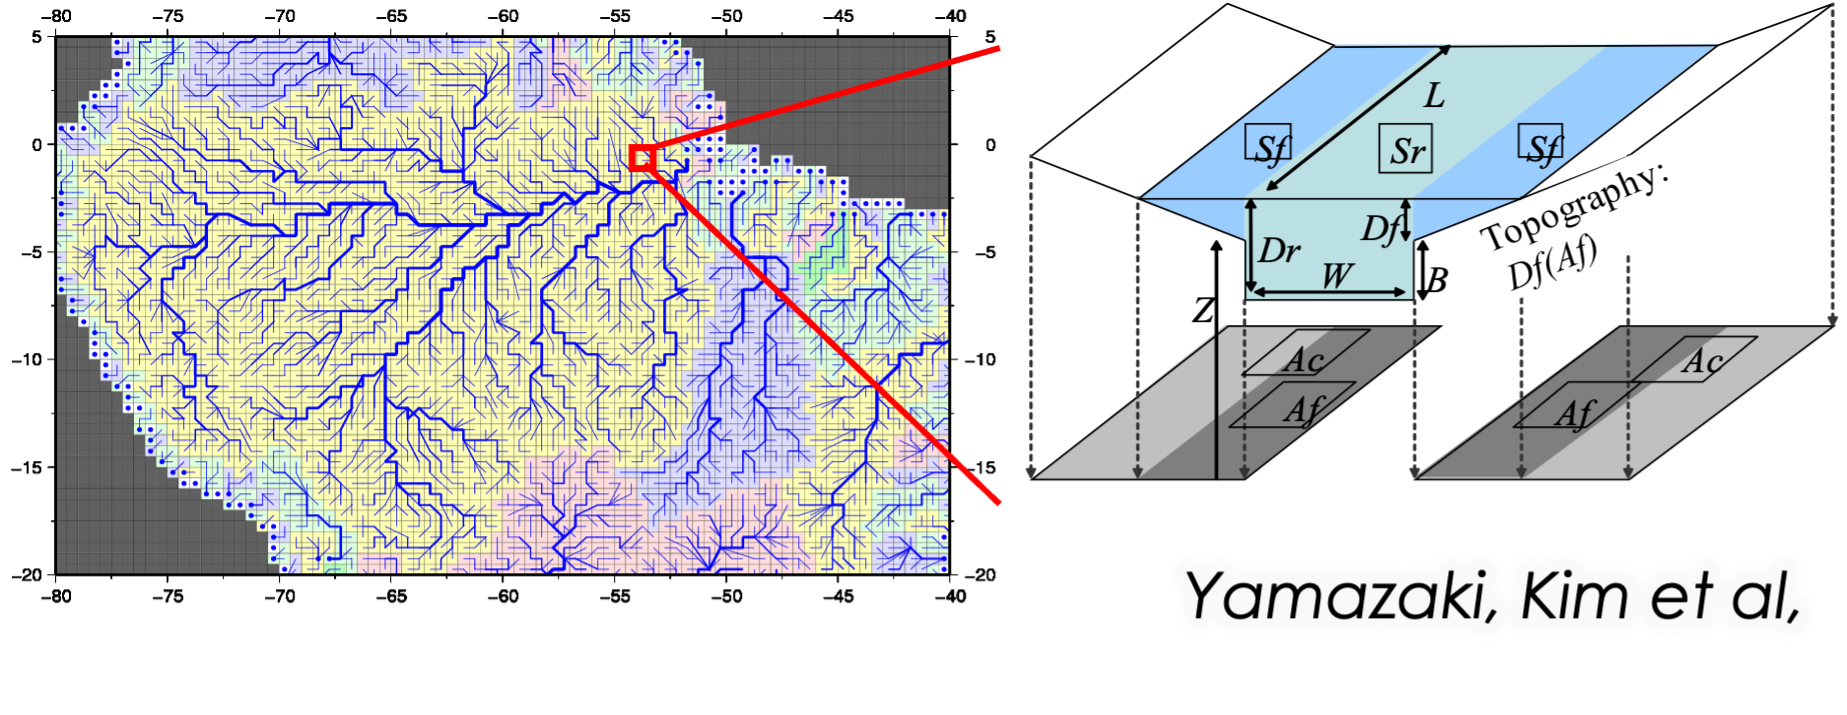
\includegraphics{Figures/陆地表面的水分循环/CaMa-Flood流域单位示意图.png}
\caption{CaMa-Flood流域单位示意图,摘自\citet{yamazaki2011physically}。 }
\label{fig:CaMa-Flood流域单位示意图}
\end{figure}
}

\subsection{河道径流流量计算}
CaMa-Flood 分别计算了各流域单元向其下游单元的河流径流量和漫滩流量。
二者的计算均通过忽略如下 St. Venant 动量方程式第二项,得到径流计算所使用的局部惯性方程 \cite{bates2010}:
\begin{equation}
\frac{\partial Q}{\partial t}+\frac{\partial}{\partial x}\left[\frac{Q^{2}}{A}\right]+\frac{g A \partial(h+z)}{\partial x}+\frac{g n^{2} Q^{2}}{R^{4 / 3} A}=0
\end{equation}
式中$Q$为河流流量 ($\rm m^3s^{-1}$),$A$为水流横截面面积 ($\rm m^2$),$h$为水流深度 (m),$z$为河床高程 (m),
$R$为水力半径 (m),$g$为重力加速度 ($\rm m s^{-2}$),$n$为曼宁摩擦系数($\rm m^{-1/3} s^{-1}$)。
$x$和$t$分别为流动距离和时间。第一项、第二项、第三项和第四项分别表示局部加速度、平流、水面坡度和摩擦坡度。CaMa-Flood模型采用局部惯性方程的显式形式: 

\begin{equation}
Q^{t+\Delta t}=\frac{Q^{t}+\Delta t g A i S}{1+\frac{\Delta t g n^{2}\left|Q^{t \mid}\right|}{R^{4 / 3} A}}
\end{equation}
其中$S$是水面坡度,$Q^t$为当前时刻的流量, $Q^{t+\Delta t}$是单位时间间隔 $\Delta t$ 之后的流量。水力半径 $R$ 近似为水流深度。曼宁系数默认设置为$n=0.03$。
在局部惯性方程计算中可能出现的负向河流量,代表了下游流域单元向当前流域单元的反向水流(回水)。同时为防止当前网格的总的流出量超过蓄水量,
CaMa-Flood 引入限流器的概念:当总出水量大于网格的总库存量时,CaMa-Flood 使用修正系数对径流流量进行修正。


\subsection{河道径流流量计算}
漫滩流量计算与河道径流流量计算方法相同。
其区别在于漫滩流量包括所使用的水流面积$A$的计算方法是漫滩蓄水量除以河道长度;
水流深度$h$为漫滩深度;漫滩流量的曼宁系数被设置为$n=0.10$。

\subsection{蓄水量变化计算}
{
\begin{figure}[]
\centering
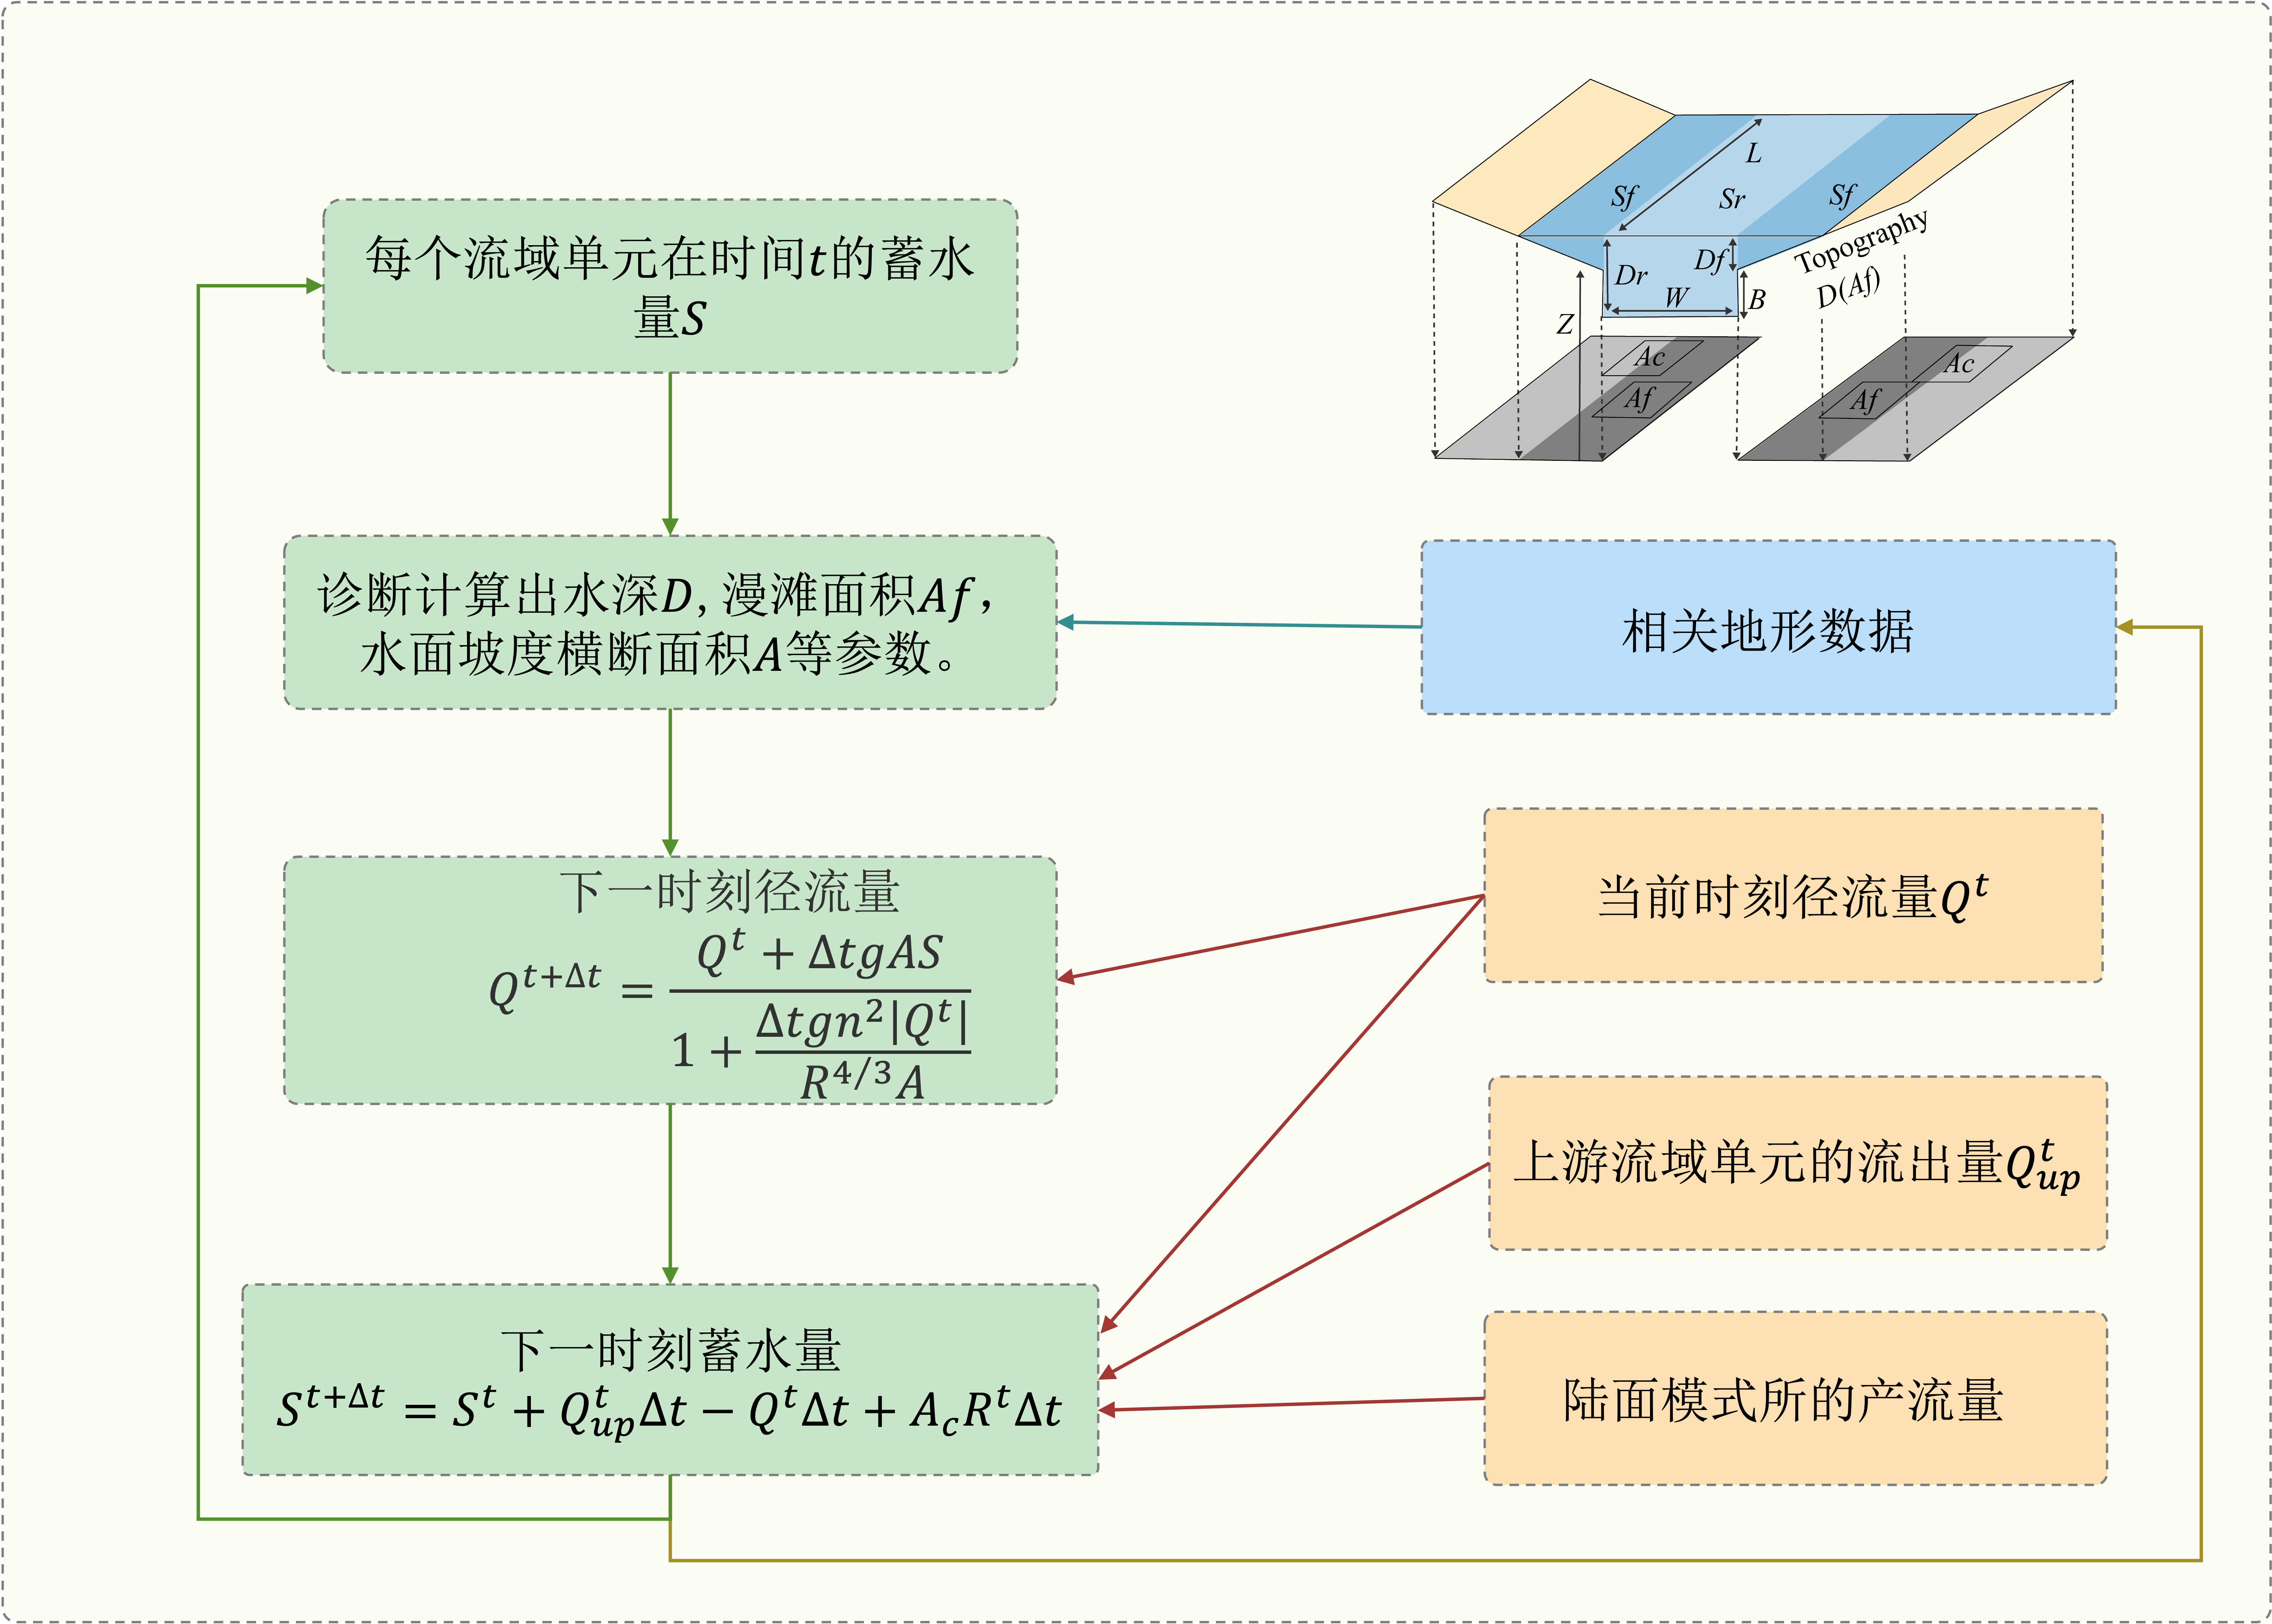
\includegraphics{Figures/陆地表面的水分循环/蓄水量变化计算流程图.png}
\caption{蓄水量变化计算流程图。 }
\label{fig:蓄水量变化计算流程图}
\end{figure}
}
蓄水量随时间的变化的计算流程如图~\ref{fig:蓄水量变化计算流程图}所示,指定流域单元的蓄水量变化的计算基于质量平衡方程:
\begin{equation}
S_{i}^{t+\Delta t}=S_{i}^{t}+\sum_{k}^{Upstream} Q_{k}^{t} \Delta t-Q_{i}^{t} \Delta t+A c_{i} R_{i}^{t} \Delta t
\end{equation}
式中$S_{i}^{t}$和$S_{i}^{t+\Delta t}$分别代表单元$i$在时间$t$到时间$t+\Delta t$蓄水量的变化,$Q_i^t$代表在时间$t$该单元河流径流出流量 (河道内+漫滩),
$Q_k^t$代表在时间 $t$ 该单元从上游网格接收的河流径流流入流量 (河道内+漫滩),$Ac_i$ 是单元$i$的面积,$R_i^t$ 代表流域单元 $i$ 的产流量。

\subsection{河网地图}
CaMa-Flood 模拟所需的相关次网格地形参数是由 90m 超高精细分辨率的全球流动方向地图 (MERIT-Hydro)\citep{yamazaki2019merit},
水文调整高程 DEM \citep{yamazaki2017high,yamazaki2012analysis},以及河宽数据\citep{yamazaki2014development}; 
使用 \citet{yamazaki2009deriving} 开发的升尺度模式 Flexible Location of Waterways (FLOW) 计算得出。
相关数据以纯``二进制''格式 ($nx*ny$)存储于 \texttt{map/} 目录下。默认的数据存储顺序是从180 \textdegree W到180 \textdegree E,
从 90 \textdegree N 到 90 \textdegree S;数据的字节顺序是 ``little endian''。
具体而言,除了需要陆面模式计算得出的产流量 (runoff) 之外,CaMa-Flood还需要包括流域面积 ($A_s$),河道长度 ($L$),河道宽度 ($W$) 及深度 ($B$),
漫滩 (洪水淹没) 面积,以及用于计算平均漫滩水深的漫滩高程剖面等相关的次网格地形数据。除了河流的宽度和深度以外,
所有的地形相关参数均可由 MERIT-hydro 水文地形数据中获取。以下以全球 0.25\textdegree 的河网为例进行详细介绍。

{
\begin{figure}[]
\centering
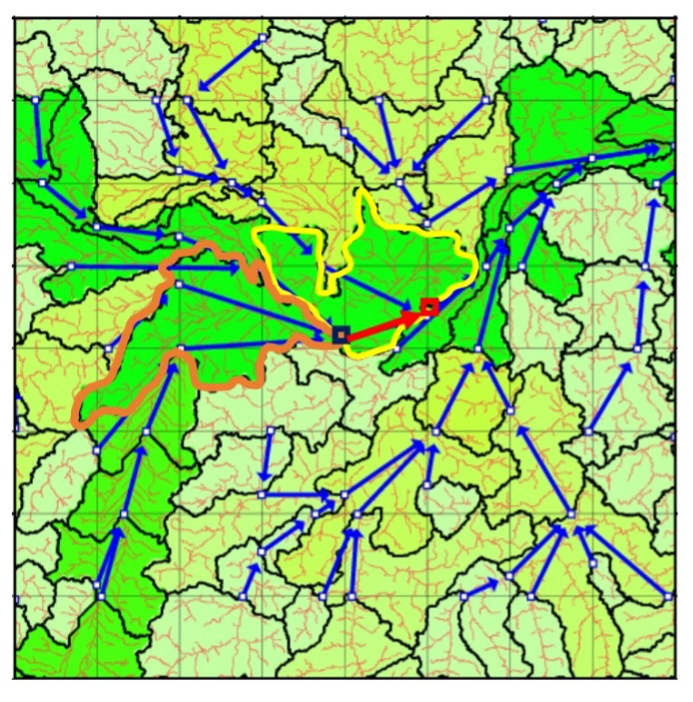
\includegraphics{Figures/陆地表面的水分循环/流域单元分布图.png}
\caption{流域单元分布图。每个流域单元的出口用白色四边形标记。蓝色线条连接不同流域单元,箭头指向下游流域单元。
橙色和黄色边界代表了不同的流域单元。图片摘自\citet{yamazaki2013improving}。 }
\label{fig:流域单元分布图}
\end{figure}
}


在目录\texttt{glb\_15min}下包含了全球 0.25\textdegree 分辨率的网格-矢量-混合 (grid-vector-hybrid) 河网图,
该河网地图是由 90m MERIT Hydro 数据使用 FLOW 模式升尺度而来 (图~\ref{fig:流域单元分布图});
具体文件内容如表~\ref{tab:河网图及地形参数文件列表}和表~\ref{tab:河网图及地形参数文件列表2} 所示。
河网地图的维度信息,包括东西方向网格数目$nx$,南北方向网格数目$ny$,泛滥平原层数 ($nfpl$),
网格大小 ($gsize$)和区域边界 (西、东、南、北),记录在 \texttt{params.txt} 之中。\texttt{nextxy.bin} 文件包含了2个参数 ($nextx$和$nexty$),
分别记录了每个网格的下游单元的相对位置,
其中与海洋接口的河口标记为 -9,内陆河流终点标记为 -10,海洋 (未定义) 标记为 -9999。

% Please add the following required packages to your document preamble:
% \usepackage{booktabs}
\begin{table}[]
\centering
\caption{河网图及地形参数文件列表}
\label{tab:河网图及地形参数文件列表}
    \begin{tabular}[h]{p{3.5cm}p{1.5cm}p{1.5cm}p{5cm}p{1cm}p{1cm}}  %{@{}cccccc@{}}
    \toprule
    File              & Variable & Symbol                        & Description                                  & Unit    & Format  \\ \midrule
    \texttt{params.txt}        & -        & -                             & Map parameters                     & -         & text    \\
    \texttt{nextxy.bin}        & \texttt{nextx}    & $jx$                         & Downstream X (rec=1)         & -         & integer \\
                                       & \texttt{nexty}    & $jy$                         & Downstream Y (rec=2)            & -        & integer \\
    \texttt{downxy.bin}      & \texttt{downx}   & $dx$                        & Relative DownstreamX (rec=1)   & -   & integer \\
                                       & \texttt{downy}   & $dy$                      & Relative Downstream Y (rec=2)   & -    & integer \\
    \texttt{ctmare.bin}       & \texttt{ctmare}   & $Ac$                     & Unit-catchment Area                     & $\rm m^2$   & real    \\
    \texttt{elevtn.bin}        & \texttt{elevtn}    & $Z$                        & Base Elevation                         & m       & real    \\
    \texttt{rivlen.bin}         & \texttt{rivlen}    & $L$                         & Channel Length                        & m       & real    \\
    \texttt{rivhgt.bin}         & \texttt{rivhgt}   & $B$                         & Channel Depth                          & m       & real    \\
    \texttt{rivwth.bin}        & \texttt{rivwth}   & $W$                        & Channel Width                           & m       & real    \\
    \texttt{rivwth\_gwdlr.bin} & \texttt{rivwth}   & $W$                    & Combined Width (recommended)    & m       & real    \\
    \texttt{nxtdst.bin}        & \texttt{nxtdst}   & $X$                             & Downstream Distance                          & m       & real    \\
    \texttt{fldhgt.bin}        & \texttt{fldhgt}   & $D_f$                            & Floodplain Elevation profile (rec=1$\sim$10) & m       & real    \\
    \texttt{rivman.bin}        & \texttt{rivman}   & -                             & Manning’s Roughness                          & -       & real    \\
    \texttt{bifori.txt}        & -        & -                             & Bifurcation Channel Original Data            & -       & text    \\
    \texttt{bifprm.txt}        & -        & -                             & Bifurcation channel parameters               & -       & text    \\ \bottomrule
    \end{tabular}
\end{table}


    % Please add the following required packages to your document preamble:
% \usepackage{booktabs}
\begin{table}[]
\centering
\caption{河网图及地形参数文件列表续}
\label{tab:河网图及地形参数文件列表2}
    \begin{tabular}[h]{p{3.5cm}p{1.5cm}p{1.5cm}p{5cm}p{1cm}p{1cm}} %{@{}cccccc@{}}
    \toprule
    File             & Variable & Symbol                             & Description                                          & Unit     & Format  \\ \midrule
    \texttt{grdare.bin}       & \texttt{grdare}   & -                                  & Rectangular grid area (optional)                     & $\rm m^2$       & real    \\
    \texttt{nxtdst\_grid.bin} &          &                                    &                                                      &          &         \\
    \texttt{rivlen\_grid.bin} & \texttt{nxtdst}   & $X$                                  & Downstream Distance (grid center)                    & m        & real    \\
                                        & \texttt{rivlen}    & $L$                            & Channel Length (grid center)       &    m                             & real        \\
    \texttt{inpmat.bin}       & \texttt{inpx}     & -                                  & Corresponding input grid X (rec=1) & -        & integer \\
                                       & \texttt{inpy}     & -                               & Corresponding input grid Y (rec=2)    & -        & integer  \\
    \texttt{ctmare.bin}       & \texttt{inpa}     & $A_{ij}$                            & Area of input grid XY (rec=3)              & $\rm m^2$     & real    \\
    \texttt{diminfo.txt}      & -        & -                                  & Dimension infomation                         & text     &         \\
    \texttt{lsmask.bin}       & -        & -                                  & Land ID of corresponding hi resolution area Basin ID & -        & integer \\
    \texttt{basin.bin}        & -        & -                                  & Basin ID                                             & -        & integer \\
    \texttt{bsncol.bin}       & -        & -                                  & Basin Color Pattern for Visualization                & -        & integer \\
    \texttt{lonlat.bin}       & \texttt{lon}      & -                                  & Longitude, catchment outlet (rec=1)     & \textdegree      & real    \\
                                     & \texttt{lat}       & -                                 & Latitude, catchment outlet (rec=2)        & \textdegree       & real    \\
    \texttt{uparea.bin}       & \texttt{uparea}   & -                           & Upstream Drainage Area                       & $\rm m^2$        & real    \\ \bottomrule
    \end{tabular}
\end{table}


假设任意网格的洪水事件是从高程低的区域到高程高的区域发生淹没,
任意流域单元(图~\ref{fig:基于流域单元的漫滩高程剖面函数}) 的漫滩面积可以由漫滩水深$D_f$ (m) 
以及累积分布函数 (CDF) 的经验函数生成 (图~\ref{tab:河网图及地形参数文件列表2})。
每个网格的CDF函数的第10百分位数的10个值 (图~\ref{tab:河网图及地形参数文件列表2},红色圆点)分别存储在 \texttt{fldhgt.bin} 的十个参数之中
 (见表~\ref{tab:河网图及地形参数文件列表}和表~\ref{tab:河网图及地形参数文件列表2}),文件格式与上述的 \texttt{nextxy.bin} 相同。
例如,\texttt{fldhgt.bin} 的第三个参数表示流域单元 30\% 的面积被淹没时的该流域单元的平均洪水深度 (m)。

{
\begin{figure}[]
\centering
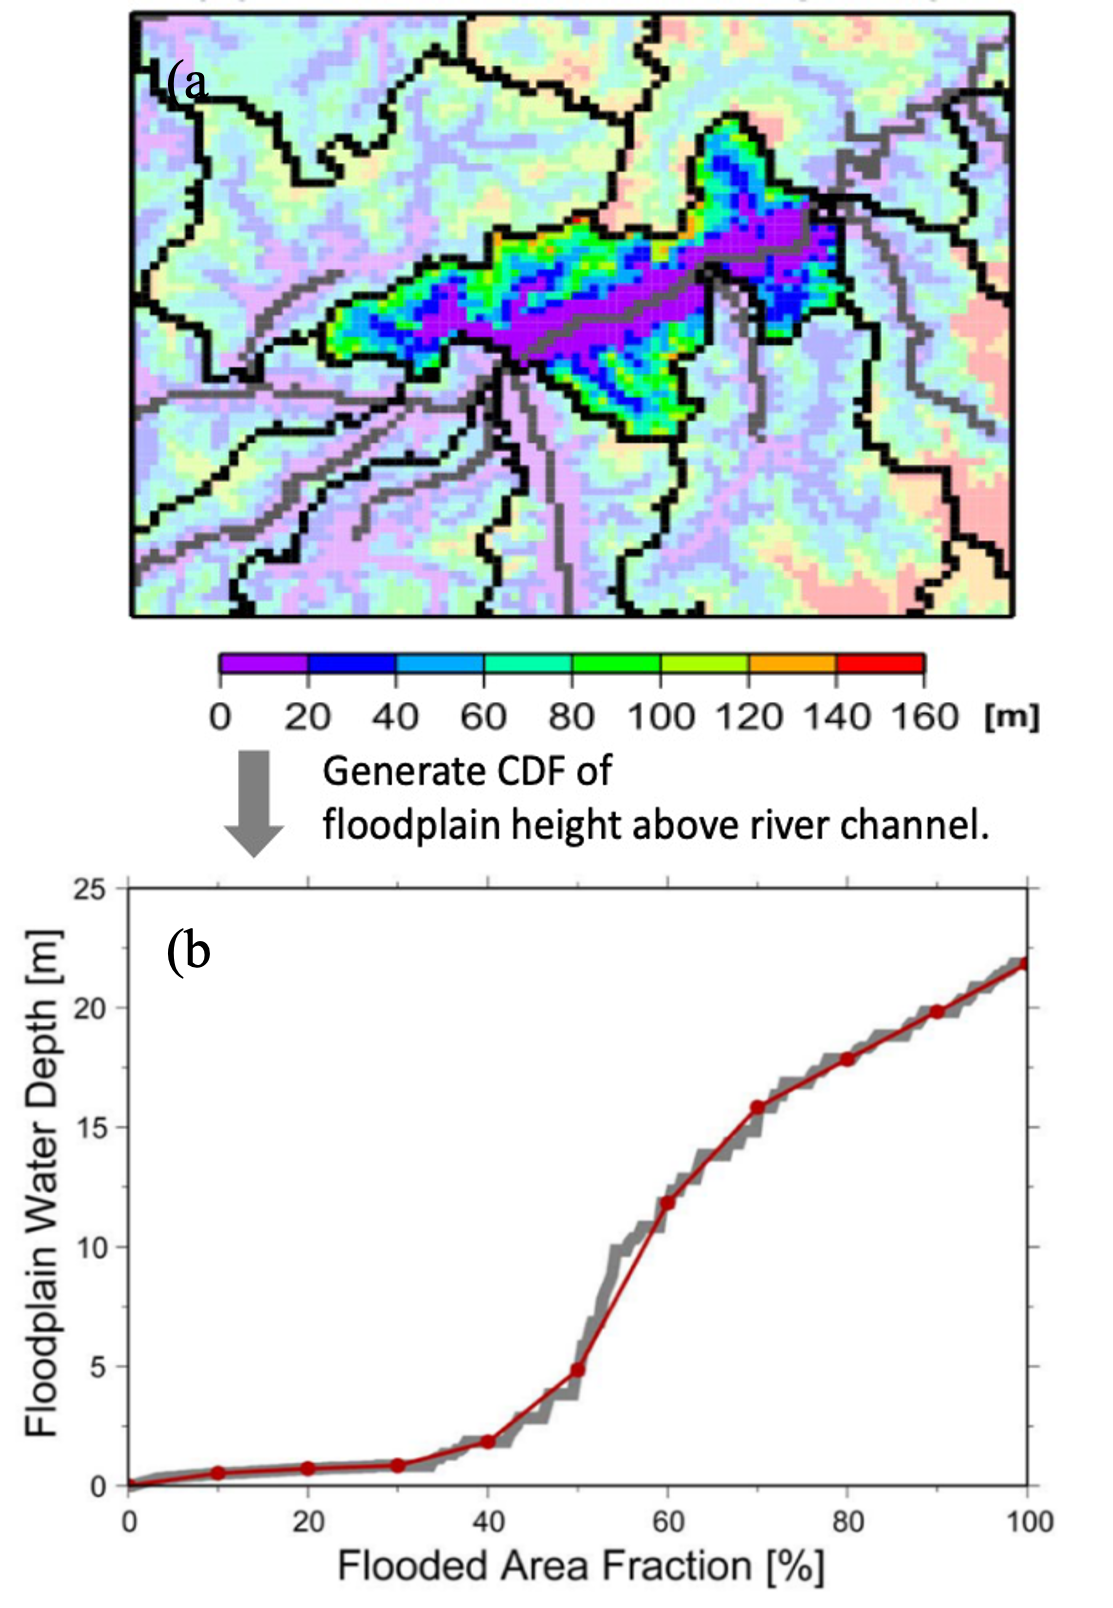
\includegraphics{Figures/陆地表面的水分循环/基于流域单元的漫滩高程剖面函数.png}
\caption{基于流域单元的漫滩高程剖面函数。图片摘自\citet{yamazaki2013improving}。  }
\label{fig:基于流域单元的漫滩高程剖面函数}
\end{figure}
}


河道断面参数(河道长度$W$ (m)和河道深度 $B$ (m))是水动力模拟的主要参数之一。在CaMa-Flood中的该参数是流域产流量的气候态的经验函数,由以下公式推导得出:
\begin{equation}
W=\max \left(W_{min}, c_{w} * Q_{ave}{}^{p_{w}}+W_{0}\right)
\end{equation}
\begin{equation}
B=\max \left(B_{min}, c_{H} * Q_{ave}{}^{p_{H}}+B_{0}\right)
\end{equation}
其中$Q_{ave}$是由陆面模式计算得出的产流量 (total runoff) ($\rm m^3\,s^{-1}$)。
河道宽度计算所使用的经验系数 $c_w$,$p_w$,$W_0$,$W_{min}$ 分别设置为 2.5,0.6,0.0 以及5.0;
河道深度计算所使用的经验系数 $c_H$,$p_H$,$B_0$ 和 $B_{min}$ 分别设置为 0.1,0.5,0.0 以及1.0。
值得注意的是这些经验系数存在着极大的不确定性,在使用之时需要对其进行对应的率定和调参。
除此之外,基于卫星观测的河道宽度数据 (\texttt{width.bin},如图~\ref{fig:基于卫星数据生成的河道宽度示意图}) 也可由MERIT-hydro水文地形数据中获取。
CaMa-Flood推荐使用通过 \texttt{set\_gwdlr.F90} 子程序生成组合宽度参数 (经验公式和卫星数据的组合) 数据。
相关地图的制备详见 \citet{yamazaki2014regional, yamazaki2014development}。
{
\begin{figure}[]
\centering
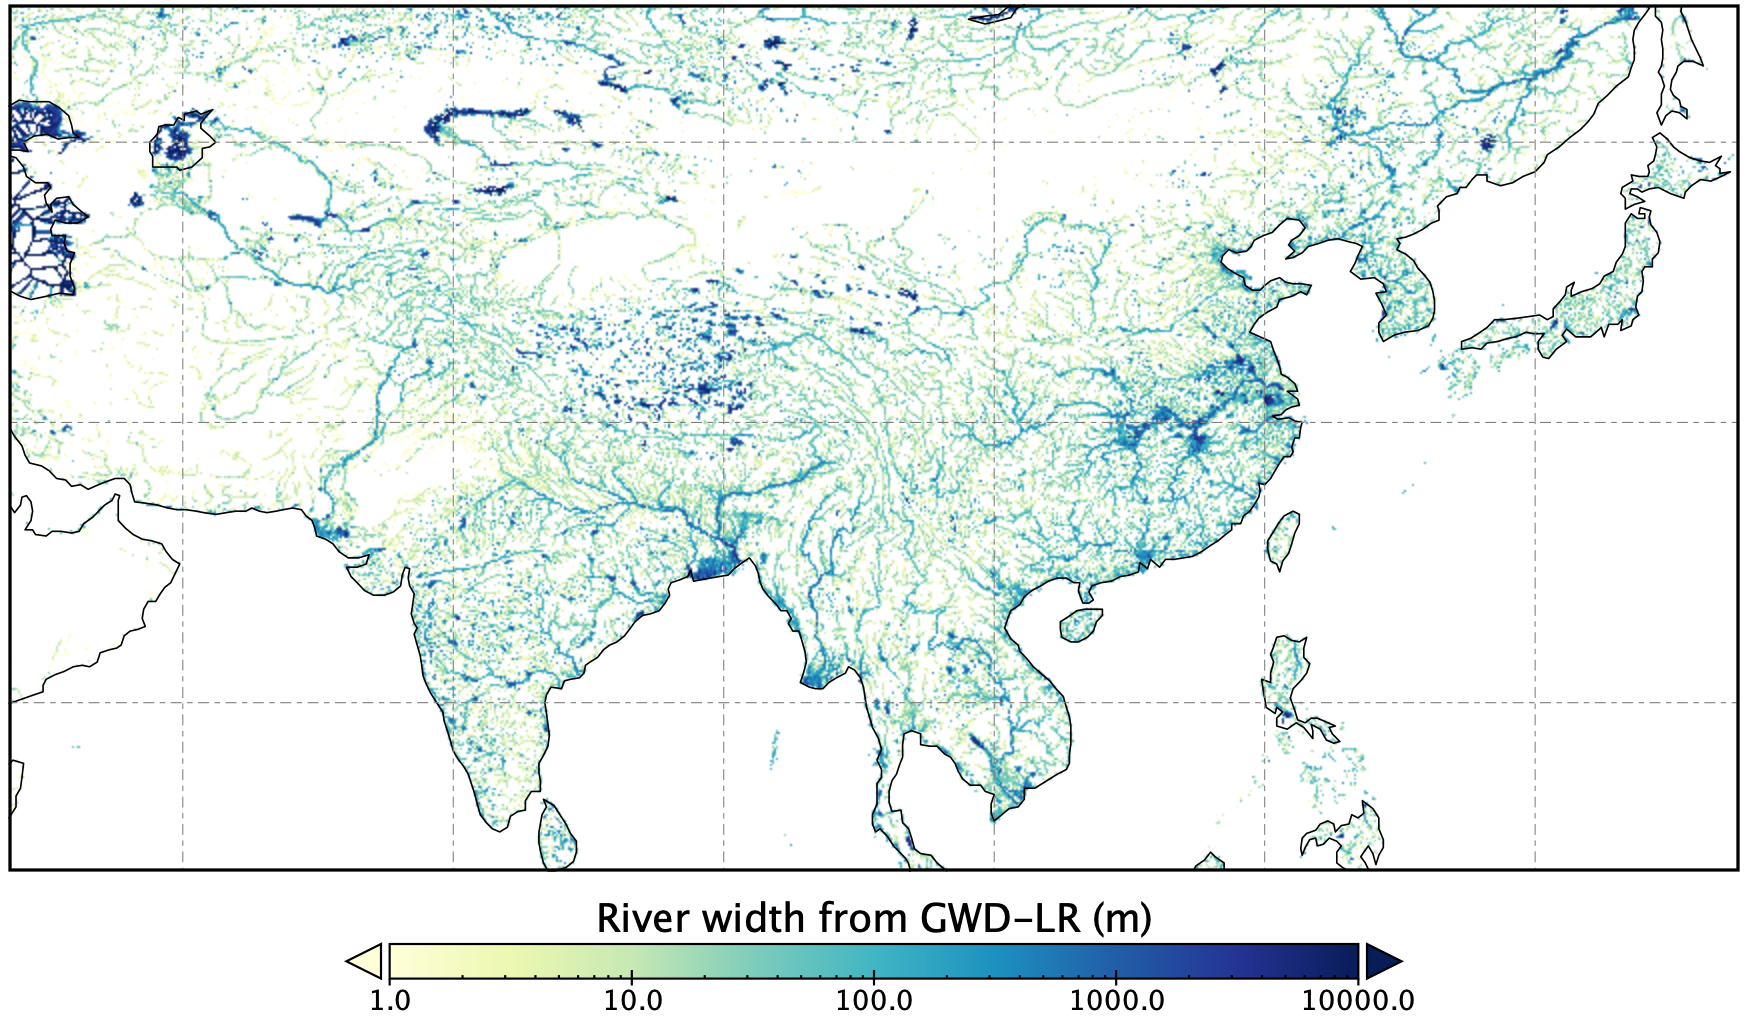
\includegraphics{Figures/陆地表面的水分循环/基于卫星数据生成的河道宽度示意图.png}
\caption{基于卫星数据生成的河道宽度示意图。图片摘自\citet{yamazaki2011physically}。}
\label{fig:基于卫星数据生成的河道宽度示意图}
\end{figure}
}

如图~\ref{fig:CaMa-Flood流域单位示意图} 所示,由于 CaMa-Flood 是基于流域单元进行计算的,而陆面模式是基于规则的经纬度网格,
流域单元在当前陆面模式分辨率 (经纬度网格) 投影下呈现不规则的形状。
因此在流域边缘有可能出现一个网格分属于不同流域,以及多个经纬度网格单元同属于一个流域单元的情况。
这就需要强制插值分割这些陆面模式经纬度网格生成的产流量到不同的流域。
指定流域单元$i$从陆面模式网格获得的水量由如下公式进行计算:
\begin{equation}
F_{i}=\sum_{N} A_{i, j} R_{j}
\end{equation}
其中$F_i$为进入流域单元$i$在单位时间 [$\rm m^3\,s^{-1}$]的输入水量,$A_{i, j}$ 是陆面模式的经纬度网格单元$j$在属于指定流域单元的面积大小,
 $N$是指属于指定流域单元陆面模式的经纬度网格的数量。该映射信息被存储在 \texttt{test\_***.bin} (\texttt{***} 是网格分辨率
 ,例如 \texttt{test\_1deg.bin})。同时,还需准备一个文本文件 (比如说 \texttt{diminfo\_test-1deg.txt}) 用来指定模拟的维度
  (比如说区域,分辨率,流域单元数量,输入经纬度网格数量,输入的映射文件名 \texttt{test\_***.bin})。

在 \texttt{map} 目录中,CaMa-Flood 还准备了一些用于生成映射矩阵和漫滩高程剖面曲线所需的高分辨率数据 (如 \texttt{3sec},\texttt{1min},\texttt{15min},
\texttt{3min} 等目录之下)。
高分辨率数据被划分为\texttt{\$(TILE).\$(VAR).bin},每个TILE的区域记录在 \texttt{location.txt} 文件之中;
具体提供的参数 \texttt{\$(VAR)} 如表~\ref{tab:河网图及地形参数文件列表2} 所示。其中 \texttt{\$(TILE).flwdir.bin} 和
\texttt{\$(TILE).downxy.bin} 分别以基于 D8 格式和 downstreamXY 格式描述了河流流向;\texttt{\$(TILE).catmzy.bin} 表示流域单元内的网格 (ix, iy) 
在高分辨率经纬度网格 (iXX, iYY)上的映射;\texttt{\$(TILE).catmzz.bin} 表示每个网格对应的漫滩层;\texttt{\$(TILE).flddif.bin} 表示每个网格堤坝平均高度 [m],
用于对粗分辨率的漫滩水深进行降尺度;\texttt{\$(TILE).visual.bin} 用于高分辨率流域边界可视化,其中数值上体现为海洋 = 0, 
陆地 (未调整) = 1, 陆地 (调整并在 CaMa 中使用) = 2, 通常网格 = 3,流域边界 = 5, 河道 = 10, 内陆流域出口 = 20, 与海洋连接的河口 = 25。
具体文件列表见表~\ref{tab:河网各数据文件}。

% Please add the following required packages to your document preamble:
% \usepackage{booktabs}
\begin{table}[]
    \centering
    \caption{河网各数据文件}
    \label{tab:河网各数据文件}
    \begin{tabular}[h]{p{4cm}p{1.5cm}p{1.5cm}p{4cm}p{1cm}p{2cm}} %{@{}cccccc@{}} %
    \toprule
    File                & Variable    & Symbol                        & Description                   & Unit      & Format \\ \midrule
    \texttt{location.txt}        & -        & -                             & Hi-res domain info            & -         & text   \\
    \texttt{\$(TILE).catmxy.bin} & \texttt{catmx}    & $iXX$         & catchment (iXX,jYY) rec=1     & - & int*2byte       \\
                                               & \texttt{catmy}    & $jYY$      & catchment (iXX,jYY) rec=2     & - & int*2byte      \\
    \texttt{\$(TILE).catmzz.bin} & \texttt{catmz}    & -                 & floodplain layer              & -  & int*1byte \\
    \texttt{\$(TILE).flwdir.bin} & \texttt{dir}      & -                        & flow direction (D8)         & -   & int*1byte  \\
    \texttt{\$(TILE).downxy.bin} & \texttt{downx}    & $dx$          & relative downstream x (rec=1) & - & int*2byte   \\
                                                & \texttt{downy}    & $dy$       & relative downstream y (rec=2) & - & int*2byte   \\
    \texttt{\$(TILE).elevtn.bin}    & -        & -                             & elevation                     & m                             & real    \\
    \texttt{\$(TILE).flddif.bin}      & -        & -                             & height above river channel    & m                             & real   \\
    \texttt{\$(TILE).rivwth.bin} & -        & -                                & river channel width           & m                             & real   \\
    \texttt{\$(TILE).grdare.bin} & -        & -                               & pixel area                    & $\rm m^2$                            & real   \\
    \texttt{\$(TILE).uparea.bin} & -       & -                               & upstream drainage area        & $\rm m^2$       & real   \\
    \texttt{\$(TILE).visual.bin}  & -        & -                               & Catchment visualization        & -                                                        & int*1byte       \\ \bottomrule
    \end{tabular}
\end{table}


\section{考虑水库影响的河道汇流}
    本模块在CaMa-Flood中实施水库运行方案,通过识别坝体所在的集水区单元,
    根据水库运行规则计算水库流出量,构建考虑大坝影响的河道汇流参数化方案,
    以刻画水库对陆面水文循环过程的影响。
    
\subsection{水库数据集和水库参数估计}\label{水库数据集和水库参数估计}
大坝水库的基本信息来自全球大坝水库数据集 GRanD \citep{lehner2011high},GRanD version 1.3 包含全球 7320 座大坝及其相关水库的数据。
本模块需使用数据库中的大坝名称、坝体坐标、总库容和流域面积等信息,然后在 CaMa-Flood 河网上定位水库,并估算水库特征参数。
水库的定位程序包括以下几个步骤:首先根据水库的地理参考坐标计算相应的网格坐标,然后使用河网数据对水库位置进行了校正,
具体来说,将初始水库网格的集水面积与实际值进行比较,如果相对误差大于 10\%,
则对网格的位置进行调整,在周围八个网格进行搜索将流域面积误差降至最低,以此类推直到误差小于10\%。
此外,如果多个水库位于河网中的单个网格中,则模型只选择总蓄水量最大的水库而删除其他水库。通过上述步骤,
在 0.25\textdegree 河网中共计识别到 2169 座水库,在 0.05\textdegree 河网中共计识别到 5715 座水库(图~\ref{fig:水库分布})。

{
\begin{figure}[]
\centering
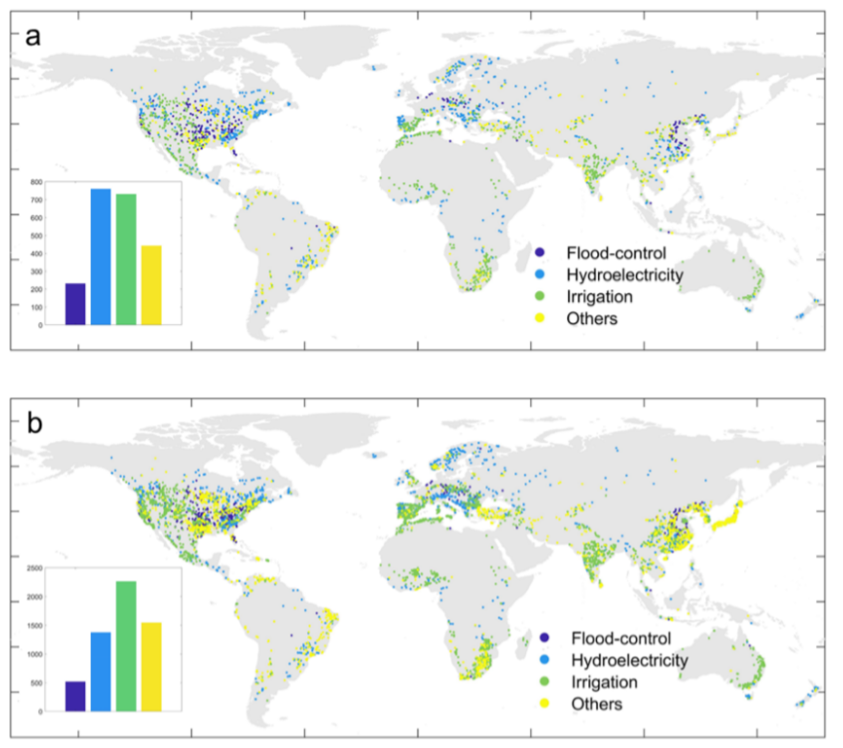
\includegraphics{Figures/陆地表面的水分循环/水库分布.png}
\caption{全球15$'$ (a)和3$'$ (b)河网分辨率下的水库分布。}
\label{fig:水库分布}
\end{figure}
}

水库调度规则参数化方案中所需的水库特征参数包括特征库容 (总库容$V_t$,警戒库容$V_e$、防洪库容$V_f$、
正常库容$V_c$)和特征流量 (防洪流量$Q_f$、正常流量$Q_c$)。
其中,总库容由 GRanD 数据集提供,其他特征库容的提估计需要使用GRSAD \citep{zhao2019towards}和全球水库形状数据集$ReGeo$ \citep{yigzaw2018new} 。
GRSAD提供了GRanD中6817个水库1984年至2015年每月水库面积观测数据的时间序列。
ReGeom提供了GRanD中6824个水库的最佳概化几何形状和对应的蓄水\~面积关系数据。
对于防洪库容$V_f$,定义水库水面达最大面积的75\%时(基于GRSAD数据)水库达到了防洪水位和防洪库容,
将此处的面积对照水库形状数据(基于ReGeom数据)即可得到防洪库容。警戒库容$V_e$和正常库容$V_c$则根据以下公式计算:
\begin{equation}
V_{e}=V_{f}+0.8 \times\left(V_{t}-V_{f}\right)
\end{equation}
\begin{equation}
V_{c}=V_{f} / 2
\end{equation}


如图~\ref{fig:水库特征库容示意图} 所示,水库的特征流量包括防洪流量和正常流量,
防洪流量设定为水库设计洪水流量的50\%,正常流量则设定为坝址处的多年平均日径流量。
坝址处的河道流量数据则是基于CaMa-Flood在自然情景下模拟所得。假设水库设计洪水标准为百年一遇洪水,
基于坝址处模拟的3小时径流量数据,采用Gumbel分布估算重现期为100年的设计洪水\citep{boulange2021}。

{
\begin{figure}[]
\centering
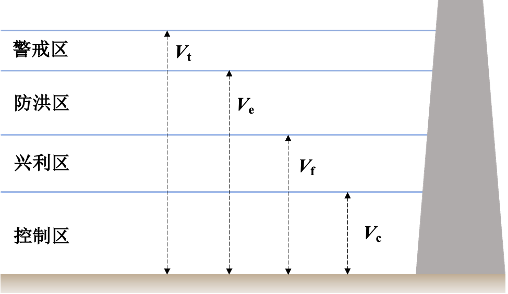
\includegraphics{Figures/陆地表面的水分循环/水库特征库容示意图.png}
\caption{水库特征库容示意图。}
\label{fig:水库特征库容示意图}
\end{figure}
}
\subsection{水库调度规则参数化方案}
在大尺度陆面模式中进行水库扰动模拟,需要对水库的调度规则进行一定的假设和概化,现有方案大致可分为三类:
基于入流和需求的调度方案、基于离线优化的调度方案和基于目标库容的分段调度方案,
其中基于目标库容的方案在高性能 (计算的简单性和透明性) 与全球适用性 (适用场景的代表性和广泛性) 之间能够取得较好的平衡\citep{yassin2019representation}。
因此,本模块的水库调度方案采用基于目标库容的分段调度方式,将水库库容分为四个特征库容区 (如图~\ref{fig:水库特征库容示意图}所示),
不同用途的水库主要区别就在于兴利区和防洪区的调度目标和出流规则。本模块包括了以防洪和需水为目标的水库调度参数化方案。


防洪调度方案根据水库入流量、库容大小和库容调节能力,调节出库流量以削减汛期峰值流量,
控制出库流量不超过防洪流量,且根据汛期发展时段调整出流系数 \citep{hanazaki2022development}:\\
警戒区:
\begin{equation}
Q=\max \left(Q_{f}, I\right)
\end{equation}
防洪区:
\begin{equation}
Q=\begin{cases}
Q_{f}+k \frac{V-V_{f}}{V_{e}-V_{f}}\left(I-Q_{f}\right), & \text{当}\quad I \geq Q_{f} \\
Q_{n} \times 0.5+\left(\frac{V-V_{c}}{V_{e}-V_{c}}\right)^{2}\left(Q_{f}-Q_{n}\right), & \text{当}\quad I<Q_{f}
  \end{cases}
\end{equation}
兴利区:
\begin{equation}
Q=\begin{cases}
Q_{n} \times 0.5+\left(\frac{V-V_{c}}{V_{f}-V_{c}}\right)\left(Q_{f}-Q_{n}\right), & \text{当}\quad I \geq Q_{f} \\
Q_{n} \times 0.5+\left(\frac{V-V_{c}}{V_{e}-V_{c}}\right)^{2}\left(Q_{f}-Q_{n}\right), & \text{当}\quad I<Q_{f}
  \end{cases}
\end{equation}
控制区:
\begin{equation}
Q=Q_{n} \times\left(\frac{V}{V_{f}}\right)
\end{equation}
其中:$I$表示入库流量,$Q$表示出库流量,$V$表示实际库容,$V_e$表示警戒库容,
$V_f$表示防洪库容,$V_c$表示正常库容,$Q_f$表示防洪流量,$Q_n$表示正常流量,$k$表示出流调节系数,
取值为$\max(1-(V_t-V_f)/A,0)$,$A$为水库上游面积,$V_t$为水库总库容。特征库容和特征流量的提取如章节~\ref{水库数据集和水库参数估计} 所述。


需水调度方案则根据水库下游需水量、入库流量、实时库容大小调节出流,以满足水库服务区域内的用水需求 \citep{hanasaki2006reservoir,shin2019high}:\\
警戒区:
\begin{equation}
Q=\max \left(Q_{f}, I\right)
\end{equation}
防洪/兴利区:
\begin{equation}
Q=\begin{cases}
  (1-R) I+R \times \frac{V-V_{c}}{V_{f}-V_{c}} \times\left(Q_{n}+D-\bar{D}\right) & \text{当}\quad
    \bar{D} / Q_{n}<1-M \\ 
  (1-R) I+R \times \frac{V-V_{c}}{V_{f}-V_{c}} \times Q_{n}\left(M+\frac{(1-M) D}{\bar{D}}\right)      &  \text{当}\quad \bar{D} / Q_{n}>M
    \end{cases}
\end{equation}
控制区:
\begin{equation}
Q=Q_{n} \times\left(\frac{V}{V_{f}}\right)
\end{equation}
其中:$\bar{D}̅$表示多年平均日需水量,$D$表示当日需水量,
$M$表示最小需求满足系数 (默认取值为0.5 \citep{hanasaki2006reservoir}),$R$表示需求决定系数,
取值为$\min \left(1, \alpha\left(\frac{V_{f}-V_{d}}{Q_{n}}\right)^{2}\right)$,
$\alpha$为经验参数 (默认取值为4 \citep{hanasaki2006reservoir}),其他变量含义同上式。


\subsection{考虑大坝影响的河道汇流参数化方案}
当水库网格处的蓄水量和水位在水库运行期间增加时,考虑回水影响的模型 (例如CaMa-Flood) 中可能会出现上游回水 (storage buffering effect),
洪水期间河流蓄水量的增加受到水库上游回水的缓冲,将使得模拟入流量波动较小。因此,相比自然河道的汇流方案,考虑大坝影响的汇流方案存在以下改动:
当河道中存在大坝时,由于水的连续流动和河道的水力连结被切断,在与大坝网格紧连的下游网格处,圣维南动力方程中的局部加速项和静水压力项被忽略,
在使用局部惯性方程 (CaMa-Flood中使用的默认算法) 进行一般计算后,使用运动波动方程重新计算流量。
在下一步中,将来自上游河网的所有流出汇总为水库流入,并根据重新计算的流入和蓄水量确定水库流出。
\begin{equation}
g A \frac{\partial z}{\partial x}+\frac{g n^{2}|Q| Q}{R_{H}^{4 / 3} A}=0
\end{equation}
式中变量含义同章节~\ref{诊断洪泛状态} 所述。


此外,由于大坝对汇流过程的拦截作用,在计算大坝网格下游格点的河道蓄水和淹没时,
质量连续方程中的汇流网格和汇流面积将不再包括大坝网格上游的部分,
且与大坝网格紧连的下游网格其入流径流量替换为水库出流量。
\begin{equation}
S_{i}^{t+\Delta t}=S_{i}^{t}+\sum_{k}^{Upstream-2} Q_{k}^{t} \Delta t-Q_{i}^{t} \Delta t+A c_{i} R_{i}^{t} \Delta t
\end{equation}
式中$Upsteam-2$表示在原上游网格的基础上除去大坝上游网格 (例如图~\ref{fig:大坝对下游河道汇流计算方案的影响示意图} 所示),其他变量含义同章节~\ref{诊断洪泛状态} 所述。

{
\begin{figure}[]
\centering
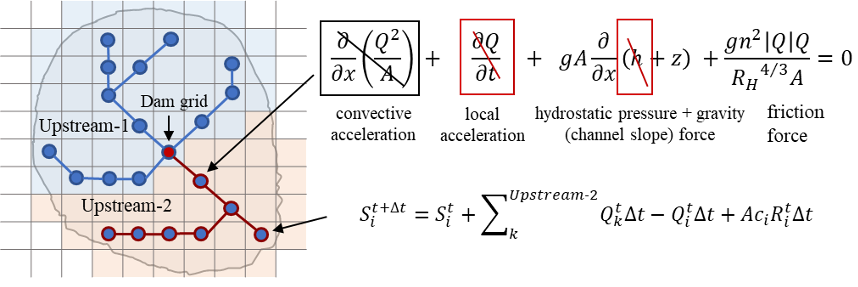
\includegraphics{Figures/陆地表面的水分循环/大坝对下游河道汇流计算方案的影响示意图.png}
\caption{大坝对下游河道汇流计算方案的影响示意图。}
\label{fig:大坝对下游河道汇流计算方案的影响示意图}
\end{figure}
}
\chapter{光合作用和气孔导度}
%\addcontentsline{toc}{chapter}{光合作用和气孔导度}
\begin{mymdframed}{代码}
本节对应的代码文件为\texttt{MOD\_AssimStomataConductance.F90}。
\end{mymdframed}

%\begin{光合作用和气孔导度}

\section{植物的光合作用}\label{植物的光合作用}
CoLM光合作用模型是建立在冠层尺度,双大叶冠层结构基础上的。即冠层尺度的净光合同化速率($A_{\mathrm{n}}$)等于阳叶冠层的净光合同化速率($A_{\mathrm{n,sun}}$)加上阴叶冠层的净光合同化速率($A_{\mathrm{n,sun}}$):
\begin{equation}\label{Ansun_Ansha}
A_{\mathrm{n}}=A_{\mathrm{n,sun}}+A_{\mathrm{n,sha}}
\end{equation}

阳叶和阴叶冠层尺度的净光合同化速率模拟是通过对叶片尺度的光合作用模型进行升尺度而得到。C3植物叶片尺度的光合作用模拟是基于Farquhar光合作用模型~\citep{farquhar1980biochemical},
C4植物则是基于~\citet{collatz1992} 的光合作用改进模型。卡尔文循环是高等植物光合作用中的重要途径之一,CO$_2$和1,5-二磷酸核酮糖(RuBP)在1,5-二磷酸核酮糖羧化酶(Rubisco)的催化下产生羧化反应,生成3-磷酸甘油酸(PGA),并被还原为3-磷酸甘油醛(PGAL),PGA经过一系列转变再次形成RuBP,这被称为RuBP的再生阶段,完成卡尔文循环。当RuBP充足,卡尔文循环稳定时,多余的PGAL才会合成蔗糖和淀粉作为光合作用的产物存储在植物内。Faquhar模型认为卡尔文循环中的Rubisco酶限制($A_{\mathrm{c}}$)和RuBP的再生速率($A_{\mathrm{j}}$)是限制是光合羧化速率的两个关键限制因子,CoLM光合作用模块在此基础上增加了蔗糖和淀粉产物合成的速率限制($A_{\mathrm{p}}$)。另外,叶片净光合同化速率 ($A_{\mathrm{n}}$) 等于总光合同化速率,即三个限制的最小值减去叶呼吸速率 ($R_{\mathrm {d}}$),在阴叶和阳叶冠层分别有:
\begin{equation}\label{An1sun}
A_{\mathrm{n,sun}}=\min \left(A_{\mathrm{c,sun}}, A_{\mathrm{j,sun}}, A_{\mathrm{p,sun}}\right)-R_{\mathrm{d,sun}}
\end{equation}
\begin{equation}\label{An1sha}
A_{\mathrm{n,sha}}=\min \left(A_{\mathrm{c,sha}}, A_{\mathrm{j,sha}}, A_{\mathrm{p,sha}}\right)-R_{\mathrm{d,sha}}
\end{equation}
其中,下标${\mathrm {sun}}$和${\mathrm {sha}}$分别代表在阳叶和阴叶冠层尺度上的光合同化速率和呼吸速率。


RuBP羧化酶限制主要指当羧化酶活性较低时,光合作用羧化速率受限,也称为Rubisco限制。由于Rubisco同时催化RuBP的羧化反应和氧化反应,羧化反应需要CO$_2$而氧化反应需要O$_2$,羧化反应和氧化反应同时进行。因此,C3植物的胞间CO$_2$分压$c_{\mathrm {i}}$和O$_2$分压$o_{\mathrm {i}}$的比例极大影响了Rubisco作为羧化酶的效率。基于这个原因,C3植物的Rubisco限制下的光合同化速率($A_{\mathrm {c}}$)可表达为Michaelis-Menten关于$c_{\mathrm {i}}$和$o_{\mathrm {i}}$的函数。此外,C4植物Rubisco限制下的光合羧化速率不再受胞间CO$_2$分压和O$_2$分压的影响,这是由于C4植物的光合作用途径的最初步骤是磷酸烯醇丙酮酸(PEP)的羧化,PEP羧化酶的活性很高,所以转运到维管束鞘细胞中的CO$_2$的浓度很高,大约是空气中的十倍。C4植物的卡尔文循环在在维管束鞘细胞进行,CO$_2$分压和O$_2$分压的变化对羧化速率的影响较小,因此,Rubisco限制下的光合同化速率在阳叶和阴叶冠层尺度($A_{\mathrm{c,sun}}$和$A_{\mathrm{c,sha}}$)下可表示为胞间CO$_2$分压($c_{\mathrm{i,sun}}$和$c_{\mathrm{i,sha}}$),大气分压($o_{\mathrm{i}}$)和最大羧化速率的函数($V_{\mathrm{cmax,sun}}$和$V_{\mathrm{cmax,sha}}$):
\begin{equation}\label{A_C1sun}
A_{\mathrm{c,sun}}=\begin{cases}
\frac{V_{\mathrm{cmax,sun}}\left(c_{\mathrm{i,sun}}-\Gamma_{\mathrm{sun}}\right)}{c_{\mathrm{i,sun}}+K_{\mathrm{c}}\left(1+\frac{o_{\mathrm{i}}}{K_{\mathrm{o}}}\right)}
     & \text{for C3 plants} \\
V_{\mathrm{cmax,sun }} & \text{for C4 plants}
\end{cases}
\end{equation}
\begin{equation}\label{A_C1sha}
A_{\mathrm{c,sha}}=\begin{cases}
\frac{V_{\mathrm{cmax,sha}}\left(c_{\mathrm{i,sha}}-\Gamma_{\mathrm{sha}}\right)}{c_{\mathrm{i,sha}}+K_{\mathrm{c}}\left(1+\frac{o_{\mathrm{i}}}{K_{\mathrm{o}}}\right)}
     & \text{for C3 plants} \\
V_{\mathrm{cmax,sha }} & \text{for C4 plants}
\end{cases}
\end{equation}

其中,下标${\mathrm {sun}}$和${\mathrm {sha}}$分别代表在阳叶和阴叶冠层尺度上的相应变量,$\Gamma$是CO$_2$补偿点,单位为:Pa,$K_{\mathrm {c}}$和$K_{\mathrm {o}}$分别是对于CO$_2$和O$_2$的Michaelis--Menten常数(Pa),$V_{\mathrm{cmax,sun}}$和$V_{\mathrm{cmax,sha}}$代表阳叶和阴叶冠层尺度的最大羧化速率,它是根据叶面积指数从叶片尺度上升到冠层尺度的光合参数。

C3植物:
\begin{equation}\label{V_cmaxsun_a}
V_{\mathrm{cmax,sun }}=\frac{V_{\mathrm{cmax 25}} \cdot 2.1^{\frac{T_{\mathrm{{leaf }}}-T_{\mathrm{o p}}}{10}}}{1+{\mathrm e}^{s_{\mathrm{1}}\left(T_{\mathrm{{leaf }}}-T_{\mathrm{{high }}}\right)}} \cdot \beta_{\mathrm{sun}} \cdot L_{\mathrm{v,sun}}
\end{equation}
\begin{equation}\label{V_cmaxsha_a}
V_{\mathrm{cmax,sha }}=\frac{V_{\mathrm{cmax 25}} \cdot 2.1^{\frac{T_{\mathrm{{leaf }}}-T_{\mathrm{o p}}}{10}}}{1+{\mathrm e}^{s_{\mathrm{1}}\left(T_{\mathrm{{leaf }}}-T_{\mathrm{{high }}}\right)}} \cdot \beta_{\mathrm{sha}} \cdot L_{\mathrm{v,sha}}
\end{equation}

C4植物:
\begin{equation}\label{V_cmaxsun_b}
V_{\mathrm{cmax,sun }}= \frac{V_{\mathrm{cmax 25}} \cdot 2.1^{\frac{T_{\mathrm{{leaf }}}-T_{\mathrm{o p}}}{10}}}{\left(1+{\mathrm e}^{s_{\mathrm{2}}\left(T_{\mathrm{{low }}}
 - T_{\mathrm{{leaf }}}\right)}\right)\left(1+{\mathrm e}^{s_{\mathrm{1}}\left(T_{\mathrm{{leaf }}}-T_{\mathrm{h i g h}}\right)}\right)} \cdot \beta_{\mathrm{sun}} \cdot L_{\mathrm{v,sun}}
\end{equation}
\begin{equation}\label{V_cmaxsha_b}
V_{\mathrm{cmax,sha }}= \frac{V_{\mathrm{cmax 25}} \cdot 2.1^{\frac{T_{\mathrm{{leaf }}}-T_{\mathrm{o p}}}{10}}}{\left(1+{\mathrm e}^{s_{\mathrm{2}}\left(T_{\mathrm{{low }}}
 - T_{\mathrm{{leaf }}}\right)}\right)\left(1+{\mathrm e}^{s_{\mathrm{1}}\left(T_{\mathrm{{leaf }}}-T_{\mathrm{h i g h}}\right)}\right)} \cdot \beta_{\mathrm{sha}} \cdot L_{\mathrm{v,sha}}
\end{equation}
不同植被的羧化能力存在差异,我们用25 \textcelsius 下的最大羧化速率 $V_{\mathrm{cmax 25}}$ 来刻画植被的光合羧化能力,单位: \unit{mol.m^{-2}.s^{-1}};Rubisco羧化酶的活性随温度显著变化,CoLM光合作用模块针对C3和C4植物制定了两套温度响应函数。$T_{\mathrm{op}}$是参考温度298 K;$s_1$和$s_2$分别为高温和低温的温度敏感性参数;$T_{\mathrm{low}}$和$T_{\mathrm{high}}$分别为羧化速率的低温和高温响应参数,
取值根据植被类型而变化,范围分别为: 278$\sim$288 K,303$\sim$313 K;$T_{\mathrm{leaf}}$是叶片温度,通过对叶片能量平衡方程进行牛顿迭代方法而求解得到,详见章节~\ref{植被叶片温度计算},$\beta_{\mathrm{sun}}$和$\beta_{\mathrm{sha}}$是阳叶和阴叶的水分胁迫因子,水分胁迫因子的取值范围0$\sim$1,详见章节~\ref{气孔导度的水分胁迫}。当植被水力模式开启时,需要最大气孔导度作为植被水力模式输入,在水分胁迫因子为1的条件下,光合气孔耦合模型可得到最大气孔导度。另外,$L$代表叶片到冠层的尺度转换系数,下标sun和sha分别代表阳叶和阴叶,$v$代表参数$V_{\mathrm{cmax}}$的转换系数,它们均是叶面积指数的函数:
%
\begin{equation}\label{L_vsun}
L_{\mathrm{v,sun}}=\frac{1-{\mathrm e}^{-\left(0.11+K_{\mathrm{b}}\right) \cdot {\rm LAI}}}{0.11+K_{\mathrm{b}}}
\end{equation}
\begin{equation}\label{L_vsha}
L_{\mathrm{v,sha}}=\frac{1-{\mathrm e}^{-0.11\cdot {\rm LAI}}}{0.11} - L_{\mathrm{v,sun}}
\end{equation}
$K_{\mathrm{b}}$代表直射光的消光系数。

当光照不足时,RuBP再生速率下降,成为制约光合作用开尔文循环的最主要因素。因此,RuBP再生速率限制下的羧化速率在阳叶和阴叶冠层尺度下 ($A_{\mathrm{j,sun}}$和$A_{\mathrm{j,sha}}$) 可表达为阳叶和阴叶的有效光合辐射 (${\rm PAR}_{\mathrm{sun}}$和${\rm PAR}_{\mathrm{sha}}$) 的函数:
\begin{equation}\label{A_J1sun}
A_{\mathrm{j,sun}}=\begin{cases}\frac{J_{\mathrm{x,sun}}\cdot\left(c_{\mathrm{i,sun}}-\Gamma\right)}{c_{\mathrm{i,sun}}+2\Gamma}
     & \text{for C3 plants} \\
J_{\mathrm{x,sun}} & \text{for C4 plants}
\end{cases}
\end{equation}
\begin{equation}\label{A_J1sha}
A_{\mathrm{j,sha}}=\begin{cases}\frac{J_{\mathrm{x,sha}}\cdot\left(c_{\mathrm{i,sha}}-\Gamma\right)}{c_{\mathrm{i,sha}}+2\Gamma}
     & \text{for C3 plants} \\
J_{\mathrm{x,sha}} & \text{for C4 plants}
\end{cases}
\end{equation}

$J_{\mathrm{x,sun}}$和$J_{\mathrm{x,sha}}$是阳叶和阴叶冠层尺度的电子传输速率,是有效光合辐射(${\rm PAR}_{\mathrm{sun}}$和${\rm PAR}_{\mathrm{sha}}$)的函数,并受叶片温度 ($T_{\mathrm{leaf}}$)和水分胁迫因子($\beta_{\mathrm{sun}}$和$\beta_{\mathrm{sha}}$)的调节:
\begin{equation}
\begin{aligned}
J_{\mathrm{x,sun}}=\min \left(\begin{array}{c} \alpha\left(4.6 \times 10^{-6} \cdot {\rm PAR}_{\mathrm{sun}}\right), \\
  J_{\mathrm{x25}} \cdot \exp\left(\frac{37000\left(T_{\mathrm{{leaf }}}-T_{\mathrm{o p}}\right)}{T_{\mathrm{o p}} \cdot T_{\mathrm{{leaf }}} \cdot {\rm R} } \right ) \cdot\frac{1+\exp\left(\frac{710 \cdot T_{\mathrm{o p}}-220000} {{\rm R} \cdot T_{\mathrm{o p}}}\right)}  {1+\exp\left(\frac{710 \cdot T_{\mathrm{leaf}}-220000} {{\rm R} \cdot T_{\mathrm{{leaf}}}}\right)} \cdot \beta_{\mathrm{sun}} \cdot L_{\mathrm{j,sun}}  \end{array} \right)
\end{aligned}
\end{equation}
\begin{equation}
\begin{aligned}
J_{\mathrm{x,sha}}=\min \left(\begin{array}{c} \alpha\left(4.6 \times 10^{-6} \cdot {\rm PAR}_{\mathrm{sha}}\right), \\
  J_{\mathrm{x25}} \cdot \exp\left(\frac{37000\left(T_{\mathrm{{leaf }}}-T_{\mathrm{o p}}\right)}{T_{\mathrm{o p}} \cdot T_{\mathrm{{leaf }}} \cdot {\rm R} } \right ) \cdot\frac{1+\exp\left(\frac{710 \cdot T_{\mathrm{o p}}-220000} {{\rm R} \cdot T_{\mathrm{o p}}}\right)}  {1+\exp\left(\frac{710 \cdot T_{\mathrm{leaf}}-220000} {{\rm R} \cdot T_{\mathrm{{leaf}}}}\right)} \cdot \beta_{\mathrm{sha}} \cdot L_{\mathrm{j,sha}}  \end{array} \right)
\end{aligned}
\end{equation}
其中$\alpha$是量子效率 (C3植被设置为0.08,C4植被为0.05,单位为\unit{mol.CO_2.mol^{-1}.photon});${\mathrm {PAR}}$是有效光合辐射,单位: \unit{W.m^{-2}},详细计算见章节~\ref{短波吸收辐射通量};
\num{4.6e-6} 代表单位从 \unit{W.m^{-2}} 转换到 \unit{mol.photon.m^{-2}} 的转换系数;
$J_{\mathrm{x25}}$是25 \textcelsius 下的最大电子传输速率,单位: \unit{mol.m^{-2}.s^{-1}},$J_{\mathrm{x25}}=1.97 \cdot V_{\mathrm{cmax 25}}$;
R是通用气体常数,${\rm R}=$ \qty{8.3145}{mol.m^{-2}.s^{-1}}。$L_{\mathrm{j,sun}}$和$L_{\mathrm{j,sha}}$代表电子传输速率的尺度转换系数(叶片到冠层):
%
\begin{equation}\label{L_jsun}
L_{\mathrm{j,sun}}=\frac{1-{\mathrm e}^{-\left(K_{\mathrm{d}}+K_{\mathrm{b}}\right) \cdot {\rm LAI}}}{K_{\mathrm{d}}+K_{\mathrm{b}}}
\end{equation}
\begin{equation}\label{L_jsha}
L_{\mathrm{j,sha}}=\frac{1-{\mathrm e}^{-K_{\mathrm{d}}\cdot {\rm LAI}}}{K_{\mathrm{d}}} - L_{\mathrm{j,sun}}
\end{equation}
$K_{\mathrm{d}}$代表散射光的消光系数。

第三,光合作用速率还受到卡尔文循环中蔗糖和淀粉的合成速率限制($A_{\mathrm{p,sun}}$和$A_{\mathrm{p,sha}}$),在阳叶和阴叶冠层尺度上,用冠层25 \textcelsius 最大羧化速率 ($V_{\mathrm{cmax25}}$) 进行参数化,并且描述其受叶温和水分胁迫因子的调控:

C3植物:
\begin{equation}\label{A_e_a_sun}
A_{\mathrm{p,sun}}=\frac{V_{\mathrm{cmax 25}}}{2} \cdot \frac{1.8^{\frac{T_{\mathrm{{leaf }}}-T_{\mathrm{o p}}}{10}}}{1+{\mathrm e}^{s_{\mathrm{2}}\left(T_{\mathrm{{low }}}-T_{\mathrm{{leaf }}}\right)}} \cdot \beta_{\mathrm{sun}} \cdot L_{\mathrm{v,sun}}
\end{equation}
\begin{equation}\label{A_e_a_sha}
A_{\mathrm{p,sha}}=\frac{V_{\mathrm{cmax 25}}}{2} \cdot \frac{1.8^{\frac{T_{\mathrm{{leaf }}}-T_{\mathrm{o p}}}{10}}}{1+{\mathrm e}^{s_{\mathrm{2}}\left(T_{\mathrm{{low }}}-T_{\mathrm{{leaf }}}\right)}} \cdot \beta_{\mathrm{sha}} \cdot L_{\mathrm{v,sha}}
\end{equation}

C4植物:
\begin{equation}\label{A_e_b_sun}
A_{\mathrm{p,sun}}=a_{\mathrm{p}} \cdot V_{\mathrm{cmax 25}} \cdot 1.8^{\frac{T_{\mathrm{{leaf }}}-T_{\mathrm{op}}}{10}} \cdot c_{\mathrm{i,sun}}/p_{\mathrm{s}} \cdot \beta_{\mathrm{sun}} \cdot L_{\mathrm{v,sun}}
\end{equation}
\begin{equation}\label{A_e_b_sha}
A_{\mathrm{p,sha}}=a_{\mathrm{p}} \cdot V_{\mathrm{cmax 25}} \cdot 1.8^{\frac{T_{\mathrm{{leaf }}}-T_{\mathrm{op}}}{10}} \cdot c_{\mathrm{i,sha}}/p_{\mathrm{s}} \cdot \beta_{\mathrm{sha}} \cdot L_{\mathrm{v,sha}}
\end{equation}
$a_{\mathrm{p}}$是产物合成速率的无量纲经验系数,取值$2\times10^4$,$a_{\mathrm{p}}/p_{\mathrm{s}}\approx 0.2$ Pa$^{-1}$。三方面限制下的光合同化速率共用同一套温度响应常数 ($T_{\mathrm{op}}$,$T_{\mathrm{low}}$和$T_{\mathrm{high}}$)以及温度敏感性参数($s_1$和$s_2$)。


阳叶和阴叶冠层尺度的呼吸速率($R_{\mathrm{d,sun}}$和$R_{\mathrm{d,sha}}$)对温度的响应曲线可表示为$V_{\mathrm{cmax25}}$的函数:
\begin{equation}\label{R_d1_sun}
R_{\mathrm{d,sun}}=\tau_{\mathrm{{base }}} \cdot V_{\mathrm{cmax 25}} \cdot \frac{2.0^{\frac{T_{\mathrm{leaf}}-T_{\mathrm{op}}}{10}}}{1+{\mathrm e}^{1.3 \cdot\left(T_{\mathrm{leaf}}-T_{\mathrm{d m}}\right)}} \cdot \beta_{\mathrm{sun}} \cdot L_{\mathrm{v,sun}}
\end{equation}
\begin{equation}\label{R_d1_sha}
R_{\mathrm{d,sha}}=\tau_{\mathrm{{base }}} \cdot V_{\mathrm{cmax 25}} \cdot \frac{2.0^{\frac{T_{\mathrm{leaf}}-T_{\mathrm{op}}}{10}}}{1+{\mathrm e}^{1.3 \cdot\left(T_{\mathrm{leaf}}-T_{\mathrm{d m}}\right)}} \cdot \beta_{\mathrm{sha}} \cdot L_{\mathrm{v,sha}}
\end{equation}
其中$T_{\mathrm{dm}}$是叶呼吸的高温抑制温度常数,单位 K; $\tau_{\mathrm{base}}$是基础呼吸速率系数,无量纲。

在方程\eqref{An1sun}和\eqref{An1sha}求解最小值的计算中,我们将三值最小问题的求解拆分为两个二值最小问题的求解:
\begin{equation}\label{min_Ac_Aj_Ae}
\min \left(A_{\mathrm{c}}, A_{\mathrm{j}}, A_{\mathrm{p}}\right)
= \min \left[\min \left(A_{\mathrm{c}}, A_{\mathrm{j}}\right), A_{\mathrm{p}}\right]
\end{equation}
引入形状参数$\theta$,构造一元二次方程,将求解最小值问题转换成求一元二次方程较小根的问题,以此避免模拟中不同光合限制之间过渡转换时的光合同化速率突变~\citep{collatz1991,collatz1992}:
\begin{equation}\label{theta_cj}
\theta_{\mathrm{c j}} \cdot A_{\mathrm{i1}}^{2}-\left(A_{\mathrm{c}}+A_{\mathrm{j}}\right) A_{\mathrm{i1}}+A_{\mathrm{c}} A_{\mathrm{j}}=0
\end{equation}
\begin{equation}\label{theta_cjp}
\theta_{\mathrm{c j p}} \cdot A_{\mathrm{i2}}^{2}-\left(A_{\mathrm{i1}}+A_{\mathrm{p}}\right) A_{\mathrm{i2}}+A_{\mathrm{i1}} A_{\mathrm{p}}=0
\end{equation}
其中形状参数$\theta_{\mathrm{cj}}=0.877$,$\theta_{\mathrm{cjp}}=0.95$。$A_{\mathrm{i1}}$为方程\eqref{theta_cj}的较小根,代表$A_{\mathrm {c}}$和$A_{\mathrm {j}}$的最小值。$A_{\mathrm{i2}}$为方程\eqref{theta_cjp}的较小根,代表$A_{\mathrm{i1}}$和$A_{\mathrm {p}}$的最小值。


\section{气体扩散方程和气孔导度模型}\label{气体扩散方程和气孔导度模型}
气孔是植被和大气相互作用的最重要通道,陆地生态系统碳水耦合很大程度取决于气孔的行为。CoLM在净光合同化速率和蒸腾速率计算中,考虑植被气孔的行为,结合气体扩散方程,刻画了碳水通量与浓度梯度之间的重要关系。

\subsection{气体扩散方程}

CoLM将CO$_2$和水汽的气体扩散问题类比于电路问题进行建模,利用叶绿体细胞间、叶表和冠层大气的$\rm CO_2$浓度和水汽浓度梯度,来刻画环境对植被碳水通量的驱动力~\eqref{A_n2_sun}--~\eqref{ea_ei_sha},如图~\ref{fig:叶片气孔光合作用导度模型示意图} 所示。
%
{
\begin{figure}[htbp]
\centering
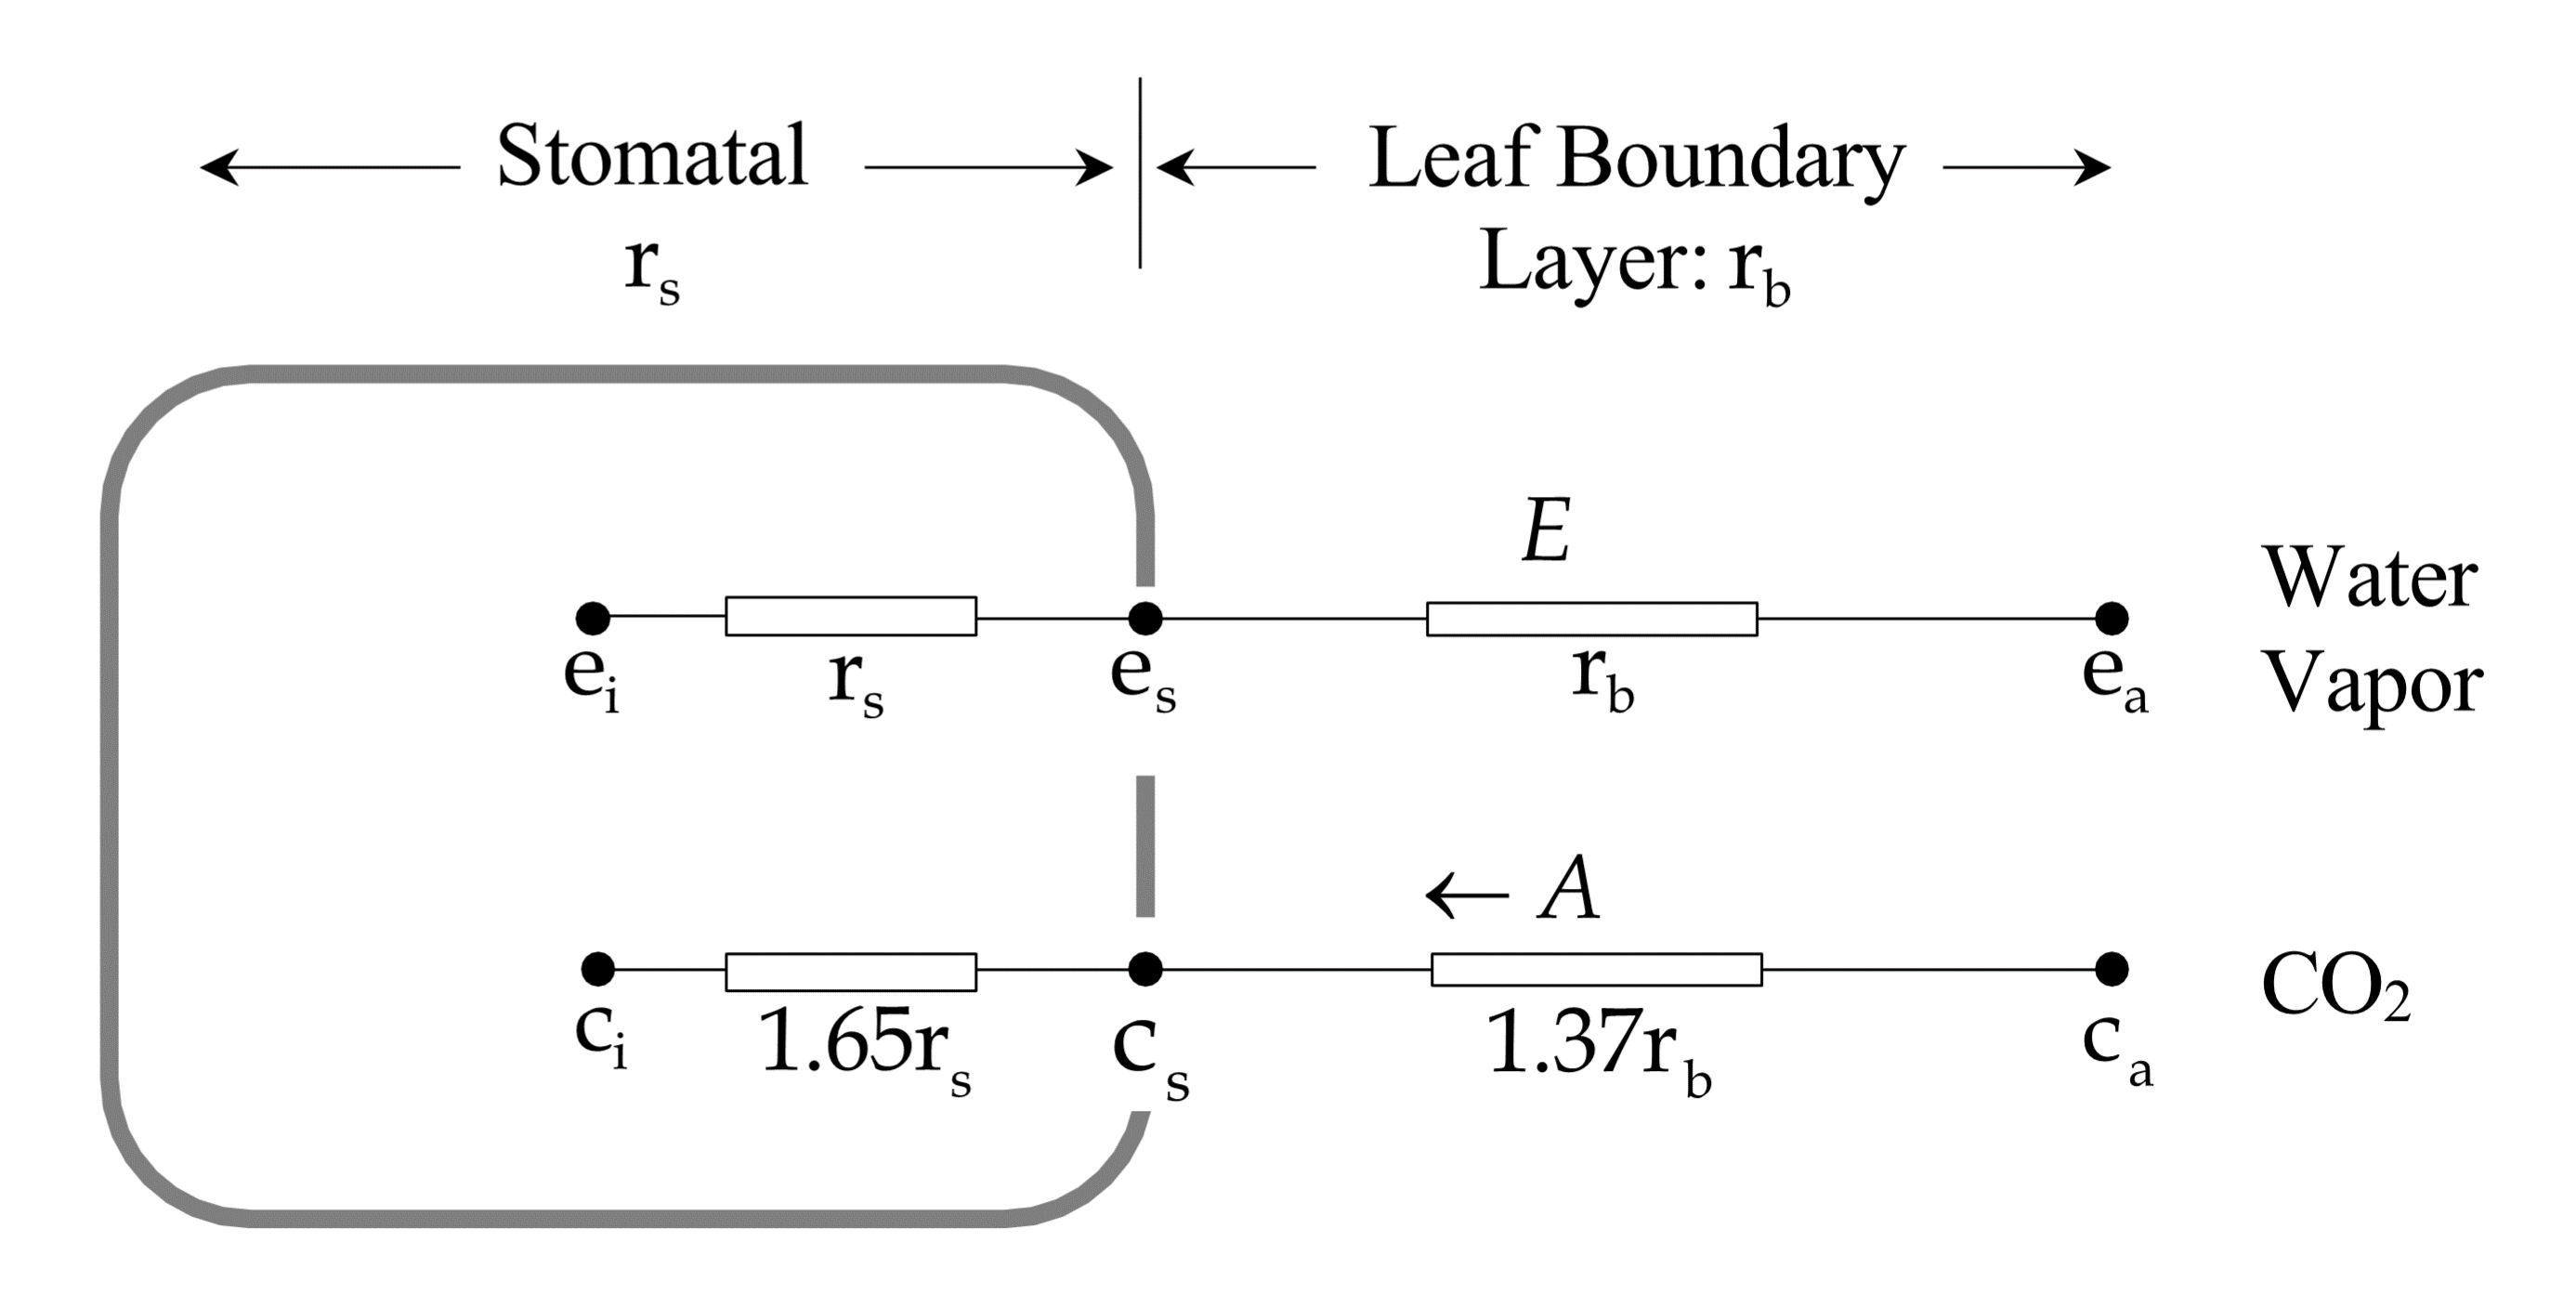
\includegraphics[width=0.8\textwidth]{Figures/气孔导度和光合作用/叶片气孔光合作用导度模型示意图.png}
\caption{叶片气孔光合作用导度模型示意图}
\label{fig:叶片气孔光合作用导度模型示意图}
\end{figure}
}

在阳叶和阴叶冠层尺度上,分别存在关于$\rm CO_2$和水汽的气体扩散方程:
\begin{equation}\label{A_n2_sun}
A_{\mathrm{n,sun}}=\left(\frac{c_{\mathrm{a}}-c_{\mathrm{i,sun}}}{p_{\mathrm{s}}}\right) /\left(\frac{1.37}{G_{\mathrm{b}}} +\frac{1.6}{G_{\mathrm{s,sun}}}\right)=\left(\frac{c_{\mathrm{s,sun}}-c_{\mathrm{i,sun}}}{p_{\mathrm{s}}}\right) /\left(\frac{1.6}{G_{\mathrm{s,sun}}}\right)
\end{equation}
\begin{equation}\label{A_n2_sha}
A_{\mathrm{n,sha}}=\left(\frac{c_{\mathrm{a}}-c_{\mathrm{i,sha}}}{p_{\mathrm{s}}}\right) /\left(\frac{1.37}{G_{\mathrm{b}}} +\frac{1.6}{G_{\mathrm{s,sha}}}\right)=\left(\frac{c_{\mathrm{s,sha}}-c_{\mathrm{i,sha}}}{p_{\mathrm{s}}}\right) /\left(\frac{1.6}{G_{\mathrm{s,sha}}}\right)
\end{equation}
\begin{equation}\label{ea_ei_sun}
E_{\mathrm{v,sun}}=\left(\frac{e_{\mathrm{a}}-e_{\mathrm{i}}}{p_{\mathrm{s}}}\right) /\left(\frac{1}{G_{\mathrm{b}}}+\frac{1}{G_{\mathrm{s,sun}}}\right)=\left(\frac{e_{\mathrm{s,sun}}-e_{\mathrm{i}}}{p_{\mathrm{s}}}\right) / \frac{1}{G_{\mathrm{s,sun}}}
\end{equation}
\begin{equation}\label{ea_ei_sha}
E_{\mathrm{v,sha}}=\left(\frac{e_{\mathrm{a}}-e_{\mathrm{i}}}{p_{\mathrm{s}}}\right) /\left(\frac{1}{G_{\mathrm{b}}}+\frac{1}{G_{\mathrm{s,sha}}}\right)=\left(\frac{e_{\mathrm{s,sha}}-e_{\mathrm{i}}}{p_{\mathrm{s}}}\right) / \frac{1}{G_{\mathrm{s,sha}}}
\end{equation}
其中,$c_{\mathrm{i,sun}}$和$c_{\mathrm{i,sha}}$是阳叶和阴叶的胞间CO$_2$分压,$c_{\mathrm{s,sun}}$和$c_{\mathrm{s,sha}}$是阳叶和阴叶的叶表CO$_2$分压,$c_{\mathrm {a}}$是冠层大气$\rm CO_2$分压,单位: Pa;$e_{\mathrm{s,sun}}$和$e_{\mathrm{s,sha}}$是阳叶和阴叶的叶表水汽分压,$e_{\mathrm {a}}$是冠层大气水汽分压,$e_{\mathrm {i}}$是胞间水汽分压,单位: Pa,通常假定为饱和水汽压,$G_{\mathrm {b}}$是冠层尺度的叶边界层导度,$G_{\mathrm{s,sun}}$和$G_{\mathrm{s,sha}}$是阳叶和阴叶的冠层尺度叶气孔导度,单位: \unit{mol.m^{-2}.s^{-1}}。

气孔导度理论认为植被根据自身光合同化速率、环境大气水分亏缺以及土壤水分胁迫等因素,主动调控气孔导度。CoLM的气孔导度模型包含最优气孔导度模型和经验气孔导度模型两个选择,默认情况下对C3植被采用基于最优水分利用效率理论的WUE最优气孔导度模型~\citep{Liang2023},对C4植物仍采用传统的Ball-Berry经验气孔导度模型。

\subsection{WUE最优气孔导度模型}

最优气孔导度模型假设在无水分胁迫的条件下,气孔总会自我调节使得水分利用效率最大,如果净光合同化速率($ A_{\mathrm{n,sun}}$和$ A_{\mathrm{n,sha}}$)和蒸腾($ E_{\mathrm{v,sun}}$和$ E_{\mathrm{v,sha}}$)都被视为气孔导度的函数,水分利用效率($ A_{\mathrm{n,sun}}/E_{\mathrm{v,sun}}$和$ A_{\mathrm{n,sha}}/E_{\mathrm{v,sha}}$)能够取到极值的条件是,净光合同化速率和蒸腾对气孔导度($ G_{\mathrm{s,sun}}$和$ G_{\mathrm{s,sha}}$)偏微分为常数:
\begin{equation}\label{lambda_sun}
\lambda_{\mathrm{sun}}=\frac{\mathrm{d} E_{\mathrm{v,sun}}/\mathrm{d} G_{\mathrm{s,sun}}}{\mathrm{d} A_{\mathrm{n,sun}}/\mathrm{d} G_{\mathrm{s,sun}}}
\end{equation}
\begin{equation}\label{lambda_sha}
\lambda_{\mathrm{sha}}=\frac{\mathrm{d} E_{\mathrm{v,sha}}/\mathrm{d} G_{\mathrm{s,sha}}}{\mathrm{d} A_{\mathrm{n,sha}}/\mathrm{d} G_{\mathrm{s,sha}}}
\end{equation}

我们将常数$\lambda_{\mathrm{sun}}$和$\lambda_{\mathrm{sha}}$分别称为阳叶和阴叶的边际水分利用成本,根据扩散方程~\eqref{A_n2_sun}--~\eqref{ea_ei_sha},边际水分利用效率的计算可以进一步展开,由于阳叶和阴叶的计算方式相同,我们将它的计算合并为一组公式,同时代表阳叶和阴叶的计算,在蒸腾偏微分的计算中~\eqref{dEdgs},我们忽略了叶片边界层导度:
\begin{equation}\label{dEdgs}
\frac{\mathrm{d} E_{\mathrm{v}}}{\mathrm{d} G_{\mathrm{s}}}=\frac{e_{\mathrm{i}}-e_{\mathrm{a}}}{p_{\mathrm{s}}}
\end{equation}

在净光合同化速率偏微分的计算中,气孔导度$G_{\mathrm{s}}$是通过影响胞间$\mathrm {CO_2}$分压,来控制净光合同化速率$A_{\mathrm{n}}$,净光合同化速率是胞间$\rm CO_2$分压$c_{\mathrm{i}}$的函数,胞间$\mathrm {CO_2}$分压$c_{\mathrm{i}}$是气孔导度的函数。因此,对净光合同化速率偏微分的计算需要利用复函数求导法则:
\begin{equation}\label{dAdgs1}
\frac{\mathrm{d} A_{\mathrm{n}}\left(c_{\mathrm{i}}\left(G_{\mathrm{s}}\right)\right)}{\mathrm{d} G_{\mathrm{s}}}= \frac{\mathrm{d} A_{\mathrm{n}}}{\mathrm{d} c_{\mathrm{i}}}\frac{\mathrm{d} c_{\mathrm{i}}}{\mathrm{d} G_{\mathrm{s}}}
\end{equation}

当我们忽略叶片边界层导度,扩散方程~\eqref{A_n2_sun}和~\eqref{A_n2_sha}可以被看成胞间$\mathrm {CO_2}$分压$c_{\mathrm{i}}$关于气孔导度$G_{\mathrm{s}}$的隐函数:
\begin{equation}\label{cigsimplicit}
F\left(G_{\mathrm{s}},c_{\mathrm{i}}\right)=1.6p_{\mathrm{s}}A_{\mathrm{n}}\left(c_{\mathrm{i}}\right)-\left(c_{\mathrm{a}}-c_{\mathrm{i}}\right) G_{\mathrm{s}}=0
\end{equation}

隐函数$F\left(G_{\mathrm{s}},c_{\mathrm{i}}\right)$对气孔导度$G_{\mathrm{s}}$求导,结合气体扩散方程~\eqref{A_n2_sun}和~\eqref{A_n2_sha},并忽略叶片边界层导度可得:
\begin{equation}\label{dcidgs}
    \frac{\mathrm{d}c_{\mathrm{i}}}{\mathrm{d}G_{\mathrm{s}}}=\frac{c_{\mathrm{a}}-c_{\mathrm{i}}}{1.6p_{\mathrm{s}}\frac{\mathrm{d}A_{\mathrm{n}}}{\mathrm{d}c_{\mathrm{i}}}+G_{\mathrm{s}}}=\frac{c_{\mathrm{a}}-c_{\mathrm{i}}}{1.6p_{\mathrm{s}}\frac{\mathrm{d}A_{\mathrm{n}}}{\mathrm{d}c_{\mathrm{i}}}+1.6p_{\mathrm{s}}\frac{A_{\mathrm{n}}}{c_{\mathrm{a}}-c_{\mathrm{i}}}}
\end{equation}

把~\eqref{dcidgs} 代入~\eqref{dAdgs1} 得到:
\begin{equation}\label{dAdgs2}
    \frac{\mathrm{d}A_{\mathrm{n}}}{\mathrm{d}G_{\mathrm{s}}}=\frac{\left(c_{\mathrm{a}}-c_{\mathrm{i}}\right)^2}{1.6p_{\mathrm{s}}\left(c_{\mathrm{a}}-c_{\mathrm{i}}+\frac{A_{\mathrm{n}}}{\frac{\mathrm{d}A_{\mathrm{n}}}{\mathrm{d}c_{\mathrm{i}}}}\right)}
\end{equation}

把~\eqref{dAdgs2} 和~\eqref{dEdgs} 代入~\eqref{lambda_sun} 和~\eqref{lambda_sha},得到边际水分利用成本的计算公式:
\begin{equation}\label{lambda}
\lambda=\frac{1.6\left(e_{\mathrm{i}}-e_{\mathrm{a}}\right)\left(c_{\mathrm{a}}-c_{\mathrm{i}}+\frac{A_{\mathrm{n}}}{\frac{\mathrm{d}A_{\mathrm{n}}}{\mathrm{d}c_{\mathrm{i}}}}\right)}{\left(c_{\mathrm{a}}-c_{\mathrm{i}}\right)^2}
\end{equation}

假设光合同化速率受只受Rubisco酶和RuBP再生速率的限制,且忽略叶呼吸速率$R_{\mathrm{d}}$即$A_{\mathrm{n}}=\mathrm{min}\left(A_{\mathrm{c}},A_{\mathrm{j}}\right)$, 公式~\eqref{lambda} 中关于光合同化速率这一项 $\frac{A_{\mathrm{n}}}{\frac{\mathrm{d}A_{\mathrm{n}}}{\mathrm{d}c_{\mathrm{i}}}}$可以通过求~\eqref{A_C1sun}、\eqref{A_C1sha}、\eqref{A_J1sun} 和~\eqref{A_J1sha} 关于$c_{\mathrm{i}}$的导数得到:
%
\begin{equation}\label{AdAdci}
    \frac{A_{\mathrm{n}}}{\frac{\mathrm{d}A_{\mathrm{n}}}{\mathrm{d}c_{\mathrm{i}}}}=\min\left\{\frac{\left[c_{\mathrm{i}}+K_{\mathrm{c}}\left(1+\frac{o_{\mathrm{i}}}{K_{\mathrm{o}}}\right)\right]\left(c_{\mathrm{i}}-\Gamma^*\right)}{\Gamma^*+K_{\mathrm{c}}\left(1+\frac{o_{\mathrm{i}}}{K_{\mathrm{o}}}\right)},\frac{\left(c_{\mathrm{i}}+2\Gamma^*\right)\left(c_{\mathrm{i}}-\Gamma^*\right)}{3\Gamma^*}\right\}
\end{equation}

将~\eqref{AdAdci} 代入边际水分利用成本计算公式~\eqref{lambda} 进一步展开:
\begin{equation}\label{cieqn}
\begin{cases}
    \left(c_{\mathrm{a}}-c_{\mathrm{i}}\right)^2-\frac{1.6\left(e_{\mathrm{i}}-e_{\mathrm{a}}\right)}{\lambda}\left(\frac{\left(c_{\mathrm{i}}+K_{\mathrm{c}}\left(1+\frac{o_{\mathrm{i}}}{K_{\mathrm{o}}}\right)\right)\left(c_i-\Gamma^*\right)}{\Gamma^*+K_{\mathrm{c}}\left(1+\frac{o_{\mathrm{i}}}{K_{\mathrm{o}}}\right)}+c_{\mathrm{a}}-c_{\mathrm{i}}\right)=0 & \text{Rubisco限制}  \\
    \left(c_{\mathrm{a}}-c_{\mathrm{i}}\right)^2-\frac{1.6\left(e_{\mathrm{i}}-e_{\mathrm{a}}\right)}{\lambda}\left(\frac{\left(c_{\mathrm{i}}+2\Gamma^*\right)\left(c_i-\Gamma^*\right)}{3\Gamma^*}+c_{\mathrm{a}}-c_{\mathrm{i}}\right)=0  & \text{RuBP再生限制}
\end{cases}
\end{equation}

假设胞间$\mathrm {CO_2}$分压远远小于Michaelis-Menten常数,即$c_{\mathrm{i}}\ll K_{\mathrm{c}}\left(1+\frac{o_{\mathrm{i}}}{K_{\mathrm{o}}}\right)$;大气$\mathrm {CO_2}$分压远大于补偿点分压,即$c_{\mathrm{a}}\gg\Gamma^*$;$\frac{1.6\left(e_{\mathrm{i}}-e_{\mathrm{a}}\right)}{\lambda}$不远小于1,即$c_{\mathrm{a}}\gg\frac{1.6\left(e_{\mathrm{i}}-e_{\mathrm{a}}\right)\Gamma^*}{\lambda}$,可以从~\eqref{cieqn}中解出胞间$\mathrm {CO_2}$分压$c_{\mathrm{i}}$:

\begin{equation}\label{cisolu}
    \begin{cases}
    c_{\mathrm{i}}=c_{\mathrm{a}} - \sqrt{\frac{1.6\left(e_{\mathrm{i}}-e_{\mathrm{a}}\right)\left(c_{\mathrm{a}}-\Gamma^*\right)}{\lambda}} \\
    c_{\mathrm{i}}=c_{\mathrm{a}} - \frac{c_{\mathrm{a}}}{1+1.37\sqrt{\frac{\lambda \Gamma^*}{e_{\mathrm{i}}-e_{\mathrm{a}}}}}
    \end{cases}
\end{equation}

将胞间$\mathrm {CO_2}$分压~\eqref{R_d1_sha}代入光合作用模块~\eqref{An1sun}-~\eqref{R_d1_sha},即可计算光合同化速率$A_{\mathrm{n,sun}}$和$A_{\mathrm{n,sha}}$。结合光合同化速率和气体扩散方程就可推导出阳叶和阴叶的气孔导度:

\begin{equation}\label{gssolu}
    \begin{cases}
    \frac{1}{r_{\mathrm{s,sun}}}=G_{\mathrm{s,sun}}=\frac{1.6} {\frac{c_{\mathrm{a}}-c_{\mathrm{i}}}{p_{\mathrm{s}} A_{\mathrm{n,sun}}} - \frac{1.37}{G_{\mathrm{b}}}}\\
    \frac{1}{r_{\mathrm{s,sha}}}=G_{\mathrm{s,sha}}=\frac{1.6} {\frac{c_{\mathrm{a}}-c_{\mathrm{i}}}{p_{\mathrm{s}} A_{\mathrm{n,sha}}} - \frac{1.37}{G_{\mathrm{b}}}}
    \end{cases}
\end{equation}


\subsection{Ball-Berry经验气孔导度模型}



Ball-Berry模型构建气孔导度和光合同化速率、叶表水汽压、叶表二氧化碳分压,水分胁迫存在经验的线性关系,
基于观测的回归方程,模型在阳叶和阴叶上分别计算冠层尺度的气孔导度:
\begin{equation}\label{rs_a1sun}
\frac{1}{r_{\mathrm{s,sun}}}=G_{\mathrm{s,sun}}=m \frac{A_{\mathrm{n,sun}}}{c_{\mathrm{s,sun}}} \frac{e_{\mathrm{s,sun}}}{e_{\mathrm{i}}} p_{\mathrm{s}}+b\beta_{\mathrm{sun}}
\end{equation}
\begin{equation}\label{rs_a1sha}
\frac{1}{r_{\mathrm{s,sha}}}=G_{\mathrm{s,sha}}=m \frac{A_{\mathrm{n,sha}}}{c_{\mathrm{s,sha}}} \frac{e_{\mathrm{s,sha}}}{e_{\mathrm{i}}} p_{\mathrm{s}}+b\beta_{\mathrm{sha}}
\end{equation}
$r_{\mathrm{s,sun}}$和$r_{\mathrm{s,sha}}$代表阳叶和阴叶冠层尺度的气孔阻抗,单位: \unit{s.m^{-1}},是气孔导度$G_{\mathrm{s,sun}}$和$G_{\mathrm{s,sha}}$的倒数;$m$是无量纲经验参数;$b$是最小气孔导度,
单位: \unit{mol.CO_2.m^{-2}.s^{-1}},$m$和$b$是观测拟合的经验系数;$e_{\mathrm {i}}$是饱和水蒸气压,是气温的函数,单位: Pa;$p_{\mathrm {s}}$是大气压强,单位: Pa,$\beta_{\mathrm{sun}}$和$\beta_{\mathrm{sha}}$是阳叶和阴叶的水分胁迫因子,取值范围0$\sim$1。相比Ball-Berry模型不考虑水分胁迫的影响,观测研究发现,截距相比斜率来说和土壤水势的统计关系更加密切~\citep{Misson2004,Medlyn2011},因此,CoLM气孔导度模型在截距部分引入水分胁迫因子。


因为气孔控制植被大气气体交换的同时受植被自身的光合能力和土壤水分亏缺的影响,需要联立光合作用模块方程、气体扩散方程,气孔导度模型和土壤水分胁迫方案,在阳叶和阴叶上分别求解冠层尺度气孔导度。
由方程~\eqref{A_n2_sun}和~\eqref{A_n2_sha} 可知:
\begin{equation}\label{cs_a1sun}
c_{\mathrm{s,sun}}=c_{\mathrm{a}}-\frac{1.37 A_{\mathrm{n,sun}}}{G_{\mathrm{b}}} p_{\mathrm{s}}
\end{equation}
\begin{equation}\label{cs_a1sha}
c_{\mathrm{s,sha}}=c_{\mathrm{a}}-\frac{1.37 A_{\mathrm{n,sha}}}{G_{\mathrm{b}}} p_{\mathrm{s}}
\end{equation}
由方程~\eqref{ea_ei_sun}和~\eqref{ea_ei_sha}可知:
\begin{equation}\label{e_s1sun}
e_{\mathrm{s,sun}}=\left(\frac{e_{\mathrm{a}}}{G_{\mathrm{s,sun}}}+\frac{e_{\mathrm{i}}}{G_{\mathrm{b}}}\right) /\left(\frac{1}{G_{\mathrm{b}}}+\frac{1}{G_{\mathrm{s,sun}}}\right)
\end{equation}
\begin{equation}\label{e_s1sha}
e_{\mathrm{s,sha}}=\left(\frac{e_{\mathrm{a}}}{G_{\mathrm{s,sha}}}+\frac{e_{\mathrm{i}}}{G_{\mathrm{b}}}\right) /\left(\frac{1}{G_{\mathrm{b}}}+\frac{1}{G_{\mathrm{s,sha}}}\right)
\end{equation}
将方程~\eqref{e_s1sun}和~\eqref{e_s1sha}分别代入方程~\eqref{rs_a1sun}和~\eqref{rs_a1sha}中,得到关于$G_{\mathrm{s,sun}}$和$G_{\mathrm{s,sha}}$的两个一元二次方程:
\begin{equation}\label{ei_cssun}
\frac{e_{\mathrm{i}} c_{\mathrm{s,sun}}}{m A_{\mathrm{n,sun}} p_{\mathrm{s}}} G_{\mathrm{s,sun}}^{2}+\left(\frac{e_{\mathrm{i}} c_{\mathrm{s,sun}}\left(G_{\mathrm{b}} -b \beta_{\mathrm{sun}}\right)}{m A_{\mathrm{n,sun}} p_{\mathrm{s}}}-e_{\mathrm{i}}\right) G_{\mathrm{s,sun}}
-e_{\mathrm{a}} G_{\mathrm{b}}+\frac{b \beta_{\mathrm{sun}} G_{\mathrm{b}} e_{\mathrm{i}} c_{\mathrm{s,sun}}}{m A_{\mathrm{n,sun}} p_{\mathrm{s}}}=0
\end{equation}
\begin{equation}\label{ei_cssha}
\frac{e_{\mathrm{i}} c_{\mathrm{s,sha}}}{m A_{\mathrm{n,sha}} p_{\mathrm{s}}} G_{\mathrm{s,sha}}^{2}+\left(\frac{e_{\mathrm{i}} c_{\mathrm{s,sha}}\left(G_{\mathrm{b}} -b \beta_{\mathrm{sha}}\right)}{m A_{\mathrm{n,sha}} p_{\mathrm{s}}}-e_{\mathrm{i}}\right) G_{\mathrm{s,sha}}
-e_{\mathrm{a}} G_{\mathrm{b}}+\frac{b \beta_{\mathrm{sha}} G_{\mathrm{b}} e_{\mathrm{i}} c_{\mathrm{s,sha}}}{m A_{\mathrm{n,sha}} p_{\mathrm{s}}}=0
\end{equation}
冠层尺度的气孔导度 ($G_{\mathrm{s,sun}}$和$G_{\mathrm{s,sha}}$) 的解即为一元二次方程\eqref{ei_cssun}和\eqref{ei_cssha}的正根,其中叶片表层$\mathrm{CO_2}$分压 ($c_{\mathrm{s,sun}}$和$c_{\mathrm{s,sha}}$) 由方程~\eqref{cs_a1sun}和~\eqref{cs_a1sha} 得出,$A_{\mathrm{n,sun}}$和$A_{\mathrm{n,sha}}$由光合作用模块公式~\eqref{An1sun}和~\eqref{An1sha} 得出,
但仍然包含未知变量阳叶和阴叶的胞间 $\mathrm{CO_2}$ 分压 ($c_{\mathrm{i,sun}}$和$c_{\mathrm{i,sha}}$),完整求解光合气孔模式还需根据$\mathrm{CO_2}$气体扩散方程~\eqref{A_n2_sun}和~\eqref{A_n2_sha} 得出:
\begin{equation}\label{ci_1sun}
c_{\mathrm{i,sun}}=c_{\mathrm{s,sun}}-\frac{1.6 A_{\mathrm{n,sun}} p_{\mathrm{s}}}{G_{\mathrm{s,sun}}}
\end{equation}
\begin{equation}\label{ci_1sha}
c_{\mathrm{i,sha}}=c_{\mathrm{s,sha}}-\frac{1.6 A_{\mathrm{n,sha}} p_{\mathrm{s}}}{G_{\mathrm{s,sha}}}
\end{equation}
气孔导度-光合作用耦合问题可以被数学地抽象为求解非线性方程组问题,即联立方程~\eqref{An1sun}, ~\eqref{An1sha}, \eqref{cs_a1sun}, \eqref{cs_a1sha}, \eqref{ei_cssun}--%
%, \eqref{ei_cssha}, \eqref{ci_1sun}和
\eqref{ci_1sha},求解未知变量 $G_{\mathrm{s,sun}}$, $G_{\mathrm{s,sha}}$, $c_{\mathrm{i,sun}}$, $c_{\mathrm{i,sha}}$, $c_{\mathrm{s,sun}}$, $c_{\mathrm{s,sha}}$, $A_{\mathrm{n,sun}}$和 $A_{\mathrm{n,sha}}$。详细求解方案见章节~\ref{光合气孔耦合模型的数值计算方案}。


\section{光合气孔耦合模型的数值计算方案}\label{光合气孔耦合模型的数值计算方案}

\subsection{最优气孔导度模型的计算方案}

由于最优气孔导度模型的胞间$\mathrm {CO_2}$分压可以直接被环境变量和边际水分利用成本参数所显示表达~\eqref{cisolu},光合同化速率~\eqref{An1sun}-~\eqref{R_d1_sha}和气孔导度~\eqref{gssolu}也相应可以被胞间$\mathrm {CO_2}$分压显示表达,所以,最优气孔导度模型的计算不需要依赖于任何数值求解。

\subsection{经验气孔导度模型的数值计算方案}

但由于胞间$\mathrm {CO_2}$分压不能被经验气孔导度模型所显式表达,且光合作用Farquhar模型具有强非线性,只能联立气体扩散方程和气孔导度方程进行数值求解,CoLM采用割线法和抛物线法的混合方法对气孔导度-光合作用耦合问题进行数值求解。上一节已经介绍过关于气孔导度--光合作用耦合问题需联立求解的8个方程~\eqref{An1sun}, \eqref{An1sha}, \eqref{cs_a1sun}, \eqref{cs_a1sha}, \eqref{ei_cssun}--%
%, \eqref{ei_cssha}, \eqref{ci_1sun}和
\eqref{ci_1sha}。其中,胞间$\mathrm{CO_2}$浓度是连接气孔导度模型和光合作用模型的关键,胞间$\mathrm{CO_2}$分压既是Farquhar光合作用模型的输入,即方程~\eqref{An1sun}和~\eqref{An1sha}的自变量,又是气体扩散方程的输入,即方程~\eqref{cs_a1sun}, \eqref{cs_a1sha}, \eqref{ci_1sun} 和~\eqref{ci_1sha} 的自变量。同时,胞间$\mathrm{CO_2}$分压($c_{\mathrm{i}}$)和叶表$\mathrm{CO_2}$分压($c_{\mathrm{s}}$)之间的梯度也是刻画净光合同化速率($A_{\mathrm{n}}$)及气孔导度关系的重要变量。因此原方程组可简化为两个零点方程$f_1(c_{\mathrm{i,sun}})=0$和$f_2(c_{\mathrm{i,sha}})=0$。方程组的求解问题可等价为对目标函数$f_1(c_{\mathrm{i,sun}})$和$f_2(c_{\mathrm{i,sha}})$的零点搜索问题,具体目标函数可化为:
\begin{align}\label{f1_cisun}
f_{\mathrm{1}}\left(c_{\mathrm{i,sun}}\right)=&\,c_{\mathrm{i,sun}}-c_{\mathrm{s,sun}}\big(A_{\mathrm{n,sun}}\left(c_{\mathrm{i,sun}}\right)\big) \nonumber \\[1ex]
+& \, \frac{1.6A_{\mathrm{n,sun}}\left(c_{\mathrm{i,sun}}\right)p_{\mathrm {s}} }{G_{\mathrm{s,sun}}\Big(A_{\mathrm{n,sun}}\left(c_{\mathrm{i,sun}}\right),c_{\mathrm{s,sun}}\big(A_{\mathrm{n,sun}}\left(c_{\mathrm{i,sun}}\right)\big)\Big)}
\end{align}
\begin{align}\label{f1_cisha}
f_{\mathrm{2}}\left(c_{\mathrm{i,sha}}\right)=&\,c_{\mathrm{i,sha}}-c_{\mathrm{s,sha}}\big(A_{\mathrm{n,sha}}\left(c_{\mathrm{i,sha}}\right)\big) \nonumber \\[1ex]
+& \, \frac{1.6A_{\mathrm{n,sha}}\left(c_{\mathrm{i,sha}}\right)p_{\mathrm {s}} }{G_{\mathrm{s,sha}}\Big(A_{\mathrm{n,sha}}\left(c_{\mathrm{i,sha}}\right),c_{\mathrm{s,sha}}\big(A_{\mathrm{n,sha}}\left(c_{\mathrm{i,sha}}\right)\big)\Big)}
\end{align}

{
\begin{figure}[htbp]
\centering
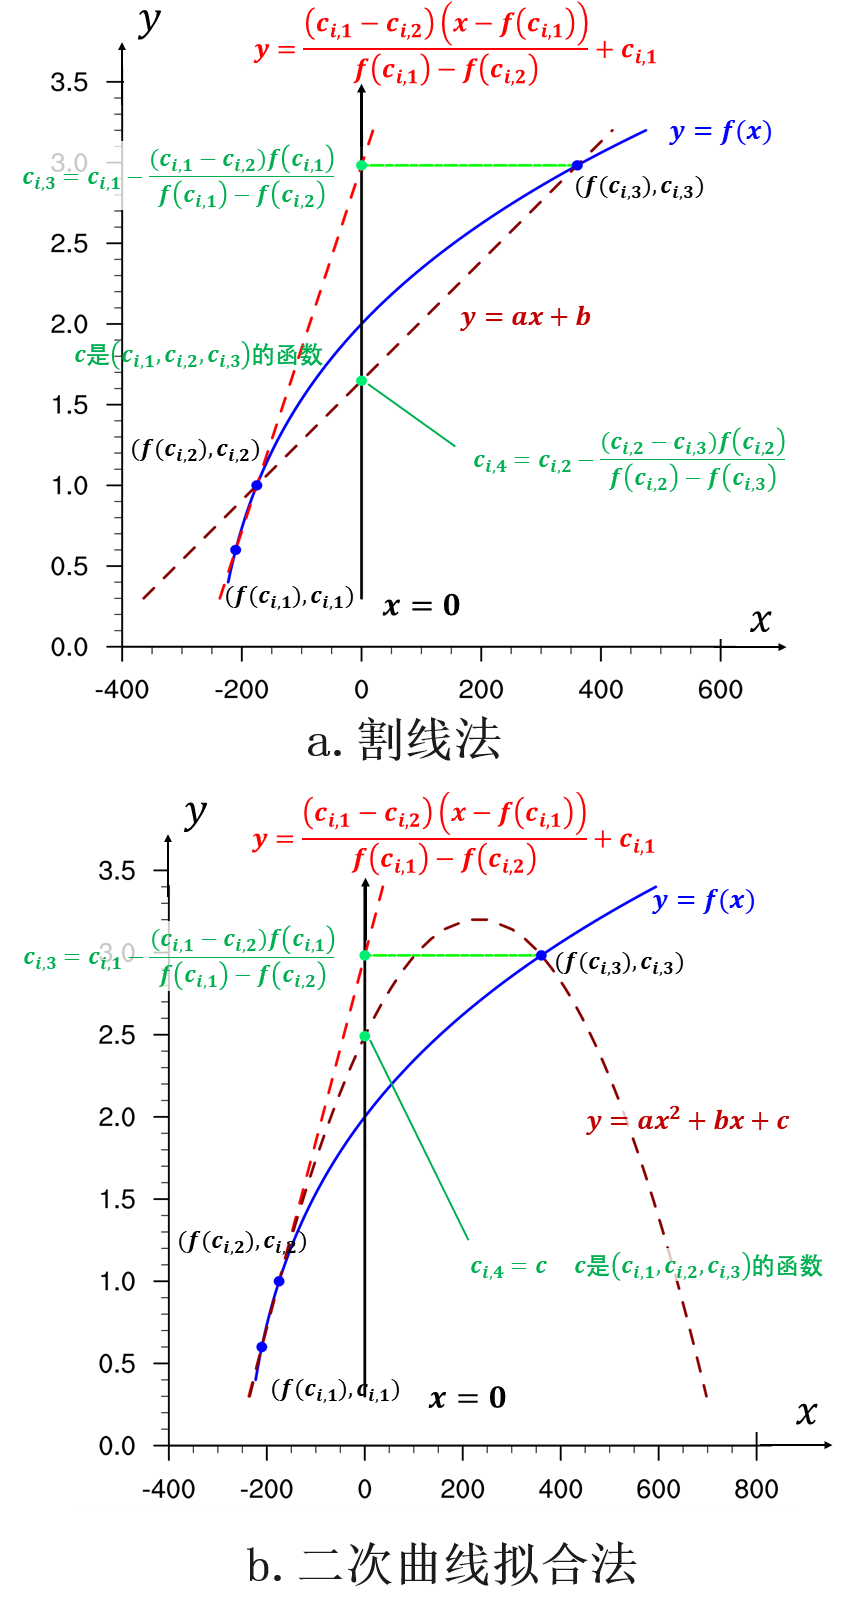
\includegraphics[width=0.56\textwidth]{Figures/气孔导度和光合作用/光合气孔耦合模型数值解法示意图.png}
\caption[光合气孔耦合模型数值解法示意图]{光合气孔耦合模型数值解法示意图,割线法对前两次迭代结果进行线性拟合,拟合结果和$x=0$的交点即为下一轮迭代的胞间$\rm CO_2$浓度的取值,拟合方程$y=ax+b$;二次方程拟合法对前三次迭代结果进行二次曲线拟合,拟合结果和$x=0$的交点即为下一轮迭代的胞间$\rm CO_2$浓度的取值,拟合方程$y=ax^2+bx+c$。

其中割线法的拟合方程系数为:

$\begin{cases}a=\frac{c_{{\mathrm i},n-1}-c_{{\mathrm i},n-2}}{f\left(c_{{\mathrm i},n-1}-c_{{\mathrm i},n-2}\right)}\\b=c_{{\mathrm i},n-2}-a\cdot f\left(c_{{\mathrm i},n-2}\right)\end{cases}$

二次方程拟合法的拟合方程系数为:

$\begin{cases}a=\frac{\left(c_{{\mathrm i},n-2}-c_{{\mathrm i},n-3}\right)-\left[f\left(c_{{\mathrm i},n-2}\right)-f\left(c_{{\mathrm i},n-3}\right)\right]b}{f^2\left(c_{{\mathrm i},n-2}\right)-f^2\left(c_{{\mathrm i},n-3}\right)}\\
b=\frac{\left(c_{{\mathrm i},n-2}-c_{{\mathrm i},n-3}\right)\left[f^2\left(c_{{\mathrm i},n-1}\right)-f^2\left(c_{{\mathrm i},n-2}\right)\right]-\left(c_{{\mathrm i},n-1}-c_{{\mathrm i},n-2}\right)\left[f^2\left(c_{{\mathrm i},n-2}\right)-f^2\left(c_{{\mathrm i},n-3}\right)\right]}{\left[f\left(c_{{\mathrm i},n-2}\right)-f\left(c_{{\mathrm i},n-3}\right)\right]\left[f^2\left(c_{{\mathrm i},n-1}\right)-f^2\left(c_{{\mathrm i},n-2}\right)\right]-\left[f\left(c_{{\mathrm i},n-1}\right)-f\left(c_{{\mathrm i},n-2}\right)\right]\left[f^2\left(c_{{\mathrm i},n-2}\right)-f^2\left(c_{{\mathrm i},n-3}\right)\right]}\\
c=c_{{\mathrm i},n-2}-af^2\left(c_{{\mathrm i},n-2}\right)-bf\left(c_{{\mathrm i},n-2}\right)\end{cases}$}
\label{fig:光合气孔耦合模型数值解法示意图}
\end{figure}
}

对目标函数的零点搜索过程中,我们采用割线法和二次方程拟合法,两种方法相结合的办法(如图~\ref{fig:光合气孔耦合模型数值解法示意图})。在割线法中,$c_{\mathrm{i,sun,se},n}$和$c_{\mathrm{i,sha,se},n}$是第$n$次迭代的胞间$\rm CO_2$浓度,存在与任意两次之前迭代结果(不妨设为第$k$次和第$l$次)的递推关系:
\begin{equation}\label{cisunn}
c_{\mathrm{i,sun,se},n}=c_{\mathrm{i,sun,se},k}-f_{1}\left(c_{\mathrm{i,sun,se},k}\right)\frac{c_{\mathrm{i,sun,se},k}-c_{\mathrm{i,sun,se},l}}{ f_{1}\left(c_{\mathrm{i,sun,se},k}\right)-f_{1}\left(c_{\mathrm{i,sun,se},l}\right)}
\end{equation}
\begin{equation}\label{cishan}
c_{\mathrm{i,sha,se},n}=c_{\mathrm{i,sha,se},k}-f_{2}\left(c_{\mathrm{i,sha,se},k}\right)\frac{c_{\mathrm{i,sha,se},k}-c_{\mathrm{i,sha,se},l}}{ f_{2}\left(c_{\mathrm{i,sha,se},k}\right)-f_{2}\left(c_{\mathrm{i,sha,se},l}\right)}
\end{equation}

在二次方程拟合法中,$c_{\mathrm{i,sun,qd},n}$和$c_{\mathrm{i,sha,qd},n}$是第$n$次迭代的胞间$\rm CO_2$浓度,可由任意三次之前迭代的结果(不妨设为第$k$次,第$l$次和第$m$次)推导而出:
\begin{equation}\label{cisunq}
c_{\mathrm{i,sun,qd},n} =c_{\mathrm{i,sun,qd},l} \\
  -a_{\mathrm{\mathrm{sun}}}\cdot f^2_{1}(c_{\mathrm{i,sun,qd},l}) - b_{\mathrm{\mathrm{sun}}}\cdot f_{1}(c_{\mathrm{i,sun,qd},l})
\end{equation}
\begin{equation}\label{cishaq}
c_{\mathrm{i,sha,qd},n} =c_{\mathrm{i,sha,qd},l} \\
  -a_{\mathrm{\mathrm{sha}}}\cdot f^2_{2}(c_{\mathrm{i,sha,qd},l}) - b_{\mathrm{\mathrm{sha}}}\cdot f_{2}(c_{\mathrm{i,sha,qd},l})
\end{equation}
%
其中$a_{\mathrm{sun}}$,$a_{\mathrm{sha}}$,$b_{\mathrm{sun}}$和$b_{\mathrm{sha}}$分别由前两次和前三次迭代结果递推而得:
\begin{equation}\label{iterbsun}
b_{\mathrm{sun}} = \frac{\Delta c_{\mathrm{i,sun}}\left(k,l\right)\Delta f^2_1\left(l,m\right)-\Delta c_{\mathrm{i,sun}}(l,m) \Delta f^2_1\left(k,l\right)}{\Delta f^2_1\left(l,m\right) \Delta f_1 \left(k,l\right)-\Delta f^2_1\left(k,l\right)\Delta f_1 \left(l,m\right)}
\end{equation}
\begin{equation}\label{iterasun}
a_{\mathrm{sun}} = \frac{\left(c_{\mathrm{i,sun,dq},k}-c_{\mathrm{i,sun,dq},l}\right)-\left[f_1(c_{\mathrm{i,sun,dq},k})-f_1(c_{\mathrm{i,sun,dq},l})\right]\cdot b_{\mathrm{\mathrm{sun}}}}{f^2_1(c_{\mathrm{i,sun,dq},k})-f^2_1(c_{\mathrm{i,sun,dq},l})}
\end{equation}
\begin{equation}\label{iterbsha}
b_{\mathrm{sha}} = \frac{\Delta c_{\mathrm{i,sha}}\left(k,l\right)\Delta f^2_2\left(l,m\right)-\Delta c_{\mathrm{i,sha}}(l,m) \Delta f^2_2\left(k,l\right)}{\Delta f^2_2\left(l,m\right) \Delta f_2 \left(k,l\right)-\Delta f^2_2\left(k,l\right)\Delta f_2 \left(l,m\right)}
\end{equation}
\begin{equation}\label{iterasha}
a_{\mathrm{sha}} = \frac{\left(c_{\mathrm{i,sha,dq},k}-c_{\mathrm{i,sha,dq},l}\right)-\left[f_1(c_{\mathrm{i,sha,dq},k})-f_1(c_{\mathrm{i,sha,dq},l})\right]\cdot b_{\mathrm{\mathrm{sha}}}}{f^2_1(c_{\mathrm{i,sha,dq},k})-f^2_1(c_{\mathrm{i,sha,dq},l})}
\end{equation}
$\Delta$ 用于表示之前第$p$次和第$q$次迭代结果之间的差值:
\begin{equation}
\Delta c_{\mathrm{i,sun}}(p,q)\equiv c_{\mathrm{i,sun,qd},p} - c_{\mathrm{i,sun,qd},q}
\end{equation}
\begin{equation}
\Delta c_{\mathrm{i,sha}}(p,q)\equiv c_{\mathrm{i,sha,qd},p} - c_{\mathrm{i,sha,qd},q}
\end{equation}
\begin{equation}
\Delta f_1 \left(p,q\right)\equiv f_1(c_{\mathrm{i,sun,qd},p})-f_1(c_{\mathrm{i,sun,qd},q})
\end{equation}
\begin{equation}
\Delta f_2 \left(p,q\right)\equiv f_2(c_{\mathrm{i,sha,qd},p})-f_2(c_{\mathrm{i,sha,qd},q})
\end{equation}
\begin{equation}
\Delta f^2_1 \left(p,q\right)\equiv f^2_1(c_{\mathrm{i,sun,qd},p})-f^2_1(c_{\mathrm{i,sun,qd},q})
\end{equation}
\begin{equation}
\Delta f^2_2 \left(p,q\right)\equiv f^2_2(c_{\mathrm{i,sha,qd},p})-f^2_2(c_{\mathrm{i,sha,qd},q})
\end{equation}
另外,$k$,$l$和$m$的选择见数值方案解法流程图 (图~\ref{fig:气孔数值解法流程图})。

对于割线法来说,因为要运用方程~\eqref{cisunn} 和~\eqref{cishan} 对胞间$\rm CO_2$浓度进行猜解,需要至少两次之前迭代的结果。所以,胞间$\rm CO_2$浓度的前两次初始迭代的取值($c_{\mathrm{i,sun,1}}$,$c_{\mathrm{i,sha,1}}$,$c_{\mathrm{i,sun,2}}$和$c_{\mathrm{i,sha,2}}$)需要预先给定;对于二次方程拟合方法来说,因为方程~\eqref{cisunq} 和~\eqref{cishaq} 需要三次之前迭代的结果进行拟合,前三次初始迭代的胞间$\rm CO_2$浓度的取值也需要预先给定。由于两种方法都需要至少两次初始迭代结果,我们令割线法和二次方程拟合法的前两次初始迭代的胞间$\rm CO_2$浓度取值一致。

胞间$\rm CO_2$浓度的第1个初始迭代取值($c_{\mathrm{i,sun,1}}$和$c_{\mathrm{i,sha,1}}$),按C3、C4植物类型区分:
\begin{align}\label{ci_1}
\begin{cases}
c_{\mathrm{i,sun,1}}=c_{\mathrm{i,sha,1}}=\frac{0.25 \cdot o_{\mathrm{i}}} {2600 \cdot 0.57 ^\frac{T_{\mathrm{{leaf }}} -  T_{\mathrm{o p}}}{10}} + 0.5\cdot c_{\mathrm{a}}\cdot\left(1-\frac{1.6}{m}\right) &\rm for\,\, C3\\
c_{\mathrm{i,sun,1}}=c_{\mathrm{i,sha,1}}=0.5\cdot c_{\mathrm{a}}\cdot\left(1-\frac{1.6}{m}\right)   &\rm for\,\, C4
\end{cases}
\end{align}

胞间$\rm CO_2$浓度的第2个初始迭代取值($c_{\mathrm{i,sun,2}}$和$c_{\mathrm{i,sha,2}}$),和C3、C4植物类型和第一次猜解结果$f_{1}\left(c_{\mathrm{i,sun,1}}\right)$,$f_{2}\left(c_{\mathrm{i,sha,1}}\right)$的符号有关,这是为了让目标函数尽量接近0点:

如果$f_{1}\left(c_{\mathrm{i,sun,1}}\right)\geqslant 0$则阳叶胞间$\mathrm {CO_2}$浓度的第二次迭代取值为:
\begin{align}\label{cisun_2_fp}
c_{\mathrm{i,sun,2}}=
\begin{cases}
\frac{0.4 \cdot o_{\mathrm{i}}} {2600 \cdot 0.57 ^\frac{T_{\mathrm{{leaf }}} -  T_{\mathrm{o p}}}{10}} + 0.2\cdot c_{\mathrm{a}}\cdot\left(1-\frac{1.6}{m}\right)  &\rm for\,\, C3\\
0.2\cdot c_{\mathrm{a}}\cdot\left(1-\frac{1.6}{m}\right) &\rm for\,\, C4
\end{cases}
\end{align}

如果$f_{2}\left(c_{\mathrm{i,sha,1}}\right)\geqslant0$,则阴叶胞间$\mathrm {CO_2}$浓度的第二次迭代取值为:
\begin{align}\label{cisha_2_fp}
c_{\mathrm{i,sha,2}}=
\begin{cases}
\frac{0.4 \cdot o_{\mathrm{i}}} {2600 \cdot 0.57 ^\frac{T_{\mathrm{{leaf }}} -  T_{\mathrm{o p}}}{10}} + 0.2\cdot c_{\mathrm{a}}\cdot\left(1-\frac{1.6}{m}\right)  &\rm for\,\, C3\\
0.2\cdot c_{\mathrm{a}}\cdot\left(1-\frac{1.6}{m}\right) &\rm for\,\, C4
\end{cases}
\end{align}

如果$f_{1}\left(c_{\mathrm{i,sun,1}}\right)<0$,则阳叶胞间$\mathrm {CO_2}$浓度的第二次迭代取值为:
\begin{align}\label{cisun_2_fn}
c_{\mathrm{i,sun,2}}=
\begin{cases}
\frac{0.1 \cdot o_{\mathrm{i}}} {2600 \cdot 0.57 ^\frac{T_{\mathrm{{leaf }}} -  T_{\mathrm{o p}}}{10}} + 0.8\cdot c_{\mathrm{a}}\cdot\left(1-\frac{1.6}{m}\right)  &\rm for\,\, C3\\
0.8\cdot c_{\mathrm{a}}\cdot\left(1-\frac{1.6}{m}\right) &\rm for\,\, C4
\end{cases}
\end{align}

如果$f_{2}\left(c_{\mathrm{i,sha,1}}\right)<0$,则阴叶胞间$\mathrm {CO_2}$浓度的第二次迭代取值为:
\begin{align}\label{cisha_2_fn}
c_{\mathrm{i,sha,2}}=
\begin{cases}
\frac{0.1 \cdot o_{\mathrm{i}}} {2600. \cdot 0.57 ^\frac{T_{\mathrm{{leaf }}} -  T_{\mathrm{o p}}}{10}} + 0.8\cdot c_{\mathrm{a}}\cdot\left(1-\frac{1.6}{m}\right)  &\rm for\,\, C3\\
0.8\cdot c_{\mathrm{a}}\cdot\left(1-\frac{1.6}{m}\right) &\rm for\,\, C4
\end{cases}
\end{align}

二次方程拟合法的第三次迭代胞间$\mathrm {CO_2}$浓度取值由割线法,按方程~\eqref{cisunn} 和~\eqref{cishan}计算得到:
%
\begin{equation}\label{cisun3}
c_{\mathrm{i,sun,qd,3}}=c_{\mathrm{i,sun,1}}-f_{1}\left(c_{\mathrm{i,sun,1}}\right)\frac{c_{\mathrm{i,sun,1}}-c_{\mathrm{i,sun,2}}}{ f_{1}\left(c_{\mathrm{i,sun,1}}\right)-f_{1}\left(c_{\mathrm{i,sun,2}}\right)}
\end{equation}
\begin{equation}\label{cisha3}
c_{\mathrm{i,sha,qd,3}}=c_{\mathrm{i,sha,1}}-f_{2}\left(c_{\mathrm{i,sha,1}}\right)\frac{c_{\mathrm{i,sha,1}}-c_{\mathrm{i,sha,2}}}{ f_{2}\left(c_{\mathrm{i,sha,1}}\right)-f_{2}\left(c_{\mathrm{i,sha,2}}\right)}
\end{equation}

三次初始迭代以后,迭代所估计的每一步胞间$\rm CO_2$浓度$\left(c_{\mathrm{i,sun},k}和c_{\mathrm{i,sha},k}\right)$由割线法和二次方程拟合法的平均值共同确定:
\begin{equation}
c_{\mathrm{i,sun},k}=\frac{c_{\mathrm{i,sun,se},k}+c_{\mathrm{i,sun,qd},k}}{2}
\end{equation}
\begin{equation}
c_{\mathrm{i,sha},k}=\frac{c_{\mathrm{i,sha,se},k}+c_{\mathrm{i,sha,qd},k}}{2}
\end{equation}

光合气孔耦合模型求解迭代算法的总体流程如流程图\ref{fig:气孔数值解法流程图}所示,包含一下几个步骤和规则:
\begin{enumerate}
\item
根据方程~\eqref{ci_1}--\eqref{cisha3},分别计算最初三次迭代的胞间$\rm CO_2$浓度;
\item
根据方程~\eqref{f1_cisun} 和~\eqref{f1_cisha} 和胞间$\rm CO_2$浓度初始值,计算前三次初始迭代的目标函数$f_1\left(c_{\mathrm{i,sun},k}\right)$,$f_2\left(c_{\mathrm{i,sha},k}\right)$ $\left(k=1,2,3\right)$;
\item
记录已有迭代结果按目标函数值进行排序,并找到最接近零点的两次(割线法)或三次迭代结果(二次方程拟合法),计算下一迭代的胞间$\rm CO_2$浓度;
\item
根据胞间$\rm CO_2$浓度猜解,计算一迭代的目标函数。
\item
判断目标函数是否满足退出条件,如果目标函数的绝对值小于阈值0.1,则停止迭代,否则,重复步骤3--5。最终结果将保存最后一次迭代的各个状态。
\end{enumerate}
此外,步骤5的迭代退出判断不仅在步骤4之后进行,在初始迭代的目标函数计算之后同样需要判断退出条件。

{
\begin{figure}[htbp]
\centering
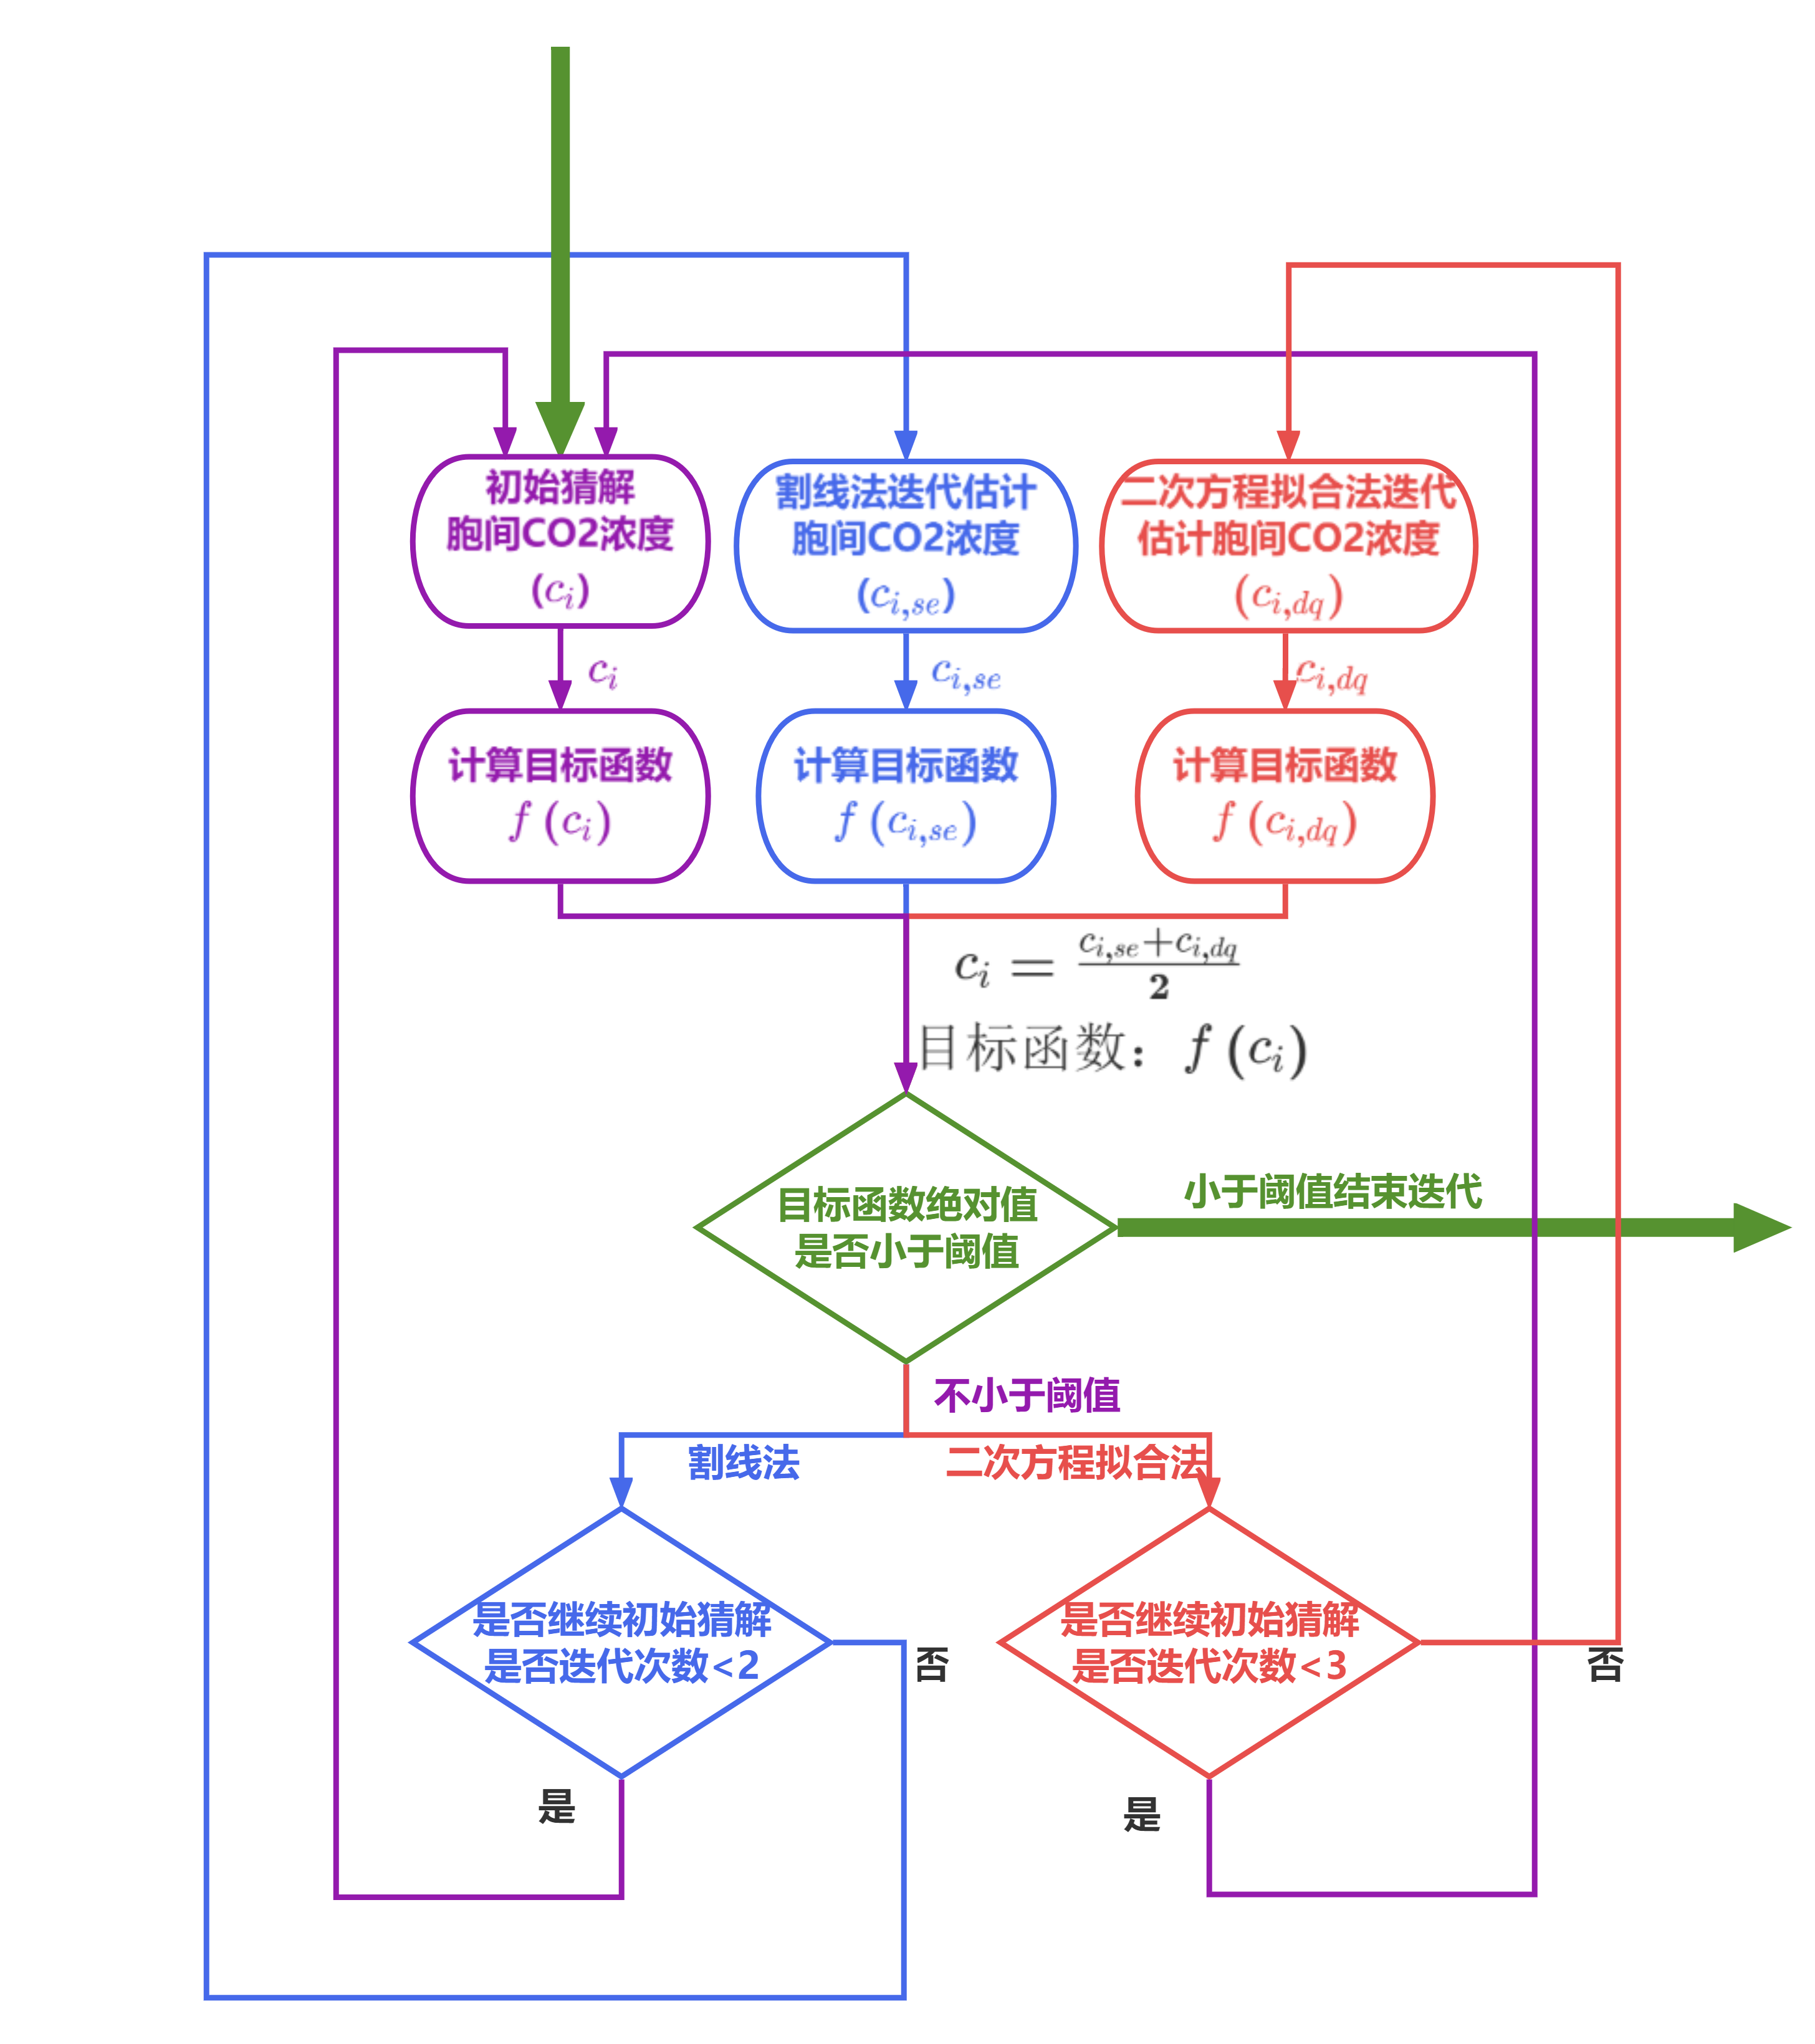
\includegraphics[width=0.9\textwidth]{Figures/气孔导度和光合作用/气孔数值解法流程图.png}
\caption{气孔数值解法流程图}
\label{fig:气孔数值解法流程图}
\end{figure}
}

\chapter{植被水力模式}
%\addcontentsline{toc}{chapter}{植被水力模式}

%\begin{植被水力模式}
CoLM植物水力模式根据土壤-植物-大气连通体的概念计算陆气水分交换的蒸腾分量。
CoLM植物水力模式中的植物水分传输得益于土壤、根、茎和叶之间形成的水势梯度。植物各部位的水势也密切影响着各植物水力过程。
首先,根、茎、叶的水势通过植物栓塞过程影响着植物水分传输能力 (详见章节 \ref{植物水力导度的衰减})。
其次,植物根与每层土壤的水势梯度将影响根的水力重分配过程 (详见章节 \ref{地下植物水力过程})。最后,叶片的水势降低将影响叶片气孔导度,
同时影响植物水分传输和光合作用 (详见章节 \ref{气孔导度的水分胁迫})。


\section{植物水势动态}\label{植物水势动态}
植物水势的动态模拟是CoLM植物水力模式的关键。CoLM植物水力模式的水势模拟包括地上和地下植物水力过程两部分
。地上部分包括在阳叶、阴叶、茎和地表根四个节点的水势 ($\Psi_{sunleaf}$,$\Psi_{shaleaf}$,$\Psi_{stem}$,$\Psi_{root,0}$)

 模拟;地下部分包括地表根以及$n$层地下根 $n+1$个节点的水势 ($\Psi_{root,i}$,$i=0,1,2,\ldots,n$) 模拟。地上、地下两部分通过地表根水势
 ($\Psi_{root,0}$)的模拟被密切的耦合(如图~\ref{fig:CoLM植物水力模型示意图})。

 {
\begin{figure}[htbp]
\centering
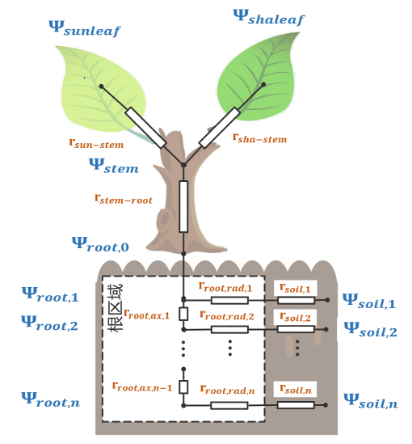
\includegraphics{Figures/植被水力模式/CoLM植物水力模型示意图.png}
\caption{CoLM植物水力模型示意图。}
\label{fig:CoLM植物水力模型示意图}
\end{figure}
}


CoLM植物水势的动态模拟假设植物水分传输为稳恒流,并将其类比为电路问题~
\citep{van1948water},即水分传输速率正比于水势差和水力导度。
地上部分四个节点的水势由Darcy定律表达,满足以下方程:
\begin{equation}\label{q_sunstem}
q_{ {sun \leftarrow stem }}=k_{{sun} \leftarrow  {stem}}\left(\Psi_{sunleaf}-\Psi_{stem}\right)
\end{equation}
\begin{equation}
q_{ {sha \leftarrow stem }}=k_{ {sha} \leftarrow {stem}}\left(\Psi_{shaleaf}-\Psi_{ {stem }}\right)
\end{equation}
\begin{equation}
q_{ {stem \leftarrow root }}=k_{ {stem } \leftarrow  { root }}\left(\Psi_{ {stem }}-\Psi_{ {root }, 0}\right)
\end{equation}
$k_{sun \leftarrow stem}$,$k_{sha \leftarrow stem }$,$k_{stem \leftarrow root }$ 分别代表茎到阳叶的水力导度、茎到阴叶的水力导度和根到茎的水力导度。
水力导度随水势降低而降低,是关于茎和根水势的函数 (详见章节~\ref{植物水力导度的衰减}) 。地表根水势$\Psi_{root,0}$是关于每层土壤水势 ($\Psi_{soil,i}$) 
及根总吸水速率 ($q_{root,0}$) 的函数,由地下植物水力过程所计算 (详见章节~\ref{地下植物水力过程}):
\begin{equation}\label{Psi_root_0}
\Psi_{root, 0}=R\left(\Psi_{ {soil }, i}, q_{root, 0}\right)
\end{equation}
$q_{sun \leftarrow stem}$,$q_{sha \leftarrow stem }$,$q_{stem \leftarrow root }$分别代表茎到阳叶的水流速、茎到阴叶的水流速和根到茎的水流速。
水流速在各节点由于稳恒流假设,满足水分守恒方程:
\begin{equation}
E_{sun}=q_{sun \leftarrow  stem}
\end{equation}
\begin{equation}
E_{ {sha }}=q_{ sha \leftarrow stem}
\end{equation}
\begin{equation}
q_{ {sun \leftarrow stem }}+q_{ {sha \leftarrow stem }}=q_{ {stem \leftarrow root }}
\end{equation}
\begin{equation}\label{q_stemroot}
q_{stem \leftarrow root}=q_{root, 0}
\end{equation}
$E_{sun}$代表阳叶蒸腾速率,$E_{sha}$代表阴叶蒸腾速率。它们是由无水分胁迫情况下的叶片蒸腾 ($E_{sun,max}$, $E_{sha,max}$) 
和受叶片水势 ($\Psi_{sunleaf}$,$\Psi_{shaleaf}$) 控制的蒸腾衰减函数所组成(详见章节~\ref{植物水力导度的衰减})。
同时,无水分胁迫的叶片蒸腾是在最大气孔导度 ($g_{s,sun,max}$, $g_{s,sha,max}$) 的条件下,
运用章节~\ref{一维植被湍流交换模型} 植被覆盖地表湍流通量的计算方案所推导得出。最大气孔导度的计算则需要植物水力模式、光合作用模式、气孔导度模式耦合解出 (详见章节~\ref{气体扩散方程和气孔导度模型})。


\section{植物水力导度的衰减}\label{植物水力导度的衰减}
植物水势下降导致的空穴现象会严重降低水分在植物内部的传导能力。我们将实验上观测到水力导度随水势变化的S型脆弱性曲线 
\citep{sperry1988method,gentine2016allometry,neufeld1992genotypic,pammenter1998mathematical,plaut2012hydraulic}
 引入到模型,对植物水力栓塞进行参数化,得到节点间的水力导度$k_{i\gets j}$ (从节点$j$到$i$的传输):
\begin{equation}
k_{i \leftarrow j}=k_{\max } \cdot 2^{-\left(\frac{\Psi_{\mathbf{j}}}{p 50}\right)^{c_{k}}}
\end{equation}
其中$k_{max}$表示最大水力导度 (\unit{s^{-1}})。$\Psi_j$代表节点$j$的水势 (\unit{mm.H_2O}),$p50$代表水力导度降低 50\% 时的水势 (\unit{mm.H_2O}),$c_k$代表脆弱性曲线的形状参数。


实验数据发现气孔导度和叶片水势同样存在S型曲线关系 \citep{klein2014variability},
CoLM植物水力模式引入蒸腾速率随叶片水势 ($\Psi_{sunleaf}$,$\Psi_{shaleaf}$)的衰减函数 \citep{kennedy2019implementing}:
\begin{equation}\label{e_sun_a}
E_{ {sun }}=E_{ {sun,max }} \cdot 2^{-\left(\frac{\Psi_{ {sunleaf }}}{p 50}\right)^{c_{k}}}
\end{equation}
\begin{equation}\label{e_sha_a}
E_{ {sha }}=E_{ {sha,max }} \cdot 2^{-\left(\frac{\Psi_{ {shaleaf }}}{p 50}\right)^{c_{k}}}
\end{equation}
$E_{sun,max} $和$E_{sha,max}$分别表示无水分胁迫情况下的阳叶、阴叶的最大蒸腾速率。


\section{地下植物水力过程}\label{地下植物水力过程}
水力重分配是重要的植物地下水力过程,它描述了水分通过地下根系从湿润土壤层向干燥土壤层的传输。
它被认为是一个被动的受水势梯度所驱动的水分传输过程。基于该物理原理,Amenu水力重分配模型 \citep{amenu2008}被CoLM采用 \citep{zhu2017incorporating},
并与土壤水文过程和植被地上水力过程相耦合 \citep{li2021new},考虑包括在根、茎和叶等地上节点外的, 
$n$个代表不同土壤深度的根系水力节点和$n$个土壤水力节点 (如图~\ref{fig:CoLM植物水力模型示意图})。模式中的水力传导包括轴向水力传导和径向水力传导。
轴向水力传导由Darcy定律所表示:
\begin{equation}\label{k_axi}
k_{ax,i}\left(\Psi_{r,i}-\Psi_{r,i+1}\right)=q_{ax,i}
\end{equation}
其中$k_{ax,i}$代表第$i+1$层到第i层根节点间的轴向水力导度,$q_{ax,i}$代表相应的轴向水分传输速率,
$\Psi_{r,i}$代表第$i$层根节点的水势。$i$取值1到$n-1$,$n$代表土壤总层数。\\
径向水力传导方程:
\begin{equation}\label{k_radi}
k_{rad,i}\left(\Psi_{soil,i}-\Psi_{r,i}\right)=q_{rad,i}
\end{equation}
其中$k_{rad,i}$代表第$i$层土壤节点到根节点间的径向水力导度,
$q_{rad,i}$代表相应的径向水分传输速率,$\Psi_{soil,i}$代表第$i$层土壤节点的水势,$i$取值1到$n$。



对于第2到$n$层的土壤根节点存在水分平衡方程:
\begin{equation}\label{q_axi}
q_{a x, i}+q_{r a d, i}=q_{a x, i-1}
\end{equation}
其中$i=2, \ldots, n$,方程~\eqref{q_axi} 实际上是$n-1$个方程组。


另外,由表层根节点的水分平衡方程可得:
\begin{equation}\label{q_ax1}
q_{ax,1}+q_{rad, 1}=q_{root,0}
\end{equation}
将方程(\ref{k_axi})和(\ref{k_radi})代入(\ref{q_axi})和(\ref{q_ax1}),则得到关于$ \Psi_{r,i}$的$n$个线性方程组。
这$n$个线性方程组描述了在植物地下水力过程作用下,根水势垂直分布。其输入包括土壤水势垂直分布 ($\Psi_{soil,i}$) 和根总吸水速率 ($q_{root,0}$)。
其输出包括根水势垂直分布 ($\Psi_{r,i}$) 和根吸水速率垂直分布 ($q_{rad,i}$)。因此,地下植物水力过程可以被简化地表示为公式(\ref{Psi_root_0})。


\section{气孔导度的水分胁迫}\label{气孔导度的水分胁迫}
土壤水分亏缺对植物生理的影响被表现在水分胁迫因子上,水分胁迫因子作为取值 $0\sim 1$ 的无量纲变量,作用在光合作用各限制因子上,见公式(\ref{V_cmax_a})--(\ref{R_d1})。

植物水力模式未开启时,水分胁迫因子 ($\beta$) 决定于根的垂直分布比例和土壤水势,其计算不区分阴叶和阳叶:
\begin{equation}\label{beta_0}
\beta=\sum_{i=1}^{n} froot_i \beta_{i}
\end{equation}

\begin{equation}\label{beta_i}
\beta_{i}=\frac{\Psi_{\max }-\Psi i}{\Psi_{\max }-\Psi_{s a t}}
\end{equation}
$froot_i$是第i层的根含量,$\beta_i$是第$i$层的水分胁迫因子;它根据每层土壤的实际水势 (${\Psi}_i$),最大水势 (${\Psi}_{max}$)和饱和水势 (${\Psi}_{sat}$)计算得出。

当植物水力模式开启时,水分胁迫对植被的直接影响是植物水势的降低,气孔通过关闭以尽量保持植物的导水能力,但同时也导致叶片光合速率降低。
植物水力模式符合植物生理学理论和物理规律,水分胁迫因子 ($\beta_{sun}$,$\beta_{sha}$) 决定于气孔导度的衰减比例,其计算区分阳叶和阴叶:
\begin{equation}\label{beta_sun}
\beta_{sun}=g_{s,sun} / g_{s,sun,max }
\end{equation}
\begin{equation}\label{beta_sha}
\beta_{sha}=g_{s,sha} / g_{s,sha, \max }
\end{equation}
$g_{s,sun}$和$g_{s,sun}$分别代表阳叶和阴叶的实际气孔导度,
$g_{s,sun,max}$和$g_{s,sun,max}$分别代表阳叶和阴叶在无水分胁迫条件下的最大气孔导度。
水分胁迫的求解需要耦合地表冠层湍流参数化方案和光合气孔模式。


最大气孔导度 ($g_{s,sun,max}$和$g_{s,sun,max}$) 的计算依赖于光合气孔模式。
光合气孔模式中,气孔导度为方程(\ref{ei_cs})的正根,(\ref{ei_cs})和(\ref{ci_1})联立可表示为实际气孔导度关于净光合作用速率的隐式方程:
\begin{equation}\label{gs_0}
g_{s}=g\left(A_{n}\right)
\end{equation}
由于水分胁迫是光合作用中的相关参数,公式(\ref{gs_0})可以写成:
\begin{equation}\label{gs_1}
g_{s}=g\left(f_{photo}(\beta)\right)
\end{equation}
最大气孔导度可表述为:
\begin{equation}\label{gs_sunmax}
g_{s,  { sun,max }}=\frac{g\left(f_{ {photo }}\left(\beta_{ {sun }}\right)\right)}{\beta_{ {sun }}}
\end{equation}
\begin{equation}\label{gs_shamax}
g_{s, sha, \max }=\frac{g\left(f_{photo}\left(\beta_{s h a}\right)\right)}{\beta_{s h a}}
\end{equation}
$f_{photo}$代表公式(\ref{An1})的光合作用模型。


最大气孔导度一方面是植物水力模式水分胁迫计算的必要变量(公式(\ref{beta_sun})和(\ref{beta_sun})),
另一方面,为地表冠层湍流参数化方案中叶片最大蒸腾速率计算提供重要输入 (如图~\ref{fig:光合气孔模式和植物水力模式的耦合示意图})。
地表冠层湍流参数化方案中的叶片最大蒸腾速率$(E_{sun,max}$和$E_{sha,max}$) 可简化地表示为:
\begin{equation}\label{E_sunmax}
E_{sun, \max }=E\left(g_{s, sun, \max }\right)
\end{equation}
\begin{equation}\label{E_shamax}
E_{sha, \max }=E\left(g_{s, sha, \max }\right)
\end{equation}
其中,与植物水力模式无关的参数、变量在此省略,完整表述见植被覆盖地表湍流通量的计算方案 (见章节 \ref{一维植被湍流交换模型})。


实际气孔导度 ($g_{s,sun}$和$g_{s,sun}$) 的计算同样依赖于地表冠层湍流参数化方案。由于植物水力模式可以求解植物叶片实际蒸腾 ($E_{sun}$和$E_{sha}$),
可以利用公式(\ref{E_sunmax})和(\ref{E_shamax})的逆函数求解气孔导度:
\begin{equation}\label{g_ssun}
g_{s, s u n}=E^{-1}\left(E_{s u n}\right)
\end{equation}
\begin{equation}\label{g_ssha}
g_{s, sha}=E^{-1}\left(E_{s h a}\right)
\end{equation}
耦合植物水力模式、光合气孔模式和地表冠层湍流参数化方案,再利用公式(\ref{beta_sun})和(\ref{beta_sha})可以完整地求解植物水力模式下的植物水分胁迫 (如图 \ref{fig:光合气孔模式和植物水力模式的耦合示意图})。
{
    \begin{figure}[htbp]
    \centering
    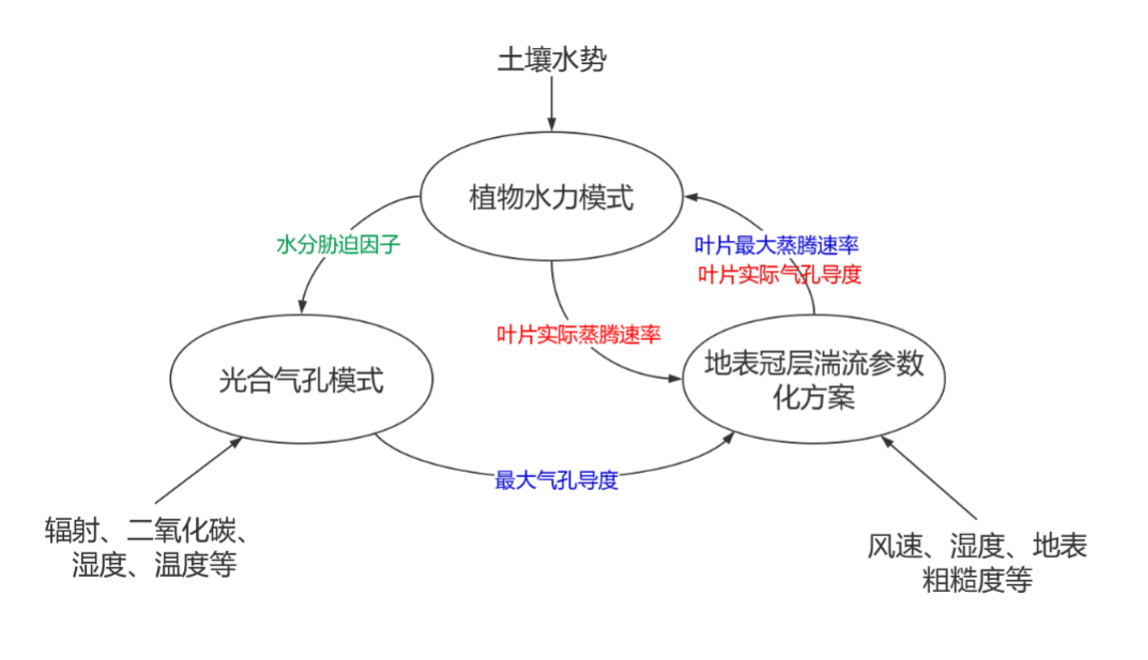
\includegraphics{Figures/植被水力模式/光合气孔模式和植物水力模式的耦合示意图.png}
    \caption{光合气孔模式和植物水力模式的耦合示意图。}
    \label{fig:光合气孔模式和植物水力模式的耦合示意图}
    \end{figure}
}


\section{数值计算方案}\label{数值计算方案}
求解植物水势、水分胁迫、气孔导度和叶片蒸腾速率,需要耦合植物水力模式、光合气孔模式和地表冠层参数化方案。
耦合描述植物水势变化的动力方程组(公式(\ref{q_sunstem})--(\ref{q_stemroot}), (\ref{e_sun_a}) 和(\ref{e_sha_a})),
地表冠层参数化方案 (公式(\ref{E_sunmax})--(\ref{g_ssha})),
光合气孔模式的最大气孔导度计算 (公式(\ref{gs_sunmax})和(\ref{gs_shamax})), 植物水分胁迫计算(公式(\ref{beta_sun})和(\ref{beta_sha})),共18个方程,
求解包括4个植物地上水势节点 ($\Psi_{sunleaf}$, $\Psi_{shaleaf}$, $\Psi_{stem}$和$\Psi_{root,0}$),8个水分传输速率 
($q_{sun-stem}$,$q_{sha-stem}$,$q_{stem-root}$,$q_{root,0}$,$E_{sun}$,$E_{sun,max}$和$E_{sun,max}$) ,4个气孔导度变量
 ($g_{s,sun}$,$g_{s,sun}$,$g_{s,sun,max}$,$g_{s,sun,max}$),2个水分胁迫变量 ($\beta_{sun}$,$\beta_{sha}$) 在内的共18个未知量。

然而,由于以上18个方程中存在隐形方程,我们求解该问题时,引入三重嵌套数值求解办法。其主要步骤如下(图 \ref{fig:植物水力模式的数值模拟流程图}):
\begin{enumerate}
    \item 利用冠层模型,计算叶片温度 ($T_{l,sun}$,$T_{l,sha}$);
    \item 利用光合气孔模式,计算最大气孔导度 ($g_{s,sun,max}$和$g_{s,sun,max}$);
    \item 根据最大气孔导度,计算叶片最大蒸腾速率 ($E_{sun,max}$和$E_{sun,max}$);
    \item 将叶片最大蒸腾速率输入植物水力模式,计算水分胁迫 ($\beta_{sun}$,$\beta_{sha}$);
    \item 更新光合气孔模式的水分胁迫,迭代计算,判断胞间二氧化碳浓度是否收敛,若收敛,进入第 (6) 步;若不收敛,重复此步骤;
    \item 更新气孔导度,判断阴叶、阳叶水分胁迫是否收敛,若收敛,进入第 (7) 步,若不收敛,回到第 (2) 步;
    \item 更新植物水势和叶片蒸腾,判断叶片温度是否收敛,若收敛,植物水力模式求解完成,若不收敛,回到第 (1) 步。
\end{enumerate}

气孔导度详细迭代

{
    \begin{figure}[htbp]
    \centering
    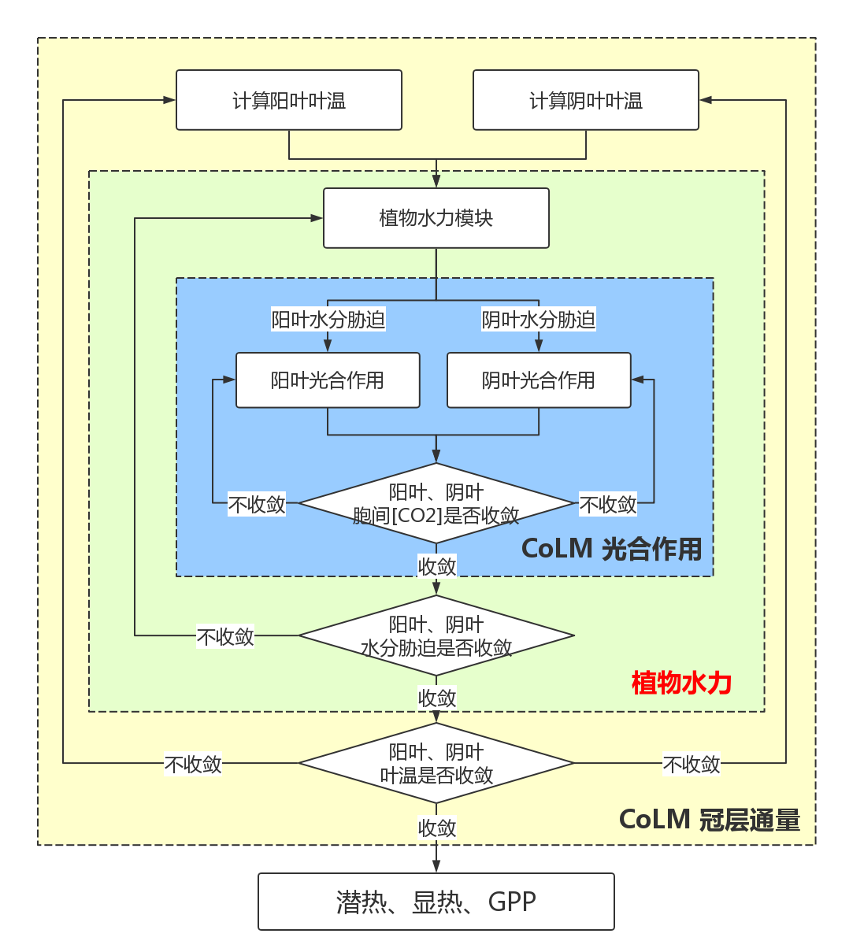
\includegraphics{Figures/植被水力模式/植物水力模式的数值模拟流程图.png}
    \caption{植物水力模式的数值模拟流程图。}
    \label{fig:植物水力模式的数值模拟流程图}
    \end{figure}
}


\chapter{碳氮库结构}\label{碳氮库结构}
%\addcontentsline{toc}{chapter}{碳氮库结构}
\begin{mymdframed}{代码}
本章对应代码源文件位于\texttt{main/BGC/}目录下。
\end{mymdframed}

%\begin{碳氮库结构}
CoLM生物地球化学循环模块模拟陆地生态系统碳氮元素储量的动态变化,随着大气$\rm CO_2$浓度升高,
陆地生态系统碳储量的动态模拟反映出陆地生态系统的累积固碳状况。
由于植被和土壤均具有较为稳定的碳氮比属性,氮元素储量的动态模拟,量化了生态系统固碳的氮限制。
碳氮储量在模型中被分为了21个植被碳库、22个植被氮库、7个土壤凋落物碳库和8个土壤凋落物氮库。
运用箱式模型和碳氮平衡方程,碳氮元素在生态系统的传输网络得以刻画,每个碳氮库的动态变化得以模拟。


根据植被次网格结构,植被碳氮库对土壤碳氮库的共享形式存在差异。
LCT次网格结构中,不存在植物类型间土壤无机氮的竞争,
单个植被类型的一套植被碳氮库(21个植被碳库+ 22个植被氮库)对应一套土壤凋落物碳氮库(7个土壤凋落物碳库+ 8个土壤凋落物氮库)。
PFT次网格结构中,存在植被类型间的土壤无机氮竞争,多个植被功能型的多套植被氮碳库(n个植被功能型×(21个植被碳库+ 22个植被氮库))
共享一套土壤凋落物碳氮库(7个土壤凋落物碳库+ 8个土壤凋落物氮库)。


\section{植被碳氮库结构}\label{植被碳氮库结构}
植被碳库包括叶、细根、活茎、死茎、活粗根和死粗根6个植被营养器官,在接下来章节的公式中,我们用$leaf$, $foot$, $livestem$, $deadstem$, $livecroot$和$deadcroot$代表这6个营养器官。每个植被营养器官包含组织结构库、存储库和传输库3个子库,公式中我们用$disp$, $stor$和$xfer$表示。
因此,每套植被类型有总共18个植被碳库。其中,组织库代表植被营养器官的主要结构组织部分的碳储量,
是植被碳库的主要组成部分;存储碳库和传输碳库分别是长期和短期的非结构碳库,为落叶植被萌发初期提供初始碳,
初始碳供用可以保证植被生长出足够的叶,维持生长季的光合作用。植被氮库除了包含与碳库相对应的18个营养器官氮库之外,
还包含1个再利用氮库,公式中我们用$retran$代表。以刻画植被机体在凋落前回收利用氮的生理机能,因此每套植被类型有总共19个植被氮库。
当作物模式打开时,额外增加谷粒器官的组织库、存储库和传输库。因此,总共21个植被碳库和22个植被氮库。
通过对光合作用碳输入的限制,每个植被的碳库和氮库之间具有相对稳定的碳氮比,详见章节~\ref{植被土壤的氮竞争} 植被土壤的氮竞争。

植被碳库之间或植被氮库之间存在复杂的元素循环网络,见图 \ref{fig:CoLM植被碳氮循环网络示意图}。
植被从光合作用中得到碳,并分配到不同器官。存储库、传输库和组织库的元素循环、
叶和活根的胁迫凋落和季节凋落将在章节 \ref{植被物候过程的耦合预报方案} 植被的物候过程中介绍。
活茎和活粗根每年将有固定比例的碳分别转至死茎和死粗根的碳库中。
死茎和死粗根的周转仅存在于植被的自然死亡或火灾中。
{
\begin{figure}[htbp]
\centering
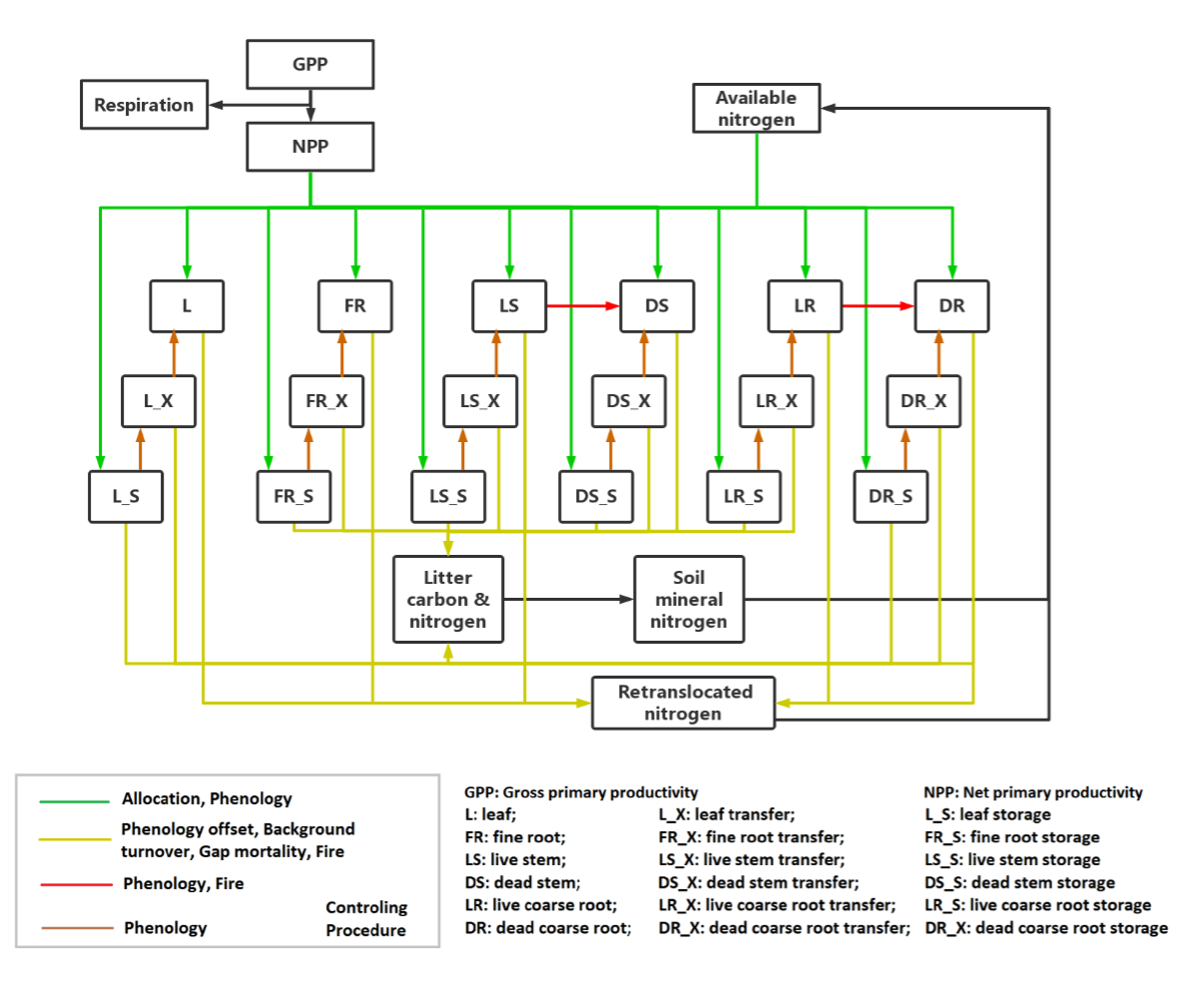
\includegraphics{Figures/碳氮库结构/CoLM植被碳氮循环网络示意图.png}
\caption{CoLM植被碳氮循环网络示意图 \citep{lu2020full}}
\label{fig:CoLM植被碳氮循环网络示意图}
\end{figure}
}

\section{土壤凋落物碳氮库结构}\label{土壤凋落物碳氮库结构}
土壤凋落物的碳储存同样动态模拟,被按照成分和周转时间的长短进行分类,土壤凋落物碳氮库均具有垂直分层结构的刻画。
\subsection{碳氮库分类}\label{碳氮库分类}
土壤凋落物的碳储分为7个有机碳库:代谢凋落物、纤维素凋落物、木质素凋落物、粗木质残体、快速土壤周转库、
慢速土壤周转库和惰性土壤周转库,在公式中我们分别用$met$, $cel$, $lig$, $cwd$, $fast$, $slow$, $pass$来代表。凋落物和快速土壤周转库的周转时间都在几个月到几年之间,粗木质残体、
慢速土壤周转库和惰性土壤周转库的周转时间范围分布可以从几年到上千年,表现出极大的土壤异质性。
氮存储除了以上7个有机库外,还包括1个无机氮库,在公式中用$nmin$表示。由于植被根系吸收只能利用无机氮,无机氮库是连接土壤和植被的枢纽,
土壤和植被对无机氮的竞争将在章节 \ref{植被土壤的氮竞争} 中介绍。


通过从植被库中获取凋落物,地下元素循环从凋落物到土壤存在较为复杂的元素循环网络,
见图 \ref{fig:CoLM土壤凋落物碳氮循环网络示意图}。土壤碳库和土壤氮库之间在循环过程中保持相对稳定的碳氮比,凋落物的碳氮比大于土壤库的碳氮比,
因此缺氮会造成凋落物的分解速率下降,详见章节 \ref{土壤分解的氮限制} 氮限制因子。
{
\begin{figure}[htbp]
\centering
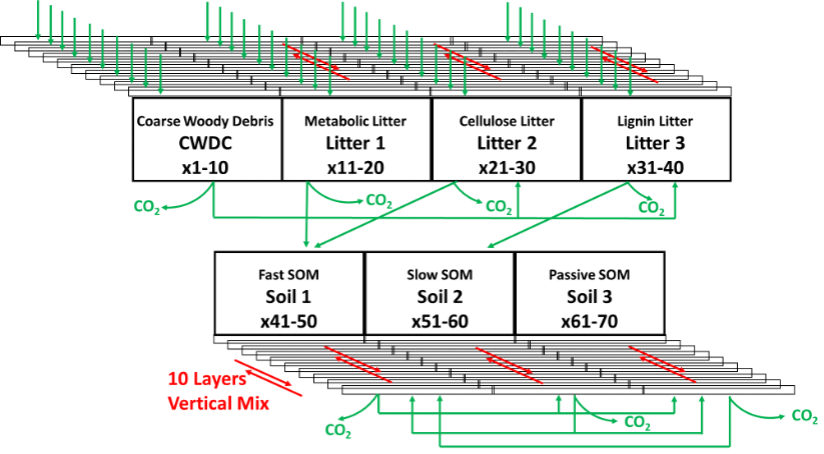
\includegraphics{Figures/碳氮库结构/CoLM土壤凋落物碳氮循环网络示意图.png}
\caption{CoLM土壤凋落物碳氮循环网络示意图 \citep{huang2018matrix}  }
\label{fig:CoLM土壤凋落物碳氮循环网络示意图}
\end{figure}
}
\subsection{垂直分层结构}\label{垂直分层结构}
由于土壤水热条件的垂直差异,土壤碳氮存储垂直分布模拟也极其重要,且与土壤水热条件的垂直分布特点联系紧密。
CoLM模拟土壤和凋落物的碳氮库垂直结构,与土壤水热模拟保持一致,土壤和凋落物的碳氮库垂直方向上也分为10层。
每层土壤和凋落物分别具有不同的输入(叶片和根系的凋落输入)和输出(分解呼吸)。
同时,除了粗木质残体以外的6个有机库均存在碳氮有机物的垂直扩散混合过程,体现了微生物的作用,详见章节 \ref{土壤凋落物的垂直传输} 土壤凋落物的垂直传输过程。

\chapter{植被生物地球化学循环过程}\label{植被生物地球化学循环过程}
%\addcontentsline{toc}{chapter}{植被生物地球化学循环过程}
\begin{mymdframed}{代码}
  本章对应代码源文件位于\texttt{main/BGC/}目录下。
\end{mymdframed}

%\begin{植被生物地球化学循环过程}
CoLM植被生物地球化学循环模块存在复杂的碳氮循环网络,植物生理和物候等过程是量化不同碳氮库相互转换和传输的关键。
光合作用是植被生物地球化学循环的初始输入。光合作用的碳输入扣除植被的自养呼吸得到净初级生产力将被分配到植被不同营养器官中,
植被的自养呼吸和碳氮分配是其中的关键过程。同时,植被生长存在季节变化特征,特别是落叶植被功能型,
物候过程影响植被生物地球化学循环的季节性模拟。物候过程同样模拟叶和细根的凋落过程,
植被碳氮库的周转由物候过程和植被自然死亡过程共同控制。
经过物候过程和植被自然死亡过程,植被凋落物进入土壤进一步进行地下生物地球化学循环。
\section{植被自养呼吸}\label{植被自养呼吸}

CoLM的自养呼吸$CF_{\mathrm{ar,total}}$计算包括维持呼吸$CF_{\mathrm{mr,total}}$和生长呼吸$CF_{\mathrm{gr,total}}$,
模型对他们分别进行模拟 \citep{lavigne1997growth,sprugel1995respiration}。
维持呼吸指植被活体组织维持正常的代谢活动所消耗的碳,生长呼吸指植被生长所消耗的碳。
\begin{equation}
  CF_{\mathrm{ar,total}}=CF_{\mathrm{mr, total}}+CF_{\mathrm{gr,total}}
\end{equation}
\subsection{维持呼吸}
\begin{mymdframed}{代码}
  本节对应的代码文件为\texttt{MOD\_BGC\_Veg\_CNMResp.F90}。
\end{mymdframed}
叶片的维持呼吸($R_{\mathrm {d}} $)由光合作用模块中公式\eqref{R_d1_sun}和\eqref{R_d1_sha}计算。
除此之外,活茎、活粗根和细根同样存在维持呼吸。
维持呼吸和植被器官单位面积的氮含量成正比,同时受到温度的调控:
\begin{equation}
  CF_{\mathrm{{ls}}}=N_{\mathrm{{ls }}} \cdot R_{\mathrm{{b }}} \cdot R_{\mathrm{q10}}^{\left(T_{\mathrm {2m}}-20\right) / 10}
\end{equation}
\begin{equation}
  CF_{\mathrm{ {lr }}}=N_{\mathrm{ {lr }}} \cdot R_{\mathrm{ {b }}} \cdot R_{\mathrm{q10}}^{\left(T_{\mathrm {2m}}-20\right) / 10}
\end{equation}
\begin{equation}
  CF_{\mathrm{ {fr }}}=N_{\mathrm{{fr}}} \cdot R_{\mathrm{{b}}} \cdot R_{\mathrm{q10}}^{\left(T_{\mathrm {2m}}-20\right) / 10}
\end{equation}
其中$CF_{\mathrm{ls}}$,$CF_{\mathrm{lr}}$和$CF_{\mathrm{fr}}$分别是活茎、活粗根和细根的维持呼吸速率。
$R_{\mathrm{q10}}$是维持呼吸的温度敏感性参数,$T_{\mathrm {2m}}$是2m高度气温, $N_{\mathrm{ls}}$,$N_{\mathrm{lr}}$和$N_{\mathrm{fr}}$
分别代表单位面积活茎氮含量、活粗根氮含量和活细根氮含量。$R_{\mathrm{b}}$是基础维持呼吸速率。
木本植物功能型存在死茎和死粗根库,但维持呼吸的计算不包括死茎和死粗根库。因此,假设基础维持呼吸速率为常数。
总维持呼吸$CF_{\mathrm{mr,total}}$的计算包括叶、活茎、活粗根和细根的维持呼吸的总和:
\begin{equation}
  CF_{\mathrm{mr,total}}=R_{\mathrm{d}}+CF_{\mathrm{ls}}+CF_{\mathrm{lr}}+CF_{\mathrm{fr}}
\end{equation}
\subsection{生长呼吸}\label{生长呼吸}
\begin{mymdframed}{代码}
  本节对应的代码文件为\texttt{MOD\_BGC\_Veg\_CNGResp.F90}。
\end{mymdframed}
生长呼吸$CF_{\mathrm{gr,total}}$由植被单位面积的净生长速率乘以系数0.11得到:
\begin{equation}
  CF_{\mathrm{gr,total}}=\text{NPP} \cdot 0.11
\end{equation}
植被单位面积单位时间的净生长速率由净初级生产力(${\mathrm {NPP}}$)来代表,${\mathrm {NPP}}$是光合作用速率和自养呼吸速率的差值,
并且同时考虑了土壤的氮限制,其详细计算见章节 \ref{植被土壤的氮竞争} 植被土壤的氮竞争。生长呼吸的计算方案是基于~\citet{atkins2018quantifying}
的通量站点的木质和非木质组织的构造消耗研究得出的。在模型中,假设生长呼吸发生时间与碳分配的发生同步。


\section{植被碳氮分配}\label{植被碳氮分配}
\begin{mymdframed}{代码}
  本节对应的代码文件为\texttt{MOD\_BGC\_Veg\_NutrientCompetition.F90}。
\end{mymdframed}
\subsection{维持呼吸的碳消耗}
CoLM碳分配首先满足维持呼吸($CF_{\mathrm{mr,total}}$)的需求,其次碳分配需要填补由于夜间或冬天光合作用少于维持呼吸所造成的碳存储亏缺,
最后剩余碳分配才能用于植被各营养器官库的生长。所以由光合作用支持的维持呼吸碳供给($CF_{\mathrm{GPP,mr}}$)可以表达为:
\begin{equation}\label{F_GPP_mr}
  CF_{\mathrm{GPP,mr}}=\left\{\begin{array}{cl}CF_{\mathrm{mr, total}} & \text{当}\quad CF_{\mathrm{mr, total}} \leqslant CF_{\mathrm{GPP}} \\ CF_{\mathrm{GPP}} & \text{当}\quad CF_{\mathrm{mr,total}}>CF_{\mathrm{GPP}} \end{array}\right.
\end{equation}
其中,$CF_{\mathrm{GPP}}$代表实际光合作用碳收入,正常情况,$CF_{\mathrm{GPP}}\geq CF_{\mathrm{mr,total}}$,
维持呼吸的消耗($CF_{\mathrm{mr,total}}$)可以完全由光合作用($CF_{\mathrm{GPP}}$)提供。
但夜间和冬天光合作用的碳收入通常会低于呼吸作用的碳消耗,维持呼吸仅部分由光合作用支持,另外一部分($CF_{\mathrm{xs,mr}}$)由植被呼吸碳储存库($CS_{\mathrm{xs}}$)支持:
\begin{equation}\label{CF_xs_mr}
  CF_{\mathrm{xs, mr}}=\left\{\begin{array}{cl}0 & \text{当}\quad CF_{\mathrm{mr, total}} \leqslant CF_{\mathrm{GPP}} \\ CF_{\mathrm{mr, total}}-CF_{\mathrm{GPP}} & \text{当}\quad CF_{\mathrm{mr, total}}>CF_{\mathrm{GPP}}\end{array}\right.
\end{equation}
联合公式~\eqref{F_GPP_mr} 和~\eqref{CF_xs_mr},可以保证维持呼吸的碳平衡关系:
\begin{equation}
  CF_{\mathrm{GPP, mr}}+CF_{\mathrm{xs, mr}}=CF_{\mathrm{mr, total}}
\end{equation}


\subsection{用于植被呼吸的碳储存库}
植被呼吸的碳储存库($CS_{\mathrm{xs}}$)会根据光合作用对维持呼吸的亏缺和补充进行更新,其每个时间步长的变化量($\Delta CS_{\mathrm{xs}}$)可表示为:
\begin{equation}
  \Delta CS_{\mathrm{xs}}=\left(CF_{\mathrm{GPP, xs}}-CF_{\mathrm{xs, mr}}\right) \cdot \Delta t
\end{equation}
$\Delta t$代表模型时间步长,$CF_{\mathrm{GPP,xs}}$是光合作用对植被的呼吸碳储存库($CS_{\mathrm{xs}}$)的补充。

由于光合作用对维持呼吸存在亏缺的可能性,植被的呼吸碳储存库($CS_{\mathrm{xs}}$)也存在负值。
光合作用对植被呼吸碳存储库($CS_{\mathrm{xs}}$)的补充($CF_{\mathrm{GPP,xs}}$)仅当该库为负值时存在,并且须首先满足维持呼吸的需要。
\begin{equation}
  CF_{\mathrm{GPP, xs}}=\left\{\begin{array}{ll}0 & CS_{\mathrm{xs}} \geqslant 0 \\ \min \left(-\frac{CS_{\mathrm{xs}}}{86400 \cdot \tau_{\mathrm{xs}}}, \max \left(CF_{\mathrm{GPP}}-CF_{\mathrm{GPP, mr}}, 0\right)\right) & CS_{\mathrm{xs}}<0\end{array}\right.
\end{equation}
其中$\tau_{\mathrm{xs}}=30$天,$-\frac{CS_{\mathrm{xs}}}{86400 \tau_{\mathrm{xs}}}$代表如果光合作用碳收入充足,最快需要30天将亏缺的植被呼吸碳存储库($CS_{\mathrm{xs}}$)填补上。
当然,如果扣除维持呼吸后的碳收入不足以维持$-\frac{CS_{\mathrm{xs}}}{86400 \tau_{\mathrm{xs}}}$,其补充的碳通量为光合作用扣除维持呼吸后的剩余碳收入,
即$\max{\left(CF_{\mathrm{GPP}}-CF_{\mathrm{GPP,mr}},0\right)}$。


\subsection{植被的碳氮生长分配比例}\label{植被的碳氮生长分配比例}
用于植被生长的碳收入,即可分配碳($CF_{\mathrm{avail\_alloc}}$),是光合作用碳通量($CF_{\mathrm{GPP}}$)扣除维持呼吸($CF_{\mathrm{GPP,mr}}$)和对植被呼吸碳存储的补充($CF_{\mathrm{GPP,xs}}$)后的剩余碳收入:
\begin{equation}
  CF_{\mathrm{ {avail\_alloc }}}=CF_{\mathrm{GPP}}-CF_{\mathrm{GPP, mr}}-CF_{\mathrm{GPP, xs}}
\end{equation}
植物各器官所分配到的碳的比例由分配系数参数决定:
\begin{enumerate}
  \item 新生长细根和新生长叶的比例$a_1$;
  \item 新生长活粗根和新生长活茎的比例 $a_2$;
  \item 新生长活茎和新生长叶的比例$a_3$;
  \item 新生长活茎在新生长总茎(活茎+死茎)碳含量的比例$a_4$;
  \item 生长呼吸在总生长碳的比例 $g_1$,这些分配系数参数取决于其所属植被功能型。其中,新生长活茎和新生长叶的比例$a_3$由前一年的年$\mathrm{NPP}_{\mathrm{ann}}$ (\unit{g.C.m^{-2}.year^{-1}})决定:
    \begin{equation}
      a_{3}=\frac{2.7}{1+{\mathrm e}^{-0.004 \cdot\left(\text{NPP}_{\mathrm{ann}}-300\right)}}-0.4
    \end{equation}
\end{enumerate}

因此,随着${\mathrm {NPP}}$增加,植被倾向于将更多的碳分配给茎~\citep{allen2005,vanninen2005carbon}。
因此叶片的单位碳生长需要植被的总碳输入是:
\begin{equation}\label{C_allom}
  C_{\mathrm{allom }}=\begin{cases}
    \left(1+g_{\mathrm{l}}\right)\left[1+a_{1}+a_{3}\left(1+a_{2}\right)\right] &  \text{ woody PFT} \\
    \left(1+g_{\mathrm{l}}\right)\left(1+a_{1}\right)  &  \text{ non-woody PFT}
  \end{cases}
\end{equation}
植被氮分配与碳分配共享同样一套分配系数参数,结合各器官的碳氮比参数,叶片的单位碳生长需要植被的总氮输入是:
\begin{equation}\label{N_allom}
  N_{\mathrm{ {allom }}}= \begin{cases}
    \frac{1}{CN_{\mathrm{ {lf }}}}+\frac{a_{1}}{CN_{\mathrm{ {fr }}}}+\frac{a_{3} a_{4}\left(1+a_{2}\right)}
    {CN_{\mathrm{l w}}}+\frac{a_{3}\left(1-a_{4}\right)\left(1+a_{2}\right)}{CN_{\mathrm{d w}}}  &  \text { woody PFT} \\
    \frac{1}{CN_{\mathrm{ {lf }}}}+\frac{a_{1}}{CN_{\mathrm{ {fr }}}} & \text { non--woody PFT}
  \end{cases}
\end{equation}
$CN_{\mathrm{lf}}$,$CN_{\mathrm{fr}}$,$CN_{\mathrm{lw}}$ 和 $CN_{\mathrm{dw}}$ 分别代表叶、细根、活木和死木的碳氮比。
根据植被潜在可分配碳($CF_{\mathrm{pot\_{alloc}}}$),可以算出植被潜在可分配于生长的氮($NF_{\mathrm{pot\_{alloc}}}$):
\begin{equation}
  N F_{\mathrm{ {pot\_{alloc}}}}=CF_{\mathrm{ {pot\_{alloc }}}} \cdot \frac{N_{\mathrm{ {allom }}}}{C_{\mathrm{ {allom }}}}
\end{equation}
然而,实际碳生长速率($CF_{\mathrm{actual\_{alloc}}}$)需要根据实际的氮供给速率($NF_{\mathrm{actual\_{alloc}}}$)来计算。
实际氮供给($NF_{\mathrm{actual\_{alloc}}}$)来源于植被氮重利用($NF_{\mathrm{rt\_{alloc}}}$)和实际植被无机氮摄取($NF_{\mathrm{sminn\_{alloc}}}$)两部分,后面两节将分别介绍植被氮重利用和实际无机氮的计算,以及实际植被氮摄取的计算:
\begin{equation}\label{NF_actual_alloc}
  NF_{\mathrm{actual\_{alloc}}}=NF_{\mathrm{rt\_{alloc}}}+NF_{\mathrm{sminn\_{alloc}}}
\end{equation}


\subsection{植被氮重利用}\label{植被氮重利用}
植被营养器官在凋落前通常会回收部分氮用于新组织的生长,
被称为植被氮的重利用 \citep{magill1997biogeochemical,oikawa2005dynamics,son1991aboveground}。
被氮重利用($NF_{\mathrm{avail\_rt}}$)的计算依赖于植被去年氮重利用库的峰值($NS_{\mathrm{rt\_{annmax}}}$),GPP和上一年的年均GPP:
\begin{equation}
  NF_{\mathrm{avail\_rt}}=\min{\left(\frac{NF_{\mathrm{rt\_{annmax}}}}{2\Delta t} \frac{\text{GPP}}{\text{GPP}_{\mathrm{ann}}}, \frac{NS_{\mathrm{rt}}}{{\Delta t}}\right)}
\end{equation}
其中,${\Delta t}$ 是模型的时间步长.植被每个时刻氮重利用量不会超过现存的植被重利用氮库($NS_{\mathrm{rt}}$),并且,不会超过植被潜在氮需求 ($NF_{\mathrm{pot\_{pd}}}$),pd是plant demand的缩写:
\begin{equation}\label{NF_rt_alloc}
  NF_{\mathrm{rt\_alloc}}=\min{\left(NF_{\mathrm{avail\_{rt}}}, NF_{\mathrm{pot\_{pd}}}\right)}
\end{equation}


\subsection{土壤无机氮摄取}\label{土壤无机氮摄取}
由于植被氮的重利用,植被对土壤的无机氮的潜在需求 ($NF_{\mathrm{pot\_{pd}}}$) 需从总需求$NF_{\mathrm{pot\_{alloc}}}$中减去植被氮的重利用部分($NF_{\mathrm{rt\_{alloc}}}$):
\begin{equation}\label{NF_plant_demand_soil}
  NF_{\mathrm{pot\_{pd}}} = NF_{\mathrm{pot\_{alloc}}} - NF_{\mathrm{rt\_alloc}}
\end{equation}
由于不同植被功能型对于有限的土壤无机氮的竞争,以及土壤微生物和植被之间的竞争,植被从土壤中的无机氮摄取将进一步缩减:
\begin{equation}\label{NF_sminn_alloc}
  NF_{\mathrm{sminn\_alloc}} = NF_{\mathrm{pot\_{pd}}}\cdot f_{\mathrm{pd}}
\end{equation}
其中,$f_{\mathrm{pd}}$ 是植被氮摄取的限制因子,其范围在0到1之间。其具体计算将在章节~\ref{植被土壤的氮竞争} 植被土壤的氮竞争中介绍。


\subsection{植被的碳氮生长分配}\label{植被的碳氮生长分配}
通过公式 \eqref{NF_sminn_alloc}, \eqref{NF_rt_alloc} 和 \eqref{NF_actual_alloc},实际氮供给 ($NF_{\mathrm{actual\_alloc}}$) 可以被模型计算,
再联立公式 \eqref{C_allom} 和 \eqref{N_allom},实际植被碳生长 ($CF_{\mathrm{actual\_alloc}}$) 可以被计算:
\begin{equation}
  CF_{\mathrm{actual\_alloc}} = NF_{\mathrm{actual\_alloc}}\frac{C_{\mathrm{allom}}}{N_{\mathrm{allom}}}
\end{equation}
同时,容易计算叶碳的实际生长:
\begin{equation}
  CF_{\mathrm{alloc \gets lf}} = CF_{\mathrm{actual\_alloc}}/C_{\mathrm{allom}}
\end{equation}
$f_{\mathrm{cur}}$是碳分配到组织库或存储库的指示系数,取值0或1,当$f_{\mathrm{cur}}=1$时,植被物候为常绿类型,碳分配直接到组织库,当$f_{\mathrm{cur}}=0$时,植被物候为落叶类型,碳分配需先经过存储库再分配到组织库(${\mathrm {s}}$)。根据各器官相对于叶的碳分配系数,各个器官的碳生长($CF_{\mathrm{alloc\rightarrow org\_t}}$或$CF_{\mathrm{alloc\rightarrow org\_s}}$)可以被计算,${\mathrm {org}}$代表不同营养器官,在以下公式中,$org=lf$, ${\mathrm {fr}}$, ${\mathrm {ls}}$, ${\mathrm {ds}}$, ${\mathrm {lr}}$, ${\mathrm {dr}}$:
\begin{equation}\label{CF_alloc_i}
  CF_{\mathrm{alloc\rightarrow org\_t}} = CF_{\mathrm{alloc\rightarrow lf}}\cdot f_{\mathrm{alloc\rightarrow org}} \cdot f_{\mathrm{cur}}
\end{equation}
\begin{equation}\label{CF_alloc_is}
  CF_{\mathrm{alloc\rightarrow org\_s}} = CF_{\mathrm{alloc\rightarrow lf}}\cdot f_{\mathrm{alloc\rightarrow org}} \cdot \left(1-f_{\mathrm{cur}}\right)
\end{equation}
其中,$CF_{\mathrm{alloc\rightarrow lf}}$代表叶的碳生长或叶的碳分配总量。对于草本植物来说,${\mathrm {org}}$代表叶和细根,$f_{\mathrm{alloc\rightarrow lf}}$和$f_{\mathrm{alloc\rightarrow fr}}$分别代表叶和细根组织库相对于叶的碳分配系数,即对叶来说,$f_{\mathrm{alloc\rightarrow lf}}=1$,对细根来说,$f_{\mathrm{alloc\rightarrow fr}}=a_1$,$a_1$是植被碳的根叶分配比。

如果是木本植物类型,${\mathrm {org}}$除了代表叶和细根以外,还代表活茎、死茎、活粗根和死粗根,公式~\eqref{CF_alloc_i} 和~\eqref{CF_alloc_is} 仍然适用,$f_{\mathrm{cur}}$仍然代表碳分配到组织结构库或存储库的指示系数。$f_{\mathrm{alloc\rightarrow org}}$作为相对于叶的碳分配系数,有不同于草本植物的表达。叶和细根的分配系数$f_{\mathrm{alloc\rightarrow lf}}$和$f_{\mathrm{alloc\rightarrow fr}}$与草本植物相同,活茎和死茎相对于叶的碳分配系数$f_{\mathrm{alloc\rightarrow ls}}$和$f_{\mathrm{alloc\rightarrow ls}}$分别为$a_3a_4$和$a_3\left(1-a_4\right)$,活粗根和死粗根相对于叶的碳分配系数$f_{\mathrm{alloc\rightarrow lr}}$和$f_{\mathrm{alloc\rightarrow dr}}$分别为$a_2a_3a_4$和$a_2a_3\cdot \left(1-a_4\right)$。其中,$a_2$代表粗根相对于茎的分别配比例,$a_3$代表茎相对于叶的分配比例,$a_4$代表植被活根或活茎在总根或总茎碳库中所占的比例,见章节~\ref{植被的碳氮生长分配比例}

将公式 \eqref{CF_alloc_i}和\eqref{CF_alloc_is} 中的所有${\mathrm {org}}$求和可得植被整体的碳生长量,因此碳平衡得以保证:
\begin{equation}
  \sum_{i}{CF_{\mathrm{alloc\rightarrow org,t}}}+\sum_{i}{CF_{\mathrm{alloc\rightarrow org,s}}}=CF_{\mathrm{actual\_alloc}}
\end{equation}
其中 $CF_{\mathrm{alloc\rightarrow org}}$ 代表每个植被库的新生长碳含量或碳分配,$CF_{\mathrm{actual\_alloc}}$是植被总的碳生长,是植被各器官组织库和存储库新生长碳库的总和。


对应各个器官的氮分配到组织结构库($NF_{\mathrm{alloc\rightarrow org,t}}$)和存储库($NF_{\mathrm{alloc\rightarrow org,s}}$)也可以根据植被各部分的碳氮比$CN_{\mathrm {org}}$来计算:
\begin{equation}\label{eq:NF_alloc_i}
  NF_{\mathrm{alloc\rightarrow org,t}} = \frac{CF_{\mathrm{alloc\rightarrow org,t}}}{CN_{\mathrm{org}}}
\end{equation}
\begin{equation}\label{eq:NF_alloc_is}
  NF_{\mathrm{alloc\rightarrow org,s}} = \frac{CF_{\mathrm{alloc\rightarrow org,s}}}{CN_{\mathrm{org}}}
\end{equation}
对于草本植物来说,${\mathrm {org}}$代表叶和细根,而$CN_{\mathrm{org}}$代表叶和细根的碳氮比。对于木本植物来说,${\mathrm {org}}$除了代表叶和细根以外,还代表活茎、死茎、活粗根和死粗根,活茎和活粗根共享植被活木的碳氮比($CN_{\mathrm{ls}}$=$CN_{\mathrm{lr}}$=$CN_{\mathrm{lw}}$),死茎和死粗根共享植被死木的碳氮比($CN_{\mathrm{ds}}$=$CN_{\mathrm{dr}}$=$CN_{\mathrm{dw}}$)。


将公式~\eqref{eq:NF_alloc_i} 和公式~\eqref{eq:NF_alloc_is} 中的所有${i}$求和可得植被整体的氮生长量,因此氮平衡得以保证:
\begin{equation}
  \sum_{i}{NF_{\mathrm{alloc\rightarrow org,t}}}+\sum_{i}{NF_{\mathrm{alloc\rightarrow org,s}}}=CF_{\mathrm{actual\_alloc}}\cdot \frac{N_{\mathrm{allom}}}{C_{\mathrm{allom}}}=NF_{\mathrm{actual\_alloc}}
\end{equation}
其中 $NF_{\mathrm{alloc\gets org},i}$ 代表每个植被库的新生长氮库,$NF_{\mathrm{alloc\_alloc}}$是植被总的氮生长,是植被各器官组织库和存储库新生长氮库的总和。$C_{\mathrm{allom}}$和$N_{\mathrm{allom}}$分别是单位叶片碳氮生长对应的植被总碳氮生长,见公式~\eqref{C_allom} 和~\eqref{N_allom}。


\section{植被物候过程的耦合预报方案}\label{植被物候过程的耦合预报方案}
\begin{mymdframed}{代码}
  本节对应的代码文件为\texttt{MOD\_BGC\_Veg\_CNPhenology.F90}。
\end{mymdframed}

CoLM植被物候过程的耦合预报方案通过对叶片碳的收支控制,模拟叶面积指数的季节变化特征。


\subsection{模型中的基本物候变量和概念}\label{模型中的基本物候变量和概念}

\begin{enumerate}
    \renewcommand{\theenumi}{\alph{enumi}}
  \item 发芽展叶期\\
    CoLM物候过程模块假设落叶植被功能型存在发芽展叶期,即叶面积指数伴随着叶碳库在10多天的发芽展叶期内逐渐增加。发芽初期,非结构存储库将其一半的碳存储转给碳传输库,
    在随后10多天时间里,碳传输库逐渐将碳转移给组织库,以模拟叶碳含量在此期间逐渐升高的发芽现象。模拟上通过控制从传输库$CS_{\mathrm{org,{x}}}$
    到组织库$CS_{\mathrm{org,t}}$的碳转移通量$CF_{\mathrm{org,{x}}\rightarrow {t}}$来实现
    (${\mathrm {org}}$ 在公式\eqref{CFx_to_t}和\eqref{NFx_to_t}中,分别代表叶、细根、活茎、死茎、活粗根和死粗根):
    \begin{equation}\label{CFx_to_t}
      CF_{\mathrm{org,{x}}\rightarrow t} = r_{\mathrm{{x}}\_{\mathrm{on}}}\cdot CS_{\mathrm{org,{x}}}\
    \end{equation}
    在碳转移的同时,也伴随着氮转移通量($NF_{\mathrm{org,{x}}\rightarrow t}$),控制从氮传输库 $NS_{\mathrm{org,{x}}}$ 到氮组织库 $NS_{\mathrm{org,t}}$ (${\mathrm {org}}$ 同样代表叶、细根、活茎、死茎、活粗根和死粗根等营养器官)的转移:
    \begin{equation}\label{NFx_to_t}
      NF_{\mathrm{org,{x}}\rightarrow t} = r_{\mathrm{{x}}\_{\mathrm{on}}}\cdot NS_{\mathrm{org,{x}}}\
    \end{equation}
    其中,$r_{\mathrm{{x}}\_{\mathrm{on}}}$ 是控制传输库碳转移到组织库速率的变量 ($\mathrm{s^{-1}}$),是随时间变化的变量。
    \begin{equation}
      r_{\mathrm{x\_{on}}}=\begin{cases}
        \frac{2}{t_{\mathrm{ {onset}}}} &  \text{ 当 }\ t_{\mathrm{ {onset}}} \neq \Delta t \\
        \frac{1}{\Delta t} &  \text{ 当 }\ t_{\mathrm{onset}}=\Delta t
      \end{cases}
    \end{equation}
    $t_{\mathrm{onset}}$以倒计时的形式记录发芽展叶期还剩多少秒,$\Delta t$是模型时间步长$t_{\mathrm{onset}}\neq\Delta t$时,
    $\frac{2}{t_{\mathrm{onset}}}$随着时间的推移转移速率,
    即叶片生长速率逐渐加快;$t_{\mathrm{onset}}=\Delta t$时为发芽展叶期最后一个时间步长,所有传输库都将转移给组织库。

  \item 落叶期 \\
    CoLM物候模块同样假设落叶植被功能型存在落叶期,在落叶期内,叶碳库和细根碳库在为期10多天时间里逐渐降为0:
    \begin{equation}
      \setlength\arraycolsep{0pt}
      CF_{\mathrm{ {lf\rightarrow exit }}}^{n}=\left\{
        \begin{array}{ll}
          CF_{\mathrm{ {lf\rightarrow exit }}}^{n-1}+r_{\mathrm{x\_{off}}}\big(CS_{\mathrm{ {lf,t }}}-&CF_{\mathrm{ {lf \rightarrow exit}}}^{n-1} t_{\mathrm{ {offset }}}\big) \\
          & \text{ 当 }\ t_{\mathrm{ {offset }}} \neq \Delta t
          \\
          \frac{CS_{\mathrm{ {lf,t }}}}{\Delta t}+CF_{\mathrm{ {alloc\rightarrow lf,t }}}  &  \text{ 当 }\ t_{\mathrm{offset}}=\Delta t
      \end{array}\right.
    \end{equation}
    \begin{equation}
      \setlength\arraycolsep{0pt}
      CF_{\mathrm{ {fr }}\rightarrow{ exit }}^{n}=\left\{
        \begin{array}{ll}
          CF_{\mathrm{ {fr }}\rightarrow exit}^{n-1}+r_{\mathrm{x\_off}}\big(CS_{\mathrm{ {fr,t }}}-&CF_{\mathrm{ {fr \rightarrow exit }}}^{n-1} t_{\mathrm{offset}}\big) \\
          &  \text{ 当 }\ t_{\mathrm{offset}} \neq \Delta t \\
          \frac{CS_{\mathrm{ {fr,t }}}}{\Delta t}+CF_{\mathrm{ {alloc\rightarrow fr,t }}} &  \text{ 当 }\ t_{\mathrm{offset}}=\Delta t
      \end{array}\right.
    \end{equation}
    \begin{equation}
      r_{\mathrm{x\_off}}=\frac{2 \Delta t}{t_{\mathrm{offset}}^{2}}
    \end{equation}
    其中 $CF_{\mathrm{lf\rightarrow exit}}^{n-1}$ 和 $CF_{\mathrm{lf\rightarrow exit}}^n$ 分别代表上一个模拟时间步长和这一个时间步长的叶碳凋落通量。
    $CF_{\mathrm{fr\rightarrow exit}}^{n-1}$ 和 $CF_{\mathrm{fr\rightarrow exit}}^n$ 分别代表上一个模拟时间步长和这一个时间步长的细根碳凋落通量。
    $t_{\mathrm{offset}}$ 以倒计时的形式记录落叶期还剩多少秒。$CS_{\mathrm{lf,t}}$和$CS_{\mathrm{fr,t}}$代表组织库的叶碳和细根碳含量,将随着落叶期的推进逐渐下降。
    另外,落叶期的凋落速率参数($r_{\mathrm{{x}}\_{\mathrm{off}}}$)将随时间逐渐增加。$t_{\mathrm{offset}}=\Delta t$ 时为落叶期最后一个时间步长,
    所有叶和细根组织库内的所有碳氮都将凋落。

    叶氮和细根氮库在落叶期的凋落通量($NF_{\mathrm{lf\rightarrow exit}}$ 和 $NF_{\mathrm{fr\rightarrow exit}}$)
    还与叶和根的碳氮比 ($CN_{\mathrm{lf}}$ 和 $CN_{\mathrm{fr}}$) 息息相关。同时,
    离开叶库的氮将有一部分被存进氮重利用库 ($NF_{\mathrm{lf\rightarrow rt}}$),
    以备下一次生长再使用,其中 $CN_{\mathrm{lf}}$ 是叶片碳氮比,作为预设参数被读入模型:
    \begin{equation}
      NF_{\mathrm{lf\rightarrow exit}} = \frac{CF_{\mathrm{lf\rightarrow exit}}}{CN_{\mathrm{lf}}}
    \end{equation}
    \begin{equation}
      NF_{\mathrm{fr\rightarrow exit}} = \frac{CF_{\mathrm{fr\rightarrow exit}}}{CN_{\mathrm{fr}}}
    \end{equation}
    \begin{equation}
      NF_{\mathrm{lf\rightarrow rt}} = \frac{CF_{\mathrm{lf\rightarrow exit}}}{CN_{\mathrm{lf}}}-NF_{\mathrm{lf\rightarrow exit}}
    \end{equation}

    落叶植被功能型的发芽展叶期和落叶期一般成对出现,其触发条件和温度、
    土壤湿度以及落叶植被类型有关,详细描述在章节~\ref{季节落叶植被的物候} 和 \ref{物候凋落物} 中介绍。物候示意图如图~\ref{fig:CoLM物候示意图}。\todo{图片中的文字改为中文}
    {
      \begin{figure}[htbp]
        \centering
        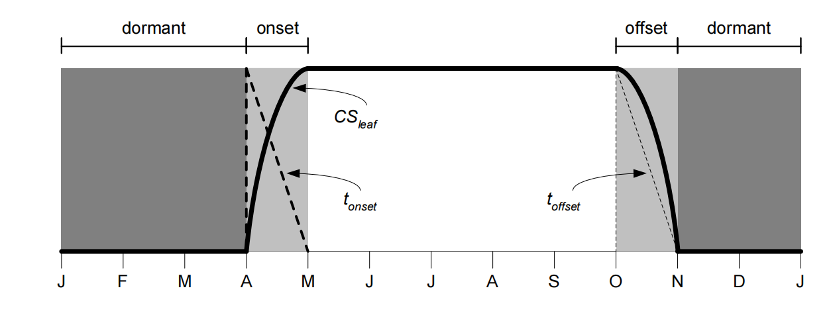
\includegraphics{Figures/植被生物地球化学循环过程/CoLM物候示意图.png}
        \caption{CoLM物候示意图~\citep{lawrence2018} }
        \label{fig:CoLM物候示意图}
      \end{figure}
    }

  \item 活茎周转\\
    CoLM物候模块中,在活茎的周转过程中,活茎细胞或活粗根最终死亡后变成死茎库或死粗根库的组成部分,
    因此,活茎或活粗根碳每年固定比例($r_{\mathrm{lwt}}$)进入死茎库或死粗根库:
    \begin{equation}
      CF_{\mathrm{ {ls\rightarrow ds }}} = CS_{\mathrm{ {ls,t }}} r_{\mathrm{lwt}}
    \end{equation}
    \begin{equation}
      CF_{\mathrm{ {lr\rightarrow dr }}} = CS_{\mathrm{ {lr,t }}} r_{\mathrm{lwt}}
    \end{equation}
    其中,$CF_{\mathrm{ls\rightarrow ds}}$ 是活茎死亡变成死茎的碳通量,
    $CF_{\mathrm{lr\rightarrow dr}}$ 是活粗根死亡变成死粗根的碳通量。活茎和活粗根的周转时间$\tau_{\mathrm{lwt}}$是0.7年:
    \begin{equation}
      \tau_{\mathrm{lwt}} = \frac{0.7}{365 \cdot 86400}
    \end{equation}
    对应的氮通量为:
    \begin{equation}
      NF_{\mathrm{ls\rightarrow ds}} = CS_{\mathrm{ls,t}} \tau_{\mathrm{lwt}} / CN_{\mathrm{dw}}
    \end{equation}
    \begin{equation}
      NF_{\mathrm{lr\rightarrow dr}} = CS_{\mathrm{lr,t}} \tau_{\mathrm{lwt}} / CN_{\mathrm{dw}}
    \end{equation}
    其中,$NF_{\mathrm{ls\rightarrow ds}}$ 是活茎死亡变成死茎的氮,
    $NF_{\mathrm{lr\rightarrow dr}}$ 是活粗根死亡变成死粗根的氮,$CN_{\mathrm{dw}}$ 是死茎和死粗根的碳氮比。

    由于活茎和活粗根的碳氮比低于死茎和死粗根的碳氮比,所以从活茎或活粗根到死茎或死粗根的氮将会有一部分结余,存入植被再利用氮库:
    \begin{equation}
      NF_{\mathrm{{ls\rightarrow rt}}}=\left(\frac{CF_{\mathrm{{ls\rightarrow ds}}}}{CN_{\mathrm{lw}}}\right)-NF_{\mathrm{{ls\rightarrow ds}}}
    \end{equation}
    \begin{equation}
      NF_{\mathrm{{lr\rightarrow rt}}}=\left(\frac{CF_{\mathrm{{lr\rightarrow dr}}}}{CN_{\mathrm{lw}}}\right)-NF_{\mathrm{{lr\rightarrow dr}}}
    \end{equation}
    其中,$NF_{\mathrm{ls\rightarrow rt}}$ 是活茎死亡时回收再利用的氮,$NF_{\mathrm{lr\rightarrow rt}}$ 是活粗根死亡时回收再利用的氮。

\end{enumerate}


\subsection{常绿植被的物候}\label{常绿植被的物候}
常绿植被功能型假设光合作用的净碳收入以及从土壤中的氮摄取直接分配给叶、细根、活茎和活粗茎的组织库。
代表非结构碳库的存储库和传输库将不会有任何碳存储。常绿植被功能型不存在特别的发芽展叶期和落叶期,
叶碳储量存在不随时间变化的固定碳周转速率:
\begin{equation}
  \tau_{\mathrm{bglf}}=\frac{1}{\tau_{\mathrm{lf}} \cdot 365 \cdot 86400}
\end{equation}\todo{可以对$\tau_{\rm lf}$进行说明,下面$r_*$同。}
因此,叶面积指数的季节变化将主要由光合作用净碳收入的季节变化引起。
叶和细根由于物候过程的碳凋落通量($CFP_{\mathrm{lf\rightarrow exit,pft}}$,$CFP_{\mathrm{fr\rightarrow exit,pft}}$)为:
\begin{equation}
  CFP_{\mathrm{lf\rightarrow exit,pft}}=r_{\mathrm{bglf}} CS_{\mathrm{lf,t}}
\end{equation}
\begin{equation}
  CFP_{\mathrm{fr\rightarrow exit,pft}}=r_{\mathrm{bglf}} CS_{\mathrm{fr,t}}
\end{equation}
相应的叶氮凋落通量($NFP_{\mathrm{lf\rightarrow exit,pft}}$)、细根氮凋落通量($NFP_{\mathrm{fr\rightarrow exit,pft}}$)和再利用氮通量($NF_{\mathrm{lf,t\rightarrow rt}}$)为:
\begin{equation}
  N FP_{\mathrm{lf\rightarrow exit,pft}}=CFP_{\mathrm{lf\rightarrow exit,pft}} / CN_{\mathrm{lf}}
\end{equation}
\begin{equation}
  N FP_{\mathrm{fr\rightarrow exit,pft}}=CFP_{\mathrm{fr\rightarrow exit,pft}} / CN_{\mathrm{fr}}
\end{equation}
\begin{equation}
  N F_{\mathrm{lf\rightarrow rt}}=\frac{CFP_{\mathrm{lf\rightarrow exit,pft }}}{CN_{\mathrm{lf}}}-NFP_{\mathrm{lf\rightarrow exit,pft}}
\end{equation}


\subsection{季节落叶植被的物候}\label{季节落叶植被的物候}
季节落叶植被功能型根据积温计算植被物候的发芽展叶期和落叶期,CoLM定义季节性落叶植被功能型仅存在于纬度大于19.5\textdegree 非赤道区域。
季节性落叶植被功能型假设植被每年仅存在一次发芽展叶期和落叶期。由于南北半球冬夏反季,
所以,通过白昼时长的变化判断冬季转变节点,积温(${\mathrm {GDD}}$)的计算在冬季转变节点开始累积\citep{white1997continental}:
\begin{equation}
  {\rm GDD} _{\mathrm{sum}}^{n}=\begin{cases}
    {\rm GDD} _{\mathrm{sum}}^{n-1}+T_{3} \cdot \Delta t \cdot 86400 & T_{3} \geqslant \text{0 \textcelsius} \\
    {\rm GDD} _{\mathrm{sum}}^{n-1} & T_{3}< \text{0 \textcelsius}
  \end{cases}
\end{equation}
其中$GDD_{\mathrm{sum}}^n$是第$n$天后的积温,积温通过对高于0 \textcelsius 的第三层土壤温度 $T_{3}$ (\textcelsius) 进行累加。
当$GDD_{\mathrm{sum}}^n>{\rm GDD}_{\mathrm{sum\_{crit}}}$时,季节性落叶树开始发芽展叶期。${\rm GDD}_{\mathrm{sum\_{crit}}}$ 为发芽物候关键参量,
与前一年的温度 $T_{2m,ann\_{\mathrm{avg}}}$ (\textcelsius)有关:
\begin{equation}
  {\rm GDD}_{\mathrm{sum\_{crit}}}=\exp \left(4.8+0.13 \cdot T_{2 m, ann\_{\mathrm{avg}}}\right)
\end{equation}
当发芽展叶期开始时,积温${\rm GDD}_{\mathrm{sum}}$重设为0,发芽展叶期倒计时重设:
\begin{equation}
  t_{\mathrm{onset}}=86400 \cdot n_{\mathrm{days\_on}}
\end{equation}
其中$n_{\mathrm{days\_on}}=30$,代表发芽展叶期倒计时30天。
同时,发芽展叶期开始的第一个时间步长 $\Delta t$ 内,各营养器官50\% 的存储库($CS_{\mathrm{org,{s}}}$)中的碳进入传输库($CS_{\mathrm{org,{x}}}$),在公式\eqref{CFs_to_x}和\eqref{NFs_to_x}中,${\mathrm {org}}$ 分别代表叶、细根、活茎、死茎、活粗根,死粗根和生长呼吸存储库,即$\text{org=lf}$, ${\mathrm {fr}}$, ${\mathrm {ls}}$, ${\mathrm {ds}}$, ${\mathrm {lr}}$, ${\mathrm {dr}}$和$\mathrm{gresp\_stor}$):
\begin{equation}\label{CFs_to_x}
  CF_{\mathrm{org,{s}}\rightarrow {x}} = 0.5 CS_{\mathrm{org,{s}}}/\Delta t
\end{equation}
同时相应的氮传输同样存在存储库的初期转移:
\begin{equation}\label{NFs_to_x}
  NF_{\mathrm{org,{s}}\rightarrow {x}} = 0.5  NS_{\mathrm{org,{s}}}/\Delta t
\end{equation}

如果到夏天,日照长度缩短时还未开始发芽展叶期,
$GDD_{\mathrm{sum}}^n$ 重设为0直至冬天。当发芽展叶期开始后,30天倒计时开始,直至 $t_{\mathrm{onset}}=0$,发芽展叶期结束:
%
\begin{equation}
  t_{\mathrm{onset}}^n=t_{\mathrm{onset}}^{n-1}-\Delta t
\end{equation}
当日照长度低于39300秒时,植被进入落叶期,落叶期倒计时为15天:
\begin{equation}
  t_{\mathrm{offset}}^n=t_{\mathrm{offset}}^{n-1}-\Delta t
\end{equation}


\subsection{胁迫落叶植被的物候}

胁迫落叶植被功能型包括草地和热带干旱落叶树等可以既响应干旱又响应温度胁迫。
当胁迫不存在时,该植被类型的物候还可以转变为常绿树的物候。当胁迫触发时,传输库的碳很快转变为组织库的碳。


当温度暖和,干旱成为触发胁迫的主要条件。当上一次落叶期结束后,土壤水分因子$SWI$就开始从0累加:
\begin{equation}
  SWI_{\mathrm{sum}}^{n}=\left\{\begin{array}{ll}SWI_{\mathrm{sum}}^{n-1}+f_{\mathrm{d a y}} & \text{ 当 }\ \psi_{\mathrm{s, 3}} \geqslant -0.6\ \mathrm{MPa} \\
      SWI_{\mathrm{sum}}^{n} &  \text{ 当 }\ \psi_{\mathrm{s, 3}}<-0.6\ \mathrm{MPa}
  \end{array}\right.
\end{equation}
其中$SWI_{\mathrm{sum}}^n$代表土壤水分因子累加到第$n$个时间步长,$\psi_{\mathrm{s,3}}$是第三层土壤的水势,当土壤水势高于 -0.6 MPa 时,土壤足够湿润,土壤水分因子就开始累加,$f_{\mathrm{d a y}}$是模拟时间步长,单位:天。
当土壤水分因子高于15,同时过去十天有至少 20 mm 的降水,并且冷温胁迫没有触发,日照时长超过6小时,植被进入发芽展叶期。


同时,因为土壤温度过低 ($FD_{\mathrm{sum}}^n>15$),需要应用冷气候标准
\begin{equation}
  FD_{\mathrm{sum}}^{n}=\left\{\begin{array}{ll}FD_{\mathrm{sum}}^{n-1}+f_{\mathrm{day}} &  \text{ 当 }\ T_{3} > \text{0 \textcelsius} \\
      FD_{\mathrm{sum}}^{n-1} &  \text{ 当 }\ T_{3} \leqslant \text{0 \textcelsius}
  \end{array}\right.
\end{equation}
即当气温低,发芽展叶期的触发需要土壤温度和土壤湿度同时满足条件:
$SWI_{\mathrm{sum}}>15,\ GDD_{\mathrm{sum}}>GDD_{\mathrm{sum\_crit}}$,和日照时长大于6小时。
当发芽展叶期开始后,30天倒计时开始,直至$t_{\mathrm{onset}}=0$,发芽展叶期结束:
\begin{equation}
  t_{\mathrm{o n s e t}}^{n}=t_{\mathrm{o n s e t}}^{n-1}-\Delta t
\end{equation}
当持续土壤干旱或持续低温或日照长度低于6小时,胁迫落叶期就将触发。
土壤干旱用累积落叶土壤水分因子($OSWI_{\mathrm{sum}}^n$)来量化:
\begin{equation}
  OSWI_{\mathrm{sum}}^{n}=\left\{\begin{array}{ll}OSWI_{\mathrm{sum}}^{n-1}+f_{\mathrm{d a y}}, &  \text{ 当 }\ \psi_{\mathrm{s, 3}}<-2\ \mathrm{MPa} \\
      \max \left(OSWI_{\mathrm{sum}}^{n-1}-f_{\mathrm{d a y}},\ 0\right) &  \text{ 当 }\ \psi_{\mathrm{s, 3}}>-2\ \mathrm{MPa}
  \end{array}\right.
\end{equation}
当前面一个发芽展叶期已经完成时,且$OSWI_{\mathrm{sum}}^n\geqslant 15$,即触发落叶期。
冷温胁迫用累积落叶冷冻天数来量化:
\begin{equation}
  OFD_{\mathrm{sum}}^{n}=\left\{\begin{array}{ll}OFD_{\mathrm{sum}}^{n-1}+f_{\mathrm{d a y}} &  \text{ 当 }\ {T}_{\mathrm{s, 3}} \leqslant \text{0 \textcelsius} \\
  \max \left(OFD_{\mathrm{sum}}^{n-1}-f_{\mathrm{d a y}}, 0\right) & \text{ 当 }\ {T}_{\mathrm{s, 3}}> \text{0 \textcelsius}\end{array}\right.
\end{equation}
当前面一个发芽展叶期已经完成时,且$OFD_{\mathrm{sum}}^n\geq15$,即触发落叶期。


总而言之,当以上三个条件($OSWI_{\mathrm{sum}}^n\geqslant 15$,$OFD_{\mathrm{sum}}^n\geqslant 15$,日照时长小于6小时)满足其一,植被进入落叶期,落叶期倒计时为15天:
\begin{equation}
  t_{\mathrm{offset}}^{n}=t_{\mathrm{offset}}^{n-1}-\Delta t
\end{equation}
当落叶条件始终不满足(1年以上),胁迫落叶植被功能型就表现为常绿物候。
长生长季控制变量(${\mathrm {LGS}}$)被用来刻画该常绿物候的周转速率:
\begin{equation}
  \tau_{\mathrm{b g l f}}=\frac{L G S}{\tau_{\mathrm{lf}} \cdot 365 \cdot 86400}
\end{equation}

\begin{equation}
  L G S=\begin{cases}
    0 &  \text{ 当 }\ n_{\mathrm{ {days}}\_{\mathrm{active}}}<365 \\
    \frac{n_{\mathrm{ {days\_{active}}}}}{365}-1 &  \text{ 当 }\ 365 \leqslant n_{\mathrm{ {days }}\_{\mathrm{active}} }<730 \\
    1 & \text{ 当 }\ n_{\mathrm{ {days}}\_{\mathrm{active}}} \geqslant 730
  \end{cases}
\end{equation}
$n_{\mathrm{days\_{active}}}$ 是植被只从上次发芽开始的天数。


发芽展叶期的每个时间步长,各个器官都有储存库的碳进入传输库,其传输速率为$CF_{\mathrm{org,{s}}\rightarrow {x}}$,在公式\eqref{CFs_to_x_str},\eqref{CFx_to_t_str},\eqref{NFs_to_x_str}和\eqref{NFx_to_t_str}中,${\mathrm {org}}$代表叶,细根,活茎,死茎,活粗根和死粗根,即$\text{org=lf}$, ${\mathrm {fr}}$, ${\mathrm {ls}}$, ${\mathrm {ds}}$, ${\mathrm {lr}}$和${\mathrm {dr}}$:
\begin{equation}\label{CFs_to_x_str}
  CF_{\mathrm{org,{s}\rightarrow {x}}}=CS_{\mathrm{org,{s}} }\cdot \tau_{\mathrm{bgtr}}
\end{equation}
同时传输库碳全部进入组织库,其速率为$CF_{\mathrm{org,{x} \rightarrow {t}}}$:
\begin{equation}\label{CFx_to_t_str}
  CF_{\mathrm{org,{x}\rightarrow {t}}}=CS_{\mathrm{org,{x}}}/\Delta t
\end{equation}
对应的氮同样有从存储库到转移库的过程,其速率为$NF_{\mathrm{org,{s}\rightarrow {x}}}$:
\begin{equation}\label{NFs_to_x_str}
  NF_{\mathrm{org,{s}\rightarrow {x}}}=NS_{\mathrm{org,{s}}}\cdot\tau_{\mathrm{bgtr}}
\end{equation}
传输库氮再全部进入组织库,其速率为:$NF_{\mathrm{org,{x} \rightarrow {t}}}$
\begin{equation}\label{NFx_to_t_str}
  NF_{\mathrm{org,{x}\rightarrow {t}}}=NS_{\mathrm{org,{x}}}/\Delta t
\end{equation}


\subsection{物候凋落物}\label{物候凋落物}
物候的凋落物主要来源于叶和细根的组织结构库,其中叶和细根凋落物都将进入代谢凋落物、
纤维素凋落物和木质素凋落物,其速率为$CF\_P_{\mathrm{org,t\rightarrow lit,pat}}$,其中,${\mathrm {CFP}}$指物候过程引起生态系统碳传输,${\mathrm {org}}$是指凋落过程来源于植物的器官,在公式\eqref{CFpfttopat}和\eqref{NFpfttopat}中,特指叶和细根($\text{org=lf}$或${\mathrm {fr}}$),存储碳库假设在物候凋落前已回收,${\mathrm {lit}}$代表掉落过程的传输目的地,即三个凋落物库,在公式\eqref{CFpfttopat}和\eqref{NFpfttopat}中,代谢凋落物,纤维素凋落物和木质素凋落物($\text{lit=met}$,${\mathrm {cel}}$ 和${\mathrm {lig}}$),${\mathrm {pat}}$指patch尺度上的变量,即多个pft的均值或总和,${\mathrm {pft}}$指该通量基于植被功能型尺度:
\begin{equation}\label{CFpfttopat}
  CFP_{\mathrm{org,t\rightarrow lit,pat}}=\sum_{\mathrm{pft=0}}^{npft}{CFP_{\mathrm{org,t \rightarrow exit,pft}}\cdot f_{\mathrm{{org\rightarrow lit},pft}}\cdot{wcol_{\mathrm{pft}}}}
\end{equation}
其中$f_{\mathrm{org\rightarrow lit}}$是叶片和细根凋落物中,代谢凋落物,纤维素和木质素凋落物所占得比例,${wcol_{\mathrm{pft}}}$ 代表每个植被功能型的面积权重。

对应的物候过程引起的氮凋落也是从叶和细根的结构组织库传入三个凋落物氮库中,其速率$NFP_{\mathrm{org,t\rightarrow lit,pat}}$在patch上的平均值可表达为:
\begin{equation}\label{NFpfttopat}
  NFP_{\mathrm{org,t\rightarrow lit,pat}}=\sum_{\mathrm{pft=0}}^{npft}{NFP_{\mathrm{org,t \rightarrow exit,pft}}\cdot f_{\mathrm {org \rightarrow lit,pft}}\cdot {wcol_{\mathrm{pft}}}}
\end{equation}
$NFP_{\mathrm{org,t \rightarrow exit,pft}}$代表pft尺度因物候凋落过程离开叶或细根组织结构库的氮速率。

\subsection{植被的自然死亡}\label{植被的自然死亡}
植被的整体自然死亡率被假设为2\%每年。
所有的叶、细根、活茎、死茎、或粗根和死粗根的组织库、存储库和传输库的凋落速率受死亡率的控制,
其凋落物碳氮通量为$CFM_{\mathrm{org,pool\rightarrow exit,pft}}$和$NF_{\mathrm{org,pool\rightarrow exit,pft}}$, 在公式\eqref{CFMexit},\eqref{NFMexit}中,${\mathrm {org}}$是指凋落物来源于某个植物器官,即叶,细根,活茎,死茎,活粗根和死粗根,即$\text{org=lf}$, ${\mathrm {fr}}$, ${\mathrm {ls}}$, ${\mathrm {ds}}$, ${\mathrm {lr}}$和${\mathrm {dr}}$,${\mathrm {pool}}$指凋落物来源于植物器官的子库,即组织结构库,存储库和临时传输库,即$\text{pool=t}$,${\mathrm {s}}$和${\mathrm {x}}$:

\begin{equation}\label{CFMexit}
  CFM_{\mathrm{org,pool\rightarrow exit,pft}}=CS_{\mathrm{org,pool}}\cdot \frac{0.2\%}{365\cdot 86400}
\end{equation}

\begin{equation}\label{NFMexit}
  NFM_{\mathrm{org,pool\rightarrow exit,pft}}=NS_{\mathrm{org,pool}}\cdot \frac{0.2\%}{365\cdot 86400}
\end{equation}

死亡的植被的叶和细根的碳氮通量将进入不同凋落物库,通过对patch内的所有pft尺度通量加权求和,得到patch尺度的碳氮通量$CFM_{\mathrm{org,t\rightarrow lit,pat}}$,$NFM_{\mathrm{org,t\rightarrow lit,pat}}$,在公式\eqref{CFMt_to_lit}和\eqref{NFMt_to_lit}中,${\mathrm {org}}$代表叶和细根,即$\text{org=lf}$, ${\mathrm {fr}}$。${\mathrm {lit}}$是不同的凋落物库,包括代谢凋落物,纤维素凋落物和木质素凋落物,即$\text{lit=met}$, ${\mathrm {cel}}$和${\mathrm {lig}}$:
\begin{equation}\label{CFMt_to_lit}
  CFM_{\mathrm{org,t\rightarrow lit,pat}}=\sum_{\mathrm{pft=0}}^{npft}{CFM_{\mathrm{org,t\rightarrow exit,pft}}\cdot f_{\mathrm{{org}\rightarrow lit,pft}}\cdot{wcol_{\mathrm{pft}}}}
\end{equation}
\begin{equation}\label{NFMt_to_lit}
  NFM_{\mathrm{org,t\rightarrow lit,pat}}=\sum_{\mathrm{pft=0}}^{npft}{NFM_{\mathrm{org,t\rightarrow exit,pft}}\cdot f_{\mathrm{{org}\rightarrow lit,pft}}\cdot{wcol_{\mathrm{pft}}}}
\end{equation}
其中$f_{\mathrm{org\rightarrow lit,pft}}$是不同植被器官凋落物进入不同凋落物库的比例,${wcol_{\mathrm{pft}}}$ 代表每个植被功能型pft的面积比。


活茎、死茎、活粗根和死粗根在树木死亡后进入木质部残体库,通过对patch内的所有pft尺度通量加权求和,得到patch尺度的碳氮通量$CFM_{\mathrm{org,t\rightarrow cwd,pat}}$和$NFM_{\mathrm{org,t\rightarrow cwd,pat}}$,在公式\eqref{CFMt_to_cwd}和\eqref{NFMt_to_cwd}中,${\mathrm {org}}$代表活茎、死茎、活粗根和死粗根,即$\text{org=ls}$, ${\mathrm {ds}}$, ${\mathrm {lr}}$和${\mathrm {dr}}$:
\begin{equation}\label{CFMt_to_cwd}
  CFM_{\mathrm{org,t\rightarrow cwd,pat}}=\sum_{\mathrm{pft=0}}^{npft}{CFM_{\mathrm{org,t\rightarrow exit,pft}}\cdot {wcol_{\mathrm{pft}}}}
\end{equation}
\begin{equation}\label{NFMt_to_cwd}
  NFM_{\mathrm{org,t\rightarrow cwd,pat}}=\sum_{\mathrm{pft=0}}^{npft}{NFM_{\mathrm{org,t\rightarrow exit,pft}}\cdot {wcol_{\mathrm{pft}}}}
\end{equation}

此外,所有的含有非结构储存库和传输库在植被死亡后都进入代谢凋落物库中,通过对patch内的所有pft尺度通量加权求和,得到patch尺度的碳氮通量$CFM_{\mathrm{org,{s}\rightarrow met,pat}}$和$CFM_{\mathrm{org,x\rightarrow met,pat}}$为所有所有植被功能型的总和,在公式~\eqref{CFMs_to_met},\eqref{CFMx_to_met},\eqref{NFMs_to_met} 和~\eqref{NFMx_to_met} 中,${\mathrm {org}}$代表所有6种植被器官,即$\text{org=lf}$, ${\mathrm {fr}}$, ${\mathrm {ls}}$, ${\mathrm {ds}}$, ${\mathrm {lr}}$和${\mathrm {dr}}$:
\begin{equation}\label{CFMs_to_met}
  CFM_{\mathrm{org,{s}\rightarrow met,pat}}=\sum_{\mathrm{pft=0}}^{npft}{CFM_{\mathrm{org,{s}\rightarrow exit,pft}}\cdot{wcol_{\mathrm{pft}}}}
\end{equation}
\begin{equation}\label{CFMx_to_met}
  CFM_{\mathrm{org,{x}\rightarrow met,pat}}=\sum_{\mathrm{pft=0}}^{npft}{CFM_{\mathrm{org,{x}\rightarrow exit,pft}}\cdot{wcol_{\mathrm{pft}}}}
\end{equation}

对应的氮通量中,植被死亡后,除了存储库和传输库的凋落物将进入代谢凋落物库,再利用氮库也进入代谢凋落物库:
\begin{equation}\label{NFMs_to_met}
  NFM_{\mathrm{org,{s}\rightarrow met,pat}}=\sum_{\mathrm{pft=0}}^{npft}{NFM_{\mathrm{org,{s}\rightarrow exit,pft}}\cdot{wcol_{\mathrm{pft}}}}
\end{equation}
\begin{equation}\label{NFMx_to_met}
  NF_{\mathrm{org,{x}\rightarrow met,pat}}=\sum_{\mathrm{pft=0}}^{npft}{NFM_{\mathrm{org,{x}\rightarrow exit,pft}}\cdot{wcol_{\mathrm {p}} }}
\end{equation}
\begin{equation}
  NF_{\mathrm{rt\rightarrow met,pat}}=\sum_{\mathrm{pft=0}}^{npft}{NFM_{\mathrm{rt\rightarrow exit,pft}}\cdot{wcol_{\mathrm{pft}}}}
\end{equation}

\chapter{土壤凋落物生物地球化学循环过程}\label{土壤凋落物生物地球化学循环过程}
\echapter{Soil Litter Biogeochemical Cycles}
%\addcontentsline{toc}{chapter}{土壤凋落物生物地球化学循环过程}
\begin{mymdframed}{代码}
  本章对应代码源文件位于\texttt{main/BGC/}目录下。
\end{mymdframed}

%\begin{土壤凋落物生物地球化学循环过程}
植被物候和自然死亡凋落的植被碳进入土壤凋落物库后进行进一步碳氮循环。在土壤中凋落物碳氮元素经过土壤分解,
垂直混合后。土壤碳通过土壤呼吸回到大气,土壤氮通过矿化作用进入土壤无机氮库,然后被植被吸收或进一步固定在土壤有机氮库中。

CoLM的土壤和凋落物存在垂直分层结构,碳氮动态变化根据平衡方程在每一层分别积分:
\begin{equation}
  \begin{aligned}
    \frac{\partial C_{i}(z)}{\partial t}=R_{i}(z) &+\sum_{i \neq j}\left(1-r f_{j}\right) T_{j i} k_{j}(z) C_{j}(z)-k_{i}(z) C_{i}(z) \\
    &+\frac{\partial}{\partial z}\left(D(z) \frac{\partial C_{i}}{\partial z}\right)+\frac{\partial}{\partial z}\left[A(z) C_{i}(z)\right]
  \end{aligned}
\end{equation}
其中,$C_i\left(z\right)$是第$z$层的土壤碳密度(\unit{g.C.m^{-3}}); $R_i (z)$ 是第 $z$ 层土壤的凋落物碳输入,
$\sum_{i\neq j}{\left(1-{rf}_j\right)T_{ji}k_j\left(z\right)C_j\left(z\right)}$代表土壤碳库$j$到碳库$i$的碳转变;
$k_j\left(z\right)$是第$z$层碳库$j$的周转速率;${rf}_j$是$j$库在转换中呼吸掉的碳的比例;
$\left(1-{rf}_j\right)$是微生物对库$j$分解的碳利用效率,$T_{ji}$是碳转换途径$j$到$i$在所有离开$j$库碳通量
(不包括因呼吸作用离开$j$库)的比例;$k_i\left(z\right)C_i\left(z\right)$代表库$i$的碳分解;
$\frac{\partial}{\partial z}\left(D\left(z\right)\frac{\partial C_i}{\partial z}\right)+\frac{\partial}{\partial z}\left(A\left(z\right)C_i\left(z\right)\right)$代表碳垂直传输。


\section{土壤凋落物分解}\label{土壤凋落物分解}
\esection{Soil Litter Decomposition}

\begin{mymdframed}{代码}
  本节对应的代码文件为\texttt{MOD\_BGC\_Soil\_BiogeochemDecompCascadeBGC.F90}。
\end{mymdframed}

土壤凋落物碳氮分解在每一层分别进行,分解速率受每一层不同的环境因子控制:
\begin{equation}
  k_{i}(z)=k_{\mathrm{base},i} \cdot \xi_{\mathrm{tsoil}}(z) \cdot \xi_{\mathrm{water}}(z) \cdot \xi_{\mathrm{depth}}(z)
\end{equation}
其中$k_{\mathrm{base},i}$是库$i$的基础周转速率,$\xi_{\mathrm{tsoil}}$是温度环境因子,$\xi_{\mathrm{water}}$是土壤水环境因子,$\xi_{\mathrm{depth}}$是深度因子。


\section{环境限制因子}\label{环境限制因子}
\esection{Environmental Constraints}

\begin{mymdframed}{代码}
  本节对应的代码文件为\texttt{MOD\_BGC\_Soil\_BiogeochemDecompCascadeBGC.F90}。
\end{mymdframed}

CoLM生物地球化学模块,控制土壤分解的环境因子包括土壤温度因子,土壤水分因子和深度因子。其中土壤温度因子运用$Q_{10}$关系:
\begin{equation}
  \xi_{\mathrm{t s o i l}}(z)=Q_{10}^{\frac{T_{\mathrm{{soil }}}(z)-273.15-25}{10}}
\end{equation}
其中,$\xi_{\mathrm{tsoil}}\left(z\right)$是第$z$层的土壤温度因子;$T\left(z\right)$是第$z$层的土壤温度 (K),$Q_{10}$是温度敏感性参数。


当土壤温度低于0 \textcelsius,土壤完全结冰,土壤分解速率迅速下降。土壤温度因子使用另一个关系:
\begin{equation}
  \xi_{\mathrm{t s o i l}}(z)=Q_{10}^{-2.5} \cdot 1.5^{\frac{T_{\mathrm{{soil }}}(z)-273.15}{10}}
\end{equation}
土壤水分因子根据土壤水势的计算而得出,刻画土壤水分对土壤分解的影响:
\begin{equation}
  \xi_{\mathrm{w a t e r}}(z)=\begin{cases}
    \frac{\log \left(\frac{\psi_{\min }}{\psi(z)}\right)}{\log \left(\frac{\psi_{\min }}{\psi_{\max }}\right)}
    & \psi(\mathrm{z})>\psi_{\min } \\
    0  & \psi(z)<\psi_{\min }
  \end{cases}
\end{equation}
其中,$\xi_{\mathrm{water}}\left(z\right)$是第$z$层的土壤水分因子,$\psi\left(z\right)$是第$z$层的土壤水势,
$\psi_{\mathrm{min}}$是最小土壤水势,$\psi_{\mathrm{max}}$是最大土壤水势。当土壤水势小于最小土壤水势时,土壤周转速率为0。


深度因子参数化了影响土壤分解的一些其他环境因素,比如,微生物过程、矿化表面或聚合稳定等过程~\citep{koven2013effect},
是拟合碳垂直浓度剖面的重要因素~\citep{jenkinson2008turnover}:
\begin{equation}
  \xi_{\mathrm{d e p t h}}={\mathrm e}^{-\frac{z_{\mathrm{i}}}{10}}
\end{equation}
其中$z_{\mathrm{i}}$是土壤第z层的节点深度(m)。


\subsection{土壤分解的氮限制}\label{土壤分解的氮限制}
\esubsection{Nitrogen Limitation}
\begin{mymdframed}{代码}
  本节对应的代码文件为\\ \texttt{MOD\_BGC\_Soil\_BiogeochemPotential.F90}\\
  \texttt{MOD\_BGC\_Soil\_BiogeochemDecomp.F90}。
\end{mymdframed}

土壤分解速率同样会受到土壤中无机氮含量的限制,但量化氮限制对土壤分解速率的影响,需要先计算无氮限制条件下的潜在土壤分解($CF_{pot,i}$),其中土壤/凋落物库$i$ (第$z$层) 的潜在土壤分解为:
\begin{equation}
  C F_{\mathrm{pot},i}(z)=C_{i}(z) k_{i}(z)
\end{equation}
从库$i$到库$j$的碳传输通量(第$z$层)为:
\begin{equation}
  C F_{\mathrm{pot}, i \rightarrow j}=C_{i}(z) k_{i}(z) \cdot\left(1-r f_{i}\right) \cdot T_{i j}
\end{equation}
相应的从库$i$到库$j$的传输中,$r f_{i}$和$T_{i j}$的定义在本章开始位置介绍,潜在的净无机氮增加($NF_{\mathrm{pot\_min,}i\gets j}$)等于矿化作用引起的无机氮增加(等式右边第一项)减去有机氮固定引起的无机氮减少(等式右边第二项):
\begin{equation}
  \begin{aligned}
    NF_{\mathrm{pot\_min}, i \rightarrow j}\left(z\right)&=\frac{C_{i}(z) k_{i}(z) \cdot T_{ij}}{C N_{i}}-\frac{C F_{\mathrm{pot}, i \rightarrow j}}{C N_{j}} \\
    & =\frac{C_{i}(z) k_{i}(z) \cdot T_{i j} \cdot \frac{C N_{j}}{C N_{i}}-C_{i}(z) k_{i}(z) \cdot T_{i j} \cdot\left(1-r f_{i}\right)}{C N_{j}} \\
    &=-\frac{C_{i}(z) k_{i}(z) T_{i j}\left(1-r f_{i}-\frac{C N_{j}}{C N_{i}}\right)}{C N_{j}}
  \end{aligned}
\end{equation}
$C N_{j}$代表第$j$个库的碳氮比,
如图~\ref{fig:CoLM土壤凋落物碳氮循环网络示意图} 所示共有10个土壤/凋落物之间的碳氮传输路径,所有10个传输路径引起的潜在净无机氮增加可具体表示为:
\begin{equation}\label{NF_pot_minmet}
  NF_{\mathrm{{pot}\_{min,i \rightarrow {j}}}}(z)=-\frac{C_{\mathrm{{i}}}(z) k_{\mathrm{{i}}}(z) T_{\mathrm{i, j}}\left(1-r f_{\mathrm{i}}-\frac{C N_{\mathrm{{j }}}}{C N_{\mathrm{i}}}\right)}{C N_{\mathrm{{j }}}}
\end{equation}

其中$\mathrm {i \rightarrow j}$包括10个传输路径,把所有传输公式~\eqref{NF_pot_minmet}所有正项求和,得到总固化作用在每层土壤中对无机氮的潜在需求$NF_{\mathrm{pot\_id,vr}}(z)$,其中下标id代表immobalization demand,vr代表vertical resolved:
\begin{equation}\label{NF_immob_demand_vr}
  NF_{\mathrm{pot\_id,vr}}(z)=-\sum_{k=1}^{10}\min{\left(NF_{\mathrm{pot\_min},i(k)\rightarrow j(k)}\left(z\right), 0\right)}
\end{equation}
把每层土壤的固化作用所需要的无机氮的潜在需求加在一起得到总的土壤微生物固化作用需要的氮:
\begin{equation}
    NF_{\mathrm{pot\_id}}=\sum_{z=1}^{10}{NF_{\mathrm{pot\_id,vr}}(z) \cdot \Delta z}
\end{equation}
当总固化作用需要的无机氮 ($NF_{\mathrm{pot\_id}}$) 大于土壤中可以提供的无机氮时,某个传输量就将减小,土壤分解就将减慢。


\section{植被土壤的氮竞争}\label{植被土壤的氮竞争}
\esection{Soil Nitrogen Competition}
\begin{mymdframed}{代码}
  本节对应的代码文件为\texttt{MOD\_BGC\_Soil\_BiogeochemCompetition.F90}。
\end{mymdframed}

实际上,土壤分解可以利用的无机氮往往比土壤中存在的无机氮还要小,因为土壤微生物利用无机氮还需要和植被进行竞争。

植被潜在氮需求 ($NF_{\mathrm{pot\_{pd}}}$) 在公式 \eqref{NF_plant_demand_soil} 中已经被完整计算,若植被氮需求和土壤微生物固氮需求 ($NF_{\mathrm{pot\_{id}}}$) 小于总土壤无机氮含量(${NS}_{\mathrm{sminn}}$):
\begin{equation}
  \left(NF_{\mathrm{pot\_{pd}}}+NF_{\mathrm{pot\_id}}\right)\cdot\Delta t<NS_{\mathrm{sminn}}
\end{equation}
则土壤无机氮含量充分,不存在氮限制,反之则需要计算氮限制。

CoLM将植被的潜在氮需求($NF_{\mathrm{pot\_{pd}}}$) 按无机氮含量的垂直分布比例分摊给每层土壤:
\begin{equation}
  NF_{\mathrm{pot\_{pd},vr}}(z)=NF_{\mathrm{pot\_{pd}}}\cdot\frac{NS_{\mathrm{sminn,vr}}(z)}{NS_{\mathrm{sminn}}}
\end{equation}
结合公式 \eqref{NF_pot_minmet}--\eqref{NF_immob_demand_vr} 计算土壤氮固化作用的需求,可以得出每层土壤无机氮的总需求($NF_{\mathrm{pot\_ipd,vr}}(z)$),下标ipd代表nitrogen demand from soil immobalization and plant uptake
\begin{equation}
  NF_{\mathrm{pot\_ipd,vr}}(z)=NF_{\mathrm{pot\_{pd},vr}}(z)+NF_{\mathrm{pot\_id,vr}}\left(z\right)
\end{equation}
CoLM在每层土壤中分别考虑无机氮的供需关系及其和每层无机氮含量 ${NS}_{\mathrm{sminn,vr}}(z)$ 的关系,
我们得到每层土壤分解的氮限制因子 ($f_{\mathrm{id,vr}}$) 和植被氮吸收的限制因子($f_{\mathrm{pd,vr}}$):
\begin{equation}
  f_{\mathrm{pd,vr}}(z)=f_{\mathrm{id,vr}}(z)=\frac{NS_{\mathrm{sminn,vr}}(z)}{NF_{\mathrm{ipd,vr}}(z)\cdot\Delta t}
\end{equation}
平均土壤各层求得植被氮吸收的限制因子($f_{\mathrm{pd}}$):
\begin{equation}
  f_{\mathrm{pd}}=\frac{\sum_{z=1}^{n=10}{f_{\mathrm{pd,vr}}(z)\cdot NF_{\mathrm{pot\_{pd},vr}}(z)}}{NF_{\mathrm{pot\_{pd}}}}
\end{equation}
实际氮吸收 $(NF_{\mathrm{sminn\_{alloc}}}$) 可以由公式 \eqref{NF_sminn_alloc} 求出,至此,章节~\ref{植被碳氮分配} 的所有变量可解。
实际碳传输,也可根据氮限制因子 ($f_{\mathrm{id,vr}}(z)$) 进一步得出:
\begin{equation}
  CF_{\mathrm{Source \rightarrow { Dest }}}(z)=\left\{\begin{array}{ll}C F_{\mathrm{pot, Source \rightarrow Dest}}(z) \cdot f_{\mathrm{id, vr}}(z) & NF_{\mathrm{pot\_{min}, Source \rightarrow {Dest}}} <0 \\
      CF_{\mathrm{pot, Source \rightarrow { Dest }}}(z) & NF_{\mathrm{pot\_{min}, Source \rightarrow {Dest}}} \geqslant 0
  \end{array}\right.
\end{equation}

每个土壤凋落物碳库在每层土壤的实际碳分解:
\begin{equation}
  CF_{\mathrm{Source}}(z)=\frac{CF_{\mathrm{Source \rightarrow { Dest }}}(z)}{1-r f_{\mathrm{Source}}}
\end{equation}

其中每层土壤的异养呼吸$CF_{\mathrm{hr,vr}}\left(z\right)$:
\begin{equation}
  \begin{aligned}
    C F_{\mathrm{h r, vr}}(z)&=C F_{\mathrm{met, vr}}(z) \cdot r f_{\mathrm{met}}+C F_{\mathrm{cel, vr}}(z) \cdot r f_{\mathrm{cel}}+C F_{\mathrm{lig, vr}}(z) \cdot r f_{\mathrm{lig}} \\
    &+C F_{\mathrm{{soill } 1, vr}}(z) \cdot r f_{\mathrm{{soil1 }}}+C F_{\mathrm{{soil2,vr }}}(z) \cdot r f_{\mathrm{{soil2 }}}+C F_{\mathrm{{soil3,vr }}}(z) \cdot r f_{\mathrm{{soil3 }}}
  \end{aligned}
\end{equation}
同样的,实际氮传输,也根据氮限制因子下降:
\begin{equation}
  CF_{\mathrm{Source \rightarrow Dest}}(z)=\left\{\begin{array}{ll} CF_{\mathrm{pot, Source \rightarrow Dest}}(z) \cdot f_{\mathrm{immob\_demand, vr}}(z) & NF_{\mathrm{pot\_{min, Source \rightarrow Dest}}} <0 \\
      CF_{\mathrm{pot, Source \rightarrow Dest}}(z) & NF_{\mathrm{pot\_{min, Source\rightarrow Dest}}} \geqslant 0
  \end{array}\right.
\end{equation}

实际土壤氮固化作用同样受氮限制因子的影响:
\begin{equation}
  NF_{\mathrm{immob,vr}}(z)=NF_{\mathrm{pot\_id,vr}}(z)\ \cdot\ f_{\mathrm{id,vr}}(z)
\end{equation}
但因为氮矿化作用为土壤提供无机氮,实际的土壤氮矿化作用仍然运用公式~\eqref{NF_immob_demand_vr}。


\section{土壤凋落物的垂直传输}\label{土壤凋落物的垂直传输}
\esection{Vertical Transport of Soil Litter}
\begin{mymdframed}{代码}
  本节对应的代码文件为\texttt{MOD\_BGC\_Soil\_BiogeochemLittVertTransp.F90}。
\end{mymdframed}

土壤凋落物的碳氮循环的垂直结构在章节~\ref{垂直分层结构} 已经被大致介绍。地上凋落物和地下凋落物组成了地下碳循环的输入,存在显著的垂直变化。
此外,土壤碳氮分解存在深度因子的影响,也是影响土壤碳氮模拟垂直分布的重要因子。除此之外,碳氮的垂直混合也是影响土壤碳氮浓度垂直剖面曲线的关键。
CoLM考虑土壤碳氮传输仅存在扩散作用下,和求解土壤湿度的垂直分布解法类似。
详细土壤垂直扩散方程的参数化方案见~\citet{koven2009formation,koven2011permafrost,koven2013effect,koven2015permafrost} 。

\chapter{生物地球化学循环预热加速}\label{生物地球化学循环预热加速}
%\addcontentsline{toc}{chapter}{生物地球化学循环预热加速}
\begin{mymdframed}{代码}
本节对应的代码文件为\texttt{MOD\_BGC\_CNSASU.F90}。
\end{mymdframed}
%\begin{生物地球化学循环预热加速}
生物地球化学循环预热是陆地生态系统碳氮循环模拟必不可少的初始化过程,是众多模式比较计划都采用的标准初始化流程。
生物地球化学循环预热通过重复使用同样的气候强迫场和大气二氧化碳浓度数据,使陆地生态系统碳氮储量达到平衡。
通常来说,不同模型间平衡态碳氮储量的差异往往大于历史时期由于$\rm CO_2$浓度上升引起的碳氮储量变化的不确定性。
因此,生物地球化学循环预热过程十分重要。但由于高纬度地区的低温气候造成土壤分解过慢,
碳氮预热达到平衡态需要上千年的模拟时间,如何加速生物地球化学循环预热过程十分关键。
CoLM生物地球化学循环模块运用半解析预热方法~\citep{xia2012semi}。从碳氮平衡方程入手,求解平衡态的碳氮库大小。


\section{植被生物地球化学循环预热加速}
CoLM植被碳氮循环可以表示为21个碳库和22个氮库的碳氮平衡方程组~\citep{lu2020full},
可以写成矩阵形式:
\begin{equation}
\frac{d C_{veg}}{dt}=B I_{Cin}+\left(A_{p h c}(t) K_{p h c}+A_{gmc}(t) K_{gmc}\right) C_{veg}(t)
\end{equation}
\begin{equation}
\frac{d N_{\text {veg}}}{dt}=B I_{Nin}+\left(A_{phn}(t) K_{phn}+A_{gmn}(t) K_{gmn}\right) N_{\text {veg }}(t)
\end{equation}
$C_{veg}$ 和$N_{veg}$ 是植被碳氮库的状态变量 (\unit{g.C.m^{-2}} 和 \unit{g.N.m^{-2}}),是长度分别为21和22的列向量,
具体内容见章节~\ref{植被碳氮库结构} 对植被碳氮库的详细介绍。$I_{Cin}$ 和$I_{Nin}$ 分别是植被的碳氮输入(\unit{g.C.m^{-2}.s^{-1}} 和 \unit{g.N.m^{-2}.s^{-1}}),
是标量。其中,碳输入来源于净第一性生产力,氮输入来源于生物固氮和植被被动氮吸收。
$B$是分配系数向量,代表植被碳氮输入分配到每个植被碳氮库的比例。  
$K_{phc}$和$K_{gmc}$是21$\times$21的对角矩阵,分别代表植被每个库因为物候过程和自然死亡过程产生的碳周转速率(\unit{s^{-1}})。
$K_{phn}$和$K_{gmn}$是22$\times$22的对角矩阵,分别代表植被每个库因为物候过程和自然死亡过程产生的氮周转速率(\unit{s^{-1}}):
\begin{equation}
K_{p h c}=\left(\begin{array}{ccc}k_{p 1} & \cdots & 0 \\ \vdots & \ddots & \vdots \\ 0 & \cdots & k_{p 21}\end{array}\right)
\end{equation}
\begin{equation}
K_{gmc}=\left(\begin{array}{ccc}k_{g 1} & \cdots & 0 \\ \vdots & \ddots & \vdots \\ 0 & \cdots & k_{n 21}\end{array}\right)
\end{equation}
\begin{equation}
K_{phn}=\left(\begin{array}{ccc}k_{p 1} & \cdots & 0 \\ \vdots & \ddots & \vdots \\ 0 & \cdots & k_{p 22}\end{array}\right)
\end{equation}
\begin{equation}
K_{gmn}=\left(\begin{array}{ccc}k_{g 1} & \cdots & 0 \\ \vdots & \ddots & \vdots \\ 0 & \cdots & k_{n 22}\end{array}\right)
\end{equation}
$A_{phc}$和$A_{phn}$分别是碳氮传输系数矩阵,代表不同植被碳氮库之间的传输比例。

\afterpage{%\clearpage %
\begin{landscape}
\enlargethispage{10pt}
\begin{equation}
  A_{phc}=\left(\begin{array}{rcccccccccccccccccc}
      -1 & 0 & a_{1,3} & 0 & 0 & 0 & 0 & 0 & 0 & 0 & 0 & 0 & 0 & 0 & 0 & 0 & 0 & 0 & 0 \\
       0 & -1 & 0 & 0 & 0 & 0 & 0 & 0 & 0 & 0 & 0 & 0 & 0 & 0 & 0 & 0 & 0 & 0 & 0 \\ 
       0 & a_{3,2} & -1 & 0 & 0 & 0 & 0 & 0 & 0 & 0 & 0 & 0 & 0 & 0 & 0 & 0 & 0 & 0 & 0 \\
       0 & 0 & 0 & -1 & 0 & a_{4,6} & 0 & 0 & 0 & 0 & 0 & 0 & 0 & 0 & 0 & 0 & 0 & 0 & 0 \\ 
       0 & 0 & 0 & 0 & -1 & 0 & 0 & 0 & 0 & 0 & 0 & 0 & 0 & 0 & 0 & 0 & 0 & 0 & 0 \\ 
       0 & 0 & 0 & 0 & a_{6,5} & -1 & 0 & 0 & 0 & 0 & 0 & 0 & 0 & 0 & 0 & 0 & 0 & 0 & 0 \\
       0 & 0 & 0 & 0 & 0 & 0 & -1 & 0 & a_{7,9} & 0 & 0 & 0 & 0 & 0 & 0 & 0 & 0 & 0 & 0 \\ 
       0 & 0 & 0 & 0 & 0 & 0 & 0 & -1 & 0 & 0 & 0 & 0 & 0 & 0 & 0 & 0 & 0 & 0 & 0 \\
       0 & 0 & 0 & 0 & 0 & 0 & 0 & a_{9,8} & -1 & 0 & 0 & 0 & 0 & 0 & 0 & 0 & 0 & 0 & 0 \\
       0 & 0 & 0 & 0 & 0 & 0 & a_{10,7} & 0 & 0 & -1 & 0 & a_{10,12} & 0 & 0 & 0 & 0 & 0 & 0 & 0 \\
       0 & 0 & 0 & 0 & 0 & 0 & 0 & 0 & 0 & 0 & -1 & 0 & 0 & 0 & 0 & 0 & 0 & 0 &0 \\
       0 & 0 & 0 & 0 & 0 & 0 & 0 & 0 & 0 & 0 & a_{12,11}&-1 & 0 & 0 & 0 & 0 & 0 & 0 & 0\\
       0 & 0 & 0 & 0 & 0 & 0 & 0 & 0 & 0 & 0 & 0 & 0 & -1 & 0 & a_{13,15} & 0 & 0 & 0 & 0\\
       0 & 0 & 0 & 0 & 0 & 0 & 0 & 0 & 0 & 0 & 0 & 0 & 0 & -1 & 0 & 0 & 0 & 0 & 0 \\
       0 & 0 & 0 & 0 & 0 & 0 & 0 & 0 & 0 & 0 & 0 & 0 & 0 & a_{15,14}&-1 & 0 & 0 & 0 & 0\\
       0 & 0 & 0 & 0 & 0 & 0 & 0 & 0 & 0 & 0 & 0 & 0 & 0 & a_{16,13} & 0 & 0 & -1 & 0 & a_{16,18} \\
       0 & 0 & 0 & 0 & 0 & 0 & 0 & 0 & 0 & 0 & 0 & 0 & 0 & 0 & 0 & 0 & 0&-1 & 0\\
       0 & 0 & 0 & 0 & 0 & 0 & 0 & 0 & 0 & 0 & 0 & 0 & 0 & 0 & 0 & 0 & 0 &  a_{18,17} & -1\end{array}\right)
  \end{equation}
\end{landscape}
}

%\afterpage{%\clearpage %
\begin{landscape}
\enlargethispage{55pt}
  \begin{equation}
    A_{phn}=\left(\begin{array}{rcccccccccccccccccc}
      -1 & 0 & a_{1,3} & 0 & 0 & 0 & 0 & 0 & 0 & 0 & 0 & 0 & 0 & 0 & 0 & 0 & 0 & 0 & a_{1,19} \\ 
      0 & -1 & 0 & 0 & 0 & 0 & 0 & 0 & 0 & 0 & 0 & 0 & 0 & 0 & 0 & 0 & 0 & 0 & a_{2,19} \\ 
      0 & a_{3,2} & -1 & 0 & 0 & 0 & 0 & 0 & 0 & 0 & 0 & 0 & 0 & 0 & 0 & 0 & 0 & 0 & a_{3,19} \\ 
      0 & 0 & 0 & -1 & 0 & a_{4,6} & 0 & 0 & 0 & 0 & 0 & 0 & 0 & 0 & 0 & 0 & 0 & 0 & a_{4,19} \\ 
      0 & 0 & 0 & 0 & -1 & 0 & 0 & 0 & 0 & 0 & 0 & 0 & 0 & 0 & 0 & 0 & 0 & 0 & a_{5,19} \\ 
      0 & 0 & 0 & 0 & a_{6,5} & -1 & 0 & 0 & 0 & 0 & 0 & 0 & 0 & 0 & 0 & 0 & 0 & 0 & a_{6,19} \\
      0 & 0 & 0 & 0 & 0 & 0 & -1 & 0 & a_{7,9} & 0 & 0 & 0 & 0 & 0 & 0 & 0 & 0 & 0 & a_{7,19} \\
      0 & 0 & 0 & 0 & 0 & 0 & 0 & -1 & 0 & 0 & 0 & 0 & 0 & 0 & 0 & 0 & 0 & 0 & a_{8,19} \\ 
      0 & 0 & 0 & 0 & 0 & 0 & 0 & a_{9,8} & -1 & 0 & 0 & 0 & 0 & 0 & 0 & 0 & 0 & 0 & a_{9,19} \\
      0 & 0 & 0 & 0 & 0 & 0 & a_{10,7} & 0 & 0 & -1 & 0 & a_{10,12} & 0 & 0 & 0 & 0 & 0 & 0 & a_{10,19} \\
      0 & 0 & 0 & 0 & 0 & 0 & 0 & 0 & 0 & 0 & -1 & 0 & 0 & 0 & 0 & 0 & 0 & 0 & a_{11,19} \\ 
      0 & 0 & 0 & 0 & 0 & 0 & 0 & 0 & 0 & 0 & a_{12,11}&-1 & 0 & 0 & 0 & 0 & 0 & 0 & a_{12,19} \\ 
      0 & 0 & 0 & 0 & 0 & 0 & 0 & 0 & 0 & 0 & 0 & 0 & -1 & 0 & a_{13,15} & 0 & 0 & 0 & a_{13,19} \\ 
      0 & 0 & 0 & 0 & 0 & 0 & 0 & 0 & 0 & 0 & 0 & 0 & 0 & -1 & 0 & 0 & 0 & 0 & a_{14,19} \\ 
      0 & 0 & 0 & 0 & 0 & 0 & 0 & 0 & 0 & 0 & 0 & 0 & 0 & a_{15,14}&-1 & 0 & 0 & 0 & a_{15,19} \\
      0 & 0 & 0 & 0 & 0 & 0 & 0 & 0 & 0 & 0 & 0 & 0 & a_{16,13} & 0 & 0 & -1 & 0 & a_{16,18}& a_{16,19} \\ 
      0 & 0 & 0 & 0 & 0 & 0 & 0 & 0 & 0 & 0 & 0 & 0 & 0 & 0 & 0 & 0 & -1 & 0 & a_{17,19} \\ 
      0 & 0 & 0 & 0 & 0 & 0 & 0 & 0 & 0 & 0 & 0 & 0 & 0 & 0 & 0 & 0 & a_{18,17}&-1 & a_{18,19} \\ 
      a_{19,1} & 0 & 0 & a_{19,4} & 0 & 0 & a_{19,7} & 0 & 0 & a_{19,10} & 0 & 0 & 0 & 0 & 0 & 0 & 0 & 0 & -1
    \end{array}\right)
    \end{equation}
\end{landscape}
%}
\begin{landscape}
    \enlargethispage{55pt}
    \begin{equation}
      A_{gmc}=\left(\begin{array}{rrrrrrrrrrrrrrrrrrrrrrrrrrrrrr}
        -1 & 0 & 0 & 0 & 0 & 0 & 0 & 0 & 0 & 0 & 0 & 0 & 0 & 0 & 0 & 0 & 0 & 0 \\ 
        0 & -1 & 0 & 0 & 0 & 0 & 0 & 0 & 0 & 0 & 0 & 0 & 0 & 0 & 0 & 0 & 0 & 0 \\ 
        0 & 0 & -1 & 0 & 0 & 0 & 0 & 0 & 0 & 0 & 0 & 0 & 0 & 0 & 0 & 0 & 0 & 0 \\
        0 & 0 & 0 & -1 & 0 & 0 & 0 & 0 & 0 & 0 & 0 & 0 & 0 & 0 & 0 & 0 & 0 & 0 \\ 
        0 & 0 & 0 & 0 & -1 & 0 & 0 & 0 & 0 & 0 & 0 & 0 & 0 & 0 & 0 & 0 & 0 & 0 \\ 
        0 & 0 & 0 & 0 & 0 & -1 & 0 & 0 & 0 & 0 & 0 & 0 & 0 & 0 & 0 & 0 & 0 & 0 \\ 
        0 & 0 & 0 & 0 & 0 & 0 & -1 & 0 & 0 & 0 & 0 & 0 & 0 & 0 & 0 & 0 & 0 & 0 \\ 
        0 & 0 & 0 & 0 & 0 & 0 & 0 & -1 & 0 & 0 & 0 & 0 & 0 & 0 & 0 & 0 & 0 & 0 \\
        0 & 0 & 0 & 0 & 0 & 0 & 0 & 0 & -1 & 0 & 0 & 0 & 0 & 0 & 0 & 0 & 0 & 0 \\
        0 & 0 & 0 & 0 & 0 & 0 & 0 & 0 & 0 & -1 & 0 & 0 & 0 & 0 & 0 & 0 & 0 & 0 \\ 
        0 & 0 & 0 & 0 & 0 & 0 & 0 & 0 & 0 & 0 & -1 & 0 & 0 & 0 & 0 & 0 & 0 & 0 \\ 
        0 & 0 & 0 & 0 & 0 & 0 & 0 & 0 & 0 & 0 & 0 & -1 & 0 & 0 & 0 & 0 & 0 & 0 \\ 
        0 & 0 & 0 & 0 & 0 & 0 & 0 & 0 & 0 & 0 & 0 & 0 & -1 & 0 & 0 & 0 & 0 & 0 \\ 
        0 & 0 & 0 & 0 & 0 & 0 & 0 & 0 & 0 & 0 & 0 & 0 & 0 & -1 & 0 & 0 & 0 & 0 \\ 
        0 & 0 & 0 & 0 & 0 & 0 & 0 & 0 & 0 & 0 & 0 & 0 & 0 & 0 & -1 & 0 & 0 & 0 \\ 
        0 & 0 & 0 & 0 & 0 & 0 & 0 & 0 & 0 & 0 & 0 & 0 & 0 & 0 & 0 & -1 & 0 & 0 \\ 
        0 & 0 & 0 & 0 & 0 & 0 & 0 & 0 & 0 & 0 & 0 & 0 & 0 & 0 & 0 & 0 & -1 & 0 \\ 
        0 & 0 & 0 & 0 & 0 & 0 & 0 & 0 & 0 & 0 & 0 & 0 & 0 & 0 & 0 & 0 & 0  & -1
      \end{array}\right)
    \end{equation}
\end{landscape}

\begin{landscape}
    \enlargethispage{55pt}
      \begin{equation}
        A_{gmn}=\left(\begin{array}{rrrrrrrrrrrrrrrrrrrrrrrrrrrrrr}
          -1 & 0 & 0 & 0 & 0 & 0 & 0 & 0 & 0 & 0 & 0 & 0 & 0 & 0 & 0 & 0 & 0 & 0 \\
           0 & -1 & 0 & 0 & 0 & 0 & 0 & 0 & 0 & 0 & 0 & 0 & 0 & 0 & 0 & 0 & 0 & 0 \\ 
           0 & 0 & -1 & 0 & 0 & 0 & 0 & 0 & 0 & 0 & 0 & 0 & 0 & 0 & 0 & 0 & 0 & 0 \\ 
           0 & 0 & 0 & -1 & 0 & 0 & 0 & 0 & 0 & 0 & 0 & 0 & 0 & 0 & 0 & 0 & 0 & 0 \\ 
           0 & 0 & 0 & 0 & -1 & 0 & 0 & 0 & 0 & 0 & 0 & 0 & 0 & 0 & 0 & 0 & 0 & 0 \\
           0 & 0 & 0 & 0 & 0 & -1 & 0 & 0 & 0 & 0 & 0 & 0 & 0 & 0 & 0 & 0 & 0 & 0 \\ 
           0 & 0 & 0 & 0 & 0 & 0 & -1 & 0 & 0 & 0 & 0 & 0 & 0 & 0 & 0 & 0 & 0 & 0 \\ 
           0 & 0 & 0 & 0 & 0 & 0 & 0 & -1 & 0 & 0 & 0 & 0 & 0 & 0 & 0 & 0 & 0 & 0 \\ 
           0 & 0 & 0 & 0 & 0 & 0 & 0 & 0 & -1 & 0 & 0 & 0 & 0 & 0 & 0 & 0 & 0 & 0 \\ 
           0 & 0 & 0 & 0 & 0 & 0 & 0 & 0 & 0 & -1 & 0 & 0 & 0 & 0 & 0 & 0 & 0 & 0 \\ 
           0 & 0 & 0 & 0 & 0 & 0 & 0 & 0 & 0 & 0 & -1 & 0 & 0 & 0 & 0 & 0 & 0 & 0 \\ 
           0 & 0 & 0 & 0 & 0 & 0 & 0 & 0 & 0 & 0 & 0 & -1 & 0 & 0 & 0 & 0 & 0 & 0 \\ 
           0 & 0 & 0 & 0 & 0 & 0 & 0 & 0 & 0 & 0 & 0 & 0 & -1 & 0 & 0 & 0 & 0 & 0 \\ 
           0 & 0 & 0 & 0 & 0 & 0 & 0 & 0 & 0 & 0 & 0 & 0 & 0 & -1 & 0 & 0 & 0 & 0 \\ 
           0 & 0 & 0 & 0 & 0 & 0 & 0 & 0 & 0 & 0 & 0 & 0 & 0 & 0 & -1 & 0 & 0 & 0 \\
           0 & 0 & 0 & 0 & 0 & 0 & 0 & 0 & 0 & 0 & 0 & 0 & 0 & 0 & 0 & -1 & 0 & 0 \\ 
           0 & 0 & 0 & 0 & 0 & 0 & 0 & 0 & 0 & 0 & 0 & 0 & 0 & 0 & 0 & 0 & -1 &0 \\
           0 & 0 & 0 & 0 & 0 & 0 & 0 & 0 & 0 & 0 & 0 & 0 & 0 & 0 & 0 & 0 & 0 & -1\end{array}\right)
        \end{equation}
\end{landscape}
其中,矩阵的非对角元素 $a_{(i,j)}$, 代表从$j$到$i$的碳氮传输在$j$库总周转掉的碳氮中的比例。


当碳氮平衡方程中$(dC_{veg})/dt=0$和 $(dN_{veg})/dt=0$,则碳氮处于平衡状态,所以可以解得植被碳氮的平衡状态($C_{(veg,ss)}$, $N_{(veg,ss)}$)是:
\begin{equation}
C_{veg, s s}=\left(A_{p h c}(t) K_{p h c}+A_{gmc}(t) K_{gmc}\right)^{-1} B I_{{Cin }}
\end{equation}
\begin{equation}
N_{veg, s s}=\left(A_{phn}(t) K_{phn}+A_{gmn}(t) K_{gmn}\right)^{-1} B I_{Nin}
\end{equation}
由于生物地球化学循环运用循环的气象强迫场数据,所以平衡状态需要累加计算一个气象循环的平均值。


\section{土壤凋落物生物地球化学循环预热加速}
CoLM土壤凋落物的碳氮循环可以表示为7个碳库和7个氮库的碳氮平衡方程组~\citep{lu2020full},其中每个库在土壤垂直方向分为10层,可以写成矩阵形式:
\begin{equation}
\frac{d C_{\text {soil }}}{dt}=I_{C \text { soil }}+\left[A_{h c} \xi(t) K_{h}+V(t)\right] C_{\text {soil }}(t)
\end{equation}
\begin{equation}
\frac{d N_{\text {soil }}}{dt}=I_{N s o i l}+\left[A_{h n} \xi(t) K_{h}+V(t)\right] N_{\text {soil }}(t)
\end{equation}
$C_{soil}$和$N_{soil}$是CoLM土壤凋落物有机碳氮库的状态变量(\unit{g.C.m^{-3}} 和 \unit{g.N.m^{-3}}), 是向量。
$I_{Csoil}$和$I_{Nsoil}$同样是长度为70的向量,代表进入土壤碳氮库中不同分层的凋落物输入。
 $A_{hc}$ 和$A_{hn}$代表土壤碳氮在同一层内不同库之间的传输系数。$V$土壤碳氮在不同层之间的传输系数:
\begin{equation}
A_{h c} \text { or } A_{h n}=\left(\begin{array}{ccccccc}
  A_{11} & 0 & 0 & 0 & 0 & 0 & 0 \\ 
  0 & A_{22} & 0 & 0 & 0 & 0 & 0 \\
  A_{31} & 0 & A_{33} & 0 & 0 & 0 & 0 \\
  A_{41} & 0 & 0 & A_{44} & 0 & 0 & 0 \\
  0 & A_{52} & A_{53} & 0 & A_{55} & A_{56} & A_{57} \\
  0 & 0 & 0 & A_{64} & A_{65} & A_{66} & 0 \\ 
  0 & 0 & 0 & 0 & A_{75} & A_{76} & A_{77}\end{array}\right)
\end{equation}
其中每个子矩阵 $A_{ij}$ 都是10$\times$10的对角矩阵:  

\begin{equation}
A_{i j}=\left\{\begin{array}{ccc}{\left[\begin{array}{ccc}-1 & \cdots & 0 \\ \vdots & \ddots & \vdots \\ 0 & \cdots & -1\end{array}\right]}   &i=j;\ C\ and\ N\ cycles \\
 {\left[\begin{array}{ccc}\left(1-r f_{j}\right) T_{i j} & \cdots & \\ \vdots & \ddots & \vdots \\ 0 & \cdots & \left(1-r f_{j}\right) T_{i j}\end{array}\right]}   &\ i\neq j;\ C\ cycle\ \left(A_{hc}\right)\  \\ 
 {\left[\begin{array}{cccc}\left(1-r f_{j}\right) T_{i j} \frac{C N_{j}(1)}{C N_{i}(1)} & \cdots & 0 \\ \vdots & \ddots & \vdots \\ 0 & & \cdots & \left(1-r f_{j}\right) T_{i j} \frac{C N_{j}(10)}{C N_{i}(10)}\end{array}\right]}& i\neq j;\ N\ cycle\left(A_{hn}\right) \end{array}\right.
\end{equation}


对角线上的子矩阵 $A_{ii}$是负的单位矩阵。非对角子矩阵$A_{ij}$代表10层土壤中的传输系数的差异。
$r_{ij}$, $T_{ij}$,$CN_{j(z)}$以及环境控制因子$\xi$在第~\ref{土壤凋落物生物地球化学循环过程} 章都有过详细介绍。

周转速率矩阵$K_h$是对角矩阵,代表土壤分解过程在不同土壤分层引起的碳氮周转:
\begin{equation}
K_{h}=\left(\begin{array}{ccc}k_{1} & \cdots & 0 \\ \vdots & \ddots & \vdots \\ 0 & \cdots & k_{n}\end{array}\right)
\end{equation}
垂直传输系数矩阵V是由6个同样的三对角矩阵组成$v$:
\begin{equation}
V(t)=\left(\begin{array}{ccccccc}v & 0 & 0 & 0 & 0 & 0 & 0 \\ 0 & v & 0 & 0 & 0 & 0 & 0 \\ 0 & 0 & v & 0 & 0 & 0 & 0 \\ 0 & 0 & 0 & 0 & 0 & 0 & 0 \\ 0 & 0 & 0 & 0 & v & 0 & 0 \\ 0 & 0 & 0 & 0 & 0 & v & 0 \\ 0 & 0 & 0 & 0 & 0 & 0 & v\end{array}\right)
\end{equation}
其中CoLM的粗木质残体库不存在土壤的垂直传输,所以其对应的矩阵$v$是0。
其余库对应的矩阵都是三对角矩阵,意味着碳氮的垂直传输只发生在相邻的两层土壤之间:
\begin{equation}
\begin{array}{c}v=\operatorname{diag}\left(d z_{1}, d z_{2}, \ldots,  d z_{20}\right)^{-1} \\ 
  \left(\begin{array}{ccccccc}g_{1} & -g_{1} & 0 & & 0 & 0 & 0 \\
     -h_{2} & h_{2}+g_{2} & -g_{2} & \ldots & 0 & 0 & 0 \\ 0 & -h_{3} & h_{3}+g_{3} & & 0 & 0 & 0 \\
      & \vdots & & \ddots & & \vdots & \\ 0 & 0 & 0 & & h_{18}+g_{18} & -g_{18} & 0 \\
     0 & 0 & 0 & \ldots & -h_{19} & h_{19}+g_{19} & -g_{19} \\ 0 & 0 & 0 & & 0 & -h_{10} & h_{20}\end{array}\right)\end{array}
\end{equation}
其中$dz$代表每层土壤的厚度,$g$和$h$是土壤碳氮的上行和下行垂直传输系数。

当碳氮平衡方程中$(dC_{soil})/dt=0$和 $(dN_{soil})/dt=0$,则碳氮处于平衡状态,
所以可以解得植被碳氮的平衡状态($C_{(soil,ss)}$, $N_{(soil,ss)}$)是:
%
\begin{equation}
C_{soil, s s}=\left[A_{h c} \xi(t) K_{h}+V(t)\right]^{-1} I_{C s o i l}
\end{equation}
\begin{equation}
N_{soil, s s}=\left[A_{h n} \xi(t) K_{h}+V(t)\right]^{-1} I_{N s o i l}
\end{equation}
同样的,由于生物地球化学循环运用循环的气象强迫场数据,
所以土壤碳氮的平衡状态也需要累加计算一个气象循环的平均值。 










\chapter{作物模式}
%\addcontentsline{toc}{chapter}{作物模式}
\begin{mymdframed}{代码}
  本章对应代码源文件位于\texttt{main/BGC/}目录下。
\end{mymdframed}

%\begin{作物模式}
GPAM1可以模拟作物生长发育的关键过程及其对天气/气候、近地面大气$\mathrm{CO_2}$和$\mathrm{O_3}$浓度和氮沉降、
农田管理的响应和生物、化学、物理反馈。
下面详述作物区别于自然植被、需要特殊处理的过程参数化方案。

GPAM1包含64个作物功能类型(Crop Functional Type, CFT)(表~\ref{tab:CoLM预设作物功能类型}),但目前可打开使用的是14个,模拟5种作物类型: 冬小麦、春小麦、水稻、玉米、大豆(图~\ref{fig:作物功能类型覆盖率的空间分布})。每种作物类型各分雨养(rainfed)和灌溉(irrigated)CFT,玉米和大豆又分温带和热带。每个CFT占用一个水热独立的陆表单元(patch)。
{
  \begin{table}[htbp]
    \centering
    \caption{CoLM里预设的作物功能类型(CFT)及目前打开可模拟的CFT}
    \label{tab:CoLM预设作物功能类型}
    \begin{tabular}{@{}clc|clc@{}}
      \toprule
      Index & CFT名称            & 打开?     & Index & CFT名称      & 打开?     \\
      \midrule
      15    & 无管理的雨养C3作物 &            & 47    & 雨养葡萄     &            \\
      16    & 无管理的灌溉C3作物 &            & 48    & 灌溉葡萄     &            \\
      17    & 温带雨养玉米       & \checkmark & 49    & 雨养花生     &            \\
      18    & 温带灌溉玉米       & \checkmark & 50    & 灌溉花生     &            \\
      19    & 雨养春小麦         & \checkmark & 51    & 雨养小米     &            \\
      20    & 灌溉春小麦         & \checkmark & 52    & 灌溉小米     &            \\
      21    & 雨养冬小麦         & \checkmark & 53    & 雨养油棕     &            \\
      22    & 灌溉冬小麦         & \checkmark & 54    & 灌溉油棕     &            \\
      23    & 温带雨养大豆       & \checkmark & 55    & 雨养马铃薯   &            \\
      24    & 温带灌溉大豆       & \checkmark & 56    & 灌溉马铃薯   &            \\
      25    & 雨养大麦           &            & 57    & 雨养豆类     &            \\
      26    & 灌溉大麦           &            & 58    & 灌溉豆类     &            \\
      27    & 雨养冬大麦         &            & 59    & 雨养油菜籽   &            \\
      28    & 灌溉冬大麦         &            & 60    & 灌溉油菜籽   &            \\
      29    & 雨养黑麦           &            & 61    & 雨养水稻     & \checkmark \\
      30    & 灌溉黑麦           &            & 62    & 灌溉水稻     & \checkmark \\
      31    & 雨养冬黑麦         &            & 63    & 雨养高粱     &            \\
      32    & 灌溉冬黑麦         &            & 64    & 灌溉高粱     &            \\
      33    & 雨养木薯           &            & 65    & 雨养甜菜     &            \\
      34    & 灌溉木薯           &            & 66    & 灌溉甜菜     &            \\
      35    & 雨养柑橘           &            & 67    & 雨养甘蔗     &            \\
      36    & 灌溉柑橘           &            & 68    & 灌溉甘蔗     &            \\
      37    & 雨养可可           &            & 69    & 雨养向日葵   &            \\
      38    & 灌溉可可           &            & 70    & 灌溉向日葵   &            \\
      39    & 雨养咖啡           &            & 71    & 雨养芒草     &            \\
      40    & 灌溉咖啡           &            & 72    & 灌溉芒草     &            \\
      41    & 雨养棉花           &            & 73    & 雨养柳枝稷   &            \\
      42    & 灌溉棉花           &            & 74    & 灌溉柳枝稷   &            \\
      43    & 雨养枣椰树         &            & 75    & 热带雨养玉米 & \checkmark \\
      44    & 灌溉枣椰树         &            & 76    & 热带灌溉玉米 & \checkmark \\
      45    & 雨养牧草           &            & 77    & 热带雨养大豆 & \checkmark \\
      46    & 灌溉牧草           &            & 78    & 热带灌溉大豆 & \checkmark \\
      \bottomrule
    \end{tabular}
  \end{table}
}

{
  \begin{figure}[htbp]
    \centering
    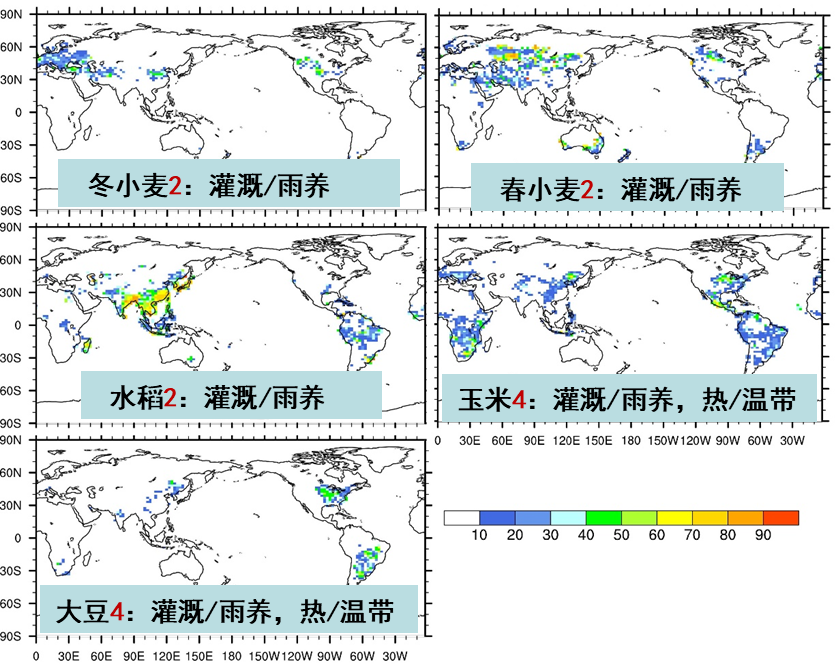
\includegraphics[scale=0.9]{Figures/作物模式/GPAM1模式模拟的14个作物功能类型格点面积覆盖率空间分布.png}
    \caption{GPAM1模式模拟的14个作物功能类型(CFT)格点面积覆盖率(\%)的空间分布}
    \label{fig:作物功能类型覆盖率的空间分布}
  \end{figure}
}

\section{物候}
GPAM1的物候包括三个阶段: (1)播种到抽芽; (2)抽芽到开始灌浆(grain fill); (3)灌浆到成熟/收割。所涉及的参数取值见表~\ref{tab:作物物候方案相关参数}。

% Please add the following required packages to your document preamble:
% \usepackage{booktabs}
\begin{table}[htbp]
  \centering
  \caption{作物物候方案相关参数}
  \label{tab:作物物候方案相关参数}
  \begin{tabular}{@{}cccccc@{}}
    \toprule
           & $T_{\mathrm{base}}$ & $f_{\mathrm{LE}}$ & $f_{\mathrm{GF}}$ & $GDD_{\mathrm{mat}}$  & $GSL_{\mathrm{max}}$ \\ \midrule
    春小麦 & 0                   & 0.07              & 0.60              & 0.2$GDD_{10yr}$+1458  & 150                  \\
    冬小麦 & 0                   & 0.03              & 0.67              & 0.38$GDD_{10yr}$+526  & 270                  \\
    水稻1  & 10                  & 0.12              & 0.68              & 0.30$GDD_{10yr}$+695  & 150                  \\
    水稻2  & 10                  & 0.35              & 0.75              & 0.27$GDD_{10yr}$+575  & 150                  \\
    玉米   & 8                   & 0.11              & 0.64              & 0.26$GDD_{10yr}$r+907 & 150                  \\
    大豆   & 10                  & 0.15              & 0.69              & 0.26$GDD_{10yr}$+802  & 150                  \\ \bottomrule
  \end{tabular}
\end{table}

\subsection{播种}\label{sec:播种}
  播种日期是给定的,采用全球播种日再分析数据~\citep{jagermeyr2021climate}),并结合陆表数据中的作物分布制作而成 (图~\ref{fig:GPAM1播种日空间分布}),为GPAM1的输入场。

{
\begin{figure}[htbp]
  \centering
  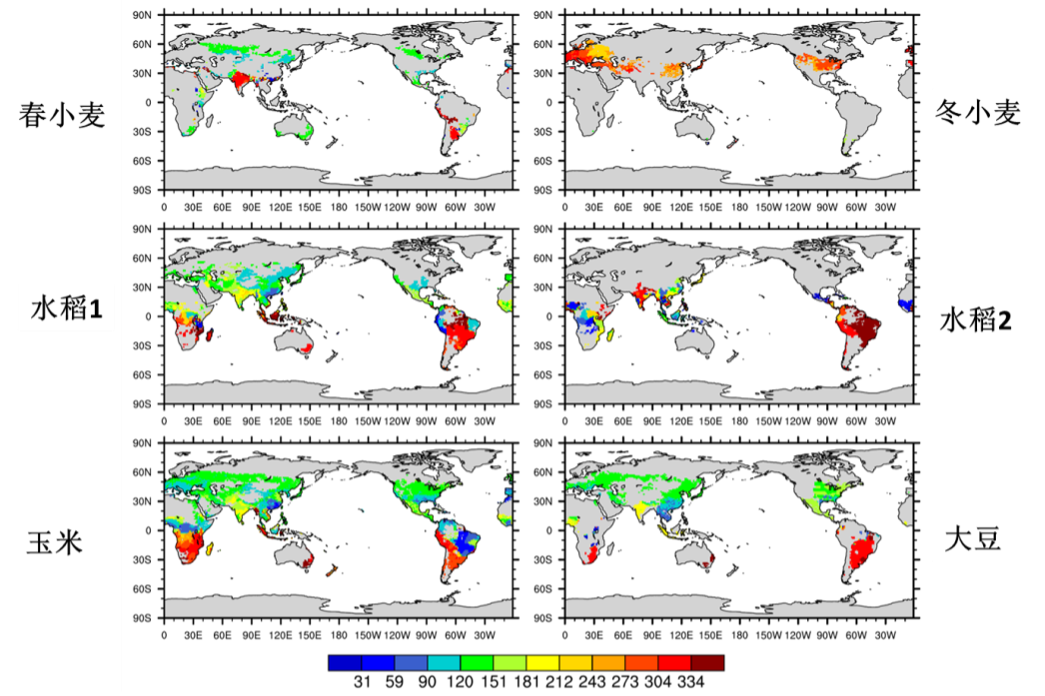
\includegraphics[scale=1.2]{Figures/作物模式/GPAM1播种日空间分布.png}
  \caption{GPAM1播种日空间分布}
  \label{fig:GPAM1播种日空间分布}
\end{figure}
}

\subsection{抽芽}
当热单元指数(Heat Unit Index, ${\mathrm {HUI}}$):
\begin{equation}\label{HUI}
  {\mathrm {HUI}}=\frac{GDD_{\mathrm{base}}}{GDD_{\mathrm{mat}}}
\end{equation}
达到$f_{\mathrm{LE}}$时,开始抽芽。$GDD_{\mathrm{base}}$是基于陆表气温的积温(\textcelsius\ days):
\begin{equation}
  GDD_{\mathrm{ {base }}}=\sum_{\mathrm{planting}}^{current\ day} \min \left(0, T_{\mathrm{sa}}-T_{\mathrm{base}}\right)
\end{equation}
其中,$T_{\mathrm{sa}}$是日地表气温,$T_{\mathrm{base}}$是底温(作物在该温度下停止生长)。

\subsection{灌浆}
当${\mathrm {HUI}}$达到$f_{\mathrm{GF}}$时,开始灌浆。

\subsection{成熟}
当${\mathrm {HUI}}$达到1时或生长季达到最长生长季长度$GSL_{\mathrm{max}}$时,作物成熟。其中,$GDD_{\mathrm{mat}}$是$GDD_{\mathrm{base}}$
10年滑动平均的一元线性方程(表~\ref{tab:作物物候方案相关参数})。
\begin{equation}
  GDD_{\mathrm{mat}}=a GDD_{10yr}+b
\end{equation}

\subsection{收割}
假设达到成熟的时步收割。


\section{生理变化}
作物的碳(C)库和氮(N)库有leaf, live stem, grain, fine root库及相应的transfer和storage库,无dead stem, live coarse root, dead coarse root库及相应的transfer和storage库。由于新加了grain库,相应通量会增加分配到grain的C/N通量,grain到Aproduct及litter的C/N通量。作物的呼吸和周转与草相同。

\subsection{光合和气孔导度}
大豆、小麦、水稻采用C3植物光合方案;玉米采用C4植物光合方案。
在基于Medlyn方案计算气孔导度时,玉米的参数取值$g_1=1.8$,低于自然植被,其余作物的参数取值$g_1=5.8$,高于自然植被。该参数越大,气孔导度越高。

\subsection{分配}
分配系数随物候阶段变化而变化。从出叶开始,按下列分配系数公式分配到叶库Cleaf,茎库Cleaf,根库Croot,粒库Cgrain。
不同物候期分配系数见表~\ref{tab:作物分配方案相关参数}。

(1)	物候期2 \\
\begin{equation}
  \left\{\begin{array}{c}
      a_{\mathrm{grain}}=0 \\
      a_{\mathrm{root}}=a_{\mathrm{root\_i}}-\left(a_{\mathrm{root\_i}}-a_{\mathrm{root\_f}}\right) {\mathrm {HUI}} \\
      a_{\mathrm{leaf}}=\left(1-a_{\mathrm{root}}\right) a_{\mathrm{leaf\_i}} \frac{{e}^{-{b}}-{e}^{-b \frac{{\mathrm {HUI}}}{f_{\mathrm{GF}}}}}{{e}^{-{b}}-1}   \\
      a_{\mathrm{stem}}=1-a_{\mathrm{grain}}-a_{\mathrm{root}}-a_{\mathrm{leaf}}
  \end{array}\right.
\end{equation}
其中,下标$i$和$f$表示该分配系数的初值和终值,$b=0.1$。

(2)	物候期3 \\
\begin{equation}
  \left\{\begin{array}{c}
      a_{\mathrm{leaf}}=0.0 \\
      a_{\mathrm{root}}=a_{\mathrm{root\_i}}-\left(a_{\mathrm{root\_i}}-a_{\mathrm{root\_f}}\right) \min(1, {\mathrm {HUI}}) \\
      a_{\mathrm{stem}}=\max \left[a_{\mathrm{stem\_f}}, a_{\mathrm{stem}} \max \left(0, \frac{1-{\mathrm {HUI}}}{1-f_{\mathrm{GF}}}\right)^{d_{\mathrm{sem}}}\right] \\
      a_{\mathrm{grain}}=1-a_{\mathrm{root}}-a_{\mathrm{leaf}}-a_{\mathrm{stem}}
  \end{array}\right.
\end{equation}
% Please add the following required packages to your document preamble:
% \usepackage{booktabs}
\begin{table}[htbp]
  \centering
  \caption{作物分配方案相关参数}
  \label{tab:作物分配方案相关参数}
  \begin{tabular}{@{}lcccc@{}}
    \toprule
    参数                        & 小麦 & 水稻 & 玉米 & 大豆 \\ \midrule
    $\alpha_{\mathrm{leaf\_i}}$ & 0.9  & 0.75 & 0.8  & 0.85 \\
    $\alpha_{\mathrm{root\_i}}$ & 0.1  & 0.1  & 0.4  & 0.2  \\
    $\alpha_{\mathrm{root\_f}}$ & 0    & 0    & 0.05 & 0.2  \\
    $\alpha_{\mathrm{stem\_f}}$ & 0.05 & 0.05 & 0.0  & 0.3  \\
    $d_{\mathrm{stem}}$         & 1    & 1    & 2    & 5    \\ \bottomrule
  \end{tabular}
\end{table}

\subsection{氮循环}
作物的氮循环和自然植被类似,但碳氮比(CN)不同。CoLM采用的作物不同组织的碳氮比CN如表~\ref{tab:作物碳氮比}所示。其中,碳氮比CNleaf, CNstem, CNroot用于灌浆前,其余碳氮比用于灌浆开始后。

此外,我们考虑了大豆根瘤中的根瘤菌与大豆共生固氮,大豆共生固氮能力设为自然植物的4倍,假设其余作物类型无生物共生固氮能力。生物共生固定的氮直接到 $\mathrm{NO_3^-}$ 库。

%(1) 碳氮比(CN)\\
%表~\ref{tab:作物碳氮比} 中,碳氮比$CN_{\mathrm{leaf}}$,$ CN_{\mathrm{stem}}$, %$CN_{\mathrm{root}}$用于灌浆前,其余碳氮比用于灌浆开始后。\\
% Please add the following required packages to your document preamble:
% \usepackage{booktabs}
\begin{table}[htbp]
  \centering
  \caption{作物碳氮比}
  \label{tab:作物碳氮比}
  \begin{tabular}{@{}lcccc@{}}
    \toprule
    参数                     & 小麦 & 水稻 & 玉米 & 大豆 \\ \midrule
    $CN_{\mathrm{leaf}}$     & 20   & 20   & 25   & 20   \\
    $CN_{\mathrm{stem}}$     & 50   & 50   & 50   & 50   \\
    $CN_{\mathrm{root}}$     & 42   & 42   & 42   & 42   \\
    $CN_{\mathrm{leaf\_f}}$  & 65   & 65   & 65   & 65   \\
    $CN_{\mathrm{stem\_f}}$  & 100  & 100  & 120  & 130  \\
    $CN_{\mathrm{root\_f}}$  & 40   & 40   & 0    & 0    \\
    $CN_{\mathrm{grain\_f}}$ & 50   & 50   & 50   & 50   \\ \bottomrule
  \end{tabular}
\end{table}

%(2) 大豆共生固氮 (SNF)\\
%考虑大豆根瘤中的根瘤菌与大豆共生固氮,大豆共生固氮能力设为自然植物的4倍,假设其余作物类型无生物共生固氮能力。生物共生固定的氮直接被植物吸收。\\
%

%\section{光合作用和气孔导度}
%大豆、小麦、水稻采用C3植物光合方案;玉米采用C4植物光合方案。
%在基于Medlyn方案计算气孔导度时,玉米的参数取值$g_1=1.8$,低于自然植被,其余作物的参数取值$g_1=5.8$,高于自然植被。该参数越大,气孔导度越高。
%


\subsection{冬小麦春化现象}
春化响应$V$(0$\sim$1)采用~\citet{streck2003incorporating}方案:
\begin{equation}
  V=\frac{D_{\mathrm{v}}{ }^{5}}{22.5^{5}+D_{\mathrm{v}}^{5}}
\end{equation}
其中,$D_{\mathrm {v}} $是物候阶段2累积的日春化率:
\begin{equation}\label{D_v_a}
  D_{\mathrm{v}}=\sum R_{\mathrm{v}}
\end{equation}
在公式(\ref{D_v_a})中,$R_{\mathrm{v}}$是日地表温度的函数:
\begin{equation}
  R_{\mathrm{v}} = \begin{cases}
    \frac{\left[2\left(T-T_{\mathrm{min}}\right)^{a}\left(T_{\mathrm{opt}}-T_{\mathrm{min}}\right)^{a} - \left(T-T_{\mathrm{min}}\right)^{2a}\right]}{\left(T_{\mathrm{opt}}-T_{\mathrm{min}}\right)^{2a}}, &T_{\mathrm{min}} \leqslant T \leqslant T_{\mathrm{max}} \\
    0,  &T<T_{\mathrm{min}} \quad  \text{or} \quad T>T_{\mathrm{max}}
  \end{cases}
\end{equation}
其中,$T_{\mathrm{min}}$= –1.3 \textcelsius, $T_{\mathrm{opt}}$= 4.9 \textcelsius, $T_{\mathrm{max}}$= 15.7 \textcelsius。$ R_{\mathrm {v}} $ 的取值从 0 (当$ T\leqslant T_{\mathrm{min}}$ 或者 $ \geqslant  T_{\mathrm{max}}$) 到 1 ( 当$T=T_{\mathrm{opt}}$)。
\begin{equation}
  a=\frac{\ln 2}{\ln \left[\left(T_{\max }-T_{\min }\right) /\left(T_{\mathrm{o p t}}-T_{\min }\right)\right]}
\end{equation}

春化响应用于调整$GDD_{\mathrm{base}}$和粒分配系数
\begin{equation}
  G D D_{\mathrm{b a s e}}=G D D_{\mathrm{b a s e,  { unadjusted }}} \times V
\end{equation}
\begin{equation}
  a_{\mathrm{ {grain }}}=a_{\mathrm{ {grain,unadjusted }}} \times V_{\mathrm{f}}
\end{equation}


\section{胁迫}
\subsection{臭氧污染胁迫}
%\section{臭氧污染胁迫}
考虑臭氧对光合速率和气孔导度的影响因子 $F_{\mathrm{O3\_A}}$ 以及$F_{\mathrm{O3\_{gs}}}$:
\begin{equation}
  F_{\mathrm{O3\_{A}}}=-0.0022 POD_{\mathrm{0.5}}+0.868
\end{equation}
\begin{equation}
  F_{\mathrm{O3\_{gs}}}=-0.00096 POD_{\mathrm{0.5}}+0.856
\end{equation}
其中,$POD_{0.5}$ (Phytotoxic ozone dose above a threshold of 0.5 \unit{nmol.m^{-2}.s^{-1}}, 单位:\unit{mmol.m^{-2}})是植物吸收的$O_3$通量在抽芽后生长季白天的累积量。第 $t$ 时间步的 $\mathrm{O_3}$ 通量累积量:
\begin{equation}\label{eq:POD05}
  POD_{0.5,t}=POD_{0.5,t-1}\left(1-D_t\right)+U_{0.5,t} \times 10^{-6}.
\end{equation}
在公式\eqref{eq:POD05}中,$D_t$是$t$时步的$\mathrm{O_3}$通量累积量衰减率:
\begin{equation}
  D_t = \max\left(0, 1-\frac{LAI_{t-1}}{LAI_t} \right),
\end{equation}
$t$ 时步的$\mathrm{O_3}$通量累积量:
\begin{equation}
  U_{\mathrm{Y,t}}=\begin{cases}
    \Delta t\times\max(F_{{\mathrm {O3}},t}-Y, 0) & \text{白天} \\
    0 & \text{其它时间}
  \end{cases},
\end{equation}
其中 $\Delta t$ 是时间步长 (s); 而 $t$ 时步的$\mathrm{O_3}$通量:
\begin{equation}
  F_{{\mathrm {O3}},t}=\frac{\mathrm{[O_3]}}{r_{\mathrm {b}}  + r_{\mathrm{am}} + r_{\mathrm s}k_{\rm O3}},
\end{equation}
其中$\mathrm{[O_3]}$ 为陆面参考高度大气的臭氧浓度(\unit{nmol.m^{-3}}), $r_{\rm am}$ (\unit{s.m^{-1}})、$r_{\mathrm {b}} $ (\unit{s.m^{-1}}) 和 $r_{\mathrm {s}} $ (\unit{s.m^{-1}}) 分别为空气动力学阻抗、大气边界层阻抗、叶气孔阻抗,$k_{\rm O3}=0.663$ 为臭氧和水蒸气的扩散比。

上面计算的$F_{\mathrm{{O3}\_A}}$ 以及$F_{\mathrm{O3\_{gs}}}$分别作用在Farquhar--Collatz方案计算的光合速率以及Ball--Berry方案计算出的气孔导度。

\subsection{热胁迫}
作物对热胁迫的敏感期大约是在开花前后及灌浆期,在GPAM1里设为${\mathrm {HUI}} $满足$0.5 \leqslant {\mathrm {HUI}} \leqslant 0.8$的时段。在每个发生热胁迫的时步,采用场数损失率$l$:
\begin{equation}
  l=\left\{\begin{array}{cc}1-\left(\frac{4.3}{10.4}\right)^{\frac{\Delta t}{3600\times 21}} & T>T_{\mathrm{c}} \\ 0 & T \leqslant T_{\mathrm{c}}\end{array}\right.
\end{equation}
其中,$\Delta t$ 是时步长,$T$是该时步的温度;$T_{\mathrm {c}} $是临界温度:$T_{\mathrm {c}} =34$ \textcelsius (水稻,玉米,冬小麦),31 \textcelsius (春小麦),37 \textcelsius (大豆)。
每个时步考虑了热胁迫后的叶$C_{\mathrm{leaf}}$库为:
\begin{equation}
  C_{\mathrm{leaf}}=C_{\mathrm{leaf,  {unadjusted}}} \times (1-l)
\end{equation}


\section{管理}
\subsection{施肥}
氮肥考虑了工业氮肥和粪肥。工业氮肥是输入场。粪肥设为2 \unit{g.N.m^{−2}.yr^{−1}}。施肥时直接将氮肥输入土壤 $\mathrm{NH_4^+}$ 库,从出叶开始,以匀速的方式施肥 20 天。

\subsection{收割和农业残留物处理}
收割时粒库 $\mathrm{C_{\mathrm{grain}}}$ 进入种子库 $\mathrm{C_{\mathrm{seed}}}$ 和食品库 $\mathrm{C_{\mathrm{food}}}$
\begin{equation}
  \mathrm{{C}_{\mathrm{seed}}}=\min \left(\mathrm{C_{\mathrm{grain}}}, 3\right)
\end{equation}
\begin{equation}
  \mathrm{C_{\mathrm{food}}}=\mathrm{C_{\mathrm{grain}}}-\mathrm{C_{\mathrm{seed}}}
\end{equation}
其中,种子库$\mathrm{C_{\mathrm{seed}}}$在下一个生长季出叶期的第一时步转移到叶库$\mathrm{C_{\mathrm{leaf}}}$。叶和茎的碳库进入地上凋落物库。根的碳库进入地下凋落物库。

\subsection{秸秆焚烧及排放}
秸秆焚烧燃烧面积百分率${\mathrm {BAF}}$(\unit{s^{-1}}):
\begin{equation}
  BAF= a_1 f_{\mathrm{se}} f_{\mathrm{crop}}
\end{equation}
其中,$a_1$ (\unit{s^{-1}})是全球常数;$f_{\mathrm{se}}$ 是社会经济因子的影响:
\begin{equation}
  f_{\mathrm{se}} = f_{\mathrm {d}}  f_{\mathrm {e}}
\end{equation}
其中,
\begin{equation}
  f_{\mathrm {d}}  = 0.04 + 0.96\exp\left[-\pi\left(\frac{D_{\mathrm {p}} }{350}\right)\right]
\end{equation}
\begin{equation}
  f_{\mathrm {e}}  = 0.01 + 0.99\exp\left[-\pi\frac{GDP}{10}\right]
\end{equation}
$D_{\mathrm {p}} $ (\unit{person.km^{-2}}) 及 ${\mathrm {GDP}}$ (\unit{k\ 1995\ US\$.capita^{-1}})
分别是人口密度和生产总值。
$f_{\mathrm{crop}}$ 用于判断火发生时间(发生时为1,其余时步为0),
是输入场,定义为观测播前观测的秸秆焚烧峰值时步。
观测的秸秆焚烧峰值时步基于GFED4s的3小时数据;播种时间见章节~\ref{sec:播种}。

在得到燃烧面积后,火灾引起的碳排放${\mathrm {CE}}$ (\unit{g.C.m^{-2}.s^{-1}}) 为:
\begin{equation}
  CE=BAF \times C_{\mathrm{ab,litter}} \times CC
\end{equation}
$C_{\mathrm{ab,litter}}$是地上凋落物碳库, $CC=0.8$是燃烧完全因子。

此后,我们估算火灾引起的33种痕量气体和气溶胶排放。火灾引起的第$i$类痕量气体和气溶胶排放量$E_i$ (\unit{g.species.m^{-2}.s^{-1}}):
\begin{equation}
  E_{i}=EF_{i} \times CE /[{C}]
\end{equation}
$EF_i$ (\unit{g.species.(kg.dry\ matter(DM))^{-1}})是排放因子,见表~\ref{tab:秸秆焚烧排放因子取值}。$[C]=$ \qty{0.5e3}{g.C.(kg.DM)^{-1}}是单位转换因子。


% Please add the following required packages to your document preamble:
% \usepackage{booktabs}
\begin{table}[htbp]
  \centering
  \caption{秸秆焚烧排放因子取值(\unit{g.species.(kg.DM)^{-1}})}
  \label{tab:秸秆焚烧排放因子取值}
  \begin{tabular}{@{}lc|lc@{}}
    \toprule
    种类               & 排放因子 & 种类                   & 排放因子 \\ \midrule
    CO2                & 1421     & C2H4   (ethylene)      & 1.14     \\
    CO                 & 78       & C3H6   (propylene)     & 0.48     \\
    CH4                & 5.9      & C5H8   (isoprene)      & 0.18     \\
    NMHC               & 5.8      & C10H16   (terpenes)    & 0.03     \\
    H2                 & 2.65     & C7H8   (toluene)       & 0.18     \\
    NOx                & 2.67     & C6H6   (benzene)       & 0.31     \\
    N2O                & 0.09     & C8H10   (xylene)       & 0.09     \\
    PM2.5              & 8.5      & CH2O   (formaldehyde)  & 1.80     \\
    TPM                & 11.3     & C2H4O   (acetaldehyde) & 1.82     \\
    TPC                & 5.5      & C3H6O   (acetone)      & 0.61     \\
    OC                 & 5.0      & C3H6O2(hydroxyacetone) & 1.74     \\
    BC                 & 0.43     & C6H5OH   (Phenol)      & 0.50     \\
    SO2                & 0.81     & NH3 (ammonia)          & 1.04     \\
    C2H6   (ethane)    & 0.76     & HCN (hydrogen cyanide) & 0.43     \\
    CH3OH   (methanol) & 2.63     & MEK/2-butanone         & 0.60     \\
    C3H8   (propane)   & 0.20     & CH3CN   (acetonitrile) & 0.25     \\
    C2H2   (acetylene) & 0.32     &                        &          \\ \bottomrule
  \end{tabular}
\end{table}


\subsection{灌溉}
CoLM灌溉方案基于\citet{ozdogan2010simulating} 和 \citet{yao2022Irrigation}方案,在灌溉作物种类的播种区考虑。

CoLM灌溉模块主要分为三部分:计算潜在灌溉需求水量;计算灌溉供应水量;计算灌溉施加水通量,实现对灌溉过程的模拟。考虑到实际灌溉方式在全球存在显著差异,因此每种作物在不同网格分别采用了滴灌、喷灌、漫灌、稻田灌溉四种不同的灌溉方式。

当地时间每天早上6点,模块将判断是否有正在生长的灌溉作物,如果存在,则将逐步计算灌溉需求量、灌溉供应量以及灌溉施加。

首先,计算潜在灌溉需求水量(mm):
\begin{equation}
  D_{\mathrm{irrig}} = \begin{cases}
    \omega_{\mathrm{irrig}} - \omega_{\mathrm{avail}} & \omega_{\mathrm{thresh}} > \omega_{\mathrm{avail}} \\
    0     & \omega_{\mathrm{thresh}} \leqslant \omega_{\mathrm{avail}}
  \end{cases},
\end{equation}
其中,$\omega_{\mathrm{avail}}$ 为土壤当前总水量(mm):
\begin{equation}\label{eq:omega-avail}
  \omega_{\mathrm{avail}} = \sum_{\mathrm{j=1}}^{N_{\mathrm{irr}}}\theta_j\Delta z_j;
\end{equation}
$\omega_{\mathrm{irrig}}$ 为实际灌溉目标水量(mm):
\begin{equation}
  \omega_{\mathrm{irrig}} = f_{\mathrm{thresh}}(\omega_{\mathrm{target}}-\omega_{\mathrm{wilt}}) + \omega_{\mathrm{wilt}},
\end{equation}
其中,$\omega_{\mathrm{target}}$ 为灌溉目标水量(mm):
\begin{equation}
  \omega_{\mathrm{target}} = \sum_{\mathrm{j=1}}^{N_{\mathrm{irr}}}\theta_{\mathrm{target}}\Delta z_j,
\end{equation}
$\omega_{\mathrm{wilt}}$ 为萎蔫点土壤水量(mm):
\begin{equation}\label{eq:omega-wilt}
  \omega_{\mathrm{wilt}} = \sum_{\mathrm{j=1}}^{N_{\mathrm{irr}}}\theta_{\mathrm{wilt}}\Delta z_j.
\end{equation}
方程\eqref{eq:omega-avail}--\eqref{eq:omega-wilt}中,$N_{\mathrm{irr}}$ 为发生灌溉土壤层数,与设定灌溉深度$z_{\mathrm{irrig}}$有关;$\Delta z_j$ 为第$j$层土壤厚度;$\theta_{\mathrm{target}}$、$\theta_{\mathrm{wilt}}$和$\theta_j$ 则分别为土壤各层的灌溉目标湿度、田间萎蔫点以及土壤实际湿度,需要根据其对应的土壤水势$\Phi_{\mathrm{target}}$、 $\Phi_{\mathrm{wilt}}$和$\Phi_j$ 计算。

由于不同灌溉方式的触发灌溉阈值和目标灌溉量存在差异,灌溉触发阈值为:
\begin{equation}
  \omega_{\mathrm{thresh}} = f_{\mathrm{thresh}}(\omega_{\mathrm{trigger}}-\omega_{\mathrm{wilt}}) + \omega_{\mathrm{wilt}},
\end{equation}
其中 $\omega_{\mathrm{trigger}}$ 为触发灌溉的目标水量,根据 $\Phi_{\mathrm{trigger}}$ 计算,$f_{\mathrm{thresh}}$ 为灌溉调优参数,$\omega_{\mathrm{thresh}}$ 为触发灌溉水量阈值。相应的灌溉方案参数见表~\ref{tab:灌溉方案参数}。

\begin{table}[htbp]
  \centering
  \caption{灌溉方案参数}
  \label{tab:灌溉方案参数}
  \begin{threeparttable}
    \begin{tabular}{@{}ccccc}
      \toprule
                                    & drip    & sprankler & flood                 & paddy                 \\ \midrule
      $f_{\mathrm{thresh}}$         & 1       & 1         & 1                     & 1                     \\
      $z_{\mathrm{irrig}}(m)$       & 0.6     & 0.6       & 0.6                   & 0.6                   \\
      $\Phi_{\mathrm{target}}$(mm)  & -3300   & -3300     & $\Phi_{\mathrm{sat}}$ & $\Phi_{\mathrm{sat}}$ \\
      $\Phi_{\mathrm{trigger}}$(mm) & -3300   & -3300     & -3300                 & $\Phi_{\mathrm{sat}}$ \\
      $\Phi_{\mathrm{wilt}}$ (mm)   & -150000 & -150000   & -150000               & -150000               \\ \bottomrule
    \end{tabular}
    \begin{tablenotes}
      \footnotesize
    \item[注:] $\Phi_{\mathrm{sat}}$ 为饱和水势。
    \end{tablenotes}
  \end{threeparttable}
\end{table}

计算灌溉供应水量,假设灌溉需求灌溉量可全部被地下水提供。

计算灌溉施加水通量时,考虑到实际灌溉策略,假定灌溉发生后,实际灌溉水量将在4小时内,根据灌溉方式均匀施加。其中喷灌施加在作物冠层,经历冠层截留到达地表;而其他灌溉方式则直接将水施加在地表。

灌溉速率$R_{\mathrm{irrig}}$ 为:
\begin{equation}
  R_{\mathrm{irrig}} = \frac{D_{\mathrm{irrig}}}{T_{\mathrm{irrig}}},
\end{equation}
其中,$T_{\mathrm{irrig}}$ 为灌溉持续时间(默认值14400 s)。
\section{结构形态}
出叶后到收割前,叶面积为:
\begin{equation}
  {\rm LAI}=C_{\mathrm{leaf}} \times SLA
\end{equation}
SLA为比叶面积 (\unit{m^2.leaf.g^{-1}.C})(表~\ref{tab:结构形态参数})。

茎叶面积为:
\begin{equation}
  {\rm SAI}=\left\{\begin{array}{lcc}0.1 {\rm LAI}, & \text { for } & \text { maize } \\
  0.2 {\rm LAI}, & \text { for } & \text {others}\end{array}\right.
\end{equation}

冠层顶高度$z_{\mathrm{top}}$(米)和冠层底高度$z_{\mathrm{bot}}$(米)为:
\begin{equation}
  z_{\mathrm{top}}=\max \left[0.05, z_{\mathrm{top,max}} \min \left(\frac{{\mathrm {HUI}}}{f_{\mathrm{GF}}}, 1.0\right)\right]
\end{equation}
\begin{equation}
  z_{\mathrm{b o t}}=0.02
\end{equation}

% Please add the following required packages to your document preamble:
% \usepackage{booktabs}
\begin{table}[htbp]
  \centering
  \caption{结构形态参数}
  \label{tab:结构形态参数}
  \begin{tabular}{@{}lccccc}
    \toprule
    参数                   & 春小麦 & 冬小麦 & 水稻   & 玉米   & 大豆   \\ \midrule
    ${\mathrm {SLA}}$      & 0.0453 & 0.0441 & 0.0431 & 0.0409 & 0.0566 \\
    $z_{\mathrm{top,max}}$ & 0.808  & 0.852  & 0.98   & 2.55   & 0.823  \\ \bottomrule
  \end{tabular}
\end{table}

\chapter{湖泊模式}\label{ch:湖泊模式}
%\addcontentsline{toc}{chapter}{湖泊模式}
\begin{mymdframed}{代码}
  本章对应的代码文件为\texttt{MOD\_Lake.F90}。
\end{mymdframed}

湖泊作为陆地表面一种特定形式的水体,对区域尺度的水热平衡过程及气候变化具有显著影响,其中大面积的湖泊对于局地的天气和气候可起到决定性作用。
为模拟湖泊的热力和动力过程,湖泊模式在上世纪80年代开始发展~\citep{henderson1985new},
并逐渐形成针对不同湖泊的简易湖泊模式~\citep{hostetler1993interactive,hostetler1994lake,hostetler1990simulation}。
此后,湖泊模式作为陆面过程模式的重要组成模块,其应用逐渐发展到针对全球湖泊的普适性模拟(e.g. \citet{bonan1995sensitivity,bonan1996land})。
\citet{zeng2002coupling}对当时已有的湖泊模式进行了改进,
使得湖泊模式的模拟效果得到显著提高,成为通用陆面模式CoLM中湖泊模型的早期版本(CoLM-Lake)。
近几年来,随着湖泊模型的不断发展,CoLM-Lake逐渐纳入了新的针对湖泊方案的发展与改进,
并在2014年发布的新版CoLM中对湖泊模型进行了更新。本章将对新版CoLM-Lake的物理方案做一详细描述(图~\ref{fig:湖泊系统垂直分层示意图})。

{
  \begin{figure}[htbp]
    \centering
    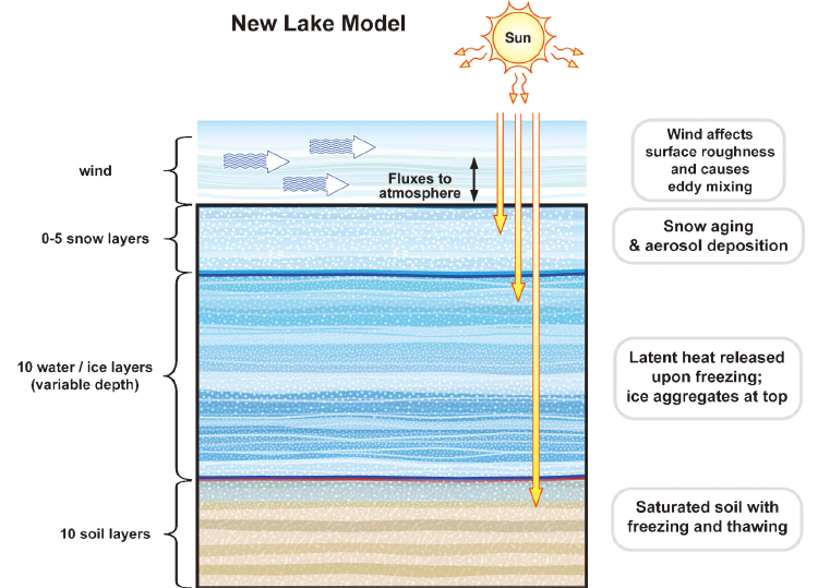
\includegraphics{Figures/湖泊模式/湖泊系统垂直分层示意图.png}
    \caption{湖泊系统垂直分层示意图 \citep{subin2012improved}}
    \label{fig:湖泊系统垂直分层示意图}
  \end{figure}
}


\section{湖泊模式结构}
湖泊模式由三部分组成:雪层、湖泊层和淤泥层。湖泊层位于雪层和淤泥层之间,
共分为10层。湖泊深度可随降水量、蒸发量、与湖泊连接的河流的流入流出量等发生变化(见~\ref{湖泊水文}~节)。在初始时刻,默认湖深$d$为50 m,每层湖泊的厚度$\Delta z_{\mathrm{lake},i}$从上到下分别为0.1, 1, 2, 3, 4, 5, 7, 7, 10.45, 10.45 m,
中心深度$z_{\mathrm{lake},i}$为每层湖泊的中间位置所在深度,分别为0.05, 0.6, 2.1, 4.6, 8.1, 12.6, 18.6, 25.6, 34.325, 44.775 m。
湖泊深度$d$亦可由地表参数数据集提供。当$d\neq50$ m且$d\geqslant 1$ m时,第一层湖泊的厚度仍保持0.1 m,
其余层厚度按照上述分层厚度的比例进行分配。
当$d<1$ m时,10层湖泊进行等分。在模式中,每层湖泊的质量固定不变,由液态水密度与每层湖泊的厚度确定,
湖泊状态变量由混合层深度、湖冰厚度和每一层湖泊的温度$T_{\mathrm{lake}}$与冻结部分所占的质量比$I$来表征。雪层与淤泥层的分层方式与~\ref{温度求解的数值格式} 节介绍的计算雪盖淤泥温度时的分层方案相同
,物理方案遵从无植被覆盖下的土壤雪盖状态变量的计算方案来设定。


\section{降水与湖泊表面的相互作用}
降水到达湖泊表面可发生能量转移与相态变化等一系列过程。此过程可改变湖泊表面条件,尤其当降雪存在时,对于湖泊之上雪层的形成起到决定性作用。


首先,在进行湖泊过程计算之前,对湖泊表面的积雪厚度$z_{\mathrm{sno}}$ (m)与雪水当量$W_{\mathrm{sno}}$ (mm或 \unit{kg.m^{-2}})进行更新:
\begin{equation}
  Z_{\mathrm{sno}}=Z_{\mathrm{sno}}+\frac{p_{\mathrm {snow}} \Delta t}{\rho_{\mathrm{sno,new}}}
\end{equation}
\begin{equation}
  W_{\mathrm{sno}}=W_{\mathrm{sno}}+p_{\mathrm {snow}} \Delta t
\end{equation}
其中$p_{\mathrm {snow}} $表示固态降水率(\unit{kg.m^{-2}.s^{-1}}),$\rho_{\mathrm{sno,new}}$表示新降的干雪密度(\unit{kg.m^{-3}})(见章节~\ref{温度求解的数值格式})。

接下来,计算湖泊表面与降水的能量转移过程,并且当降水与湖泊表面的相态不同时,相态变化过程同时考虑。
此过程将根据更新后的积雪厚度,分为湖泊表层
\begin{enumerate}
  \item 未达到第一层雪的产生条件;
  \item 已达到第一层雪产生条件但之前无雪层;
  \item 之前已存在雪层,三种情况进行计算。
\end{enumerate}

\noindent\textbf {(1)未达到第一层雪产生条件(即$z_{\mathrm{sno}}<0.01$且$snl=0$)}

此情形下,降水视为与第一层湖泊表面充分接触并立即发生能量转移,并且当降水与湖泊表层的相态不同时,相态变化过程同时发生。
此过程的演变由以下八个能量组份(\unit{J.m^{-2}})决定:
\begin{align*}
  a &= C_{\mathrm{liq}} p_{\mathrm {rain}} \Delta t\left(T_{\mathrm{p}}-T_{\mathrm {frz}}\right)   & \text{液态降水冷却到$T_{\mathrm {frz}} $释放的能量} \\
  b &= \lambda_{\mathrm {fus}}  p_{\mathrm {rain}}  \Delta t                                           & \text{液态降水凝结为固态释放的能量} \\
  c &= C_{\mathrm{ice}} \rho_{\mathrm{liq}} \Delta z_{\mathrm{lake, 1}} I_{1}\left(T_{\mathrm {frz}} -T_{\mathrm{lake, 1}}\right)  & \text{第一层湖泊固态下加热到$T_{\mathrm {frz}} $吸收的能量} \\
  d &= \lambda_{\mathrm {fus}}  \rho_{\mathrm{liq}} \Delta z_{\mathrm{lake, 1}} I_{1}         & \text{第一层湖泊固态下完全融化吸收的能量} \\
  e &= C_{\mathrm{ice}} p_{\mathrm {snow}}  \Delta t\left(T_{\mathrm {frz}}  -T_{\mathrm {p}} \right)        & \text{固态降水加热到$T_{\mathrm {frz}} $吸收的能量} \\
  f &= \lambda_{\mathrm {fus}}  p_{\mathrm {snow}}  \Delta t                                           & \text{固态降水融化为液态吸收的能量} \\
  g &= C_{\mathrm{liq}} \rho_{\mathrm{liq}} \Delta z_{\mathrm{lake, 1}}\left(1-I_{1}\right)\left(T_{\mathrm{lake, 1}}-T_{\mathrm {frz}} \right)  & \text{第一层湖泊液态下冷却到$T_{\mathrm {frz}} $释放的能量} \\
  h &= \lambda_{\mathrm {fus}}  \rho_{\mathrm{liq}} \Delta z_{\mathrm{lake, 1}}\left(1-I_{1}\right)  & \text{第一层湖泊液态下完全冻结释放的能量}
\end{align*}
其中,$p_{\mathrm {rain}} $、$p_{\mathrm {snow}} $分别为液态与固态降水率(\unit{kg.m^{-2}.s^{-1}}),$C_{\mathrm{liq}}$、$C_{\mathrm{ice}}$分别为液态水与固态水的比热容(\unit{J.kg^{-1}.K^{-1}}),
$T_{\mathrm {p}} $、$T_{\mathrm {frz}} $分别为雨水温度与液态水凝结温度(K),$\Delta t$表示时间积分步长(s),$\lambda_{\mathrm {fus}} $表示液态水凝结潜热(\unit{J.kg^{-1}}),
$\rho_{\mathrm{liq}}$表示液态水密度(\unit{kg.m^{-3}}),$T_{\mathrm{lake,1}}$,$\Delta z_{\mathrm{lake,1}}$,$I_1$分别为第一层湖泊的温度,
厚度与冻结部分所占的质量比。为表述清晰,此过程将按照第一层湖泊的不同相态分别考虑,计算如下:

A. 第一层湖泊完全冻结($I_1>0.999$)

此时,应有$T_{\mathrm{lake,1}}<T_{\mathrm {frz}} $。若固态降水发生($T_{\mathrm {p}} <T_{\mathrm {frz}} $),它将直接与湖泊表层达到一个平衡温度;
若液态降水发生($T_{\mathrm {p}} >T_{\mathrm {frz}} $),相态变化过程将会同时触发,具体如下:

若表层湖泊不需发生相态变化足以使得液态降水到达表面后凝结为固态,即$a\leqslant c-b$,则湖泊吸收的总能量为:
\begin{equation}
  C_{\mathrm{ice}} \rho_{\mathrm{liq}} \Delta z_{\mathrm{lake,1}} I_{1}\left(T_{\mathrm{lake, 1}}^{(n+1)}-T_{\text {lake,1 }}^{(n)}\right)=a+b+C_{\mathrm{ice}} p_{\mathrm {rain}} \Delta t\left(T_{\mathrm {frz}}-T_{\text {lake, }}^{(n+1)}\right)
\end{equation}
解出$T_{\mathrm{lake,1}}^{\left(n+1\right)}$即为此时更新的第一层湖泊温度。
同时后续计算中,液态降水可视为固态降水,雪水当量与积雪厚度随之更新:
\begin{equation}
  \begin{aligned}
    W_{\mathrm{sno}} &= W_{\mathrm{sno}}+p_{\mathrm {rain}}  \Delta t \\
    z_{\mathrm{sno}} &= z_{\mathrm{sno}}+\frac{p_{\mathrm {rain}}  \Delta t}{\rho_{\mathrm{sno,new}}} \\
    p_{\mathrm {snow}}  &= p_{\mathrm {snow}}  + p_{\mathrm {rain}}  \\
    p_{\mathrm {rain}}  &= 0.0
  \end{aligned}
\end{equation}


若表层湖泊将液态降水冷却到$T_{\mathrm {frz}} $后不足以冻结所有降水,即$c-b<a\leqslant c$,
则第一层湖泊温度更新为$T_{\mathrm{lake,1}}=T_{\mathrm {frz}} $。于是湖泊吸收的来自降水凝结的有效能量为$c-a$,
液态降水转为固态降水的量以及雪水当量和积雪厚度可更新为:
\begin{equation}
  \begin{aligned}
    W_{\mathrm{sno}} &= W_{\mathrm{sno}} + (c-a) / \lambda_{\mathrm {fus}}  \\
    z_{\mathrm{sno}} &= z_{\mathrm{sno}} + \frac{c-a}{\lambda_{\mathrm {fus}}  \rho_{\mathrm{sno,new}}} \\
    p_{\mathrm {snow}}  &= p_{\mathrm {snow}}  + \frac{c-a}{\lambda_{\mathrm {fus}}  \Delta t} \\
    p_{\mathrm {rain}}  &= p_{\mathrm {rain}}  - \frac{c-a}{\lambda_{\mathrm {fus}}  \Delta t}
  \end{aligned}
\end{equation}
若表层湖泊需要部分融化才可将液态降水冷却到$T_{\mathrm {frz}} $而降水无需发生相态变化,即$c<a\leqslant c+d$,
则第一层湖泊温度仍更新为$T_{\mathrm{lake,1}}=T_{\mathrm {frz}} $。于是降水冷却用于融化湖泊的有效能量为$a-c$,
此时湖泊冻结部分所占的质量比更新为:
\begin{equation}
  I_{1}=\frac{\rho_{\mathrm{liq}} \Delta z_{\mathrm{lake, 1}}-(a-c) / \lambda_{\mathrm {fus}}}{\rho_{\mathrm{liq}} \Delta z_{\mathrm{lake, 1}}}
\end{equation}
若表层湖泊可被液态降水完全融化而降水无需发生相态变化,即$a>c+d$,则降水释放的总能量为:
\begin{equation}
  C_{\mathrm{liq}} p_{\mathrm {rain}} \Delta t\left(T_{\mathrm{p}}-T_{\mathrm{lake, 1}}^{(n+1)}\right)=c+d+C_{\mathrm{liq}} \rho_{\mathrm{liq}} \Delta z_{\mathrm{lake, 1}}\left(T_{\mathrm{lake, 1}}^{(n+1)}-T_{\mathrm {frz}}\right)
\end{equation}
解出$T_{\mathrm{lake,1}}^{\left(n+1\right)}$即为此时更新的第一层湖泊温度,同时湖泊冻结部分质量比更新为$I_1=0.0$。


注意,经过以上情况讨论后,若发生液态降水冻结为固态降水,则雪水当量与积雪厚度将会增加。
此时若$z_{\mathrm{sno}}\geqslant 0.01$m,则第一层雪立即生成,且相应的状态变量设置为:
\begin{equation}
  \begin{aligned}
    snl &= -1 \\
    \Delta z_{0} &= z_{\mathrm{sno}} \\
    z_{0} &= -0.5 z_{\mathrm{sno}} \\
    z_{\mathrm{h,-1}} &= -\Delta z_{0} \\
    T_{0} &= T_{\mathrm{lake, 1}} \\
    w_{\mathrm{ice, 0}} &= W_{\mathrm{sno}} \\
    w_{\mathrm{liq, 0}} &= 0
  \end{aligned}
\end{equation}

B. 第一层湖泊为冰水混合态($0.001\leqslant I_1\leqslant 0.999$)

此时,应有$T_{\mathrm{lake,1}}=T_{\mathrm {frz}} $。若液态降水发生($T_{\mathrm {p}} >T_{\mathrm {frz}} $),
当液态降水可以将第一层湖泊中的冰全部融化时($a\geqslant d$),第一层湖泊的状态变量更新为:
\begin{equation}
  T_{\mathrm{lake, 1}}=\frac{C_{\mathrm{liq}} p_{\mathrm {rain}} \Delta t T_{\mathrm{p}}+C_{\mathrm{liq}} \rho_{\mathrm{liq}} \Delta z_{\mathrm{lake, 1}} T_{\mathrm {frz}}-d}{C_{\mathrm{liq}} \rho_{\mathrm{liq}} \Delta z_{\mathrm{lake, 1}}+C_{\mathrm{liq}} p_{\mathrm {rain}} \Delta t}
\end{equation}
\begin{equation}
  I_{1}=0.0
\end{equation}
否则,保持$T_{\mathrm{lake,1}}=T_{\mathrm {frz}} $,用于湖泊中冰融化的能量为$a$,则湖泊冻结部分的质量比更新为:
\begin{equation}
  I_{1}^{(n+1)}=\frac{\rho_{\mathrm{liq}} \Delta z_{\mathrm{lake, 1}} I_{1}^{(n)}-a / \lambda_{\mathrm {fus}}}{\rho_{\mathrm{liq}} \Delta z_{\mathrm{lake, 1}}}
\end{equation}
同样地,若固态降水发生($T_{\mathrm {p}} <T_{\mathrm {frz}} $),当固态降水可以将第一层湖泊中的水全部冻结时($e\geqslant h$),第一层湖泊的状态变量更新为:
\begin{equation}
  T_{\mathrm{lake, 1}}=\frac{C_{\mathrm{ice}} p_{\mathrm {snow}} \Delta t T_{\mathrm{p}}+C_{\mathrm{ice}} \rho_{\mathrm{liq}} \Delta z_{\mathrm{lake, 1}} T_{\mathrm {frz}}+h}{C_{\mathrm{ice}} \rho_{\mathrm{liq}} \Delta z_{\mathrm{lake, 1}}+C_{\mathrm{ice}} p_{\mathrm {snow}} \Delta t}
\end{equation}
\begin{equation}
  I_{1}=1.0
\end{equation}
否则,保持$T_{\mathrm{lake,1}}=T_{\mathrm {frz}} $,用于湖泊中水冻结的能量为$e$,则湖泊冻结部分的质量比更新为:
\begin{equation}
  I_{1}^{(n+1)}=\frac{\rho_{\mathrm{liq}} \Delta z_{\mathrm{lake, 1}} I_{1}^{(n)}+e / \lambda_{\mathrm {fus}}}{\rho_{\mathrm{liq}} \Delta z_{\mathrm{lake, 1}}}
\end{equation}

C. 	第一层湖泊完全融化($I_1<0.001$)

此时,应有$T_{\mathrm{lake,1}}>T_{\mathrm {frz}} $。若液态降水发生($T_{\mathrm {p}} >T_{\mathrm {frz}} $),它将直接与湖泊表层达到一个平衡温度;
若固态降水发生($T_{\mathrm {p}} <T_{\mathrm {frz}} $),相态变化过程将会同时触发,具体如下:

若表层湖泊不需发生相态变化足以使得固态降水到达表面后融化为液态,即$e\leqslant g-f$,则湖泊释放的总能量为:
\begin{equation}
  C_{\mathrm{liq}} \rho_{\mathrm{liq}} \Delta z_{\mathrm{lake, 1}}\left(1-I_{1}\right)\left(T_{\mathrm{lake, 1}}^{(n)}-T_{\mathrm{lake, 1}}^{(n+1)}\right)=
  e+f+C_{\mathrm{liq}} p_{\mathrm {snow}} \Delta t\left(T_{\mathrm{lake, 1}}^{(n+1)}-T_{\mathrm {frz}}\right)
\end{equation}
解出$T_{\mathrm{lake,1}}^{\left(n+1\right)}$即为此时更新的第一层湖泊温度。
同时后续计算中,固态降水可视为液态降水,雪水当量与积雪厚度随之更新:
\begin{equation}
  \begin{aligned}
    W_{\mathrm{sno}} &= W_{\mathrm{sno}}-p_{\mathrm {snow}} \Delta t \\
    z_{\mathrm{sno}} &= z_{\mathrm{sno}}-\frac{p_{\mathrm {snow}}  \Delta t}{\rho_{\mathrm{sno,new}}} \\
    p_{\mathrm {rain}}  &= p_{\mathrm {snow}}  + p_{\mathrm {rain}}  \\
    p_{\mathrm {snow}}  &= 0.0
  \end{aligned}
\end{equation}
若表层湖泊将固态降水加热到$T_{\mathrm {frz}} $后不足以融化所有降水,即$g-f<e\leqslant g$,
则第一层湖泊温度更新为$T_{\mathrm{lake,1}}=T_{\mathrm {frz}} $。于是湖泊释放的用于降水融化的有效能量为$g-e$,
固态降水转为液态降水的量以及雪水当量和积雪厚度可更新为:
\begin{equation}
  \begin{aligned}
    W_{\mathrm{sno}} &= W_{\mathrm{sno}}-(g-e) / \lambda_{\mathrm {fus}} \\
    z_{\mathrm{sno}} &= z_{\mathrm{sno}}-\frac{g-e}{\lambda_{\mathrm {fus}}  \rho_{\mathrm{sno,new}}} \\
    p_{\mathrm {rain}} &= p_{\mathrm {rain}}+\frac{g-e}{\lambda_{\mathrm {fus}}  \Delta t} \\
    p_{\mathrm {snow}} &= p_{\mathrm {snow}}-\frac{g-e}{\lambda_{\mathrm {fus}}  \Delta t}
  \end{aligned}
\end{equation}
若表层湖泊需要部分冻结才可将固态降水加热到$T_{\mathrm {frz}} $而降水无需发生相态变化,即$g<e\leqslant g+h$,
则第一层湖泊温度仍更新为$T_{\mathrm{lake,1}}=T_{\mathrm {frz}} $。于是湖泊冻结用于加热降水的有效能量为$e-g$,
此时湖泊冻结部分所占的质量比更新为:
\begin{equation}
  I_{1}=\frac{(e-g) / \lambda_{\mathrm {fus}}}{\rho_{\mathrm{liq}} \Delta z_{\mathrm{lake, 1}}}
\end{equation}

若表层湖泊可被固态降水完全冻结而降水无需发生相态变化,即$e>g+h$,则降水吸收的总能量为:
\begin{equation}
  C_{\mathrm{ice}} p_{\mathrm {snow}} \Delta t\left(T_{\mathrm{lake, 1}}^{(n+1)}-T_{\mathrm{p}}\right)=g+h+C_{\mathrm{ice}} \rho_{\mathrm{liq}} \Delta z_{\mathrm{lake, 1}}
  \left(T_{\mathrm {frz}}-T_{\mathrm{lake,1}}^{(n+1)}\right)
\end{equation}
解出$T_{\mathrm{lake,1}}^{\left(n+1\right)}$即为此时更新的第一层湖泊温度,同时湖泊冻结部分质量比更新为$I_1=1.0$。


\noindent\textbf {(2) 已达到第一层雪产生条件但之前无雪层(即$z_{\mathrm{sno}}\geqslant 0.01$且$snl=0$)}

此情形下,第一层雪立即生成,且相应的状态变量设置为:
\begin{equation}
  \begin{aligned}
    snl &= -1 \\
    \Delta z_{0} &= z_{\mathrm{sno}} \\
    z_{0} &= -0.5 z_{\mathrm{sno}} \\
    z_{\mathrm{h,-1}} &= -\Delta z_{0} \\
    T_{0} &= \min \left(T_{\mathrm{p}}, T_{\mathrm {frz}}\right) \\
    w_{\mathrm{ice, 0}} &= W_{\mathrm{sno}} \\
    w_{\mathrm{liq, 0}} &= 0
  \end{aligned}
\end{equation}


\noindent\textbf {(3) 之前已存在雪层(即$snl<0$)}

此情形下,降水与第一层雪将达到一个平衡温度,能量平衡关系为:
\begin{equation}
  \left(C_{\mathrm{liq}} p_{\mathrm {rain}}+C_{\mathrm{ice}} p_{\mathrm {snow}}\right) \Delta t\left(T_{snl+1}^{(n+1)}-T_{\mathrm{p}}\right)=
  \left(C_{\mathrm{liq}} w_{\mathrm{liq},snl+1}+C_{\mathrm{ice}} w_{\mathrm{ice},snl+1}\right)\left(T_{snl+1}^{(n)}-T_{snl+1}^{(n+1)}\right)
\end{equation}
解出$T_{snl+1}^{\left(n+1\right)}\leqslant T_{\mathrm {frz}} $即为此时更新的第一层雪的温度。
同时,类似雪盖土壤含水量的计算方案,固态降水先加到第一层雪的固态含水量中,
液态降水将在蒸发液化的能量过程计算之后加入到第一层雪的液态含水量:
\begin{equation}
  \begin{aligned}
    w_{\mathrm{ice},snl+1} &=  w_{\mathrm{ice},snl+1}+p_{\mathrm {snow}} \Delta t \\
    \Delta z_{snl+1} &= \Delta z_{snl+1}+\frac{p_{\mathrm {snow}} \Delta t}{\rho_{\mathrm{sno,new}}} \\
    z_{\mathrm{h},snl+1} &= z_{h,snl+1}-0.5 \Delta z_{snl+1} \\
    z_{\mathrm{h}, snl} &= z_{\mathrm{h},snl+1}-\Delta z_{snl+1}
  \end{aligned}
\end{equation}


\section{湖泊温度计算方案}
湖泊温度的计算方案整体上与无植被覆盖下的雪盖土壤温度的计算方案类似。
首先,求解湖泊表面的能量通量,同时湖泊表面温度($T_{\mathrm {g}} $)作为湖泊顶层与大气底层的交界面温度被同时求出。
然后,雪层、湖泊层和淤泥层温度作为一个系统被同时求解,其上边界条件来自湖泊表面的地表热通量。具体方案描述如下。

\subsection{湖泊表面能量通量与温度的计算}\label{湖泊表面能量通量与温度的计算}
湖泊表面的能量平衡关系可表达为:
\begin{equation}
  \beta S_{\mathrm{g}}+L_{\mathrm{g}}\left(T_{\mathrm{g}}\right)-H_{\mathrm{g}}\left(T_{\mathrm{g}}\right)-\lambda E_{\mathrm{g}}\left(T_{\mathrm{g}}\right)-G\left(T_{\mathrm{g}}\right)+H_{\mathrm{in}}-H_{\mathrm{out}}=0
\end{equation}
其中$S_{\mathrm {g}} $表示可被湖泊吸收的净太阳辐射(\unit{W.m^{-2}})(见章节~\ref{短波吸收辐射通量}),$\beta$表示被表面吸收的比例,
$L_{\mathrm {g}} $表示湖泊表面吸收的净长波辐射(\unit{W.m^{-2}}),$H_{\mathrm {g}} $,$E_{\mathrm {g}} $分别表示陆面向大气输送的感热通量(\unit{W.m^{-2}})
和水汽通量(\unit{kg.m^{-2}}),$G$表示输入到湖泊表面以下的地表热通量(\unit{W.m^{-2}}),$H_{\mathrm{in}}=C_wQ_{\mathrm{in}}(T_{\mathrm{river,up}}-T_{\mathrm {g}} )$和$H_{\mathrm{out}}=C_wQ_{\mathrm{out}}(T_{\mathrm {g}} -T_{\mathrm{river,down}})$分别表示湖泊上游河水入流和下游河水出流导致的能量变化(\unit{W.m^{-2}}),$Q_{\mathrm{in}}$和$Q_{\mathrm{out}}$分别表示湖泊如流流量和出流流量(\unit{m^{3}.s^{-1}})。
所有能量通量均表达为湖泊表面温度$T_{\mathrm {g}} $的函数。$\lambda$用于将水汽通量转换为潜热通量,取值为(\unit{J.kg^{-1}},见表~\ref{tab:物理常数})
\begin{equation}
  \lambda=\left\{\begin{array}{ll}\lambda_{\mathrm{sub}} & T_{\mathrm{g}} \leqslant T_{\mathrm {frz}} \\ \lambda_{\mathrm{vap}} & T_{\mathrm{g}}>T_{\mathrm {frz}}\end{array}\right.
\end{equation}
$\beta$的取值依赖于湖泊表面的状态。若湖泊表面存在雪层,则忽略短波辐射在雪层中的传递,
取$\beta=1$;若不存在雪层,则$\beta$取为短波辐射中近红外辐射所占的比例(见章节~\ref{短波吸收辐射通量}),
其余辐射的部分($1-\beta$)被湖泊水体及下面的淤泥吸收。


湖泊表面湍流通量的计算与无植被覆盖下雪盖土壤表层的湍流通量计算非常类似。感热通量表达为:
\begin{equation}
  H_{\mathrm{g}}=-\rho_{\mathrm{a}} C_{\mathrm{ a}} \frac{\left(\theta_{\mathrm{a}}-T_{\mathrm{g}}\right)}{r_{\mathrm{a h}}}
\end{equation}
其中$\rho_{\mathrm{a}}$表示空气密度(\unit{kg.m^{-3}})(计算见章节~\ref{基本理论}),$C_{\mathrm{a}}$表示空气的比热容(\unit{J.kg^{-1}.K^{-1}},见表~\ref{tab:物理常数}),
$\theta_{\mathrm{a}}$表示大气位温(K)(计算见章节~\ref{基本理论}),$r_{\mathrm{ah}}$表示感热通量的空气动力学阻抗(\unit{s.m^{-1}})(计算见章节~\ref{基本理论})。
水汽通量表达为:
\begin{equation}
  E_{\mathrm{g}}=-\rho_{\mathrm{a}} \frac{\left(q_{\mathrm{a}}-q_{\mathrm{g}}\right)}{r_{\mathrm{a w}}}
\end{equation}
其中$q_{\mathrm{a}}$表示空气比湿(\unit{kg.kg^{-1}}),$q_{\mathrm {g}} =q_{\mathrm{sat}}^{T_{\mathrm {g}} }$为温度在$T_{\mathrm {g}} $时的饱和比湿(\unit{kg.kg^{-1}})(计算见章节~\ref{饱和水汽压(比湿)及其随温度的变化}),
$r_{\mathrm{aw}}$表示水汽通量的空气动力学阻抗(\unit{s.m^{-1}})(计算见章节~\ref{基本理论})。
计算空气动力学阻抗系数需估算湖泊表面动力、热力和水汽粗糙度,他们依赖于湖泊表面的状态。
若湖泊冻结($T_{\mathrm {g}} \leqslant T_{\mathrm {frz}} $)且湖泊之上存在雪层,则动力粗糙度$z_{\mathrm{0m}}=0.0024$ m,
热力与水汽粗糙度$z_{\mathrm{0h}}=z_{\mathrm{0w}}=z_{\mathrm{0m}}\exp{\left(-0.13R_0^{0.45}\right)}$~\citep{zilitinkevich1972dynamics},
其中$R_0$表示近粗糙雷诺数$R_0=\frac{z_{\mathrm{0m}}u_\ast}{\upsilon}$,
$\upsilon=1.5\times{10}^{-5}$ \unit{m^2.s^{-1}} 表示空气动力学粘性系数。
若湖泊冻结但湖泊之上不存在雪层,则动力粗糙度$z_{\mathrm{0m}}=0.001$ m~\citep{subin2012improved},
热力与水汽粗糙度同上。若湖泊为非冻结状态($T_{\mathrm {g}} >T_{\mathrm {frz}} $),则动力粗糙度为~\citep{subin2012improved}:
\begin{equation}
  z_{0 m}=\max \left(\frac{0.1 v}{u_{*}},\ C \frac{u_{*}^{2}}{g}\right) \geqslant 10^{-5}
\end{equation}
其中$g$表示重力加速度,$\upsilon$表示如下方式给出的空气动力学粘性系数(\unit{m^2.s^{-1}}):
\begin{equation}
  v=v_{0}\left(\frac{T_{\mathrm{g}}}{T_{0}}\right)^{1.5} \frac{P_{0}}{P_{\mathrm{r e f}}}
\end{equation}
其中$T_0=293.15$ K,$P_0=1.013\times{10}^5$ Pa,
$\upsilon_0$表示此温度压强下的空气动力粘性系数$\upsilon_0=1.51\times{10}^{-5}$ \unit{m^2.s^{-1}},
$P_{\mathrm{ref}}$表示大气参考高度气压。$z_{\mathrm{0m}}$的计算中$C$表示有效Charnock系数,按如下方式表达:
\begin{equation}
  C=C_{\mathrm{min}}+\left(C_{\mathrm{max}}-C_{\mathrm{min}}\right) \exp\left[\max (A, B)\right]
\end{equation}
其中$C_{\mathrm{max}}=0.11$,$C_{\mathrm{min}}=0.01$分别表示最大与最小Charnock系数,
$A$、$B$分别表示来自湖泊风浪区长度$F$与湖泊深度$d$的限制:
$A=-\left(\frac{Fg}{u^2}\right)^{1/3}/f_{\mathrm {c}} $,$B=-\frac{\sqrt{dg}}{u}$,
其中$u$表示大气参考高度风速(\unit{m.s^{-1}}),$f_{\mathrm {c}} =22$,$F(m)$依赖于湖泊深度,
假定浅湖具有较小的湖泊风浪区,
计算公式为:$$F=\left\{\begin{array}{ll}100.0 & d<4.0 \\ 25.0 * d & d \geqslant 4.0\end{array}\right.$$


根据~\citet{Zilitinkevich2001},非冻结湖泊的热力和水汽粗糙度表达为:
\begin{equation}
  z_{0 h}=z_{0 m} \exp \left[-\frac{\kappa}{P_{\mathrm{r}}}\left(4 \sqrt{R_{0}}-3.2\right)\right] \geqslant 10^{-5}
\end{equation}
\begin{equation}
  z_{0 w}=z_{0 m} \exp \left[-\frac{\kappa}{S_{\mathrm{c}}}\left(4 \sqrt{R_{0}}-4.2\right)\right] \geqslant 10^{-5}
\end{equation}
其中$\kappa$表示von K\'arman常数,$P_{\mathrm {r}} =0.713$表示空气分子的 Prandtl 数,
$S_{\mathrm {c}} =0.66$表示空气中水分子的 Schmidt 数,
$R_0=\frac{z_{\mathrm{0m}}u_\ast}{\upsilon}\geqslant0.1$表示粗糙雷诺数,$\upsilon$的计算方式同上。


输入到湖泊表面以下的地表热通量$G$ (\unit{W.m^{-2}})表达为
\begin{equation}
  G=\frac{2 \lambda_{snl+1}}{\Delta z_{snl+1}}\left(T_{\mathrm{g}}-T_{snl+1}\right)
\end{equation}
其中$T_{snl+1}$,$\Delta z_{snl+1}$分别表示湖泊顶层(雪层或湖泊层)的温度(K)与厚度(m),
$\lambda_{snl+1}$表示湖泊顶层的热力传导率(\unit{W.m^{-1}.K^{-1}})。
若顶层为雪层,$\lambda_{snl+1}$需考虑雪层的固态和液态含水量,计算见章节~\ref{温度求解的数值格式};
若顶层为湖泊层且湖泊层已冻结($T_{\mathrm {g}} \leqslant T_{\mathrm {frz}} $),则$\lambda_{snl+1}=k_{\mathrm {ice}}$(见表~\ref{tab:物理常数});
若顶层为湖泊层且湖泊层未冻结($T_{\mathrm {g}} >T_{\mathrm {frz}} $),则$\lambda_{snl+1}$需同时考虑分子与大涡扩散率,计算见章节~\ref{雪层湖泊层淤泥层温度的计算}。


湖泊表面吸收的净长波辐射$L_{\mathrm {g}} $ (\unit{W.m^{-2}})可达表为:
\begin{equation}
  L_{\mathrm{g}}=L ^\downarrow-L_{\mathrm{g}} ^\uparrow
\end{equation}
其中$L^\downarrow$表示近地面大气下行长波辐射,$L_{\mathrm {g}} ^\uparrow$表示湖泊表层发射的上行长波辐射:
\begin{equation}
  L_{\mathrm{g}} ^\uparrow=\left(1-\varepsilon_{\mathrm{g}}\right) L ^\downarrow+\varepsilon_{\mathrm{g}}
  \sigma\left(T_{\mathrm{g}}^{(n)}\right)^{4}+4 \varepsilon_{\mathrm{g}}
  \sigma\left(T_{\mathrm{g}}^{(n)}\right)^{3}\left(T_{\mathrm{g}}^{(n+1)}-T_{\mathrm{g}}^{(n)}\right)
\end{equation}
其中$\varepsilon_{\mathrm {g}} =0.97$表示湖泊表面的长波辐射发射率,$\sigma$表示 Stefan-Boltzmann 常数(见表~\ref{tab:物理常数}),
$T_{\mathrm {g}} ^{\left(n+1\right)}-T_{\mathrm {g}} ^{\left(n\right)}$表示$T_{\mathrm {g}} $在使用牛顿迭代法求解时相邻两次迭代结果的差别,
过程见下面叙述。


基于如上描述的各个能量组分的表达,湖泊表面的温度$T_{\mathrm {g}} $与能量通量可通过牛顿迭代法求解能量平衡方程得到:
\begin{equation}
  \Delta T_{\mathrm{g}}=\frac{\beta S_{\mathrm{g}}+L_{\mathrm{g}}\left(T_{\mathrm{g}}\right)-H_{\mathrm{g}}\left(T_{\mathrm{g}}\right)
  -\lambda E_{\mathrm{g}}\left(T_{\mathrm{g}}\right)-G\left(T_{\mathrm{g}}\right)+H_{\mathrm{in}}-H_{\mathrm{out}}}{-\frac{\partial L_{\mathrm{g}}}{\partial T_{\mathrm{g}}}
  +\frac{\partial H g}{\partial T_{\mathrm{g}}}+\frac{\partial \lambda E_{\mathrm{g}}}{\partial T_{\mathrm{g}}}+\frac{\partial G}{\partial T_{\mathrm{g}}}+\frac{\partial H_{\mathrm{in}}}{\partial T_{\mathrm{g}}}-\frac{\partial H_{\mathrm{out}}}{\partial T_{\mathrm{g}}}}
\end{equation}
其中$\Delta T_{\mathrm {g}} =T_{\mathrm {g}} ^{\left(n+1\right)}-T_{\mathrm {g}} ^{\left(n\right)}$。在迭代求解$T_{\mathrm {g}} $的过程中,除短波辐射外的其他能量通量均可同时求解。
此外,根据之前描述,湖泊表面粗糙度依赖于摩擦速度$u_\ast$,所以粗糙度的计算也同时结合$T_{\mathrm {g}} $的求解过程进行迭代计算。
能量平衡方程的求解过程大致如下(参考章节~\ref{植被地表的雨水感热}):

\begin{enumerate}
  \item 给出计算风速$V_{\mathrm {a}} $时$U_{\mathrm {c}} $的初始猜测:
    \begin{equation}
      \begin{array}{ll}
        U_{\mathrm{c}}=0 & \theta_{\mathrm{v, atm}}-\theta_{\mathrm{v, s}} \geqslant 0 \text{ (即稳定条件下)} \\
        U_{\mathrm{c}}=0.5 & \theta_{\mathrm{v, atm}}-\theta_{\mathrm{v, s}}<0 \text{ (即不稳定条件下)}
      \end{array}
    \end{equation}
  \item 给出湖泊表面粗糙度$z_{\mathrm{0m}}$,$z_{\mathrm{0h}}$,$z_{\mathrm{0w}}$的初始猜测:\\
    具体方法为:令$u_\ast=0.06$,通过迭代下式5次计算得到的$u_\ast$并结合前述方法来计算$z_{\mathrm{0m}}$,$z_{\mathrm{0h}}$,$z_{\mathrm{0w}}$:
    \begin{equation}
      Z_{0 m}=\frac{0.013 u_{*}^{2}}{g}+\frac{0.11 v}{u_{*}}
    \end{equation}
    \begin{equation}
      u_{*}=\kappa V_{\mathrm{a}} / \ln \frac{z_{\mathrm{a, m}}-d}{z_{0 m}}
    \end{equation}
    其中$\kappa$表示 von K\'arman常数,$z_{\mathrm{a,m}}$表示风速观测高度(m),$d=0$表示湖泊表面零平面位移,
    $\upsilon$表示通过下式计算的空气动力学粘性系数(\unit{m^2.s^{-1}})~\citep{andreas1989thermal}:
    \begin{equation}
      \begin{array}{cl}
        \upsilon=&1.326\times{10}^{-5}\left[1+6.542\times{10}^{-3}\left(T_{\mathrm{a}}-T_{\mathrm {frz}} \right)\right.\\
        & \left. +8.301\times{10}^{-6}\left(T_{\mathrm{a}}-T_{\mathrm {frz}} \right)^2-4.84\times{10}^{-9}\left(T_{\mathrm{a}}-T_{\mathrm {frz}} \right)^3\right]
      \end{array}
    \end{equation}
  \item 通过$R_{\mathrm{ib}}$给出$L$的初始猜测。
  \item 迭代以下过程以求得$T_{\mathrm {g}} $以及湖泊表面的能量通量:\\
    a. 根据湖泊表面条件(积雪、冻结或未冻结)判断湖泊表面升华/蒸发潜热系数$\lambda$,并计算湖泊顶层的热力传导率$\lambda_{snl+1}$ \\
    b. 通过风速、温度、比湿的微分方程积分结果求得$u_\ast$,$\theta_\ast$,$q_\ast$ \\
    c. 计算湖泊表面与大气之间的阻抗系数$r_{\mathrm{am}}$,$r_{\mathrm{ah}}$,$r_{\mathrm{aw}}$ \\
    d. 通过能量平衡方程计算温度变化$\Delta T_{\mathrm {g}} $,并由此更新$T_{\mathrm {g}} ^{\left(n+1\right)}=\Delta T_{\mathrm {g}} ^{\left(n\right)}+T_{\mathrm {g}} ^{\left(n\right)}$ \\
    e. 根据$T_{\mathrm {g}} ^{\left(n+1\right)}$更新感热通量$H_{\mathrm {g}} $与水汽通量$E_{\mathrm {g}} $ \\
    f. 更新饱和比湿$q_{\mathrm{sat}}^{T_{\mathrm {g}} ^{\left(n+1\right)}}$及其对$T_{\mathrm {g}} $的变化率 \\
    g. 更新特征位温$\theta_\ast$和特征比湿$q_\ast$ \\
    h. 更新特征虚位温$\theta_{\mathrm{v\ast}}$ \\
    i. 更新大气风速$V_{\mathrm {a}} \left(U_{\mathrm {c}} \right)$ \\
    j. 计算新一步$L$,并计算$\zeta$,根据稳定性条件限制$\zeta$的取值范围 \\
    k. 根据限制条件后的$\zeta$重新计算$L=\frac{z_{\mathrm{a,m}}-d}{\zeta}$ \\
    l. 由前述方法更新湖泊表面粗糙度$z_{\mathrm{0m}}$,$z_{\mathrm{0h}}$,$z_{\mathrm{0w}}$\\
    m. 判断迭代停止条件:若迭代过程中,$\Delta T_{\mathrm {g}} \leqslant 0.01$ K已出现4次,或迭代次数已超过40次,则迭代停止。
  \item 迭代求解$T_{\mathrm {g}} $结束后,为保证湖泊温度的一致性,$T_{\mathrm {g}} $需根据湖泊顶层条件进行如下调整:\\
    当$T_{\mathrm {g}} >T_{\mathrm {frz}} $时,若存在雪层($snl<0$)或$T_{\mathrm{lake,1}}\leqslant T_{\mathrm {frz}} $,则$T_{\mathrm {g}} =T_{\mathrm {frz}} $ \\
    当$T_{\mathrm {m}} <T_{\mathrm {g}} <T_{\mathrm{lake,1}}$时,$T_{\mathrm {g}} =T_{\mathrm{lake,1}}$ \\
    当$T_{\mathrm {frz}} <T_{\mathrm{lake,1}}<T_{\mathrm {g}} <T_{\mathrm {m}} $时,$T_{\mathrm {g}} =T_{\mathrm{lake,1}}$ \\
    第一个条件表示当湖泊表面存在雪或冰时,$T_{\mathrm {g}} $不得高于凝结点$T_{\mathrm {frz}} $;
    后两个条件表示湖泊应遵循垂直稳定性,即湖泊上层密度应不大于下层密度,$T_{\mathrm {m}} =T_{\mathrm {frz}} +4$表示液态水密度最大时的温度。
  \item 根据最终求得的$T_{\mathrm {g}} $更新湖泊表面升华/蒸发的潜热系数$\lambda$,上行长波辐射$L_{\mathrm {g}} ^\uparrow$,
    感热通量$H_{\mathrm {g}} $以及潜热通量$\lambda E_{\mathrm {g}} $。
  \item 地表热通量$G$最终更新为能量平衡方程的能量残余,作为雪层、湖泊层、淤泥层温度计算的上边界条件:
    \begin{equation}
      G=\beta S_{\mathrm{g}}+L_{\mathrm{g}}\left(T_{\mathrm{g}}\right)-H_{\mathrm{g}}\left(T_{\mathrm{g}}\right)-\lambda E_{\mathrm{g}}\left(T_{\mathrm{g}}\right)
    \end{equation}
  \item 计算动量通量为
    \begin{equation}
      \begin{array}{c}\tau_{\mathrm{x}}=-\rho_{\mathrm{a}} \frac{u_{\mathrm{a}}}{r_{\mathrm{am}}} \\ \tau_{\mathrm{y}}=-\rho_{\mathrm{a}} \frac{v_{\mathrm{a}}}{r_{\mathrm{am}}}\end{array}
    \end{equation}
  \item 计算2 m温度与比湿$T_{2m}$,$q_{2m}$
  \item 根据湖泊表面条件更新湖泊与大气水汽通量的形式如下:\\
    当$E_{\mathrm {g}} \geqslant 0.0$时,若湖泊表面存在雪层,则蒸发通量$E_{\mathrm{g,eva}}=\min \left(\frac{w_{\mathrm{liq},snl+1}}{\Delta t}, E_{\mathrm{g}}\right)$,
    升华通量$E_{\mathrm{g,sub}}=E_{\mathrm{g}}-E_{\mathrm{g,eva}}$;\\
    否则蒸发通量$E_{\mathrm{g,eva}}=\min \left(\frac{\left(1-I_{1}\right) \rho_{\mathrm{liq}} \Delta z_{\mathrm{lake, 1}}}{\Delta t}, E_{\mathrm{g}}\right)$,
    升华通量$E_{\mathrm{g,sub}}=E_{\mathrm{g}}-E_{\mathrm{g,eva}}$。\\
    当$E_{\mathrm {g}} <0.0$时,若湖泊表面存在雪层或湖泊首层冻结,则水汽通量全部视为结霜通量;否则水汽通量全部视为露水通量。

\end{enumerate}

\section{雪层、湖泊层、淤泥层温度的计算}\label{雪层湖泊层淤泥层温度的计算}
在湖泊系统中,雪层、湖泊层、淤泥层被作为一个整体同时求解温度,
其控制方程与求解雪盖土壤温度的控制方程非常类似,表达如下:
\begin{equation}
  C \frac{\partial T}{\partial t}=\frac{\partial}{\partial z}\left(\tau \frac{\partial T}{\partial z}\right)-\frac{{\mathrm d} \phi}{{\mathrm {d}} z}
\end{equation}
其中$c$表示雪盖、湖泊或淤泥的体积热容量(\unit{J.m^{-3}.K^{-1}}),$t$表示时间(s),$\tau$表示热力传导率(\unit{W.m^{-1}.K^{-1}}),
$\phi$表示穿透深度$z$所吸收的太阳辐射(\unit{W.m^{-2}})。该系统共分为$N=n_{\mathrm{sno}}+N_{\mathrm{lake}}+N_{\mathrm{soi}}$层,
其中$n_{\mathrm{sno}}$表示此时刻存在的雪层数,$N_{\mathrm{lake}}$、$N_{\mathrm{soi}}$分别表示湖泊与淤泥的层数。
当湖泊发生相态变化等使得湖泊的固液态水比例发生变化的过程时,体积热容量$c$与热力传导率$\tau$会进行相应的调整。
$\tau$,$c$,$\phi$的计算方案见下。


首先,对于热力传导率$\tau$,雪层与淤泥层的计算与章节~\ref{温度求解的数值格式} 计算雪盖土壤的热力传导率完全相同,
只是当大部分淤泥水冻结使得淤泥的体积含水量超过孔隙度$\theta_{\mathrm{sat},i}$,
即淤泥相对于其饱和状态的潮湿程度$S_{\mathrm{r},i}$大于1时:
\begin{equation}
  S_{\mathrm{r},i}=\left(\frac{w_{\mathrm{liq},i}}{\rho_{\mathrm{liq}} \Delta z_{i}}+\frac{w_{\mathrm{ice},i}}{\rho_{\mathrm{ice}} \Delta z_{i}}\right)
  \frac{1}{\theta_{\mathrm{sat},i}}>1
\end{equation}
热力传导率作如下调整:
\begin{equation}
  \tau_{i}=\frac{\tau_{i}+X k_{\mathrm {ice}}}{(1+X)^{2}}
\end{equation}
其中$k_{\mathrm {ice}}$表示固态水热力传导率(见表~\ref{tab:物理常数}),$X=\frac{S_{\mathrm{r},i}-1}{\theta_{\mathrm{sat},i}}$。
此外,雪层(若存在)与第一层湖泊交界面的热力传导率取为最下层雪层的热力传导率。

下面考虑湖泊层本身热力传导率的计算。令第$i$ $\left(1\leqslant i<N_{\mathrm{lake}}\right)$层湖泊中非冻结部分的热力传导率表达为:
\begin{equation}
  \tau_{\mathrm{lake,liq},i}=k_{\mathrm{w}} C_{\mathrm{liq}} \rho_{\mathrm{liq}}
\end{equation}
其中$C_{\mathrm{liq}}$,$\rho_{\mathrm{liq}}$分别表示液态水的比热容(\unit{J.kg^{-1}.K^{-1}})与密度(\unit{kg.m^{-3}})(见表~\ref{tab:物理常数}),
$k_{\mathrm {w}} $表示热力扩散率(\unit{m^2.s^{-1}})。$k_{\mathrm {w}} $可由三部分组成~\citep{subin2012improved}:
\begin{equation}
  k_{\mathrm{w}}=m_{\mathrm{d}}\left(k_{\mathrm{e}}+k_{\mathrm{ed}}+k_{\mathrm{m}}\right)
\end{equation}
其中$k_{\mathrm {e}} $表示由风驱动的大涡扩散率~\citep{hostetler1990simulation},
$k_{\mathrm{ed}}$表示一些无法表达的混合过程所产生的增强扩散率~\citep{fang1996long},
$k_{\mathrm {m}} =\frac{k_{\mathrm {liq}}}{C_{\mathrm{liq}}\rho_{\mathrm{liq}}}$表示液态水分子扩散率。
对于大湖,三维混合过程可使得热力扩散率再次增强,$m_{\mathrm {d}} $即表示依赖于湖泊深度$d$的增强因子:
\begin{equation}
  m_{\mathrm{d}}=\left\{\begin{array}{ll}1 & d<25 \text{ m} \\ 5 & d \geqslant 25 \text{ m}\end{array}\right.
\end{equation}
由风驱动的大涡扩散率$k_{\mathrm {e}} $只存在于完全非冻结的湖泊层中,计算方式为
\begin{equation}
  k_{\mathrm{e},i}=\begin{cases}
    \frac{\kappa w^\ast z_{\mathrm{lake},i}}{P_{0}\left(1+37 R_{i}^{2}\right)}
    \exp \left(-\kappa^{*} z_{\mathrm{lake},i}\right) & T_{\mathrm{g}}>T_{\mathrm {frz}} \\
    0 & T_{\mathrm{g}} \leqslant T_{\mathrm {frz}}
  \end{cases}
\end{equation}
其中$\kappa$表示 von K\'arman 常数(见表~\ref{tab:物理常数}),$P_0=1$表示中性条件下的湍流${\mathrm {Prandtl}}$数,
$z_{\mathrm{lake},i}$表示第$i$层湖泊的中心深度,$w^\ast$表示表层摩擦速度,$w^\ast=0.0012u_2$,
$\kappa^\ast$随着纬度$\phi$的变化而变化,$\kappa^\ast=6.6u_2^{-1.84}\sqrt{\left|sin\phi\right|}$。
根据 \citet{hostetler1990simulation},计算$w^\ast$与$\kappa^\ast$时,
使用2 m风速$u_2$比使用10 m风速模拟的效果要好,故这里使用2 m风速$u_2$进行计算$u_2=\frac{u_\ast}{\kappa}\ln{\left(\frac{2}{z_{\mathrm{0m}}}\right)}\geqslant 0.1$。
$R_{i} $表示理查德森数,计算公式为
\begin{equation}
  R_{i}=\frac{-1+\sqrt{\left.1+\frac{40 N^{2} \kappa^{2} z_{\mathrm{lake},i}^{2}}{w^{\ast 2} \exp \left(-2 \kappa^{\ast} z_{\mathrm{lake},i}\right)}\right.}}{20}
\end{equation}
其中$N^2=\frac{g}{\rho_i}\frac{\rho_{i+1}-\rho_i}{z_{i+1}-z_i}\geqslant 7.5\times{10}^{-5}$,
$g$表示重力加速度,$\rho_i$表示第$i$层湖泊的密度~\citep{hostetler1990simulation}:
\begin{equation}\label{rho_i}
  \rho_{i}=\left(1-I_{i}\right) \rho_{\mathrm{liq}}\left(1-1.9549 \times 10^{-5}\left|T_{\mathrm{lake},i}-277\right|^{1.68}\right)+I_{i} \rho_{\mathrm{ice}}
\end{equation}
其中$I_i$表示湖泊冻结部分的质量比。增强扩散率$k_{\mathrm{ed}}$的计算公式为~\citep{fang1996long}:
\begin{equation}
  k_{\mathrm{e d}}=1.039 \times 10^{-8}\left(N^{2}\right)^{-0.43}
\end{equation}
综上,非冻结部分的热力传导率$\tau_{\mathrm{lake,liq},i}$即由上述三部分组成
$\tau_{\mathrm{lake,liq},i}=K_wC_{\mathrm{liq}}\rho_{\mathrm{liq}}=m_{\mathrm {d}} \left(k_{\mathrm {e}} +k_{\mathrm{ed}}+k_{\mathrm {m}} \right)C_{\mathrm{liq}}\rho_{\mathrm{liq}}$。
对于湖泊层的冻结部分,热力传导率可表达为:
\begin{equation}
  \tau_{\mathrm{lake,ice},i}=k_{\mathrm {ice}} \frac{\rho_{\mathrm{ice}}}{\rho_{\mathrm{liq}}}
\end{equation}
其中$k_{\mathrm {ice}}$表示固态水的热力传导率(见表 \ref{tab:物理常数})。
这里对固态水的热力传导率按照固液态水的密度比例进行调整,是因为湖泊厚度与质量假定不变,
每一层湖泊按照完全非冻结状态时的厚度进行设定。于是,第$i$ $\left(1\leqslant i<N_{\mathrm{lake}}\right)$层湖泊的热力传导率$\tau_{\mathrm{lake},i}$可按照冻结部分质量比
$I_i$表达为$\tau_{\mathrm{lake,liq},i}$与$\tau_{\mathrm{lake,ice},i}$的调和平均数:
\begin{equation}
  \tau_{\mathrm{lake},i}=\frac{\tau_{\mathrm{lake,liq},i} \tau_{\mathrm{lake,ice},i}}{\tau_{\mathrm{lake,liq},i} I_{i}+\tau_{\mathrm{lake,liq},i}\left(1-I_{i}\right)}
\end{equation}
最底层湖泊的热力传导率取为上一层湖泊的热力传导率$\tau_{\mathrm{lake},N_{\mathrm{lake}}}=\tau_{\mathrm{lake},N_{\mathrm{lake}}-1}$。


对于体积热容量的计算,雪层淤泥层的体积热容量与计算雪盖土壤温度时体积热容量的计算完全相同(见 \ref{温度求解的数值格式} 节)。
而湖泊层的体积热容量$c_{\mathrm{lake},i}$ (\unit{J.m^{-3}.K^{-1}})即为液态水与固态水体积热容量基于$I_i$的加权平均:
\begin{equation}
  c_{\mathrm{lake},i}=\rho_{\mathrm{liq}}\left[C_{\mathrm{liq}}\left(1-I_{i}\right)+C_{\mathrm{ice}} I_{i}\right]
\end{equation}
湖泊系统对于太阳辐射的吸收可发生于湖泊表面、雪层、湖泊层以及淤泥顶层。湖泊表面吸收太阳辐射的量为$\beta S_{\mathrm {g}} $ (见章节~\ref{湖泊表面能量通量与温度的计算}),
剩余部分$\left(1-\beta\right)S_{\mathrm {g}}$将被湖泊表面之下的每一层吸收,吸收量$\phi_i$依赖于湖泊表面条件。
若湖泊表面存在雪层,则忽略太阳辐射在雪层中的传递,假设辐射量完全被雪层表面吸收,即$\beta=1$,$\phi_i=0$;
若湖泊表面不存在雪层但湖泊处于冻结状态,则假设冰对于太阳辐射不透明,表面剩余太阳辐射完全被第一层湖泊吸收,
即$\phi_{\mathrm{lake,1}}=\left(1-\beta\right)S_{\mathrm {g}} $;若湖泊处于非冻结状态,
假设湖泊表面吸收的太阳辐射的作用深度为$z_{\mathrm {a}} $ (m),取值根据湖泊深度$d$为
\begin{equation}
  z_{\mathrm{a}}=\left\{\begin{array}{ll}0.5 & d<4 \text{m} \\ 0.6 & d \geqslant 4 \text{m}\end{array}\right.
\end{equation}
则$z_{\mathrm {a}} $之下深度为z的太阳辐射剩余量为
\begin{equation}
  \phi=(1-\beta) S_{\mathrm{g}} \exp \left[-\eta\left(z-z_{\mathrm{a}}\right)\right]
\end{equation}
其中$\eta(m-1)$表示消光系数$\eta=1.1925d^{-0.424}$ \citep{subin2012improved},
那么对于$z_{\mathrm {a}} $之下的每一层湖泊,太阳辐射吸收量为:
\begin{equation}
  \begin{split}
    \phi_{\mathrm{lake},i}= & (1-\beta) S_{\mathrm{g}} \exp \left[-\eta\left(z_{\mathrm{lake},i}-\frac{\Delta z_{\mathrm{lake},i}}{2}-z_{\mathrm{a}}\right)\right] \\
    & -\exp \left[-\eta\left(z_{\mathrm{lake},i}+\frac{\Delta z_{\mathrm{lake},i}}{2}-z_{\mathrm{a}}\right)\right]
  \end{split}
\end{equation}
湖泊底层的出射太阳辐射即为淤泥顶层吸收的太阳辐射:
\begin{equation}
  \phi_{1}=(1-\beta) S_{\mathrm{g}} \exp \left[-\eta\left(d-z_{\mathrm{a}}\right)\right]
\end{equation}
湖泊系统求解能量平衡方程的方法与求解雪盖土壤温度用的方法完全相同(见 \ref{温度求解的数值格式} 节),
即Crank--Nicholson半隐式格式求解,只是层数扩充到$N=n_{\mathrm{sno}}+N_{\mathrm{lake}}+N_{\mathrm{soi}}$层。
热传导通量$F_i$的计算采用相邻两层介质交界面处的热力传导率$\tau\left[z_{\mathrm{h},i}\right]$,
而此量的计算与计算雪盖土壤温度时交界面热力传导率的计算完全相同(见~\ref{温度求解的数值格式} 节):
\begin{equation}
  \tau\left[z_{\mathrm{h},i}\right]=\frac{\tau_i\tau_{i+1}\left(z_i-z_{i+1}\right)}{\tau_i\left(z_{\mathrm{h},i}-z_{i+1}\right)
  +\tau_{i+1}\left(z_i-z_{\mathrm{h},i}\right)}
\end{equation}
雪层与湖泊层交界面的热力传导率和湖泊层与淤泥层交界面的热力传导率亦是如此。第$i$层介质离散化的能量平衡方程为:
\begin{equation}
  \frac{c_{i} \Delta z_{i}}{\Delta t}\left(T_{i}^{n+1}-T_{i}^{n}\right)=F_{i-1}-F_{i}+\phi_{i}
\end{equation}
将此方程在整个湖泊系统中进行联立,仍得到三对角形式方程组如下:
\begin{equation}
  r_{i}=a_{i} T_{i-1}^{n+1}+b_{i} T_{i}^{n+1}+c_{i} T_{i+1}^{n+1}
\end{equation}
\begin{equation}
  \begin{aligned}
    a_{i} &=-0.5 \frac{\Delta t}{c_{i} \Delta z_{i}}\frac{\partial F_{i-1}}{\partial T_{i-1}^{n}} \\
    b_{i} &=1+0.5 \frac{\Delta t}{c_{i} \Delta z_{i}}\left[\frac{\partial F_{i-1}}{\partial T_{i-1}^{n}}+\frac{\partial F_{i}}{\partial T_{i}^{n}}\right] \\
    c_{i} &=-0.5 \frac{\Delta t}{c_{i} \Delta z_{i}} \frac{\partial F_{i}}{\partial T_{i}^{n}} \\
    r_{i} &=T_{i}^{n}+0.5 \frac{\Delta t}{c_{i} \Delta z_{i}}\left(F_{i-1}-F_{i}\right)+\frac{\Delta t}{c_{i}\Delta z_{i}} \phi_{i}
  \end{aligned}
\end{equation}
$F_i$的定义如下:对于顶层,$F_{i-1}=G$,$a_i=0$,$G$表示湖泊顶层的地表热通量;对于底层,$F_i=0$;
对于其他层,$F_i$的定义为:
\begin{equation}
  F_{i}=\tau\left[z_{\mathrm{h},i}\right] \frac{T_{i}^{n}-T_{i+1}^{n}}{z_{i+1}-z_{i}}
\end{equation}
用追赶法解此三对角形式方程组即可快速同时求得湖泊系统中每一层雪盖、湖泊、淤泥的温度$T_i^{n+1}$。
\section{湖水相态变化}\label{湖水相态变化}
与雪盖土壤温度的计算类似,湖泊系统温度计算之后,需根据每一层介质的温度与固液态水含量进行相态变化调整。
当某一层介质的温度高于凝结点$T_{\mathrm {frz}} $而固态水存在,则融化过程发生;当温度低于凝结点$T_{\mathrm {frz}} $而液态水存在,则冻结过程发生。

若融化条件满足,则该层介质可用于融化过程的能量表达为(\unit{J.m^{-2}}):
\begin{equation}
  Q_{\mathrm{avail}}=\left(T_{i}^{n+1}-T_{\mathrm {frz}}\right) c_{i} \Delta z_{i}
\end{equation}
融化的质量表达为(\unit{kg.m^{-2}}):
\begin{equation}
  M=\min \left(M_{\mathrm{ice}}, \frac{Q_{\mathrm{a v a i l}}}{\lambda_{\mathrm {fus}}}\right)
\end{equation}
其中$\lambda_{\mathrm {fus}} $表示融化潜热(\unit{J.kg^{-1}}),$M_{\mathrm{ice}}$表示该层介质的固态水含量:
\begin{equation}
  M_{\mathrm{ice}}=\left\{\begin{array}{lr}I_{i} \rho_{\mathrm{liq}} \Delta z_{\mathrm{lake},i} &
  \text { 湖泊层 } \\ w_{\mathrm{ice},i} & \text { 雪盖淤泥层 }\end{array}\right.
\end{equation}
融化过程发生后的能量剩余为:
\begin{equation}
  Q_{\mathrm{rem}}=Q_{\mathrm{avail}}-M \lambda_{\mathrm {fus}}
\end{equation}
最后,固液态水含量调整为:
\begin{equation}
  \begin{aligned}
    I_{i}^{n+1} &=I_{i}^{n}-\frac{M}{\rho_{\mathrm{liq}} \Delta z_{\mathrm{lake},i}} & \text { 湖泊层 } \\
    w_{\mathrm{ice},i}^{n+1} &=w_{\mathrm{ice},i}^{n}-M & \text { 雪盖淤泥层 } \\
    w_{\mathrm{liq},i}^{n+1} &=w_{\mathrm{liq},i}^{n}+M & \text { 雪盖淤泥层 }
  \end{aligned}
\end{equation}
体积热容量与温度调整为:
\begin{equation}
  c_{i}^{n+1}=c_{i}^{n}+\frac{M}{\Delta z_{i}}\left(C_{\mathrm{liq}}-C_{\mathrm{ice}}\right)
\end{equation}
\begin{equation}
  T_{i}^{n+1}=T_{\mathrm {frz}}+\frac{Q_{\mathrm{rem}}}{c_{i}^{n+1} \Delta z_{i}}
\end{equation}

若冻结条件满足,则$Q_{\mathrm{avail}}$表达与上述相同只是符号相反,冻结的质量也为负值,表达为:
\begin{equation}
  M=\max \left(-M_{\mathrm{liq}}, \frac{Q_{\mathrm{avail}}}{\lambda_{\mathrm {fus}}}\right)
\end{equation}
其中$M_{\mathrm{liq}}$表示该层介质的液态水含量:
\begin{equation}
  M_{\mathrm{liq}}=\left\{\begin{array}{cc}\left(1-I_{i}\right) \rho_{\mathrm{liq}} \Delta z_{\mathrm{lake},i} & \text { 湖泊层 } \\
  w_{\mathrm{liq},i} & \text { 雪盖淤泥层 }\end{array}\right.
\end{equation}
同样地,冻结过程发生后的能量亏损$Q_{\mathrm{rem}}$亦为负值。最后,介质的固液态水含量、体积比热容以及温度均进行如上类似调整。


特殊地,若湖泊处于非冻结状态($T_{\mathrm{lake,1}}>T_{\mathrm {frz}} $),其表面不存在雪层,但雪水当量$W_{\mathrm{sno}}>0$,
则湖泊表层可用于融化的能量$Q_{\text {avail }}=c_{\mathrm{lake, 1}} \Delta z_{\mathrm{lake, 1}}\left(T_{\mathrm{lake, 1}}-T_{\mathrm {frz}}\right)$将首先用于融化积雪,
融化质量$M=\min{\left(W_{\mathrm{sno}},\frac{Q_{\mathrm{avail}}}{\lambda_{\mathrm {fus}} }\right)}$。若可用能量完全消耗,
则湖泊表层温度调整为$T_{\mathrm {frz}} $;若积雪被完全融化而有能量结余,则剩余能量为$Q_{\mathrm{rem}}=Q_{\mathrm{avail}}-M\lambda_{\mathrm {fus}} $,
它将返回湖泊表层对湖泊重新进行加热,其温度调整为$T_{\mathrm{lake, 1}}=T_{\mathrm {frz}}+\frac{Q_{\mathrm{rem}}}{c_{\mathrm{lake, 1}} \Delta z_{\mathrm{lake, 1}}}$。
最后,积雪厚度$z_{\mathrm{sno}}$与雪水当量$W_{\mathrm{sno}}$调整为
\begin{equation}
  z_{\mathrm{sno}}=z_{\mathrm{sno}}\left(1-\frac{M}{W_{\mathrm{sno}}}\right)
\end{equation}
\begin{equation}
  W_{\mathrm{sno}}=W_{\mathrm{sno}}-M
\end{equation}

\section{基于湖泊层稳定性的垂直对流混合}
基于稳定性的湖泊对流混合方案来自于~\citet{hostetler1993interactive,hostetler1994lake} 在其提出的湖泊大气耦合模型中采用的方案:
在热传导过程与相态变化过程模拟结束后,湖泊温度应再次调整,使得湖泊具有稳定的层结结构:
即湖泊上层密度应不大于下层密度。具体操作为,对于完全非冻结状态的湖泊,
若相邻两层的密度出现$\rho_i>\rho_{i+1}$,则湖泊发生对流混合过程,
湖泊温度从第1层到第$i+1$层均更新为前$i+1$层湖泊根据其厚度加权平均的温度,
每一层湖泊的密度根据前文公式同时进行更新。此过程的实施从第1层一直迭代进行到第$N_{\mathrm{lake}}-1$层。

对于有冰存在的湖泊,在保证湖泊总能量与冰含量守恒的前提下,冰应连续存在于湖泊上层。于是,
除上述湖泊密度条件外,湖泊冰含量的分布亦可触发湖泊垂直混合过程发生,判断条件为:
若在任何一层未完全冻结的湖泊之下有冰存在,即$I_i<1$且$I_{i+1}>0$,则前$i+1$层湖泊将发生垂直混合。
前$i+1$层湖泊的总能量表达为:
\begin{equation}
  Q=\sum_{j=1}^{i+1} \Delta z_{\mathrm{lake},j} \rho_{\mathrm{liq}}\left(T_{\mathrm{lake},j}-T_{\mathrm {frz}}\right)\left[\left(1-I_{j}\right) C_{\mathrm{liq}}+I_{j} C_{\mathrm{ice}}\right]
\end{equation}
加权平均的冻结部分质量比表达为
\begin{equation}
  I_{\mathrm{a v}}=\frac{\sum_{j=1}^{i+1} I_{j} \Delta z_{\mathrm{lake},j}}{Z_{i+1}}
\end{equation}
\begin{equation}
  Z_{i+1}=\sum_{j=1}^{i+1} \Delta z_{\mathrm{lake},j}
\end{equation}
对于混合后的前$i+1$层湖泊,冻结部分($T_{\mathrm{froz}}$)与非冻结部分($T_{\mathrm{unfr}}$)的温度将分别计算。
若$Q>0$,则说明前$i+1$层湖泊中部分层的温度在凝结点之上,那么此能量盈余将分配给完全非冻结状态的湖泊层:
\begin{equation}
  T_{\mathrm{unfr}}=\frac{Q}{\rho_{\mathrm{liq}} Z_{i+1}\left[\left(1-I_{\mathrm{av}}\right) C_{\mathrm{liq}}\right]}+T_{\mathrm {frz}}
\end{equation}
完全冻结状态的湖泊层保持在凝结点温度$T_{\mathrm{froz}}=T_{\mathrm {frz}} $。
相反,若$Q<0$,则此能量亏损将分配给完全冻结状态的湖泊层:
\begin{equation}
  T_{\mathrm{froz}}=\frac{Q}{\rho_{\mathrm{liq}} Z_{i+1} I_{\mathrm{a v}} C_{\mathrm{ice}}}+T_{\mathrm {frz}}
\end{equation}
而完全非冻结状态的湖泊层保持在凝结点温度$T_{\mathrm{unfr}}=T_{\mathrm {frz}} $。
对于只有部分冻结的湖泊层,温度将按照冻结与非冻结部分的质量比进行加权平均得到。
因为混合后的前$i+1$层湖泊中,冰应连续集中于上层,故对于前$i+1$层湖泊的任何一层$j$,
$I_j$与$T_{\mathrm{lake},j}$的计算将按照如下方式进行,记${Z_j}=\sum_{m=1}^{j} \Delta z_{\mathrm{lake},m} $:\\
\begin{enumerate}
  \item 若$Z_j\leqslant Z_{i+1}I_{\mathrm{av}}$,则$I_j=1,\ T_{\mathrm{lake},j}=T_{\mathrm{froz}}$
  \item 否则,若$Z_{j-1}<Z_{i+1} I_{\mathrm{a v}}$,则此第j层湖泊既包含水也包含冰,
    冻结部分质量比表达为$I_{j}=\frac{Z_{i+1} I_{\mathrm{a v}}-Z_{j-1}}{\Delta z_{\mathrm{lake},j}}$ ,
    温度按照冻结与非冻结部分的质量比进行加权平均,表达为
    \begin{equation}
      T_{\mathrm{lake},j}=\frac{T_{\mathrm{f r o z}} I_{j} C_{\mathrm{ice}}+T_{\mathrm{u n f r}}\left(1-I_{j}\right) C_{\mathrm{liq}}}{I_{j} C_{\mathrm{ice}}+\left(1-I_{j}\right) C_{\mathrm{liq}}}
    \end{equation}
  \item 否则,$I_j=0$,\ \ $T_{\mathrm{lake},j}=T_{\mathrm{unfr}}$
    此过程的实施亦从第1层迭代进行到第$N_{\mathrm{lake}}-1$层,并且湖泊温度更新后,密度根据公式~\eqref{rho_i} 一并更新。
\end{enumerate}


\section{湖泊模式的水文过程}\label{湖泊水文}
在湖泊系统中,由于湖泊层的厚度与质量固定不变,故湖泊层之间可视为无水流通量交换,
湖泊系统的水文过程主要集中于湖泊之上的雪层和湖泊之下的淤泥层。
湖泊系统的质量守恒关系可表达如下:
\begin{equation}
  W_{\mathrm{sno}}^{n+1}-W_{\mathrm{sno}}^{n}+\sum_{i=1}^{N_{\mathrm{s o i}}}\left(w_{\mathrm{liq},i}^{n+1}+w_{\mathrm{ice},i}^{n+1}-w_{\mathrm{liq},i}^{n}-w_{\mathrm{ice},i}^{n}\right)=\left(p_{\mathrm {rain}}+p_{\mathrm {snow}}-E_{\mathrm{g}}-q_{\mathrm{r u n}}\right) \Delta t
\end{equation}
其中$W_{\mathrm{sno}}$表示雪水当量(\unit{kg.m^{-2}}),$w_{\mathrm{liq},i}$,$w_{\mathrm{ice},i}$分别表示第i层淤泥的液态水与固态水含量(\unit{kg.m^{-2}}),
$n$表示时间步数指标,$p_{\mathrm {rain}} $,$p_{\mathrm {snow}} $分别表示液态与固态降水量(\unit{kg.m^{-2}.s^{-1}}),$\Delta t$表示积分时间步长(s),
$E_{\mathrm {g}} $表示湖泊表面与大气的水汽通量(\unit{kg.m^{-2}.s^{-1}}),$q_{\mathrm{run}}$表示地表径流,用来平衡由湖泊质量固定所带来的水分转移与补充。


对于淤泥层,由于它位于湖泊之下,淤泥层被视为始终处于饱和状态,其体积含水量$\theta_i$表达为:
\begin{equation}
  \theta_{i}=\frac{1}{\Delta z_{i}}\left(\frac{w_{\mathrm{ice},i}}{\rho_{\mathrm{ice}}}+\frac{w_{\mathrm{liq},i}}{\rho_{\mathrm{liq}}}\right)
\end{equation}
相态变化发生后,由于冰可能发生融化,使得融化后的淤泥体积含水量小于饱和体积含水量$\theta_i<\theta_{\mathrm{sat},i}$,
此时将用液态水进行补充,淤泥液态含水量调整为:
\begin{equation}
  w_{\mathrm{liq},i}=\left(\theta_{\mathrm{sat},i} \Delta z_{i}-\frac{w_{\mathrm{ice},i}}{\rho_{\mathrm{ice}}}\right) \rho_{\mathrm{liq}} \geqslant 0.0
\end{equation}
\begin{equation}
  w_{\mathrm{ice},i}=\left(\theta_{\mathrm{sat},i} \Delta z_{i}-\frac{w_{\mathrm{liq},i}}{\rho_{\mathrm{liq}}}\right) \rho_{\mathrm{ice}} \geqslant 0.0
\end{equation}
同样,若水发生冻结使得$\theta_i>\theta_{\mathrm{sat},i}$,此时将从液态水中进行削减,淤泥液态含水量调整为:
\begin{equation}
%\begin{align}
  w_{\mathrm{liq},i}=w_{\mathrm{liq},i}-\left(\theta_{i}-\theta_{\mathrm{sat},i}\right) \Delta z_{i} \rho_{\mathrm{liq}} \geqslant 0.0
\end{equation}
\begin{equation}
  w_{\mathrm{ice},i}=\left(\theta_{\mathrm{sat},i} \Delta z_{i}-\frac{w_{\mathrm{liq},i}}{\rho_{\mathrm{liq}}}\right) \rho_{\mathrm{ice}} \geqslant 0.0
%\end{align}
\end{equation}
特殊地,若过量的冰融化使得$w_{\mathrm{liq},i}>\theta_{\mathrm{sat},i}\rho_{\mathrm{liq}}\Delta z_i$,则淤泥液态含水量被重置为:
\begin{equation}
  w_{\mathrm{liq},i}=\theta_{\mathrm{sat},i} \rho_{\mathrm{liq}} \Delta z_{i}
\end{equation}
\begin{equation}
  w_{\mathrm{ice},i}=0.0
\end{equation}

对于雪层,包含雪的压实、合并、分层等水文过程与雪盖土壤的水文过程完全一致。
一个特殊的情形是,当湖泊温度计算后,雪层可能存在于完全非冻结状态的湖泊之上($T_{\mathrm{lake,1}}>T_{\mathrm {frz}} $),
若此时湖泊可提供足够的能量将雪层融化,则雪层将会消失;否则,若湖泊完全冻结都无法将雪层融化,
则雪层将会以原有状态保留。具体计算如下,考虑四个状态变量(\unit{J.m^{-2}}):
雪层在凝结点之下升温所需的总能量:
\begin{equation}
  a=\sum_{i=s n l+1}^{0}\left(w_{\mathrm{ice},i} C_{\mathrm{ice}}+w_{\mathrm{liq},i} C_{\mathrm{liq}}\right)\left(T_{\mathrm {frz}}-T_{i}\right)
\end{equation}
雪层固态水融化所需的总能量:
\begin{equation}
  b=\sum_{i=s n l+1}^{0} \lambda_{\mathrm {fus}} w_{\mathrm{ice},i}
\end{equation}
湖泊冷却所释放的总能量:
\begin{equation}
  c=C_{\mathrm{liq}} \rho_{\mathrm{liq}} \Delta z_{\mathrm{lake, 1}}\left(T_{\mathrm{lake, 1}}-T_{\mathrm {frz}}\right)
\end{equation}
湖泊冻结所释放的总能量
\begin{equation}
  d=\lambda_{\mathrm {fus}} \rho_{\mathrm{liq}} \Delta z_{\mathrm{lake, 1}}
\end{equation}
若$c\geqslant a+b$,即湖泊不需冻结即可将雪层全部融化,则此时第一层湖泊温度调整为:
\begin{equation}
  T_{\mathrm{lake, 1}}=\frac{C_{\mathrm{liq}} \rho_{\mathrm{liq}} \Delta z_{\mathrm{lake, 1}} T_{\mathrm{lake, 1}}+\sum_{i=s n l+1}^{0} C_{\mathrm{liq}}
  T_{\mathrm {frz}}\left(w_{\mathrm{ice},i}+w_{\mathrm{liq},i}\right)-a-b}{C_{\mathrm{liq}}\left(\rho_{\mathrm{liq}} \Delta z_{\mathrm{lake, 1}}+\sum_{i=s n l+1}^{0}
  \left(w_{\mathrm{ice},i}+w_{\mathrm{liq},i}\right)\right)}
\end{equation}
否则若$c+d\geqslant a+b$,即湖泊通过部分冻结也可将雪层全部融化,则此时第一层湖泊温度和冻结部分质量比调整为:
\begin{equation}
  T_{\mathrm{lake, 1}}=T_{\mathrm {frz}}
\end{equation}
\begin{equation}
  I_{1}=\frac{a+b-c}{d}
\end{equation}
以上两种情况由于雪层已全部融化,雪水当量($W_{\mathrm{sno}}$)、积雪厚度($z_{\mathrm{sno}}$)与雪层数($snl$)更新为0。

\chapter{城市模式}\label{城市模式}
%\addcontentsline{toc}{chapter}{城市模式}
CoLM城市模式不同于传统城市冠层街谷 (canyon) 假设,而是以三维城市建筑群落为基本假设,
在此基础上计算三维城市建筑群落短波、长波辐射传输及湍流交换过程。在辐射传输和湍流交换计算过程中,
添加对植被的模拟。第二个特点是高分辨率城市覆盖、植被、水体等数据应用。
另外,城市模式加入了人为热过程,包括建筑能耗、交通热、新陈代谢热的模拟。


\section{城市模式结构}
不同于传统的城市街谷假设模型,CoLM采用由单栋建筑物组成的建筑群落来表征城市,如图~\ref{fig:CoLM城市模式总体结构示意图} 所示。
建筑物随机分布,包括建筑物位置及朝向。城市几何参数包括建筑物覆盖度$f_b$,地面(透水、不透水面)覆盖度
$f_g$($f_{gimp}$,$f_{gper}$),建筑物高度$H$,建筑物高度与平均地面宽度比$H/W$($W$表示楼与楼之间平均距离),
植被冠层中心高度$H_v$,城市树木叶面积指数 LAI 及茎面积指数 SAI,植被(树)覆盖面积比例记为$f_v$。
其中$f_b+f_g=1$,$f_{gimp}+f_{gper}=1$。城市水体覆盖单独表征,其过程考虑为等效湖泊进行计算。
{
\begin{figure}[]
\centering
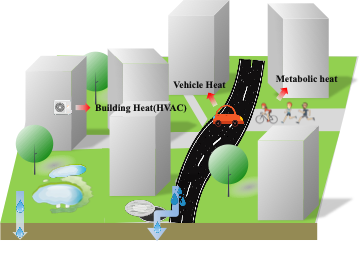
\includegraphics{Figures/城市模式/CoLM城市模式总体结构示意图.png}
\caption{CoLM城市模式总体结构示意图。}
\label{fig:CoLM城市模式总体结构示意图}
\end{figure}
}

建筑物底面考虑为正方形,边长为记为$L$。在已知$f_b$和$H/W$参数时,$L$可以计算为:
\begin{equation}
\frac{H}{L}=\frac{H}{W} \cdot \frac{1-\sqrt{f_{b}}}{\sqrt{f_{b}}}, \text { 即 } L=W \frac{\sqrt{f_{b}}}{1-\sqrt{f_{b}}}
\end{equation}
对于同一所在地城市覆盖,单栋建筑物几何参数一致,目前未考虑建筑物之间的几何差异,即以上参数代表为统计平均值。

在以下分模块公式推导中,下标约定如下:天空($s$),地面($g$,包括透水面$gper$和不透水面$gimp$),
墙面($w$,包括阳面墙$wsun$和阴面墙$wsha$),植被($v$)和屋顶$(r$)。$F$表示可视因子,例如$F_{gs}$表示从地面到天空的可视因子。
$S$表示阴影,$H/W$在推导过程中表示为$HW$,$H/L$表示为$HL$,总的直射入射和漫射入射太阳辐射能量通量采用单位能量1表示。

{
\begin{figure}[]
\centering
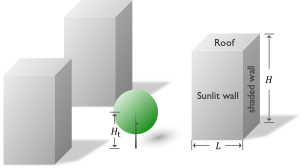
\includegraphics{Figures/城市模式/CoLM城市模式几何结构示意图.png}
\caption{CoLM城市模式几何结构示意图。}
\label{fig:CoLM城市模式几何结构示意图}
\end{figure}
}
\section{短波辐射传输}\label{短波辐射传输}
\subsection{无植被覆盖时短波辐射传输}\label{无植被覆盖时短波辐射传输}
太阳辐射直射照射时(太阳天顶角$\theta_s$),
建筑物群落在地面的阴影覆盖占比(被墙面遮挡的部分)计算为:
\begin{equation}\label{S_w}
S_{w}=1-\exp \left(-\frac{4}{\pi} \cdot \frac{f_{b}}{f_{g}} {HL} \cdot \tan \left(\theta_{s}\right)\right)
\end{equation}
阳面墙面积比例计算为:
\begin{equation}\label{f_wsun}
f_{wsun}=0.5 \cdot \frac{s_{w} f_{g}+f_{b}}{\frac{4}{\pi} f_{b} {HL} \tan \left(\theta_{s}\right)+f_{b}}
\end{equation}
阴面墙比例:
\begin{equation}\label{f_wsha}
f_{wsha}=1-f_{wsun}
\end{equation}
对于天空到墙面的可视因子$F_{sw}$,即天空漫射光源到达墙面的辐射部分,其计算类似与直射光在被墙面遮挡的面积比例:
\begin{equation}\label{f_Sw}
F_{S w}=1-\exp \left(-\frac{4}{\pi} \cdot \frac{f_{b}}{f_{g}} {HL} \cdot \tan \left(\theta_{s}^{*}\right)\right)
\end{equation}
其中$\theta_s^\ast$为漫射光情况下等效角度,可近似计算为:
\begin{equation}
\theta_{s}^{*}=\frac{53-10 \sqrt{\frac{f_{b}}{f_{g}} {HL}}}{180} \cdot \pi
\end{equation}
根据能量守恒,天空到达地面的可视因子$F_{sg}=1-F_{sw}$。
根据可视因子对称性,地面到达墙面和天空的可视因子$F_{gw}=F_{sw}$,$F_{gs}=F_{sg}$。
墙面到天空和地面的可视因子($F_{ws}$, $F_{wg}$)根据互易原理,满足如下关系:
\begin{equation}
F_{ws} \cdot 4 {HL} f_{b}=F_{s w} f_{g}
\end{equation}
\begin{equation}
F_{w g} \cdot 4 {HL} f_{b}=F_{s w} f_{g}
\end{equation}
由于太阳辐射在墙面垂直分布并不均匀,对上式进行简单调整,$F_{ws}$和$F_{wg}$计算为:
\begin{equation}
F_{ws}=0.75 F_{s w} \frac{f_{g}}{f_{b}} \frac{1}{2 {HL}}
\end{equation}
\begin{equation}
F_{w g}=0.25 F_{s w} \frac{f_{g}}{f_{b}} \frac{1}{2 {HL}}
\end{equation}
墙面到墙面的可视因子$F_{ww}=1-F_{ws}-F_{wg}$。

a. 直射入射太阳辐射

对于直射辐射太阳辐射,直射光到达阳面墙的辐射通量$E_{wsun}=S_w$,
到达阴面墙的辐射通量$E_{wsha}=0$,到达地面的辐射通量$E_g=1-E_{wsun}$,
其中$E_{gimp}=E_gf_{gimp}$,$E_{gper}=E_gf_{gper}$。
阳面墙、阴面墙、不透水面和透水面第一次散射辐射通量可分别计算为:
$E_{wsun}\alpha_w,E_{wsha}\alpha_w,E_{gimp}\alpha_{gimp},E_{gper}\alpha_{gper}$,
其中$\alpha$表示墙面、不透水面和透水面的反照率,不分区阳面和阴面,不区分漫射和直射照射,且反射后的辐射假设为漫射辐射。
设经过墙面地面之间多次散射,达到辐射平衡时的墙面和地面辐射出射通量为$M$,可建立如下辐射平衡方程:
\begin{landscape}
\begin{equation}
\begin{array}{l}
    M_{ {wsun }}=E_{wsun} \alpha_{w}+M_{wsun} F_{ww} f_{wsun} \alpha_{w}+M_{wsha} F_{ww} f_{wsun} \alpha_{w}+M_{gimp} F_{g w} f_{wsun} \alpha_{w}+M_{gper} F_{g w} f_{wsun} \alpha_{w} \\ 
    M_{wsha}=E_{wsha} \alpha_{w}+M_{wsha} F_{ww} f_{wsha} \alpha_{w}+M_{wsun} F_{ww} f_{wsha} \alpha_{w}+M_{gimp} F_{g w} f_{wsha} \alpha_{w}+M_{gper} F_{g w} f_{wsha} \alpha_{w} \\ 
    M_{gimp}=E_{gimp} \alpha_{gimp}+M_{wsun} F_{w g} f_{ gimp} \alpha_{gimp}+M_{wsha} F_{w g} f_{ gimp} \alpha_{gimp} \\ 
    M_{gper}=E_{gper} \alpha_{gper}+M_{wsun} F_{w g} f_{gper} \alpha_{gper}+M_{wsha} F_{w g} f_{gper} \alpha_{gper}
\end{array}
\end{equation}
通过整理得到:
\begin{equation}
\left(\begin{array}{cccc}1-F_{ww} f_{wsun} \alpha_{w} & -F_{ww} f_{wsun} \alpha_{w} & -F_{g w} f_{wsun} \alpha_{w} & -F_{g w} f_{wsun} \alpha_{w} \\
    -F_{ww} f_{wsha} \alpha_{w} & 1-F_{ww} f_{wsha} \alpha_{w} & -F_{g w} f_{wsha} \alpha_{w} & -F_{g w} f_{wsha} \alpha_{w} \\
    -F_{w g} f_{gimp} \alpha_{gimp} & -F_{w g} f_{gimp} \alpha_{gimp} & 1 & 0 \\ 
    -F_{w g} f_{gper} \alpha_{gper} & -F_{w g} f_{gper} \alpha_{gper} & 0 & 1\end{array}\right)
    \left(\begin{array}{l}M_{wsun} \\ M_{ {wsha }} \\ 
    M_{ gimp} \\ 
    M_{gper}\end{array}\right)=\left(\begin{array}{c}E_{wsun} \alpha_{w} \\
    E_{wsha} \alpha_{w} \\
    E_{gimp} \alpha_{ gimp} \\
    E_{gper} \alpha_{gper}\end{array}\right)
\end{equation}
\end{landscape}

简单表示为
\begin{equation}\label{mathbf_AX}
\mathbf{A X}=\mathbf{B}
\end{equation}
$\mathbf{A}$为辐射传输矩阵,$\mathbf{B}$为向量($E_{wsun}\alpha_w$,$E_{wsha}\alpha_w$,
$E_{gimp}\alpha_{gimp}$,$E_{gper}\alpha_{gper}$),
即墙面和地面第一次散射辐射通量。$\mathbf{X}$为求解变量组成的向量($M_{wsun}$,$M_{wsha}$,$M_{gimp}$,$M_{gper}$),
计算为:
\begin{equation}\label{mathbf_X}
\mathbf{X}=\mathbf{A}^{-1} \mathbf{B}
\end{equation}
矩阵$\mathbf{A}$是由已知变量组成的常数矩阵,可直接进行求逆计算,从而计算得到$\mathbf{X}$。墙面和地面的辐射吸收计算为:
\begin{equation}\label{s_wsun_wsha_gimp_gper_1}
\begin{array}{c}s_{wsun}=\frac{M_{wsun}}{\alpha_{w}}\left(1-\alpha_{w}\right) \\ 
    s_{wsha}=\frac{M_{wsha}}{\alpha_{w}}\left(1-\alpha_{w}\right) \\
    s_{gimp}=\frac{M_{gimp}}{\alpha_{gimp}}\left(1-\alpha_{gimp}\right) \\
    s_{gper}=\frac{M_{gper}}{\alpha_{gper}}\left(1-\alpha_{gper}\right)\end{array}
\end{equation}
注意,以上辐射吸收为总吸收量,其各自单面面积辐射吸收量修改为:
\begin{equation}\label{s_wsun_wsha_gimp_gper_2}
\begin{array}{c}s_{wsun}=\frac{f_{g}}{4 f_{wsun} \mathrm{HL} f_{b}} s_{wsun} \\ 
    s_{wsha}=\frac{f_{g}}{4 f_{wsha} \mathrm{HL} f_{b}} s_{wsha} \\ 
    s_{gimp}=\frac{1}{f_{gimp}} s_{gimp} \\ 
    s_{gper}=\frac{1}{f_{gper}} s_{gper}\end{array}
\end{equation}
不考虑屋顶时的城市反照率为:
\begin{equation}\label{alpha_u}
\alpha_{u}=M_{wsun} F_{ws}+M_{wsha} F_{ws}+M_{gimp} F_{gs}+M_{gper} F_{gs}
\end{equation}
屋顶的吸收计算为$s_{roof}=1-\alpha_{roof}$,考虑屋顶的城市反照率(\ref{alpha_u})修订为:
\begin{equation}\label{alpha_u2}
\alpha_{u}=\alpha_{{roof }} f_{b}+\alpha_{u} f_{g}
\end{equation}

b.漫射入射太阳辐射
对于漫射,计算过程与直射入射辐射过程基本类似,不同之处在于首次到达墙面和地面的辐射通量分别为:
$F_{sw}f_{wsun}$、$F_{sw}f_{wsha}$、$F_{sg}f_{gimp}$、$F_{sg}f_{gper}$,即公式(\ref{mathbf_AX})中的$\mathbf{B}$。
漫射入射辐射的传输矩阵同直射入射辐射情景,即A。其求逆后的结果可以直接用于漫射入射辐射,利用公式(\ref{mathbf_X})计算得到墙面和地面的辐射出射通量,
单位面积的辐射吸收和城市反照率同公式(\ref{alpha_u})和(\ref{alpha_u2}),在此不再列出。

\subsection{有植被覆盖时短波辐射传输}\label{有植被覆盖时短波辐射传输}
城市中考虑植被后的短波辐射传输过程是在无植被辐射传输的基础上,考虑植被在内的各组分之间的可视因子,
从而计算辐射平衡时的传输矩阵,采用类似的方法求解墙面、地面和植被的辐射吸收。
相比章节 \ref{无植被覆盖时短波辐射传输} 增加的部分为考虑植被在内的可视因子和阴影面积计算。

在植被树冠中心高度$h_v$处,墙面的阴影比例可根据公式(\ref{S_w})计算,利用$\frac{H-h_v}{H}$代替$HL$,记为$S_w^\prime$,即
\begin{equation}
S_{w}^{\prime}=1-\exp \left(-\frac{4}{\pi} \cdot \frac{f_{b}}{f_{g}} \frac{H-h_{v}}{H} \cdot \tan \left(\theta_{s}\right)\right)
\end{equation}
假设该阴影部分与植被覆盖$f_v$随机重叠,则植被被阴影遮挡的面积比例为$f_vS_w^\prime$,未覆盖的植被覆盖面积占比为$f_v^\prime=f_v-f_vS_w^\prime$。
该未被覆盖植被在整个城市覆盖区域的阴影覆盖$S_v$可根据公式(\ref{S_area})计算得到。将其覆盖比例转化为地面所占比例为:
\begin{equation}\label{S_v2}
S_{v}=S_{v} / f_{g}
\end{equation}

假设墙面在地面的阴影占比与植被的阴影随机重叠,则重叠部分占比$S_{vw}$计算为:
\begin{equation}
S_{v w}=S_{v}\left(S_{w}-S_{w}^{\prime}\right)
\end{equation}
该重叠部分假设全部为植被遮挡墙面部分。在地面覆盖区域,墙面的阴影占比修正为:
\begin{equation}\label{S_w2}
S_{w}=S_{w}-S_{v w}
\end{equation}
阴面墙和阳面墙的面积占比计算同公式(\ref{f_wsun})和(\ref{f_wsha})。

在不考虑植被存在时,可视因子$F_{sw}$, $F_{sg}$, $F_{gw}$, $F_{gs}$, $F_{ws}$, $F_{wg}$ 和 $F_{ww}$的
计算同章节 \ref{无植被覆盖时短波辐射传输},下面需要考虑植被的遮挡,对以上可视因子进行修改,并添加植被到各个面的可视因子。

同公式(\ref{S_v2})和(\ref{S_w2}),计算在漫射等效角度下的墙面和植被在地面的“阴影”占比(辐射遮挡) $S_w^\ast$和$S_v^\ast$,
利用公式(\ref{f_Sw})进行计算,则天空到达植被($F_{sv}$)、天空通过植被到墙面($F_{svw}$),以及天空通过植被到达地面的可视因子($F_{svg}$)分别计算为:
\begin{equation}\label{F_sv_svw_svg}
\begin{array}{c}F_{s v}=S_{v}^{*} \\ F_{s v w}=S_{v w}^{*} \\ F_{s v g}=F_{s v}-F_{s v w}\end{array}
\end{equation}
同理,地面到达植被($F_{gv}$)、地面通过植被到天空($F_{gvs}$),以及地面通过植被到达天空的可视因子($F_{gvs}$)可类似公式(\ref{F_sv_svw_svg})计算。

根据可视因子计算互易性原理,植被到天空、地面和墙面的可视因子计算为:
\begin{equation}
F_{vs}=F_{sv} \frac{f_g}{4 f_v}
\end{equation}
\begin{equation}
F_{vg}=F_{gv} \frac{f_g}{4 f_v}
\end{equation}
从而:
\begin{equation}
F_{v w}=1-F_{v s}-F_{v g}
\end{equation}
同理,根据互易性原理,$F_{wv}$计算为:
\begin{equation}
F_{w v}=F_{v w} \frac{f_{v}}{f_{b} \cdot {HL}}
\end{equation}
假设墙面通过植被到达墙面、天空和地面的可视因子与墙面到达相应各面的可视因子成正比,即:
\begin{equation}
F_{wvw}: F_{wvs}: F_{wvg}=F_{ww}: f_{1} F_{ws}: f_{2} F_{w g}
\end{equation}
其中$f_1=h_v/H$,$f_2=\left(H-h_v\right)/H$。根据能量守恒:
\begin{equation}
F_{wvw}+F_{wvs}+F_{wvg}=F_{w v}
\end{equation}
联合以上两式联立求解可得到:
\begin{equation}
F_{wvw}=\frac{F_{w v} F_{ww}}{F_{ww}+f_{1} F_{ws}+f_{2} F_{w g}}
\end{equation}
\begin{equation}
F_{wvs}=f_{1} \frac{F_{ws}}{F_{ww}} F_{wvw}
\end{equation}
\begin{equation}
F_{wvg}=f_{2} \frac{F_{w g}}{F_{ww}} F_{wvw}
\end{equation}
在此基础上,可以计算得到考虑植被影响的天空、墙面和地面之间的可视因子,
其中天空到墙面和地面的可视因子$F_{sw}^\prime$, $F_{sg}^\prime$计算为:
\begin{equation}
F_{s w}^{\prime}=F_{s w}-F_{s v w}+F_{s v w} T_{d}
\end{equation}
\begin{equation}
F_{s g}^{\prime}=F_{s g}-F_{s v g}+F_{s v g} T_{d}
\end{equation}
其中$T_d$为单棵球形树冠直射透射率,利用公式(\ref{T_ds_tau})计算。
地面到达墙面和天空的可视因子$F_{gw}^\prime$, $F_{gs}^\prime$计算为:
\begin{equation}
F_{g w}^{\prime}=F_{g w}-F_{g v w}+F_{g v w} T_{d}
\end{equation}
\begin{equation}
F_{gs}^{\prime}=F_{gs}-F_{g v s}+F_{g v s} T_{d}
\end{equation}
墙面到达地面、墙面和天空的可视因子$F_{wg}^\prime$, $F_{ww}^\prime$, $F_{ws}^\prime$计算为:
\begin{equation}
F_{w g}^{\prime}=F_{w g}-F_{wvg}+F_{wvg} T_{d}
\end{equation}
\begin{equation}
F_{ww}^{\prime}=F_{ww}-F_{wvw}+F_{wvw} T_{d}
\end{equation}
\begin{equation}
F_{ws}^{\prime}=F_{ww}-F_{wvs}+F_{wvs} T_{d}
\end{equation}

a. 直射入射太阳辐射

对于直射辐射太阳辐射,直射光到达阳面墙的辐射通量$E_{wsun}=S_w$,到达阴面墙的辐射通量$E_{wsha}=S_{vw}T_d$,
到达地面的辐射通量$E_g=1-S_w-S_v+\left(S_v-S_{vw}\right)T_d$,其中$E_{gimp}=E_gf_{gimp}$,$E_{gper}=E_gf_{gper}$,
$E_v=S_v$。阳面墙、阴面墙、不透水面、透水面和植被第一次散射辐射通量可分别计算为:$E_{wsun}\alpha_w$,$E_{wsha}\alpha_w$,
$E_{gimp}\alpha_{gimp}$,$E_{gper}\alpha_{gper}$,$E_v\alpha_v$,
其中$\alpha$表示反照率(对于植被表示所有向外散射辐射),不分区阳面和阴面,不区分漫射和直射照射,
且反射后的辐射假设为漫射辐射。假设经过墙面、地面和植被之间多次散射,达到辐射平衡时的墙面和地面辐射出射通量为$M$,
利用各组分之间的可视因子,可建立如下辐射平衡方程:
\begin{landscape}
\begin{equation}
\begin{array}{l}M_{wsun}=E_{wsun} \alpha_{w}+M_{wsun} F_{ww}^{\prime} f_{wsun} \alpha_{w}+M_{wsha} F_{ww}^{\prime} f_{wsun} \alpha_{w}+M_{gimp} F_{g w}^{\prime} f_{wsun} \alpha_{w}+M_{gper} F_{g w}^{\prime} f_{wsun} \alpha_{w}+M_{v} F_{v w} f_{wsun} \alpha_{w} \\ M_{wsha}=E_{wsha} \alpha_{w}+M_{wsha} F_{ww}^{\prime} f_{wsha} \alpha_{w}+M_{wsun} F_{ww}^{\prime} f_{wsha} \alpha_{w}+M_{gimp} F_{g w}^{\prime} f_{wsha} \alpha_{w}+M_{gper} F_{g w}^{\prime} f_{wsha} \alpha_{w}+M_{v} F_{v w} f_{wsha} \alpha_{w} \\ M_{gimp}=E_{gimp} \alpha_{gimp}+M_{wsun} F_{w g}^{\prime} f_{gimp} \alpha_{gimp}+M_{wsha} F_{w g}^{\prime} f_{gimp} \alpha_{gimp}+M_{v} F_{v g} f_{gimp} \alpha_{gimp} \\ M_{gper}=E_{gper} \alpha_{gper}+M_{wsun} F_{w g}^{\prime} f_{gper} \alpha_{gper}+M_{wsha} F_{w g}^{\prime} f_{gper} \alpha_{gper}+M_{v} F_{v g} f_{gper} \alpha_{gper} \\ M_{v}=E_{v} \alpha_{v}+M_{wsun} F_{w v} \alpha_{v}+M_{wsha} F_{w v} \alpha_{v}+M_{gimp} F_{g v} \alpha_{v}+M_{gper} F_{g v} \alpha_{v}\end{array}
\end{equation}
整理之后简化为:
\begin{equation}
\left(\begin{array}{ccccc}1-F_{ww}^{\prime} f_{wsun} \alpha_{w} & -F_{ww}^{\prime} f_{wsun} \alpha_{w} & -F_{g w}^{\prime} f_{wsun} \alpha_{w} & -F_{g w}^{\prime} f_{wsun} \alpha_{w} & -F_{v w} f_{wsun} \alpha_{w} \\ -F_{ww}^{\prime} f_{wsha} \alpha_{w} & 1-F_{ww}^{\prime} f_{wsha} \alpha_{w} & -F_{g w}^{\prime} f_{wsha} \alpha_{w} & -F_{g w}^{\prime} f_{wsha} \alpha_{w} & -F_{v w} f_{wsha} \alpha_{w} \\ -F_{w g}^{\prime} f_{gimp} \alpha_{gimp} & -F_{w g}^{\prime} f_{gimp} \alpha_{gimp} & 1 & 0 & -F_{v g} f_{gimp} \alpha_{gimp} \\ -F_{w g}^{\prime} f_{gper} \alpha_{gper} & -F_{w g}^{\prime} f_{gper} \alpha_{gper} & 0 & 1 & -F_{v g} f_{gper} \alpha_{gper} \\ -F_{w v} \alpha_{v} & -F_{w v} \alpha_{v} & -F_{g v} \alpha_{v} & -F_{g v} \alpha_{v} & 1\end{array}\right)\left(\begin{array}{c}M_{wsun} \\ M_{wsha} \\ M_{gimp} \\ M_{gper} \\ M_{v}\end{array}\right)=\left(\begin{array}{c}E_{wsun} \alpha_{w} \\ E_{wsha} \alpha_{w} \\ E_{gimp} \alpha_{gimp} \\ E_{gper} \alpha_{gper} \\ E_{v} \alpha_{v}\end{array}\right)
\end{equation}
\end{landscape}
方程求解同公式(\ref{mathbf_X}),阳面墙、阴面墙、不透水面和透水面的辐射总吸收及单位面积吸收同式(\ref{s_wsun_wsha_gimp_gper_1})和(\ref{s_wsun_wsha_gimp_gper_2})。植被的吸收计算类似,表达式为:
\begin{equation}
s_{v}=\frac{M_{v}}{a_{v}}\left(1-a_{v}-T_{d}\right)
\end{equation}
若考虑单位面积植被覆盖吸收辐射量,则$s_v$修订为:
\begin{equation}
s_{v}=\frac{f_{g}}{f_{v}} s_{v}
\end{equation}
不考虑屋顶时的城市反照率为:
\begin{equation}\label{alpha_u_a1}
\alpha_{u}=M_{wsun} F_{ws}^{\prime}+M_{wsha} F_{ws}^{\prime}+M_{gimp} F_{gs}^{\prime}+M_{gper} F_{gs}^{\prime}+M_{v} F_{v s}
\end{equation}
屋顶的吸收计算为$s_{roof}=1-\alpha_{roof}$,考虑屋顶的城市反照率(\ref{alpha_u_a1})修订为:
\begin{equation}
\alpha_{u}=\alpha_{roof} f_{b}+\alpha_{u} f_{g}
\end{equation}

b. 漫射入射太阳辐射

对于漫射,计算过程与直射入射辐射过程基本类似,不同之处在于首次到达墙面、地面和植被的辐射通量分别为:$F_{sw}^\prime f_{wsun}$、
$F_{sw}^\prime f_{wsha}$、$F_{sg}^\prime f_{gimp}$、$F_{sg}^\prime f_{gper}$和$F_{sv}$。
漫射入射辐射的传输矩阵同直射入射辐射情景。其求逆后的结果可以直接用于漫射入射辐射,各组分的辐射吸收和反照率计算过程在此不再赘述。 
\section{长波辐射传输}
\subsection{无植被覆盖时长波辐射传输}
无植被时的长波辐射传输类似与无植被时短波辐射传输时的漫射入射情景(长波辐射近似为漫射光源处理)。首次达到各组分表面的长波辐射通量为:
\begin{equation}
\begin{aligned} I_{wsun} &=L_{W} F_{s w} f_{wsun} \\ I_{wsha} &=L_{W} F_{s w} f_{wsha} \\ I_{gimp} &=L_{W} F_{s g} f_{gimp} \\ I_{gper} &=L_{W} F_{s g} f_{gper} \end{aligned}
\end{equation}
第一次反射的长波辐射通量依次分别为:
\begin{equation}
\begin{array}{c}I_{wsun}\left(1-\varepsilon_{w}\right) \\ I_{wsha}\left(1-\varepsilon_{w}\right) \\ I_{gimp}\left(1-\varepsilon_{gimp}\right) \\ I_{gper}\left(1-\varepsilon_{gper}\right)\end{array}
\end{equation}
上式中$\varepsilon$表示发射率,$\varepsilon_w$,$\varepsilon_{gimp}$,$\varepsilon_{gper}$为已知变量。各组分表面向外发射的长波辐射量为:
\begin{equation}
\begin{array}{c}4 f_{wsun} \mathrm{HL} \times \frac{f_{b}}{f_{g}} \times \sigma \varepsilon_{w} T_{wsun}^{4} \\
4 f_{wsha} \mathrm{HL} \times \frac{f_{b}}{f_{g}} \times \sigma \varepsilon_{w} T_{wsha}^{4} \\
\sigma \varepsilon_{gimp} T_{gimp}^{4} f_{gimp} \\
\sigma \varepsilon_{gper} T_{gper}^{4} f_{gper}\end{array}
\end{equation}
$T$表示温度,$\sigma$为斯蒂芬-玻尔兹曼常数。类似与短波辐射传输,可以构建辐射平衡方程:
\begin{landscape}
\begin{equation}
    \begin{aligned}
        L_{wsun}^{\uparrow}=I_{wsun}\left(1-\varepsilon_{w}\right)+L_{wsun}^{\uparrow} F_{ww} f_{wsun}\left(1-\varepsilon_{w}\right)+L_{wsha}^{\uparrow} F_{ww} f_{wsun}\left(1-\varepsilon_{w}\right)+L_{gimp}^{\uparrow} F_{g w} f_{wsun}\left(1-\varepsilon_{w}\right)\\+L_{gper}^{\uparrow} F_{g w} f_{wsun}\left(1-\varepsilon_{w}\right)+4 f_{wsun} H L * \frac{f_{b}}{f_{g}} * \sigma \varepsilon_{w} T_{wsun}^{4}\\
        L_{wsha}^{\uparrow}=I_{wsha}\left(1-\varepsilon_{w}\right)+L_{wsha}^{\uparrow} F_{ww} f_{wsha}\left(1-\varepsilon_{w}\right)+L_{wsun}^{\uparrow} F_{ww} f_{wsha}\left(1-\varepsilon_{w}\right)+L_{gimp}^{\uparrow} F_{g w} f_{wsha}\left(1-\varepsilon_{w}\right)\\+L_{gper}^{\uparrow} F_{g w} f_{wsha}\left(1-\varepsilon_{w}\right)+4 f_{wsha} H L * \frac{f_{b}}{f_{g}} * \sigma \varepsilon_{w} T_{wsha}^{4}\\
        L_{gimp}^{\uparrow}=I_{gimp}\left(1-\varepsilon_{gimp}\right)+L_{wsun}^{\uparrow} F_{w g} f_{gimp}\left(1-\varepsilon_{gimp}\right)+L_{wsha}^{\uparrow} F_{w g} f_{gimp}\left(1-\varepsilon_{gimp}\right)+\sigma \varepsilon_{gimp} T_{gimp}^{4} f_{gimp}\\
        L_{gper}^{\uparrow}=I_{gper}\left(1-\varepsilon_{gper}\right)+L_{wsun}^{\uparrow} F_{w g} f_{gper}\left(1-\varepsilon_{gper}\right)+L_{wsha}^{\uparrow} F_{w g} f_{gper}\left(1-\varepsilon_{gper}\right)+\sigma \varepsilon_{gper} T_{gper}^{4} f_{gper}
    \end{aligned}
\end{equation}
其中$L^\uparrow$表示各组分表面总的向外长波辐射量(反射部分+自身发射部分)。经过整理,可得:
\begin{equation}
\begin{aligned}
\left(\begin{matrix}1-F_{ww}f_{wsun}\left(1-\varepsilon_w\right)&-F_{ww}f_{wsun}\left(1-\varepsilon_w\right)&-F_{gw}f_{wsun}\left(1-\varepsilon_w\right)&-F_{gw}f_{wsun}\left(1-\varepsilon_w\right)\\-F_{ww}f_{wsha}\left(1-\varepsilon_w\right)&1-F_{ww}f_{wsha}\left(1-\varepsilon_w\right)&-F_{gw}f_{wsha}\left(1-\varepsilon_w\right)&-F_{gw}f_{wsha}\left(1-\varepsilon_w\right)\\-F_{wg}f_{gimp}\left(1-\varepsilon_{gimp}\right)&-F_{wg}f_{gimp}\left(1-\varepsilon_{gimp}\right)&1&0\\-F_{wg}f_{gper}\left(1-\varepsilon_{gper}\right)&-F_{wg}f_{gper}\left(1-\varepsilon_{gper}\right)&0&1\\\end{matrix}\right)
\left(\begin{matrix}L_{wsun}^\uparrow\\L_{wsha}^\uparrow\\L_{gimp}^\uparrow\\L_{gper}^\uparrow\\\end{matrix}\right)\\
=\left(\begin{matrix}I_{wsun}\left(1-\varepsilon_w\right)+2f_{wsun}\frac{\sigma\varepsilon_wT_{wsun}^4H}{W}\\I_{wsha}\left(1-\varepsilon_w\right)+2f_{wsha}\frac{\sigma\varepsilon_wT_{wsha}^4H}{W}\\I_{gimp}\left(1-\varepsilon_{gimp}\right)+\sigma\varepsilon_{gimp}T_{gimp}^4f_{gimp}\\I_{gper}\left(1-\varepsilon_{gper}\right)+\sigma\varepsilon_{gper}T_{gper}^4f_{gper}\\\end{matrix}\right)
\end{aligned}
\end{equation}
\end{landscape}

以上方程也可以记为矩阵形式:
\begin{equation}
\mathbf{A X}=\mathbf{B}
\end{equation}
求解以上方程得到$\mathbf{X}$,各组分表面长波净辐射量为:
\begin{equation}\label{L_wsun_wsha_gimp_pger_1}
\begin{array}{c}L_{wsun}=\frac{\varepsilon L_{wsun}^{\uparrow}-4 f_{wsun} \mathrm{HL} * \frac{f_{b}}{f_{g}} * \sigma \varepsilon_{w} T_{wsun}^{4}}{1-\varepsilon_{w}} \\ L_{wsha}=\frac{\varepsilon L_{wsha}^{\uparrow}-4 f_{wsha} \mathrm{HL} * \frac{f_{b}}{f_{g}} * \sigma \varepsilon_{w} T_{wsha}^{4}}{1-\varepsilon_{w}} \\ L_{gimp}=\frac{\varepsilon L_{w gimp}^{\uparrow}-\sigma \varepsilon_{gimp} T_{gimp}^{4} f_{gimp}}{1-\varepsilon_{gimp}} \\ L_{p g e r}=\frac{\varepsilon L_{w gper}^{\uparrow}-\sigma \varepsilon_{gper} T_{gper}^{4} f_{gper}}{1-\varepsilon_{gper}}\end{array}
\end{equation}
转化为单位面积净辐射时上式修改为:
\begin{equation}\label{L_wsun_wsha_gimp_pger_2}
\begin{array}{c}L_{wsun}=\frac{f_{g}}{4 f_{wsun} \mathrm{HL} f_{b}} L_{wsun} \\ L_{wsha}=\frac{f_{g}}{4 f_{wsha} \mathrm{HL} f_{b}} L_{wsha} \\ L_{gimp}=\frac{1}{f_{gimp}} L_{gimp} \\ L_{gper}=\frac{1}{f_{gper}} L_{gper}\end{array}
\end{equation}
在不考虑屋顶时的向外长波辐射通量计算为:
\begin{equation}
L^{\uparrow}=L_{wsun}^{\uparrow} F_{ws}+L_{wsha}^{\uparrow} F_{ws}+L_{gimp}^{\uparrow} F_{gs}+L_{gper}^{\uparrow} F_{gs}
\end{equation}


\subsection{有植被覆盖时长波辐射传输}\label{有植被覆盖时长波辐射传输}
考虑植被覆盖时的长波辐射计算类似于有植被覆盖时的短波辐射传输,根据之前介绍的无植被时长波辐射传输平衡方程,可以写出有植被覆盖时: 
\begin{landscape}
\begin{equation}
    \begin{aligned}
    L_{{wsun }}^{\uparrow}=I_{{wsun }}\left(1-\varepsilon_{w}\right)+L_{wsun}^{\uparrow} F_{ww}^{\prime} f_{wsun}\left(1-\varepsilon_{w}\right)+L_{wsha}^{\uparrow} F_{ww}^{\prime} f_{wsun}\left(1-\varepsilon_{w}\right)+L_{gimp}^{\uparrow} F_{g w}^{\prime} f_{wsun}\left(1-\varepsilon_{w}\right)+L_{gper}^{\uparrow} F_{g w}^{\prime} f_{wsun}\left(1-\varepsilon_{w}\right)\\+L_{v}^{\uparrow} F_{v w} f_{wsun}\left(1-\varepsilon_{w}\right)+4 f_{wsun} H L * \frac{f_{b}}{f_{g}} * \sigma \varepsilon_{w} T_{wsun}^{4} \\
    L_{wsha}^{\uparrow}=I_{wsha}\left(1-\varepsilon_{w}\right)+L_{wsha}^{\uparrow} F_{ww}^{\prime} f_{wsha}\left(1-\varepsilon_{w}\right)+L_{wsun}^{\uparrow} F_{ww}^{\prime} f_{wsha}\left(1-\varepsilon_{w}\right)+L_{gimp}^{\uparrow} F_{g w}^{\prime} f_{wsha}\left(1-\varepsilon_{w}\right)+L_{gper}^{\uparrow} F_{g w}^{\prime} f_{wsha}\left(1-\varepsilon_{w}\right)\\+L_{v}^{\uparrow} F_{v w} f_{wsha}\left(1-\varepsilon_{w}\right)+4 f_{wsha} H L * \frac{f_{b}}{f_{g}} * \sigma \varepsilon_{w} T_{wsha}^{4}\\
    L_{gimp}^{\uparrow}=I_{gimp}\left(1-\varepsilon_{gimp}\right)+L_{wsun}^{\uparrow} F_{w g}^{\prime} f_{gimp}\left(1-\varepsilon_{gimp}\right)+L_{wsha}^{\uparrow} F_{w g}^{\prime} f_{gimp}\left(1-\varepsilon_{gimp}\right)+L_{v}^{\uparrow} F_{v g} f_{gimp}\left(1-\varepsilon_{gimp}\right)+\sigma \varepsilon_{gimp} T_{gimp}^{4} f_{gimp} \\
    L_{gper}^{\uparrow}=I_{gper}\left(1-\varepsilon_{gper}\right)+L_{wsun}^{\uparrow} F_{w g}^{\prime} f_{gper}\left(1-\varepsilon_{gper}\right)+L_{wsha}^{\uparrow} F_{w g}^{\prime} f_{gper}\left(1-\varepsilon_{gper}\right)+L_{v}^{\uparrow} F_{v g} f_{gper}\left(1-\varepsilon_{gper}\right)+\sigma \varepsilon_{{gpre }} T_{{gpre }}^{4} f_{{gpre }} \\
    L_{v}^{\uparrow}=4 f_{v} / f_{g} \sigma \varepsilon_{v} T_{v}^{4}
    \end{aligned}
\end{equation}
\end{landscape}

\begin{landscape}
上式中的$F$, $F^\prime$表示可视因子,同章节 \ref{有植被覆盖时短波辐射传输}。经过整理,可以得到:
\begin{equation}
    \begin{split}
    \left(\begin{matrix}1-\ F_{ww}^\prime f_{wsun}\left(1-\varepsilon_w\right)&-\ F_{ww}^\prime f_{wsun}\left(1-\varepsilon_w\right)&-F_{gw}^\prime f_{wsun}\left(1-\varepsilon_w\right)&-F_{gw}^\prime f_{wsun}\left(1-\varepsilon_w\right)&-F_{vw}f_{wsun}\left(1-\varepsilon_w\right)\\
    -\ F_{ww}^\prime f_{wsha}\left(1-\varepsilon_w\right)&1-\ F_{ww}^\prime f_{wsha}\left(1-\varepsilon_w\right)&-F_{gw}^\prime f_{wsha}\left(1-\varepsilon_w\right)&-F_{gw}^\prime f_{wsha}\left(1-\varepsilon_w\right)&-F_{vw}f_{wsha}\left(1-\varepsilon_w\right)\\
    -F_{wg}^\prime f_{gimp}\left(1-\varepsilon_{gimp}\right)&-F_{wg}^\prime f_{gimp}\left(1-\varepsilon_{gimp}\right)&1&0&-F_{vg}f_{gimp}\left(1-\varepsilon_{gimp}\right)\\
    -F_{wg}^\prime f_{gper}\left(1-\varepsilon_{gper}\right)&-F_{wg}^\prime f_{gper}\left(1-\varepsilon_{gper}\right)&0&1&-F_{vg}f_{gper}\left(1-\varepsilon_{gper}\right)\\
    0&0&0&0&1\\\end{matrix}\right)\cdot \\
    \left(\begin{matrix}L_{wsun}^\uparrow\\L_{wsha}^\uparrow\\L_{gimp}^\uparrow\\L_{gper}^\uparrow\\L_v^\uparrow\\\end{matrix}\right)
    =\left(\begin{matrix}I_{wsun}\left(1-\varepsilon_w\right)+4f_{wsun}HL \times \frac{f_b}{f_g} \times \sigma\varepsilon_wT_{wsun}^4 \\
        I_{wsha}\left(1-\varepsilon_w\right)+4f_{wsha}HL \times \frac{f_b}{f_g} \times \sigma\varepsilon_wT_{wsha}^4  \\
        I_{gimp}\left(1-\varepsilon_{gimp}\right)+\sigma\varepsilon_{gimp}T_{gimp}^4f_{gimp} \\
        I_{gper}\left(1-\varepsilon_{gper}\right)+\sigma\varepsilon_{gper}T_{gper}^4f_{gper}\\
        4f_v/f_g\sigma\varepsilon_vT_v^4\\\end{matrix}\right)
    \end{split}
\end{equation}
\end{landscape}

求解以上方程,墙面和地面长波净辐射及单位面积净辐射计算公式同(\ref{L_wsun_wsha_gimp_pger_1})和(\ref{L_wsun_wsha_gimp_pger_2})。植被净辐射吸收为:
\begin{equation}
L_{v}=\left(L_{wsun}^{\uparrow} F_{w v}+L_{wsha}^{\uparrow} F_{w v}+L_{gimp}^{\uparrow} F_{g v}+L_{gper}^{\uparrow} F_{g v}+L_{W} F_{s v}\right) \varepsilon_{v}-4 f_{v} / f_{g} \sigma \varepsilon_{v} T_{v}^{4}
\end{equation}
植被单位面积覆盖长波净辐射修改为:
\begin{equation}
L_{v}=\frac{f_{g}}{f_{v}} L_{v}
\end{equation}
不考虑屋顶时城市总的向外长波辐射计算为:
\begin{equation}
L^{\uparrow}=L_{wsun}^{\uparrow} F_{ws}^{\prime}+L_{wsha}^{\uparrow} F_{ws}^{\prime}+L_{gimp}^{\uparrow} F_{gs}^{\prime}+L_{gper}^{\uparrow} F_{gs}^{\prime}+L_{v}^{\uparrow} F_{v s}
\end{equation}
\section{湍流交换过程}
城市湍流交换过程与三维植被湍流交换过程类似,计算屋顶、墙面(阴、阳面)、地面和植被的感热、潜热交换量,
同样是基于相似性理论,建立每层(等效高度)通量守恒方程,联立求解。不同之处在于其粗糙度、迎风面积指数、
零平面位移高度、风速/湍流交换系数衰减系数、建筑表面边界层阻抗计算与植被有所不同。
下面就无植被覆盖和有植被覆盖时对不同于自然植被湍流交换过程的部分进行简要说明。
\subsection{无植被覆盖时湍流交换过程}
建筑物的零平面位移高度采用~\citet{macdonald1998improved}方案:
\begin{equation}
\frac{d}{H}=1+A^{-f_{b}}\left(f_{b}-1\right)
\end{equation}
其中$A$取值为4.43。迎风面积指数可以计算为:
\begin{equation}
\lambda_{f}=\frac{2}{\pi} \cdot H L \cdot f_{b} \int_{0}^{\frac{\pi}{2}}(\cos \theta+\sin \theta) d \theta=\frac{4}{\pi} \cdot H L f_{b}
\end{equation}
粗糙度计算为:
\begin{equation}
\frac{z_{0}}{H}=\left(1-\frac{d}{H}\right) \exp \left[-\left(0.5 \frac{c_{D}}{\kappa^{2}}\left(1-\frac{d}{H}\right) \lambda_{f}\right)^{-0.5}\right]
\end{equation}
其中$C_D=1.2$,$\kappa=0.4$为 von K\'arman 常数。

城市冠层内的风速和湍流交换系数同样假设为指数衰减,但衰减系数与植被不同,
采用\citet{masson2000physically}方案,计算为0.5$HW$。建筑物(屋顶、墙面)边界层阻抗$r_b$计算为\citep{oleson2008urban}:
\begin{equation}
r_{b}=\frac{\rho_{a} c_{p}}{11.8+4.2 u_{e f f}}
\end{equation}
其中$u_{eff}$表示屋顶高度/墙面交换高度的等效风速值,$\rho_a$表示空气密度,$C_p$表示干空气定压比热容。

以上为主要区别于三维植被湍流交换过程计算的部分,整个正式湍流交换计算阻抗网络如图~\ref{fig:无植被覆盖时城市湍流交换阻抗示意图} 所示。
湍流交换计算过程与三维植被湍流交换方案类似,先通过相似性理论计算屋顶高度风速和湍流交换系数;
然后根据指数衰减假设,参考三维植被湍流交换方案~\citep{dai2019different},
根据公式(\ref{uz})和(\ref{Kz})计算风速和湍流交换系数在城市冠层内部剖面。屋顶的等效风速即为H高度时的风速,
墙面的等效风速为H到地面的平均风速,通过风速剖面积分计算得到。同理,屋顶与墙面等效交换高度之间的动力学交换阻抗,
以及墙面等效交换高度与地面之间的动力学阻抗$r_d$均是通过对交换系数剖面积分计算得到(公式(\ref{r_d1}))。
同多层植被湍流交换计算一样,对上图所示的屋顶和墙面等效交换高度建立感热和潜热通量守恒方程,
迭代求解其高度处的空气温度、湿度以及相似性理论交换长度(即空气不稳定程度)。
因为这部分过程与三维植被湍流交换过程完全一致,在此不再阐述。
{
\begin{figure}[]
\centering
\includegraphics{Figures/城市模式/无植被覆盖时城市湍流交换阻抗示意图.png}
\caption{无植被覆盖时城市湍流交换阻抗示意图。}
\label{fig:无植被覆盖时城市湍流交换阻抗示意图}
\end{figure}
}


\subsection{有植被覆盖式湍流交换过程}
有植被覆盖时的湍流交换网络如图~\ref{fig:有植被覆盖时城市湍流交换阻抗示意图} 所示,
其计算过程与无植被覆盖时类似,不同之处在于新增植被组分。因此,在建立通量守恒方程式时,
需要考虑植被的感热、潜热交换,涉及到植被光合作用(蒸腾)和长波辐射吸收计算。
光合作用过程同自然植被光合作用过程,长波辐射吸收计算在章节 \ref{有植被覆盖时长波辐射传输} 已给出。
在实际计算过程中,可根据植被与建筑物高度差异,视情况分为两层或三层等效交换(三层时,即植被单独考虑为一层)。
整个过程也是迭代求解,但此时需要新增迭代求解变量叶片温度,其他过程同无植被覆盖时湍流交换过程。
{
\begin{figure}[]
\centering
\includegraphics{Figures/城市模式/有植被覆盖时城市湍流交换阻抗示意图.png}
\caption{有植被覆盖时城市湍流交换阻抗示意图。}
\label{fig:有植被覆盖时城市湍流交换阻抗示意图}
\end{figure}
}


\section{城市温度传导计算}
城市内透水面、不透水面、墙面和屋顶的温度传导计算以自然界土壤温度传导计算为基础,基本过程一致,下面重点介绍城市的不同之处。

\subsection{透水面温度计算}
城市透水面即为土壤,与自然界土壤的热传递计算一致 (分层方案与土壤一致,
土壤热力参数也从全球数据中读取),只是上表面接收的短波、长波辐射及湍流交换通量(感热、潜热)由城市相应模块求解得到。

\subsection{不透水面温度计算}
不透水面的温度传导计算与透水面最大的不同之处在于需要将不透水面层的热力属性(导热率和热容)替换掉所在层的土壤热力属性。
另外在有雪、冰和水存在时,需要对第一层不透水面的热容进行订正。不透水面不考虑水分在内部的传递,相变过程只考虑第一层及以上积雪覆盖。

\subsection{墙面温度计算}
墙面(包括阴面墙、阳面墙)厚度从外部数据读取,同土壤一样,也分为10层,每层厚度一样,其热力参数从外部数据读取。
不同于透水面/不透水面,墙面不考虑积水、积雪覆盖,因此其热力属性完全由自身材料决定,同时也不考虑水传递、相变过程和潜热交换。

另一个不同之处在于最里(下)层的热量交换设置,对于土壤、不透水面,考虑最下一层无热量交换,但对于墙壁,
考虑室内墙壁表面温度与最里层墙壁的热量交换。除此之外,其他方面及其求解过程与土壤温度类似。


\subsection{屋顶温度计算}
屋顶的分层方案与墙壁一致。温度传递类似于墙面,但考虑屋顶积雪、积水覆盖时对屋顶第一层热力属性的影响,同不透水面。
同时最里层屋顶与室内屋顶表面温度考虑热量交换,相变过程只考虑第一层屋顶。


\section{城市水文过程}
对城市水文过程考虑主要分为三类:1) 透水面;2) 屋顶和不透水面;3) 城市水体。

对于透水面的处理同土壤水过程,计算产流和土壤水传输。对于城市水体,采用湖泊方案进行模拟。对于屋顶和不透水面,
考虑积雪和积水过程,类似与土壤积雪过程,但第一层为不透水面,液态水的最大承载量为不超过设定的值(max ponding),
超过的部分均当成地表产流处理。

由于目前城市水文过程比较简单,相应过程在土壤和湖泊模拟部分均有描述,在此不再赘述。


\section{城市人为热模拟}

\subsection{建筑能耗模型}
CoLM建筑物能耗模型如图~\ref{fig:建筑能耗模型示意图} 所示,同样是基于三维城市建筑群落结构假设,其过程类似于CLM5.0建筑能耗模型。
模型考虑墙体、屋顶的热传导过程,同时考虑室内空气与内墙壁、屋顶和室外的热量交换。根据室内设定的最高、
最低参考温度,来计算空调对应能耗,以感热的形式增加到湍流交换计算的源项中。
首先计算热交换通量并建立能量平衡方程,进而求解室内温度$T_{room}$,室内墙壁表面空气温度$T_{wsun,in}$,$T_{wsua,in}$和室内屋顶表面空气温度$T_{roof,in}$。
通量交换包括最里层墙壁/屋顶与屋内墙壁/屋顶表面空气热量交换,屋内墙壁/屋顶表面空气与室内空气热量交换以及室内空气与室外空气热量交换,通量平衡方程为: 
{
\begin{figure}[]
\centering
\includegraphics{Figures/城市模式/建筑能耗模型示意图.png}
\caption{建筑能耗模型示意图。}
\label{fig:建筑能耗模型示意图}
\end{figure}
}

\begin{landscape}
\begin{equation}
    \begin{array}{l}
        \begin{split}
        0.5 h_{{roof }, c v}\left(t_{{roof }, { in }}-t_{{room }}\right)+0.5 h_{{roof }, c v}\left(t_{{roof,in }}^{\prime}-t_{{room }}^{\prime}\right)=0.5 h_{{roof }, t k}\left(T_{{roof }, n}-T_{{roof }, { in }}\right)+0.5 h_{{roof }, t k}\left(T_{{roof }, n}-T_{{roof,in }}^{\prime}\right) \\
        0.5 h_{{wsun, }, v}\left(t_{{wsun,in }}-t_{{room }}\right)+0.5 h_{{wsun, cv }}\left(t_{wsun, i n}^{\prime}-t_{{room }}^{\prime}\right)=0.5 h_{{wsun,tk }}\left(T_{{wsun, } n}-T_{{wsun,in }}\right)+0.5 h_{{roof,tk }}\left(T_{{wsun, } n}-T_{{wsun,in }}^{\prime}\right)\\
        0.5 h_{wsha, c v}\left(t_{wsha, i n}-t_{{room }}\right)+0.5 h_{wsha, c v}\left(t_{wsha, i n}^{\prime}-t_{{room }}^{\prime}\right)=0.5 h_{wsha, t k}\left(T_{wsha, n}-T_{{roof }, i n}\right)+0.5 h_{wsha, t k}\left(T_{wsha, n}-T_{wsha, i n}^{\prime}\right)\\
        H \rho_{a} C_{p} \frac{T_{{room }}^{\prime}-T_{{room }}}{\Delta t}
        =\frac{ACH}{3600} H \rho_{a} C_{p}\left(T_{a f}-T_{{room }}^{\prime}\right)+0.5 h_{{roof }, c v}\left(t_{{roof }, { in }}-t_{{room }}\right)+0.5 h_{{roof }, c v}\left(t_{{roof }, { in }}^{\prime}-t_{{room }}^{\prime}\right)\\
        +0.5 h_{wsun, c v}\left(t_{wsun, i n}-t_{{room }}\right) f_{{wsun }}+0.5 h_{wsun, c v}\left(t_{wsun, i n}^{\prime}-t_{{room }}^{\prime}\right) f_{wsun} \\
        +0.5 h_{wsha, c v}\left(t_{wsha, i n}-t_{{room }}\right) f_{wsha}+0.5 h_{wsha, c v}\left(t_{wsha, i n}^{\prime}-t_{r o o m}^{\prime}\right) f_{wsha}
        \end{split}
    \end{array}
\end{equation}
以上方程组可写成矩阵形式:
\begin{equation}
    \begin{split}
\left(\begin{array}{cccc}0.5 h_{r o o f, c v}+0.5 h_{r o o f, t k} & 0 & 0 & -0.5 h_{r o o f, c v} \\ 0 & 0.5 h_{wsun, c v}+0.5 h_{wsun, t k} & 0 & -0.5 h_{wsun, c v} \\ 0 & 0 & 0.5 h_{wsha, c v}+0.5 h_{wsha, t k} & -0.5 h_{wsha, c v} \\ -0.5 h_{r o o f, c v} & -0.5 h_{wsun, c v} f_{wsun} & -0.5 h_{wsha, c v} f_{wsha} & \frac{H \rho_{a} C_{p}}{\Delta t}+\frac{{ ACH }}{3600} H \rho_{a} C_{p}\end{array}\right)
    \left(\begin{array}{c}T_{{roof,in }}^{\prime} \\ T_{wsun, i n}^{\prime} \\ T_{wsha, i n}^{\prime} \\ T_{{room }}^{\prime}\end{array}\right)=
    \\
    \left(\begin{array}{c}-0.5h_{roof,cv}\left(t_{roof,in}-t_{room}\right)+0.5h_{roof,tk}\left(T_{roof,n}-T_{roof,in}\right)+0.5h_{roof,tk}T_{roof,n}\\
        -0.5h_{wsun,cv}\left(t_{wsun,in}-t_{room}\right)+0.5h_{wsun,tk}\left(T_{wsun,n}-T_{wsun,in}\right)+0.5h_{wsun,tk}T_{wsun,n}\\
        -0.5h_{wsha,cv}\left(t_{wsha,in}-t_{room}\right)+0.5h_{wsun,tk}\left(T_{wsun,n}-T_{wsun,in}\right)+0.5h_{wsha,tk}T_{wsun,n}\\
        \frac{H \rho_{a} C_{p} T_{{room }}}{\Delta T}+\frac{ACH}{3600} H \rho_{a} C_{p} T_{a f}+0.5 h_{{roof,cv }}\left(t_{{roof,in }}-t_{{room }}\right)+0.5 h_{{wsun, cv }}\left(t_{{wsun,in }}-t_{{room }}\right) f_{{wsun }}+0.5 h_{{wsha,cv }}\left(t_{wsha, i n}-t_{{room }}\right) f_{{wsha }}  
    \end{array}\right)
    \end{split}
\end{equation}
\end{landscape}

上式中$T_{roof,in}^\prime$、$T_{wsun,in}^\prime$、$T_{wsha,in}^\prime$、$T_{room}^\prime$为需求解变量,其他变量均为已知量。
$T_{roof,in}$、$T_{wsun,in}$、$T_{wsha,in}$、$T_{room}$分别为上一时刻相应温度,
$T_{af}$为建筑室外空气温度。$h_{roof,cv}$、$h_{wsun,cv}$、$h_{wsha,cv}$
分别为室内屋顶表面空气、阳面、阴面墙表面空气与室内空气温度热交换系数,参考CLM5.0 \citep{oleson2020parameterization},$h_{roof,cv}=4.04$,
$h_{wsun,cv}=h_{wsha,cv}=3.076$。$ACH$为室内外空气热交换系数,设置为0.3。$T_{roof}$、$T_{wsun,n}$、$T_{wsha,n}$为最里层(用$n$表示)
屋顶、阴面墙、阳面墙的温度,为$h_{roof,tk}$、$h_{wsun,tk}$、$h_{wsha,tk}$为其与各自室内表面空气温度热交换系数,通过墙壁导热率和厚度计算得到。

以上方程组可通过矩阵求逆的方式进行求解,计算得到$T_{roof,in}^\prime$、$T_{wsun,in}^\prime$、
$T_{wsha,in}^\prime$、$T_{room}^\prime$。室内外热交换通量$F_{ach}$计算为:
\begin{equation}
F_{a c h}=\frac{ACH}{3600} H \rho_{a} C_{p}\left(T_{{room }}^{\prime}-T_{a f}\right)
\end{equation}
当$T_{room}^\prime>T_{room,max} $($T_{room,max}$为预设屋内最高温度,从外部数据读取)时,打开空调制冷,
使屋内温度维持在$T_{room,max}$,由此产生的空调热排放量$F_{hac}$为:
\begin{equation}
F_{{hac }}=H \rho_{a} C_{p} \frac{T_{{room }}^{\prime}-T_{{room,max }}}{\Delta t}
\end{equation}
当$T_{room}^\prime<T_{room,min}$ ($T_{room,min}$为预设屋内最高温度,从外部数据读取)时,
打开制暖设备,使屋内温度维持在$T_{room,min}$,由此产生的空调热排放量$F_{hac}$为:
\begin{equation}
F_{h a c}=H \rho_{a} C_{p} \frac{T_{{room }}^{\prime}-T_{{room,min }}}{\Delta t}
\end{equation}
在以上两种情况下,$T_{room}^\prime$更新为$T_{room,max}/T_{room,min}$。
由于制冷/制暖所浪费的热量排放分别计算为$0.6F_{hac}$和|$0.2F_{hac}$| (| |表示取绝对值)。
总的建筑热排放量为制冷/制暖热排放量加上其过程中浪费的热排放量。以上计算的热排放量均需乘以$f_b$来转化为单位城市面积通量,
并作为感热项 (源项) 加入到城市湍流交换平衡方程中,参考图~\ref{fig:建筑能耗模型示意图}。


\subsection{人体代谢热}
人体代谢热($Q_M$, \unit{W.m^{-2}})根据 \citet{allen2011} 的方法,按照能源清单法及 Top-Down 方法,利用人口密度数据,
将不同时刻的人体热排放映射到每个城市格点上,具体计算如下:
\begin{equation}
Q_{M}=P \cdot H_{M} \cdot 10^{-6}
\end{equation}
其中$P$为格点内人口密度(\unit{pop.km^{-2}}),目前使用的是 Gridded Population of the World (GPWv3) 数据,
分辨率为\ang{;2.5} (表~\ref{tab:人口密度数据}),$H_M$为不同时刻人体排放的热量。人体排放的热量遵循一个基本假设:
人在活动时每小时排放的热量为175 W (工作),非活动时排放量为75 W (休息),以及一个中间值125 W~\citep{sailor2004top};
除此之外,也没有考虑人口在不同格点间的移动。
% Please add the following required packages to your document preamble:
% \usepackage{booktabs}
\begin{table}[]
    \centering
    \caption{人口密度数据}
    \label{tab:人口密度数据}
    \begin{tabular}{@{}lll@{}}
    \toprule
    数据名称                            & 分辨率         & 来源                                                                                                     \\ \midrule
    Gridded Population of the World & \ang{;2.5}  & \begin{tabular}[c]{@{}l@{}}https://sedac.ciesin.columbia.edu/\\   data/collection/gpw-v3\end{tabular} \\ \bottomrule
    \end{tabular}
\end{table}


\subsection{交通热}
交通热排放($Q_v$, \unit{W.m^{-2}})同样根据~\citet{allen2011} 的方法利用能源清单法进行计算,
并采用Top-Down的方法,利用人口密度以及各个国家的汽车拥有量计算出格点内的汽车数量,
然后根据汽车行驶排放的热量以及交通流量的日分布计算出不同时刻的交通热排放。
其数据来源如表~\ref{tab:交通热数据及来源},具体计算方法如下:
\begin{equation}
Q_{v}=\frac{\left(V_{c} E_{c}+V_{M} E_{M}+V_{F R} E_{F R}\right) \cdot F \cdot 24 \cdot P \cdot D \cdot H_{t r a c}}{3.6 \cdot 10^{12}}
\end{equation}
% Please add the following required packages to your document preamble:
% \usepackage{booktabs}
\begin{table}[]
    \centering
\caption{交通热数据及来源}
\label{tab:交通热数据及来源}
    \begin{tabular}{@{}lll@{}}
    \toprule
    数据名称                       & 来源                          & Spatial/administrative unit   \\ \midrule
    Vehicles density and types & World mapper                & All countries and territories \\
    Daily vehicle pattern      & \citet{Hallenbeck1997} & All countries and territories \\
    Vehicle heat emissions     & \citet{smith2009estimating}       & All countries and territories \\ \bottomrule
    \end{tabular}
    \end{table}
其中$V_c$、$V_M$、$V_{FR}$分别为每千人拥有的汽车、摩托车、货车(巴士)的数量,该数据来自于World mapper
(\url{http://www.worldmapper.org/textindex/texttransport.htm});
$E_c$、$E_M$、$E_{FR}$则为三种机动车的排放系数,与机动车行驶速度有关,目前使用的 \citet{smith2009estimating} 的系数设置。
$F$为改变汽车数量的系数,相当于汽车总量的一部分在行驶,目前为固定系数(0.8);
$P$为格点内人口密度 (\unit{pop.km^{-2}});$D$为行驶的距离,同样与速度有关;$H_{trac}$为时间步长内交通流量分布。
\chapter{土地利用与土地覆盖变化模拟}\label{土地利用与土地覆盖变化模拟}
%\addcontentsline{toc}{chapter}{土地利用与土地覆盖变化模拟}
\begin{mymdframed}{代码}
本章对应代码源文件位于\texttt{main/LULCC/}目录下。
\end{mymdframed}

\section{模拟方案概述}
土地利用与土地覆盖变化是陆面模拟中重要强迫项之一,对模拟结果具有不可忽视的影响,特别是在局地及区域尺度。
目前CoLM模式对土地利用与土地覆盖变化的模拟可以分为三种方式:
\begin{enumerate}
    \item 通过人为设定不同年份的地表输入数据,此为静态方案;
    \item 逐年更新,采用同次网格类型(包括IGBP、PFT、PC和Urban)状态变量进行赋值(hot-start),新增加类型进行初始化(cold-start),为同类赋值方案(Same Type Assignment, SAT);
    \item 在方案2的基础上,利用地表覆盖转移矩阵,对状态变量赋值时保持物质和能量守恒,即守恒方案(Mass
and Energy Conservation, MEC)。
\end{enumerate}

静态方案通过\texttt{namelist DEF\_LC\_YEAR}指定地表覆盖数据年份。目前提供2001-2022年地表输入数据(采用MODIS地表覆盖数据为基础制作而成),运行时指定模式地表数据年份即可,通过以上设置生成地表数据,进行初始化及主程序编译,生成的程序会读入指定年份的地表数据。该方式设置简单,适用于不同年份地表数据气候态结果分析和地表覆盖变化影响机理研究。

同类赋值和守恒方案则通过\texttt{namelist DEF\_LULCC\_SCHEME}进行设置,当
\texttt{DEF\_LULCC\allowbreak \_SCHEME = 1}时为同类赋值方案,\texttt{DEF\_LULCC\_SCHEME = 2}时为守恒方案。

对于同类赋值和守恒方案,有几点需要说明:

1) 对于所模拟的年份,需要提前制作好地表数据,可通过类似静态方案设置\texttt{namelist DEF\_LC\_YEAR}逐年生成(由于生成地表数据需要大量计算资源,在目前阶段暂不采用代码自动实现的方式来生成LULCC地表数据,而是根据用户需求手动设置生成);

2) 对于为模式发展自行新增的状态变量并不能自动实现LULCC,需要手动添加对应的变量代码;

3) LULCC目前暂不支持USGS地表分类、生物地球化学模块及单点运行;

4) LULCC方案打开后LAI将会根据模式运行时间自动更新,覆盖\texttt{namelist DEF\- \_LAI\_CHANGE\_YEARLY}设置。


\section{LULCC运行基本流程}
\begin{mymdframed}{代码}
本节对应代码文件为\texttt{LULCC/MOD\_Lulcc\_Driver.F90}。
\end{mymdframed}

{
\begin{figure}[htbp]
\centering
\includegraphics[width=0.85\columnwidth]{Figures/土地利用与土地覆盖变化模拟/LULCCDRIVER流程图.jpg}
\caption{LULCC主程序流程图 (\texttt{MOD\_LULCC\_Driver.F90})}
\label{fig:LULCC主程序流程图}
\end{figure}
}

对于同类赋值方案和守恒方案,目前模式提供2001-2022年地表输入数据,运行时指定模式初始运行年份地表覆盖数据,并在\texttt{define.h}文件中打开土地利用与土地覆盖变化宏(\texttt{\#define LULCC}),即可每年动态更新地表数据。通过以上设置产生多年地表数据,使用开始年地表数据完成模式初始化(restart run方式除外),主程序会相应读入模型运行年份的地表数据。地表数据的更新在每年最后一个时间步长结束后进行。

状态变量也需随地表数据的更新而更新,具体过程如下:

\begin{enumerate}
\item 当运行到每年的最后一个时刻,首先将模式运行相关变量内存释放,以确保patch数目在模式的后续运行中能与新一年的地表数据匹配。

\item 然后执行LULCC主程序,即对restart run所需的相关变量进行调整,主要包含以下步骤:1. 首先将最后一个时刻的状态变量和常量保存,用于后续对新一年状态变量的赋值或调整;2. 根据新一年的地表数据运行\texttt{mkinidata},对新一年的变量进行初始化。若变量在后续没有进行赋值或调整,则会保持该初始化的值,如叶面积指数(LAI);3. 根据\texttt{DEF\_LULCC\_SCHEME}选项设置的LULCC方案进行变量调整。

\item 最后将调整完的所有变量重新输出到restart文件,作为新一年模式运行的初始值,并根据新一年的patch重新初始化大气强迫与通量数据。
\end{enumerate}

如图~\ref{fig:LULCC主程序流程图}所示,同类赋值与守恒方案的不同仅在于对状态变量的调整,地表数据的更新方式以及调整前的准备步骤是完全相同的。

\section{同类赋值方案-SAT}
\begin{mymdframed}{代码}
本节对应代码文件为\texttt{MOD\_Lulcc\_Vars\_TimeVariables.F90}。
\end{mymdframed}

对于同类赋值方案,这里的同类包括植被次网格类型LCT、PFT和PC,同时也适用于打开城市模式后城市分类。下一年初始的状态变量由上一年最后一个时刻相同次网格类型上保存的状态变量赋值,若下一年存在新增类型,则其状态变量由初始化的数值代替。

该方式实现容易,简单考虑地表数据逐年替换,后续需要新增变量也可很快加入。同类赋值方案比较适合一些快变过程变量模拟,比如反照率、温度模拟等。但对于一些慢变过程(具有较长时间记忆)变量,如土壤水等,建议采用下面守恒方案。

\section{守恒方案-MEC}
\begin{mymdframed}{代码}
本节对应代码文件为\texttt{MOD\_Lulcc\_MassEnergyConserve.F90}。
\end{mymdframed}

{
\begin{figure}[htbp]
\centering
\includegraphics[width=\textwidth]{Figures/土地利用与土地覆盖变化模拟/LULCC流程图.png}
\caption{地表覆盖变化的物质能量守恒方案示意图}
\label{fig:LULCC流程图}
\end{figure}
}

在守恒方案中,变量的调整主要通过两个程序完成,即1) 制作相邻两年的地表覆盖追溯数据;2) 利用上一步生成的数据,对状态变量进行调整,以保持物质和能量守恒。

地表覆盖追溯转移矩阵的制作需首先在模式网格上获取今年的每一个patch所包含的pixel,以及pixel在去年的地表类型,对pixel的类型进行计数。然后计算每一种地表类型占网格面积(不考虑网格中的海洋面积)的比例,作为后续状态变量守恒调整的权重。该结果会作为诊断数据输出,可用于地表覆盖变化分析。

当获得每个patch的来源patch占比后,即可对restart文件中涉及变量的调整。守恒方案中的状态变量调整可以大致分为以下几种情况:


1) \textbf{物质守恒}。与物质相关的变量,如叶上的积水$L_{dew}$、土壤液态水含量$w_{liq}$、土壤固态水含量$w_{ice}$
、含水层水量$w_{a}$,新一年patch上的值采用来源patch的面积加权平均进行赋值。部分变量虽然不是守恒量,但也采用同样的方法进行调整,包括雪龄 (snow age) 、雪的有效粒径$snw\_rds$等。

2) \textbf{能量守恒}。与能量相关的变量,包括雪层和土壤层的温度$T$,是基于所有来源patch变化到新的温度之后,热量的变化总和为0的假设来计算:
\begin{equation}
T^{n} = \sum_{i = 1}^{\rm np}{\,\left[ T_{i}^{n - 1}\,\cdot\,\frac{C_{vi}^{n - 1} S_{i}^{n - 1}}{\sum_{i = 1}^{\rm np}{(C_{vi}^{n - 1} S_{i}^{n - 1})}}\right]}
\end{equation}
其中\(T_{i}^{n - 1}\)是去年来源patch的土壤温度,\(T^{n}\)是今年的patch的土壤温度,\(S_{i}^{n - 1}\)是来源patch的面积百分比,np为来源patch数量,\(C_{vi}^{n - 1}\)是土壤热容量(单位:\( \rm Jm^{-2}K^{-1}\),\(C_{vi}^{n - 1}\)的计算同土壤温度计算(\texttt{MOD\_GroundTemperature.F90})中的方案。因此土壤温度调整的权重为来源patch的面积与土壤热容量的乘积。

雪层的温度计算与土壤层略有不同,考虑了不同来源patch合并后可能发生的水相态变化。计算过程参考雪层的压实过程(\texttt{MOD\_SnowLayersCombineDivide.F90})中的方案,即新patch的焓与所有来源patch的焓的总和相等,依据焓值即可逐层计算新patch的雪层温度。

3) \textbf{通过物理过程计算调整}。经过以上物质和能量守恒调整后,一些变量会因物理过程的计算受到影响,此时需要根据物理过程部分的代码进行调整,包括雪层的厚度$\delta z$、雪层的深度$z$、雪水当量$W_{sno}$、积雪厚度$z_{sno}$、被积雪覆盖的地表面积比例$f_{sno}$、斑块中的有效植被比例$f_{sig}$等等。这些变量的调整需要首先确定雪的层数,雪的层数被设置为来源patch中面积占比最多的patch的雪层数,即以主要来源patch为准。其中每一层的含水量、含冰量以及雪的密度可通过来源patch对应层的数值做面积加权平均调整。当出现其他patch的雪层数多于主要patch的层数的情况时,则将多出来的部分采用同样的方式加到最上层。此时即可根据含水量、含冰量和雪的密度来计算雪层的厚度,同时也可计算出雪层的深度$z$、雪水当量$W_{sno}$和积雪厚度$z_{sno}$。被积雪覆盖的地表面积比例$f_{sno}$和斑块中的有效植被比例$f_{sig}$通过调用雪盖比例子程序\texttt{snowfraction}进行计算,同时将茎面积指数$SAI$更新。地表温度$T_{g}$采用调整后的最上层的温度(没有雪则采用土壤第一层的温度)。地下水位$z_{wt}$采用来源patch中水位最低的patch进行赋值。

4) \textbf{保持初始化或采用同类赋值}。叶面积指数$LAI$、茎面积指数$SAI$是在新一年初始化时从地表数据读取得到的。反照率$\alpha$、辐射吸收($ssun$, $ssha$)、消光系数($extkb$, $extkd$)、叶片温度$T_{leaf}$、植被覆盖度$f_{veg}$等根据新一年的植被状态进行初始化。与湖泊地表类型相关的变量如湖泊冻结比例$T$、湖泊温度$T_{lake}$等变量采用同类赋值方法。

当打开城市模型,每个存在的城市类别都单独成为一个patch,城市patch的变量调整采用同类赋值方案。但假如去年不存在该类城市patch,则会用patch所在网格中的其他城市类型patch的相关变量进行赋值。若去年的网格中也不存在城市patch,则采用初始化的值。下垫面与透水面相关的变量采用其来源patch中的土壤类型patch进行赋值。为与城市中的水量分量组成及计算保持一致,土壤液态水含量$w_{liq}$、土壤固态水含量$w_{ice}$和雪水当量$W_{sno}$都参考城市模型物理过程部分的代码重新进行调整。

目前的守恒调整仅考虑向土壤、城市、湿地、湖泊类型patch的转换,还未考虑向冰川类型的转换,冰川patch的变量采用同类赋值调整。当定义地表次网格方案为LULC\_PFT或LULC\_PC时,patch索引的变量调整与IGBP完全一致。由于所有PFT共享土壤,PFT/PC索引的变量采用同类赋值(例如$T_{leaf}\_p$、$L_{dew}\_p$、$f_{sig}\_p$),而$SAI_p$的计算与LULC\_IGBP类似,除了初始化之外,还考虑当前雪的覆盖情况,通过调用雪盖比例计算子程序\texttt{snowfraction\_pftwrap}进行调整。在patch尺度上,植被patch上的对应变量则按PFT/PC的百分比重新进行加权平均计算。

守恒方案较前两种物理上更为合理,具有同类赋值方案的特点,同时满足物质和能量守恒。

%\end{parbox}
\appendix
\addcontentsline{toc}{chapter}{附录}
\chapter{模式相关物理常量及参数}\label{模式相关物理常数参数}
\eappendixchapter{Physical Constants and Parameters}
%\addcontentsline{toc}{chapter}{附录}

\begin{table}[htbp]
  \centering
  \caption{物理常量及数值设定}
  \label{tab:物理常数}
  \begin{tabular}{lccc}
    \toprule
    名称                 & 符号                     & 数值           & 单位                    \\ \midrule
    干空气气体常数       & $R_{\mathrm{d}}$         & \num{287.04}   & \unit{J.kg^{-1}.K^{-1}} \\
    水汽气体常数         & $R_{\mathrm{v}}$         & \num{461.296}  & \unit{J.kg^{-1}.K^{-1}} \\
    干空气定压比热容     & $C_{\mathrm{a}}$         & \num{1004.64}  & \unit{J.kg^{-1}.K^{-1}} \\
    液态水定压比热容     & $C_{\mathrm{liq}}$       & \num{4188.0}   & \unit{J.kg^{-1}.K^{-1}} \\
    固态水定压比热容     & $C_{\mathrm{ice}}$       & \num{2117.27}  & \unit{J.kg^{-1}.K^{-1}} \\
    von K\'arman常数     & $\kappa$                 & \num{0.4}      & -                       \\
    重力加速度           & ${\mathrm {g}}$          & \num{9.80616}  & \unit{m.s^{-2}}         \\
    Stefan-Boltzmann常数 & $\sigma$                 & \num{5.67e-8}  & \unit{W.m^{-2}.K^{-4}}  \\
    液态水凝结温度       & $T_{\mathrm {frz}} $     & \num{273.16}   & K                       \\
    液态水密度           & $\rho_{\mathrm{liq}}$    & \num{1000}     & \unit{kg.m^{-3}}        \\
    固态水密度           & $\rho_{\mathrm{ice}}$    & \num{917}      & \unit{kg.m^{-3}}        \\
    液态水蒸发潜热       & $\lambda_{\mathrm{vap}}$ & \num{2.5104e6} & \unit{J.kg^{-1}}        \\
    固态水升华潜热       & $\lambda_{\mathrm{sub}}$ & \num{2.8440e6} & \unit{J.kg^{-1}}        \\
    固态水液化潜热       & $\lambda_{\mathrm{fus}}$ & \num{0.3336e6} & \unit{J.kg^{-1}}        \\
    液态水热导率         & $k_{\mathrm{liq}}$       & \num{0.57}     & \unit{W.m^{-1}.K^{-1}}  \\
    固态水热导率         & $k_{\mathrm{ice}}$       & \num{2.29}     & \unit{W.m^{-1}.K^{-1}}  \\
    空气热导率           & $k_{\mathrm{a}} $        & \num{0.023}    & \unit{W.m^{-1}.K^{-1}}  \\ \bottomrule
  \end{tabular}
\end{table}

\begin{table}[htbp]
  \centering
  \caption{一些全局参数设定值}
  \label{tab:一些全局参数设定值}
  \begin{tabular}{@{}lcc@{}}
    \toprule
    参数名称                                        & 参数值       & 单位             \\
    \midrule
    土壤粗糙度                                      & 0.01         & \unit{m}         \\
    积雪覆盖地表粗糙度                              & 0.0024       & \unit{m}         \\
    林下冠层与土壤热力/水汽交换系数                 & 0.004        & -                \\
    叶片最大载水量                                  & 0.1          & \unit{mm}        \\
    表层土壤水饱和区最大覆盖比例 (Niu et al., 2005) & 0.38         & -                \\
    第一层温度到表面温度转换系数                    & 0.34         & -                \\
    Crank Nicholson隐式格式权重因子                 & 0.5          & -                \\
    积雪孔隙中的最大液态水饱和度                    & 0.033        & -                \\
    土壤可透水最小孔隙度                            & 0.05         & -                \\
    地面最大积水深度                                & 10.0         & \unit{mm}        \\
    萎焉点土壤水势                                  & \num{-1.5e5} & \unit{mm}        \\
    最小土壤水势                                    & \num{-1e8}   & \unit{mm}        \\
    最大蒸腾速率                                    & \num{2e-4}   & \unit{mm.s^{-1}} \\
    确定降水雨/雪类型的临界温度                     & 2.5          & \textcelsius     \\
    \bottomrule
  \end{tabular}
\end{table}


\chapter{USGS地表覆盖类型相关参数}\label{USGS地表覆盖类型相关参数}
\eappendixchapter{USGS Land Cover Parameters}

% Please add the following required packages to your document preamble:
% \usepackage{booktabs}
\begin{table}[htbp]
  \centering
  \caption[USGS地表覆盖植被顶部高度和底部高度值]{USGS地表覆盖植被顶部高度和底部高度值(当无植被高度数据读入时的默认高度)}
  \label{tab:USGS地表覆盖植被顶部高度和底部高度值}
  \begin{tabular}{@{}lcc@{}}
    \toprule
    USGS地表覆盖类型          & 植被顶部高度 (m) & 植被底部高度 (m) \\ \midrule
    1 城市                    & 1                & 0                \\
    2 干旱农田与牧场          & 0.5              & 0                \\
    3 灌溉农田与牧场          & 0.5              & 0                \\
    4 干旱/灌溉混合农田与牧场 & 0.5              & 0                \\
    5 农田草地过渡带          & 0.5              & 0                \\
    6 农田林地过渡带          & 0.5              & 0                \\
    7 草地                    & 0.5              & 0                \\
    8 灌木地                  & 0.5              & 0                \\
    9 草地灌木地混合带        & 0.5              & 0                \\
    10 稀树草原               & 0.5              & 0                \\
    11 落叶阔叶林             & 20               & 1                \\
    12 落叶针叶林             & 17               & 1                \\
    13 常绿阔叶林             & 35               & 1                \\
    14 常绿针叶林             & 17               & 1                \\
    15 混合森林               & 20               & 1                \\
    16 内陆水体               & 0.5              & 0                \\
    17 草本湿地               & 0.5              & 0                \\
    18 森林湿地               & 17               & 1                \\
    19 贫瘠稀疏植被           & 0.5              & 0                \\
    20 草本苔原               & 0.5              & 0                \\
    21 森林苔原               & 0.5              & 0                \\
    22 混合苔原               & 0.5              & 0                \\
    23 裸土苔原               & 0.5              & 0                \\
    24 雪盖或冰川             & 0.5              & 0                \\ \bottomrule
  \end{tabular}
\end{table}

% Please add the following required packages to your document preamble:
% \usepackage{booktabs}
\begin{table}[htbp]
  \centering
  \caption[USGS地表覆盖植被茎面积指数]{USGS地表覆盖植被茎面积指数(当无植被茎面积指数数据读入时的默认值)}
  \label{tab:USGS地表覆盖植被茎面积指数}
  \begin{tabular}{@{}lc@{}}
    \toprule
    USGS地表覆盖类型          & 茎面积指数 (\unit{m^2.m^{-2}}) \\ \midrule
    1 城市                    & 0.2                            \\
    2 干旱农田与牧场          & 0.2                            \\
    3 灌溉农田与牧场          & 0.3                            \\
    4 干旱/灌溉混合农田与牧场 & 0.3                            \\
    5 农田草地过渡带          & 0.5                            \\
    6 农田林地过渡带          & 0.5                            \\
    7 草地                    & 1                              \\
    8 灌木地                  & 0.5                            \\
    9 草地灌木地混合带        & 1                              \\
    10 稀树草原               & 0.5                            \\
    11 落叶阔叶林             & 2                              \\
    12 落叶针叶林             & 2                              \\
    13 常绿阔叶林             & 2                              \\
    14 常绿针叶林             & 2                              \\
    15 混合森林               & 2                              \\
    16 内陆水体               & 0                              \\
    17 草本湿地               & 0.2                            \\
    18 森林湿地               & 2                              \\
    19 贫瘠稀疏植被           & 0.2                            \\
    20 草本苔原               & 0.2                            \\
    21 森林苔原               & 0.2                            \\
    22 混合苔原               & 0.2                            \\
    23 裸土苔原               & 0                              \\
    24 雪盖或冰川             & 0                              \\ \bottomrule
  \end{tabular}
\end{table}

% Please add the following required packages to your document preamble:
% \usepackage{booktabs}
\begin{table}[htbp]
  \centering
  \caption[USGS地表覆盖粗糙度及零平面位移与植被高度比值]{USGS地表覆盖粗糙度及零平面位移与植被高度比值(为CoLM2014默认方案,目前版本使用公式 \eqref{dOh}, \eqref{zOh} 和 \eqref{dooh})}
  \label{tab:USGS地表覆盖粗糙度及零平面位移与植被高度比值}
  \begin{tabular}{@{}lcc@{}}
    \toprule
    USGS地表覆盖类型          & 粗糙度与植被高度比值 & 零平面位移与植被高度比值 \\ \midrule
    1 城市                    & 0.1                  & 0.667                    \\
    2 干旱农田与牧场          & 0.1                  & 0.667                    \\
    3 灌溉农田与牧场          & 0.1                  & 0.667                    \\
    4 干旱/灌溉混合农田与牧场 & 0.1                  & 0.667                    \\
    5 农田草地过渡带          & 0.1                  & 0.667                    \\
    6 农田林地过渡带          & 0.1                  & 0.667                    \\
    7 草地                    & 0.1                  & 0.667                    \\
    8 灌木地                  & 0.1                  & 0.667                    \\
    9 草地灌木地混合带        & 0.1                  & 0.667                    \\
    10 稀树草原               & 0.1                  & 0.667                    \\
    11 落叶阔叶林             & 0.1                  & 0.667                    \\
    12 落叶针叶林             & 0.1                  & 0.667                    \\
    13 常绿阔叶林             & 0.1                  & 0.667                    \\
    14 常绿针叶林             & 0.1                  & 0.667                    \\
    15 混合森林               & 0.1                  & 0.667                    \\
    16 内陆水体               & 0.1                  & 0.667                    \\
    17 草本湿地               & 0.1                  & 0.667                    \\
    18 森林湿地               & 0.1                  & 0.667                    \\
    19 贫瘠稀疏植被           & 0.1                  & 0.667                    \\
    20 草本苔原               & 0.1                  & 0.667                    \\
    21 森林苔原               & 0.1                  & 0.667                    \\
    22 混合苔原               & 0.1                  & 0.667                    \\
    23 裸土苔原               & 0.1                  & 0.667                    \\
    24 雪盖或冰川             & 0.1                  & 0.667                    \\ \bottomrule
  \end{tabular}
\end{table}


% Please add the following required packages to your document preamble:
% \usepackage{booktabs}
\begin{landscape}
  \begin{table}[htbp]
%\begin{sidewaystable}[]
    \centering
    \caption[USGS植被特征尺寸、叶倾角分布及叶片光学属性参数]{USGS植被特征尺寸、叶倾角分布及叶片光学属性参数。$\chi_{\mathrm {L}} $为叶倾角分布参数,$\rho$表示反射率,$\tau$表示透射率,下标${\mathrm {l}}$表示叶片,${\mathrm {s}}$表示茎,${\mathrm {vis}}$表示可见光波段,${\mathrm {nir}}$表示近红外波段}
    \label{tab:USGS植被特征尺寸叶倾角分布及叶片光学属性参数1}
    \begin{tabular}{@{}lcccccccccc@{}}
      \toprule
      USGS地表覆盖类型          & 叶片特征尺寸(cm) & $\chi_{\mathrm {L}} $ & $\rho_{\mathrm{l, vis}}$ & $\tau_{\mathrm{l, vis}}$ & $\rho_{\mathrm{l, nir}}$ & $\tau_{\mathrm{l, nir}}$ & $\rho_{\mathrm{s, vis}}$ & $\tau_{\mathrm{s, vis}}$ & $\rho_{\mathrm{s, nir}}$ & $\tau_{\mathrm{s,nir}}$ \\ \midrule
      1 城市                    & 4.0              & \num{ -0.3  }         & 0.105                    & 0.07                     & 0.58                     & 0.25                     & 0.36                     & 0.22                     & 0.58                     & 0.38                    \\
      2 干旱农田与牧场          & 4.0              & \num{ -0.3  }         & 0.105                    & 0.07                     & 0.58                     & 0.25                     & 0.36                     & 0.22                     & 0.58                     & 0.38                    \\
      3 灌溉农田与牧场          & 4.0              & \num{ -0.3  }         & 0.105                    & 0.07                     & 0.58                     & 0.25                     & 0.36                     & 0.22                     & 0.58                     & 0.38                    \\
      4 干旱/灌溉混合农田与牧场 & 4.0              & \num{ -0.3  }         & 0.105                    & 0.07                     & 0.58                     & 0.25                     & 0.36                     & 0.22                     & 0.58                     & 0.38                    \\
      5 农田草地过渡带          & 4.0              & \num{ -0.3  }         & 0.105                    & 0.07                     & 0.58                     & 0.25                     & 0.36                     & 0.22                     & 0.58                     & 0.38                    \\
      6 农田林地过渡带          & 4.0              & \num{ -0.3  }         & 0.105                    & 0.07                     & 0.58                     & 0.25                     & 0.36                     & 0.22                     & 0.58                     & 0.38                    \\
      7 草地                    & 4.0              & \num{ -0.3  }         & 0.105                    & 0.07                     & 0.58                     & 0.25                     & 0.36                     & 0.22                     & 0.58                     & 0.38                    \\
      8 灌木地                  & 4.0              & \num{ 0.01  }         & 0.1                      & 0.07                     & 0.45                     & 0.25                     & 0.16                     & 0.001                    & 0.39                     & 0.001                   \\
      9 草地灌木地混合带        & 4.0              & \num{ 0.01  }         & 0.1                      & 0.07                     & 0.45                     & 0.25                     & 0.16                     & 0.001                    & 0.39                     & 0.001                   \\
      10 稀树草原               & 4.0              & \num{ -0.3  }         & 0.105                    & 0.07                     & 0.58                     & 0.25                     & 0.36                     & 0.22                     & 0.58                     & 0.38                    \\
      11 落叶阔叶林             & 4.0              & \num{ 0.25  }         & 0.1                      & 0.05                     & 0.45                     & 0.25                     & 0.16                     & 0.001                    & 0.39                     & 0.001                   \\
      12 落叶针叶林             & 4.0              & \num{ 0.01  }         & 0.07                     & 0.05                     & 0.35                     & 0.1                      & 0.16                     & 0.001                    & 0.39                     & 0.001                   \\ %\bottomrule
%    \end{tabular}
%\end{sidewaystable}
%
%% Please add the following required packages to your document preamble:
%% \usepackage{booktabs}
%\begin{sidewaystable}[]
%    \centering
%    \caption{USGS植被特征尺寸、叶倾角分布及叶片光学属性参数 (续)。$\chi_{\mathrm {L}} $为叶倾角分布参数,$\rho$表示反射率,$\tau$表示透射率,下标${\mathrm {l}}$表示叶片,${\mathrm {s}}$表示茎,${\mathrm {vis}}$表示可见光波段,${\mathrm {nir}}$表示近红外波段。}
%    \label{tab:USGS植被特征尺寸叶倾角分布及叶片光学属性参数2}
%        \begin{tabular}{@{}lcccccccccc@{}}
%        \toprule
%        USGS地表覆盖类型     & 叶片特征尺寸(cm) & $\chi_{\mathrm {L}} $ &$\rho_{\mathrm{l, vis}}$ & $\tau_{\mathrm{l, vis}}$  &$\rho_{\mathrm{l, nir}}$ &$\tau_{\mathrm{l, nir}}$ & $\rho_{\mathrm{s, vis}}$ &$\tau_{\mathrm{s, vis}}$ &$\rho_{\mathrm{s, nir}}$ &$\tau_{\mathrm{s, nir}}$\\ \midrule
      13 常绿阔叶林   & 4.0 & \num { 0.1   } & 0.1   & 0.05 & 0.45 & 0.25 & 0.16 & 0.001 & 0.39 & 0.001 \\
      14 常绿针叶林   & 4.0 & \num { 0.01  } & 0.07  & 0.05 & 0.35 & 0.1  & 0.16 & 0.001 & 0.39 & 0.001 \\
      15 混合森林     & 4.0 & \num { 0.125 } & 0.07  & 0.05 & 0.4  & 0.15 & 0.16 & 0.001 & 0.39 & 0.001 \\
      16 内陆水体     & 4.0 & \num { -0.3  } & 0.105 & 0.07 & 0.58 & 0.25 & 0.36 & 0.22  & 0.58 & 0.38  \\
      17 草本湿地     & 4.0 & \num { -0.3  } & 0.1   & 0.07 & 0.58 & 0.25 & 0.36 & 0.22  & 0.58 & 0.38  \\
      18 森林湿地     & 4.0 & \num { 0.1   } & 0.105 & 0.05 & 0.45 & 0.25 & 0.16 & 0.001 & 0.39 & 0.001 \\
      19 贫瘠稀疏植被 & 4.0 & \num { 0.01  } & 0.1   & 0.07 & 0.45 & 0.25 & 0.16 & 0.001 & 0.39 & 0.001 \\
      20 草本苔原     & 4.0 & \num { -0.3  } & 0.07  & 0.07 & 0.58 & 0.25 & 0.36 & 0.22  & 0.58 & 0.38  \\
      21 森林苔原     & 4.0 & \num { -0.3  } & 0.1   & 0.07 & 0.58 & 0.25 & 0.36 & 0.22  & 0.58 & 0.38  \\
      22 混合苔原     & 4.0 & \num { -0.3  } & 0.07  & 0.07 & 0.58 & 0.25 & 0.36 & 0.22  & 0.58 & 0.38  \\
      23 裸土苔原     & 4.0 & \num { -0.3  } & 0.07  & 0.07 & 0.58 & 0.25 & 0.36 & 0.22  & 0.58 & 0.38  \\
      24 雪盖或冰川   & 4.0 & \num { -0.3  } & 0.105 & 0.07 & 0.58 & 0.25 & 0.36 & 0.22  & 0.58 & 0.38  \\ \bottomrule
    \end{tabular}
%\end{sidewaystable}
  \end{table}
\end{landscape}


% Please add the following required packages to your document preamble:
% \usepackage{booktabs}
\begin{landscape}
  \begin{table}[htbp]
%\begin{sidewaystable}[]
    \centering
    \caption[USGS植被光合作用参数]{USGS植被光合作用参数。$V_{\mathrm{cmax}}$表示植被冠层顶部 25~\textcelsius 时光合最大羧化速率(\unit{mol.m^{-2}.s^{-1}}),$\alpha$为量子转化效率(0.05 \unit{mol.CO_2.mol^{-1}.photon}),$m$为气孔导度经验拟合经验参数(无量纲),$b$为最小气孔导度(\unit{mol.CO_2.m^{-2}.s^{-1}}) ,
    $r_{\mathrm{base}}$为叶基础呼吸速率系数(无量纲),$s_1$是高温抑制系数(\unit{K^{-1}}),$s_2$是低温抑制系数(\unit{K^{-1}}),$s_3$是叶呼吸高温抑制系数(\unit{K^{-1}}),$T_{\mathrm{dm}}$是叶呼吸高温抑制温度参数(K),$T_{\mathrm{high}}$和$T_{\mathrm{low}}$分别为羧化速率的高温和低温响应参数,$K_{\mathrm {n}} $表示叶片氮含量垂直分布指数衰减因子(注:CoLM默认为0.5,代码中更新为0.11)}
    \label{tab:USGS植被光合作用参数1}
    \begin{tabular}{@{}lccccccccccccccccccc@{}}
      \toprule
      USGS地表覆盖类型          & $ V_{\mathrm{cmax}}$ & $\alpha$ & $m$ & $b$  & $r_{\mathrm{base}}$ & $s_1$ & $s_2$ & $s_3$ & $T_{\mathrm{dm}}$ & $T_{\mathrm{op}}$ & $T_{\mathrm{high}}$ & $T_{\mathrm{low}}$ & $K_{\mathrm {n}} $ \\ \midrule
      1 城市                    & 100                  & 0.08     & 9   & 0.01 & 0.015               & 0.3   & 0.2   & 1.3   & 328               & 298               & 308                 & 281                & 0.5                \\
      2 干旱农田与牧场          & 57                   & 0.08     & 9   & 0.01 & 0.015               & 0.3   & 0.2   & 1.3   & 328               & 298               & 308                 & 281                & 0.5                \\
      3 灌溉农田与牧场          & 57                   & 0.08     & 9   & 0.01 & 0.015               & 0.3   & 0.2   & 1.3   & 328               & 298               & 308                 & 281                & 0.5                \\
      4 干旱/灌溉混合农田与牧场 & 57                   & 0.08     & 9   & 0.01 & 0.015               & 0.3   & 0.2   & 1.3   & 328               & 298               & 308                 & 281                & 0.5                \\
      5 农田草地过渡带          & 52                   & 0.08     & 9   & 0.01 & 0.015               & 0.3   & 0.2   & 1.3   & 328               & 298               & 308                 & 281                & 0.5                \\
      6 农田林地过渡带          & 52                   & 0.08     & 9   & 0.01 & 0.015               & 0.3   & 0.2   & 1.3   & 328               & 298               & 308                 & 281                & 0.5                \\
      7 草地                    & 52                   & 0.08     & 9   & 0.01 & 0.015               & 0.3   & 0.2   & 1.3   & 328               & 298               & 308                 & 281                & 0.5                \\
      8 灌木地                  & 52                   & 0.08     & 9   & 0.01 & 0.015               & 0.3   & 0.2   & 1.3   & 328               & 298               & 313                 & 283                & 0.5                \\
      9 草地灌木地混合带        & 52                   & 0.08     & 9   & 0.01 & 0.015               & 0.3   & 0.2   & 1.3   & 328               & 298               & 313                 & 283                & 0.5                \\
      10 稀树草原               & 52                   & 0.08     & 9   & 0.01 & 0.015               & 0.3   & 0.2   & 1.3   & 328               & 298               & 308                 & 281                & 0.5                \\
      11 落叶阔叶林             & 52                   & 0.08     & 9   & 0.01 & 0.015               & 0.3   & 0.2   & 1.3   & 328               & 298               & 311                 & 283                & 0.5                \\
      12 落叶针叶林             & 57                   & 0.08     & 9   & 0.01 & 0.015               & 0.3   & 0.2   & 1.3   & 328               & 298               & 303                 & 278                & 0.5                \\ %\bottomrule
%    \end{tabular}
%\end{sidewaystable}
%
%% Please add the following required packages to your document preamble:
%% \usepackage{booktabs}
%\begin{sidewaystable}[]
%    \centering
%    \caption{USGS植被光合作用参数 (续)。$V_{\mathrm{cmax}}$表示植被冠层顶部 25\textcelsius 时光合最大羧化速率($\rm mol\ m^{-2}\ s^{-1}$),$\alpha$为量子转化效率(0.05 $\rm mol\ CO_2\ mol^{-1}$ photon),$m$为气孔导度经验拟合经验参数(无量纲),$b$为最小气孔导度($\rm mol\ CO_2\ m^{-2}s^{-1}$) ,
%    $r_{\mathrm{base}}$为叶基础呼吸速率系数(unitless),$s_1$是高温抑制系数($\rm K^{-1}$),$s_2$是低温抑制系数($\rm K^{-1}$),$s_3$是叶呼吸高温抑制系数($\rm K^{-1}$)和$T_{\mathrm{dm}}$是叶呼吸高温抑制温度参数(K)。}
%    \label{tab:USGS植被光合作用参数2}
%    \begin{tabular}{@{}lccccccccccccccccccc@{}}
%    \toprule
%    USGS地表覆盖类型     &$ V_{\mathrm{cmax}}$ & $\alpha$ & $m$& $b$ & $r_{\mathrm{base}}$ & $s_1$ & $s_2$ & $s_3$ & $T_{\mathrm {d}}m$ & $T_{\mathrm{op}}$ & $T_{\mathrm{low}}$ & $T_{\mathrm{high}}$ & $K_{\mathrm {n}} $  \\ \midrule
      13 常绿阔叶林             & 72                   & 0.08     & 9   & 0.01 & 0.015               & 0.3   & 0.2   & 1.3   & 328               & 298               & 313                 & 288                & 0.5                \\
      14 常绿针叶林             & 54                   & 0.08     & 9   & 0.01 & 0.015               & 0.3   & 0.2   & 1.3   & 328               & 298               & 303                 & 278                & 0.5                \\
      15 混合森林               & 52                   & 0.08     & 9   & 0.01 & 0.015               & 0.3   & 0.2   & 1.3   & 328               & 298               & 307                 & 281                & 0.5                \\
      16 内陆水体               & 57                   & 0.08     & 9   & 0.01 & 0.015               & 0.3   & 0.2   & 1.3   & 328               & 298               & 308                 & 281                & 0.5                \\
      17 草本湿地               & 52                   & 0.08     & 9   & 0.01 & 0.015               & 0.3   & 0.2   & 1.3   & 328               & 298               & 308                 & 281                & 0.5                \\
      18 森林湿地               & 52                   & 0.08     & 9   & 0.01 & 0.015               & 0.3   & 0.2   & 1.3   & 328               & 298               & 313                 & 288                & 0.5                \\
      19 贫瘠稀疏植被           & 52                   & 0.08     & 9   & 0.01 & 0.015               & 0.3   & 0.2   & 1.3   & 328               & 298               & 313                 & 283                & 0.5                \\
      20 草本苔原               & 52                   & 0.05     & 4   & 0.04 & 0.025               & 0.3   & 0.2   & 1.3   & 328               & 298               & 313                 & 288                & 0.5                \\
      21 森林苔原               & 52                   & 0.05     & 4   & 0.04 & 0.025               & 0.3   & 0.2   & 1.3   & 328               & 298               & 313                 & 288                & 0.5                \\
      22 混合苔原               & 52                   & 0.05     & 4   & 0.04 & 0.025               & 0.3   & 0.2   & 1.3   & 328               & 298               & 313                 & 288                & 0.5                \\
      23 裸土苔原               & 52                   & 0.05     & 4   & 0.04 & 0.025               & 0.3   & 0.2   & 1.3   & 328               & 298               & 313                 & 288                & 0.5                \\
      24 雪盖或冰川             & 52                   & 0.05     & 4   & 0.04 & 0.025               & 0.3   & 0.2   & 1.3   & 328               & 298               & 308                 & 281                & 0.5                \\ \bottomrule
    \end{tabular}
%\end{sidewaystable}
  \end{table}
\end{landscape}

% Please add the following required packages to your document preamble:
% \usepackage{booktabs}
\begin{table}[htbp]
  \centering
  \caption[USGS植被根分布参数(\citet{schenk2002rooting}方案)]{USGS植被根分布参数 (\citet{schenk2002rooting}方案,默认方案)。$d_{50}$表示达到50\%根分布时土壤深度(cm),$\beta$为计算根分布时经验系数}
  \label{tab:USGSSchenkANDJackson2002方案默认方案}
  \begin{tabular}{@{}lcc@{}}
    \toprule
    USGS地表覆盖类型          & $d_{50}$ & $\beta$         \\ \midrule
    1 城市                    & 23       & \num{ -1.757  } \\
    2 干旱农田与牧场          & 21       & \num{ -1.835  } \\
    3 灌溉农田与牧场          & 23       & \num{ -1.757  } \\
    4 干旱/灌溉混合农田与牧场 & 22       & \num{ -1.796  } \\
    5 农田草地过渡带          & 15.7     & \num{ -1.577  } \\
    6 农田林地过渡带          & 19       & \num{ -1.738  } \\
    7 草地                    & 9.3      & \num{ -1.359  } \\
    8 灌木地                  & 47       & \num{ -3.245  } \\
    9 草地灌木地混合带        & 28.2     & \num{ -2.302  } \\
    10 稀树草原               & 21.7     & \num{ -1.654  } \\
    11 落叶阔叶林             & 16       & \num{ -1.681  } \\
    12 落叶针叶林             & 16       & \num{ -1.681  } \\
    13 常绿阔叶林             & 15       & \num{ -1.632  } \\
    14 常绿针叶林             & 15       & \num{ -1.632  } \\
    15 混合森林               & 15.5     & \num{ -1.656  } \\
    16 内陆水体               & 1        & \num{ -1      } \\
    17 草本湿地               & 9.3      & \num{ -1.359  } \\
    18 森林湿地               & 15.5     & \num{ -1.656  } \\
    19 贫瘠稀疏植被           & 27       & \num{ -2.051  } \\
    20 草本苔原               & 9        & \num{ -2.621  } \\
    21 森林苔原               & 9        & \num{ -2.621  } \\
    22 混合苔原               & 9        & \num{ -2.621  } \\
    23 裸土苔原               & 9        & \num{ -2.621  } \\
    24 雪盖或冰川             & 1        & \num{ -1      } \\ \bottomrule
  \end{tabular}
\end{table}


% Please add the following required packages to your document preamble:
% \usepackage{booktabs}
\begin{table}[htbp]
  \centering
  \caption[USGS植被根分布参数 (\citet{zeng2001global}方案)]{USGS植被根分布参数 (\citet{zeng2001global}方案),$a$、$b$为用于计算根分布经验系数}
  \label{tab:USGS植被根分布参数}
  \begin{tabular}{@{}lcc@{}}
    \toprule
    USGS地表覆盖类型          & $a$   & $b$   \\ \midrule
    1 城市                    & 5.558 & 2.614 \\
    2 干旱农田与牧场          & 5.558 & 2.614 \\
    3 灌溉农田与牧场          & 5.558 & 2.614 \\
    4 干旱/灌溉混合农田与牧场 & 5.558 & 2.614 \\
    5 农田草地过渡带          & 8.149 & 2.611 \\
    6 农田林地过渡带          & 5.558 & 2.614 \\
    7 草地                    & 10.74 & 2.608 \\
    8 灌木地                  & 7.022 & 1.415 \\
    9 草地灌木地混合带        & 8.881 & 2.012 \\
    10 稀树草原               & 7.92  & 1.964 \\
    11 落叶阔叶林             & 5.99  & 1.955 \\
    12 落叶针叶林             & 7.066 & 1.953 \\
    13 常绿阔叶林             & 7.344 & 1.303 \\
    14 常绿针叶林             & 6.706 & 2.175 \\
    15 混合森林               & 4.453 & 1.631 \\
    16 内陆水体               & 10.74 & 2.608 \\
    17 草本湿地               & 10.74 & 2.608 \\
    18 森林湿地               & 4.453 & 1.631 \\
    19 贫瘠稀疏植被           & 8.992 & 8.992 \\
    20 草本苔原               & 8.992 & 8.992 \\
    21 森林苔原               & 8.992 & 8.992 \\
    22 混合苔原               & 8.992 & 8.992 \\
    23 裸土苔原               & 4.372 & 0.978 \\
    24 雪盖或冰川             & 10.74 & 2.608 \\ \bottomrule
  \end{tabular}
\end{table}


\chapter{IGBP地表覆盖类型相关参数}\label{IGBP地表覆盖类型相关参数}
\eappendixchapter{IGBP Land Cover Parameters}

% Please add the following required packages to your document preamble:
% \usepackage{booktabs}
\begin{table}[htbp]
  \centering
  \caption[IGBP地表覆盖植被顶部高度和底部高度值]{IGBP地表覆盖植被顶部高度和底部高度值 (当无植被高度数据读入时的默认高度)}
  \label{tab:IGBP地表覆盖植被顶部高度和底部高度值}
  \begin{tabular}{@{}lcc@{}}
    \toprule
    IGBP地表覆盖类型        & \text{植被顶部高度 (m)} & \text{植被底部高度 (m)} \\ \midrule
    1 常绿针叶林            & 17                      & 8.5                     \\
    2 常绿阔叶林            & 35                      & 1                       \\
    3 落叶针叶林            & 17                      & 8.5                     \\
    4 落叶阔叶林            & 20                      & 11.5                    \\
    5 混合林                & 20                      & 10                      \\
    6 郁闭灌丛              & 0.5                     & 0.1                     \\
    7 稀疏灌丛              & 0.5                     & 0.1                     \\
    8 稀树大草原(木本为主)  & 1                       & 0.1                     \\
    9 稀树大草原            & 1                       & 0.1                     \\
    10 草地                 & 1                       & 0.01                    \\
    11 永久性湿地           & 1                       & 0.01                    \\
    12 耕地                 & 1                       & 0.01                    \\
    13 城市                 & 1                       & 0.3                     \\
    14 耕地和自然植被混合带 & 1                       & 0.01                    \\
    15 积雪和冰川           & 1                       & 0.01                    \\
    16 裸土或稀疏植被覆盖   & 1                       & 0.01                    \\
    17 水体                 & 1                       & 0.01                    \\ \bottomrule
  \end{tabular}
\end{table}


% Please add the following required packages to your document preamble:
% \usepackage{booktabs}
\begin{table}[htbp]
  \centering
  \caption[IGBP地表覆盖植被茎面积指数]{IGBP地表覆盖植被茎面积指数 (当无植被茎面积指数数据读入时的默认值)}
  \label{tab:IGBP地表覆盖植被茎面积指数}
  \begin{tabular}{@{}lcc@{}}
    \toprule
    IGBP地表覆盖类型        & 茎面积指数 (\unit{m^2.m^{-2}}) \\ \midrule
    1 常绿针叶林            & 2                              \\
    2 常绿阔叶林            & 2                              \\
    3 落叶针叶林            & 2                              \\
    4 落叶阔叶林            & 2                              \\
    5 混合林                & 2                              \\
    6 郁闭灌丛              & 0.5                            \\
    7 稀疏灌丛              & 0.5                            \\
    8 稀树大草原(木本为主)  & 0.5                            \\
    9 稀树大草原            & 0.5                            \\
    10 草地                 & 0.2                            \\
    11 永久性湿地           & 0.2                            \\
    12 耕地                 & 0.2                            \\
    13 城市                 & 0.2                            \\
    14 耕地和自然植被混合带 & 0.2                            \\
    15 积雪和冰川           & 0                              \\
    16 裸土或稀疏植被覆盖   & 0                              \\
    17 水体                 & 0                              \\ \bottomrule
  \end{tabular}
\end{table}

% Please add the following required packages to your document preamble:
% \usepackage{booktabs}
\begin{table}[htbp]
  \centering
  \caption[IGBP地表覆盖粗糙度及零平面位移与植被高度比值]{IGBP地表覆盖粗糙度及零平面位移与植被高度比值(为 CoLM2014 默认方案,目前版本使用公式 \eqref{dOh}, \eqref{zOh} 和 \eqref{dooh})}
  \label{tab:IGBP地表覆盖粗糙度及零平面位移与植被高度比值}
  \begin{tabular}{@{}lcc@{}}
    \toprule
    IGBP地表覆盖类型        & \text{粗糙度与植被高度比值} & \text{零平面位移与植被高度比值} \\ \midrule
    1 常绿针叶林            & 0.1                         & 0.667                           \\
    2 常绿阔叶林            & 0.1                         & 0.667                           \\
    3 落叶针叶林            & 0.1                         & 0.667                           \\
    4 落叶阔叶林            & 0.1                         & 0.667                           \\
    5 混合林                & 0.1                         & 0.667                           \\
    6 郁闭灌丛              & 0.1                         & 0.667                           \\
    7 稀疏灌丛              & 0.1                         & 0.667                           \\
    8 稀树大草原(木本为主)  & 0.1                         & 0.667                           \\
    9 稀树大草原            & 0.1                         & 0.667                           \\
    10 草地                 & 0.1                         & 0.667                           \\
    11 永久性湿地           & 0.1                         & 0.667                           \\
    12 耕地                 & 0.1                         & 0.667                           \\
    13 城市                 & 0.1                         & 0.667                           \\
    14 耕地和自然植被混合带 & 0.1                         & 0.667                           \\
    15 积雪和冰川           & 0.1                         & 0.667                           \\
    16 裸土或稀疏植被覆盖   & 0.1                         & 0.667                           \\
    17 水体                 & 0.1                         & 0.667                           \\ \bottomrule
  \end{tabular}
\end{table}


% Please add the following required packages to your document preamble:
% \usepackage{booktabs}
%\begin{sidewaystable}[]
\begin{landscape}
  \begin{table}[htbp]
    \centering
    \caption[IGBP植被特征尺寸、叶倾角分布及叶片光学属性参数]{IGBP植被特征尺寸、叶倾角分布及叶片光学属性参数。$\chi_{\mathrm {L}} $为叶倾角分布参数,$\rho$表示反射率,$\tau$表示透射率,下标${\mathrm {l}}$表示叶片,${\mathrm {s}}$表示茎,${\mathrm {vis}}$表示可见光波段,${\mathrm {nir}}$表示近红外波段}
    \label{tab:IGBP植被特征尺寸叶倾角分布及叶片光学属性参数1}
    \begin{tabular}{@{}lcccccccccc@{}}
      \toprule
      IGBP地表覆盖类型        & 叶片特征尺寸(cm) & $\chi_{\mathrm {L}} $ & $\rho_{\mathrm{l, vis}}$ & $\tau_{\mathrm{l, vis}}$ & $\rho_{\mathrm{l, nir}}$ & $\tau_{\mathrm{l, nir}}$ & $\rho_{\mathrm{s, vis}}$ & $\tau_{\mathrm{s, vis}}$ & $\rho_{\mathrm{s, nir}}$ & $\tau_{\mathrm{s, nir}}$ \\ \midrule
      1 常绿针叶林            & 4.0              & \num {0.01  }         & 0.07                     & 0.05                     & 0.35                     & 0.1                      & 0.16                     & 0.001                    & 0.39                     & 0.001                    \\
      2 常绿阔叶林            & 4.0              & \num { 0.1  }         & 0.1                      & 0.05                     & 0.45                     & 0.25                     & 0.16                     & 0.001                    & 0.39                     & 0.001                    \\
      3 落叶针叶林            & 4.0              & \num { 0.01 }         & 0.07                     & 0.05                     & 0.35                     & 0.1                      & 0.16                     & 0.001                    & 0.39                     & 0.001                    \\
      4 落叶阔叶林            & 4.0              & \num { 0.25 }         & 0.1                      & 0.05                     & 0.45                     & 0.25                     & 0.16                     & 0.001                    & 0.39                     & 0.001                    \\
      5 混合林                & 4.0              & \num { 0.125}         & 0.07                     & 0.05                     & 0.4                      & 0.15                     & 0.16                     & 0.001                    & 0.39                     & 0.001                    \\
      6 郁闭灌丛              & 4.0              & \num { 0.01 }         & 0.105                    & 0.05                     & 0.45                     & 0.25                     & 0.16                     & 0.001                    & 0.39                     & 0.001                    \\
      7 稀疏灌丛              & 4.0              & \num { 0.01 }         & 0.105                    & 0.05                     & 0.45                     & 0.25                     & 0.16                     & 0.001                    & 0.39                     & 0.001                    \\
      8 稀树大草原(木本为主)  & 4.0              & \num { 0.01 }         & 0.105                    & 0.05                     & 0.58                     & 0.25                     & 0.16                     & 0.001                    & 0.39                     & 0.001                    \\
      9 稀树大草原            & 4.0              & \num {  0.01 }        & 0.105                    & 0.05                     & 0.58                     & 0.25                     & 0.16                     & 0.001                    & 0.39                     & 0.001                    \\
      10 草地                 & 4.0              & \num{ -0.3}           & 0.105                    & 0.07                     & 0.58                     & 0.25                     & 0.36                     & 0.001                    & 0.58                     & 0.38                     \\
      11 永久性湿地           & 4.0              & \num {0.1 }           & 0.105                    & 0.05                     & 0.45                     & 0.25                     & 0.16                     & 0.001                    & 0.39                     & 0.001                    \\ %\bottomrule
%        \end{tabular}
%    \end{sidewaystable}
%
    % Please add the following required packages to your document preamble:
    % \usepackage{booktabs}
%    \begin{sidewaystable}[]
%        \centering
%        \caption{IGBP植被特征尺寸、叶倾角分布及叶片光学属性参数 (续)。$\chi_{\mathrm {L}} $为叶倾角分布参数,$\rho$表示反射率,$\tau$表示透射率,下标${\mathrm {l}}$表示叶片,${\mathrm {s}}$表示茎,${\mathrm {vis}}$表示可见光波段,${\mathrm {nir}}$表示近红外波段。}
%        \label{tab:IGBP植被特征尺寸叶倾角分布及叶片光学属性参数2}
%            \begin{tabular}{@{}lcccccccccc@{}}
%            \toprule
%            USGS地表覆盖类型     & 叶片特征尺寸(cm) & $\chi_{\mathrm {L}} $ &$\rho_{\mathrm{l, vis}}$ & $\tau_{\mathrm{l, vis}}$  &$\rho_{\mathrm{l, nir}}$ &$\tau_{\mathrm{l, nir}}$ & $\rho_{\mathrm{s, vis}}$ &$\tau_{\mathrm{s, vis}}$ &$\rho_{\mathrm{s, nir}}$ &$\tau_{\mathrm{s,nir}}$\\ \midrule
      12 耕地                 & 4.0              & \num{-0.3        }    & 0.105                    & 0.07                     & 0.58                     & 0.25                     & 0.36                     & 0.001                    & 0.58                     & 0.38                     \\
      13 城市                 & 4.0              & \num { 0.01}          & 0.105                    & 0.05                     & 0.45                     & 0.25                     & 0.16                     & 0.001                    & 0.39                     & 0.001                    \\
      14 耕地和自然植被混合带 & 4.0              & \num { -0.3}          & 0.105                    & 0.07                     & 0.58                     & 0.25                     & 0.36                     & 0.001                    & 0.58                     & 0.38                     \\
      15 积雪和冰川           & 4.0              & \num { 0.01}          & 0.105                    & 0.05                     & 0.45                     & 0.25                     & 0.16                     & 0.001                    & 0.39                     & 0.001                    \\
      16 裸土或稀疏植被覆盖   & 4.0              & \num { 0.01}          & 0.105                    & 0.05                     & 0.45                     & 0.25                     & 0.16                     & 0.001                    & 0.39                     & 0.001                    \\
      17 水体                 & 4.0              & 0.01                  & 0.105                    & 0.05                     & 0.58                     & 0.25                     & 0.16                     & 0.001                    & 0.58                     & 0.001                    \\ \bottomrule
    \end{tabular}
%    \end{sidewaystable}
  \end{table}
\end{landscape}

    %Please add the following required packages to your document preamble:
    % \usepackage{booktabs}
\begin{landscape}
  \begin{table}[htbp]
%    \begin{sidewaystable}[]
    \centering
    \caption[IGBP植被光合作用参数]{IGBP植被光合作用参数。$V_{\mathrm{cmax}}$表示植被冠层顶部 25~\textcelsius 时光合最大羧化速率(\unit{mol.m^{-2}.s{-1}}),
      $\alpha$为量子转化效率(0.05 \unit{mol.CO_2.mol^{-1}.photon}),$m$为气孔导度经验拟合经验参数(无量纲),
      $b$为最小气孔导度(\unit{mol.CO_2.m^{-2}.s^{-1}}) ,
      $r_{\mathrm{base}}$为叶基础呼吸速率系数(无量纲),$s_1$是高温抑制系数(\unit{K^{-1}}),$s_2$是低温抑制系数(\unit{K^{-1}}),
    $s_3$是叶呼吸高温抑制系数(\unit{K^{-1}}),$T_{\mathrm{dm}}$是叶呼吸高温抑制温度参数(K),$T_{\mathrm{high}}$和$T_{\mathrm{low}}$分别为羧化速率的高温和低温响应参数,$K_{\mathrm {n}} $表示叶片氮含量垂直分布指数衰减因子(注:CoLM默认为0.5,代码中更新为0.11)}
    \label{tab:IGBP植被光合作用参数1}
    \begin{tabular}{@{}lccccccccccccccccccc@{}}
      \toprule
      IGBP地表覆盖类型        & $ V_{\mathrm{cmax}}$ & $\alpha$ & $m$ & $b$  & $r_{\mathrm{base}}$ & $s_1$ & $s_2$ & $s_3$ & $T_{\mathrm{dm}}$ & $T_{\mathrm{op}}$ & $T_{\mathrm{high}}$ & $T_{\mathrm{low}}$ & $K_{\mathrm {n}} $ \\ \midrule
      1 常绿针叶林            & 54                   & 0.08     & 9   & 0.01 & 0.015               & 0.3   & 0.2   & 1.3   & 328               & 298               & 303                 & 278                & 0.5                \\
      2 常绿阔叶林            & 72                   & 0.08     & 9   & 0.01 & 0.015               & 0.3   & 0.2   & 1.3   & 328               & 298               & 313                 & 288                & 0.5                \\
      3 落叶针叶林            & 57                   & 0.08     & 9   & 0.01 & 0.015               & 0.3   & 0.2   & 1.3   & 328               & 298               & 303                 & 278                & 0.5                \\
      4 落叶阔叶林            & 52                   & 0.08     & 9   & 0.01 & 0.015               & 0.3   & 0.2   & 1.3   & 328               & 298               & 311                 & 283                & 0.5                \\
      5 混合林                & 52                   & 0.08     & 9   & 0.01 & 0.015               & 0.3   & 0.2   & 1.3   & 328               & 298               & 307                 & 281                & 0.5                \\
      6 郁闭灌丛              & 52                   & 0.08     & 9   & 0.01 & 0.015               & 0.3   & 0.2   & 1.3   & 328               & 298               & 308                 & 281                & 0.5                \\
      7 稀疏灌丛              & 52                   & 0.08     & 9   & 0.01 & 0.015               & 0.3   & 0.2   & 1.3   & 328               & 298               & 313                 & 288                & 0.5                \\
      8 稀树大草原(木本为主)  & 52                   & 0.08     & 9   & 0.01 & 0.015               & 0.3   & 0.2   & 1.3   & 328               & 298               & 313                 & 288                & 0.5                \\
      9 稀树大草原            & 52                   & 0.08     & 9   & 0.01 & 0.015               & 0.3   & 0.2   & 1.3   & 328               & 298               & 313                 & 288                & 0.5                \\
      10 草地                 & 52                   & 0.08     & 9   & 0.01 & 0.015               & 0.3   & 0.2   & 1.3   & 328               & 298               & 308                 & 281                & 0.5                \\
      11 永久性湿地           & 52                   & 0.08     & 9   & 0.01 & 0.015               & 0.3   & 0.2   & 1.3   & 328               & 298               & 313                 & 283                & 0.5                \\
      12 耕地                 & 57                   & 0.08     & 9   & 0.01 & 0.015               & 0.3   & 0.2   & 1.3   & 328               & 298               & 308                 & 281                & 0.5                \\ %\bottomrule
%                \end{tabular}
%    \end{sidewaystable}
%
    % Please add the following required packages to your document preamble:
    % \usepackage{booktabs}
%    \begin{sidewaystable}[]
%        \centering
%        \caption{IGBP植被光合作用参数 (续)。$V_{\mathrm{cmax}}$表示植被冠层顶部25$\deg$C时光合最大羧化速率($\rm mol\ m^{-2}\ s{-1}$),
%        $\alpha$为量子转化效率(0.05 $\rm mol CO_2 mol^{-1}$ photon),$m$为气孔导度经验拟合经验参数(无量纲),
%        $b$为最小气孔导度($\rm mol\ CO_2\ m^{-2}s^{-1}$) ,
%        $r_{\mathrm{base}}$为叶基础呼吸速率系数(unitless),$s_1$是高温抑制系数($\rm K^{-1}$),$s_2$是低温抑制系数($\rm K^{-1}$),
%        $s_3$是叶呼吸高温抑制系数($\rm K^{-1}$)和$T_{\mathrm{dm}}$是叶呼吸高温抑制温度参数(K)。}
%        \label{tab:IGBP植被光合作用参数2}
%        \begin{tabular}{@{}lccccccccccccccccccc@{}}
%        \toprule
%        USGS地表覆盖类型     &$ V_{\mathrm{cmax}}$ & $\alpha$ & $m$& $b$ & $r_{\mathrm{base}}$ & $s_1$ & $s_2$ & $s_3$ & $T_{\mathrm {d}}m$ & $T_{\mathrm{op}}$ & $T_{\mathrm{low}}$ & $T_{\mathrm{high}}$ & $K_{\mathrm {n}} $  \\ \midrule
      13 城市                 & 100                  & 0.08     & 9   & 0.01 & 0.015               & 0.3   & 0.2   & 1.3   & 328               & 298               & 308                 & 281                & 0.5                \\
      14 耕地和自然植被混合带 & 57                   & 0.08     & 9   & 0.01 & 0.015               & 0.3   & 0.2   & 1.3   & 328               & 298               & 308                 & 281                & 0.5                \\
      15 积雪和冰川           & 52                   & 0.08     & 9   & 0.01 & 0.015               & 0.3   & 0.2   & 1.3   & 328               & 298               & 303                 & 278                & 0.5                \\
      16 裸土或稀疏植被覆盖   & 52                   & 0.08     & 9   & 0.01 & 0.015               & 0.3   & 0.2   & 1.3   & 328               & 298               & 313                 & 288                & 0.5                \\
      17 水体                 & 52                   & 0.08     & 9   & 0.01 & 0.015               & 0.3   & 0.2   & 1.3   & 328               & 298               & 308                 & 281                & 0.5                \\ \bottomrule
    \end{tabular}
%    \end{sidewaystable}
  \end{table}
\end{landscape}



% Please add the following required packages to your document preamble:
% \usepackage{booktabs}
\begin{table}[htbp]
  \centering
  \caption[IGBP植被根分布参数(\citet{schenk2002rooting}方案)]{IGBP植被根分布参数(\citet{schenk2002rooting}方案,默认方案)。$d_{50}$表示达到50\%根分布时土壤深度(cm),$\beta$为计算根分布时经验系数}
  \label{tab:IGBPSchenkANDJackson2002方案默认方案}
  \begin{tabular}{@{}lcc@{}}
    \toprule
    IGBP地表覆盖类型        & $d_{50}$ & $\beta$        \\ \midrule
    1 常绿针叶林            & 15       & \num{ -1.623 } \\
    2 常绿阔叶林            & 15       & \num{ -1.623 } \\
    3 落叶针叶林            & 16       & \num{ -1.681 } \\
    4 落叶阔叶林            & 16       & \num{ -1.681 } \\
    5 混合林                & 15.5     & \num{ -1.652 } \\
    6 郁闭灌丛              & 19       & \num{ -1.336 } \\
    7 稀疏灌丛              & 28       & \num{ -1.909 } \\
    8 稀树大草原(木本为主)  & 18.5     & \num{ -1.582 } \\
    9 稀树大草原            & 28       & \num{ -1.798 } \\
    10 草地                 & 9        & \num{ -1.359 } \\
    11 永久性湿地           & 9        & \num{ -1.359 } \\
    12 耕地                 & 22       & \num{ -1.796 } \\
    13 城市                 & 23       & \num{ -1.757 } \\
    14 耕地和自然植被混合带 & 22       & \num{ -1.796 } \\
    15 积雪和冰川           & 1        & \num{ -1     } \\
    16 裸土或稀疏植被覆盖   & 9        & \num{ -2.261 } \\
    17 水体                 & 1        & \num {-1   }   \\ \bottomrule
  \end{tabular}
\end{table}


% Please add the following required packages to your document preamble:
% \usepackage{booktabs}
\begin{table}[htbp]
  \centering
  \caption[IGBP植被根分布参数 (\citet{zeng2001global}方案)]{IGBP植被根分布参数 (\citet{zeng2001global}方案),$a$、$b$为用于计算根分布经验系数}
  \label{tab:IGBP植被根分布参数zeng方案}
  \begin{tabular}{@{}lcc@{}}
    \toprule
    IGBP地表覆盖类型        & $a$   & $b$   \\ \midrule
    1 常绿针叶林            & 6.706 & 2.175 \\
    2 常绿阔叶林            & 7.344 & 1.303 \\
    3 落叶针叶林            & 7.066 & 1.953 \\
    4 落叶阔叶林            & 5.99  & 1.955 \\
    5 混合林                & 4.453 & 1.631 \\
    6 郁闭灌丛              & 6.326 & 1.567 \\
    7 稀疏灌丛              & 7.718 & 1.262 \\
    8 稀树大草原(木本为主)  & 7.604 & 2.3   \\
    9 稀树大草原            & 8.235 & 1.627 \\
    10 草地                 & 10.74 & 2.608 \\
    11 永久性湿地           & 10.74 & 2.608 \\
    12 耕地                 & 5.558 & 2.614 \\
    13 城市                 & 5.558 & 2.614 \\
    14 耕地和自然植被混合带 & 5.558 & 2.614 \\
    15 积雪和冰川           & 10.74 & 2.608 \\
    16 裸土或稀疏植被覆盖   & 4.372 & 0.978 \\
    17 水体                 & 10.74 & 2.608 \\ \bottomrule
  \end{tabular}
\end{table}


\chapter{植被功能型(PFT)相关参数}\label{植被功能型PFT相关参数}
\eappendixchapter{Plant Functional Type Parameters}

% Please add the following required packages to your document preamble:
% \usepackage{booktabs}
\begin{table}[htbp]
  \centering
  \caption[PFT分类植被顶部高度和底部高度值]{PFT分类植被顶部高度和底部高度值(当无植被高度数据读入时的默认高度)}
  \label{tab:PFT分类植被顶部高度和底部高度值}
  \begin{tabular}{@{}lcc@{}}
    \toprule
    PFT地表覆盖类型     & 植被顶部高度 (m) & 植被底部高度 (m) \\ \midrule
 % Please add the following required packages to your document preamble:
% \usepackage{booktabs}
    0 裸土              & 0.5              & 0                \\ %\midrule
    1 温带常绿针叶树    & 17               & 1                \\
    2 北方常绿针叶树    & 17               & 1                \\
    3 北方落叶针叶树    & 14               & 1                \\
    4 热带常绿阔叶树    & 35               & 1                \\
    5 温带常绿阔叶树    & 35               & 1                \\
    6 热带落叶阔叶树    & 18               & 1                \\
    7 温带落叶阔叶树    & 20               & 1                \\
    8 北方落叶阔叶树    & 20               & 1                \\
    9 常绿阔叶灌木      & 0.5              & 0                \\
    10 温带落叶阔叶灌木 & 0.5              & 0                \\
    11 北方落叶阔叶灌木 & 0.5              & 0                \\
    12 极地C3草         & 0.5              & 0                \\
    13 C3草             & 0.5              & 0                \\
    14 C4草             & 0.5              & 0                \\
    15 C3作物           & 0.5              & 0                \\ \bottomrule

  \end{tabular}
\end{table}

% Please add the following required packages to your document preamble:
% \usepackage{booktabs}
\begin{table}[htbp]
  \centering
  \caption[PFT茎面积指数]{PFT茎面积指数 (当无植被茎面积指数数据读入时的默认值)}
  \label{tab:PFT茎面积指数}
  \begin{tabular}{@{}lc@{}}
    \toprule
    PFT类型             & 茎面积指数 (\unit{m^2.m^{-2}}) \\ \midrule
    0 裸土              & 0                              \\
    1 温带常绿针叶树    & 2                              \\
    2 北方常绿针叶树    & 2                              \\
    3 北方落叶针叶树    & 2                              \\
    4 热带常绿阔叶树    & 2                              \\
    5 温带常绿阔叶树    & 2                              \\
    6 热带落叶阔叶树    & 2                              \\
    7 温带落叶阔叶树    & 2                              \\
    8 北方落叶阔叶树    & 2                              \\
    9 常绿阔叶灌木      & 0.5                            \\
    10 温带落叶阔叶灌木 & 0.5                            \\
    11 北方落叶阔叶灌木 & 0.5                            \\
    12 极地C3草         & 0.2                            \\
    13 C3草             & 0.2                            \\
    14 C4草             & 0.2                            \\
    15 C3作物           & 0.2                            \\ \bottomrule
  \end{tabular}
\end{table}


% Please add the following required packages to your document preamble:
% \usepackage{booktabs}
\begin{table}[htbp]
  \centering
  \caption[PFT粗糙度及零平面位移与植被高度比值]{PFT粗糙度及零平面位移与植被高度比值(为CoLM2014默认方案,目前版本使用公式~\eqref{dOh}, \eqref{zOh} 和~\eqref{dooh})}
  \label{tab:PFT粗糙度及零平面位移与植被高度比值}
  \begin{tabular}{@{}lcc@{}}
    \toprule
    PFT类型             & 粗糙度与植被高度比值 & 零平面位移与植被高度比值 \\ \midrule
    0 裸土              & 0.1                  & 0.667                    \\
    1 温带常绿针叶树    & 0.1                  & 0.667                    \\
    2 北方常绿针叶树    & 0.1                  & 0.667                    \\
    3 北方落叶针叶树    & 0.1                  & 0.667                    \\
    4 热带常绿阔叶树    & 0.1                  & 0.667                    \\
    5 温带常绿阔叶树    & 0.1                  & 0.667                    \\
    6 热带落叶阔叶树    & 0.1                  & 0.667                    \\
    7 温带落叶阔叶树    & 0.1                  & 0.667                    \\
    8 北方落叶阔叶树    & 0.1                  & 0.667                    \\
    9 常绿阔叶灌木      & 0.1                  & 0.667                    \\
    10 温带落叶阔叶灌木 & 0.1                  & 0.667                    \\
    11 北方落叶阔叶灌木 & 0.1                  & 0.667                    \\
    12 极地C3草         & 0.1                  & 0.667                    \\
    13 C3草             & 0.1                  & 0.667                    \\
    14 C4草             & 0.1                  & 0.667                    \\
    15 C3作物           & 0.1                  & 0.667                    \\ \bottomrule
  \end{tabular}
\end{table}



% Please add the following required packages to your document preamble:
% \usepackage{booktabs}
\begin{landscape}
  \begin{table}[htbp]
%\begin{sidewaystable}[]
    \centering
    \caption[PFT植被特征尺寸、叶倾角分布及叶片光学属性参数]{PFT植被特征尺寸、叶倾角分布及叶片光学属性参数。$\chi_{\mathrm {L}} $为叶倾角分布参数,$\rho$表示反射率,$\tau$表示透射率,下标${\mathrm {l}}$表示叶片,${\mathrm {s}}$表示茎,${\mathrm {vis}}$表示可见光波段,${\mathrm {nir}}$表示近红外波段}
    \label{tab:PFT植被特征尺寸叶倾角分布及叶片光学属性参数1}
    \begin{tabular}{@{}lcccccccccc@{}}
      \toprule
      PFT类型             & 叶片特征尺寸(cm) & $\chi_{\mathrm {L}} $ & $\rho_{\mathrm{l, vis}}$ & $\tau_{\mathrm{l, vis}}$ & $\rho_{\mathrm{l, nir}}$ & $\tau_{\mathrm{l, nir}}$ & $\rho_{\mathrm{s, vis}}$ & $\tau_{\mathrm{s, vis}}$ & $\rho_{\mathrm{s, nir}}$ & $\tau_{\mathrm{s,nir}}$ \\ \midrule
      0 裸土              & 4.0              & \num { -0.3 }         & 0.11                     & 0.05                     & 0.35                     & 0.34                     & 0.31                     & 0.12                     & 0.53                     & 0.25                    \\
      1 温带常绿针叶树    & 4.0              & 0.01                  & 0.07                     & 0.05                     & 0.35                     & 0.1                      & 0.16                     & 0.001                    & 0.39                     & 0.001                   \\
      2 北方常绿针叶树    & 4.0              & 0.01                  & 0.07                     & 0.05                     & 0.35                     & 0.1                      & 0.16                     & 0.001                    & 0.39                     & 0.001                   \\
      3 北方落叶针叶树    & 4.0              & 0.01                  & 0.07                     & 0.05                     & 0.35                     & 0.1                      & 0.16                     & 0.001                    & 0.39                     & 0.001                   \\
      4 热带常绿阔叶树    & 4.0              & 0.1                   & 0.1                      & 0.05                     & 0.45                     & 0.25                     & 0.16                     & 0.001                    & 0.39                     & 0.001                   \\
      5 温带常绿阔叶树    & 4.0              & 0.1                   & 0.1                      & 0.05                     & 0.45                     & 0.25                     & 0.16                     & 0.001                    & 0.39                     & 0.001                   \\
      6 热带落叶阔叶树    & 4.0              & 0.01                  & 0.1                      & 0.05                     & 0.45                     & 0.25                     & 0.16                     & 0.001                    & 0.39                     & 0.001                   \\
      7 温带落叶阔叶树    & 4.0              & 0.25                  & 0.1                      & 0.05                     & 0.45                     & 0.25                     & 0.16                     & 0.001                    & 0.39                     & 0.001                   \\
      8 北方落叶阔叶树    & 4.0              & 0.25                  & 0.1                      & 0.05                     & 0.45                     & 0.25                     & 0.16                     & 0.001                    & 0.39                     & 0.001                   \\
      9 常绿阔叶灌木      & 4.0              & 0.01                  & 0.07                     & 0.05                     & 0.35                     & 0.1                      & 0.16                     & 0.001                    & 0.39                     & 0.001                   \\
      10 温带落叶阔叶灌木 & 4.0              & 0.25                  & 0.1                      & 0.05                     & 0.45                     & 0.25                     & 0.16                     & 0.001                    & 0.39                     & 0.001                   \\
      11 北方落叶阔叶灌木 & 4.0              & 0.25                  & 0.1                      & 0.05                     & 0.45                     & 0.25                     & 0.16                     & 0.001                    & 0.39                     & 0.001                   \\ %\bottomrule
%        \end{tabular}
%    \end{sidewaystable}
%
%
%    % Please add the following required packages to your document preamble:
%    % \usepackage{booktabs}
%    \begin{sidewaystable}[]
%        \centering
%        \caption{PFT植被特征尺寸、叶倾角分布及叶片光学属性参数 (续)。$\chi_{\mathrm {L}} $为叶倾角分布参数,$\rho$表示反射率,$\tau$表示透射率,下标${\mathrm {l}}$表示叶片,${\mathrm {s}}$表示茎,${\mathrm {vis}}$表示可见光波段,${\mathrm {nir}}$表示近红外波段。}
%        \label{tab:PFT植被特征尺寸叶倾角分布及叶片光学属性参数2}
%            \begin{tabular}{@{}lcccccccccc@{}}
%            \toprule
%            PFT地表覆盖类型     & 叶片特征尺寸(cm) & $\chi_{\mathrm {L}} $ &$\rho_{\mathrm{l, vis}}$ & $\tau_{\mathrm{l, vis}}$  &$\rho_{\mathrm{l, nir}}$ &$\tau_{\mathrm{l, nir}}$ & $\rho_{\mathrm{s, vis}}$ &$\tau_{\mathrm{s, vis}}$ &$\rho_{\mathrm{s, nir}}$ &$\tau_{\mathrm{s, nir}}$\\ \midrule
      12 极地C3草         & 4.0              & \num { -0.3 }         & 0.11                     & 0.05                     & 0.35                     & 0.34                     & 0.31                     & 0.12                     & 0.53                     & 0.25                    \\
      13 C3草             & 4.0              & \num { -0.3 }         & 0.11                     & 0.05                     & 0.35                     & 0.34                     & 0.31                     & 0.12                     & 0.53                     & 0.25                    \\
      14 C4草             & 4.0              & \num { -0.3 }         & 0.11                     & 0.05                     & 0.35                     & 0.34                     & 0.31                     & 0.12                     & 0.53                     & 0.25                    \\
      15 C3作物           & 4.0              & \num { -0.3 }         & 0.11                     & 0.05                     & 0.35                     & 0.34                     & 0.31                     & 0.12                     & 0.53                     & 0.25                    \\ \bottomrule
    \end{tabular}
%    \end{sidewaystable}
  \end{table}
\end{landscape}

\begin{landscape}
  \begin{table}[htbp]
    \centering
    \caption[PFT植被光合作用参数]{PFT植被光合作用参数。$V_{\mathrm{cmax}}$表示植被冠层顶部 25~\textcelsius 时光合最大羧化速率(\unit{mol.m^{-2}.s{-1}}),
      $\alpha$为量子转化效率(0.05 \unit{mol.CO_2.mol^{-1}.photon}),$m$为气孔导度经验拟合经验参数(无量纲),
      $b$为最小气孔导度(\unit{mol.CO_2.m^{-2}.s^{-1}}) ,
      $r_{\mathrm{base}}$为叶基础呼吸速率系数(无量纲),$s_1$是高温抑制系数(\unit{K^{-1}}),$s_2$是低温抑制系数(\unit{K^{-1}}),
    $s_3$是叶呼吸高温抑制系数(\unit{K^{-1}}),$T_{\mathrm{dm}}$是叶呼吸高温抑制温度参数(K),$T_{\mathrm{high}}$和$T_{\mathrm{low}}$分别为羧化速率的高温和低温响应参数,$K_{\mathrm {n}} $表示叶片氮含量垂直分布指数衰减因子(注:CoLM默认为0.5,代码中更新为0.11)}
    \label{tab:PFT植被光合作用参数1}
    \begin{tabular}{@{}lccccccccccccccccccc@{}}
      \toprule
      PFT类型             & $ V_{\mathrm{cmax}}$ & $\alpha$ & $m$ & $b$  & $r_{\mathrm{base}}$ & $s_1$ & $s_2$ & $s_3$ & $T_{\mathrm{dm}}$ & $T_{\mathrm{op}}$ & $T_{\mathrm{high}}$ & $T_{\mathrm{low}}$ & $K_{\mathrm {n}} $ \\ \midrule
      0 裸土              & 52                   & 0.08     & 9   & 0.01 & 0.015               & 0.3   & 0.2   & 1.3   & 328               & 298               & 308                 & 281                & 0.5                \\
      1 温带常绿针叶树    & 55                   & 0.08     & 9   & 0.01 & 0.015               & 0.3   & 0.2   & 1.3   & 328               & 298               & 303                 & 278                & 0.5                \\
      2 北方常绿针叶树    & 42                   & 0.08     & 9   & 0.01 & 0.015               & 0.3   & 0.2   & 1.3   & 328               & 298               & 303                 & 278                & 0.5                \\
      3 北方落叶针叶树    & 29                   & 0.08     & 9   & 0.01 & 0.015               & 0.3   & 0.2   & 1.3   & 328               & 298               & 303                 & 278                & 0.5                \\
      4 热带常绿阔叶树    & 41                   & 0.08     & 9   & 0.01 & 0.015               & 0.3   & 0.2   & 1.3   & 328               & 298               & 313                 & 288                & 0.5                \\
      5 温带常绿阔叶树    & 51                   & 0.08     & 9   & 0.01 & 0.015               & 0.3   & 0.2   & 1.3   & 328               & 298               & 313                 & 288                & 0.5                \\
      6 热带落叶阔叶树    & 36                   & 0.08     & 9   & 0.01 & 0.015               & 0.3   & 0.2   & 1.3   & 328               & 298               & 311                 & 283                & 0.5                \\
      7 温带落叶阔叶树    & 30                   & 0.08     & 9   & 0.01 & 0.015               & 0.3   & 0.2   & 1.3   & 328               & 298               & 311                 & 283                & 0.5                \\
      8 北方落叶阔叶树    & 40                   & 0.08     & 9   & 0.01 & 0.015               & 0.3   & 0.2   & 1.3   & 328               & 298               & 311                 & 283                & 0.5                \\
      9 常绿阔叶灌木      & 36                   & 0.08     & 9   & 0.01 & 0.015               & 0.3   & 0.2   & 1.3   & 328               & 298               & 313                 & 283                & 0.5                \\
      10 温带落叶阔叶灌木 & 30                   & 0.08     & 9   & 0.01 & 0.015               & 0.3   & 0.2   & 1.3   & 328               & 298               & 313                 & 283                & 0.5                \\
      11 北方落叶阔叶灌木 & 19                   & 0.08     & 9   & 0.01 & 0.015               & 0.3   & 0.2   & 1.3   & 328               & 298               & 303                 & 278                & 0.5                \\
      12 极地C3草         & 21                   & 0.08     & 9   & 0.01 & 0.015               & 0.3   & 0.2   & 1.3   & 328               & 298               & 303                 & 278                & 0.5                \\
      13 C3草             & 26                   & 0.08     & 9   & 0.01 & 0.015               & 0.3   & 0.2   & 1.3   & 328               & 298               & 308                 & 281                & 0.5                \\
      14 C4草             & 25                   & 0.05     & 4   & 0.01 & 0.025               & 0.3   & 0.2   & 1.3   & 328               & 298               & 313                 & 288                & 0.5                \\
      15 C3作物           & 57                   & 0.08     & 9   & 0.01 & 0.015               & 0.3   & 0.2   & 1.3   & 328               & 298               & 308                 & 281                & 0.5                \\ \bottomrule
    \end{tabular}
%    \end{sidewaystable}
  \end{table}
\end{landscape}
\clearpage

    % Please add the following required packages to your document preamble:
% \usepackage{booktabs}
\begin{table}[htbp]
  \centering
  \caption[PFT植被根分布参数(\citet{schenk2002rooting}方案)]{PFT植被根分布参数(\citet{schenk2002rooting}方案,默认方案)。$d_{50}$表示达到50\%根分布时土壤深度(cm),$\beta$为计算根分布时经验系数}
  \label{tab:PFTSchenkANDJackson2002方案默认方案}
   % \begin{tabular}{@{}lll@{}}
  \begin{tabular}{@{}lcc@{}}
    \toprule
    PFT地表覆盖类型     & $d_{50}$ & $\beta$         \\ \midrule
    0 裸土              & 27       & \num { -2.051 } \\
    1 温带常绿针叶树    & 21       & \num { -1.835 } \\
    2 北方常绿针叶树    & 12       & \num { -1.88  } \\
    3 北方落叶针叶树    & 12       & \num { -1.88  } \\
    4 热带常绿阔叶树    & 15       & \num { -1.632 } \\
    5 温带常绿阔叶树    & 23       & \num { -1.757 } \\
    6 热带落叶阔叶树    & 16       & \num { -1.681 } \\
    7 温带落叶阔叶树    & 23       & \num { -1.757 } \\
    8 北方落叶阔叶树    & 12       & \num { -1.88  } \\
    9 常绿阔叶灌木      & 23.5     & \num { -1.623 } \\
    10 温带落叶阔叶灌木 & 23.5     & \num { -1.623 } \\
    11 北方落叶阔叶灌木 & 23.5     & \num { -1.623 } \\
    12 极地C3草         & 9        & \num { -2.621 } \\
    13 C3草             & 7        & \num { -1.176 } \\
    14 C4草             & 16       & \num { -1.452 } \\
    15 C3作物           & 22       & \num { -1.796 } \\ \bottomrule
  \end{tabular}
\end{table}


% Please add the following required packages to your document preamble:
% \usepackage{booktabs}
\begin{table}[htbp]
  \centering
  \caption[PFT植被根分布参数 (\citet{zeng2001global}方案)]{PFT植被根分布参数 (\citet{zeng2001global}方案),$a$、$b$为用于计算根分布经验系数}
  \label{tab:PFT植被根分布参数}
  \begin{tabular}{@{}lcc@{}}
    \toprule
    PFT地表覆盖类型     & $a$ & $b$ \\ \midrule
    0 裸土              & 0   & 0   \\
    1 温带常绿针叶树    & 7   & 2   \\
    2 北方常绿针叶树    & 7   & 2   \\
    3 北方落叶针叶树    & 7   & 2   \\
    4 热带常绿阔叶树    & 7   & 1   \\
    5 温带常绿阔叶树    & 7   & 1   \\
    6 热带落叶阔叶树    & 6   & 2   \\
    7 温带落叶阔叶树    & 6   & 2   \\
    8 北方落叶阔叶树    & 6   & 2   \\
    9 常绿阔叶灌木      & 7   & 1.5 \\
    10 温带落叶阔叶灌木 & 7   & 1.5 \\
    11 北方落叶阔叶灌木 & 7   & 1.5 \\
    12 极地C3草         & 11  & 2   \\
    13 C3草             & 11  & 2   \\
    14 C4草             & 11  & 2   \\
    15 C3作物           & 6   & 3   \\ \bottomrule
  \end{tabular}
\end{table}


\chapter{植物群落(PC)次网格PFT相关参数}\label{植物群落PC次网格PFT相关参数}
\eappendixchapter{Plant Community Parameters}
% Please add the following required packages to your document preamble:
% \usepackage{booktabs}

\begin{table}[htbp]
  \centering
  \caption[植物群落(PC)次网格叶倾角分布和叶片光学属性参数]{植物群落(PC)次网格叶倾角分布和叶片光学属性参数~\citep{majasalmi2019evaluation,dong2021effects}。$\chi_{\mathrm {L}} $为叶倾角分布参数,$\rho$表示反射率,$\tau$表示透射率,下标${\mathrm {l}}$表示叶片,${\mathrm {vis}}$表示可见光波段,${\mathrm {nir}}$表示近红外波段}
  \label{tab:PC叶倾角分布和叶片光学属性参数}
  \begin{tabular}{@{}lccccc@{}}
    \toprule
    PFT类型             & $\chi_{\mathrm {L}} $ & $\rho_{\mathrm{l,vis}}$ & $\tau_{\mathrm{l,vis}}$ & $\rho_{\mathrm{l,nir}}$ & $\tau_{\mathrm{l,nir}}$ \\ \midrule
    0 裸土              & \num {-0.3 }          & 0.11                    & 0.05                    & 0.35                    & 0.34                    \\
    1 温带常绿针叶树    & 0.01                  & 0.07                    & 0.05                    & 0.36                    & 0.28                    \\
    2 北方常绿针叶树    & 0.01                  & 0.07                    & 0.05                    & 0.37                    & 0.29                    \\
    3 北方落叶针叶树    & 0.01                  & 0.07                    & 0.05                    & 0.36                    & 0.38                    \\
    4 热带常绿阔叶树    & 0.32                  & 0.1                     & 0.05                    & 0.45                    & 0.25                    \\
    5 温带常绿阔叶树    & 0.32                  & 0.11                    & 0.06                    & 0.46                    & 0.33                    \\
    6 热带落叶阔叶树    & 0.2                   & 0.1                     & 0.05                    & 0.45                    & 0.25                    \\
    7 温带落叶阔叶树    & 0.59                  & 0.1                     & 0.06                    & 0.42                    & 0.43                    \\
    8 北方落叶阔叶树    & 0.59                  & 0.1                     & 0.05                    & 0.4                     & 0.42                    \\
    9 常绿阔叶灌木      & 0.32                  & 0.07                    & 0.05                    & 0.45                    & 0.1                     \\
    10 温带落叶阔叶灌木 & 0.59                  & 0.1                     & 0.05                    & 0.45                    & 0.25                    \\
    11 北方落叶阔叶灌木 & 0.59                  & 0.1                     & 0.05                    & 0.45                    & 0.25                    \\
    12 极地C3草         & \num{ -0.23   }       & 0.11                    & 0.05                    & 0.45                    & 0.34                    \\
    13 C3草             & \num{ -0.23   }       & 0.11                    & 0.05                    & 0.45                    & 0.34                    \\
    14 C4草             & \num{ -0.23   }       & 0.11                    & 0.05                    & 0.45                    & 0.34                    \\
    15 C3作物           & 0.25                  & 0.11                    & 0.05                    & 0.45                    & 0.34                    \\ \bottomrule
  \end{tabular}
\end{table}



\chapter{饱和水汽压(比湿)及其随温度的变化}\label{饱和水汽压(比湿)及其随温度的变化}
\eappendixchapter{Saturation Vapor Pressure}
饱和水汽压 ($e_{\mathrm{sat}}^T$,Pa) 与饱和比湿 ($q_{\mathrm{sat}}^T$,\unit{kg.kg^{-1}}) 只依赖于温度 ($T$,\textcelsius) 的变化,
其计算方案采用~\citet{flatau1992polynomial} 提出的八阶多项式拟合法:
\begin{equation}
  e_{\mathrm{sat}}^{T}=100\left(a_{\mathrm{0}}+a_{1} T+\cdots+a_{\mathrm{n}} T^{n}\right)
\end{equation}
\begin{equation}
  \frac{d e_{\mathrm{sat}}^{T}}{d T}=100\left(b_{\mathrm{0}}+b_{1} T+\cdots+b_{\mathrm{n}} T^{n}\right)
\end{equation}
\begin{equation}
  q_{\mathrm{sat}}^{T}=\frac{0.622 e_{\mathrm{sat}}^{T}}{P_{\mathrm{a}}-0.378 e_{\mathrm{sat}}^{T}}
\end{equation}
\begin{equation}
  \frac{d q_{\mathrm{{sat}}}^{T}}{d T}=\frac{0.622 P_{\mathrm{a}}}{\left(P_{\mathrm{a}}-0.378 e_{\mathrm{{sat}}}^{T}\right)^{2}} \frac{d e_{\mathrm{{sat}}}^{T}}{d T}
\end{equation}
其中固态水($-75$ \textcelsius\ $\leqslant T < 0$ \textcelsius)与液态水($0$ \textcelsius\ $\leqslant T\leqslant 100$ \textcelsius)情形对应的拟合系数见
表~\ref{tab:e_sat_T的拟合系数} 和~\ref{tab:de_sat_dT的拟合系数}。
% Please add the following required packages to your document preamble:
% \usepackage{booktabs}
\begin{table}[htbp]
  \centering
  \caption{$e_{\mathrm{sat}}^T$的拟合系数}
  \label{tab:e_sat_T的拟合系数}
  \begin{tabular}{@{}lcc@{}}
    \toprule
          & 液态水                            & 固态水                           \\ \midrule
    $a_0$ & 6.11213476                        & 6.11123516                       \\
    $a_1$ & \num{4.44007856e-1}               & \num{5.03109514e-1}              \\
    $a_2$ & \num{1.43064234e-2}               & \num{1.88369801e-2}              \\
    $a_3$ & \num{2.64461437e-4}               & \num{4.20547422e-4}              \\
    $a_4$ & $\rm 3.05903558 \times 10^{-6}$   & $\rm 6.14396778 \times 10^{-6}$  \\
    $a_5$ & $\rm 1.96237241 \times 10^{-8}$   & $\rm 6.02780717 \times 10^{-8}$  \\
    $a_6$ & $\rm 8.92344772 \times 10^{-11}$  & $\rm 3.87940929 \times 10^{-10}$ \\
    $a_7$ & $\rm -3.73208410 \times 10^{-13}$ & $\rm 1.49436277 \times 10^{-12}$ \\
    $a_8$ & $\rm 2.09339997 \times 10^{-16}$  & $\rm 2.62655803 \times 10^{-15}$ \\ \bottomrule
  \end{tabular}
\end{table}

% Please add the following required packages to your document preamble:
% \usepackage{booktabs}
\begin{table}[htbp]
  \centering
  \caption{$\frac{d e_{\mathrm{sat}}^T}{d T}$ 的拟合系数}
  \label{tab:de_sat_dT的拟合系数}
  \begin{tabular}{@{}lcc@{}}
    \toprule
          & 液态水                            & 固态水                           \\ \midrule
    $b_0$ & $\rm 4.44017302 \times 10^{-1}$   & $\rm 5.03277922 \times 10^{-1}$  \\
    $b_1$ & $\rm 2.86064092 \times 10^{-2}$   & $\rm 3.77289173 \times 10^{-2}$  \\
    $b_2$ & $\rm 7.94683137 \times 10^{-4}$   & $\rm 1.26801703 \times 10^{-3}$  \\
    $b_3$ & $\rm 1.21211669 \times 10^{-5}$   & $\rm 2.49468427 \times 10^{-5}$  \\
    $b_4$ & $\rm 1.03354611 \times 10^{-7}$   & $\rm 3.13703411 \times 10^{-7}$  \\
    $b_5$ & $\rm 4.04125005 \times 10^{-10}$  & $\rm 2.57180651 \times 10^{-9}$  \\
    $b_6$ & $\rm -7.88037859 \times 10^{-13}$ & $\rm 1.33268878 \times 10^{-11}$ \\
    $b_7$ & $\rm -1.14596802 \times 10^{-14}$ & $\rm 3.94116744 \times 10^{-14}$ \\
    $b_8$ & $\rm 3.81294516 \times 10^{-17}$  & $\rm 4.98070196 \times 10^{-17}$ \\ \bottomrule
  \end{tabular}
\end{table}

\chapter{局地气候区(LCZ)相关参数}\label{局地气候区(LCZ)建筑属性参数}
\eappendixchapter{Local Climate Zone Parameters}
% \begin{sidewaystable}[]
\begin{landscape}
  \begin{table}[htbp]
    % \small
    \footnotesize
    % \scriptsize
    \centering
    \caption{局地气候区(LCZ)建筑属性参数}
    \label{tab:lcz局地气候区建筑属性参数}
    \begin{tabular}{@{}cllllllllll@{}}
      \toprule
      LCZ类型                   & LCZ1                        & LCZ2                 & LCZ3                 & LCZ4                & LCZ5                & LCZ6                & LCZ7                 & LCZ8                 & LCZ9                & LCZ10                \\ \midrule
      \makecell{不透水面比例   \\ {(-)}}                      & 0.05                 & 0.1                  & 0.15                & 0.35                & 0.3                 & 0.4                  & 0.15                 & 0.15                & 0.7                   & 0.45                 \\
      \makecell{街谷高宽比     \\ (H/W, -)}                   & 2.5                  & 1.25                 & 1.25                & 1                   & 0.5                 & 0.5                  & 1.5                  & 0.2                 & 0.15                  & 0.35                 \\
      \makecell{屋顶厚度       \\ {(m)}}                      & 0.3                  & 0.3                  & 0.2                 & 0.3                 & 0.25                & 0.15                 & 0.05                 & 0.12                & 0.15                  & 0.05                 \\
      \makecell{墙体厚度       \\ {(m)}}                      & 0.3                  & 0.25                 & 0.2                 & 0.2                 & 0.2                 & 0.2                  & 0.1                  & 0.2                 & 0.2                   & 0.05                 \\
      \makecell{屋顶反照率     \\ {(-)}}                      & 0.13                 & 0.18                 & 0.15                & 0.13                & 0.13                & 0.13                 & 0.15                 & 0.18                & 0.13                  & 0.1                  \\
      \makecell{墙面反照率     \\ {(-)}}                      & 0.25                 & 0.2                  & 0.2                 & 0.25                & 0.25                & 0.25                 & 0.2                  & 0.25                & 0.25                  & 0.2                  \\
      \makecell{不透水面反照率 \\ {(-)}}                      & 0.14                 & 0.14                 & 0.14                & 0.14                & 0.14                & 0.14                 & 0.18                 & 0.14                & 0.14                  & 0.14                 \\
      \makecell{透水面反照率   \\ {(-)}}                      & 0.25                 & 0.25                 & 0.25                & 0.25                & 0.25                & 0.25                 & 0.25                 & 0.25                & 0.25                  & 0.25                 \\
      \makecell{屋顶发射率     \\ {(-)}}                      & 0.91                 & 0.91                 & 0.91                & 0.91                & 0.91                & 0.91                 & 0.28                 & 0.91                & 0.91                  & 0.91                 \\
      \makecell{墙面发射率     \\ {(-)}}                      & 0.9                  & 0.9                  & 0.9                 & 0.9                 & 0.9                 & 0.9                  & 0.9                  & 0.9                 & 0.9                   & 0.9                  \\
      \makecell{不透水面发射率 \\ {(-)}}                      & 0.95                 & 0.95                 & 0.95                & 0.95                & 0.95                & 0.95                 & 0.92                 & 0.95                & 0.95                  & 0.95                 \\
      \makecell{透水面发射率   \\ {(-)}}                      & 0.95                 & 0.95                 & 0.95                & 0.95                & 0.95                & 0.95                 & 0.95                 & 0.95                & 0.95                  & 0.95                 \\
      \makecell{屋顶热容       \\ {(\unit{J.m^{-3}.K^{-1}})}} & $ 1.8\times 10^{6}$  & $ 1.8\times 10^{6}$  & $1.44\times 10^{6}$ & $ 1.8\times 10^{6}$ & $ 1.8\times 10^{6}$ & $ 1.44\times 10^{6}$ & $ 2\times 10^{6}$    & $1.8\times 10^{6}$  & $1.44\times 10^{6}$   & $ 2\times 10^{6}$    \\
      \makecell{墙体热容       \\ {(\unit{J.m^{-3}.K^{-1}})}} & $ 1.8\times 10^{6}$  & $ 2.67\times 10^{6}$ & $2.05\times 10^{6}$ & $ 2\times 10^{6}$   & $ 2\times 10^{6}$   & $ 2.05\times 10^{6}$ & $ 0.72\times 10^{6}$ & $1.8\times 10^{6}$  & $ 2.56\times 10^{6}$  & $ 1.69\times 10^{6}$ \\
      \makecell{不透水面热容   \\ {(\unit{J.m^{-3}.K^{-1}})}} & $ 1.75\times 10^{6}$ & $ 1.68\times 10^{6}$ & $1.63\times 10^{6}$ & $1.54\times 10^{6}$ & $1.5\times 10^{6}$  & $ 1.47\times 10^{6}$ & $ 1.67\times 10^{6}$ & $1.38\times 10^{6}$ & $ 2.37\times 10^{6}$  & $1.49\times 10^{6}$  \\
      \makecell{屋顶热导率     \\ {(\unit{W.m^{-1}.K^{-1}})}} & 1.25                 & 1.25                 & 1                   & 1.25                & 1.25                & 1                    & 2                    & 1.25                & 1                     & 2                    \\
      \makecell{墙体热导率     \\ {(\unit{W.m^{-1}.K^{-1}})}} & 1.09                 & 1.5                  & 1.25                & 1.45                & 1.45                & 1.25                 & 0.5                  & 1.25                & 1                     & 1.33                 \\
      \makecell{不透水面热导率 \\ {(\unit{W.m^{-1}.K^{-1}})}} & 0.77                 & 0.73                 & 0.69                & 0.64                & 0.62                & 0.6                  & 0.72                 & 0.51                & 0.55                  & 0.61                 \\ \bottomrule
    \end{tabular}
  \end{table}
\end{landscape}
% \end{sidewaystable}

%\chapter{CoLM与中国科学院地球系统模式CAS-ESM的耦合流程概述}\label{CoLM与CAS-ESM的耦合}
%
%中国科学院地球系统模式CAS-ESM由大气、海洋(含海冰)、陆面、植被动力学、大气化学和气溶胶以及陆地和海洋生物地球化学过程7个分系统模式组成,他们通过耦合器CPL7相互耦合。在CAS-ESM中实现CoLM与CPL7的耦合需主要完成两部分工作,一是CoLM需要在CAS-ESM的脚本中成为被支持的组件;二是CoLM能够在CAS-ESM的顶层驱动下被统一调用运行。针对第一步,具体流程可概括如下:
%
%(1) 将CoLM模式代码拷贝到\texttt{models/lnd/CoLM}路径使CoLM成为可以选择的陆面分量模式之一;
%
%
%(2) 在CoLM中新建\texttt{bld}目录,并在该目录中参考CLM模式已有文件添加模板文件\texttt{colm.cpl7.template},该模板文件的功能是在每个case的Buildconf目录中生成脚本文件\texttt{buildnml}、\texttt{buildexe}和\texttt{input\_data\_list},这三个文件分别用于CAS-ESM在每个case中进行编译时生成CoLM需要的namelist、可被CAS-ESM主程序调用的静态链接库\texttt{colm.a}、以及CoLM运行需要的输入数据列表;
%
%(3) 编辑\texttt{scripts/create\_newcase}文件。在\texttt{"my @comps"}的定义下添加对CoLM的支持,在\texttt{"my \%templates"}下添加对上一步CoLM模板文件的引用;
%
%(4) 在\texttt{scripts/ccsm\_utils/Case.template/config\_definition.xml}文件中,在陆面模式组件列表\texttt{COMP\_LND}内将CoLM添加为有效选项;
%
%(5) 在\texttt{scripts/ccsm\_utils/Case.template/config\_compsets.xml}中,添加支持CoLM 的新 \texttt{compset}。例如,对应于已有\texttt{compset}中的\texttt{I\_2000},\texttt{IX\_2000}则表示陆面模式将使用CoLM而不是CLM;
%
%(6) 将CoLM针对不同编译器的编译选项添加到scripts/ccsm\_utils/Machines中针对不同编译器的Macros文件;
%
%(7) 在\texttt{scripts/ccsm\_utils/Tools/st\_archive.sh}脚本中为CoLM添加将输出文件输出到统一指定路径的支持;
%
%(8) 在默认情况下,陆面模式网格与大气模式网格分辨率保持一致,所以网格插值权重文件不需要生成。但当陆面模式需要运行比大气模式更细的网格时,网格插值权重文件需要提前使用ESMF/NCL/Python等工具生成,并在\texttt{models/drv/bld/cpl.basic.\allowbreak template}中通过修改\texttt{seq\_maps.rc}的文件内容来指定网格插值权重文件。
%
%针对第二步,要使CoLM可以在CAS-ESM的顶层驱动程序下被调用运行,需要在CoLM的代码结构中新建路径\texttt{cpl\_mct}和\texttt{cpl\_share}。其中\texttt{cpl\_mct}路径存储由CPL7的模型耦合工具MCT提供的公共程序调用接口文件\texttt{lnd\_comp\_mct.F90}。此文件可直接从已有模式CLM的对应文件进行拷贝,并针对CoLM进行相应内容的修改以适应CoLM的运行。此文件将提供CAS-ESM顶层驱动程序进行统一初始化、运行和结束调度时需要使用的接口(Init、run和final),涉及的修改有如下内容:
%
%(1) 顶层驱动程序在初始化时为陆面模式提供了MPI通信器,该通讯器必须传入CoLM进行使用;
%
%(2) CoLM必须在Init初始化接口程序中进行初始化,初始化内容包括a. 对各种参数的设置(如CoLM是否在该compset中存在(present)和运行(prognostic)、CoLM运行的经纬网格数、模式进行冷启动还是热启动等);b. 从ESMF时间管理库获取各时间变量(如模式运行的起止时间、主时钟时间步长、耦合时间等);c. CoLM基于并行进程进行网格剖分,并将剖分信息通过GlobalSegmentMap传递给顶层驱动程序(CoLM实际进行物理过程计算的进程类别只有worker进程,因此worker进程按照实际的网格剖分信息进行传递,其他类别的进程按照不承担网格计算任务进行信息传递);d. 当CoLM的运行分辨率与大气模式不一致时,读取离线生成的网格映射文件来获得映射权重;e. CoLM对自身的初始化(如读入namelist、数组内存分配、读入静态数据和初始重启动数据等);
%
%(3) CoLM的主程序必须在\texttt{run}中运行,其中当前运行时刻的时间从ESMF时间管理库获取,大气状态变量由Attrvect属性向量x2l传入,陆面模式返回给耦合器的变量由l2x传出。进行传递的变量字段必须在由顶层驱动程序控制的\texttt{seq\_flds\_mod.F90}文件中设置,并在保存在\texttt{cpl\_share}路径的\texttt{colm\_cpl\_indices.F90}文件中进行初始化;
%
%(4) 在积分过程中,CoLM必须与主时钟提供的顶层驱动程序时间保持同步,如果时间协调不正确,则应中止运行;
%
%(5) CoLM可在最后的final中完成释放内存等收尾工作。
%
%
%\chapter{CoLM与区域气候模式CWRF的耦合流程概述}\label{CoLM与CWRF的耦合}
%
%CoLM与区域气候模式CWRF的耦合与CAS-ESM的耦合总体上相似,在细节上存在一些差异。
%
%1. 实现区域模拟的准备
%
%在对中纬度进行模拟时,绝大多数区域模型如WRF、CWRF、COSMO、RegCM均采用兰伯特投影网格。投影方式的差异使得等经纬度网格CoLM的覆盖区域无法与兰伯特投影网格的覆盖区域进行对应。因此在与非等经纬度网格的区域模型进行耦合时,须使用非结构网格的CoLM来匹配网格。本节以兰伯特投影的CWRF为例,介绍如何对CoLM进行配置以实现耦合模拟。
%
%{
%\begin{figure}[htbp]
%\centering
%\includegraphics{Figures/附录/基础网格对兰伯特投影的等效描述示意图.png}
%\caption{基础网格对兰伯特投影的等效描述示意图}
%\label{fig:兰伯特投影的等效描述示意图}
%\end{figure}
%}
%
%在模式框架章节中已经说明,CoLM的实际计算在patch层级进行,而patch的划分、数据生成则依赖于每个兰伯特投影网格element,因此在数据准备阶段需要考虑的是如何描述每个element的范围。在实现与CoLM的耦合中,匹配兰伯特投影的关键是将兰伯特投影的网格点的位置和范围与CoLM对应。实现方法是通过模式框架章节中介绍的使用多边形非结构网格来描述每一个兰伯特投影网格。具体地,在非结构网格CoLM的准备工作中涉及一个描述网格分配的Mesh网格。Mesh网格以极高分辨率对全球进行等经纬度划分(约1 km网格,取决于陆面基础数据集的分辨率),通过对不同网格的染色区分出element。因此,如需实现对兰伯特投影的描述,只需将已有的区域模型投影网格根据其投影斑块的形状给Mesh上的对应细网格赋值即可实现用Mesh描述兰伯特投影的实际网格。如图~\ref{fig:兰伯特投影的等效描述示意图}~所示,兰伯特投影的每一个网格可以被若干个细网格Mesh等效的表示。兰伯特投影网格在等经纬度的投影上是曲线围成的小区域。而细网格Mesh以锯齿状的分布来模拟投影曲线,这存在理论上的误差。但是由于Mesh的细网格是基于当前最高分辨率的陆面基础数据(全球1 km,部分区域可达90 m)构建的,采用平滑度更高的曲线进行拟合对模拟精度带来的改进将非常有限。至此,生成的Mesh网格即被用于地表资料的准备和后续计算,其流程可参考非结构网格CoLM的运行。非结构网格的CoLM可以稳定运行在目标网格后即可进行进一步耦合配置。
%
%2. 计算流与时间管理
%
%CPL7通过ESMF Clock特性作为主时钟进行时钟管理,而CoLM内部则通过更加直接的“年份+ Julian日+秒”的方式显式地管理积分时钟。因此实现时钟的统一,只需要在每次调用CoLM之前使用ESMF库的\texttt{ESMF\_ClockGet}函数获取耦合器当前时钟,再使用\texttt{ESMF\_TimeGet}将当前时钟转换为当前的显式日期(YYYY-MM-DD HH:MM:SS),接着,将获得的显式日期通过简单的计算换算成(YYYY JulianDay Second)的形式,传入CoLM的当前积分步时间即可。
%
%每一次CoLM的运行既可以包含一个积分步也可运行多个积分步。在与CWRF模型耦合时,耦合频率和积分步长均设置为10分钟,即耦合器控制每10分钟调用一次CoLM,每次运行一个积分步。耦合框架也支持间隔更长的耦合频率,使得每次调用CoLM时完成多个积分步。使用CPL7耦合CoLM的时间循环流程见图~\ref{fig:CoLM的时间循环流程}。
%
%{
%\begin{figure}[htb]
%\centering
%\includegraphics{Figures/附录/使用CPL7耦合CoLM的时间循环流程图.png}
%\caption{使用CPL7耦合CoLM的时间循环流程图}
%\label{fig:CoLM的时间循环流程}
%\end{figure}
%}
%
%3. 进程-网格剖分
%
%耦合系统中的不同分量与耦合器之间的数据交换的前提是描述各分量网格以及明确对应进程所负责的网格序号。CPL7-MCT提供了统一的数据类型GSMap(GlobalSegmentMap)来描述不同网格的剖分方式。对于非结构网格的CoLM来说,描述它的GSMap需要在每一个进程上进行初始化。当前版本CoLM相较过往版本设置了三种不同角色的进程,由于不同角色进程的内存数据存在很大差异,因此需要妥善管理。
%
%初始化GSMap需要提取每个进程所负责的elemindex。一方面,master和io由于并不负责计算所以并不存储elemindex,因此初始化GSMap时必须置0。另一方面,耦合器所关注的强迫数据的分发和运行结果收集均只与worker进程有关,由于这些数据的传递仅发生在内存间网络通讯,不涉及外部文件IO,因此不需要额外经由IO进程中继,均直接通过worker进程与耦合器产生关联。因此,CoLM的GSMap初始化需要在worker上设置为各个element段的开始序号和长度,而在master和IO上设置为序号0长度0。
%
%{
%\begin{figure}[htbp]
%\centering
%\includegraphics{Figures/附录/CWRF和非结构网格CoLM进程-网格剖分示意图.png}
%\caption{CWRF和非结构网格CoLM进程-网格剖分示意图}
%\label{fig:进程-网格剖分示意图}
%\end{figure}
%}
%
%图~\ref{fig:进程-网格剖分示意图}~对比了CWRF和CoLM的网格剖分实例。假设此时两个模型均有36个网格需要剖分到6个进程上,结构网格CWRF和类似的2D网格仅需近似地分割为若干小矩形,在描述时每个进程标注网格开始序号和长度。对于非结构网格的CoLM,则对一维数组进行剖分。由于CoLM的master和IO进程不负责直接计算不能参与剖分,因此实际的网格-进程分配从第3进程开始,前两个进程的开始网格和分段长度均为0,如表~\ref{tab:CoLM剖分}所示。
%
%\begin{table}[htbp]
%\centering
%\caption{非结构网格CoLM的GSMap分割示例}
%\label{tab:CoLM剖分}
%\begin{tabular}{@{}lccccccccccccc@{}}
%\toprule
%start  & 0 & 1 & 5 & 7 & 11 & 13 & 16 & 19 & 22 & 25 & 29 & 31 & 34 \\ \midrule
%length & 0 & 4 & 2 & 4 & 2 & 3 & 3 & 3 & 3 & 4 & 2 & 3 & 3 \\ \midrule
%pe\_loc & 1/2 & 3 & 4 & 3 & 4 & 5 & 4 & 5 & 4 & 5 & 6 & 5 & 6 \\ \bottomrule
%\end{tabular}
%\end{table}
%
%
%\chapter{CoLM离线运行可选的大气驱动数据集}
%
%%\begin{landscape}
%%\begin{longtable}
%%\end{longtable}
%%\end{landscape}
%
%% Please add the following required packages to your document preamble:
%% \usepackage{booktabs}
%\begin{landscape}
%%\begin{threeparttable}
%\begin{ThreePartTable}
%\begin{TableNotes}
%\footnotesize
%%\item 注:
%\item[1] 模式中针对以上数据会自动对比湿协调性做检查,当比湿数据大于通过近地面空气温度和气压数据计算得到的饱和比湿时,比湿将被更新为饱和比湿的计算结果。
%
%\item[2] 凡原始数据带有$offset$ 和 $scale\_{\mathrm{factor}}$ 属性的均需转换为无 $offset$ 和$scale\_{\mathrm{factor}}$ 属性的数据。
%
%\item[3] 大气 $\mathrm{O_2}$ 分压由公式 0.209 $P_{\mathrm{a}}$ 计算得到,其中 $P_{\mathrm{a}}$ 为大气压强。
%
%\item[4] 默认大气风速参考高度为100 米,大气温度和比湿参考高度为50米。
%
%\item[5] 当驱动仅给出总风速时,纬向风速和经向风速平均分配:$u_{\mathrm{a}}=v_{\mathrm{a}}=W_{\mathrm{a}}/\sqrt2$
%
%\end{TableNotes}
%\begin{center}
%\begin{longtable}{p{3cm}p{3cm}p{2cm}<{\centering}p{2cm}<{\centering}p{4cm}<{\centering}p{6cm}<{\centering}}
%\caption{CoLM 离线运行可选的全球/区域大气驱动格点数据集}
%\label{tab:可用于驱动CoLM离线运行的大气驱动数据集}
%\\
%\hline
%\textbf{驱动名} & \textbf{分辨率}& \textbf{时间范围} & \textbf{空间范围} & \textbf{参考文献} & \textbf{附加说明} \\
%\hline
%\endfirsthead
%
%\multicolumn{6}{c}%
%{{\bfseries \tablename\ \thetable{} -- \kaishu 续表}} \\
%\hline
%\textbf{驱动名} & \textbf{分辨率} & \textbf{时间范围} & \textbf{空间范围} & \textbf{参考文献} & \textbf{附加说明} \\
%\hline
%\endhead
%
%\hline
%\multicolumn{6}{r}{{\kaishu 接下一页表格}} \\
%\hline
%\endfoot
%
%\hline
%\insertTableNotes
%\endlastfoot
%
%\textbf{QIAN}              & 1.875\textdegree/6-hourly  & 1948-2004             & Global                              & \citet{qian2006simulation}                                                                                                                                                                    & 长波辐射由空气温度和水汽压计算得到                                                                      \\\midrule
%\textbf{CRU-NCEP\_V4}      & 0.5\textdegree/6-hourly    & 1980-2014             & Global                              &\citet{Viovy2011}                                                                                                             & –                                                                                      \\\midrule
%\textbf{CRU-NCEP\_V7}      & 0.5\textdegree/6-hourly    & 1901-2016             & Global                              &\citet{Viovy2018}                                                                                                                                                                                                   & –                                                                                      \\\midrule
%\textbf{CRUJRA2.3}         & 0.5\textdegree/6-hourly    & 1901-2021             & Global                              & \citet{Harris2019}                                                                                                                                                            & 降水与短波辐射在模式中自动由6小时累计值转换为6小时平均值                                                          \\\midrule
%\textbf{Princeton}         & 0.5\textdegree/6-hourly    & 1901-2012             & Global                              & \citet{sheffield2006development}                                                                                                                       & 垂直维度需去除                                                                                \\\midrule
%\textbf{GSWP3}             & 0.5\textdegree/3-hourly    & 1901-2014             & Global                              & \citet{Kim2017}                                                                                                                                                                                                  & 数据在海洋、陆地水体和南极洲的缺省值或异常值已由QIAN数据填充                                                       \\\midrule
%\textbf{GDAS\_GPCP(GLDAS)} & 0.5\textdegree/3-hourly    & 2002-2021             & Global (land only)                  &\citet{rodell2004global}; \citet{kumar2006land}                                                                                                                                                                        & 数据文件需按月为存储单位进行合并                                                                       \\\midrule
%\textbf{WFDEI}             & 0.5\textdegree/3-hourly    & 1979-2016             & Global (land only)                  & \citet{weedon2011creation}; \citet{weedon2014wfdei}& –                                                                                      \\\midrule
%\textbf{ERA5}              & 0.25\textdegree/hourly     & 1979-2021             & Global                              & \citet{hersbach2020era5}; \citet{bell2021era5})                                                                                                                            & 比湿需根据近地面空气温度和露点温度计算得到                                                                  \\\midrule
%\textbf{ERA5LAND}          & 0.1\textdegree/hourly      & 1951-2021             & Global (land only)                  & \citet{munoz2021era5}                                                                                                                              & 比湿需根据近地面空气温度和露点温度计算得到,降水需按照m/hr读入                                                      \\\midrule
%\textbf{MSWX\_V100}        & 0.1\textdegree/3-hourly    & 1979-2021             & Global                              &\citet{beck2022mswx}                                                                                                                                                        & 降水在模式中自动由3小时累计值转换为3小时平均值;温度在模式中自动转换为单位开尔文;数据文件需按月为存储单位进行合并                             \\\midrule
%\textbf{JRA55}             & 0.5625\textdegree/3-hourly & 1979-2022             & Global                              & \citet{kobayashi2015jra}                                                                                                                                                                                & 降水在模式中自动由每天累计值转换为每天平均值;垂直维度需去除                                                         \\\midrule
%\textbf{WFDE5}             & 0.5\textdegree/hourly      & 1979-2019             & Global (land only)                  & \citet{cucchi2020wfde5}                                                                                                           \\\midrule
%\textbf{CLDAS}             & 0.0625\textdegree/hourly   & 2008-2020             & 东亚区域; 60\textdegree $\sim$ 160\textdegree E, 0\textdegree $\sim$ 65\textdegree N   & 国家气象信息中心                                                                                                                                                                              & 降水在模式中自动由逐小时累计值转换为逐小时平均值;异常或缺省值需补充                                                     \\\midrule
%\textbf{CMFD}              & 0.1\textdegree/3-hourly    & 1979-2018             & 中国区域;  70\textdegree $\sim$ 140 \textdegree E, 15\textdegree $\sim$55 \textdegree N & \citet{He2019CMFD,Yang2019CMFD}                                                                                                                                          & 降水在模式中自动由逐小时累计值转换为逐小时平均值                                                               \\\midrule
%\textbf{TPMFD}             & 0.01\textdegree/hourly     & 1979-2020             & 青藏高原 (25\textdegree $\sim$ 106\textdegree E, 41\textdegree $\sim$ 61\textdegree N) & \citet{Yang2023TPMFD}                                                                                 & 降水在模式中自动由逐小时累计值转换为逐小时平均值;气压在模式中自动转换为单位帕                                                \\
%\textbf{CMIP6/SSPs}        & 1\textdegree /3-hourly      & 1850-2100             & Global                              & \citet{cmip6}                                                                                                                                                                               & 数据文件需按月为存储单位进行合并;需采用异常值叠加方式产生未来情景下的大气驱动数据(见下文说明)                                       \\\midrule
%\textbf{PLUMBER2}          & 单点/hourly         &1990-2019         & Global                              & \citet{ukkola2022flux}                                                                                                                                               & 需制作 surface data 给定站点的USGS/IGBP分类和经纬度等信息                                                 \\\midrule
%\textbf{大气$\mathrm{CO_2}$ 浓度}           & 全球统一值 /yearly     & 1849-2100             & Global                              & \citet{Buchner2022,keeling1994atmospheric}                                & 1849-1957 \& 2023-2100 $\mathrm{CO_2}$ 浓度来自ISIMIP3b 大气组份浓度输入数据集;1958-2022 $\mathrm{CO_2}$ 浓度来自夏威夷 Mauna Loa 观测站监测数据 \\\midrule
%\textbf{臭氧浓度}              & 0.1\textdegree /daily       & 2013-2022             & 中国区域 (73\textdegree $\sim$135\textdegree E, 18\textdegree$\sim$54\textdegree N)                                                                                  & -                                                                                                                                                                     & 来自中科院大气所李芳研究员                                                                        \\\midrule
%\textbf{大气气溶胶沉降速率}         & 0.9\textdegree $\times$ 1.25\textdegree /monthly & 1849-2001 /climatology & Global                              & CLM5 Documentation \& \citet{Lamarque2010Historical}    & 来自NCAR-CAM模式模拟结果                                                                       \\\midrule
%\textbf{氮沉降速率}             & 1.9\textdegree $\times$ 2.5\textdegree/yearly   & 1849-2006             & Global                              & CLM5 Documentation                                                                                                                                                                                                             & 来自NCAR-WACCM模式模拟结果                                                                     \\\midrule
%\textbf{闪电频率}              & 2\textdegree/3-hourly      & climatology           & Global                              & CLM5 Documentation                                                                                                                                                                                                       & 由1995-2011年 NASA LIS/OTD 格点数据产品 v2.2 版通过双线性插值得到        \\\hline
%
%\end{longtable}
%\end{center}
%
%%\rule{\linewidth}{0.8pt}
%%\hrule height 1pt
%\end{ThreePartTable}
%
%\end{landscape}
%
%\begin{center}
%\begin{longtable}{lcclccc}
%\caption{CoLM离线运行已经测试的站点列表}
%\label{tab:CoLM离线运行已经测试的站点列表}
%\\
%\hline
%\multicolumn{1}{l}{\textbf{站点名称}} & \multicolumn{1}{c}{\textbf{起始年}} & \multicolumn{1}{c}{\textbf{终止年}} & \multicolumn{1}{c}{\textbf{数据来源}} & \multicolumn{1}{c}{\textbf{IGBP分类}} & \multicolumn{1}{c}{\textbf{纬度坐标}} & \multicolumn{1}{c}{\textbf{经度坐标}}\\ \hline
%\endfirsthead
%
%\multicolumn{7}{c}%
%{{\bfseries \tablename\ \thetable{} -- \kaishu 续表}} \\
%\hline \multicolumn{1}{l}{\textbf{站点名称}} & \multicolumn{1}{c}{\textbf{起始年}} & \multicolumn{1}{c}{\textbf{终止年}} & \multicolumn{1}{c}{\textbf{数据来源}} & \multicolumn{1}{c}{\textbf{IGBP分类}} & \multicolumn{1}{c}{\textbf{纬度坐标}} & \multicolumn{1}{c}{\textbf{经度坐标}}\\ \hline
%\endhead
%
%\hline \multicolumn{7}{r}{{\kaishu 接下一页表格}} \\ \hline
%\endfoot
%
%\hline
%\endlastfoot
%
%AR-SLu & 2010 & 2010 & FLUXNET2015 & 5      & -66.45980072 & -33.46480179 \\
%AT-Neu & 2002 & 2012 & FLUXNET2015 & 10     & 11.31750011  & 47.1166687   \\
%AU-ASM & 2011 & 2017 & OzFlux      & 1      & 133.2489929  & -22.28300095 \\
%AU-Cow & 2010 & 2015 & OzFlux      & 2      & 145.4271545  & -16.2381897  \\
%AU-Cpr & 2011 & 2017 & OzFlux      & 9      & 140.5891266  & -34.00205994 \\
%AU-Ctr & 2010 & 2017 & OzFlux      & 2      & 145.4468536  & -16.10327911 \\
%AU-Cum & 2013 & 2018 & OzFlux      & 2      & 150.7224731  & -33.61329651 \\
%AU-DaP & 2009 & 2012 & OzFlux      & 10     & 131.3181     & -14.06330013 \\
%AU-DaS & 2010 & 2017 & OzFlux      & 9      & 131.3880005  & -14.15928268 \\
%AU-Dry & 2011 & 2015 & OzFlux      & 9      & 132.3706055  & -15.25879955 \\
%AU-Emr & 2012 & 2013 & OzFlux      & 10     & 148.4745941  & -23.8586998  \\
%AU-GWW & 2013 & 2017 & OzFlux      & 9      & 120.6540985  & -30.19129944 \\
%AU-Gin & 2012 & 2017 & OzFlux      & 8      &  115.6500015  & -31.375      \\
%AU-How & 2003 & 2017 & OzFlux      & 8      & 131.1499939  & -12.49520016 \\
%AU-Lit & 2016 & 2017 & OzFlux      & 8      & 130.7944946  & -13.17903996 \\
%AU-Otw & 2009 & 2010 & OzFlux      & 10     & 142.816803   & -38.532341   \\
%AU-Rig & 2011 & 2016 & OzFlux      & 10     & 145.5758972  & -36.64989853 \\
%AU-Rob & 2014 & 2017 & OzFlux      & 2      & 145.6300964  & -17.11750031 \\
%AU-Sam & 2011 & 2017 & OzFlux      & 10     & 152.8778076  & -27.38809967 \\
%AU-Stp & 2010 & 2017 & OzFlux      & 10     & 133.3502045  & -17.15069962 \\
%AU-TTE & 2013 & 2017 & OzFlux      & 7      & 133.6399994  & -22.28700066 \\
%AU-Tum & 2002 & 2017 & OzFlux      & 2      & 148.1517029  & -35.65660095 \\
%AU-Whr & 2015 & 2016 & OzFlux      & 2      & 145.0294037  & -36.6731987  \\
%AU-Wrr & 2016 & 2017 & OzFlux      & 2      & 146.6544952  & -43.09502029 \\
%AU-Ync & 2011 & 2017 & OzFlux      & 10     & 146.2906952  & -34.98929977 \\
%BE-Bra & 2004 & 2014 & FLUXNET2015 & 5      & 4.520559788  & 51.30916595  \\
%BE-Lon & 2005 & 2014 & FLUXNET2015 & 12     & 4.74612999   & 50.55158997  \\
%BE-Vie & 1997 & 2014 & FLUXNET2015 & 5      & 5.998050213  & 50.30506897  \\
%BR-Sa3 & 2001 & 2003 & FLUXNET2015 & 2      & -54.97143555 & -3.018029213 \\
%BW-Ma1 & 2000 & 2000 & LaThuile    & 9      & 23.56032944  & -19.91650009 \\
%CA-NS1 & 2003 & 2003 & FLUXNET2015 & 1      & -98.48390198 & 55.87919998  \\
%CA-NS2 & 2002 & 2004 & FLUXNET2015 & 1      & -98.52469635 & 55.90579987  \\
%CA-NS4 & 2003 & 2004 & FLUXNET2015 & 1      & -98.38059998 & 55.91439819  \\
%CA-NS5 & 2003 & 2004 & FLUXNET2015 & 1      & -98.48500061 & 55.86309814  \\
%CA-NS6 & 2002 & 2004 & FLUXNET2015 & 7      & -98.96440125 & 55.91669846  \\
%CA-NS7 & 2003 & 2004 & FLUXNET2015 & 7      & -99.94830322 & 56.63579941  \\
%CA-Qcu & 2002 & 2006 & LaThuile    & 1      & -74.03652954 & 49.2670784   \\
%CA-Qfo & 2004 & 2010 & FLUXNET2015 & 1      & -74.34210205 & 49.69250107  \\
%CA-SF1 & 2004 & 2006 & FLUXNET2015 & 1      & -105.8175964 & 54.48500061  \\
%CA-SF2 & 2003 & 2005 & FLUXNET2015 & 1      & -105.8775024 & 54.25389862  \\
%CA-SF3 & 2003 & 2005 & FLUXNET2015 & 7      & -106.0053024 & 54.09159851  \\
%CH-Cha & 2006 & 2014 & FLUXNET2015 & 10     & 8.410440445  & 47.21022034  \\
%CH-Dav & 1997 & 2014 & FLUXNET2015 & 1      & 9.855919838  & 46.81533432  \\
%CH-Fru & 2007 & 2014 & FLUXNET2015 & 10     & 8.537779808  & 47.11583328  \\
%CH-Oe1 & 2002 & 2008 & FLUXNET2015 & 10     & 7.731939793  & 47.28583145  \\
%CN-Cha & 2003 & 2005 & FLUXNET2015 & 5      & 128.0957947  & 42.40250015  \\
%CN-Cng & 2008 & 2009 & FLUXNET2015 & 10     & 123.509201   & 44.59339905  \\
%CN-Dan & 2004 & 2005 & FLUXNET2015 & 10     & 91.06639862  & 30.49780083  \\
%CN-Din & 2003 & 2005 & FLUXNET2015 & 2      & 112.5361023  & 23.17329979  \\
%CN-Du2 & 2007 & 2008 & FLUXNET2015 & 10     & 116.2835999  & 42.04669952  \\
%CN-HaM & 2002 & 2003 & FLUXNET2015 & 10     & 101.1800003  & 37.36999893  \\
%CN-Qia & 2003 & 2005 & FLUXNET2015 & 1      & 115.0580978  & 26.74139977  \\
%CZ-wet & 2007 & 2014 & FLUXNET2015 & 11     & 14.77035046  & 49.02465057  \\
%DE-Bay & 1997 & 1999 & LaThuile    & 1      & 11.86693954  & 50.14194107  \\
%DE-Geb & 2001 & 2014 & FLUXNET2015 & 12     & 10.91429996  & 51.10010147  \\
%DE-Gri & 2004 & 2014 & FLUXNET2015 & 10     & 13.51253033  & 50.94947052  \\
%DE-Hai & 2000 & 2012 & FLUXNET2015 & 4      & 10.45300007  & 51.07916641  \\
%DE-Kli & 2005 & 2014 & FLUXNET2015 & 12     & 13.52237988  & 50.89305878  \\
%DE-Meh & 2004 & 2006 & LaThuile    & 5      & 10.65546989  & 51.27531052  \\
%DE-Obe & 2008 & 2014 & FLUXNET2015 & 1      & 13.72128963  & 50.78665924  \\
%DE-Seh & 2008 & 2010 & FLUXNET2015 & 12     & 6.449649811  & 50.87062454  \\
%DE-SfN & 2013 & 2014 & FLUXNET2015 & 11     & 11.32750034  & 47.80638885  \\
%DE-Tha & 1998 & 2014 & FLUXNET2015 & 1      & 13.56694031  & 50.9636116   \\
%DE-Wet & 2002 & 2006 & LaThuile    & 1      & 11.45753002  & 50.45349884  \\
%DK-Fou & 2005 & 2005 & FLUXNET2015 & 12     & 9.587220192  & 56.48419952  \\
%DK-Lva & 2005 & 2006 & LaThuile    & 10     & 12.08329964  & 55.68330002  \\
%DK-Ris & 2004 & 2005 & LaThuile    & 12     & 12.09722042  & 55.53028107  \\
%DK-Sor & 1997 & 2014 & FLUXNET2015 & 4      & 11.64463997  & 55.48587036  \\
%DK-ZaH & 2000 & 2013 & FLUXNET2015 & 10     & -20.5503006  & 74.47319794  \\
%ES-ES1 & 1999 & 2006 & LaThuile    & 1      & -0.318809986 & 39.34597015  \\
%ES-ES2 & 2005 & 2006 & LaThuile    & 12     & -0.31527999  & 39.27555847  \\
%ES-LMa & 2004 & 2006 & LaThuile    & 9      & -5.773359776 & 39.9426918   \\
%ES-LgS & 2007 & 2007 & FLUXNET2015 & 7      & -2.965830088 & 37.09793472  \\
%ES-VDA & 2004 & 2004 & LaThuile    & 10     & 1.448500037  & 42.15217972  \\
%FI-Hyy & 1996 & 2014 & FLUXNET2015 & 1      & 24.29500008  & 61.84749985  \\
%FI-Kaa & 2000 & 2002 & LaThuile    & 11     & 27.29503059  & 69.14069366  \\
%FI-Lom & 2007 & 2009 & FLUXNET2015 & 11     & 24.20918083  & 67.99720001  \\
%FI-Sod & 2008 & 2014 & FLUXNET2015 & 1      & 26.63783073  & 67.36186218  \\
%FR-Fon & 2005 & 2013 & FLUXNET2015 & 4      & 2.780139923  & 48.47639847  \\
%FR-Gri & 2005 & 2013 & FLUXNET2015 & 12     & 1.951910019  & 48.84421921  \\
%FR-Hes & 1997 & 2006 & LaThuile    & 4      & 7.065559864  & 48.67416     \\
%FR-LBr & 2003 & 2008 & FLUXNET2015 & 1      & -0.769299984 & 44.71710968  \\
%FR-Lq1 & 2004 & 2006 & LaThuile    & 10     & 2.735830069  & 45.64305878  \\
%FR-Lq2 & 2004 & 2006 & LaThuile    & 10     & 2.737030029  & 45.63919067  \\
%FR-Pue & 2000 & 2014 & FLUXNET2015 & 2      & 3.595829964  & 43.74139023  \\
%GF-Guy & 2004 & 2014 & FLUXNET2015 & 2      & -52.92485809 & 5.278771877  \\
%HU-Bug & 2003 & 2006 & LaThuile    & 10     & 19.60129929  & 46.69110107  \\
%ID-Pag & 2002 & 2003 & LaThuile    & 2      & 113.9000015  & -2.319999933 \\
%IE-Ca1 & 2004 & 2006 & LaThuile    & 12     & -6.918139935 & 52.85879135  \\
%IE-Dri & 2003 & 2005 & LaThuile    & 10     & -8.751810074 & 51.98669052  \\
%IT-Amp & 2003 & 2006 & LaThuile    & 10     & 13.60515976  & 41.90409851  \\
%IT-BCi & 2005 & 2010 & FLUXNET2015 & 12     & 14.95744038  & 40.5237999   \\
%IT-CA1 & 2012 & 2013 & FLUXNET2015 & 4      & 12.02655983  & 42.38040924  \\
%IT-CA2 & 2012 & 2013 & FLUXNET2015 & 12     & 12.02604008  & 42.37722015  \\
%IT-CA3 & 2012 & 2013 & FLUXNET2015 & 4      & 12.02219963  & 42.38000107  \\
%IT-Col & 2007 & 2014 & FLUXNET2015 & 4      & 13.58813953  & 41.84936142  \\
%IT-Cpz & 2001 & 2008 & FLUXNET2015 & 2      & 12.37611008  & 41.70524979  \\
%IT-Isp & 2013 & 2014 & FLUXNET2015 & 4      & 8.633580208  & 45.81264114  \\
%IT-LMa & 2003 & 2004 & LaThuile    & 4      & 7.582590103  & 45.15258026  \\
%IT-Lav & 2005 & 2014 & FLUXNET2015 & 1      & 11.28131962  & 45.95619965  \\
%IT-MBo & 2003 & 2012 & FLUXNET2015 & 10     & 11.04582977  & 46.01467896  \\
%IT-Mal & 2003 & 2003 & LaThuile    & 10     & 11.70333958  & 46.1140213   \\
%IT-Noe & 2004 & 2014 & FLUXNET2015 & 6      & 8.151689529  & 40.60617828  \\
%IT-Non & 2002 & 2002 & LaThuile    & 4      & 11.0910902   & 44.69018936  \\
%IT-PT1 & 2003 & 2004 & FLUXNET2015 & 4      & 9.061039925  & 45.20087051  \\
%IT-Ren & 2010 & 2013 & FLUXNET2015 & 1      & 11.43369007  & 46.58686066  \\
%IT-Ro1 & 2002 & 2006 & FLUXNET2015 & 4      & 11.93000984  & 42.4081192   \\
%IT-Ro2 & 2002 & 2008 & FLUXNET2015 & 4      & 11.92092991  & 42.39025879  \\
%IT-SR2 & 2013 & 2014 & FLUXNET2015 & 1      & 10.29090977  & 43.73202896  \\
%IT-SRo & 2003 & 2012 & FLUXNET2015 & 1      & 10.28444004  & 43.7278595   \\
%JP-SMF & 2003 & 2006 & FLUXNET2015 & 5      & 137.0787964  & 35.26169968  \\
%NL-Ca1 & 2003 & 2006 & LaThuile    & 10     & 4.927000046  & 51.97100067  \\
%NL-Hor & 2008 & 2011 & FLUXNET2015 & 10     & 5.07130003   & 52.24034882  \\
%NL-Loo & 1997 & 2013 & FLUXNET2015 & 1      & 5.743559837  & 52.1665802   \\
%PL-wet & 2004 & 2005 & LaThuile    & 11     & 16.30940056  & 52.7621994   \\
%PT-Esp & 2002 & 2004 & LaThuile    & 2      & -8.601799965 & 38.63940048  \\
%PT-Mi1 & 2005 & 2005 & LaThuile    & 2      & -8.000060081 & 38.54064178  \\
%PT-Mi2 & 2005 & 2006 & LaThuile    & 10     & -8.024550438 & 38.47650146  \\
%RU-Che & 2003 & 2004 & FLUXNET2015 & 11     & 161.3414307  & 68.61303711  \\
%RU-Fyo & 2003 & 2014 & FLUXNET2015 & 1      & 32.92208099  & 56.46152878  \\
%RU-Zot & 2003 & 2003 & LaThuile    & 8      & 89.35079956  & 60.80080032  \\
%SD-Dem & 2005 & 2009 & FLUXNET2015 & 9      & 30.47830009  & 13.28289986  \\
%SE-Deg & 2002 & 2005 & LaThuile    & 10     & 19.55653954  & 64.18196869  \\
%UK-Gri & 2000 & 2001 & LaThuile    & 1      & -3.79805994  & 56.6072197   \\
%UK-Ham & 2004 & 2004 & LaThuile    & 4      & -0.858299971 & 51.15353012  \\
%UK-PL3 & 2005 & 2006 & LaThuile    & 5      & -1.266669989 & 51.45000076  \\
%US-AR1 & 2010 & 2012 & FLUXNET2015 & 10     & -99.41999817 & 36.42670059  \\
%US-AR2 & 2010 & 2011 & FLUXNET2015 & 10     & -99.59750366 & 36.63579941  \\
%US-ARM & 2003 & 2012 & FLUXNET2015 & 12     & -97.48880005 & 36.60580063  \\
%US-Aud & 2003 & 2005 & LaThuile    & 10     & -110.509201  & 31.59070015  \\
%US-Bar & 2005 & 2005 & LaThuile    & 5      & -71.28807831 & 44.06464005  \\
%US-Bkg & 2005 & 2006 & LaThuile    & 10     & -96.83616638 & 44.34529114  \\
%US-Blo & 2000 & 2006 & FLUXNET2015 & 1      & -120.6327515 & 38.89530182  \\
%US-Bo1 & 1997 & 2006 & LaThuile    & 12     & -88.29039764 & 40.00619888  \\
%US-Cop & 2002 & 2003 & FLUXNET2015 & 10     & -109.3899994 & 38.09000015  \\
%US-FPe & 2000 & 2006 & LaThuile    & 10     & -105.1018982 & 48.30770111  \\
%US-GLE & 2009 & 2014 & FLUXNET2015 & 1      & -106.2398987 & 41.36650085  \\
%US-Goo & 2004 & 2006 & LaThuile    & 10     & -89.87349701 & 34.25469971  \\
%US-Ha1 & 1992 & 2012 & FLUXNET2015 & 4      & -72.17150116 & 42.53779984  \\
%US-Ho1 & 1996 & 2004 & LaThuile    & 1      & -68.74019623 & 45.20410156  \\
%US-KS2 & 2003 & 2006 & FLUXNET2015 & 6      & -80.67153168 & 28.60857773  \\
%US-Los & 2000 & 2008 & FLUXNET2015 & 11     & -89.97920227 & 46.08269882  \\
%US-MMS & 1999 & 2014 & FLUXNET2015 & 4      & -86.4131012  & 39.32320023  \\
%US-MOz & 2005 & 2006 & LaThuile    & 4      & -92.20001221 & 38.74411011  \\
%US-Me2 & 2002 & 2014 & FLUXNET2015 & 1      & -121.5574036 & 44.45230103  \\
%US-Me4 & 1996 & 2000 & LaThuile    & 1      & -121.6223984 & 44.49919891  \\
%US-Me6 & 2011 & 2014 & FLUXNET2015 & 1      & -121.6078033 & 44.32329941  \\
%US-Myb & 2011 & 2014 & FLUXNET2015 & 11     & -121.7650986 & 38.04980087  \\
%US-NR1 & 1999 & 2014 & FLUXNET2015 & 1      & -105.546402  & 40.03290176  \\
%US-Ne1 & 2002 & 2012 & FLUXNET2015 & 12     & -96.47660065 & 41.1651001   \\
%US-Ne2 & 2002 & 2012 & FLUXNET2015 & 12     & -96.4701004  & 41.16490173  \\
%US-Ne3 & 2002 & 2012 & FLUXNET2015 & 12     & -96.43969727 & 41.17969894  \\
%US-PFa & 1995 & 2014 & FLUXNET2015 & 5      & -90.27230072 & 45.94589996  \\
%US-Prr & 2011 & 2013 & FLUXNET2015 & 1      & -147.4875946 & 65.123703    \\
%US-SP1 & 2005 & 2005 & LaThuile    & 1      & -82.21877289 & 29.73806953  \\
%US-SP2 & 2000 & 2004 & LaThuile    & 1      & -82.24481964 & 29.76479912  \\
%US-SP3 & 1999 & 2004 & LaThuile    & 2      & -82.16327667 & 29.75477028  \\
%US-SRG & 2009 & 2014 & FLUXNET2015 & 10     & -110.8276978 & 31.7894001   \\
%US-SRM & 2004 & 2014 & FLUXNET2015 & 8      & -110.8659973 & 31.82139969  \\
%US-Syv & 2002 & 2008 & FLUXNET2015 & 5      & -89.34770203 & 46.24200058  \\
%US-Ton & 2001 & 2014 & FLUXNET2015 & 8      & -120.9660034 & 38.43159866  \\
%US-Tw4 & 2014 & 2014 & FLUXNET2015 & 11     & -121.6413269 & 38.10274506  \\
%US-Twt & 2010 & 2014 & FLUXNET2015 & 12     & -121.6530991 & 38.1086998   \\
%US-UMB & 2000 & 2014 & FLUXNET2015 & 4      & -84.71379852 & 45.55979919  \\
%US-Var & 2001 & 2014 & FLUXNET2015 & 10     & -120.9507599 & 38.41329956  \\
%US-WCr & 1999 & 2006 & FLUXNET2015 & 4      & -90.07990265 & 45.80590057  \\
%US-Whs & 2008 & 2014 & FLUXNET2015 & 7      & -110.0522003 & 31.74379921  \\
%US-Wkg & 2005 & 2014 & FLUXNET2015 & 10     & -109.9419022 & 31.73649979  \\
%ZA-Kru & 2000 & 2002 & FLUXNET2015 & 9      & 31.49690056  & -25.0196991  \\
%ZM-Mon & 2008 & 2008 & FLUXNET2015 & 4      & 23.25278091  & -15.43777847 \\
%\end{longtable}
%\end{center}
%
%\begin{center}
%\begin{longtable}{lcccccc}
%\caption{CoLM城市模式离线运行已经测试的站点列表}
%\label{tab:CoLM城市模式离线运行已经测试的站点列表}
%\\
%\hline
%\multicolumn{1}{l}{\textbf{站点名称}} & \multicolumn{1}{c}{\textbf{起始年}} & \multicolumn{1}{c}{\textbf{终止年}} & \multicolumn{1}{c}{\textbf{数据来源}} & \multicolumn{1}{c}{\textbf{IGBP分类}} & \multicolumn{1}{c}{\textbf{纬度坐标}} & \multicolumn{1}{c}{\textbf{经度坐标}}\\ \hline
%\endfirsthead
%
%\multicolumn{7}{c}%
%{{\bfseries \tablename\ \thetable{} -- \kaishu 续表}} \\
%\hline \multicolumn{1}{l}{\textbf{站点名称}} & \multicolumn{1}{c}{\textbf{起始年}} & \multicolumn{1}{c}{\textbf{终止年}} & \multicolumn{1}{c}{\textbf{数据来源}} & \multicolumn{1}{c}{\textbf{IGBP分类}} & \multicolumn{1}{c}{\textbf{纬度坐标}} & \multicolumn{1}{c}{\textbf{经度坐标}}\\ \hline
%\endhead
%
%\hline \multicolumn{7}{r}{{\kaishu 接下一页表格}} \\ \hline
%\endfoot
%
%\hline
%\endlastfoot
%AU-Preston & 1993 & 2004 & Urban-Plumber2 & 13 & -37.7306 & 145.0145 \\
%AU-SurreyHills & 1994 & 2004 & Urban-Plumber2 & 13 & -37.8265 & 145.099 \\
%CA-Sunset & 2002 & 2016 & Urban-Plumber2 & 13 & 49.2261 & -123.078 \\
%FI-Kumpula & 2000 & 2013 & Urban-Plumber2 & 13 & 60.2028 & 24.9611 \\
%FI-Torni & 2000 & 2013 & Urban-Plumber2 & 13 & 60.1678 & 24.9387 \\
%FR-Capitole & 1994 & 2005 & Urban-Plumber2 & 13 & 43.6035 & 1.4454 \\
%GR-HECKOR & 2009 & 2020 & Urban-Plumber2 & 13 & 35.3361 & 25.1328 \\
%JP-Yoyogi & 2006 & 2020 & Urban-Plumber2 & 13 & 36.5545 & 139.6845 \\
%NL-Amsterdan & 2009 & 2020 & Urban-Plumber2 & 13 & 52.3665 & 4.8929 \\
%PL-Lipowa & 1998 & 2012 & Urban-Plumber2 & 13 & 51.7625 & 19.4453 \\
%PL-Narutowicza & 1998 & 2012 & Urban-Plumber2 & 13 & 51.7733 & 19.4811 \\
%SG-TeloKurau06 & 1996 & 2007 & Urban-Plumber2 & 13 & 1.3141 & 103.9112 \\
%UK-KingsCollege & 2002 & 2014 & Urban-Plumber2 & 13 & 51.5118 & -0.1167 \\
%UK-Swindon & 2001 & 2013 & Urban-Plumber2 & 13 & 51.5846 & -1.7981 \\
%\end{longtable}
%\end{center}
%


\renewcommand{\bibname}{References}
\addcontentsline{toc}{chapter}{References}
\bibliographystyle{agufull08}
\bibliography{References/References}


\end{document}
